% main.tex
\documentclass[a4paper,11pt,twoside,dvipsnames,table]{book}
\usepackage{amsmath,amssymb,nicefrac,bbm}
\usepackage{pdfathesis}
\usepackage{etex}
\usepackage{xcolor}
\usepackage[a4paper,left=3.5cm,right=2.5cm,bottom=3.5cm,top=3cm]{geometry}
\usepackage[english]{babel}
\usepackage[round]{natbib}
\usepackage{graphicx,tikz}
\usetikzlibrary{matrix,decorations.pathreplacing, calc, positioning}
\usepackage{relsize} % mathlarger
%\usepackage{hyperref,url}
\usepackage{url}
\usepackage{silence}
\WarningFilter{latex}{Overwriting file}

\usepackage[colorinlistoftodos]{todonotes}
\reversemarginpar
\setlength{\marginparwidth}{3.1cm}
% Theorem-Umgebungen
%\usepackage[amsmath,thmmarks]{ntheorem}
\usepackage{amsthm}
\usepackage{thmtools, thm-restate}
\usepackage{algorithm,algpseudocode}
\algnewcommand{\IIf}[1]{\State\algorithmicif\ #1\ \algorithmicthen}
\algnewcommand{\EndIIf}{\unskip\ \algorithmicend\ \algorithmicif}

\usepackage{enumerate}
\usepackage{booktabs,multirow,adjustbox}
\usepackage[font=small,labelfont=bf]{caption}
\usepackage{subfigure}
\usepackage{pgfplots,filecontents,pgfplotstable}
\usepgfplotslibrary{groupplots}
\pgfplotsset{compat=1.14}
\pgfplotsset{
cohStyle/.style={ctrust,mark options ={ctrust},mark repeat={4}, ultra thick, error bars/.cd,y dir = both, y explicit},
densStyle/.style={cdens,dashed,mark options ={cdens},mark repeat={4}, ultra thick, error bars/.cd,y dir = both, y explicit},
primpStyle/.style={cPrimp,dashed,mark=triangle*,mark options ={cPrimp},mark repeat={3}, ultra thick, error bars/.cd,y dir = both, y explicit},
panStyle/.style={cPan,dashed,mark options ={cPan},mark repeat={3}, ultra thick, error bars/.cd,y dir = both, y explicit},
specStyle/.style={cSpec,mark options ={cSpec},mark repeat={4}, thick, error bars/.cd,y dir = both, y explicit},
specLStyle/.style={cSpecL,mark options ={cSpecL},mark repeat={4}, thick, error bars/.cd,y dir = both, y explicit},
RSCStyle/.style={cRSC,dashed,mark=triangle*,mark options ={cRSC},mark repeat={3}, thick, error bars/.cd,y dir = both, y explicit},
SCStyle/.style={cSC,dashed,mark options ={cSC},mark repeat={3}, thick, error bars/.cd,y dir = both, y explicit},
DBSCANStyle/.style={cDBSCAN,dashed,mark options ={cDBSCAN},mark repeat={3}, thick, error bars/.cd,y dir = both, y explicit},
clusterScatterStyle/.style={scatter/classes={1={cSpecL}, 2={cRSC}, 0={cDBSCAN}, -1={white}},
    scatter, only marks, mark size =0.3, scatter src=explicit symbolic},
nonnegScatterStyle/.style={scatter, only marks, fill=cSpec, scatter src=explicit,
     	visualization depends on ={\thisrow{z} \as \perpointmarksize},
     scatter/@pre marker code/.append style={/tikz/mark size=1.5*\perpointmarksize}},
pandaStyle/.style={cPanda,dashed,mark options ={cPanda},mark repeat={3}, ultra thick, error bars/.cd,y dir = both, y explicit},
punkStyle/.style={cPunk,mark options ={cPunk},mark repeat={3}, thick, error bars/.cd,y dir = both, y explicit},
dbssl1Style/.style={cDBSSL1,dashed,mark options ={cDBSSL1},mark=triangle,mark repeat={3}, thick, error bars/.cd,y dir = both, y explicit},
dbssl2Style/.style={cDBSSL2,dashed,mark options ={cDBSSL2},mark=diamond,mark repeat={3}, thick, error bars/.cd,y dir = both, y explicit},
mdlDbsslStyle/.style={cMDLDBSSL,dashed,mark=star,mark options ={cMDLDBSSL},mark repeat={3}, thick, error bars/.cd,y dir = both, y explicit},
% color change for embedding visualization (fuzzy clusters) 
colormap={test}{[2pt]
    rgb255=(166,206,227);
    rgb255=(166,206,227);
},
}

\Title{ A Mathematical Theory of Making Hard Decisions:
Model Selection and Robustness of Matrix Factorization with Binary
Constraints}

%List of Symbols
\usepackage{nomencl}
\makenomenclature


%\usepackage{color}
\definecolor{col1}{RGB}{166,206,227}
\definecolor{col2}{RGB}{31,120,180}
\definecolor{col3}{RGB}{178,223,138}
\definecolor{col4}{RGB}{51,160,44}
\definecolor{col5}{RGB}{251,154,153}
\definecolor{col6}{RGB}{227,26,28}

\definecolor{cdens}{named}{col1}
\definecolor{ctrust}{named}{col2}
\definecolor{cPrimp}{named}{col3}
\definecolor{cPan}{named}{col4}
\definecolor{cPanda}{named}{col5}
\definecolor{cNassau}{named}{col6}
\definecolor{cMdl4bmf}{named}{col1}


%
\definecolor{cSpec}{named}{col1}
\definecolor{cSpecL}{named}{col2}
\definecolor{cRSC}{named}{col3}
\definecolor{cSC}{named}{col4}
\definecolor{cDBSCAN}{named}{col5}

%
\definecolor{cPunk}{named}{col1}
\definecolor{cDBSSL1}{named}{col2}
\definecolor{cDBSSL2}{named}{col4}
\definecolor{cMDLDBSSL}{named}{col5}
% Theorem-Optionen %
%\theoremseparator{.}
%\newenvironment{proof}{\par\noindent{\textit{ Proof}\ }}{\hfill\qed\\[2mm]}
\theoremstyle{plain}
%\theoremheaderfont{\moon}
%\newcommand{\BlackBox}{\rule{1.5ex}{1.5ex}}  % end of proof
%
\newtheorem{theorem}{Theorem}[chapter]
\newtheorem{corollary}[theorem]{Corollary}
\newtheorem{observation}[theorem]{Observation}
\newtheorem{lemma}[theorem]{Lemma}
%\theorembodyfont{\upshape}
\theoremstyle{definition}
\newtheorem{definition}[theorem]{Definition}
\newtheorem{algSpec}{Algorithm Specification}
\newtheorem*{remark}{Remark}
\newtheorem*{example}{Example}
\newtheorem*{problem}{Problem}

%Operators/Commands
\DeclareMathOperator*{\argmin}{arg\,min}
\DeclareMathOperator*{\argmax}{arg\,max}
\DeclareMathOperator*{\freq}{freq}
\DeclareMathOperator*{\cov}{cov}
\DeclareMathOperator*{\anc}{anc}
\DeclareMathOperator*{\supp}{supp}
\DeclareMathOperator*{\minsup}{minsup}
\DeclareMathOperator*{\tr}{tr}
\DeclareMathOperator*{\bigO}{\mathcal{O}}
\DeclareMathOperator{\diag}{diag}
\DeclareMathOperator{\prox}{prox}
\DeclareMathOperator{\pre}{pre}
\DeclareMathOperator{\rec}{rec}
\newcommand{\Ya}{Y_{\mathcal{J}_a\cdot}}
\newcommand{\Va}{{V_a}}
\newcommand{\Da}{D_{\mathcal{J}_a\cdot}}
\newcommand{\KL}{Kurdyka-{\L}ojasiewicz }
\newcommand{\LXU}{\mathcal{L}}
\newcommand{\F}{\mathcal{F}}
\newcommand{\N}{\mathbb{N}}
\newcommand{\R}{\mathbb{R}}
\newcommand{\estU}{\widetilde{U}_{\widehat{CT}}}
\newcommand{\estu}{\tilde{u}_{\widehat{CT}}}
\newcommand{\estCT}{\widehat{CT}}
\newcommand{\node}{\mathfrak{n}}
\newcommand{\leaf}{\mathfrak{t}}
\newcommand{\krimp}{\textsc{Krimp} }
\newcommand{\shrimp}{\textsc{SHrimp} }
\newcommand{\slim}{\textsc{Slim} }

\makeatletter

\pgfplotstableset{
    zero color/.initial=white,
    zero color/.get=\zerocol,
    zero color/.store in=\zerocol,
    one color/.initial=red,
    one color/.get=\onecol,
    one color/.store in=\onecol,
    color cells/.style={
        every head row/.style={output empty row},
        string type,
        postproc cell content/.code={%
           \pgfkeysalso{@cell content=\rule{0cm}{2.4ex}\cellcolor{\zerocol}
           \pgfmathtruncatemacro\number{int(##1)}
           \ifnum\number>100\cellcolor{\onecol!50!black}
           \else \ifnum\number>0\cellcolor{\onecol!##1}\fi\fi}%
        },
        columns/x/.style={
            column name={},
            postproc cell content/.code={}
        }
    }
}
\makeatother

\makeatletter
\newcommand\footnoteref[1]{\protected@xdef\@thefnmark{\ref{#1}}\@footnotemark}
\makeatother

\makeatletter
%\renewcommand{\@chapapp}{}% Not necessary...
\newenvironment{chapquote}[2][2em]
  {\setlength{\@tempdima}{#1}%
   \def\chapquote@author{#2}%
   \parshape 1 \@tempdima \dimexpr\textwidth-2\@tempdima\relax%
   \itshape}
  {\par\normalfont\hfill--\ \chapquote@author\hspace*{\@tempdima}\par\bigskip}
\makeatother

%Thicker bar
\makeatletter
\newcommand{\thickbar}{\mathpalette\@thickbar}
\newcommand{\@thickbar}[2]{{#1\mkern1.5mu\vbox{
  \sbox\z@{$#1\mkern-1.5mu#2\mkern-1.5mu$}%
  \sbox\tw@{$#1\overline{#2}$}%
  \dimen@=\dimexpr\ht\tw@-\ht\z@-.8\p@\relax
  \hrule\@height.8\p@ % adjust for the desired rule thickness
  \vskip\dimen@
  \box\z@}\mkern1.5mu}
}
\makeatother

%----------box---------------
\usepackage[many]{tcolorbox}
\tcbset{
  myhlight/.style={
    colback=cyan!10,
    arc=0pt,
    outer arc=0pt,
    boxrule=0pt,
    top=2pt,
    bottom=2pt,
    left=2pt,
    right=2pt,
  },
  highlight math style={myhlight},
  mybx/.style={
    colback=white,
    arc=0pt,
    outer arc=0pt,
    boxrule=1pt,
    top=2pt,
    bottom=2pt,
    left=2pt,
    right=2pt,
  }
}

\newtcolorbox{mybox}{
	boxsep=1pt,
  	breakable,
  	mybx
}


% Zeilenabstand einstellen %
\renewcommand{\baselinestretch}{1}
% Floating-Umgebungen anpassen %
\renewcommand{\topfraction}{1.0}
\renewcommand{\bottomfraction}{1.0}
\renewcommand{\floatpagefraction}{1.0}
\renewcommand{\dblfloatpagefraction}{1.0}

% Leere Seite ohne Seitennummer, naechste Seite rechts
\newcommand{\blankpage}{
 \clearpage{\pagestyle{empty}\cleardoublepage}
}

% Keine einzelnen Zeilen beim Anfang eines Abschnitts (Schusterjungen)
\clubpenalty = 10000
% Keine einzelnen Zeilen am Ende eines Abschnitts (Hurenkinder)
\widowpenalty = 10000 \displaywidowpenalty = 10000
% EOF
% Caption Packet
\usepackage[margin=0pt,font=small,labelfont=bf]{caption}
\usepackage{titlesec,fontspec,titling}
% Set formats for each heading level
\newfontfamily\brandonGrotesque[Path=fonts/]{brandon-grotesque-light}
\newfontfamily\brandonGrotesqueReg[Path=fonts/]{brandon-grotesque-regular}
\newfontfamily\moon[Path=fonts/]{MoonBold}
\newfontfamily\moonLight[Path=fonts/]{MoonLight}
\newfontfamily\alcubierre[Path=fonts/]{Alcubierre}
\newfontfamily\eaves[Path=fonts/]{MrsEaves}
\titleformat{\chapter}[display]
  {\huge\brandonGrotesque\mdseries\upshape}{\moon\chaptertitlename\ \thechapter}{20pt}{\Huge}
\titleformat*{\section}{\LARGE\brandonGrotesque}
%\titleformat*{\section}{\LARGE\alcubierre}
\titleformat*{\subsection}{\Large\brandonGrotesque}
\titleformat*{\subsubsection}{\large\brandonGrotesque}
\renewcommand{\bfseries}{\moon}


\usepackage{fancyhdr}
\fancyhf{}
\setlength{\headheight}{14pt}
%\renewcommand{\sectionmark}[1]{\markright{\thesection}}
\renewcommand{\headrulewidth}{0pt}
\fancyhead[RE]{\moonLight\leftmark}
\fancyhead[LO]{\moonLight\rightmark}
\fancyhead[LE,RO]{\moonLight\thepage}
%\fancyfoot[C]{\moonLight\thepage}
%\pagestyle{fancy}

\begin{document}
\selectlanguage{english}
\begin{titlepage}
\sffamily
\hspace*{-0.2cm}
%\begin{minipage}{9cm}
\huge
\begin{center}
{ A Mathematical Theory of Making Hard Decisions:
Model Selection and Robustness of Matrix Factorization with Binary
Constraints} \\
\vspace*{2cm}
\textbf{Dissertation} \\
\vspace*{1cm}
zur Erlangung des Grades eines\\
\vspace*{1cm}
{D\,o\,k\,t\,o\,r\,s\hspace{0.3cm} d\,e\,r\hspace{0.3cm} N\,a\,t\,u\,r\,w\,i\,s\,s\,e\,n\,s\,c\,h\,a\,f\,t\,e\,n}\\
\vspace*{1cm}
der Technischen Universit\"at Dortmund\\
an der Fakult\"at f\"ur Informatik
\\
\vspace*{1cm}
von\\
\vspace*{1cm}
Sibylle Charlotte He\ss \\
\vspace*{2cm}
Dortmund\\
2018\\
\vspace*{10cm}
\end{center}
\end{titlepage}
\blankpage
\thispagestyle{plain}
\bigskip
\begin{center}
	\Large
    \textbf{Abstract}
\end{center}
One of the first and most fundamental tasks in machine learning is to group observations within a dataset. Given a notion of similarity, finding those instances which are outstandingly similar to each other has manifold applications. Recommender systems and topic analysis in text data are examples which are most intuitive to grasp. The interpretation of the groups, called \emph{clusters}, is facilitated if the assignment of samples is definite. Especially in high-dimensional data, denoting a degree to which an observation belongs to a specified cluster requires a subsequent processing of the model to filter the most important information. We argue that a good summary of the data provides hard decisions on the following question: how many groups are there, and which observations belong to which clusters? In this work, we contribute to the theoretical and practical background of clustering tasks, addressing one or both aspects of this question. Our overview of state-of-the-art clustering approaches details the challenges of our ambition to provide hard decisions. Based on this overview, we develop new methodologies for two branches of clustering: the one concerns the derivation of nonconvex clusters, known as \emph{spectral clustering}; the other addresses the identification of \emph{bi-clusters}, a set of samples together with similarity defining features, via Boolean matrix factorization. 
One of the main challenges in both considered settings is the robustness to noise. Assuming that the issue of robustness is controllable by means of theoretical insights, we have a closer look at those aspects of established clustering methods which lack a theoretical foundation. In the scope of nonconvex clustering on real-valued data, this addresses the typically performed discretization step of relaxed solutions. We propose an upper bound on the objective function, such that specifically discretized relaxed solutions are actually local optima of the upper bound. With this new method, \textsc{SpectACl}, we explore the optimization of two of the main nonconvex clustering paradigms, implementing the maximum density or the minimum cut approach. 
In the scope of Boolean factorizations of binary data, we propose a versatile framework for the general optimization of matrix factorizations subject to binary constraints. Especially in Boolean matrix factorization, the established optimization scheme is based on intuitive methods, implementing greedy heuristics such that quality guarantees of obtained solutions are hardly provided. In contrast, we propose to apply recent advances in nonconvex optimization theory for the optimization of a product in Boolean algebra. Therewith, we provide convergence guarantees to local optima of a relaxed objective, where the factor matrices are only required to be approximately binary. By means of this optimization scheme, called \textsc{PAL-Tiling}, we propose two approaches to determine the number of clusters automatically. The one is based on the established application of the minimum description length, an information-theoretic approach balancing the model complexity against the fit to the data. The other proposes a novel application of false discovery rate control in the scope of unsupervised learning. In addition to the more traditional clustering tasks, we discuss the clustering by Boolean matrix factorization in a slightly different context. Given information about pre-defined classes, we consider the task to identify not only those features which indicate similarity of instances, but also those having discriminating properties over the classes. Here, we extend the traditional matrix factorization with another factor matrix, modeling class-specific alterations within a cluster. 
We evaluate the ability of all proposed approaches to filter the structure from the noise under various settings in synthetic and real-world data. The empirical evaluations complement our theoretical considerations, showing how our proposed methods combine theoretical soundness with their practical application. 

\pagenumbering{roman}
\tableofcontents
\cleardoublepage
\pagenumbering{arabic}
\mbox{}

\nomenclature[02]{$\mathbbm{1}^{m\times n}$}{Set of all binary $m\times n$ partition matrices; every row vector is a unit vector}
\nomenclature[01]{$A,B,C,\ldots$}{Matrices}
\nomenclature[02]{$\mathbb{R}, \mathbb{R}_+$}{The set of all real values, respectively the set of all nonnegative values}
\nomenclature[01]{$\mathcal{A},\mathcal{B},\mathcal{C},\ldots$}{Sets}
\nomenclature[03]{$D$}{Data matrix}
\nomenclature[03]{$I$}{Identity matrix}
\nomenclature[03]{$A_{\mathcal{J}\mathcal{I}}$}{Submatrix of $A$, containing only the rows in the set $\mathcal{J}$ and columns in $\mathcal{I}$}
\nomenclature[03]{$\thickbar{A}$}{The Boolean complement matrix $\mathbf{1}-A$ for a binary matrix $A$}
\nomenclature[03]{$\mathbf{1},\mathbf{0}$}{Constant one or zero matrix: $\mathbf{1}_{ji}=1$, $\mathbf{0}_{ji}=0$}
\nomenclature[04]{$\theta$}{Heaviside step function}
\nomenclature[05]{$\lVert\,{\cdot}\,\rVert$}{Entrywise 2-norm (Frobenius norm)}
\nomenclature[05]{$\mid\cdot\mid$}{Entrywise 1-norm}
\nomenclature[04]{$\mathcal{N}_\epsilon(j)$}{The set of all points lying in the $\epsilon$-ball around point $j$}
\nomenclature[05]{$\langle \cdot, \cdot \rangle$}{The Frobenius inner product}
\nomenclature[03]{$\diag(x)$}{Diagonal matrix whose elements on the diagonal are indicated by vector $x$}
\nomenclature[03]{$Y^\dagger$}{Moore-Penrose inverse $(Y^\top Y)^{-1}Y^\top$}
\nomenclature[04]{$\mu(A)$}{The average of all elements in the matrix $A$}
\nomenclature[03]{$I_A$}{The diagonal matrix $\diag(A\mathbf{1})$}
\nomenclature[06]{$\circ$}{Hadamard product}
\nomenclature[06]{$\odot$}{Boolean product}


\printnomenclature[2 cm]
% chapter
% einleitung.tex
\chapter{Introduction}
% \begin{chapquote}{LL Cool J, \textit{I need a Beat}}
% Basic Patterns, grouped and changed\\
% Sequence frequent, seek and gain\\
% Break, break for narration
% \end{chapquote}
%\emph{Es gibt kein richtiges Leben im Falschen} -- with this famous dictum, Theodor Adorno emphasizes the importance of being able to differentiate right from wrong. Although the statement originally addresses the possibilities of \emph{right} human behavior under difficult (\emph{wrong}) circumstances, we can adapt some of Adornos' thoughts in the scope of learning theory. Difficult circumstances might reflect If we make the wrong assumptions about the underlying model, then we will not be able to derive something genuine. 
Making decisions is hard -- generally in life, but for learning systems as well. Finding the optimal (sequence of) choices leading to the best outcome offers in most cases far too many possibilities. One may think of simple examples such as computing the optimal move in a chess game, deciding over the winner in a sports bet, or finding the optimal gift for a special someone. With respect to machine learning, these examples are prototype applications of binary decision making in the three main fields: chess for \emph{reinforcement learning}; placing a bet for \emph{supervised learning}; and giving recommendations for \emph{unsupervised learning}. Across these fields, the requirement to make binary \emph{yes} or \emph{no} decisions is handled differently. Famous applications of reinforcement learning exploit the possibility to let a computer run simulations of its own, e.g., play a game against itself~\citep{silver2017mastering}. In this variant, the vast discrete search space is traversed during idle times. A compressed model maintains the gained knowledge and is used to swiftly make decisions during a game. The compressed model is often based on a classification model. Classification is an instance of supervised learning. In this branch of machine learning, determining if an object belongs to one class or another is usually based on a relaxed model, e.g., reflecting the probabilities of possible outcomes. With regard to our example, a bet should be made on the side which is most likely to win.
While reinforcement learning basically relies on knowledge gained by self-made experience (finding out the best strategy in a game by playing against itself again and again), clustering relies on the experience gathered by others. For instance, given the shopping history of a huge collection of costumers, a clustering model can be used to recommend a gift which is liked by specific costumers having a similar shopping history. Of those three examples, we focus on the latter in this work.  

As the name suggests, what exactly we are aiming for is unclear in unsupervised learning. It comprises tasks where the goal is to explore and to find characteristics and recurring patterns, setting some instances apart from others. We denote a set of observations which belongs together in some sense as a cluster. A set of clusters, the clustering, is supposed to represent the key concepts found in the data. Concept learning is an umbrella term for tasks which involve finding a set of objects which can usefully be grouped together~\citep{morik1993knowledge}. Being developed during the 1990s, concept learning has been formalized with respect to what was a hot topic back then: inductive logic programming~\citep{muggleton1994inductive}. In this framework, a theory has been established around the \emph{what} and \emph{how} of hypothesis selection. What has been valid then has become even more crucial now, and thus, we take up some of the most important requirements for the definition of suitable clusterings. 
%--------------------------------
\paragraph{completeness and non-reducibility} Given a set of derived hypotheses (a model), \emph{completeness} requires that all necessary information provided by the data is derivable from the model. \emph{Non-reducibility} states that there is no redundancy among these hypotheses: there is no smaller set of hypotheses satisfying completeness. These requirements are similar to those defining the basis of a vector space. Given a set of data points, the subspace spanned by those data points has a set of vectors called the \emph{basis}. Basis vectors are complete in the sense that every data point lies in the span of the basis vectors. Thus, we can reconstruct every data point as a linear combination of the basis vectors. A basis is furthermore non-reducible due to the linear independence of its vectors. The concept of linear independence implies that none of the basis vectors is a linear combination of the others and thus, every point in the spanned space is uniquely represented as a linear combination of basis vectors. 
We focus here on cluster models which approximately implement the constraints of completeness and non-reducibility.  Completeness is not a strong requirement for cluster algorithms because an aggregation of data to groups does not need to pertain all the information provided in the data. Errors in measurements or, generally, noisy information which is not relevant for the task at hand should be filtered out. Therefore, we aim at finding a lower-dimensional subspace than the space spanned by all data points, maintaining the most characteristic traits of the data. This mechanism is incorporated by matrix factorizations, which we employ as a standard reference framework. It approximates a given data matrix by the product of two matrices. One matrix represents the basis vectors of the derived subspace and the other matrix returns the coefficients of the linear combination, derived by a projection of the data points onto the derived subspace. In that sense, matrix factorization derives complete and non-reducible cluster models, as it finds a set of basis vectors of a (low-dimensional) subspace, approximating the space spanned by all data points.
%We discuss here for a particular instance of clustering how this trade-off can be managed in an information-theoretic and a probabilistic way.  
%------------------
\paragraph{interpretability} 
Especially in explorative data mining, where the model is supposed to provide insight into the data, we need to be able to interpret the information encoded in the model. This addresses one aspect of \emph{interpretability}, which is the reason why we require that assignments of points to clusters are binary. There are plausible reasons to consider fuzzy memberships or probabilistic cluster assignments as well. The most prominent example of such methods is probably latent Dirichlet allocation~\citep{blei2003latent}. However, understanding the implications of such models typically requires a post-processing step and doesn't come naturally. As an example, how are we supposed to interpret a clustering stating that a single instance belongs with probability $0.4$ to cluster one and with probability $0.6$ to cluster two? Let us recall our gift recommendation example. What could we learn from such an assignment? Should we buy a gift from cluster one or cluster two? Would maybe none of the clusters provide suitable gifts or both? We argue that a more helpful cluster indication provides the user with clear information, recommending to buy a gift from one of the clusters, both or none: we should be making hard decisions.
%------------------
\paragraph{explainability} 
The inductive logic programming algorithm MYCIN is one of the prototypes of \emph{explainable} artificial intelligence methods~\citep{fagan1980computer}. Given a set of hand-coded rules, this algorithm lays out its reasoning together with the suggested diagnosis. 
The demand for the ability to provide explanations for particular results acquired by an algorithm, gained momentum since the European Union urged the disclosure of any automated decision-making, made on a solely algorithmic basis since 2018 (cf.\@ \cite{doshi2017towards} and references therein). Explainability is related to and often also referred to as interpretability. We explicitly distinguish between these terms here and refer with explainability to the transparency of the method, whereas interpretability concerns the way information is presented to the practitioner. In short, while interpretability refers to understanding \emph{what} is returned by an algorithm, explainability refers to understanding \emph{why} the result is derived. We distinguish two ways to address the explainability of clustering models. The one is to provide characteristics of (local) optima of the objective function. Those characteristics could be necessary conditions which are formulated in an understandable way, e.g., as a rule. The other concerns a reasoning for the performed model selection. Model selection refers here particularly to the derived number of clusters. If we can explain under what circumstances the number of derived clusters is suitable, trust towards algorithmic based decisions can be established in an unsupervised setting where no direct feedback is provided.
%-------------------------
\paragraph{preference bias} Bias in inductive logic programming generally addresses the influence a specific learning method has on the result. \emph{Preference bias} more specifically hints at the bias emerging from the way the search space is traversed: a bias which occurs among other things when a method focuses on some hypotheses more than others or when there are possibilities to prune some of the hypotheses.  
This is a relevant aspect for clustering algorithms, since clustering objectives are by and large nonconvex and have multiple local optima. Therefore, the applied optimization procedure has a big impact on the result. This is a general issue in optimization: there is a relatively new field emerging around the question how a particular setting of learning parameters 
%such as the step size or number of iterations 
in gradient descent procedures influences the probability to end up in local optima of a certain kind~\citep{henning2012quasi,henning2015probabilistic}. Although these efforts pose only the beginning in creating a characterization of results generated with numerical optimization methods, it also points out a long-term advantage of algorithms which follow generic optimization methods. Insights in optimization theory are transferable to particular instances of the optimization methods, enabling the development of even more robust and suitable algorithms by incorporating newer findings, e.g., adding noise to the gradient~\citep{jin2017escape,hennig2013fast}.

Another aspect of bias addresses the problem of approximation in hard clustering tasks. Most of the popular clustering problems are not only NP-hard but also NP-hard to approximate within a given factor. As a result, efficient methods which are supposed to approximate solutions of the given problem return for some example data sets solutions which diverge from actual optima of the objective (unless NP=P). Since a guaranteed approximation of the objective is not possible under the assumption that NP$\neq$P, the question is how to suitably relax the objective. Theoretical soundness and insight into solutions of the relaxing methods are therefore relevant. Whenever possible, the search space of the relaxed objective should be suitably restricted such that the learner is pointed towards directions where suitable optima are more likely to be found. 

An important factor determining the suitability of clustering models is the number of expected clusters. We need to find a trade-off between the desired low dimensionality of the subspace and its approximation to the space spanned by the data. If the model summarizes the data too coarsely, then only little if any knowledge can be gained. On the other hand, if the model does not generalize enough, then we run the risk of reflecting structure where there is none. A common way around this problem is to let the user decide the number of clusters. However, this stands in contrast to the explorative setting, where the user often knows little about the key characteristics of the data, not to mention the number of clusters. Therefore, finding ways to automatically determine the number of clusters is important.

\paragraph{}The requirements of completeness, non-reducibility and interpretability determine the overall framework of this thesis: matrix factorizations with binary constraints. Within this framework, we propose clustering methods which are explainable and for which we discuss and study the circumstances influencing the preference bias.  Popular instances of matrix factorization encompass Principal Component Analysis (PCA), Singular Value Decomposition (SVD) and eigendecomposition. We will see that a whole branch of clustering, probably the most widely known and used, has an objective related to either of the popular eigendecompositions subject to binary constraints. Furthermore, these objectives have applications in fields which are not directly related to clustering, such as hashing and combinatorial optimization problems~\citep{ding2008nonnegative,mukherjee2015nmf}. Not only in this respect, being able to make hard decisions in the standard framework of matrix factorizations and the standard method of optimization has applications far outside the scope of clustering. We take a first step towards creating a mathematical theory of making hard decisions.
%==========================
% Roadmap
%==========================
\section{Roadmap}
\paragraph{Background} The background material is covered in Chapters~\ref{chap:ZeroShades} and \ref{chap:Algorithms}. In Chapter~\ref{chap:ZeroShades}, we discuss the broad spectrum of clustering tasks where the approximation error is minimized according to the Frobenius norm subject to binary constraints. We unveil under which circumstances this optimization task defines the objectives of $k$-means, spectral clustering and various subspace clustering objectives. A unified formalism of these objectives makes similarities and differences between the tasks apparent, obtaining a taxonomy of hard clustering optimization problems.
In Chapter~\ref{chap:Algorithms}, we review existing optimization approaches, generic to objective characteristics. Considering what approaches exist for the optimization of discussed algorithms, we distinguish between the relaxations relying either on singular value decomposition, eigendecomposition and orthonormal nonnegative decompositions, and optimizations relying on a greedy approach, alternating minimization and a nonbinary penalization.  Each of these approaches corresponds to one prototype clustering. We discuss in detail this particular clustering instance and how this approach is applicable to related problems.
\paragraph{the spectacl of nonconvex clustering} 
When it comes to clustering nonconvex shapes, two paradigms are used to find the most suitable clustering: minimum cut and maximum density. The most popular algorithms incorporating these paradigms are spectral clustering and DBSCAN. Both paradigms have their pros and cons. While minimum cut clusterings are sensitive to noise, density-based clusterings have trouble handling clusters with varying densities. Furthermore, spectral clustering involves a peculiar discretization step based on $k$-means clustering, a choice which apparently works well in practice but which lacks a theoretical or intuitive explanation. In contrast, DBSCAN is very sensitive to its parameter setting and the related preference bias is not well understood. In Chapter~\ref{chap:Spectacl}, we propose \textsc{SpectACl}~\citep{hess2019spectacl}: a method combining the advantages of both approaches, while solving the mentioned drawbacks. Our method is easy to implement, based on spectral clustering. However, unlike spectral clustering, we demonstrate the fundamental soundness of applying $k$-means for discretization in \textsc{SpectACl}: we show that the application of $k$-means in \textsc{SpectACl} results in an optimization of an upper bound of the objective function. Through experiments on synthetic and real-world data, we demonstrate that our approach provides robust and reliable clusterings. 
%-----------------------------------------
\paragraph{Proximal Alternating minimization for BMF} From Chapter~\ref{chap:PALMB} on, we focus on the clustering of binary data by Boolean matrix factorization. Boolean matrix factorization decomposes the data matrix into two binary factor matrices, whose product is performed in Boolean algebra. The restriction to only binary factor matrices enables the interpretation of cluster descriptions by binary vectors. Choosing the matrix multiplication to be performed in Boolean algebra enables a maximally free choice of cluster assignments. Since one plus one equals one in Boolean algebra, the optimization with respect to Boolean operations enables the derivation of nonexhaustive, overlapping clusters. However, the optimization of Boolean matrix factorizations is particularly difficult due to the nonlinearity of the matrix product and the explicit representation of overlapping clusters. To this end, only heuristic and greedy approaches have been proposed, resulting in an undesired preference bias where the first cluster is prone to cover most of the data already. In Chapter~\ref{chap:PALMB} we propose a generic optimization procedure based on latest results in nonconvex and nonsmooth optimization~\citep{hess2017primping}. Our main contribution is the derivation of a prox operator which embodies the penalization of nonbinary factor matrices. We provide therewith a universal solution to the matrix factorization problem with respect to binary constraints. \cite{piatkowski2018exponential} recently  extended this optimization scheme from binary to integer constraints in order to estimate integer exponential families. 
%----------------------------
\paragraph{Rank Selection by MDL} 
The parameter which influences the result most in Boolean matrix factorization is the number of expected clusters. On toy datasets, even the greedy approaches usually work sufficiently well if the number of clusters is correctly set. In Chapter~\ref{chap:RankMDL}, we explore the direct minimization of description lengths of the resulting factorization. This approach is well known for model selection and data compression, but not for finding suitable factorizations via numerical optimization. 
We demonstrate the superior robustness of the new approach in the presence of several kinds of noise and types of underlying structure. 
Moreover, our general framework can work with any cost measure having a suitable real-valued relaxation. Thereby, no convexity assumptions have to be met. 
The experimental results on synthetic data and image data show that the new method identifies interpretable patterns 
which explain the data almost always better than the competing algorithms. The work discussed in this chapter has been cited as a unifying approach, bringing together the fields of low-rank models and pattern mining~\citep{pfahler2017learning,ramirez2018binary,holzinger2017towards}. 
%----------------------
\paragraph{Rank Selection by FDR}
Model selection by means of the minimum description length is information-theoretically founded and can be used to deliver empirically satisfactory results.
Yet, there are no guarantees that any of the returned clusters do not actually arise from noise, i.e., are false discoveries. In Chapter~\ref{chap:RankFDR}, we propose and discuss the usage of the false discovery rate in the unsupervised Boolean matrix factorization setting~\citep{hess2018trustworthy}. We prove two bounds on the probability that a found cluster is constituted of random Bernoulli-distributed noise. Each bound exploits a specific property of the factorization which minimizes the approximation error---yielding new insights on the minimizers of Boolean matrix factorization. This does not only contribute to the explainability of Boolean matrix factorization results, but also leads to improved algorithms by replacing heuristic rank selection techniques with a theoretically well-based approach. Our empirical demonstration shows that both bounds deliver excellent results in various practical settings.
%--------------------------------------
\paragraph{mining class-specific alterations in binary data} In Chapter~\ref{chap:CSalt}, we take a peek into applications of interpretable Boolean matrix factorizations in a supervised setting.
Given labeled data represented by a binary matrix, we consider the task to derive a Boolean matrix factorization which identifies commonalities and specifications among the classes. While existing works focus on clusters which are either specific to one or common over the classes, we propose the concept of class-specific alterations~\citep{hess2017csalt}. Therewith, we are able to derive clusters which are common to all classes together with its class-related deviations. Opposed to general classification methods, we are less interested in prediction than in explainability of the results. The model is designed to derive the properties which create the uniformity of a group and which discriminate among the classes within a group. Therewith, we broaden the applicability of our proposed method \textsc{C-Salt} to datasets whose class-dependencies have a more complex structure. On the basis of synthetic and real-world datasets, we show on the one hand that our method is  able to filter structure which corresponds to our model assumption, and on the other hand that our model assumption is justified in a real-world application.

\paragraph{Conclusion} We conclude our findings in Chapter~\ref{chap:Conclusions} and discuss further directions. We discuss recent advances in nonconvex optimization theory, having applications within our proximal minimization framework for BMF. Furthermore, we discuss how this optimization scheme is possibly applied to other matrix factorizations subject to binary constraints. At least, we discuss possible adaptations to automatically determine the rank, transferring our results from the Boolean to the real-valued setting. 
\chapter{Matrix Factorization with Binary Constraints}
%\tikzexternaldisable
Cholesky decomposition, principal component analysis and eigendecomposition -- those are famous examples involving matrix factorization, which most machine learners and data miners have probably used at least once in their life. For practical applications, it is sufficient to know that these factorizations compute a certain kind of embedding into a subspace where the information relevant to the task at hand is maintained. There are built-in functions computing the required decomposition in an efficient manner for all main programming languages. A little bit less known are the general optimization problems whose solutions return the desired decompositions. Even less known is the fact that these optimization problems are transformed into the most widely used clustering objectives by a restriction to binary values of one or more factor matrices. 
%=======================
% Notation
%======================
\section{Notation}
A formal discussion of the state of clustering requires some notation. We visually distinguish between sets, matrices and vectors by displaying sets in calligraphy style $\mathcal{X},\mathcal{Y},\mathcal{Z},\ldots$, matrices in uppercase mode $X,Y,Z,\ldots$ and vectors and constants as lowercase letters $x,y,z$, which we highlight in bold if we want to avoid confusion with constants. We use $\mathbb{R}$ and $\mathbb{R}_+$ to denote the set of real and nonnegative real values. Accordingly, $\mathbb{N}$ denotes the set of natural numbers. Furthermore, we state the set of all $n\times m$-dimensional partition matrices as $\mathbbm{1}^{m\times n}$. That is, $A\in\mathbbm{1}^{m\times n}$ if and only if $A$ is a binary matrix and every row of $A$ has exactly one entry equal to one. 

We write $\mathbf{1}$ to represent a matrix having all elements equal to 1. The dimension of such a matrix can always be inferred from the context. We denote with the matrix $I$ the identity matrix.
We often neglect stating the range of indices if that is clear from the context. We strive for uniformity in the use of indices, such that the range is usually deducible from the particular index. As such, we usually have $1\leq i\leq n, 1\leq j\leq m$ and $1\leq s\leq r$.

We assume that our data is given by the matrix $D\in\mathbb{R}^{m\times n}$. The data represents $m$ points $D_{j\cdot}$ for $1\leq j\leq m$ in the $n$-dimensional feature space. For every point, we denote with $\mathcal{N}_\epsilon(j)=\{l| \|D_{j\cdot}-D_{l\cdot}\|<\epsilon\}$ its $\epsilon$-neighborhood.

Throughout the paper, we often employ the Heaviside step function $\theta_t$ which rounds real to binary values, i.e., $\theta_t(x)=1$ for $x\geq t$  and $\theta_t(x)=0$ otherwise. We abbreviate $\theta_{0.5}$ to $\theta$ and denote with $\theta(X)=(\theta(X_{ji}))_{ji}$ the entry-wise application of $\theta$ to a matrix $X$.
The operator $\circ$ denotes the Hadamard product which multiplies two matrices of same dimensions element-wise. 
We denote matrix norms as $\|\cdot\|$ for the Frobenius norm and $|\cdot|$ for the entry-wise 1-norm. These norms are equivalent for binary matrices $A$ in the sense that $|A|=\|A\|^2$. The Frobenius inner product is defined for matrices $X$ and $Y$ as $\langle X,Y\rangle_F=\tr(X^\top Y)$. For nonnegative matrices $X$ and $Y$, the Frobenius inner product equates the entrywise 1-norm of the (component-wise) Hadamard product (denoted by $\circ$), i.e., $\langle X,Y\rangle_F=|X\circ Y|$. 
Lastly, we remark that $\log$ denotes the natural logarithm. 
%==================================
% Nonnegative Matrix Factorization
%==================================
\section{Nonnegative Matrix Factorization}
The objective of Nonnegative Matrix Factorization (NMF) makes only a slight alteration to renowned factorizations known as Principal Component Analysis (PCA) or truncated SVD, by requiring that the factor matrices are nonnegative. Unfortunately, this seemingly small modification makes NMF an NP-hard problem~\citep{vavasis2009complexity}, opposed to the polynomially solvable SVD. NMF is originally introduced by \cite{paatero1994positive} under the name positive matrix factorization. It gained much attention since the publications from~\citeauthor{lee1999learning}, showing that the nonnegativity constraints and the resulting parts-based explanation of the data empowers the interpretability of the results. Since then, efficient computations of good approximations to the NMF problem are studied.            

A formal task definition of NMF is given as follows: let $D\in\mathbb{R}_+^{m\times n}$ be the nonnegative data matrix and let $r$ be a specified integer, we refer to as rank. The task of NMF is then to recover nonnegative factors $X\in \mathbb{R}_+^{n\times r}$ and $Y\in \mathbb{R}_+^{m\times r}$ such that $YX^T$ approximates $D$. The quality of the approximation is usually measured by means of the Frobenius norm, that is
\begin{equation}
	\min_{X,Y} F(X,Y) = \frac{1}{2}\left\|D-YX^T\right\|^2 \quad \text{s.t. }X\in \mathbb{R}_+^{n\times r}, Y\in \mathbb{R}_+^{m\times r},\label{eq:NMF} \tag{NMF}
\end{equation}
or the Kullback-Leibler divergence. While the former approach is inherently related to clustering using the Euclidean distance of points, the latter is related to topic models such as probabilitistic latent semantic indexing~\cite{gaussier2005relation,ding2006nonnegative}. We will later discuss the particular relationships of approximations with respect to the Frobenius norm and related clustering objectives. 
%----------------------------
% NMF and Clustering
%----------------------------
\subsection{NMF and Clustering} \label{sec:ZS:NMFClus}
Although initially the difference between NMF and clustering was emphasized~\citep{lee1999learning}, further research affirms inherent clustering properties~\citep{li2006relationships}. In this context, columns of $X$ equate cluster centroids and corresponding columns of $Y$ indicate cluster membership tendencies.
An important property of NMF, which is important in the scope of cluster applications, is the near orthogonality of solutions. That is, the columns of the factor matrices $Y$ and $X$ are approximately orthogonal, implying, e.g., for $Y$, that the inner product $\langle Y_{\cdot s},Y_{\cdot t}\rangle$ is close to zero for $s\neq t$.    

The reason why NMF produces near orthogonal factor matrices is due to its objective function. Every matrix product $YX^\top$ of rank $r$ is computable as the sum of $r$ outer products or rank-1 matrices $Y_{\cdot s}X_{\cdot s}^\top$. Thereby, the approximation error returned by the function $F$ is transformable into the sum
\begin{align*}
\|D-\sum_{s=1}^rY_{\cdot s}X_{\cdot s}^\top\|^2 &= \|D\|^2 -2\langle D,\sum_sY_{\cdot s}X_{\cdot s}^\top\rangle +\langle \sum_sY_{\cdot s}X_{\cdot s}^\top,\sum_sY_{\cdot s}X_{\cdot s}^\top\rangle\\
&= \|D\|^2 -2\sum_s\langle D,Y_{\cdot s}X_{\cdot s}^\top\rangle +\sum_s \|Y_{\cdot s}X_{\cdot s}^\top\|^2 + \sum_{s\neq t}\langle Y_{\cdot s}X_{\cdot s}^\top,Y_{\cdot t}X_{\cdot t}^\top\rangle.
\end{align*}
Here, $\langle\cdot,\cdot\rangle$ denotes the Frobenius inner product. We add $(r-1)\|D\|^2$ to the equation above, which does not affect the solution of the minimization with respect to $X$ and $Y$, and obtain therewith a minimization problem which is equivalent to the one from Eq.~\eqref{eq:NMF} 
\begin{align}
\min_{Y,X}\ \sum_{s=1}^r \left( \|D-Y_{\cdot s}X_{\cdot s}^\top\|^2 + \sum_{t\neq s}\langle Y_{\cdot s}X_{\cdot s}^\top,Y_{\cdot t}X_{\cdot t}^\top\rangle\right).\label{eq:NMFOrth}
\end{align}
This formulation of the NMF objective shows that suitable factorizations are the sum of outer products which approximate the data matrix well while having as little overlap as possible with other outer products. The rightmost term $\langle Y_{\cdot s}X_{\cdot s},Y_{\cdot t}X_{\cdot t}\rangle = (X_{\cdot s}^\top X_{\cdot t})(Y_{\cdot s}^\top Y_{\cdot t})$ vanishes if $X_{\cdot s}$ is orthogonal to $X_{\cdot t}$ or $Y_{\cdot s}$ to $Y_{\cdot t}$. Due to the nonnegativity of the matrices, this is the case if the sets of nonzero entries from two distinct columns of a factor matrix do not overlap. 
%-------------------------------
% Algorithms for NMF
%-------------------------------
\subsection{Algorithms for NMF}
There are numerous approaches to solve the optimization problem of NMF in its various versions, including regularizations and constraints. Here, we focus on three approches, which are particularly applied to solve matrix factorizations with binary constraints. For a more thorough overview and discussion of optimization aspects, we refer the reader to~\cite{cichocki2009nonnegative} and~\cite{kim2014algorithms}.
%
% Alternating Minimization
%____________________________
\subsubsection{Alternating Minimization} \label{sec:ZS:AlternatingMinimization}
The function $F$ from Eq.~\eqref{eq:NMF} is nonconvex, but convex in either $X$ or $Y$, if the other argument is fixed. This property ensures that the \emph{Gauss-Seidel} scheme, also known as \emph{block-coordinate descent}, an \emph{alternating minimization} along one of the matrices while the other one is fixed, returns a stationary point upon convergence. Indeed, \cite{grippo2000convergence} have shown that the nonnegativity constraint ensures the convergence of the sequence $(X_k,Y_k)$ generated by the update rule
\begin{align}\label{eq:als}
\begin{split}
X_{k+1} &\in \argmin_{X} F(X,Y_k)\\
Y_{k+1} &\in \argmin_{Y} F(X_{k+1},Y).
\end{split}
\end{align}
The drawback of this method is solving the subproblems in every iteration, which can be computationally intensive. Thus, existing algorithms for NMF approximate the Gauss-Seidel scheme in several ways~\citep{wang2013nonnegative}. Often, the minimization step is replaced by a single gradient descent update. In that respect, the following optimization procedures are all lazy implementations of the alternating minimization.
%
% Multiplicative Updates
%____________________________
\subsubsection{Multiplicative Updates}
NMF received much attention since the publication of the easily implementable multiplicative update algorithm by \cite{lee2001algorithms}. The update rules are defined as element-wise multiplications, given by
\begin{align}
X_{is} &\leftarrow X_{is} \frac{D_{\cdot i}^\top Y_{\cdot s}}{X_{i\cdot}Y^\top Y_{\cdot s}}\label{eq:multUpdateX}\\
Y_{js} &\leftarrow Y_{js}\frac{D_{j\cdot}X_{\cdot s}}{Y_{j\cdot}X^\top X_{\cdot s}}. \label{eq:multUpdateY} 
\end{align}
The multiplication with nonnegative factors preserves the nonnegativity of the matrices. Yet, the above update rules are also transformable into gradient descent updates. The step size is small enough such that the nonnegativity of the factor matrices is preserved.

One of the major advantages of multiplicative updates is its compliance with some constraints, such as nonnegativity or orthogonality of factor matrices. The  convergence to local extremal points is often derivable from the Karush-Kuhn-Tucker conditions. Unsurprisingly, there are many proposals to solve binary constrained matrix factorization by multiplicative updates.  

The major drawback of multiplicative updates is the conservative choice of the step-size, which has to be small enough such that a step into a descent direction does not leave the feasible set. This results in a very slow convergence and makes the approach suitable only for smaller datasets. In addition, from Eqs.~\eqref{eq:multUpdateX} and~\eqref{eq:multUpdateY} follows that every entry in the factor matrices becoming zero is going to stay zero until the end of the optimization. This inflexibility of the optimization scheme makes solutions likely to converge to less optimal minima, since mistakes can not be corrected. 
%
% Proximal Minimization
%____________________________
\subsubsection{Proximal Minimization and Projected Gradient} \label{sec:ZS:ProxNMF}
Instead of restricting the step size to persistently satisfy the nonnegativity constraint, larger step-sizes can be employed and possibly negative entries can be projected to the positive orthant. Using larger step-sizes improves the convergence rate, but the step-size should not be too large, otherwise the iterates might be zig-zagging around the optimum. We can always fall back upon using linesearch such as the Armijo rule~\citep{lin2007projected}, but having the possibility to calculate suitable stepsizes according to a specified strategy is desirable in practice.  

Assuming that we have a good strategy to efficiently determine the step-sizes $\alpha_k$ and $\beta_k$, the projected gradient procedure for nonnegative matrix factorization performs the following updates:
\begin{align*}
X_{k+1}&\gets X_k-\alpha_k\nabla_XF(X_k,Y_k) \\
X_{k+1}&\gets \theta_0(X_{k+1})\circ X_{k+1}\\
Y_{k+1}&\gets Y_k-\beta_k\nabla_YF(X_{k+1},Y_k))\\
Y_{k+1}&\gets \theta_0(Y_{k+1})\circ Y_{k+1}.
\end{align*}
We employ here the Heaviside step function to perform the projection step, the operation $\theta_0(X)\circ X$ sets all nonnegative entries to zero. Projected gradient procedures work well in practice, the crucial aspect is however the determination of the step size in order to ensure convergence. There has been little theory for this optimization scheme until proximal methods have been researched for nonconvex problems~\cite{bolte2014proximal}. We will discuss this theory of proximal methods in detail in Chapter~\ref{chap:PALMB}.

%==============================
% One-Sided Clustering
%==============================
\section{One-Sided Clustering}\label{sec:ZS:onesided}
In a nutshell, hard clustering aims at grouping data points according to a notion of similarity. A fundamental concept of clustering is to find a trade-off between intra-cluster similarity and inter-cluster distance; to minimize distances of points within a cluster while maximizing distances of points from distinct clusters. The definition of the term distance is deciding for the resulting clustering task. 
%Another viewpoint to the minimization of within cluster distances shows a relation to feature variance minimization. We again transfer the within cluster point scatter from Eq.~\eqref{eq:withinCluster} to
%\begin{align}
%\sum_{s=1}^r \frac{1}{2|\mathcal{J}_s|} \sum_{j,l\in \mathcal{J}_s} \|D_{j\cdot}-D_{l\cdot}\|^2 
%&= \sum_{s,i} \frac{1}{2|\mathcal{J}_s|} \sum_{j,l\in \mathcal{J}_s} (D_{ij}-D_{il})^2
%= \sum_{s,i} |\mathcal{J}_s|\,  \sigma_{is}, %\label{eq:clusterVariance}
%\end{align}
%where $\sigma_{is}$ is the sample variance of feature $i$ in cluster $\mathcal{J}_s$. 
%-----------------------------------
\begin{table}%[!hp]
	\centering
    \caption{The matrix factorization objectives of one-sided clustering.}
    \resizebox{\linewidth}{!}{%
	\begin{tabular}{lll}\toprule
  & \multicolumn{2}{c}{Minimize $\|A-ZZ^\top\|^2$ or maximize $\tr(Z^\top A Z)$, subject to $Y\in\mathbbm{1}^{m\times r}$ and} \\\midrule
 $k$-Means & $Z=Y(Y^\top Y)^{-1/2}$ & $A=DD^\top$\\
 Kernel $k$-Means & $Z=Y(Y^\top Y)^{-1/2}$ & $A=K$\\
Normalized Cut & $Z=I_W^{1/2}Y(Y^\top I_W Y)^{-1/2}$ &  $A=-L_s$ or $A=I_W^{-1/2}WI_W^{-1/2}$ \\
Ratio Cut  & $Z=Y(Y^\top Y)^{-1/2}$  &  $A=W-I_W=-L_d$\\
 \bottomrule
\end{tabular}
}
\label{tbl:oneSided}
\end{table}
%-------------------------------------------------
% $k$-Means
%-------------------------------------------------
\subsection{k-Means}
If there is one algorithm which comes to mind when thinking about clustering, it is likely the $k$-means algorithm~\citep{lloyd1982least}. The objective of $k$-means is founded in the intuitively easily graspable notions of clusters by the within-point scatter, minimizing the intra-cluster similarity.
Suppose we are given a partition of $m$ points reflected by the clusters $\mathcal{J}_1,\ldots, \mathcal{J}_r$. A cluster is here the set $\mathcal{J}_s\subseteq \{1,\ldots, m\}$ of its point indices. The average distance of points within a cluster is then given as
\begin{align*}
\frac{1}{2}\sum_{s=1}^r\frac{1}{|\mathcal{J}_s|}\sum_{j,l\in \mathcal{J}_s} \|D_{j\cdot}-D_{l\cdot}\|^2 
&= \sum_{s=1}^r \frac{1}{|\mathcal{J}_s|}\left(\sum_{j\in \mathcal{J}_s} \|D_{j\cdot}\|^2|\mathcal{J}_s| - \sum_{j,l\in \mathcal{J}_s}\langle D_{j\cdot},D_{l\cdot}\rangle\right).\\
&= \sum_{s=1}^r \sum_{j\in \mathcal{J}_s} \|D_{j\cdot }\|^2 -\sum_{j\in \mathcal{J}_s}\left\langle D_{j\cdot},\frac{1}{|\mathcal{J}_s|}\sum_{l\in\mathcal{J}_s}D_{l\cdot}\right\rangle
\end{align*}
We define the matrix $X\in\mathbb{R}^{n\times r}$ by setting the columns $X_{\cdot s}=\frac{1}{|\mathcal{J}_s|}\sum_{l\in\mathcal{J}_s}D_{l\cdot}$ to the centroid of all points in cluster $\mathcal{J}_s$. Therewith, we continue the transformations to
\begin{align}
\frac{1}{2}\sum_{s=1}^r\frac{1}{|\mathcal{J}_s|}\sum_{j,l\in \mathcal{J}_s} \|D_{j\cdot}-D_{l\cdot}\|^2 
&= \sum_{s=1}^r \sum_{j\in \mathcal{J}_s} \|D_{j\cdot }\|^2 -2\sum_{j\in \mathcal{J}_s}\langle D_{j\cdot},X_{\cdot s}\rangle +\sum_{j\in \mathcal{J}_s}\|X_{\cdot s}\|^2 \label{eq:withinCluster}\\
&= \sum_s \sum_{j\in \mathcal{J}_s} \|D_{j\cdot} -X_{\cdot s}^\top\|^2.\nonumber
\end{align}
The equation above is the starting point from which various relationships between clustering and matrix factorization under binary constraints follows. The left term in Eq.~\eqref{eq:withinCluster} is the mentioned within cluster point scatter and it easy to show that a minimization of this term goes along with the maximization of the average distance of points from distinct clusters~\citep{friedman2001elements}. 

We now introduce the binary matrix $Y\in\mathbbm{1}^{m\times r}$ to indicate the cluster partition given by the sets $\mathcal{J}_s$. That is, $Y_{js}=1$ if point $j\in \mathcal{J}_s$ and $Y_{js}=0$ otherwise. The objective of $k$-means is then to find the partition matrix $Y$ minimizing
\begin{equation}
\begin{aligned}
\min_Y &\sum_{s=1}^r\sum_{j=1}^mY_{js}\|D_{j\cdot}-X_{\cdot s}^\top\|^2\qquad
\text{s.t. } & Y\in \mathbbm{1}^{m\times r},\ X_{\cdot s} = \frac{1}{|Y_{\cdot s}|}Y_{\cdot s}^\top D. 
\end{aligned}
\tag{KM}\label{eq:KM}
\end{equation} 
The Problem~\eqref{eq:KM} is transferrable into a constrained nonnegative matrix factorization problem and is likewise NP-hard~\citep{aloise2009np}. Since there is for every point $j$ only one cluster $s$ such that $Y_{js}=1$, we can pull the outer sum into the norm, that is
\begin{align*}
\sum_{s=1}^r\sum_{j=1}^mY_{js}\|D_{j\cdot}-X_{\cdot s}^\top\|^2
&= \sum_{j=1}^m\|D_{j\cdot}-\sum_{s=1}^rY_{js}X_{\cdot s}^\top\|^2
= \sum_{j=1}^m\|D_{j\cdot}-Y_{j\cdot}X^\top\|^2\\
&=\|D-YX^\top\|^2.
\end{align*}
The cluster centers are in matrix notation given by the product $X=D^\top Y^\top (Y^\top Y)^{-1}$. 
The matrix $Y^\top Y=\diag(|Y_{\cdot 1}|,\ldots, |Y_{\cdot r}|)$ is diagonal, since $Y$ has orthogonal columns. Thus, the inverse is easily computed by inverting the elements on the diagonal. Note, that the matrix $(Y^\top Y)^{-1}Y^\top=Y^\dagger$ is the Moore-Penrose inverse of the matrix $Y$.

The clustering of $k$-means has multiple equivalent formulations, which we summarize in the following theorem, whose formal proof is provided in Appendix~\ref{chap:AppendixZS}.
%----------- thm kmeans obj---------
\begin{restatable}{theorem}{kmeansobj}\label{thm:kmeansobj}
The following optimization problems are equivalent to Problem~\eqref{eq:KM}
\begin{align}
\min_{Y}\ &\|D-YX^\top\|^2 &\text{ s.t. } Y\in\mathbbm{1}^{m\times r}, X=D^\top Y(Y^\top Y)^{-1} \label{eq:kmeansYXmean} \\
\min_{Y}\ &\|D-YY^\dagger D\|^2 &\text{ s.t. } Y\in\mathbbm{1}^{m\times r} \label{eq:kmeansYYdaggerD} \\
\min_{Y,X}\ &\|D-YX^\top\|^2 &\text{ s.t. } Y\in\mathbbm{1}^{m\times r}, X\in\mathbb{R}^{n\times r} \label{eq:kmeansYX} \\
\max_{Y}\ &\tr(Z^\top DD^\top Z)&\text{ s.t. } Z= Y(Y^\top Y)^{-1/2}, Y\in\mathbbm{1}^{m\times r} \label{eq:kmeansTr} \\
\min_{Y}\ &\|DD^\top - YY^\dagger\|^2 &\text{ s.t. }   Y\in\mathbbm{1}^{m\times r} \label{eq:kmeansDD}
\end{align}
\end{restatable}
The various formulations of the objective of $k$-means give rise to multiple optimization approaches. The equivalence of Eqs.~\eqref{eq:kmeansYXmean} and~\eqref{eq:kmeansYX} establishes an alternating minimization scheme, since the optimal cluster center matrix is provided in closed from, given the cluster assignment matrix. We will discuss this procedure, known als Lloyds' minimization, more in detail in Section~\ref{sec:ZS:AlternatingMinimization}. Since $Y$ is orthogonal and nonnegative, Eq.~\eqref{eq:kmeansYX} is approximable by an orthogonal relaxation (cf. \@Sec.\ref{sec:ZS:OrthogonalRelaxation}).
The objective in Eq.~\eqref{eq:kmeansTr} resembles the optimization task to find the largest eigenvectors of a symmetric real-valued matrix such as $DD^\top$ (cf.\@ Section~\ref{sec:ZS:SpectralRelaxation}). This relation founds the application of a spectral relaxation~\citep{zha2002spectral}. 
Eqs.~\@\eqref{eq:kmeansTr} and~\@\eqref{eq:kmeansDD} show that $k$-means can be formulated in sole dependence of the similarity between points, measured by the inner product which equates the cosine similarity between points when the data points are normalized. This is a stepping stone to the application of kernel methods, discussed in the following section.

The restriction not only to a binary but a partition matrix $Y$ in $k$-means clustering has many favorable outcomes concerning its optimization. An efficient alternating minimization scheme for the more general case where $Y$ is a binary matrix is not known.   However, some applications require more flexible cluster models, allowing for overlap between clusters and outlier detection. Examples for such areas are text mining and gene analysis. A single gene is typically involved in multiple functions of an organism and hence, it should be assignable to multiple clusters. A similar argument holds for documents, addressing more than one topic. \cite{whang2018non} propose a semidefinite program to allow for a specified amount of overlap and a specified amound of outliers. Unfortunately, the resulting semidefinite program has a large amount of constraints and its optimization is quite slow.
\cite{slawski2013matrix} study properties of exact decompositions of the form $D= YX^\top$ where $Y\in\{0,1\}^{m\times r}$ and $X\in\mathbb{R}^{n\times r}$. Based on the observation that at most $2^r$ binary vectors lie in the subspace spanned by the columns of $D$, a combinatorial algorithm is proposed whose complexity is exponential in the rank. This algorithm is extended to find approximate factorizations $D\approx YX^\top$, yet the results display a high variance. 
%--------------------------
% Kernel k-means
%--------------------------
\subsection{Kernel k-Means}
The formulation of the $k$-means objective in sole dependence on the similarities of data points, expressed by the inner product enables the application of kernel methods and the derivation of nonconvex clusters. One of the drawbacks of $k$-means clustering is that it computes a Voronoi tesselation which determines the cluster membership. That is, the allocated regions of adjacent clusters are separated by a line. This entails that clusters which are returned by $k$-means are always convex. 

If the cluster regions are not linearly separable, then a transformation into a suitable, usually higher-dimensional space enables a correct identification of clusters by $k$-means. Let $\Phi:\mathbb{R}^n\rightarrow \mathcal{H}$ be such a transformation from the feature space to a (possibly infinite-dimensional) Hilbert space with inner product $\langle\cdot,\cdot\rangle_\mathcal{H}$. The similarities between two points, which are reflected by the inner product in Eq.~\eqref{eq:kmeansDD} are given in the transformed space by the kernel matrix $K\in\mathbb{R}^{m\times m}$, where   
\begin{align}
K_{jl} = \left\langle\Phi(D_{j\cdot}^\top),\Phi(D_{l\cdot}^\top)\right\rangle_\mathcal{H}. \label{eq:kernel}
\end{align}
Since the features are only transformed within the inner product, we can employ the \emph{kernel trick} by computing the inner product in the transformed space directly. This application has been proposed by~\cite{scholkopf1998nonlinear} in the more general scope of truncated SVD or PCA. \cite{ding2005equivalence} discuss the application of kernels in the scope of $k$-means. 
We conclude the following more generally formulated corollary from Theorem~\ref{thm:kmeansobj}, stated for symmetric matrices.
\begin{corollary}\label{thm:kkmeansobj}
Let $K\in\mathbb{R}^{m\times m}$ be a symmetric matrix and let $K=UU^\top$ be a symmetric decomposition of $K$ with $U\in\mathbb{R}^{m\times m}$. The following optimization problems are equivalent:
\begin{align}
&\max_{Y}\ \tr(Z^\top K Z)  & \text{s.t. } Z=Y(Y^\top Y)^{-1/2}, Y\in\mathbbm{1}^{m\times r}\label{eq:kkMeanstr}\\
&\min_{Y}\ \|K - YY^\dagger\|^2 & \text{s.t. }  Y\in\mathbbm{1}^{m\times r}\label{eq:kkMeansnorm}\\
&\min_{Y,X}\ \|U-YX^\top\|^2 & \text{s.t. } Y\in\mathbbm{1}^{m\times r}, X\in\mathbb{R}^{m\times r} \label{eq:kkmeansU}
\end{align}
\end{corollary}
We note that Eq.~\eqref{eq:kkmeansU} states the $k$-means objective on the matrix $U$. This follows directly from substituting $K$ with a symmetric decomposition $UU^\top=K$ in Eq.~\eqref{eq:kkMeanstr} and Theorem~\ref{thm:kmeansobj}. The existence of such a decomposition is guaranteed because $K$ is a symmetric and real-valued matrix. Possible decomposition methods are inter alia the Cholesky factorization, where $U$ is an upper triangular matrix, or the eigendecomposition, where the columns of $U$ return scaled eigenvectors of $K$.    
%----------------------------------
% Graph Cut 
%----------------------------------
\subsection{Graph Cuts and Factorizing Graph Laplacians} \label{sec:ZS:graphCut}
The objective of kernel $k$-means in sole dependence of similarities between points introduces another data representation by means of a graph. The symmetric, real-valued kernel matrix has also an interpretation as a weighted adjacency matrix $W$ to a graph $\mathcal{G}=(\mathcal{V},\mathcal{E})$. Every data point $D_{j\cdot}$ corresponds thereby to a node and the edges $\{j,l\}\in\mathcal{E}$ are defined by those entries where $W_{jl}$ is larger than zero. The larger the weight of an edge, the stronger the connection between its nodes. Now, let us transfer the notion of clusters based on maximizing the inter-cluster similarity to graphs. A cluster is then a set of nodes having weak connections to nodes outside of the cluster. In other words, if  we imagine to cut the edges connecting every cluster to its outside, then we strive to cut as few (strong) edges as possible. However, this formulation entails that single nodes, which are not connected, are optimal cluster candidates. In order to favor larger clusters, \cite{hagen1992new} propose to normalize the cut weights with the cluster size, introducing the rational cut objective
\begin{align*}
\min_Y RCut(Y;W) = \sum_{s=1}^r \frac{Y_{\cdot s}^\top W(\mathbf{1}-Y_{\cdot s})}{|Y_{\cdot s}|} \quad \text{s.t. } Y\in \mathbbm{1}^{m\times r}.
\end{align*}
The numerator $Y_{\cdot s}^\top W(\mathbf{1}-Y_{\cdot s})$ returns the cut from the nodes inside to the nodes outside of the cluster $s$.
\cite{shi2000normalized} incorporate the edge weights into the normalization term. This modification allows for larger cut weights of strongly connected clusters. The objective is called normalized cut, given as
\begin{align*}
\min_Y NCut(Y;W) = \sum_{s=1}^r \frac{Y_{\cdot s}^\top W(\mathbf{1}-Y_{\cdot s})}{Y_{\cdot s}I_WY_{\cdot s}} \quad \text{s.t. } Y\in \mathbbm{1}^{m\times r}.
\end{align*}
Both objectives, rational and normalized cut, are transferable into a form which is similar to the kernel $k$-means objective. We transform the cut value of cluster $s$ to
\begin{align*}
	Y_{\cdot s}^\top W(\mathbf{1}-Y_{\cdot s})=\sum_{j=1}^m Y_{js}(|W_{j\cdot}|-W_{j\cdot}Y_{\cdot s}) =  \sum_{j=1}^m Y_{js}(|W_{j\cdot}|Y_{js}-W_{j\cdot}Y_{\cdot s}) = Y_{\cdot s}^\top (I_W-W)Y_{\cdot s}.
\end{align*}
Using this transformation, the objective cut functions correspond to a trace optimization problem of the form
\begin{align*}
\min_Y &\sum_{s=1}^r\frac{Y_{\cdot s}^\top W (\mathbf{1}-Y_{\cdot s})}{Y_{\cdot s}^\top J Y_{\cdot s}} 
&= \tr\left(Y^\top (I_{W}-W)Y (Y^\top JY)^{-1}\right) &\text{s.t. }Y\in\mathbbm{1}^{m\times r},
\end{align*}
where $J$ is a diagonal matrix. If we set $J=I$ then the objective function above is equal to rational cut and $J=I_W$ corresponds to normalized cut.
We observe that the trace optimization problem is similar to the kernel $k$-means objective~\eqref{eq:kkMeanstr} from Theorem~\ref{thm:kkmeansobj}. Correspondingly, we derive the following equivalence of optimization problems.
%---- COROLLARY MINCUT TRACE MAXIMIZATION ------------
\begin{corollary}\label{thm:cut}
Let $W\in\mathbb{R}^{m\times m}$ be a symmetric, real valued matrix and let $J\in\{I,I_W\}$ be an $m\times m$ diagonal matrix. The matrix 
%\begin{align*}
$L=J^{-1}I_W-J^{-1/2}WJ^{-1/2}$
%\end{align*}
is positive semidefinite, having eigenvalues $0=\lambda_1\leq\ldots\leq \lambda_m$. Denote with $-L+\lambda_mI=UU^\top$ a symmetric decomposition, then the following optimization problems are equivalent: 
\begin{align}
&\min_Y\ \sum_{s=1}^r\frac{Y_{\cdot s}^\top W (\mathbf{1}-Y_{\cdot s})}{Y_{\cdot s}^\top J Y_{\cdot s}} & \text{s.t. } Y\in\mathbbm{1}^{m\times r},\\
&\min_Y\ \tr\left(Z^\top LZ\right), & \text{s.t. } Z=J^{1/2}Y(Y^\top JY)^{-1/2}, Y\in\mathbbm{1}^{m\times r},\label{eq:minCutTr}\\ 
&\min_Y \|-L-ZZ^\top\|^2, & \text{s.t. } Z=J^{1/2}Y(Y^\top JY)^{-1/2}, Y\in\mathbbm{1}^{m\times r}, \label{eq:minCutNorm} \\
&\min_Y \|UU^\top-ZZ^\top\|^2 & \text{s.t. } Z=J^{1/2}Y(Y^\top JY)^{-1/2}, Y\in\mathbbm{1}^{m\times r}, \label{eq:minCutU}
\end{align}
\end{corollary}
%---------------------------------------
The name spectral clustering derives from its optimization scheme using a spectral relaxation (cf. \@Section~\ref{sec:ZS:SpectralRelaxation}), based on Eq.~\eqref{eq:minCutTr}.
The matrix $L$ from Corollary~\ref{thm:cut} for $J\in\{I,I_W\}$ is called graph Laplacian~\citep{mohar1991laplacian,chung1997spectral}. 
%--- TABLE: LAPLACIANS -------------
\begin{table}%[!hp] 
	\centering
    \caption{Popular graph Laplacians and corresponding eigenproblems, returning the same set of eigenvectors $v$ and eigenvectors $\lambda$.}
    %\resizebox{\linewidth}{!}
\label{tbl:laplacians}
\end{table}
%------------------------------------
There three popular definitions of a graph Laplacian, which we summarize in Table~\ref{tbl:laplacians} together with the relations between their spectra.   
The spectrum of graph Laplacians is interesting because the multiplicity of their smallest eigenvalue, which is zero, is equal to the number of connected components in the graph. Furthermore, the eigenvectors to the eigenvalue zero indicate precisely the connected components.
This property is easily understood, considering that suitably reordering the columns and rows of $W$ results in a block-diagonal form of $W$. Let us consider a single connected component $\mathcal{C}\subseteq\mathcal{V}$, consisting of $d$ nodes. If $W$ is arranged such that the nodes of the connected component are reflected by the first $d$ columns and rows, then every edge weight $W_{jl}$ with $j\in\mathcal{C}$ and $l\notin\mathcal{C}$ is equal to zero; otherwise $l$ would belong to the connected component, Thus, $W$ appears as a block diagonal matrix. Let $v\in\{0,1\}^m$ be the vector indicating the set $\mathcal{C}$, having the first $d$ entries equal to one and all other entries equal zero. Then $v$ satisfies the following relation:
\[
Wv = 
\begin{tikzpicture}[baseline=-.65ex]
\matrix[
  matrix of math nodes, left delimiter=(, right delimiter=),
  column sep=1ex,
] (m)
{
 W_{11}&\ldots&W_{1d} & \\
 \vdots&&\vdots& \mathbf{0}\\
 W_{d1}&\ldots&W_{dd}& \\
 & \mathbf{0} & & \widehat{W} \\
};
\draw[dashed] ([xshift=0.5ex]m-1-3.north east) -- ([xshift=0ex]m-4-4.south west);
\draw[dashed] (m-3-1.south west) -- (m-4-4.north east);
\end{tikzpicture}
\begin{tikzpicture}[baseline=-.65ex]
\matrix[
  matrix of math nodes, left delimiter=(, right delimiter=),
  column sep=1ex,
] (mv)
{
 1\\
 \vdots\\
 1 \\
 \mathbf{0} \\
};
\draw[dashed] (mv-3-1.south west) -- (mv-3-1.south east);
\end{tikzpicture}
=
\begin{tikzpicture}[baseline=-.65ex]
\matrix[
  matrix of math nodes, left delimiter=(, right delimiter=),
  column sep=1ex,
] (mr)
{
 \mid W_{1\cdot}\mid\\
 \vdots\\
 \mid W_{d\cdot}\mid \\
 \mathbf{0} \\
};
\draw[dashed] (mr-3-1.south west) -- (mr-3-1.south east);
\end{tikzpicture}
=I_Wv.
\]
Subtracting $I_Wv$ in the equation above yields that $v$ is an eigenvector of the difference Laplacian with eigenvalue zero. Similarly, multiplying with $I_W^{-1}$ from the left, yields that $v$ is an eigenvector of the random walk Laplacian and multiplying with $I_W^{-1/2}$ from the left shows that $I_W^{1/2}v$ is an eigenvector of the symmetric Laplacian with eigenvalue zero. 

In the best but unlikely case, the connected components reflect exactly the desired clustering. However in general, the graph representation $W$ is build in a preprocessing step by a gauss kernel matrix, the $\epsilon$-neighborhood or $k$-nearest neighbor graph. Since the resulting edge weights depend on the employed method and parameter setting of this preprocessing step, we can generally not assume that the graph exhibits perfect clustering properties. Therefore, newer approaches of spectral clustering aim at learning the graph representation together with the resulting clustering~\cite{bojchevski2017robust,kang2018unified}

%==============================
% Two-Sided Clustering
%==============================
\section{Two-Sided Clustering}\label{sec:ZS:TwoSided}
In some application areas, such as collaborative filtering and gene expression analysis, we can not expect that clusters are identifiable based on the similarity of data points on the whole feature space. As an example, we cite the clustering of users according to movie preferences. Given a user times movie database, where each entry reflects the given rating, we most likely will not be able to find a set of users which give similar ratings on all movies. This effect can be seen as a manifestation of the \emph{curse of dimensionality}, broadly stating that points in a high dimensional data set are likely to be approximately equidistant~\citep{aggarwal2001surprising,beyer1999nearest}. That aside, we will likely be able to identify a group of users together with a small subset of the provided movies where the ratings are similar. This introduces the task of subspace clustering, the identification of the subspaces in which data points exhibit a clear cluster structure~\citep{kriegel2009clustering}.   

Assuming that the cluster subspaces are spanned by a subset of the features, matrix factorizations for subspace clustering require not one but two binary matrices; one on the left to indicate the clustering of the data points and one on the right to indicate the feature space in which the data points cluster. If the data matrix is real-valued, then a third middle matrix is employed to scale the indicated clusters. In this case, we speak of a tri-factorization.  
\begin{figure}
    \centering
    \begin{align*}
\begin{tikzpicture}[baseline=-0.5ex,
    style1/.style={
  matrix of math nodes,
  every node/.append style={text width=#1,align=center,minimum height=5ex},
  nodes in empty cells,
  left delimiter=(,
  right delimiter=),ampersand replacement=\&}
  ]
   \matrix [style1=5ex] (n) {
C_{11} \& C_{12} \& C_{13}\\
C_{21} \& C_{22} \& C_{23}\\
};
\draw[color=col1,fill=col1,opacity=0.4] (n-1-1.north west) -- (n-1-1.north east) -- (n-1-1.south east) -- (n-1-1.south west) -- (n-1-1.north west);
\draw[color=col5,fill=col5,opacity=0.4] (n-1-2.north west) -- (n-1-2.north east) -- (n-1-2.south east) -- (n-1-2.south west) --(n-1-2.north west);
\draw[color=col2,fill=col2,opacity=0.4] (n-1-3.north west) -- (n-1-3.north east) -- (n-1-3.south east) -- (n-1-3.south west) --(n-1-3.north west);
\draw[color=col4,fill=col4,opacity=0.4] (n-2-1.north west) -- (n-2-1.north east) -- (n-2-1.south east) -- (n-2-1.south west) --(n-2-1.north west);
\draw[color=col3,fill=col3,opacity=0.4] (n-2-2.north west) -- (n-2-2.north east) -- (n-2-2.south east) -- (n-2-2.south west) --(n-2-2.north west);
\draw[color=col6,fill=col6,opacity=0.4] (n-2-3.north west) -- (n-2-3.north east) -- (n-2-3.south east) -- (n-2-3.south west) --(n-2-3.north west);
\end{tikzpicture}
& \quad
\begin{tikzpicture}[baseline=-0.5ex,
    style1/.style={
  matrix of math nodes,
  every node/.append style={align=center,minimum height=1.6ex,minimum width=1.6ex},
  nodes in empty cells,
  left delimiter=(,
  right delimiter=),ampersand replacement=\&}
  ]
   \matrix [style1] (m) {
 \& \& \& \& \& \& \& \& \& \\
 \& \& \& \& \& \& \& \& \&\\
 \& \& \& \& \& \& \& \& \&\\
 \& \& \& \& \& \& \& \& \&\\
 \& \& \& \& \& \& \& \& \&\\
 \& \& \& \& \& \& \& \& \& \\
};
%first 3 vertical
\draw[color=col1,fill=col1,opacity=0.6] (m-1-1.north west) -- (m-1-1.north east) -- (m-6-1.south east) -- (m-6-1.south west) -- (m-1-1.north west);
\draw[color=col1!80,fill=col1!80,opacity=0.6] (m-1-2.north west) -- (m-1-2.north east) -- (m-6-2.south east) -- (m-6-2.south west) --(m-1-2.north west);
\draw[color=col1!60,fill=col1!60,opacity=0.6] (m-1-3.north west) -- (m-1-3.north east) -- (m-6-3.south east) -- (m-6-3.south west) --(m-1-3.north west);
%second 3 vertical
%\draw[color=col3,fill=col3,opacity=0.6] (m-1-4.north west) -- (m-1-4.north east) -- (m-6-4.south east) -- (m-6-4.south west) -- (m-1-4.north west);
%\draw[color=col3!80,fill=col3!80,opacity=0.6] (m-1-5.north west) -- (m-1-5.north east) -- (m-6-5.south east) -- (m-6-5.south west) --(m-1-5.north west);
%\draw[color=col3!60,fill=col3!60,opacity=0.6] (m-1-6.north west) -- (m-1-6.north east) -- (m-6-6.south east) -- (m-6-6.south west) --(m-1-6.north west);
%last 3 vertical
\draw[color=col5,fill=col5,opacity=0.6] (m-1-8.north west) -- (m-1-8.north east) -- (m-6-8.south east) -- (m-6-8.south west) -- (m-1-8.north west);
\draw[color=col5!80,fill=col5!80,opacity=0.6] (m-1-9.north west) -- (m-1-9.north east) -- (m-6-9.south east) -- (m-6-9.south west) --(m-1-9.north west);
\draw[color=col5!60,fill=col5!60,opacity=0.6] (m-1-10.north west) -- (m-1-10.north east) -- (m-6-10.south east) -- (m-6-10.south west) --(m-1-10.north west);
%first 3 horizontal
\draw[color=col2,fill=col2,opacity=0.3] (m-1-1.north west) -- (m-1-10.north east) -- (m-1-10.south east) -- (m-1-1.south west) -- (m-1-1.north west);
\draw[color=col2,fill=col2,opacity=0.2] (m-2-1.north west) -- (m-2-10.north east) -- (m-2-10.south east) -- (m-2-1.south west) --(m-2-1.north west);
%\draw[color=col2,fill=col2,opacity=0.1] (m-3-1.north west) -- (m-3-10.north east) -- (m-3-10.south east) -- (m-3-1.south west) --(m-3-1.north west);
%second 3 horizontal
\draw[color=col6,fill=col6,opacity=0.3] (m-4-1.north west) -- (m-4-10.north east) -- (m-4-10.south east) -- (m-4-1.south west) -- (m-4-1.north west);
\draw[color=col6,fill=col6,opacity=0.2] (m-5-1.north west) -- (m-5-10.north east) -- (m-5-10.south east) -- (m-5-1.south west) --(m-5-1.north west);
\draw[color=col6,fill=col6,opacity=0.1] (m-6-1.north west) -- (m-6-10.north east) -- (m-6-10.south east) -- (m-6-1.south west) --(m-6-1.north west);
\end{tikzpicture}
\quad
%---------- BLOCKDIAGONAL----------------
\begin{tikzpicture}[baseline=-0.5ex,
    style1/.style={
  matrix of math nodes,
  every node/.append style={text width=#1,align=center,minimum height=5ex},
  nodes in empty cells,
  left delimiter=(,
  right delimiter=),ampersand replacement=\&}
  ]
   \matrix [style1=5ex] (n) {
C_{11} \& \& \\
 \& C_{22} \& \phantom{C_{22}} \\
};
\draw[color=col1,fill=col1,opacity=0.4] (n-1-1.north west) -- (n-1-1.north east) -- (n-1-1.south east) -- (n-1-1.south west) -- (n-1-1.north west);
\draw[color=col3,fill=col3,opacity=0.4] (n-2-2.north west) -- (n-2-3.north east) -- (n-2-3.south east) -- (n-2-2.south west) --(n-2-2.north west);
\end{tikzpicture}
\end{align*}
    \caption{Variants of row- and column- partitioning biclusters: checkerboard model (left), plaid model (right). Best viewed in color. }
    \label{fig:blockclusters}
\end{figure}
%--- TABLE: TWO-Sided Clustering -------------
\begin{table}%[!hp] 
	\centering
    \caption{Overview of objective functions proposed for two-sided clustering}
    \resizebox{\linewidth}{!}{%
	\begin{tabular}{llr}\toprule
Decomposition &  Objective &  \\ \midrule
Checkerboard  & $\displaystyle\min_{X,C,Y}\|D-YCX^\top\|^2$ & s.t. $X\in\mathbbm{1}^{n\times r},Y\in\mathbbm{1}^{m\times \hat{r}},C\in\mathbb{R}_+^{r\times \hat{r}}$\\
Plaid  & \multicolumn{2}{l}{$\displaystyle\min_{X,C,Y}\|D-YY^\dagger D - D XX^\dagger + YCX^\dagger\|^2$ s.t. $X\in\mathbbm{1}^{n\times r},Y\in\mathbbm{1}^{m\times \hat{r}},C=Y^\dagger D X$}\\
Diagonal & $\displaystyle\min_{X,C,Y}\|D-YCX^\top\|^2$ & s.t. $X\in\mathbbm{1}^{n\times r},Y\in\mathbbm{1}^{m\times r},C=\diag(C_{11},\ldots,C_rr)$ \\
Binary & $\displaystyle\min_{X,Y}\|D-YX^\top\|^2$ & s.t. $X\in\{0,1\}^{n\times r},Y\in\{0,1\}^{m\times r}$\\
Boolean & $\displaystyle\min_{X,Y}\|D-Y\odot X^\top\|^2$ & s.t. $X\in\{0,1\}^{n\times r},Y\in\{0,1\}^{m\times r}$\\
 \bottomrule
\end{tabular}
}
\label{tbl:twoSidedClustering}
\end{table}
We summarize the discussed factorizations of this section in Table~\ref{tbl:twoSidedClustering}. The discussed models are also known as two-mode clusters~\citep{van2004two,van2009optimization} or biclusters›\citep{busygin2008biclustering}.
%-----------------------------------
% Checkerboard Clustering
%-----------------------------------
\subsection{Checkerboard Clustering}
The model of checkerboard clustering assumes that the data matrix is partitioned into a set of row clusters $\mathcal{J}_1,\ldots,\mathcal{J}_q\subseteq\{1,\ldots,m\}$ and a set of column clusters $\mathcal{I}_1,\ldots,\mathcal{I}_{r}\subseteq\{1,\ldots,n\}$ such that every combination of a row- with a column-cluster creates a bicluster $(\mathcal{I}_s,\mathcal{J}_t)$. Note, that the numbers of row and column clusters are potentially different. We denote here with the bicluster set $\mathcal{B}$ the collection of all possible combinations of row- and column-clusters. 
The elements of the data matrix belonging to a bicluster are approximated with the mean value in the bicluster. Hence, the task of checkerboard clustering is to find an optimal partition of rows and columns such that every data entry does not differ much from the average data value in the bicluster. More formally, the objective is as follows:
\begin{align}
   \min_{\mathcal{B}} \sum_{i=1}^n\sum_{j=1}^m \left(D_{ji}-\sum_{ (\mathcal{J},\mathcal{I})\in\mathcal{B}:\  (i,j)\in\mathcal{J}\times\mathcal{I}}\mu(D_{\mathcal{JI}})\right)^2 \label{eq:blockConst}
\end{align}
This objective is transferable into a matrix factorization problem, involving a tri-factorization as outlined by the following theorem.

\begin{theorem}\label{thm:checkerboard}
The following optimization problems are equivalent to the objective from Eq.~\eqref{eq:blockConst} subject to
\[\mathcal{B}\in \left\{\{\mathcal{I}_1,\ldots,\mathcal{I}_r\}\times \{\mathcal{J}_1,\ldots,\mathcal{J}_q\}\mid \dot\bigcup_{s}\mathcal{I}_s=\{1,\ldots,n\},\  \dot\bigcup_{t}\mathcal{J}_t=\{1,\ldots,m\}\right\},\]
that is the set of biclusters is given as the cartesian product of a partition of the rows and the columns.
\begin{align}
    \label{eq:checkerOrig}
    \min_{X,C,Y}&\ \|D-YCX^\top\|^2 &
    \text{s.t. } X\in \mathbbm{1}^{n\times r},\ Y\in\mathbbm{1}^{m\times r}, C\in\mathbb{R}^{\hat{r}\times r}\\ 
    \label{eq:checkerAvg}
\min_{X,Y}&\ \|D-YCX^\top\|^2&
\text{s.t. } X\in \mathbbm{1}^{n\times r},\ Y\in\mathbbm{1}^{m\times r}, C= Y^\dagger D {X^\dagger}^\top\\
\max_{X,Y}&\ \tr(D^\top YCX^\top) &
\text{s.t. } X\in \mathbbm{1}^{n\times r},\ Y\in\mathbbm{1}^{m\times r}, C= Y^\dagger D {X^\dagger}^\top
\end{align}
\end{theorem}
Since the columns in $Y$ and $X$ are orthogonal, there is a permutation of rows and columns such that every bicluster appears as a coherent block in the factorization matrix. This is where the name checkerboard clustering comes from, the visualization by the left matrix in Fig.~\ref{fig:blockclusters} shows that the partition of the data matrix by biclusters results in a checkerboard pattern. There are two row clusters and three column clusters. Each intersection of row cluster $t$ and column cluster $s$ reflects one bicluster, which is approximated by the constant $C_{ts}$. Such an approximation with constant biclusters goes back to ~\cite{hartigan1972direct}, who proposes said approximation for a tree partitioning model.

The equivalence of the objectives from Eqs.~\eqref{eq:checkerOrig} and~\eqref{eq:checkerAvg}  goes back to~\cite{gaul1996new} and allows for an alternating minimization with respect to one matrix, while fixing the other two~\citep{maurizio2001double,wang2011fast,cho2004minimum}. This procedure adapts Lloyd's algorithm from $k$-means clustering (cf.\@ Section~\ref{sec:ZS:Lloyds}). Furthermore, the orthogonal nonnegative relaxation (cf. \@Section~\ref{sec:ZS:OrthogonalRelaxation}) is also adapted for the optimization of tri-factorizations~\citep{ding2006orthogonal, yoo2010orthogonal}. The relationship between checkerboard and $k$-means clustering becomes apparent when determining that every feature belongs to its own cluster, that is setting $X=I_n$ in Eq.~\eqref{eq:checkerAvg}. This modification transfers the two-sided clustering of the checkerboard model into the one-sided clustering of $k$-means. 
%-------------------------------------------
% The Plaid Model
%------------------------------------------
\subsection{The Plaid Model}
The plaid model originates from a bioinformatics application in microarray data analysis. Microarrays are used to measure and reflect the gene expressions of patients. Let us say, the number of patients is $m$ and the number of genes is $n$. Among a set of patients, some genes may co-regulate. That is, the genes exhibit similar expression patterns among the set of patients. Such a set of patients together with the co-regulating genes identifies a bicluster. In this case, saying that every bicluster approximates the corresponding part of the data matrix by a single aggregated value, as known from checkerboard clustering is not enough. Some genes have generally higher or lower expression levels than other genes and the same holds for patients. Therefore, the plaid model introduces bias terms for each patient $\mu(D_{j\mathcal{I}})$ and gene $\mu(D_{\mathcal{J}i})$ to model deviations from the average bicluster value. Denoting again with $\mathcal{B}$ the set of all possible biclusterings, we state the objective of plaid clustering as:
\begin{align}
   \min_{\mathcal{B}} \sum_{i=1}^n\sum_{j=1}^m \left(D_{ji}-\sum_{\substack{(\mathcal{J},\cdot)\in\mathcal{B}:\\  j\in\mathcal{J}}}\mu(D_{\mathcal{J}i}) - \sum_{\substack{(\cdot,\mathcal{I})\in\mathcal{B}:\\  i\in\mathcal{I}}} \mu(D_{j\mathcal{I}})+ \sum_{\substack{(\mathcal{J},\mathcal{I})\in\mathcal{B}:\\  (i,j)\in\mathcal{J}\times\mathcal{I}}} \mu(D_{\mathcal{JI}})\right)^2. \label{eq:plaid}
\end{align}
The objective combines one-sided clusterings of the data matrix and its transposed, resulting in a plaid structure as depicted on the middle of Figure~\ref{fig:blockclusters}. Adding the last term in Eq.~\eqref{eq:plaid} is required as a result of the inclusion-exclusion principle,since the approximation of the data in the intersecting area is subtracted twice, once for row- and once for column- clusters. 

Genes are not expected to take part in only one biological process. Hence, the biclusters are for biological applications generally not restricted to partitions of rows and columns. The algorithms proposed by \cite{cheng2000biclustering, lazzeroni2002plaid} and \cite{turner2005improved} sequentially optimize the biclusters one-by-one. We call this the greedy approach, which is discussed in Section~\ref{sec:ZS:GreedyApproach}. However, assuming the set of biclusters to be restricted to row- and column partitions enables the adaptation of $k$-means optimization procedures. We state here the plaid optimization task with respect to partitioning biclusters in matrix factorization form.
\begin{theorem}
The following optimization problems are equivalent to the plaid optimization problem from Eq.~\eqref{eq:plaid} subject to 
\[\mathcal{B}\in \left\{\{\mathcal{I}_1,\ldots,\mathcal{I}_q\}\times \{\mathcal{J}_1,\ldots,\mathcal{J}_r\}\mid \dot\bigcup_{s}\mathcal{I}_s=\{1,\ldots,n\},\  \dot\bigcup_{t}\mathcal{J}_t=\{1,\ldots,m\}\right\}.\]
\begin{align}
    \min_{X,Y}& \|D-YY^\dagger D - DXX^\dagger+&YCX^\top\|^2  \text{ s.t. } C=Y^\dagger D{X^\dagger}^\top X\in \mathbbm{1}^{n\times r},\ Y\in\mathbbm{1}^{m\times r}\label{eq:plaidFnorm}\\
    \min_{X,Y}&\ \|A-YY^\dagger D\|^2  &\text{s.t. } A=D-DXX^\dagger, X\in \mathbbm{1}^{n\times r},\ Y\in\mathbbm{1}^{m\times r}\label{eq:plaidY}\\
    \min_{X,Y}&\ \|A- AXX^\dagger\|^2  & \text{s.t. } A=D-YY^\dagger A, X\in \mathbbm{1}^{n\times r},\ Y\in\mathbbm{1}^{m\times r}\label{eq:plaidX}
    %\max_{X,Y}&\ \tr(YY^\dagger DD^\top) +\tr(D^\top DXX^\dagger) -\tr(D^\top YY^\dagger D {(XX^\dagger)}^\top)
    %&\text{s.t. } X\in \mathbbm{1}^{n\times r},\ Y\in\mathbbm{1}^{m\times r}
\end{align}
\end{theorem}
\cite{cho2004minimum} proposes the alternating optimizations based on the equality of Eqs.~\eqref{eq:plaidFnorm}, \eqref{eq:plaidY} and \eqref{eq:plaidX}. We observe that the last two objectives are equivalent to the $k$-means clustering given in Eq.~\eqref{eq:kmeansYYdaggerD}. Correspondingly, an optimization performing alternating updates with respect to $Y$ based on Objective~\eqref{eq:plaidY} and with respect to $X$ based on Objective~\eqref{eq:plaidX} converges to local minima of the plaid optimization problem.
%------------------------------------------------
% The Block Diagonal Model
%------------------------------------------------
\subsection{The Block Diagonal Model and Bipartite Graph Cuts}
The models discussed so far allow for varying numbers of row- and column- clusters, being arbitrarily combined to create a bicluster. However, a special interpretation is given for tri-factorizations approximating the data matrix as known from checkerboard clustering (cf. \@Eq.~\eqref{eq:checkerOrig}) when biclusters represent a one-to-one relationship of row- and column-clusters. This task is also known under the name of constant biclustering~\citep{madeira2004biclustering}. The corresponding matrix factorization formulations follow from the equivalences of checkerboard objectives in Theorem~\ref{thm:checkerboard} and the observation that a one-to-one correspondence between row- and column-clusters implies that the middle scaling matrix $C$ is diagonal.
\begin{corollary}\label{thm:blockdiagonal}
Let the set of possible biclusters be given as
\begin{align*}
    \mathcal{B} = \{(\mathcal{I}_1,\mathcal{J}_1),\ldots, (\mathcal{I}_r,\mathcal{J}_r)\mid \dot\bigcup_{s}\mathcal{I}_s=\{1,\ldots,n\},\  \dot\bigcup_{s}\mathcal{J}_s=\{1,\ldots,m\}\}.
\end{align*}
and denote with the matrix $W$ the symmetric $(m+ n)\times (m+n)$ matrix defined as
\begin{align*}
   W=
\begin{pmatrix}
0 & D\\
D^\top & 0
\end{pmatrix}. 
\end{align*}
The following optimization problems are equivalent to the objective of Eq.~\eqref{eq:checkerAvg}, where $\mathcal{B}$ is defined as above:
\begin{align}
    \label{eq:blockDiagC}
    \min_{X,C,Y}&\ \|D-YCX^\top\|^2 &
    \text{s.t. } X\in \mathbbm{1}^{n\times r},\ Y\in\mathbbm{1}^{m\times r},\ C=\diag(\mathbf{c}),\ \mathbf{c}\in\mathbb{R}^{r}\\ 
    \label{eq:blockDiagAvg}
\min_{X,Y}&\ \|D-YCX^\top\|^2&
\text{s.t. } X\in \mathbbm{1}^{n\times r},\ Y\in\mathbbm{1}^{m\times r}, C_{ss}= \frac{Y_{\cdot s}^\top D X_{\cdot s}}{|Y_{\cdot s}||X_{\cdot s}|}, C_{st}=0, s\neq t\\
\label{eq:blockDiagtr}
\max_{X,Y}&\ \tr(D^\top YCX^\top) &
\text{s.t. } X\in \mathbbm{1}^{n\times r},\ Y\in\mathbbm{1}^{m\times r},\ C=\diag(\mathbf{c}),\ \mathbf{c}\in\mathbb{R}^{r}\\
\label{eq:blockDiagW}
\max_{Z}&\ \tr(Z^\top WZ) &
\text{s.t. }  Z=YC^{1/2},\ Y\in \mathbbm{1}^{(n+m)\times r},\ C=\diag(\mathbf{c}),\ \mathbf{c}\in\mathbb{R}^{r}
\end{align}
\end{corollary}
The tri-factorization $YCX^\top$ from Eq.~\@\eqref{eq:blockDiagC} boils down to the sum of $r$ outer products $Y_{\cdot s}X_{\cdot s}$, which are scaled by the diagonal entry $C_{ss}$. We call the corresponding tasks from Corollary~\ref{thm:blockdiagonal} block-diagonal clustering for the reason that a suitable reordering of rows and columns displays a block-diagonal factorization, as shown on the right in Figure~\ref{fig:blockclusters}.

Based on the equivalence of Eq.~\eqref{eq:blockDiagC} and \eqref{eq:blockDiagAvg} which goes back to~\cite{mirkin1995additive}, \cite{han2017bilateral} propose an alternating minimization for block-diagonal clustering.
Other optimization schemes emerge from the interpretation of 
block-diagonal models as bipartite graph cuts. In this view, the data matrix indicates a bipartite graph $\mathcal{G}=(\mathcal{V},\mathcal{E})$ having $|\mathcal{V}|=n+m$ nodes corresponding to the union of features and samples and edge weights given via the weighted adjacency matrix $W$.
%The bipartite graph view enables the application of graph cut methods, notably spectral clustering. 
If $W$ is defined as in Corollary~\ref{thm:blockdiagonal}, then the eigenvalues and eigenvectors of $W$ correspond to the singular values and vectors of $D$. To see that, assume that $(y,x)\in\mathbb{R}^{n+m}$ is an eigenvector of $W$ with eigenvalue $\lambda$; it holds that
\begin{align}
\begin{pmatrix}
0 & D\\
D^\top & 0
\end{pmatrix}
\begin{pmatrix}
y\\x
\end{pmatrix}
= \lambda \begin{pmatrix}
y\\ x
\end{pmatrix}\ 
&\Leftrightarrow Dx=\lambda y \ \wedge \ Dy=\lambda x\label{eq:singEigK}\\
&\Rightarrow DD^\top y = \lambda^2 y \wedge DD^\top x=\lambda^2 x. \nonumber
\end{align}
The equation above yields in combination with Eq.~\eqref{?} that eigenvalues of $W$ are also singular values of $D$. On the other hand, if $\lambda$ is a singular value of $D$ then the term on the right of Eq.~\eqref{eq:singEigK} holds for some vectors $x$ and $y$. Thus, $\lambda$ is also an eigenvalue of $W$ by the equivalence in Eq.~\eqref{eq:singEigK}. As a result, the eigenvalues of $W$ equate the singular values of $D$ and a similar argumentation yields that eigenvectors of $W$ correspond to left and right singular vectors of $D$. This relationship still holds if the weight matrix is normalized. Therefore, the eigenvectors of the $(n+m)\times (n+m)$ dimensional matrix $W$ are efficiently computed by the singular vectors of the $m\times n$ dimensional matrix $D$. 

The computation of $W$'s eigenvectors is relevant for a spectral relaxation, as originally proposed by~\cite{zha2001bipartite,dhillon2001co}. Newer methods minimizing bipartite graph cuts discuss how to learn the graph representation of $W$, respectively $D$, together with the optimal clustering~\citep{nie2017learning}. This trend has also been observed with respect to spectral clustering (cf. \@Section~\ref{sec:ZS:graphCut}).
The spectral relaxation emerges from the fact that the trace maximization in Eq.~\eqref{eq:blockDiagW} yields the eigenvectors to the largest eigenvalues of $W$ if the matrix $Z$ is only required to be real-valued and orthonormal. We discuss this relationship more in Section~\ref{sec:ZS:SpectralRelaxation}. Here, the eigenvectors are given by the singular vectors of $D$, thus we could also speak of a singular value relaxation instead. The relationship of block-diagonal clustering and SVD becomes also apparent when we regard the tri-factorization of Eq.~\eqref{eq:blockDiagC}. Relaxing the constraints of $X$ and $Y$ to orthogonality constraints for real-valued matrices $X$ and $Y$ results in a truncated SVD. In this case, the largest absolute singular values are denoted on the diagonal of matrix $C$.
%============================
% Binary Matrix Factorization
%============================
\subsection{Binary Matrix Factorization}\label{sec:ZS:BinaryMF}
A somewhat special case of biclustering arises if the data matrix is binary. This affects applications of collaborative filtering (a movie either is watched or not), text analysis (word occurrences are binary) or genome data analysis (considering, e.g. mutations). In this situation, a decomposition into binary matrices befits the interpretability of the result. We state the optimization problem of binary matrix factorization in its general form as
\begin{align}\label{eq:BinMF}
\min_{X,Y}\ &\|D-YX^\top\|^2 & \text{s.t. } X\in\{0,1\}^{n\times r},Y\in\{0,1\}^{m\times r}. \tag{BiMF}
\end{align}
The requirement that both factor matrices have orthogonal columns as known from block-diagonal clustering is too strict for most of the relevant applications. A movie might be watched by multiple user groups and correspondingly, groups of words and documents or mutations and patients do not follow a one-to-one relationship. \cite{li2005general} show that alternating minimization is possible nevertheless, if one of the matrices indicates a partition. We summarize the objectives equivalent to~\eqref{eq:BinMF} for the partially orthogonal case in the following theorem.
\begin{restatable}{theorem}{BMFpartition}\label{thm:BMFpartition}
Define $\Theta(A)$ as the set
\[\Theta(A) = \{B| B_{ji}=\theta(A_{ji}) \text{ for } A_{ji}\neq 1/2, B_{ji}\in\{0,1\} \text{ for } A_{ji}=1/2 \}\]
The following optimization problems are equivalent:
\begin{align}
    \label{eq:BinMF_YPartition}
    \min_{X,Y}& \|D-YX^\top\|^2 & \text{s.t. } X\in\{0,1\}^{n\times r},Y\in\mathbbm{1}^{m\times r}\\
    \label{eq:BinMF_YPartitionThetaX}
    \min_{Y}& \|D-YX^\top\|^2 & \text{s.t. } X\in\Theta(D^\top Y(Y^\top Y)^{-1}),Y\in\mathbbm{1}^{m\times r}\\
    \label{eq:BinMF_YPartititionTr}
    \max_{X,Y}& \tr(Y^\top (2D-\mathbf{1})X) & \text{s.t. } X\in\{0,1\}^{n\times r},Y\in\mathbbm{1}^{m\times r}
\end{align}
\end{restatable}
\cite{koyuturk2003proximus} propose the subsequent optimization of clusters to approximate solutions of the partially orthogonal binary matrix factorization in Eq.~\eqref{eq:BinMF_YPartitionThetaX}. The proposed algorithm \textsc{Proximus} optimizes rank-one factorizations of the general objective~\eqref{eq:BinMF} via alternating minimization. We will discuss this greedy approach more in detail in Section~\ref{sec:ZS:GreedyApproach}.
\cite{shen2009mining} remark that the results of \textsc{Proximus} are highly sensitive to the initialization. They propose a tailored initialization, returning the solution of Eq.~\eqref{eq:BinMF_YPartititionTr} when binary matrices are relaxed to have entries between zero and one.

\cite{zhang2007binary,zhang2010binary} aim at solving the general problem~\eqref{eq:BinMF}. They discuss a relaxation of binary to nonnegative matrices and derive an optimization scheme to determine suitable thresholds to discretize \ref{eq:NMF} solutions. In addition, they propose a multiplicative update algorithm for the optimization of NMF with an integrated penalization term for non-binary values (cf.\@ Section~\ref{sec:ZS:Penalty}). A follow-up paper discusses the application of these multiplicative updates for symmetric binary matrix factorizations~\citep{zhang2013overlapping}. 
%===============================
% Boolean Matrix Factorization
%===============================
\subsection{Boolean Matrix Factorization}\label{sec:ZS:BooleanMF}
The attempt to allow for more overlap between clusters of binary data is  is naturally incorporated if the factorization is computed in Boolean algebra. 
\begin{definition}[Boolean algebra]\label{def:BoolAlgebra}
Let $\mathcal{A}$ be a set, let $\oplus$ and $\odot$ be two binary relations and $\thickbar{\phantom{a}}$ an unary relation on the set $A$. The structure $(A,\oplus,\odot,\thickbar{\cdot})$ is called a Boolean algebra if the following requirements hold
\begin{enumerate}
    \item $(A,\oplus,\odot)$ is a commutative semiring:
    \begin{enumerate}
        \item $(A,\oplus)$ is a commutative monoid with identity element $0$
        \item $(A,\odot)$ is a commutative monoid with identity element $1$
        \item multiplication distributes over addition:
        \begin{equation*}
            a\odot(b\oplus c) = (a\odot b)\oplus (a\odot c) \forall a,b,c\in A
        \end{equation*}
        \item multiplication with $0$ annihilates: $a\odot 0=0$ for $a\in A$
    \end{enumerate}
    \item Addition distributes over multiplication:
    \begin{equation*}
        a\oplus(b\odot c) = (a\oplus b)\odot (a\oplus c) \forall a,b,c\in A
    \end{equation*}
    \item complementary elements: $a\odot \thickbar{a}=0$ and $a\oplus \thickbar{a}=1$ for $a\in A$.
\end{enumerate}
\end{definition}
We are in this section interested in the two-element algebra $(\{0,1\},\oplus,\odot,\thickbar{\phantom{a}})$, where we define the Boolean complement as $\thickbar{a}=1-a$. Note, that the only deviation of the arithmetic in two-element Boolean algebra to traditional operations is that $1\oplus 1=1$. From the definition of the Boolean algebra follows that the structure $(\{0,1\},\oplus,\odot)$ is a semiring, notably the element $1$ has no additive inverse. On this structure we can define vector operations such as addition, scalar multiplication and an inner product similarly to the Euclidean vector space. Then the linear mappings from the $n$-dimensional to the $m$-dimensional Boolean space are given by Boolean product of  a $m\times n$-dimensional binary matrix with the $n$-dimensional binary vector~\citep{gudder2009boolean}. Given $Y\in\{0,1\}^{m\times r}$ and $X\in\{0,1\}^{n\times r}$, the Boolean matrix product is either defined element-wise as the Boolean inner product of row and column vectors or as the sum of outer product matrices
\begin{align*}
    (Y\odot X^\top)_{ji}=Y_{j1}X_{i1}\oplus \ldots \oplus Y_{jr}X_{ir},&& Y\odot X^\top = Y_{\cdot 1}X_{\cdot 1}^\top\oplus \ldots \oplus Y_{\cdot r}X_{\cdot r}^\top.
\end{align*}
Other definitions of algebraic structures in the binary space are also thinkable as discussed in \cite{miettinen2015generalized}, yet these extensions are out of the scope of this paper.
The space defined via the Boolean operations has similar properties like the nonnegative space, which also lacks additive inverses. Like the nonnegative space, the Boolean space is closed under its matrix product which is contrasted by the binary matrix product, returning possibly nonbinary matrices. We now define the Boolean matrix factorization task as
\begin{align} \label{eq:BoolMF}
\min_{X,Y}\ &\|D-Y\odot X^\top\|^2 & \text{s.t. } X\in\{0,1\}^{n\times r},Y\in\{0,1\}^{m\times r}. \tag{BMF}
\end{align}
We express the Boolean product in elementary algebra via the Heaviside step function in order to avoid confusion of Boolean and numerical vector operations. In this manner we denote equivalent formulations of the Boolean matrix factorization problem.
\begin{restatable}{theorem}{BMFtheta}\label{thm:BMFtheta}
The following optimization problems are equivalent to problem~\eqref{eq:BoolMF}:
\begin{align}
    \label{eq:BoolMF_theta}
    \min_{X,Y}& \|D-\theta(YX^\top)\|^2 & \text{s.t. } X\in\{0,1\}^{n\times r},Y\in\{0,1\}^{m\times r}\\
    \label{eq:BoolMF_abs}
    \min_{X,Y}& |D-\theta(YX^\top)| & \text{s.t. } X\in\{0,1\}^{n\times r},Y\in\{0,1\}^{m\times r}\\
    \label{eq:BoolMF_thetaTr}
    \max_{X,Y}& \tr( (2D-\mathbf{1})\theta(XY^\top)) & \text{s.t. } X\in\{0,1\}^{n\times r},Y\in\{0,1\}^{m\times r}
\end{align}
\end{restatable}
%Note that the trace maximization problem corresponds to the binary matrix factorization problem from Eq.~\eqref{eq:BinMF_YPartititionTr}. 
The most popular method to approximate problem~\eqref{eq:BoolMF} is the greedy approach \textsc{Asso}~\citep{miettinen2008discrete}. Outer products are subsequently computed, determining a feature cluster $X_{\cdot s}$ first and optimizing its cluster assignment $Y_{\cdot s}$ afterwards, such that the approximization error is minimized. 

Boolean matrix factorization has a noteworthy relationship to frequent pattern mining~\citep{aggarwal2014frequent} and discussing \ref{eq:BoolMF} using the terminology of pattern mining often comes more natural. To this end, we shortly introduce the denotation of pattern mining. In this respect, the binary data matrix represents a transactional database of $m$ transactions and $n$ items. Every transaction corresponds to a row of the data matrix, indicating the items which are contained in the transaction. A set of items is called a pattern and we say a transaction supports a pattern if the pattern is a subset of the transaction. The support of a pattern is then the number of supporting transactions in the database. Regarding the factorization of problem~\eqref{eq:BoolMF}, every outer product indicates a pattern $X_{\cdot s}$ and its assigned transactions $Y_{\cdot s}$. 
A special case arises if the factor matrix $Y$ in problem~\eqref{eq:BoolMF} is restricted to the supporting sets of $X$.  This introduces the constraint $\langle D,\theta(YX^\top)\rangle=|\theta(YX^\top)|$ which enforces that all ones in the Boolean product matrix are covered by the data matrix. 
\begin{restatable}{corollary}{DominatedBMF}\label{thm:dominatedBMF}
The following optimization problems are equivalent:
%\begin{align*}
%    \langle D, \theta(YX^\top)\rangle =\tr(D\theta(XY^\top))=|\theta(YX^\top)| = \tr(\theta(YX^\top))
%\end{align*}
\begin{align}
    \label{eq:BoolMF_pattern}
    \min_{X,Y}&\ \|D-\theta(YX^\top)\|^2 & \text{s.t. } \langle D,\theta(YX^\top)\rangle = |\theta(YX^\top)|,X\in\{0,1\}^{n\times r}, Y\in\{0,1\}^{m\times r}\\
    \label{eq:BoolMF_patternTr}
    \max_{X,Y}&\ |\theta(YX^\top)|& \text{s.t. } \langle D,\theta(YX^\top)\rangle = |\theta(YX^\top)|,X\in\{0,1\}^{n\times r}, Y\in\{0,1\}^{m\times r}
\end{align}
\end{restatable}
\cite{geerts2004tiling} introduce the task of tiling to maximize the number of ones in the Boolean product according to Eq.~\eqref{eq:BoolMF_patternTr}. The term \emph{tile} for the outer product $Y_{\cdot s}X_{\cdot s}^\top$ reflects its visualization as a single block matrix for suitably arranged columns and rows. The task to determine the constrained Boolean matrix factorization in Eq.~\eqref{eq:BoolMF_pattern} is also known as dominated Boolean matrix factorization~\citep{miettinen2010sparse}. \cite{belohlavek2010discovery,belohlavek2015below} propose a greedy approach for dominant matrix factorizations based on an approximation algorithm of the set cover problem. 
\cite{kontonasios2010information} and \cite{xiang2011summarizing} argue that lifting the restriction to the support sets enables more succinct descriptions and enhances robustness to noise; every flip of a single bit in the interior of a tile breaks it into two. The proposed algorithms handle the extension from the supporting set only in a post-processing step and provide no mechanisms to directly approximate a solution to Eq.~\eqref{eq:BoolMF_pattern}.


\chapter{Algorithms}\label{chap:Algorithms}
So far we have only roughly discussed which optimization schemes are used for the considered optimization problems. The attentive reader might have noticed that some approaches recur over various optimization tasks. In this section, we discuss the most important optimization paradigms, each approach being presented using a popular application. This one example often illustrates how and why the optimization scheme is suitable for the task in hand. The transfer to related problems is then trivial in most cases. Note that a mixture of the discussed approaches is often applied.
%---------------------------------
% The Greedy Approach
%---------------------------------
\section{The Greedy Approach}\label{sec:ZS:GreedyApproach}
We call the greedy approach a successive calculation of the clusters. The word \emph{greedy} refers to the optimization of the current cluster regardless of the possibility to improve the optimization by subsequent clusters. This approach is theoretically founded for the computation of truncated singular value decompositions. 
We recall that the SVD of a matrix $D=V\Sigma U^\top$ also provides the optimal approximation of rank $r$:
\begin{align*}
     (V^{(r)}\Sigma^{(r)},U^{(r)})&\in\argmin_{X,Y}\|D-YX^\top\|^2 &\text{s.t. } X\in\mathbb{R}^{n\times r}, Y\in\mathbb{R}^{m\times r}.
\end{align*}
Due to the one-to-one relationship between the singular value decomposition of a matrix and its low-rank approximation, the calculation of the optimal rank $r$-factorization is reducible to calculating the optimal rank one-factorization if the optimal rank $r-1$-factorization is known. This is justified by the following relationship:  
\begin{align*}
\|D-V^{(r)}\Sigma^{(r)}{U^{(r)}}^\top\|^2
     &= \min_{X_{\cdot r},Y_{\cdot r}} \|(D-V^{(r-1)}\Sigma^{(r-1)}{U^{(r-1)}}^\top)-Y_{\cdot r}X_{\cdot r}^\top\|^2
\end{align*}
From the equation above follows that a greedy approach computing the factor matrices outer product by outer product leads to the optimal solution. This property does not hold for general matrix factorization tasks. The greedy optimization scheme is yet flexibly applicable because optimal rank-one factorizations are often more efficiently computed than those of a higher rank. Hence, regardless of the lack  of quality guarantees, the greedy optimization scheme is applied to various optimization tasks.
\begin{algorithm}[t]
\caption{Computing partially orthogonal binary matrix factorizations via the greedy approach.} 
\begin{algorithmic}[1]
  \Function{Proximus}{$D,r$}
    \For {$s\in\{1,\ldots,r\}$}
    	\State $\displaystyle(X_s,Y_s)\gets \argmin_{x,y} \|D-yx^\top\|^2 $ \hfill s.t. $x\in\{0,1\}^n,y\in\{0,1\}^m$
    	\label{alg:greedy:opt}
    	\State $D\gets \diag\left(\thickbar{Y_{\cdot s}}\right)D$ \label{alg:greedy:reduce}
    \EndFor
    \State \Return Y
  \EndFunction
\end{algorithmic}
\label{alg:greedy}
\end{algorithm}

We exemplify the application of the greedy approach by means of the algorithm~\textsc{Proximus} depicted in Algorithm~\ref{alg:greedy} for partially orthogonal binary matrix factorizations~\citep{koyuturk2003proximus}. Every bicluster $(X_{\cdot s},Y_{\cdot s})$ is determined as a solution to the rank-one~\ref{eq:BinMF} problem in step~\ref{alg:greedy:opt} and the data matrix is reduced in step~\ref{alg:greedy:reduce}; the rows which are assigned to the current cluster are set to zero. Here, the optimization of the rank-one factorization is achieved by alternating optimization based on the results in Theorem~\ref{thm:BMFpartition}. \ref{eq:BinMF} factorizations of rank one trivially have orthogonal columns. Hence the optimal binary vector $x$ minimizing the optimization problem in step~\ref{alg:greedy:opt} is given as $x\in\Theta(D^\top y/|y|)$ when $y$ is fixed and similarly is the optimal $y$ determined while fixing $x$. In a similar fashion are other two-sided algorithms designed, computing plaid~\citep{cheng2000biclustering, lazzeroni2002plaid,turner2005improved} and Boolean matrix factorizations~\citep{miettinen2008discrete, geerts2004tiling}. The optimization scheme is however less suited for  one-sided clustering. Imagine that the cluster center $x$ in step~\ref{alg:greedy:opt} is allowed to have nonnegative values. Then the optimal rank-one factorization where $y$ is restricted to binary values always assigns the whole dataset to one cluster and $x$ reflects the centroid of the dataset. The knowledge that there are multiple clusters which are at least near-orthogonal is crucial for the optimization of one-sided clusterings.
%------------------------------------
% Alternating Minimization
%------------------------------------
\section{Alternating Minimization}\label{sec:ZS:Lloyds}
Probably the best known clustering procedure is \emph{the} k-means algorithm, also called Lloyd's algorithm~\citep{lloyd1982least}. This method is often visually portrayed as the repetitive assignment of points to the nearest cluster followed by an update of the cluster centers, but it also performs a theoretically well-founded alternating minimization of the within point scatter~\eqref{eq:KM}.
%---------- Algorithm ALS ----------------
\begin{algorithm}[t]
\caption{Lloyd's Alternating Minimization for $k$-means} 
\begin{algorithmic}[1]
  \Function{kmeans}{$D,r$}
  \For {$iter\in\{1,\ldots\}$}
    \State $\displaystyle X \gets D^\top Y(Y^\top Y)^{-1} \in  \argmin_{X}\|D-YX^\top\|^2$ s.t. $Y\in\mathbbm{1}^{m\times r},X\in\mathbbm{R}_+^{n\times r}$
    \State $Y\gets \mathbf{0}$
    \For {$j\in\{1,\ldots,m\}$}
        \State $s\gets \argmin_t\|D_{j\cdot}-X_{\cdot t}^\top\|^2$ \label{alg:lloyd:y}
        \State $Y_{js}\gets 1$
    \EndFor
\EndFor
  \State \Return $Y$
  \EndFunction
\end{algorithmic}
\label{alg:lloyd}
\end{algorithm}
The theoretical aspects such as convergence are studied in the wider scope of alternating minimization. 

We outline Lloyds' minimization in Algorithm~\ref{alg:lloyd}. In every iteration, every factor matrix is updated with the optimal solution of the objective when the other factor matrix is fixed. The optimum with respect to $X$ is given by the equivalence of Eqs.~\eqref{eq:kmeansYX} and~\eqref{eq:kmeansYXmean}. Likewise, the optimal partition matrix minimizing the approximation error of problem~\eqref{eq:KM} is easily computed: we set in every row exactly that entry to one, which corresponds to the closest cluster center as stated in step~\ref{alg:lloyd:y}.

The ability to denote the solution of problem~\eqref{eq:KM} with respect to a single matrix in closed form makes alternating optimization very appealing. The generally hard combinatorial problem to find the best cluster partition is disassembled into the iterative solution of easier problems. This optimization scheme is also easily adapted for tri-factorizations (cf. \@Section~\ref{sec:ZS:TwoSided}). Cruicial is here that the binary cluster indicator matrix reflects a partition. Finding an optimal binary matrix minimizing the optimization error when the other matrix is fixed is itself a hard combinatorial problem for which no closed-form solution is known.
There are some attempts to transfer the elegant alternating minimization to non-partitioning clusters~\citep{chawla2013kmeans,whang2018non}. However, these methods require the specification of additional parameters which are difficult to set in advance, such as the amount of overlap or the number outliers in the data.

As mentioned in Section~\ref{sec:ZS:AlternatingMinimization}, the drawback of alternating minimization is the tendency to get stuck in local, less optimal minima. Therefore, a suitable initialization of the matrices is particularly important. We refer the reader to \cite{celebi2013comparative} for an overview of initialization techniques. 
%-----------------------------
% Orthogonal Relaxation
%-----------------------------
\section{The Orthogonal Nonnegative  Relaxation}\label{sec:ZS:OrthogonalRelaxation} 
We have discussed in Section~\ref{sec:ZS:NMFClus} that the relation of nonnegative matrix factorization to clustering stems from the near-orthogonality of factor matrices solving problem~\eqref{eq:NMF}. If we further constrain the feasible set to nonnegative and orthogonal  matrices, then we obtain a new learning task called orthogonal NMF.
Various authors emphasize the relationship of orthogonal NMF and $k$-means, some even erroneously claim equivalence~\citep{ding2005equivalence, ding2006orthogonal, li2006relationships}. Let us have a closer look at this relationship and revisit the $k$-means objectives from Theorem~\ref{thm:kmeansobj}. The orthogonal relaxation is to disregard the special structure of the matrix $Y$ as a binary partition matrix, and to require only that $Y$ is an orthogonal nonnegative matrix. Using this relaxation, solutions to the $k$-means objective from Eq.~\eqref{eq:kmeansYX} are approximated by solution of the orthogonal nonnegative matrix factorization given as
\begin{align}\label{eq:ONMF}
    \min_{Y,X} &\ \|D-YX^\top\|^2 &\text{s.t. } Y^\dagger Y=I,\  Y\in\mathbb{R}_+^{m\times n},\  X\in\mathbb{R}_+^{n\times r}.
\end{align}
Orthogonal nonnegative matrix factorization is an NP-hard problem, yet approximable in polynomial time~\cite{asteris2015orthogonal}.
Requiring that the columns of $Y$ are orthogonal and nonnegative implicates that every row of $Y$ has at most one nonzero entry. Thus, the relaxed matrix $Y$ also indicates a nonoverlapping clustering by its support; by its nonzero entries. The indicated clustering does however not necessarily yield a partition of the data points since some rows of $Y$ could be entirely zero. Hence, not all points are necessarily assigned to a cluster via orthogonal nonnegative matrix factorization.

\cite{pompili2014ONMF} research the properties of such clusterings. They discuss solutions to the following optimization problem which is equivalent to the one in Eq.~\eqref{eq:ONMF}
\begin{align*}
     \min_{Y,X} &\ \|D-YX^\top\|^2 &\text{s.t. } Y^\dagger Y=I,\ 
     \|X_{\cdot s}\|=1,\ 
     Z\in\mathbb{R}_+^{m\times n},\ X\in\mathbb{R}_+^{n\times r}.
\end{align*}
Here, columns of $X$ are scaled to have norm one. The optimum of $Y$ when fixing $X$ is then derivable similar to the update rule from the alternating minimization scheme for $k$-means. The resulting difference to $k$-means is that the distance of a point $j$ to its cluster is calculated as the Euclidean distance to the scaled assigned cluster center $(D_{j\cdot}X_{\cdot s})X_{\cdot s}$. The scaling factor $D_{j\cdot}X_{\cdot s}$ is the product of cosine similarity and length of point $j$. Therefore, points with a large radius have a larger influence on the clustering than points lying closer to the origin. In addition, clusters are not separated by Voronoi tesselations but by convex cones, similarly to the spherical $k$-means where data points are normalized and cluster centroids have norm one. 
\begin{algorithm}[t]
\caption{Clustering via orthogonal nonnegative matrix factorization} 
\begin{algorithmic}[1]
  \Function{ONMF}{$D,r,\epsilon$} \Comment{$\epsilon\gtrsim 0$}
  \State $\displaystyle (Y,X)\gets \argmin_{Y,X}\|D-YX^\top\|^2$ s.t. $Y^\dagger Y=I,\ Y\in\mathbbm{R}_+^{m\times r},\ X\in\mathbbm{R}_+^{n\times r}$\label{alg:ONMFOpt}
  \State $Y\gets \theta_\epsilon(Y)$
  \State \Return $Y$
  \EndFunction
\end{algorithmic}
\label{alg:onmf}
\end{algorithm}
We summarize the method associated with the orthogonal relaxation of the $k$-means problem in Algorithm~\ref{alg:onmf}. The calculation of the orthonormal factorization in step~\ref{alg:ONMFOpt} is left open and requires a survey on its own. We refer the reader here to the penalty methods using multiplicative updates~\citep{ding2006orthogonal, li2006relationships}, the optimization on the Stiefel manifold, i.e., the set of all orthonormal matrices~\citep{yoo2010orthogonal} and the alternating minimization and augmented Lagrangian approaches~\citep{pompili2014ONMF}.
%-------------------------------
% Spectral Relaxation
%-------------------------------
\section{The Spectral Relaxation}\label{sec:ZS:SpectralRelaxation}
Symmetric data matrices have an eigendecomposition into orthogonal factor matrices which are efficiently computed just like the SVD. A relaxation to the orthogonal eigendecomposition is in this respect more favorable than a relaxation to the NP-hard problem of orthogonal nonnegative matrix decomposition. 
As a matter of fact, the relaxation of regarded one-sided cluster objectives to eigendecompositions is also theoretically justified by the Ky Fan theorem~\citep{fan1949theorem}. Let us have a look at the trace maximization objectives summarized for one-sided clustering objectives in Table~\ref{tbl:oneSided}. All these objectives have a relaxation of the form 
\begin{align}
\max_Z&\ \tr(Z^\top W Z) & \text{s.t. } Z^\top Z = I,\  Z\in\mathbb{R}_+^{m\times r} \label{eq:kyFan} \tag{KyFan}
\end{align}
where $W\in \mathbb{R}^{m\times m}$ is a symmetric matrix. The Ky Fan theorem says that the solution to the trace maximization problem above returns the eigenvectors of the $r$ largest eigenvalues of $W$. The maximum of the objective function value is attained at the sum of the $r$ largest eigenvalues. 

\begin{algorithm}[t]
\caption{Spectral Clustering} 
\begin{algorithmic}[1]
  \Function{SC}{$L,r$} \Comment{$L$: graph Laplacian}
  \State $\displaystyle V\gets \argmin_{V}\tr(V^\top LV)$ s.t. $V^\top V=I, V\in\mathbbm{R}^{m\times r}$ \Comment{eigenvectors}\label{alg:spectralClustering:eig}
  \State $\displaystyle (X,Y)\gets \argmin_{X,Y}\|V-YX^\top\|^2$ s.t. $Y\in\mathbbm{1}^{m\times r}, X\in\mathbbm{R}^{n\times r}$ \Comment{$k$-means}
  \State \Return $Y$
  \EndFunction
\end{algorithmic}
\label{alg:spectralClustering}
\end{algorithm}
The application of this relaxation is mainly known from the pipeline of methods called spectral clustering, associated with the minimal cut objective~\citep{Luxburg2007tutorial}. We say associated in order to emphasize that the normalized and the ratio cut problem is NP-hard and NP-hard to approximate within a constant factor. As a result, there are some examples of graphs where the minimum rational cut and the solution obtained by spectral clustering diverge~\citep{guattery1998quality}.  We summarize the steps of Spectral Clustering (SC) in Algorithm~\ref{alg:spectralClustering}. The algorithm is specified with respect to the input graph Laplacian $L$ (cf.\@ Table~\ref{tbl:laplacians}) and the number of clusters $r$. We assume here that $L$ is a symmetric matrix (unlike the random walk Laplacian) which implies that the eigenvectors of $L$ are the solutions to problem~\eqref{eq:kyFan}. Usually $L$ is defined as the symmetric normalized Laplacian. In this setting, the eigenvectors to the smallest eigenvalues of the Laplacian are equal to the eigenvectors to the largest eigenvalues of the normalized adjacency matrix, say $\tilde{W}=I_W^{-1/2}WI_W^{-1/2}$. The indicated graph reflects local similarities of points and is to be computed in a preprocessing step. There are multiple options to do so. Usually, $W$ is defined via the $k$-nearest neighbour graph. Denoting with $A$ the adjacency matrix to the asymmetric $k$-nearest neighbor graph, the matrix $W$ is then defined as $W=\nicefrac{1}{2}(A+A^\top)$. Another possibility is to define adjacency via the $\epsilon$-radius neighborhood graph. In this variant, we have $W_{jl}=1$ if point $l\in\mathcal{N}_\epsilon(j)$ is in the $\epsilon$-neighborhood of point $j$ and $W_{jl}=0$ otherwise. This is a symmetric relationship. Per definition, we set the diagonal elements of $W$ to zero; the indicated graph is supposed to have no self-loops. 

Given the graph Laplacian and the number of expected clusters $r$, the eigenvectors to the $r$ smallest eigenvalues are computed in step~\ref{alg:spectralClustering:eig}. The eigenvectors are then discretized to a binary cluster indicator matrix. Although there are more simple ways to do this, a $k$-means clustering is here performed as the prevailing standard. 
Now to understand why $k$-means clustering is appropriate here, we revisit the ratio cut objectives from Corollary~\ref{thm:cut}. The minimum cut objective in Eq.~\eqref{eq:minCutU} is equivalent to the $k$-means objective~\eqref{eq:kmeansDD} given a symmetric factorization of the matrix $K=\lambda_mI-L=UU^\top$. The translation is necessary to transform the negative Laplacian into a positive semi-definite matrix $K$. Only positive semi-definite matrices have the mentioned symmetric decomposition and it can be obtained via eigendecomposition. Let $L=V\Lambda V^\top$ be the eigendecomposition of the Laplacian where $\Lambda=\diag(\lambda_1,\ldots ,\lambda_m)$ reflects the eigenvalues sorted increasingly $0=\lambda_1\leq \ldots\leq \lambda_m$. Then it holds that $K=UU^\top$ for $U=V(\lambda_mI-\Lambda)^{1/2}$.

These relations indicate that the ratio cut is actually minimized by the optimal solution of $k$-means clustering on the matrix $U$ as defined above; reflecting scaled eigenvectors of the Laplacian. In practice, however, this approach does not work. Clusterings computed this way typically achieve a low objective function value, close to the optimal solution, but they do not reflect any meaningful structure. Instead, using only the first few eigenvectors with the largest eigenvalues of $K$ has proven its worth for practical applications. \cite{dhillon2001co} initially propose to employ the $\log_2(r)$ first eigenvectors to determine $r$ clusters according to the spectral relaxation of bipartite graph cut. With regard to spectral clustering, usually the number of employed eigenvectors is chosen to be equal to the number of derived clusters.  
%That is, we obtain a low-rank approximation of the translated Laplacian by means of the first eigenvectors $V_{\cdot 1},\ldots, V_{\cdot r}$ of the graph Laplacian. Denoting with $U^{(r)}$ the matrix which concatenates the first $r$ columns of the matrix $U$ from Eq.~\eqref{eq:factTransLap}, we obtain
%\begin{align*}
%U^{(r)}\in&\argmin_{X}\left\{\|(\lambda_mI-L_d) - XX^\top\|^2 \mid %X\in\mathbb{R}^{m\times r}\right\}.
%\end{align*}
%Therewith, we obtain an approximation of ratio cut solutions by computing a $k$-means clustering of the matrix $U^{(r)}$. Note that this approximation employs eigenvectors of the Laplacian, which are scaled by the eigenvalues, while spectral clustering neglects this scaling. Depending on the gap of eigenvalues $\lambda_r-\lambda_1$ for the used eigenvectors, this influences the approximation quality to the ratio cut objective. 


%------------------------------------
% Binary Relaxation
%------------------------------------
\section{Nonnegative Relaxation with Nonbinary Penalization}\label{sec:ZS:Penalty}
We have seen, among other things from the orthogonal relaxation, that the relaxation of binary to nonnegative values with a following discretization step may result in clusterings having differing properties than solutions of the original objective. A flexible approach to address optimization problems with binary constraints is adding a penalty term to the relaxed objective, pointing the optimal solutions to have approximately binary values.
\cite{lazzeroni2002plaid} actually propose a heuristic to shift every entry of a nonnegative matrix which is supposed to yield a binary solution into the direction of binary numbers. In detail, a constant which is increasing with the number of iterations is added to entries larger than $0.5$ and subtracted from smaller entries. However, the result is sensitive to the size of the constant. If the size is rapidly increasing then the solution might get stuck in a less desirable local optimum. Otherwise, if the size is slowly increasing then the convergence to approximately binary values is not given in a specified time limit~\citep{turner2005improved}.
%-------- Penalty Algo-------
\begin{algorithm}[t]
\caption{Binary Penalty Algorithm} 
\begin{algorithmic}[1]
  \Function{BP}{$D,r,\phi$} \Comment{$\phi$ has its minimum at binary matrices}
  \State $(X,Y)\gets \argmin_{(X,Y)}\|D-YX^\top\|^2 + \phi(X) + \phi(Y)$ s.t. $Y\in\mathbbm{R}_+^{m\times r}, X\in\mathbb{R}_+^{n\times r}$ \label{alg:binaryPenalty:opt}
  \State $(X,Y)\gets (\theta(X),\theta(Y))$
  \State \Return $(X,Y)$
  \EndFunction
\end{algorithmic}
\label{alg:binaryPenalty}
\end{algorithm}

We state Algorithm~\ref{alg:binaryPenalty} to schematize the optimization of a binary matrix factorization by means of nonbinary penalizers. The function $\phi$ is here the penalizing function, obtaining its minima at binary matrices. \citep{zhang2010binary,zhang2013overlapping} propose the function known as \emph{Mexican hat}, given as
\[\phi(X) = \|X\circ X-X\|^2 = \sum_{i,s} (X_{is}^2-X_{is})^2.\]
\begin{figure}
    \centering
    \begin{tikzpicture}%[scale =0.8]
	\begin{axis}[width=250pt,height = 100pt, axis x line=left, domain=-0.2:1.55, axis y line=center, tick align=outside,legend pos=outer north east,legend entries={$(x^2-x)^2$}, tick label style={/pgf/number format/fixed}]
        \addplot+[domain=-0.1:1.1,mark=none,smooth,col1,ultra thick,samples=100] (\x,{((\x)^2-\x)^2});
	\end{axis}
\end{tikzpicture}
    \caption{Plot of the Mexican hat function used as a penalizing function for nonbinary values.}
    \label{fig:mexicanHat}
\end{figure}
The plot of this function is depicted in~\ref{fig:mexicanHat}. The Mexican hat function is smooth and thus the optimization in step~\ref{alg:binaryPenalty:opt} of Algorithm~\ref{alg:binaryPenalty} is feasible for gradient descent. \citep{zhang2010binary,zhang2013overlapping} propose multiplying updates for this purpose.
%\chapter{A Spectral Approach to Density Based Clustering}
\label{chap:Spectacl}
Despite being one of the core tasks of data mining, and despite having been around since the $1930$s \citep{driver1932quantitative,klimek1935culture,tryon1939cluster}, the question of clustering has not yet been answered in a
manner that doesn't come with innate deficits. Equally, we will not be able to provide such an answer. Several advanced solutions to the clustering problem have become quite famous, and justly so, for delivering insight in data where the clusters do not offer themselves up easily.  We have seen how spectral clustering employs distances defined by a weighted graph to identify the clusters which minimize the cut between them.  \emph{DBSCAN}~\citep{ester1996density} is a density-based clustering algorithm 
which has won the SIGKDD test of time award in 2014.  Both spectral clustering and DBSCAN can find 
nonlinearly separable clusters, which trips up naive clustering approaches; these algorithms deliver 
good results. In this chapter, we propose a new clustering model which encompasses the strengths of both 
spectral clustering and DBSCAN; the combination can overcome some of the innate disadvantages of both 
individual methods.
\begin{figure}[t]
\centering
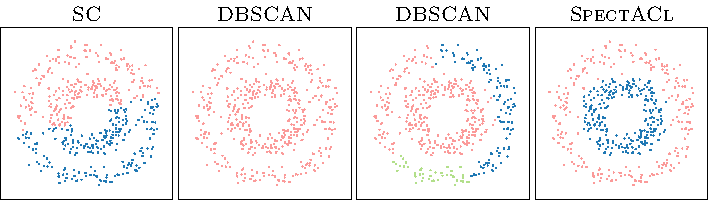
\includegraphics[width=\linewidth]{pics/SAIntroCircles.pdf}
%\documentclass[preview=true]{standalone}
\usepackage{amsmath,amssymb,nicefrac,bbm}
\usepackage{pdfathesis}
\usepackage{etex}
\usepackage{xcolor}
\usepackage[a4paper,left=3.5cm,right=2.5cm,bottom=3.5cm,top=3cm]{geometry}
\usepackage[english]{babel}
\usepackage[round]{natbib}
\usepackage{graphicx,tikz}
\usetikzlibrary{matrix,decorations.pathreplacing, calc, positioning}
\usepackage{relsize} % mathlarger
%\usepackage{hyperref,url}
\usepackage{url}
\usepackage{silence}
\WarningFilter{latex}{Overwriting file}

\usepackage[colorinlistoftodos]{todonotes}
\reversemarginpar
\setlength{\marginparwidth}{3.1cm}
% Theorem-Umgebungen
%\usepackage[amsmath,thmmarks]{ntheorem}
\usepackage{amsthm}
\usepackage{thmtools, thm-restate}
\usepackage{algorithm,algpseudocode}
\algnewcommand{\IIf}[1]{\State\algorithmicif\ #1\ \algorithmicthen}
\algnewcommand{\EndIIf}{\unskip\ \algorithmicend\ \algorithmicif}

\usepackage{enumerate}
\usepackage{booktabs,multirow,adjustbox}
\usepackage[font=small,labelfont=bf]{caption}
\usepackage{subfigure}
\usepackage{pgfplots,filecontents,pgfplotstable}
\usepgfplotslibrary{groupplots}
\pgfplotsset{compat=1.14}
\pgfplotsset{
cohStyle/.style={ctrust,mark options ={ctrust},mark repeat={4}, ultra thick, error bars/.cd,y dir = both, y explicit},
densStyle/.style={cdens,dashed,mark options ={cdens},mark repeat={4}, ultra thick, error bars/.cd,y dir = both, y explicit},
primpStyle/.style={cPrimp,dashed,mark=triangle*,mark options ={cPrimp},mark repeat={3}, ultra thick, error bars/.cd,y dir = both, y explicit},
panStyle/.style={cPan,dashed,mark options ={cPan},mark repeat={3}, ultra thick, error bars/.cd,y dir = both, y explicit},
specStyle/.style={cSpec,mark options ={cSpec},mark repeat={4}, thick, error bars/.cd,y dir = both, y explicit},
specLStyle/.style={cSpecL,mark options ={cSpecL},mark repeat={4}, thick, error bars/.cd,y dir = both, y explicit},
RSCStyle/.style={cRSC,dashed,mark=triangle*,mark options ={cRSC},mark repeat={3}, thick, error bars/.cd,y dir = both, y explicit},
SCStyle/.style={cSC,dashed,mark options ={cSC},mark repeat={3}, thick, error bars/.cd,y dir = both, y explicit},
DBSCANStyle/.style={cDBSCAN,dashed,mark options ={cDBSCAN},mark repeat={3}, thick, error bars/.cd,y dir = both, y explicit},
clusterScatterStyle/.style={scatter/classes={1={cSpecL}, 2={cRSC}, 0={cDBSCAN}, -1={white}},
    scatter, only marks, mark size =0.3, scatter src=explicit symbolic},
nonnegScatterStyle/.style={scatter, only marks, fill=cSpec, scatter src=explicit,
     	visualization depends on ={\thisrow{z} \as \perpointmarksize},
     scatter/@pre marker code/.append style={/tikz/mark size=1.5*\perpointmarksize}},
pandaStyle/.style={cPanda,dashed,mark options ={cPanda},mark repeat={3}, ultra thick, error bars/.cd,y dir = both, y explicit},
punkStyle/.style={cPunk,mark options ={cPunk},mark repeat={3}, thick, error bars/.cd,y dir = both, y explicit},
dbssl1Style/.style={cDBSSL1,dashed,mark options ={cDBSSL1},mark=triangle,mark repeat={3}, thick, error bars/.cd,y dir = both, y explicit},
dbssl2Style/.style={cDBSSL2,dashed,mark options ={cDBSSL2},mark=diamond,mark repeat={3}, thick, error bars/.cd,y dir = both, y explicit},
mdlDbsslStyle/.style={cMDLDBSSL,dashed,mark=star,mark options ={cMDLDBSSL},mark repeat={3}, thick, error bars/.cd,y dir = both, y explicit},
% color change for embedding visualization (fuzzy clusters) 
colormap={test}{[2pt]
    rgb255=(166,206,227);
    rgb255=(166,206,227);
},
}

\Title{ A Mathematical Theory of Making Hard Decisions:
Model Selection and Robustness of Matrix Factorization with Binary
Constraints}

%List of Symbols
\usepackage{nomencl}
\makenomenclature


%\usepackage{color}
\definecolor{col1}{RGB}{166,206,227}
\definecolor{col2}{RGB}{31,120,180}
\definecolor{col3}{RGB}{178,223,138}
\definecolor{col4}{RGB}{51,160,44}
\definecolor{col5}{RGB}{251,154,153}
\definecolor{col6}{RGB}{227,26,28}

\definecolor{cdens}{named}{col1}
\definecolor{ctrust}{named}{col2}
\definecolor{cPrimp}{named}{col3}
\definecolor{cPan}{named}{col4}
\definecolor{cPanda}{named}{col5}
\definecolor{cNassau}{named}{col6}
\definecolor{cMdl4bmf}{named}{col1}


%
\definecolor{cSpec}{named}{col1}
\definecolor{cSpecL}{named}{col2}
\definecolor{cRSC}{named}{col3}
\definecolor{cSC}{named}{col4}
\definecolor{cDBSCAN}{named}{col5}

%
\definecolor{cPunk}{named}{col1}
\definecolor{cDBSSL1}{named}{col2}
\definecolor{cDBSSL2}{named}{col4}
\definecolor{cMDLDBSSL}{named}{col5}
% Theorem-Optionen %
%\theoremseparator{.}
%\newenvironment{proof}{\par\noindent{\textit{ Proof}\ }}{\hfill\qed\\[2mm]}
\theoremstyle{plain}
%\theoremheaderfont{\moon}
%\newcommand{\BlackBox}{\rule{1.5ex}{1.5ex}}  % end of proof
%
\newtheorem{theorem}{Theorem}[chapter]
\newtheorem{corollary}[theorem]{Corollary}
\newtheorem{observation}[theorem]{Observation}
\newtheorem{lemma}[theorem]{Lemma}
%\theorembodyfont{\upshape}
\theoremstyle{definition}
\newtheorem{definition}[theorem]{Definition}
\newtheorem{algSpec}{Algorithm Specification}
\newtheorem*{remark}{Remark}
\newtheorem*{example}{Example}
\newtheorem*{problem}{Problem}

%Operators/Commands
\DeclareMathOperator*{\argmin}{arg\,min}
\DeclareMathOperator*{\argmax}{arg\,max}
\DeclareMathOperator*{\freq}{freq}
\DeclareMathOperator*{\cov}{cov}
\DeclareMathOperator*{\anc}{anc}
\DeclareMathOperator*{\supp}{supp}
\DeclareMathOperator*{\minsup}{minsup}
\DeclareMathOperator*{\tr}{tr}
\DeclareMathOperator*{\bigO}{\mathcal{O}}
\DeclareMathOperator{\diag}{diag}
\DeclareMathOperator{\prox}{prox}
\DeclareMathOperator{\pre}{pre}
\DeclareMathOperator{\rec}{rec}
\newcommand{\Ya}{Y_{\mathcal{J}_a\cdot}}
\newcommand{\Va}{{V_a}}
\newcommand{\Da}{D_{\mathcal{J}_a\cdot}}
\newcommand{\KL}{Kurdyka-{\L}ojasiewicz }
\newcommand{\LXU}{\mathcal{L}}
\newcommand{\F}{\mathcal{F}}
\newcommand{\N}{\mathbb{N}}
\newcommand{\R}{\mathbb{R}}
\newcommand{\estU}{\widetilde{U}_{\widehat{CT}}}
\newcommand{\estu}{\tilde{u}_{\widehat{CT}}}
\newcommand{\estCT}{\widehat{CT}}
\newcommand{\node}{\mathfrak{n}}
\newcommand{\leaf}{\mathfrak{t}}
\newcommand{\krimp}{\textsc{Krimp} }
\newcommand{\shrimp}{\textsc{SHrimp} }
\newcommand{\slim}{\textsc{Slim} }

\makeatletter

\pgfplotstableset{
    zero color/.initial=white,
    zero color/.get=\zerocol,
    zero color/.store in=\zerocol,
    one color/.initial=red,
    one color/.get=\onecol,
    one color/.store in=\onecol,
    color cells/.style={
        every head row/.style={output empty row},
        string type,
        postproc cell content/.code={%
           \pgfkeysalso{@cell content=\rule{0cm}{2.4ex}\cellcolor{\zerocol}
           \pgfmathtruncatemacro\number{int(##1)}
           \ifnum\number>100\cellcolor{\onecol!50!black}
           \else \ifnum\number>0\cellcolor{\onecol!##1}\fi\fi}%
        },
        columns/x/.style={
            column name={},
            postproc cell content/.code={}
        }
    }
}
\makeatother

\makeatletter
\newcommand\footnoteref[1]{\protected@xdef\@thefnmark{\ref{#1}}\@footnotemark}
\makeatother

\makeatletter
%\renewcommand{\@chapapp}{}% Not necessary...
\newenvironment{chapquote}[2][2em]
  {\setlength{\@tempdima}{#1}%
   \def\chapquote@author{#2}%
   \parshape 1 \@tempdima \dimexpr\textwidth-2\@tempdima\relax%
   \itshape}
  {\par\normalfont\hfill--\ \chapquote@author\hspace*{\@tempdima}\par\bigskip}
\makeatother

%Thicker bar
\makeatletter
\newcommand{\thickbar}{\mathpalette\@thickbar}
\newcommand{\@thickbar}[2]{{#1\mkern1.5mu\vbox{
  \sbox\z@{$#1\mkern-1.5mu#2\mkern-1.5mu$}%
  \sbox\tw@{$#1\overline{#2}$}%
  \dimen@=\dimexpr\ht\tw@-\ht\z@-.8\p@\relax
  \hrule\@height.8\p@ % adjust for the desired rule thickness
  \vskip\dimen@
  \box\z@}\mkern1.5mu}
}
\makeatother

%----------box---------------
\usepackage[many]{tcolorbox}
\tcbset{
  myhlight/.style={
    colback=cyan!10,
    arc=0pt,
    outer arc=0pt,
    boxrule=0pt,
    top=2pt,
    bottom=2pt,
    left=2pt,
    right=2pt,
  },
  highlight math style={myhlight},
  mybx/.style={
    colback=white,
    arc=0pt,
    outer arc=0pt,
    boxrule=1pt,
    top=2pt,
    bottom=2pt,
    left=2pt,
    right=2pt,
  }
}

\newtcolorbox{mybox}{
	boxsep=1pt,
  	breakable,
  	mybx
}


% Zeilenabstand einstellen %
\renewcommand{\baselinestretch}{1}
% Floating-Umgebungen anpassen %
\renewcommand{\topfraction}{1.0}
\renewcommand{\bottomfraction}{1.0}
\renewcommand{\floatpagefraction}{1.0}
\renewcommand{\dblfloatpagefraction}{1.0}

% Leere Seite ohne Seitennummer, naechste Seite rechts
\newcommand{\blankpage}{
 \clearpage{\pagestyle{empty}\cleardoublepage}
}

% Keine einzelnen Zeilen beim Anfang eines Abschnitts (Schusterjungen)
\clubpenalty = 10000
% Keine einzelnen Zeilen am Ende eines Abschnitts (Hurenkinder)
\widowpenalty = 10000 \displaywidowpenalty = 10000
% EOF
%
\begin{document}
%
\begin{filecontents}{nmSpectACl_eps.dat}
x y z
1.70069743062 2.42758078324 1
0.285683163483 0.820224134154 1
1.96043338205 1.11652004199 1
2.54379828594 0.801796530514 0
1.02584883691 2.57355440485 1
1.93164886191 1.28604223276 1
1.83409801343 1.05168575212 1
1.50665839702 0.598828682981 0
1.21456049586 1.91816830754 0
0.548489010379 2.4266670795 1
2.43718937566 0.259585631612 0
1.08815940258 1.49111722436 0
1.03453098116 1.5879904518 0
0.109412219779 1.28023561758 1
1.9865620235 1.22135031104 1
1.22512830724 1.0225006133 0
2.86565022133 1.80367677252 0
2.89706812992 1.53195814064 0
0.8209715405 1.72041831352 0
0.617806017378 2.40727584262 1
2.28442347034 0.430331423047 0
1.28180236997 1.03358907376 0
0.887937054635 2.68053646933 1
0.891570602061 2.32922789032 1
2.65618201755 0.894877000626 0
0.498394232883 2.45236217747 1
1.35694280656 2.46718908062 1
1.11489573331 1.85699692515 0
2.9080680088 1.73914577833 0
0.785679177354 2.44215259264 1
0.196823873853 1.89256063131 1
1.17823524744 1.75551785493 0
1.23992030311 2.66315904413 1
2.00540849232 0.499253921452 0
0.848956944163 2.45868527982 1
0.0925078051445 1.29305455349 1
0.247138803261 1.95645113223 1
2.83766305835 1.76420767232 0
1.12807120931 1.38527205119 0
1.94201627226 1.40478582163 1
1.25729757329 1.8930319065 0
1.89326303725 1.91932512895 1
1.72383858092 2.21738324713 1
0.45709546568 2.4199525741 1
1.35307081946 2.21860026432 1
1.00887362506 1.94033464961 0
2.34181723671 0.686515872943 0
1.11475444609 0.954182702693 0
0.420448354856 2.32241979328 1
1.59149868632 2.16078316015 1
0.329310350731 1.82923651818 1
0.629423152641 2.36690609361 1
0.307287028638 1.63670049795 1
2.59724264213 0.569519846613 0
0.527392241622 2.54113453641 1
1.91786921713 0.481595165812 0
1.95156790129 2.12611147089 1
1.41194255779 2.66793976628 1
0.0694222959687 1.82183402009 1
1.61367440743 0.544603242775 0
1.84906416078 1.43524726088 1
2.56840153548 0.978613872479 0
2.68782194498 1.60369331079 0
1.6967066369 2.05018333769 1
0.287779916276 1.35181404437 1
2.10581182305 0.58600544124 0
2.76589189346 1.31793021207 0
0.903330891708 2.71981111471 1
1.78910702143 1.78431684787 1
2.85201486168 1.75683049978 0
2.61444426339 1.1421123448 0
1.76686652891 0.412643118932 0
2.38343223857 0.614019382719 0
0.351982420161 1.82124180438 1
1.20104638372 1.08550087193 0
1.71310358783 2.10563588448 1
1.20574320869 1.14241676927 0
1.85476278831 1.68570217527 1
0.866928473775 2.71912423537 1
1.24150157057 1.87008926301 0
1.28290021851 2.54224942198 1
2.20513157208 0.332694252519 0
0.7649274204 2.49776682771 1
1.92833706433 1.74896192577 1
1.12650480957 1.0348913114 0
0.42035554481 2.29433128095 1
1.8227778128 1.73009804176 1
1.40440087482 0.800372448393 0
0.350170029196 1.83113326458 1
2.67833915261 0.955760684365 0
1.45206309833 2.3376423972 1
1.99881809264 0.647288007188 0
1.73930300342 2.27513141315 1
0.997530664835 2.48601880132 1
2.52748209417 0.964779854994 0
0.18616961175 1.41798846544 1
1.27951506157 0.579681303838 0
1.24451979199 1.01467765734 0
1.528155426 0.429507299506 0
1.86116862662 0.0 0
0.229448043123 1.39451828581 1
2.43840791486 0.811277652094 0
1.08024324217 1.45606914327 0
1.69141952321 1.87996999864 1
0.523342152062 2.27879186696 1
2.53685907702 0.842989476903 0
0.781622595306 2.37059793943 1
2.37151355968 0.752368295204 0
1.81585388656 0.405096626174 0
0.526353426641 2.28139242049 1
2.7760661566 0.95760548246 0
0.923603269543 2.64416122336 1
1.94640723913 1.91848140563 1
1.56063634725 2.50248629435 1
1.0176090148 2.72395908515 1
2.31363407826 0.5281707426 0
1.73803401456 1.88934225142 1
0.26732734312 1.01993624365 1
1.92620482073 1.36669614426 1
2.83528847849 2.08551281403 0
1.2560191234 0.92058406981 0
2.38592708362 0.628151589247 0
1.63132977838 0.709002849989 0
1.05904065429 1.51493849809 0
0.139685121871 1.80990844772 1
1.27499215905 1.06475398303 0
1.14937169414 1.42166121091 0
2.33215946967 0.30036289709 0
1.67510627109 0.411176705111 0
1.18231701939 2.50556350357 1
1.77038669418 1.7965018847 1
2.41711258717 1.06425648687 0
1.5466743199 2.19799847606 1
2.81159915284 0.84108084496 0
2.09568775447 0.361760404015 0
1.62856213766 2.40924498166 1
2.39833092966 0.493171096231 0
1.51465143737 2.47271499647 1
1.13635348992 0.947616890809 0
1.04349043595 1.39023226786 0
0.603031169212 2.58849736575 1
1.9387998979 1.22409851527 1
0.128778294394 1.31392528176 1
1.1003283767 1.2661573588 0
0.743838019158 2.52252993124 1
0.61621116068 2.65631385961 1
0.886728816447 2.57220887 1
1.93703048927 0.497335966775 0
1.34132891502 0.890984584948 0
0.536517048738 2.03140735086 1
0.426818260547 2.19895923382 1
0.382225086449 2.24212488028 1
0.90075749994 2.84889611659 1
1.71053267234 0.139893439754 0
1.29639938455 2.59086974776 1
1.94208010739 0.301786108633 0
1.83766716651 1.89862578133 1
0.217910019358 1.18284981176 1
2.87431916031 1.13362681065 0
2.49128297904 0.808660342234 0
0.887367512053 1.77483826418 0
2.41849255062 0.5324350021 0
1.52025137653 2.40917722219 1
2.81144168216 1.32711652029 0
1.04959124228 1.45154913004 0
2.76797402357 1.57360077806 0
1.82169413997 1.6359444949 1
0.463673012107 2.13666946634 1
1.76717691103 0.185518641762 0
1.79700009392 0.415992627791 0
1.07371926343 1.25433471066 0
0.35340797154 2.20777111939 1
0.910470573245 2.57545855259 1
1.00666113925 1.41487472942 0
0.263242311008 2.11420843779 1
1.83750587555 0.960921001284 1
0.598118607947 2.17126465619 1
0.989607517794 2.72016213659 1
0.339991852275 1.6367039174 1
2.81553150588 1.25227670267 0
1.1688157054 1.61925018628 0
2.87702213607 1.62065697172 0
1.18784418709 1.07176694342 0
2.69535677668 1.14397649917 0
2.61215137255 0.908888019432 0
2.2703000471 0.739737480907 0
0.310292767944 1.5927524401 1
1.9751498572 1.39478059397 1
1.05585797661 1.86898397783 0
0.491864333665 2.31875950071 1
2.04280176433 0.227220807369 0
1.29239733899 2.77729312657 1
1.76399564245 0.389462528366 0
1.10987143975 2.45825835483 1
0.888789567782 2.65387087803 1
2.45980643174 0.992909318285 0
1.08897922761 1.42887358233 0
0.759086710455 2.40740216785 1
2.85579700003 1.62503776295 0
1.49047821489 0.578651837622 0
2.14306688802 0.410252695811 0
2.80690341525 1.04739831031 0
1.08084426927 2.37142988192 1
1.24156411616 1.55517287562 0
1.46082893365 0.841033454439 0
1.13147127699 2.53816467841 1
2.47534170514 0.691577879525 0
0.515186721621 2.37712522384 1
0.738658590011 2.23721041569 1
0.152209727518 1.84671174913 1
2.60849673113 0.841526842613 0
1.04231829692 2.71045161422 1
0.964376417508 1.74174356827 0
0.342359603748 2.31301969708 1
0.312328480287 2.0697583552 1
2.45657728683 0.742808305141 0
1.96519472004 1.95521093343 1
0.976026718348 1.65145435908 0
1.70038574297 0.690680548668 0
1.37321471501 0.593617808351 0
1.34431592493 2.38004670142 1
1.20432098055 1.41547092441 0
1.0929063259 1.64510555084 0
1.14149626236 1.27251025565 0
2.38350457204 0.579440777335 0
1.29738017256 2.28865081481 1
1.19200628952 1.85807567095 0
2.29057019712 0.494581835568 0
1.80036719203 2.25739553896 1
1.7374178378 0.17861431239 0
0.681070242517 2.21529849059 1
1.88653779019 1.71753481275 1
1.66130686 0.453575429025 0
1.05708950661 1.30651646662 0
1.7262189757 2.0892030765 1
1.8743608435 1.34263072606 1
1.48620524338 0.715922906298 0
2.00459538411 0.635140423792 0
0.318587109448 1.92679150556 1
1.37843639956 0.707088283144 0
2.60563623353 0.84239504921 0
2.51013047406 1.15186988552 0
1.09765232658 2.56485848597 1
2.65051441579 0.706858112677 0
0.352710453599 1.60528124984 1
1.367034677 2.342617793 1
2.6778340428 1.27583043688 0
2.77041498717 1.62149290572 0
0.433413700012 2.28661466553 1
2.48279234082 0.838028620621 0
0.664103039947 2.61890924636 1
0.485901366946 2.02729851019 1
1.85342076722 0.311040878791 0
2.24141958751 0.69211889508 0
1.05284501061 0.815302813624 0
1.79533297587 1.72925735288 1
1.59592524946 2.291103752 1
1.12311889981 2.73494294316 1
0.239642607379 1.4708710286 1
2.38074908517 0.178741070048 0
1.95942048639 0.485758418579 0
0.801008762883 2.35832224956 1
1.74336065112 2.52814028379 1
2.00425063315 1.44973882129 1
2.99874263731 1.61490975065 0
1.77010542011 2.37104764753 1
1.512850527 2.28856440723 1
2.45235640311 0.561489373791 0
1.295122251 0.789267498929 0
1.51455075898 0.528202376017 0
0.304527789681 1.21175257382 1
1.21559659311 0.781644945741 0
2.13154242053 0.328030655553 0
1.02901463251 1.60574602789 0
1.04967754137 2.46974317694 1
0.383986869727 1.946959298 1
0.674587230211 2.31409008533 1
2.94816733924 1.82970946363 0
1.46163323762 0.792251773345 0
0.660363196201 2.44792160823 1
2.03001716038 0.213480207542 0
1.36368239515 0.799287249057 0
0.100287359104 1.22065856204 1
2.01060150251 0.464874464476 0
2.02983745816 0.305243543361 0
1.2251556746 1.52746937796 0
2.69691681725 1.71441309537 0
2.85609415251 1.41314756677 0
1.01887468848 2.53297875059 1
1.72087173411 1.97290485697 1
0.0540782987346 1.66034457313 1
1.50772484392 0.172194489983 0
1.24910710679 0.732983283934 0
1.21965279462 1.48366422323 0
1.62105492439 2.04589281976 1
2.87108229353 1.48089493044 0
2.86550061675 1.67997945483 0
1.09627892364 1.65438075877 0
0.338132847221 1.79813179713 1
0.436675834273 2.29829461324 1
1.35612302258 0.617635762047 0
2.71578839431 1.11238360205 0
1.84067753076 2.35076159932 1
1.90883244213 1.40654781879 1
0.448930144962 2.42194163441 1
2.27088828505 0.720328288284 0
1.99427584167 0.292469923157 0
2.05179138307 0.075191975576 0
2.75775762337 1.41657699478 0
0.12405803592 1.67542521447 1
2.43818544068 0.725956693576 0
0.312635410658 1.46319738786 1
0.191240314346 1.65611706549 1
2.75529018146 1.51664712917 0
2.87438941247 1.42513159143 0
1.6124710734 0.108162333984 0
2.07748229347 1.37016700533 1
1.34233953375 0.80510418713 0
0.402666931541 1.97206849653 1
1.59991006122 0.430928345538 0
1.76450324322 1.9417972377 1
0.68142574163 2.3657937995 1
0.164887719809 0.933208295559 1
0.917202040984 2.45367836822 1
0.162413262346 1.79806447542 1
1.69954497521 0.474876958658 0
0.885974873525 2.80037127387 1
1.51432134071 2.26982073221 1
1.34621921819 0.906396320943 0
0.691126264848 2.70915758443 1
1.87293313667 1.78727508456 1
2.28649531765 0.726889577091 0
1.07263048888 2.68627388773 1
1.80060022058 0.599304932113 0
1.26924503947 2.54861366445 1
1.05684697644 1.91308852172 0
1.34125453355 0.95711539541 0
2.8125803328 1.52002754851 0
1.21682707227 0.904424035905 0
1.31929933512 2.79201230232 1
0.637404952623 2.32382669843 1
2.17137726399 0.282323068269 0
1.62762538368 2.26290014007 1
0.540666367159 2.33600275939 1
1.88293690233 1.28480350699 1
2.77912006373 1.9726418669 0
0.887955978785 2.55238946452 1
1.85499981106 2.17561046177 1
2.77275743931 1.26672052764 0
1.88408081212 1.55654855145 1
2.20422656878 0.194151609861 0
1.37215670775 0.64239160578 0
2.74173332893 1.06281332167 0
1.3519692899 2.44789629152 1
0.976624716971 1.76062464088 0
1.04508085459 1.58720561346 0
1.86316148119 0.606405006819 0
1.84838679137 0.364768005124 0
0.3387851597 2.31151471375 1
0.695323634969 2.53219749966 1
1.5016800772 2.28286263615 1
1.72601415658 0.425192245283 0
2.7956168279 1.41300555516 0
0.575132420922 2.21555668975 1
1.92736865662 1.30428244235 1
2.86941042658 1.12652831483 0
0.505972295319 2.11848657916 1
2.88083111935 1.79685857086 0
1.54968608895 2.50447888087 1
2.31278971533 0.259675335988 0
2.73879578515 1.18969715242 0
2.41045930274 0.901294611205 0
0.174601175717 1.25065471515 1
2.32186139204 0.515582850319 0
0.20554231582 1.35225498011 1
2.73059185626 1.20383151563 0
1.3865034904 2.53822490098 1
1.12900900657 2.75114078017 1
0.115069738958 1.04596772082 1
1.335120272 2.64619551797 1
0.831696677651 2.37593629365 1
0.292063587839 1.88454278761 1
1.40477301971 2.48630866567 1
0.227853652523 1.72614884781 1
1.39895080992 2.73195382504 1
2.74706816704 1.76622164219 0
1.65483832512 2.04749839106 1
1.9617597714 0.486798653141 0
1.64888491758 2.17115329123 1
1.60586723589 0.501084875631 0
0.284675287626 1.34679532238 1
1.7675237627 2.24242168385 1
1.26193391783 2.60789114088 1
1.85894079362 1.62496524757 1
1.23674367127 0.982304806675 0
1.97582138089 0.509380358308 0
1.05600781745 2.677392365 1
0.184110621272 2.05447883901 1
0.547385160286 2.55233290655 1
2.57887948172 0.828032733195 0
0.207424483914 1.40821380306 1
1.4369592134 2.72855234245 1
1.62259449811 1.74010086385 1
2.672451501 1.6291678069 0
1.81325243451 0.253878981216 0
1.6389068495 2.55396535903 1
1.78009058629 1.82382255609 1
1.82405310361 2.18872776439 1
0.297924979561 2.15608602252 1
0.734938555418 2.43601614007 1
2.76539867309 0.876829399765 0
0.299689834261 2.26240499707 1
0.657100676443 2.54932984854 1
1.97531757625 0.418517119017 0
1.70335971574 2.01957604536 1
2.01136443846 1.56650446432 1
1.9889246753 1.33708935655 1
0.520697457737 2.19392438309 1
0.201610918869 1.11114702728 1
1.18460310214 2.64018309532 1
1.67953679203 2.09096852593 1
2.52903300028 0.668689176375 0
1.82992609123 0.41148308689 0
1.8782077118 1.15964218423 1
2.77296228387 1.32572928549 0
1.82869717065 0.425653875063 0
0.894053475273 2.44439263156 1
1.07621362954 1.70969278243 0
1.45644007418 2.18215955599 1
1.22063523709 1.744321168 0
1.07967091239 1.06274577676 0
1.1900696085 1.26923933736 0
1.04550909582 1.95159439522 0
1.36599613108 0.996983555907 0
1.48939507438 2.55035208922 1
1.39352940488 0.963024804974 0
1.79847337348 1.76745116277 1
2.79775175948 0.989798501929 0
1.85447215813 0.591984136577 0
1.97133310695 1.23755879013 1
1.33548899995 0.903694832059 0
1.24331015073 2.6153250888 1
1.18889713657 2.78378504495 1
0.959819003516 1.85803345242 0
1.48688739481 0.518828000145 0
2.17038326017 0.538678939108 0
2.00401389267 1.2148267132 1
1.80471537631 1.56843402421 1
2.41227229935 0.418729119508 0
1.54810143205 0.592880123322 0
2.70786075559 1.37847478472 0
1.95754047284 1.18045687789 1
0.376516805236 1.88573157828 1
1.55659448472 1.89138211448 1
1.6713666353 0.452084078249 0
2.01552714856 0.493164592727 0
2.92882892778 1.71535055117 0
2.30685921255 0.69876892802 0
0.910811583335 2.47994266873 1
1.20418470115 2.33843955069 1
2.39790481126 0.794684627456 0
2.46701618738 0.581809838238 0
0.251366988518 1.8780274577 1
0.499412691579 2.38088700981 1
2.56205261531 0.65140655269 0
0.421518010626 2.06060390571 1
1.17009887948 1.5134267149 0
2.81288537691 1.68955621988 0
1.85801783879 0.555828770401 0
1.62002253434 2.06714531107 1
0.587232551254 2.47998567591 1
0.929550119504 2.62696249914 1
0.285941297863 1.76825739547 1
0.259015697972 1.26276981669 1
1.90778512029 1.51870006004 1
1.78857330267 0.328932520462 0
1.62111786442 2.21583017128 1
1.55851506264 2.39564830468 1
2.8184718636 1.49831763883 0
1.44366997728 0.811031572419 0
0.670803912622 2.52569944579 1
1.99900347199 1.27336970112 1
1.03545744455 2.67615661925 1
1.94020677429 0.417071861833 0
1.7209951759 0.415479497045 0
2.44397592822 0.627725787503 0
1.38008876818 0.718105733857 0
2.53036245288 0.380380389259 0
1.95319494442 0.992058285038 1
0.983756955407 1.32684250689 0
0.6881145508 2.71837116248 1
1.88019132883 1.60123260018 1
1.29417582527 1.2231395338 0
1.29745287353 2.79297372882 1
0.333622187036 2.26301752448 1
0.32392659893 1.70725807039 1
1.27163496314 2.5038370693 1
0.419549967659 2.16152124321 1
0.70356632396 2.43698318681 1
2.24311863984 0.0606826745953 0
\end{filecontents}
\begin{filecontents}{nmSpectACl_knn_n.dat}
x y z
1.70069743062 2.42758078324 1
0.285683163483 0.820224134154 1
1.96043338205 1.11652004199 1
2.54379828594 0.801796530514 0
1.02584883691 2.57355440485 1
1.93164886191 1.28604223276 1
1.83409801343 1.05168575212 1
1.50665839702 0.598828682981 0
1.21456049586 1.91816830754 0
0.548489010379 2.4266670795 1
2.43718937566 0.259585631612 0
1.08815940258 1.49111722436 0
1.03453098116 1.5879904518 0
0.109412219779 1.28023561758 1
1.9865620235 1.22135031104 1
1.22512830724 1.0225006133 0
2.86565022133 1.80367677252 0
2.89706812992 1.53195814064 0
0.8209715405 1.72041831352 0
0.617806017378 2.40727584262 1
2.28442347034 0.430331423047 0
1.28180236997 1.03358907376 0
0.887937054635 2.68053646933 1
0.891570602061 2.32922789032 1
2.65618201755 0.894877000626 0
0.498394232883 2.45236217747 1
1.35694280656 2.46718908062 1
1.11489573331 1.85699692515 0
2.9080680088 1.73914577833 0
0.785679177354 2.44215259264 1
0.196823873853 1.89256063131 1
1.17823524744 1.75551785493 0
1.23992030311 2.66315904413 1
2.00540849232 0.499253921452 0
0.848956944163 2.45868527982 1
0.0925078051445 1.29305455349 1
0.247138803261 1.95645113223 1
2.83766305835 1.76420767232 0
1.12807120931 1.38527205119 0
1.94201627226 1.40478582163 1
1.25729757329 1.8930319065 0
1.89326303725 1.91932512895 1
1.72383858092 2.21738324713 1
0.45709546568 2.4199525741 1
1.35307081946 2.21860026432 1
1.00887362506 1.94033464961 0
2.34181723671 0.686515872943 0
1.11475444609 0.954182702693 0
0.420448354856 2.32241979328 1
1.59149868632 2.16078316015 1
0.329310350731 1.82923651818 1
0.629423152641 2.36690609361 1
0.307287028638 1.63670049795 1
2.59724264213 0.569519846613 0
0.527392241622 2.54113453641 1
1.91786921713 0.481595165812 0
1.95156790129 2.12611147089 1
1.41194255779 2.66793976628 1
0.0694222959687 1.82183402009 1
1.61367440743 0.544603242775 0
1.84906416078 1.43524726088 1
2.56840153548 0.978613872479 0
2.68782194498 1.60369331079 0
1.6967066369 2.05018333769 1
0.287779916276 1.35181404437 1
2.10581182305 0.58600544124 0
2.76589189346 1.31793021207 0
0.903330891708 2.71981111471 1
1.78910702143 1.78431684787 1
2.85201486168 1.75683049978 0
2.61444426339 1.1421123448 0
1.76686652891 0.412643118932 0
2.38343223857 0.614019382719 0
0.351982420161 1.82124180438 1
1.20104638372 1.08550087193 0
1.71310358783 2.10563588448 1
1.20574320869 1.14241676927 0
1.85476278831 1.68570217527 1
0.866928473775 2.71912423537 1
1.24150157057 1.87008926301 0
1.28290021851 2.54224942198 1
2.20513157208 0.332694252519 0
0.7649274204 2.49776682771 1
1.92833706433 1.74896192577 1
1.12650480957 1.0348913114 0
0.42035554481 2.29433128095 1
1.8227778128 1.73009804176 1
1.40440087482 0.800372448393 0
0.350170029196 1.83113326458 1
2.67833915261 0.955760684365 0
1.45206309833 2.3376423972 1
1.99881809264 0.647288007188 0
1.73930300342 2.27513141315 1
0.997530664835 2.48601880132 1
2.52748209417 0.964779854994 0
0.18616961175 1.41798846544 1
1.27951506157 0.579681303838 0
1.24451979199 1.01467765734 0
1.528155426 0.429507299506 0
1.86116862662 0.0 0
0.229448043123 1.39451828581 1
2.43840791486 0.811277652094 0
1.08024324217 1.45606914327 0
1.69141952321 1.87996999864 1
0.523342152062 2.27879186696 1
2.53685907702 0.842989476903 0
0.781622595306 2.37059793943 1
2.37151355968 0.752368295204 0
1.81585388656 0.405096626174 0
0.526353426641 2.28139242049 1
2.7760661566 0.95760548246 0
0.923603269543 2.64416122336 1
1.94640723913 1.91848140563 1
1.56063634725 2.50248629435 1
1.0176090148 2.72395908515 1
2.31363407826 0.5281707426 0
1.73803401456 1.88934225142 1
0.26732734312 1.01993624365 1
1.92620482073 1.36669614426 1
2.83528847849 2.08551281403 0
1.2560191234 0.92058406981 0
2.38592708362 0.628151589247 0
1.63132977838 0.709002849989 0
1.05904065429 1.51493849809 0
0.139685121871 1.80990844772 1
1.27499215905 1.06475398303 0
1.14937169414 1.42166121091 0
2.33215946967 0.30036289709 0
1.67510627109 0.411176705111 0
1.18231701939 2.50556350357 1
1.77038669418 1.7965018847 1
2.41711258717 1.06425648687 0
1.5466743199 2.19799847606 1
2.81159915284 0.84108084496 0
2.09568775447 0.361760404015 0
1.62856213766 2.40924498166 1
2.39833092966 0.493171096231 0
1.51465143737 2.47271499647 1
1.13635348992 0.947616890809 0
1.04349043595 1.39023226786 0
0.603031169212 2.58849736575 1
1.9387998979 1.22409851527 1
0.128778294394 1.31392528176 1
1.1003283767 1.2661573588 0
0.743838019158 2.52252993124 1
0.61621116068 2.65631385961 1
0.886728816447 2.57220887 1
1.93703048927 0.497335966775 0
1.34132891502 0.890984584948 0
0.536517048738 2.03140735086 1
0.426818260547 2.19895923382 1
0.382225086449 2.24212488028 1
0.90075749994 2.84889611659 1
1.71053267234 0.139893439754 0
1.29639938455 2.59086974776 1
1.94208010739 0.301786108633 0
1.83766716651 1.89862578133 1
0.217910019358 1.18284981176 1
2.87431916031 1.13362681065 0
2.49128297904 0.808660342234 0
0.887367512053 1.77483826418 0
2.41849255062 0.5324350021 0
1.52025137653 2.40917722219 1
2.81144168216 1.32711652029 0
1.04959124228 1.45154913004 0
2.76797402357 1.57360077806 0
1.82169413997 1.6359444949 1
0.463673012107 2.13666946634 1
1.76717691103 0.185518641762 0
1.79700009392 0.415992627791 0
1.07371926343 1.25433471066 0
0.35340797154 2.20777111939 1
0.910470573245 2.57545855259 1
1.00666113925 1.41487472942 0
0.263242311008 2.11420843779 1
1.83750587555 0.960921001284 1
0.598118607947 2.17126465619 1
0.989607517794 2.72016213659 1
0.339991852275 1.6367039174 1
2.81553150588 1.25227670267 0
1.1688157054 1.61925018628 0
2.87702213607 1.62065697172 0
1.18784418709 1.07176694342 0
2.69535677668 1.14397649917 0
2.61215137255 0.908888019432 0
2.2703000471 0.739737480907 0
0.310292767944 1.5927524401 1
1.9751498572 1.39478059397 1
1.05585797661 1.86898397783 0
0.491864333665 2.31875950071 1
2.04280176433 0.227220807369 0
1.29239733899 2.77729312657 1
1.76399564245 0.389462528366 0
1.10987143975 2.45825835483 1
0.888789567782 2.65387087803 1
2.45980643174 0.992909318285 0
1.08897922761 1.42887358233 0
0.759086710455 2.40740216785 1
2.85579700003 1.62503776295 0
1.49047821489 0.578651837622 0
2.14306688802 0.410252695811 0
2.80690341525 1.04739831031 0
1.08084426927 2.37142988192 1
1.24156411616 1.55517287562 0
1.46082893365 0.841033454439 0
1.13147127699 2.53816467841 1
2.47534170514 0.691577879525 0
0.515186721621 2.37712522384 1
0.738658590011 2.23721041569 1
0.152209727518 1.84671174913 1
2.60849673113 0.841526842613 0
1.04231829692 2.71045161422 1
0.964376417508 1.74174356827 0
0.342359603748 2.31301969708 1
0.312328480287 2.0697583552 1
2.45657728683 0.742808305141 0
1.96519472004 1.95521093343 1
0.976026718348 1.65145435908 0
1.70038574297 0.690680548668 0
1.37321471501 0.593617808351 0
1.34431592493 2.38004670142 1
1.20432098055 1.41547092441 0
1.0929063259 1.64510555084 0
1.14149626236 1.27251025565 0
2.38350457204 0.579440777335 0
1.29738017256 2.28865081481 1
1.19200628952 1.85807567095 0
2.29057019712 0.494581835568 0
1.80036719203 2.25739553896 1
1.7374178378 0.17861431239 0
0.681070242517 2.21529849059 1
1.88653779019 1.71753481275 1
1.66130686 0.453575429025 0
1.05708950661 1.30651646662 0
1.7262189757 2.0892030765 1
1.8743608435 1.34263072606 1
1.48620524338 0.715922906298 0
2.00459538411 0.635140423792 0
0.318587109448 1.92679150556 1
1.37843639956 0.707088283144 0
2.60563623353 0.84239504921 0
2.51013047406 1.15186988552 0
1.09765232658 2.56485848597 1
2.65051441579 0.706858112677 0
0.352710453599 1.60528124984 1
1.367034677 2.342617793 1
2.6778340428 1.27583043688 0
2.77041498717 1.62149290572 0
0.433413700012 2.28661466553 1
2.48279234082 0.838028620621 0
0.664103039947 2.61890924636 1
0.485901366946 2.02729851019 1
1.85342076722 0.311040878791 0
2.24141958751 0.69211889508 0
1.05284501061 0.815302813624 0
1.79533297587 1.72925735288 1
1.59592524946 2.291103752 1
1.12311889981 2.73494294316 1
0.239642607379 1.4708710286 1
2.38074908517 0.178741070048 0
1.95942048639 0.485758418579 0
0.801008762883 2.35832224956 1
1.74336065112 2.52814028379 1
2.00425063315 1.44973882129 1
2.99874263731 1.61490975065 0
1.77010542011 2.37104764753 1
1.512850527 2.28856440723 1
2.45235640311 0.561489373791 0
1.295122251 0.789267498929 0
1.51455075898 0.528202376017 0
0.304527789681 1.21175257382 1
1.21559659311 0.781644945741 0
2.13154242053 0.328030655553 0
1.02901463251 1.60574602789 0
1.04967754137 2.46974317694 1
0.383986869727 1.946959298 1
0.674587230211 2.31409008533 1
2.94816733924 1.82970946363 0
1.46163323762 0.792251773345 0
0.660363196201 2.44792160823 1
2.03001716038 0.213480207542 0
1.36368239515 0.799287249057 0
0.100287359104 1.22065856204 1
2.01060150251 0.464874464476 0
2.02983745816 0.305243543361 0
1.2251556746 1.52746937796 0
2.69691681725 1.71441309537 0
2.85609415251 1.41314756677 0
1.01887468848 2.53297875059 1
1.72087173411 1.97290485697 1
0.0540782987346 1.66034457313 1
1.50772484392 0.172194489983 0
1.24910710679 0.732983283934 0
1.21965279462 1.48366422323 0
1.62105492439 2.04589281976 1
2.87108229353 1.48089493044 0
2.86550061675 1.67997945483 0
1.09627892364 1.65438075877 0
0.338132847221 1.79813179713 1
0.436675834273 2.29829461324 1
1.35612302258 0.617635762047 0
2.71578839431 1.11238360205 0
1.84067753076 2.35076159932 1
1.90883244213 1.40654781879 1
0.448930144962 2.42194163441 1
2.27088828505 0.720328288284 0
1.99427584167 0.292469923157 0
2.05179138307 0.075191975576 0
2.75775762337 1.41657699478 0
0.12405803592 1.67542521447 1
2.43818544068 0.725956693576 0
0.312635410658 1.46319738786 1
0.191240314346 1.65611706549 1
2.75529018146 1.51664712917 0
2.87438941247 1.42513159143 0
1.6124710734 0.108162333984 0
2.07748229347 1.37016700533 1
1.34233953375 0.80510418713 0
0.402666931541 1.97206849653 1
1.59991006122 0.430928345538 0
1.76450324322 1.9417972377 1
0.68142574163 2.3657937995 1
0.164887719809 0.933208295559 1
0.917202040984 2.45367836822 1
0.162413262346 1.79806447542 1
1.69954497521 0.474876958658 0
0.885974873525 2.80037127387 1
1.51432134071 2.26982073221 1
1.34621921819 0.906396320943 0
0.691126264848 2.70915758443 1
1.87293313667 1.78727508456 1
2.28649531765 0.726889577091 0
1.07263048888 2.68627388773 1
1.80060022058 0.599304932113 0
1.26924503947 2.54861366445 1
1.05684697644 1.91308852172 0
1.34125453355 0.95711539541 0
2.8125803328 1.52002754851 0
1.21682707227 0.904424035905 0
1.31929933512 2.79201230232 1
0.637404952623 2.32382669843 1
2.17137726399 0.282323068269 0
1.62762538368 2.26290014007 1
0.540666367159 2.33600275939 1
1.88293690233 1.28480350699 1
2.77912006373 1.9726418669 0
0.887955978785 2.55238946452 1
1.85499981106 2.17561046177 1
2.77275743931 1.26672052764 0
1.88408081212 1.55654855145 1
2.20422656878 0.194151609861 0
1.37215670775 0.64239160578 0
2.74173332893 1.06281332167 0
1.3519692899 2.44789629152 1
0.976624716971 1.76062464088 0
1.04508085459 1.58720561346 0
1.86316148119 0.606405006819 0
1.84838679137 0.364768005124 0
0.3387851597 2.31151471375 1
0.695323634969 2.53219749966 1
1.5016800772 2.28286263615 1
1.72601415658 0.425192245283 0
2.7956168279 1.41300555516 0
0.575132420922 2.21555668975 1
1.92736865662 1.30428244235 1
2.86941042658 1.12652831483 0
0.505972295319 2.11848657916 1
2.88083111935 1.79685857086 0
1.54968608895 2.50447888087 1
2.31278971533 0.259675335988 0
2.73879578515 1.18969715242 0
2.41045930274 0.901294611205 0
0.174601175717 1.25065471515 1
2.32186139204 0.515582850319 0
0.20554231582 1.35225498011 1
2.73059185626 1.20383151563 0
1.3865034904 2.53822490098 1
1.12900900657 2.75114078017 1
0.115069738958 1.04596772082 1
1.335120272 2.64619551797 1
0.831696677651 2.37593629365 1
0.292063587839 1.88454278761 1
1.40477301971 2.48630866567 1
0.227853652523 1.72614884781 1
1.39895080992 2.73195382504 1
2.74706816704 1.76622164219 0
1.65483832512 2.04749839106 1
1.9617597714 0.486798653141 0
1.64888491758 2.17115329123 1
1.60586723589 0.501084875631 0
0.284675287626 1.34679532238 1
1.7675237627 2.24242168385 1
1.26193391783 2.60789114088 1
1.85894079362 1.62496524757 1
1.23674367127 0.982304806675 0
1.97582138089 0.509380358308 0
1.05600781745 2.677392365 1
0.184110621272 2.05447883901 1
0.547385160286 2.55233290655 1
2.57887948172 0.828032733195 0
0.207424483914 1.40821380306 1
1.4369592134 2.72855234245 1
1.62259449811 1.74010086385 1
2.672451501 1.6291678069 0
1.81325243451 0.253878981216 0
1.6389068495 2.55396535903 1
1.78009058629 1.82382255609 1
1.82405310361 2.18872776439 1
0.297924979561 2.15608602252 1
0.734938555418 2.43601614007 1
2.76539867309 0.876829399765 0
0.299689834261 2.26240499707 1
0.657100676443 2.54932984854 1
1.97531757625 0.418517119017 0
1.70335971574 2.01957604536 1
2.01136443846 1.56650446432 1
1.9889246753 1.33708935655 1
0.520697457737 2.19392438309 1
0.201610918869 1.11114702728 1
1.18460310214 2.64018309532 1
1.67953679203 2.09096852593 1
2.52903300028 0.668689176375 0
1.82992609123 0.41148308689 0
1.8782077118 1.15964218423 1
2.77296228387 1.32572928549 0
1.82869717065 0.425653875063 0
0.894053475273 2.44439263156 1
1.07621362954 1.70969278243 0
1.45644007418 2.18215955599 1
1.22063523709 1.744321168 0
1.07967091239 1.06274577676 0
1.1900696085 1.26923933736 0
1.04550909582 1.95159439522 0
1.36599613108 0.996983555907 0
1.48939507438 2.55035208922 1
1.39352940488 0.963024804974 0
1.79847337348 1.76745116277 1
2.79775175948 0.989798501929 0
1.85447215813 0.591984136577 0
1.97133310695 1.23755879013 1
1.33548899995 0.903694832059 0
1.24331015073 2.6153250888 1
1.18889713657 2.78378504495 1
0.959819003516 1.85803345242 0
1.48688739481 0.518828000145 0
2.17038326017 0.538678939108 0
2.00401389267 1.2148267132 1
1.80471537631 1.56843402421 1
2.41227229935 0.418729119508 0
1.54810143205 0.592880123322 0
2.70786075559 1.37847478472 0
1.95754047284 1.18045687789 1
0.376516805236 1.88573157828 1
1.55659448472 1.89138211448 1
1.6713666353 0.452084078249 0
2.01552714856 0.493164592727 0
2.92882892778 1.71535055117 0
2.30685921255 0.69876892802 0
0.910811583335 2.47994266873 1
1.20418470115 2.33843955069 1
2.39790481126 0.794684627456 0
2.46701618738 0.581809838238 0
0.251366988518 1.8780274577 1
0.499412691579 2.38088700981 1
2.56205261531 0.65140655269 0
0.421518010626 2.06060390571 1
1.17009887948 1.5134267149 0
2.81288537691 1.68955621988 0
1.85801783879 0.555828770401 0
1.62002253434 2.06714531107 1
0.587232551254 2.47998567591 1
0.929550119504 2.62696249914 1
0.285941297863 1.76825739547 1
0.259015697972 1.26276981669 1
1.90778512029 1.51870006004 1
1.78857330267 0.328932520462 0
1.62111786442 2.21583017128 1
1.55851506264 2.39564830468 1
2.8184718636 1.49831763883 0
1.44366997728 0.811031572419 0
0.670803912622 2.52569944579 1
1.99900347199 1.27336970112 1
1.03545744455 2.67615661925 1
1.94020677429 0.417071861833 0
1.7209951759 0.415479497045 0
2.44397592822 0.627725787503 0
1.38008876818 0.718105733857 0
2.53036245288 0.380380389259 0
1.95319494442 0.992058285038 1
0.983756955407 1.32684250689 0
0.6881145508 2.71837116248 1
1.88019132883 1.60123260018 1
1.29417582527 1.2231395338 0
1.29745287353 2.79297372882 1
0.333622187036 2.26301752448 1
0.32392659893 1.70725807039 1
1.27163496314 2.5038370693 1
0.419549967659 2.16152124321 1
0.70356632396 2.43698318681 1
2.24311863984 0.0606826745953 0
\end{filecontents}
\begin{filecontents}{nmSC_knn_n.dat}
x y z
1.70069743062 2.42758078324 0
0.285683163483 0.820224134154 0
1.96043338205 1.11652004199 1
2.54379828594 0.801796530514 1
1.02584883691 2.57355440485 0
1.93164886191 1.28604223276 1
1.83409801343 1.05168575212 1
1.50665839702 0.598828682981 1
1.21456049586 1.91816830754 1
0.548489010379 2.4266670795 0
2.43718937566 0.259585631612 1
1.08815940258 1.49111722436 1
1.03453098116 1.5879904518 1
0.109412219779 1.28023561758 0
1.9865620235 1.22135031104 1
1.22512830724 1.0225006133 1
2.86565022133 1.80367677252 1
2.89706812992 1.53195814064 1
0.8209715405 1.72041831352 1
0.617806017378 2.40727584262 0
2.28442347034 0.430331423047 1
1.28180236997 1.03358907376 1
0.887937054635 2.68053646933 0
0.891570602061 2.32922789032 0
2.65618201755 0.894877000626 1
0.498394232883 2.45236217747 0
1.35694280656 2.46718908062 0
1.11489573331 1.85699692515 1
2.9080680088 1.73914577833 1
0.785679177354 2.44215259264 0
0.196823873853 1.89256063131 0
1.17823524744 1.75551785493 1
1.23992030311 2.66315904413 0
2.00540849232 0.499253921452 1
0.848956944163 2.45868527982 0
0.0925078051445 1.29305455349 0
0.247138803261 1.95645113223 0
2.83766305835 1.76420767232 1
1.12807120931 1.38527205119 1
1.94201627226 1.40478582163 1
1.25729757329 1.8930319065 1
1.89326303725 1.91932512895 0
1.72383858092 2.21738324713 0
0.45709546568 2.4199525741 0
1.35307081946 2.21860026432 0
1.00887362506 1.94033464961 1
2.34181723671 0.686515872943 1
1.11475444609 0.954182702693 1
0.420448354856 2.32241979328 0
1.59149868632 2.16078316015 0
0.329310350731 1.82923651818 0
0.629423152641 2.36690609361 0
0.307287028638 1.63670049795 0
2.59724264213 0.569519846613 1
0.527392241622 2.54113453641 0
1.91786921713 0.481595165812 1
1.95156790129 2.12611147089 0
1.41194255779 2.66793976628 0
0.0694222959687 1.82183402009 0
1.61367440743 0.544603242775 1
1.84906416078 1.43524726088 1
2.56840153548 0.978613872479 1
2.68782194498 1.60369331079 1
1.6967066369 2.05018333769 0
0.287779916276 1.35181404437 0
2.10581182305 0.58600544124 1
2.76589189346 1.31793021207 1
0.903330891708 2.71981111471 0
1.78910702143 1.78431684787 0
2.85201486168 1.75683049978 1
2.61444426339 1.1421123448 1
1.76686652891 0.412643118932 1
2.38343223857 0.614019382719 1
0.351982420161 1.82124180438 0
1.20104638372 1.08550087193 1
1.71310358783 2.10563588448 0
1.20574320869 1.14241676927 1
1.85476278831 1.68570217527 1
0.866928473775 2.71912423537 0
1.24150157057 1.87008926301 1
1.28290021851 2.54224942198 0
2.20513157208 0.332694252519 1
0.7649274204 2.49776682771 0
1.92833706433 1.74896192577 0
1.12650480957 1.0348913114 1
0.42035554481 2.29433128095 0
1.8227778128 1.73009804176 0
1.40440087482 0.800372448393 1
0.350170029196 1.83113326458 0
2.67833915261 0.955760684365 1
1.45206309833 2.3376423972 0
1.99881809264 0.647288007188 1
1.73930300342 2.27513141315 0
0.997530664835 2.48601880132 0
2.52748209417 0.964779854994 1
0.18616961175 1.41798846544 0
1.27951506157 0.579681303838 1
1.24451979199 1.01467765734 1
1.528155426 0.429507299506 1
1.86116862662 0.0 1
0.229448043123 1.39451828581 0
2.43840791486 0.811277652094 1
1.08024324217 1.45606914327 1
1.69141952321 1.87996999864 0
0.523342152062 2.27879186696 0
2.53685907702 0.842989476903 1
0.781622595306 2.37059793943 0
2.37151355968 0.752368295204 1
1.81585388656 0.405096626174 1
0.526353426641 2.28139242049 0
2.7760661566 0.95760548246 1
0.923603269543 2.64416122336 0
1.94640723913 1.91848140563 0
1.56063634725 2.50248629435 0
1.0176090148 2.72395908515 0
2.31363407826 0.5281707426 1
1.73803401456 1.88934225142 0
0.26732734312 1.01993624365 0
1.92620482073 1.36669614426 1
2.83528847849 2.08551281403 1
1.2560191234 0.92058406981 1
2.38592708362 0.628151589247 1
1.63132977838 0.709002849989 1
1.05904065429 1.51493849809 1
0.139685121871 1.80990844772 0
1.27499215905 1.06475398303 1
1.14937169414 1.42166121091 1
2.33215946967 0.30036289709 1
1.67510627109 0.411176705111 1
1.18231701939 2.50556350357 0
1.77038669418 1.7965018847 0
2.41711258717 1.06425648687 1
1.5466743199 2.19799847606 0
2.81159915284 0.84108084496 1
2.09568775447 0.361760404015 1
1.62856213766 2.40924498166 0
2.39833092966 0.493171096231 1
1.51465143737 2.47271499647 0
1.13635348992 0.947616890809 1
1.04349043595 1.39023226786 1
0.603031169212 2.58849736575 0
1.9387998979 1.22409851527 1
0.128778294394 1.31392528176 0
1.1003283767 1.2661573588 1
0.743838019158 2.52252993124 0
0.61621116068 2.65631385961 0
0.886728816447 2.57220887 0
1.93703048927 0.497335966775 1
1.34132891502 0.890984584948 1
0.536517048738 2.03140735086 0
0.426818260547 2.19895923382 0
0.382225086449 2.24212488028 0
0.90075749994 2.84889611659 0
1.71053267234 0.139893439754 1
1.29639938455 2.59086974776 0
1.94208010739 0.301786108633 1
1.83766716651 1.89862578133 0
0.217910019358 1.18284981176 0
2.87431916031 1.13362681065 1
2.49128297904 0.808660342234 1
0.887367512053 1.77483826418 1
2.41849255062 0.5324350021 1
1.52025137653 2.40917722219 0
2.81144168216 1.32711652029 1
1.04959124228 1.45154913004 1
2.76797402357 1.57360077806 1
1.82169413997 1.6359444949 1
0.463673012107 2.13666946634 0
1.76717691103 0.185518641762 1
1.79700009392 0.415992627791 1
1.07371926343 1.25433471066 1
0.35340797154 2.20777111939 0
0.910470573245 2.57545855259 0
1.00666113925 1.41487472942 1
0.263242311008 2.11420843779 0
1.83750587555 0.960921001284 1
0.598118607947 2.17126465619 0
0.989607517794 2.72016213659 0
0.339991852275 1.6367039174 0
2.81553150588 1.25227670267 1
1.1688157054 1.61925018628 1
2.87702213607 1.62065697172 1
1.18784418709 1.07176694342 1
2.69535677668 1.14397649917 1
2.61215137255 0.908888019432 1
2.2703000471 0.739737480907 1
0.310292767944 1.5927524401 0
1.9751498572 1.39478059397 1
1.05585797661 1.86898397783 1
0.491864333665 2.31875950071 0
2.04280176433 0.227220807369 1
1.29239733899 2.77729312657 0
1.76399564245 0.389462528366 1
1.10987143975 2.45825835483 0
0.888789567782 2.65387087803 0
2.45980643174 0.992909318285 1
1.08897922761 1.42887358233 1
0.759086710455 2.40740216785 0
2.85579700003 1.62503776295 1
1.49047821489 0.578651837622 1
2.14306688802 0.410252695811 1
2.80690341525 1.04739831031 1
1.08084426927 2.37142988192 0
1.24156411616 1.55517287562 1
1.46082893365 0.841033454439 1
1.13147127699 2.53816467841 0
2.47534170514 0.691577879525 1
0.515186721621 2.37712522384 0
0.738658590011 2.23721041569 0
0.152209727518 1.84671174913 0
2.60849673113 0.841526842613 1
1.04231829692 2.71045161422 0
0.964376417508 1.74174356827 1
0.342359603748 2.31301969708 0
0.312328480287 2.0697583552 0
2.45657728683 0.742808305141 1
1.96519472004 1.95521093343 0
0.976026718348 1.65145435908 1
1.70038574297 0.690680548668 1
1.37321471501 0.593617808351 1
1.34431592493 2.38004670142 0
1.20432098055 1.41547092441 1
1.0929063259 1.64510555084 1
1.14149626236 1.27251025565 1
2.38350457204 0.579440777335 1
1.29738017256 2.28865081481 0
1.19200628952 1.85807567095 1
2.29057019712 0.494581835568 1
1.80036719203 2.25739553896 0
1.7374178378 0.17861431239 1
0.681070242517 2.21529849059 0
1.88653779019 1.71753481275 0
1.66130686 0.453575429025 1
1.05708950661 1.30651646662 1
1.7262189757 2.0892030765 0
1.8743608435 1.34263072606 1
1.48620524338 0.715922906298 1
2.00459538411 0.635140423792 1
0.318587109448 1.92679150556 0
1.37843639956 0.707088283144 1
2.60563623353 0.84239504921 1
2.51013047406 1.15186988552 1
1.09765232658 2.56485848597 0
2.65051441579 0.706858112677 1
0.352710453599 1.60528124984 0
1.367034677 2.342617793 0
2.6778340428 1.27583043688 1
2.77041498717 1.62149290572 1
0.433413700012 2.28661466553 0
2.48279234082 0.838028620621 1
0.664103039947 2.61890924636 0
0.485901366946 2.02729851019 0
1.85342076722 0.311040878791 1
2.24141958751 0.69211889508 1
1.05284501061 0.815302813624 1
1.79533297587 1.72925735288 0
1.59592524946 2.291103752 0
1.12311889981 2.73494294316 0
0.239642607379 1.4708710286 0
2.38074908517 0.178741070048 1
1.95942048639 0.485758418579 1
0.801008762883 2.35832224956 0
1.74336065112 2.52814028379 0
2.00425063315 1.44973882129 1
2.99874263731 1.61490975065 1
1.77010542011 2.37104764753 0
1.512850527 2.28856440723 0
2.45235640311 0.561489373791 1
1.295122251 0.789267498929 1
1.51455075898 0.528202376017 1
0.304527789681 1.21175257382 0
1.21559659311 0.781644945741 1
2.13154242053 0.328030655553 1
1.02901463251 1.60574602789 1
1.04967754137 2.46974317694 0
0.383986869727 1.946959298 0
0.674587230211 2.31409008533 0
2.94816733924 1.82970946363 1
1.46163323762 0.792251773345 1
0.660363196201 2.44792160823 0
2.03001716038 0.213480207542 1
1.36368239515 0.799287249057 1
0.100287359104 1.22065856204 0
2.01060150251 0.464874464476 1
2.02983745816 0.305243543361 1
1.2251556746 1.52746937796 1
2.69691681725 1.71441309537 1
2.85609415251 1.41314756677 1
1.01887468848 2.53297875059 0
1.72087173411 1.97290485697 0
0.0540782987346 1.66034457313 0
1.50772484392 0.172194489983 1
1.24910710679 0.732983283934 1
1.21965279462 1.48366422323 1
1.62105492439 2.04589281976 0
2.87108229353 1.48089493044 1
2.86550061675 1.67997945483 1
1.09627892364 1.65438075877 1
0.338132847221 1.79813179713 0
0.436675834273 2.29829461324 0
1.35612302258 0.617635762047 1
2.71578839431 1.11238360205 1
1.84067753076 2.35076159932 0
1.90883244213 1.40654781879 1
0.448930144962 2.42194163441 0
2.27088828505 0.720328288284 1
1.99427584167 0.292469923157 1
2.05179138307 0.075191975576 1
2.75775762337 1.41657699478 1
0.12405803592 1.67542521447 0
2.43818544068 0.725956693576 1
0.312635410658 1.46319738786 0
0.191240314346 1.65611706549 0
2.75529018146 1.51664712917 1
2.87438941247 1.42513159143 1
1.6124710734 0.108162333984 1
2.07748229347 1.37016700533 1
1.34233953375 0.80510418713 1
0.402666931541 1.97206849653 0
1.59991006122 0.430928345538 1
1.76450324322 1.9417972377 0
0.68142574163 2.3657937995 0
0.164887719809 0.933208295559 0
0.917202040984 2.45367836822 0
0.162413262346 1.79806447542 0
1.69954497521 0.474876958658 1
0.885974873525 2.80037127387 0
1.51432134071 2.26982073221 0
1.34621921819 0.906396320943 1
0.691126264848 2.70915758443 0
1.87293313667 1.78727508456 0
2.28649531765 0.726889577091 1
1.07263048888 2.68627388773 0
1.80060022058 0.599304932113 1
1.26924503947 2.54861366445 0
1.05684697644 1.91308852172 1
1.34125453355 0.95711539541 1
2.8125803328 1.52002754851 1
1.21682707227 0.904424035905 1
1.31929933512 2.79201230232 0
0.637404952623 2.32382669843 0
2.17137726399 0.282323068269 1
1.62762538368 2.26290014007 0
0.540666367159 2.33600275939 0
1.88293690233 1.28480350699 1
2.77912006373 1.9726418669 1
0.887955978785 2.55238946452 0
1.85499981106 2.17561046177 0
2.77275743931 1.26672052764 1
1.88408081212 1.55654855145 1
2.20422656878 0.194151609861 1
1.37215670775 0.64239160578 1
2.74173332893 1.06281332167 1
1.3519692899 2.44789629152 0
0.976624716971 1.76062464088 1
1.04508085459 1.58720561346 1
1.86316148119 0.606405006819 1
1.84838679137 0.364768005124 1
0.3387851597 2.31151471375 0
0.695323634969 2.53219749966 0
1.5016800772 2.28286263615 0
1.72601415658 0.425192245283 1
2.7956168279 1.41300555516 1
0.575132420922 2.21555668975 0
1.92736865662 1.30428244235 1
2.86941042658 1.12652831483 1
0.505972295319 2.11848657916 0
2.88083111935 1.79685857086 1
1.54968608895 2.50447888087 0
2.31278971533 0.259675335988 1
2.73879578515 1.18969715242 1
2.41045930274 0.901294611205 1
0.174601175717 1.25065471515 0
2.32186139204 0.515582850319 1
0.20554231582 1.35225498011 0
2.73059185626 1.20383151563 1
1.3865034904 2.53822490098 0
1.12900900657 2.75114078017 0
0.115069738958 1.04596772082 0
1.335120272 2.64619551797 0
0.831696677651 2.37593629365 0
0.292063587839 1.88454278761 0
1.40477301971 2.48630866567 0
0.227853652523 1.72614884781 0
1.39895080992 2.73195382504 0
2.74706816704 1.76622164219 1
1.65483832512 2.04749839106 0
1.9617597714 0.486798653141 1
1.64888491758 2.17115329123 0
1.60586723589 0.501084875631 1
0.284675287626 1.34679532238 0
1.7675237627 2.24242168385 0
1.26193391783 2.60789114088 0
1.85894079362 1.62496524757 1
1.23674367127 0.982304806675 1
1.97582138089 0.509380358308 1
1.05600781745 2.677392365 0
0.184110621272 2.05447883901 0
0.547385160286 2.55233290655 0
2.57887948172 0.828032733195 1
0.207424483914 1.40821380306 0
1.4369592134 2.72855234245 0
1.62259449811 1.74010086385 0
2.672451501 1.6291678069 1
1.81325243451 0.253878981216 1
1.6389068495 2.55396535903 0
1.78009058629 1.82382255609 0
1.82405310361 2.18872776439 0
0.297924979561 2.15608602252 0
0.734938555418 2.43601614007 0
2.76539867309 0.876829399765 1
0.299689834261 2.26240499707 0
0.657100676443 2.54932984854 0
1.97531757625 0.418517119017 1
1.70335971574 2.01957604536 0
2.01136443846 1.56650446432 1
1.9889246753 1.33708935655 1
0.520697457737 2.19392438309 0
0.201610918869 1.11114702728 0
1.18460310214 2.64018309532 0
1.67953679203 2.09096852593 0
2.52903300028 0.668689176375 1
1.82992609123 0.41148308689 1
1.8782077118 1.15964218423 1
2.77296228387 1.32572928549 1
1.82869717065 0.425653875063 1
0.894053475273 2.44439263156 0
1.07621362954 1.70969278243 1
1.45644007418 2.18215955599 0
1.22063523709 1.744321168 1
1.07967091239 1.06274577676 1
1.1900696085 1.26923933736 1
1.04550909582 1.95159439522 1
1.36599613108 0.996983555907 1
1.48939507438 2.55035208922 0
1.39352940488 0.963024804974 1
1.79847337348 1.76745116277 0
2.79775175948 0.989798501929 1
1.85447215813 0.591984136577 1
1.97133310695 1.23755879013 1
1.33548899995 0.903694832059 1
1.24331015073 2.6153250888 0
1.18889713657 2.78378504495 0
0.959819003516 1.85803345242 1
1.48688739481 0.518828000145 1
2.17038326017 0.538678939108 1
2.00401389267 1.2148267132 1
1.80471537631 1.56843402421 1
2.41227229935 0.418729119508 1
1.54810143205 0.592880123322 1
2.70786075559 1.37847478472 1
1.95754047284 1.18045687789 1
0.376516805236 1.88573157828 0
1.55659448472 1.89138211448 0
1.6713666353 0.452084078249 1
2.01552714856 0.493164592727 1
2.92882892778 1.71535055117 1
2.30685921255 0.69876892802 1
0.910811583335 2.47994266873 0
1.20418470115 2.33843955069 0
2.39790481126 0.794684627456 1
2.46701618738 0.581809838238 1
0.251366988518 1.8780274577 0
0.499412691579 2.38088700981 0
2.56205261531 0.65140655269 1
0.421518010626 2.06060390571 0
1.17009887948 1.5134267149 1
2.81288537691 1.68955621988 1
1.85801783879 0.555828770401 1
1.62002253434 2.06714531107 0
0.587232551254 2.47998567591 0
0.929550119504 2.62696249914 0
0.285941297863 1.76825739547 0
0.259015697972 1.26276981669 0
1.90778512029 1.51870006004 1
1.78857330267 0.328932520462 1
1.62111786442 2.21583017128 0
1.55851506264 2.39564830468 0
2.8184718636 1.49831763883 1
1.44366997728 0.811031572419 1
0.670803912622 2.52569944579 0
1.99900347199 1.27336970112 1
1.03545744455 2.67615661925 0
1.94020677429 0.417071861833 1
1.7209951759 0.415479497045 1
2.44397592822 0.627725787503 1
1.38008876818 0.718105733857 1
2.53036245288 0.380380389259 1
1.95319494442 0.992058285038 1
0.983756955407 1.32684250689 1
0.6881145508 2.71837116248 0
1.88019132883 1.60123260018 1
1.29417582527 1.2231395338 1
1.29745287353 2.79297372882 0
0.333622187036 2.26301752448 0
0.32392659893 1.70725807039 0
1.27163496314 2.5038370693 0
0.419549967659 2.16152124321 0
0.70356632396 2.43698318681 0
2.24311863984 0.0606826745953 1
\end{filecontents}
\begin{filecontents}{nmRSC.dat}
x y z
1.70069743062 2.42758078324 1
0.285683163483 0.820224134154 1
1.96043338205 1.11652004199 1
2.54379828594 0.801796530514 0
1.02584883691 2.57355440485 1
1.93164886191 1.28604223276 1
1.83409801343 1.05168575212 1
1.50665839702 0.598828682981 0
1.21456049586 1.91816830754 0
0.548489010379 2.4266670795 1
2.43718937566 0.259585631612 0
1.08815940258 1.49111722436 0
1.03453098116 1.5879904518 0
0.109412219779 1.28023561758 1
1.9865620235 1.22135031104 1
1.22512830724 1.0225006133 0
2.86565022133 1.80367677252 0
2.89706812992 1.53195814064 0
0.8209715405 1.72041831352 0
0.617806017378 2.40727584262 1
2.28442347034 0.430331423047 0
1.28180236997 1.03358907376 0
0.887937054635 2.68053646933 1
0.891570602061 2.32922789032 1
2.65618201755 0.894877000626 0
0.498394232883 2.45236217747 1
1.35694280656 2.46718908062 1
1.11489573331 1.85699692515 0
2.9080680088 1.73914577833 0
0.785679177354 2.44215259264 1
0.196823873853 1.89256063131 1
1.17823524744 1.75551785493 0
1.23992030311 2.66315904413 1
2.00540849232 0.499253921452 0
0.848956944163 2.45868527982 1
0.0925078051445 1.29305455349 1
0.247138803261 1.95645113223 1
2.83766305835 1.76420767232 0
1.12807120931 1.38527205119 0
1.94201627226 1.40478582163 1
1.25729757329 1.8930319065 0
1.89326303725 1.91932512895 1
1.72383858092 2.21738324713 1
0.45709546568 2.4199525741 1
1.35307081946 2.21860026432 1
1.00887362506 1.94033464961 0
2.34181723671 0.686515872943 0
1.11475444609 0.954182702693 0
0.420448354856 2.32241979328 1
1.59149868632 2.16078316015 1
0.329310350731 1.82923651818 1
0.629423152641 2.36690609361 1
0.307287028638 1.63670049795 1
2.59724264213 0.569519846613 0
0.527392241622 2.54113453641 1
1.91786921713 0.481595165812 0
1.95156790129 2.12611147089 1
1.41194255779 2.66793976628 1
0.0694222959687 1.82183402009 1
1.61367440743 0.544603242775 0
1.84906416078 1.43524726088 1
2.56840153548 0.978613872479 0
2.68782194498 1.60369331079 0
1.6967066369 2.05018333769 1
0.287779916276 1.35181404437 1
2.10581182305 0.58600544124 0
2.76589189346 1.31793021207 0
0.903330891708 2.71981111471 1
1.78910702143 1.78431684787 1
2.85201486168 1.75683049978 0
2.61444426339 1.1421123448 0
1.76686652891 0.412643118932 0
2.38343223857 0.614019382719 0
0.351982420161 1.82124180438 1
1.20104638372 1.08550087193 0
1.71310358783 2.10563588448 1
1.20574320869 1.14241676927 0
1.85476278831 1.68570217527 1
0.866928473775 2.71912423537 1
1.24150157057 1.87008926301 0
1.28290021851 2.54224942198 1
2.20513157208 0.332694252519 0
0.7649274204 2.49776682771 1
1.92833706433 1.74896192577 1
1.12650480957 1.0348913114 0
0.42035554481 2.29433128095 1
1.8227778128 1.73009804176 1
1.40440087482 0.800372448393 0
0.350170029196 1.83113326458 1
2.67833915261 0.955760684365 0
1.45206309833 2.3376423972 1
1.99881809264 0.647288007188 0
1.73930300342 2.27513141315 1
0.997530664835 2.48601880132 1
2.52748209417 0.964779854994 0
0.18616961175 1.41798846544 1
1.27951506157 0.579681303838 0
1.24451979199 1.01467765734 0
1.528155426 0.429507299506 0
1.86116862662 0.0 0
0.229448043123 1.39451828581 1
2.43840791486 0.811277652094 0
1.08024324217 1.45606914327 0
1.69141952321 1.87996999864 1
0.523342152062 2.27879186696 1
2.53685907702 0.842989476903 0
0.781622595306 2.37059793943 1
2.37151355968 0.752368295204 0
1.81585388656 0.405096626174 0
0.526353426641 2.28139242049 1
2.7760661566 0.95760548246 0
0.923603269543 2.64416122336 1
1.94640723913 1.91848140563 1
1.56063634725 2.50248629435 1
1.0176090148 2.72395908515 1
2.31363407826 0.5281707426 0
1.73803401456 1.88934225142 1
0.26732734312 1.01993624365 1
1.92620482073 1.36669614426 1
2.83528847849 2.08551281403 0
1.2560191234 0.92058406981 0
2.38592708362 0.628151589247 0
1.63132977838 0.709002849989 0
1.05904065429 1.51493849809 0
0.139685121871 1.80990844772 1
1.27499215905 1.06475398303 0
1.14937169414 1.42166121091 0
2.33215946967 0.30036289709 0
1.67510627109 0.411176705111 0
1.18231701939 2.50556350357 1
1.77038669418 1.7965018847 1
2.41711258717 1.06425648687 0
1.5466743199 2.19799847606 1
2.81159915284 0.84108084496 0
2.09568775447 0.361760404015 0
1.62856213766 2.40924498166 1
2.39833092966 0.493171096231 0
1.51465143737 2.47271499647 1
1.13635348992 0.947616890809 0
1.04349043595 1.39023226786 0
0.603031169212 2.58849736575 1
1.9387998979 1.22409851527 1
0.128778294394 1.31392528176 1
1.1003283767 1.2661573588 0
0.743838019158 2.52252993124 1
0.61621116068 2.65631385961 1
0.886728816447 2.57220887 1
1.93703048927 0.497335966775 0
1.34132891502 0.890984584948 0
0.536517048738 2.03140735086 1
0.426818260547 2.19895923382 1
0.382225086449 2.24212488028 1
0.90075749994 2.84889611659 1
1.71053267234 0.139893439754 0
1.29639938455 2.59086974776 1
1.94208010739 0.301786108633 0
1.83766716651 1.89862578133 1
0.217910019358 1.18284981176 1
2.87431916031 1.13362681065 0
2.49128297904 0.808660342234 0
0.887367512053 1.77483826418 0
2.41849255062 0.5324350021 0
1.52025137653 2.40917722219 1
2.81144168216 1.32711652029 0
1.04959124228 1.45154913004 0
2.76797402357 1.57360077806 0
1.82169413997 1.6359444949 1
0.463673012107 2.13666946634 1
1.76717691103 0.185518641762 0
1.79700009392 0.415992627791 0
1.07371926343 1.25433471066 0
0.35340797154 2.20777111939 1
0.910470573245 2.57545855259 1
1.00666113925 1.41487472942 0
0.263242311008 2.11420843779 1
1.83750587555 0.960921001284 0
0.598118607947 2.17126465619 1
0.989607517794 2.72016213659 1
0.339991852275 1.6367039174 1
2.81553150588 1.25227670267 0
1.1688157054 1.61925018628 0
2.87702213607 1.62065697172 0
1.18784418709 1.07176694342 0
2.69535677668 1.14397649917 0
2.61215137255 0.908888019432 0
2.2703000471 0.739737480907 0
0.310292767944 1.5927524401 1
1.9751498572 1.39478059397 1
1.05585797661 1.86898397783 0
0.491864333665 2.31875950071 1
2.04280176433 0.227220807369 0
1.29239733899 2.77729312657 1
1.76399564245 0.389462528366 0
1.10987143975 2.45825835483 1
0.888789567782 2.65387087803 1
2.45980643174 0.992909318285 0
1.08897922761 1.42887358233 0
0.759086710455 2.40740216785 1
2.85579700003 1.62503776295 0
1.49047821489 0.578651837622 0
2.14306688802 0.410252695811 0
2.80690341525 1.04739831031 0
1.08084426927 2.37142988192 1
1.24156411616 1.55517287562 0
1.46082893365 0.841033454439 0
1.13147127699 2.53816467841 1
2.47534170514 0.691577879525 0
0.515186721621 2.37712522384 1
0.738658590011 2.23721041569 1
0.152209727518 1.84671174913 1
2.60849673113 0.841526842613 0
1.04231829692 2.71045161422 1
0.964376417508 1.74174356827 0
0.342359603748 2.31301969708 1
0.312328480287 2.0697583552 1
2.45657728683 0.742808305141 0
1.96519472004 1.95521093343 1
0.976026718348 1.65145435908 0
1.70038574297 0.690680548668 0
1.37321471501 0.593617808351 0
1.34431592493 2.38004670142 1
1.20432098055 1.41547092441 0
1.0929063259 1.64510555084 0
1.14149626236 1.27251025565 0
2.38350457204 0.579440777335 0
1.29738017256 2.28865081481 1
1.19200628952 1.85807567095 0
2.29057019712 0.494581835568 0
1.80036719203 2.25739553896 1
1.7374178378 0.17861431239 0
0.681070242517 2.21529849059 1
1.88653779019 1.71753481275 1
1.66130686 0.453575429025 0
1.05708950661 1.30651646662 0
1.7262189757 2.0892030765 1
1.8743608435 1.34263072606 1
1.48620524338 0.715922906298 0
2.00459538411 0.635140423792 0
0.318587109448 1.92679150556 1
1.37843639956 0.707088283144 0
2.60563623353 0.84239504921 0
2.51013047406 1.15186988552 0
1.09765232658 2.56485848597 1
2.65051441579 0.706858112677 0
0.352710453599 1.60528124984 1
1.367034677 2.342617793 1
2.6778340428 1.27583043688 0
2.77041498717 1.62149290572 0
0.433413700012 2.28661466553 1
2.48279234082 0.838028620621 0
0.664103039947 2.61890924636 1
0.485901366946 2.02729851019 1
1.85342076722 0.311040878791 0
2.24141958751 0.69211889508 0
1.05284501061 0.815302813624 0
1.79533297587 1.72925735288 1
1.59592524946 2.291103752 1
1.12311889981 2.73494294316 1
0.239642607379 1.4708710286 1
2.38074908517 0.178741070048 0
1.95942048639 0.485758418579 0
0.801008762883 2.35832224956 1
1.74336065112 2.52814028379 1
2.00425063315 1.44973882129 1
2.99874263731 1.61490975065 0
1.77010542011 2.37104764753 1
1.512850527 2.28856440723 1
2.45235640311 0.561489373791 0
1.295122251 0.789267498929 0
1.51455075898 0.528202376017 0
0.304527789681 1.21175257382 1
1.21559659311 0.781644945741 0
2.13154242053 0.328030655553 0
1.02901463251 1.60574602789 0
1.04967754137 2.46974317694 1
0.383986869727 1.946959298 1
0.674587230211 2.31409008533 1
2.94816733924 1.82970946363 0
1.46163323762 0.792251773345 0
0.660363196201 2.44792160823 1
2.03001716038 0.213480207542 0
1.36368239515 0.799287249057 0
0.100287359104 1.22065856204 1
2.01060150251 0.464874464476 0
2.02983745816 0.305243543361 0
1.2251556746 1.52746937796 0
2.69691681725 1.71441309537 0
2.85609415251 1.41314756677 0
1.01887468848 2.53297875059 1
1.72087173411 1.97290485697 1
0.0540782987346 1.66034457313 1
1.50772484392 0.172194489983 0
1.24910710679 0.732983283934 0
1.21965279462 1.48366422323 0
1.62105492439 2.04589281976 1
2.87108229353 1.48089493044 0
2.86550061675 1.67997945483 0
1.09627892364 1.65438075877 0
0.338132847221 1.79813179713 1
0.436675834273 2.29829461324 1
1.35612302258 0.617635762047 0
2.71578839431 1.11238360205 0
1.84067753076 2.35076159932 1
1.90883244213 1.40654781879 1
0.448930144962 2.42194163441 1
2.27088828505 0.720328288284 0
1.99427584167 0.292469923157 0
2.05179138307 0.075191975576 0
2.75775762337 1.41657699478 0
0.12405803592 1.67542521447 1
2.43818544068 0.725956693576 0
0.312635410658 1.46319738786 1
0.191240314346 1.65611706549 1
2.75529018146 1.51664712917 0
2.87438941247 1.42513159143 0
1.6124710734 0.108162333984 0
2.07748229347 1.37016700533 1
1.34233953375 0.80510418713 0
0.402666931541 1.97206849653 1
1.59991006122 0.430928345538 0
1.76450324322 1.9417972377 1
0.68142574163 2.3657937995 1
0.164887719809 0.933208295559 1
0.917202040984 2.45367836822 1
0.162413262346 1.79806447542 1
1.69954497521 0.474876958658 0
0.885974873525 2.80037127387 1
1.51432134071 2.26982073221 1
1.34621921819 0.906396320943 0
0.691126264848 2.70915758443 1
1.87293313667 1.78727508456 1
2.28649531765 0.726889577091 0
1.07263048888 2.68627388773 1
1.80060022058 0.599304932113 0
1.26924503947 2.54861366445 1
1.05684697644 1.91308852172 0
1.34125453355 0.95711539541 0
2.8125803328 1.52002754851 0
1.21682707227 0.904424035905 0
1.31929933512 2.79201230232 1
0.637404952623 2.32382669843 1
2.17137726399 0.282323068269 0
1.62762538368 2.26290014007 1
0.540666367159 2.33600275939 1
1.88293690233 1.28480350699 1
2.77912006373 1.9726418669 0
0.887955978785 2.55238946452 1
1.85499981106 2.17561046177 1
2.77275743931 1.26672052764 0
1.88408081212 1.55654855145 1
2.20422656878 0.194151609861 0
1.37215670775 0.64239160578 0
2.74173332893 1.06281332167 0
1.3519692899 2.44789629152 1
0.976624716971 1.76062464088 0
1.04508085459 1.58720561346 0
1.86316148119 0.606405006819 0
1.84838679137 0.364768005124 0
0.3387851597 2.31151471375 1
0.695323634969 2.53219749966 1
1.5016800772 2.28286263615 1
1.72601415658 0.425192245283 0
2.7956168279 1.41300555516 0
0.575132420922 2.21555668975 1
1.92736865662 1.30428244235 1
2.86941042658 1.12652831483 0
0.505972295319 2.11848657916 1
2.88083111935 1.79685857086 0
1.54968608895 2.50447888087 1
2.31278971533 0.259675335988 0
2.73879578515 1.18969715242 0
2.41045930274 0.901294611205 0
0.174601175717 1.25065471515 1
2.32186139204 0.515582850319 0
0.20554231582 1.35225498011 1
2.73059185626 1.20383151563 0
1.3865034904 2.53822490098 1
1.12900900657 2.75114078017 1
0.115069738958 1.04596772082 1
1.335120272 2.64619551797 1
0.831696677651 2.37593629365 1
0.292063587839 1.88454278761 1
1.40477301971 2.48630866567 1
0.227853652523 1.72614884781 1
1.39895080992 2.73195382504 1
2.74706816704 1.76622164219 0
1.65483832512 2.04749839106 1
1.9617597714 0.486798653141 0
1.64888491758 2.17115329123 1
1.60586723589 0.501084875631 0
0.284675287626 1.34679532238 1
1.7675237627 2.24242168385 1
1.26193391783 2.60789114088 1
1.85894079362 1.62496524757 1
1.23674367127 0.982304806675 0
1.97582138089 0.509380358308 0
1.05600781745 2.677392365 1
0.184110621272 2.05447883901 1
0.547385160286 2.55233290655 1
2.57887948172 0.828032733195 0
0.207424483914 1.40821380306 1
1.4369592134 2.72855234245 1
1.62259449811 1.74010086385 1
2.672451501 1.6291678069 0
1.81325243451 0.253878981216 0
1.6389068495 2.55396535903 1
1.78009058629 1.82382255609 1
1.82405310361 2.18872776439 1
0.297924979561 2.15608602252 1
0.734938555418 2.43601614007 1
2.76539867309 0.876829399765 0
0.299689834261 2.26240499707 1
0.657100676443 2.54932984854 1
1.97531757625 0.418517119017 0
1.70335971574 2.01957604536 1
2.01136443846 1.56650446432 1
1.9889246753 1.33708935655 1
0.520697457737 2.19392438309 1
0.201610918869 1.11114702728 1
1.18460310214 2.64018309532 1
1.67953679203 2.09096852593 1
2.52903300028 0.668689176375 0
1.82992609123 0.41148308689 0
1.8782077118 1.15964218423 1
2.77296228387 1.32572928549 0
1.82869717065 0.425653875063 0
0.894053475273 2.44439263156 1
1.07621362954 1.70969278243 0
1.45644007418 2.18215955599 1
1.22063523709 1.744321168 0
1.07967091239 1.06274577676 0
1.1900696085 1.26923933736 0
1.04550909582 1.95159439522 0
1.36599613108 0.996983555907 0
1.48939507438 2.55035208922 1
1.39352940488 0.963024804974 0
1.79847337348 1.76745116277 1
2.79775175948 0.989798501929 0
1.85447215813 0.591984136577 0
1.97133310695 1.23755879013 1
1.33548899995 0.903694832059 0
1.24331015073 2.6153250888 1
1.18889713657 2.78378504495 1
0.959819003516 1.85803345242 0
1.48688739481 0.518828000145 0
2.17038326017 0.538678939108 0
2.00401389267 1.2148267132 1
1.80471537631 1.56843402421 1
2.41227229935 0.418729119508 0
1.54810143205 0.592880123322 0
2.70786075559 1.37847478472 0
1.95754047284 1.18045687789 1
0.376516805236 1.88573157828 1
1.55659448472 1.89138211448 1
1.6713666353 0.452084078249 0
2.01552714856 0.493164592727 0
2.92882892778 1.71535055117 0
2.30685921255 0.69876892802 0
0.910811583335 2.47994266873 1
1.20418470115 2.33843955069 1
2.39790481126 0.794684627456 0
2.46701618738 0.581809838238 0
0.251366988518 1.8780274577 1
0.499412691579 2.38088700981 1
2.56205261531 0.65140655269 0
0.421518010626 2.06060390571 1
1.17009887948 1.5134267149 0
2.81288537691 1.68955621988 0
1.85801783879 0.555828770401 0
1.62002253434 2.06714531107 1
0.587232551254 2.47998567591 1
0.929550119504 2.62696249914 1
0.285941297863 1.76825739547 1
0.259015697972 1.26276981669 1
1.90778512029 1.51870006004 1
1.78857330267 0.328932520462 0
1.62111786442 2.21583017128 1
1.55851506264 2.39564830468 1
2.8184718636 1.49831763883 0
1.44366997728 0.811031572419 0
0.670803912622 2.52569944579 1
1.99900347199 1.27336970112 1
1.03545744455 2.67615661925 1
1.94020677429 0.417071861833 0
1.7209951759 0.415479497045 0
2.44397592822 0.627725787503 0
1.38008876818 0.718105733857 0
2.53036245288 0.380380389259 0
1.95319494442 0.992058285038 1
0.983756955407 1.32684250689 0
0.6881145508 2.71837116248 1
1.88019132883 1.60123260018 1
1.29417582527 1.2231395338 0
1.29745287353 2.79297372882 1
0.333622187036 2.26301752448 1
0.32392659893 1.70725807039 1
1.27163496314 2.5038370693 1
0.419549967659 2.16152124321 1
0.70356632396 2.43698318681 1
2.24311863984 0.0606826745953 0
\end{filecontents}
\begin{filecontents}{nmDBSCAN.dat}
x y z
1.70069743062 2.42758078324 0
0.285683163483 0.820224134154 0
1.96043338205 1.11652004199 0
2.54379828594 0.801796530514 1
1.02584883691 2.57355440485 0
1.93164886191 1.28604223276 0
1.83409801343 1.05168575212 0
1.50665839702 0.598828682981 1
1.21456049586 1.91816830754 1
0.548489010379 2.4266670795 0
2.43718937566 0.259585631612 1
1.08815940258 1.49111722436 1
1.03453098116 1.5879904518 1
0.109412219779 1.28023561758 0
1.9865620235 1.22135031104 0
1.22512830724 1.0225006133 1
2.86565022133 1.80367677252 1
2.89706812992 1.53195814064 1
0.8209715405 1.72041831352 1
0.617806017378 2.40727584262 0
2.28442347034 0.430331423047 1
1.28180236997 1.03358907376 1
0.887937054635 2.68053646933 0
0.891570602061 2.32922789032 0
2.65618201755 0.894877000626 1
0.498394232883 2.45236217747 0
1.35694280656 2.46718908062 0
1.11489573331 1.85699692515 1
2.9080680088 1.73914577833 1
0.785679177354 2.44215259264 0
0.196823873853 1.89256063131 0
1.17823524744 1.75551785493 1
1.23992030311 2.66315904413 0
2.00540849232 0.499253921452 1
0.848956944163 2.45868527982 0
0.0925078051445 1.29305455349 0
0.247138803261 1.95645113223 0
2.83766305835 1.76420767232 1
1.12807120931 1.38527205119 1
1.94201627226 1.40478582163 0
1.25729757329 1.8930319065 1
1.89326303725 1.91932512895 0
1.72383858092 2.21738324713 0
0.45709546568 2.4199525741 0
1.35307081946 2.21860026432 0
1.00887362506 1.94033464961 1
2.34181723671 0.686515872943 1
1.11475444609 0.954182702693 1
0.420448354856 2.32241979328 0
1.59149868632 2.16078316015 0
0.329310350731 1.82923651818 0
0.629423152641 2.36690609361 0
0.307287028638 1.63670049795 0
2.59724264213 0.569519846613 1
0.527392241622 2.54113453641 0
1.91786921713 0.481595165812 1
1.95156790129 2.12611147089 0
1.41194255779 2.66793976628 0
0.0694222959687 1.82183402009 0
1.61367440743 0.544603242775 1
1.84906416078 1.43524726088 0
2.56840153548 0.978613872479 1
2.68782194498 1.60369331079 1
1.6967066369 2.05018333769 0
0.287779916276 1.35181404437 0
2.10581182305 0.58600544124 1
2.76589189346 1.31793021207 1
0.903330891708 2.71981111471 0
1.78910702143 1.78431684787 0
2.85201486168 1.75683049978 1
2.61444426339 1.1421123448 1
1.76686652891 0.412643118932 1
2.38343223857 0.614019382719 1
0.351982420161 1.82124180438 0
1.20104638372 1.08550087193 1
1.71310358783 2.10563588448 0
1.20574320869 1.14241676927 1
1.85476278831 1.68570217527 0
0.866928473775 2.71912423537 0
1.24150157057 1.87008926301 1
1.28290021851 2.54224942198 0
2.20513157208 0.332694252519 1
0.7649274204 2.49776682771 0
1.92833706433 1.74896192577 0
1.12650480957 1.0348913114 1
0.42035554481 2.29433128095 0
1.8227778128 1.73009804176 0
1.40440087482 0.800372448393 1
0.350170029196 1.83113326458 0
2.67833915261 0.955760684365 1
1.45206309833 2.3376423972 0
1.99881809264 0.647288007188 1
1.73930300342 2.27513141315 0
0.997530664835 2.48601880132 0
2.52748209417 0.964779854994 1
0.18616961175 1.41798846544 0
1.27951506157 0.579681303838 1
1.24451979199 1.01467765734 1
1.528155426 0.429507299506 1
1.86116862662 0.0 1
0.229448043123 1.39451828581 0
2.43840791486 0.811277652094 1
1.08024324217 1.45606914327 1
1.69141952321 1.87996999864 0
0.523342152062 2.27879186696 0
2.53685907702 0.842989476903 1
0.781622595306 2.37059793943 0
2.37151355968 0.752368295204 1
1.81585388656 0.405096626174 1
0.526353426641 2.28139242049 0
2.7760661566 0.95760548246 1
0.923603269543 2.64416122336 0
1.94640723913 1.91848140563 0
1.56063634725 2.50248629435 0
1.0176090148 2.72395908515 0
2.31363407826 0.5281707426 1
1.73803401456 1.88934225142 0
0.26732734312 1.01993624365 0
1.92620482073 1.36669614426 0
2.83528847849 2.08551281403 1
1.2560191234 0.92058406981 1
2.38592708362 0.628151589247 1
1.63132977838 0.709002849989 1
1.05904065429 1.51493849809 1
0.139685121871 1.80990844772 0
1.27499215905 1.06475398303 1
1.14937169414 1.42166121091 1
2.33215946967 0.30036289709 1
1.67510627109 0.411176705111 1
1.18231701939 2.50556350357 0
1.77038669418 1.7965018847 0
2.41711258717 1.06425648687 1
1.5466743199 2.19799847606 0
2.81159915284 0.84108084496 1
2.09568775447 0.361760404015 1
1.62856213766 2.40924498166 0
2.39833092966 0.493171096231 1
1.51465143737 2.47271499647 0
1.13635348992 0.947616890809 1
1.04349043595 1.39023226786 1
0.603031169212 2.58849736575 0
1.9387998979 1.22409851527 0
0.128778294394 1.31392528176 0
1.1003283767 1.2661573588 1
0.743838019158 2.52252993124 0
0.61621116068 2.65631385961 0
0.886728816447 2.57220887 0
1.93703048927 0.497335966775 1
1.34132891502 0.890984584948 1
0.536517048738 2.03140735086 0
0.426818260547 2.19895923382 0
0.382225086449 2.24212488028 0
0.90075749994 2.84889611659 0
1.71053267234 0.139893439754 1
1.29639938455 2.59086974776 0
1.94208010739 0.301786108633 1
1.83766716651 1.89862578133 0
0.217910019358 1.18284981176 0
2.87431916031 1.13362681065 1
2.49128297904 0.808660342234 1
0.887367512053 1.77483826418 1
2.41849255062 0.5324350021 1
1.52025137653 2.40917722219 0
2.81144168216 1.32711652029 1
1.04959124228 1.45154913004 1
2.76797402357 1.57360077806 1
1.82169413997 1.6359444949 0
0.463673012107 2.13666946634 0
1.76717691103 0.185518641762 1
1.79700009392 0.415992627791 1
1.07371926343 1.25433471066 1
0.35340797154 2.20777111939 0
0.910470573245 2.57545855259 0
1.00666113925 1.41487472942 1
0.263242311008 2.11420843779 0
1.83750587555 0.960921001284 0
0.598118607947 2.17126465619 0
0.989607517794 2.72016213659 0
0.339991852275 1.6367039174 0
2.81553150588 1.25227670267 1
1.1688157054 1.61925018628 1
2.87702213607 1.62065697172 1
1.18784418709 1.07176694342 1
2.69535677668 1.14397649917 1
2.61215137255 0.908888019432 1
2.2703000471 0.739737480907 1
0.310292767944 1.5927524401 0
1.9751498572 1.39478059397 0
1.05585797661 1.86898397783 1
0.491864333665 2.31875950071 0
2.04280176433 0.227220807369 1
1.29239733899 2.77729312657 0
1.76399564245 0.389462528366 1
1.10987143975 2.45825835483 0
0.888789567782 2.65387087803 0
2.45980643174 0.992909318285 1
1.08897922761 1.42887358233 1
0.759086710455 2.40740216785 0
2.85579700003 1.62503776295 1
1.49047821489 0.578651837622 1
2.14306688802 0.410252695811 1
2.80690341525 1.04739831031 1
1.08084426927 2.37142988192 0
1.24156411616 1.55517287562 1
1.46082893365 0.841033454439 1
1.13147127699 2.53816467841 0
2.47534170514 0.691577879525 1
0.515186721621 2.37712522384 0
0.738658590011 2.23721041569 0
0.152209727518 1.84671174913 0
2.60849673113 0.841526842613 1
1.04231829692 2.71045161422 0
0.964376417508 1.74174356827 1
0.342359603748 2.31301969708 0
0.312328480287 2.0697583552 0
2.45657728683 0.742808305141 1
1.96519472004 1.95521093343 0
0.976026718348 1.65145435908 1
1.70038574297 0.690680548668 1
1.37321471501 0.593617808351 1
1.34431592493 2.38004670142 0
1.20432098055 1.41547092441 1
1.0929063259 1.64510555084 1
1.14149626236 1.27251025565 1
2.38350457204 0.579440777335 1
1.29738017256 2.28865081481 0
1.19200628952 1.85807567095 1
2.29057019712 0.494581835568 1
1.80036719203 2.25739553896 0
1.7374178378 0.17861431239 1
0.681070242517 2.21529849059 0
1.88653779019 1.71753481275 0
1.66130686 0.453575429025 1
1.05708950661 1.30651646662 1
1.7262189757 2.0892030765 0
1.8743608435 1.34263072606 0
1.48620524338 0.715922906298 1
2.00459538411 0.635140423792 1
0.318587109448 1.92679150556 0
1.37843639956 0.707088283144 1
2.60563623353 0.84239504921 1
2.51013047406 1.15186988552 1
1.09765232658 2.56485848597 0
2.65051441579 0.706858112677 1
0.352710453599 1.60528124984 0
1.367034677 2.342617793 0
2.6778340428 1.27583043688 1
2.77041498717 1.62149290572 1
0.433413700012 2.28661466553 0
2.48279234082 0.838028620621 1
0.664103039947 2.61890924636 0
0.485901366946 2.02729851019 0
1.85342076722 0.311040878791 1
2.24141958751 0.69211889508 1
1.05284501061 0.815302813624 1
1.79533297587 1.72925735288 0
1.59592524946 2.291103752 0
1.12311889981 2.73494294316 0
0.239642607379 1.4708710286 0
2.38074908517 0.178741070048 1
1.95942048639 0.485758418579 1
0.801008762883 2.35832224956 0
1.74336065112 2.52814028379 0
2.00425063315 1.44973882129 0
2.99874263731 1.61490975065 1
1.77010542011 2.37104764753 0
1.512850527 2.28856440723 0
2.45235640311 0.561489373791 1
1.295122251 0.789267498929 1
1.51455075898 0.528202376017 1
0.304527789681 1.21175257382 0
1.21559659311 0.781644945741 1
2.13154242053 0.328030655553 1
1.02901463251 1.60574602789 1
1.04967754137 2.46974317694 0
0.383986869727 1.946959298 0
0.674587230211 2.31409008533 0
2.94816733924 1.82970946363 1
1.46163323762 0.792251773345 1
0.660363196201 2.44792160823 0
2.03001716038 0.213480207542 1
1.36368239515 0.799287249057 1
0.100287359104 1.22065856204 0
2.01060150251 0.464874464476 1
2.02983745816 0.305243543361 1
1.2251556746 1.52746937796 1
2.69691681725 1.71441309537 1
2.85609415251 1.41314756677 1
1.01887468848 2.53297875059 0
1.72087173411 1.97290485697 0
0.0540782987346 1.66034457313 0
1.50772484392 0.172194489983 1
1.24910710679 0.732983283934 1
1.21965279462 1.48366422323 1
1.62105492439 2.04589281976 0
2.87108229353 1.48089493044 1
2.86550061675 1.67997945483 1
1.09627892364 1.65438075877 1
0.338132847221 1.79813179713 0
0.436675834273 2.29829461324 0
1.35612302258 0.617635762047 1
2.71578839431 1.11238360205 1
1.84067753076 2.35076159932 0
1.90883244213 1.40654781879 0
0.448930144962 2.42194163441 0
2.27088828505 0.720328288284 1
1.99427584167 0.292469923157 1
2.05179138307 0.075191975576 1
2.75775762337 1.41657699478 1
0.12405803592 1.67542521447 0
2.43818544068 0.725956693576 1
0.312635410658 1.46319738786 0
0.191240314346 1.65611706549 0
2.75529018146 1.51664712917 1
2.87438941247 1.42513159143 1
1.6124710734 0.108162333984 1
2.07748229347 1.37016700533 0
1.34233953375 0.80510418713 1
0.402666931541 1.97206849653 0
1.59991006122 0.430928345538 1
1.76450324322 1.9417972377 0
0.68142574163 2.3657937995 0
0.164887719809 0.933208295559 0
0.917202040984 2.45367836822 0
0.162413262346 1.79806447542 0
1.69954497521 0.474876958658 1
0.885974873525 2.80037127387 0
1.51432134071 2.26982073221 0
1.34621921819 0.906396320943 1
0.691126264848 2.70915758443 0
1.87293313667 1.78727508456 0
2.28649531765 0.726889577091 1
1.07263048888 2.68627388773 0
1.80060022058 0.599304932113 1
1.26924503947 2.54861366445 0
1.05684697644 1.91308852172 1
1.34125453355 0.95711539541 1
2.8125803328 1.52002754851 1
1.21682707227 0.904424035905 1
1.31929933512 2.79201230232 0
0.637404952623 2.32382669843 0
2.17137726399 0.282323068269 1
1.62762538368 2.26290014007 0
0.540666367159 2.33600275939 0
1.88293690233 1.28480350699 0
2.77912006373 1.9726418669 1
0.887955978785 2.55238946452 0
1.85499981106 2.17561046177 0
2.77275743931 1.26672052764 1
1.88408081212 1.55654855145 0
2.20422656878 0.194151609861 1
1.37215670775 0.64239160578 1
2.74173332893 1.06281332167 1
1.3519692899 2.44789629152 0
0.976624716971 1.76062464088 1
1.04508085459 1.58720561346 1
1.86316148119 0.606405006819 1
1.84838679137 0.364768005124 1
0.3387851597 2.31151471375 0
0.695323634969 2.53219749966 0
1.5016800772 2.28286263615 0
1.72601415658 0.425192245283 1
2.7956168279 1.41300555516 1
0.575132420922 2.21555668975 0
1.92736865662 1.30428244235 0
2.86941042658 1.12652831483 1
0.505972295319 2.11848657916 0
2.88083111935 1.79685857086 1
1.54968608895 2.50447888087 0
2.31278971533 0.259675335988 1
2.73879578515 1.18969715242 1
2.41045930274 0.901294611205 1
0.174601175717 1.25065471515 0
2.32186139204 0.515582850319 1
0.20554231582 1.35225498011 0
2.73059185626 1.20383151563 1
1.3865034904 2.53822490098 0
1.12900900657 2.75114078017 0
0.115069738958 1.04596772082 0
1.335120272 2.64619551797 0
0.831696677651 2.37593629365 0
0.292063587839 1.88454278761 0
1.40477301971 2.48630866567 0
0.227853652523 1.72614884781 0
1.39895080992 2.73195382504 0
2.74706816704 1.76622164219 1
1.65483832512 2.04749839106 0
1.9617597714 0.486798653141 1
1.64888491758 2.17115329123 0
1.60586723589 0.501084875631 1
0.284675287626 1.34679532238 0
1.7675237627 2.24242168385 0
1.26193391783 2.60789114088 0
1.85894079362 1.62496524757 0
1.23674367127 0.982304806675 1
1.97582138089 0.509380358308 1
1.05600781745 2.677392365 0
0.184110621272 2.05447883901 0
0.547385160286 2.55233290655 0
2.57887948172 0.828032733195 1
0.207424483914 1.40821380306 0
1.4369592134 2.72855234245 0
1.62259449811 1.74010086385 0
2.672451501 1.6291678069 1
1.81325243451 0.253878981216 1
1.6389068495 2.55396535903 0
1.78009058629 1.82382255609 0
1.82405310361 2.18872776439 0
0.297924979561 2.15608602252 0
0.734938555418 2.43601614007 0
2.76539867309 0.876829399765 1
0.299689834261 2.26240499707 0
0.657100676443 2.54932984854 0
1.97531757625 0.418517119017 1
1.70335971574 2.01957604536 0
2.01136443846 1.56650446432 0
1.9889246753 1.33708935655 0
0.520697457737 2.19392438309 0
0.201610918869 1.11114702728 0
1.18460310214 2.64018309532 0
1.67953679203 2.09096852593 0
2.52903300028 0.668689176375 1
1.82992609123 0.41148308689 1
1.8782077118 1.15964218423 0
2.77296228387 1.32572928549 1
1.82869717065 0.425653875063 1
0.894053475273 2.44439263156 0
1.07621362954 1.70969278243 1
1.45644007418 2.18215955599 0
1.22063523709 1.744321168 1
1.07967091239 1.06274577676 1
1.1900696085 1.26923933736 1
1.04550909582 1.95159439522 1
1.36599613108 0.996983555907 1
1.48939507438 2.55035208922 0
1.39352940488 0.963024804974 1
1.79847337348 1.76745116277 0
2.79775175948 0.989798501929 1
1.85447215813 0.591984136577 1
1.97133310695 1.23755879013 0
1.33548899995 0.903694832059 1
1.24331015073 2.6153250888 0
1.18889713657 2.78378504495 0
0.959819003516 1.85803345242 1
1.48688739481 0.518828000145 1
2.17038326017 0.538678939108 1
2.00401389267 1.2148267132 0
1.80471537631 1.56843402421 0
2.41227229935 0.418729119508 1
1.54810143205 0.592880123322 1
2.70786075559 1.37847478472 1
1.95754047284 1.18045687789 0
0.376516805236 1.88573157828 0
1.55659448472 1.89138211448 0
1.6713666353 0.452084078249 1
2.01552714856 0.493164592727 1
2.92882892778 1.71535055117 1
2.30685921255 0.69876892802 1
0.910811583335 2.47994266873 0
1.20418470115 2.33843955069 0
2.39790481126 0.794684627456 1
2.46701618738 0.581809838238 1
0.251366988518 1.8780274577 0
0.499412691579 2.38088700981 0
2.56205261531 0.65140655269 1
0.421518010626 2.06060390571 0
1.17009887948 1.5134267149 1
2.81288537691 1.68955621988 1
1.85801783879 0.555828770401 1
1.62002253434 2.06714531107 0
0.587232551254 2.47998567591 0
0.929550119504 2.62696249914 0
0.285941297863 1.76825739547 0
0.259015697972 1.26276981669 0
1.90778512029 1.51870006004 0
1.78857330267 0.328932520462 1
1.62111786442 2.21583017128 0
1.55851506264 2.39564830468 0
2.8184718636 1.49831763883 1
1.44366997728 0.811031572419 1
0.670803912622 2.52569944579 0
1.99900347199 1.27336970112 0
1.03545744455 2.67615661925 0
1.94020677429 0.417071861833 1
1.7209951759 0.415479497045 1
2.44397592822 0.627725787503 1
1.38008876818 0.718105733857 1
2.53036245288 0.380380389259 1
1.95319494442 0.992058285038 0
0.983756955407 1.32684250689 1
0.6881145508 2.71837116248 0
1.88019132883 1.60123260018 0
1.29417582527 1.2231395338 1
1.29745287353 2.79297372882 0
0.333622187036 2.26301752448 0
0.32392659893 1.70725807039 0
1.27163496314 2.5038370693 0
0.419549967659 2.16152124321 0
0.70356632396 2.43698318681 0
2.24311863984 0.0606826745953 1
\end{filecontents}
\begin{filecontents}{ncSpectACl_eps.dat}
x y z
1.09823232227 0.789981615476 1
1.97135097866 2.04080150193 1
1.98532684744 1.8506927449 1
1.87951212145 0.979221070016 1
1.88090176739 2.57829525836 0
1.62886591621 0.886883220347 1
1.53826104575 0.775749545452 1
1.74895777587 2.06346944834 1
0.337872395673 1.53158479102 0
0.173750942341 1.98721831628 0
1.48921654778 0.34166913477 0
0.941200230165 1.39188165564 1
1.57155881257 2.02577236729 1
1.86070136344 1.22731684703 1
0.137501210884 1.72326049387 0
1.60685210136 2.07406179025 1
1.03190719452 2.08927562513 1
1.86609944798 2.13695863777 1
2.63986962635 1.06731776319 0
0.976021341201 1.53803141449 1
0.595891571165 0.726279407897 0
2.0413200948 1.46890076446 1
2.50612282902 1.90632481236 0
1.98271975643 1.13432664306 1
2.11169108268 0.353066570392 0
1.02982826403 1.9281632259 1
0.880853234051 1.33767510808 1
0.81468705715 1.65557469789 1
1.87358898029 1.83039780819 1
2.59435177303 0.867182647481 0
0.895394298973 1.63704003869 1
2.20948109219 2.44426601788 0
0.111221547818 1.47523903196 0
0.884464385177 1.59407212932 1
2.66001783402 0.709356267176 0
1.27440601048 2.55261172152 0
1.77105544004 1.07916695982 1
0.0243383021307 1.99559862385 0
1.94485134274 2.03503486718 1
2.55350561492 2.52635549544 0
2.33963357586 1.87622933631 0
1.10325846697 2.68779586988 0
1.72368102911 1.93647950122 1
0.64461530597 0.667624343727 0
1.22762538341 1.88361024443 1
1.37469171657 2.82530958886 0
0.882535427493 2.5704717817 0
2.53728542291 1.64244243714 0
1.13196148998 1.25420462811 1
0.677550021655 2.06499827643 0
1.75390017649 0.909051145627 1
2.20499903279 2.55191322079 0
2.30219587284 2.19560941663 0
0.353311077748 1.86944725509 0
0.801769583095 1.34032582609 1
1.13853418071 1.87246713483 1
1.68625195043 0.224679413174 0
2.23909674546 0.571080406148 0
0.246790928036 1.16222136001 0
2.08525780807 1.68170267254 1
0.75596628304 1.34687303519 1
1.18134285782 2.67403628891 0
2.14355686799 1.64181065701 1
1.00706357603 1.03209908675 1
1.43084084573 2.35781902048 0
1.99303100103 2.52539473265 0
0.497490131103 0.555617349284 0
2.72215412409 1.24305315304 0
1.15410731376 0.982194992945 1
2.72187804651 1.64190774551 0
1.26472569194 0.391510347562 0
2.39657287843 1.9158793287 0
0.740028205412 0.497143922137 0
0.790998762178 1.61981815218 1
2.38030996944 0.531147661051 0
1.68293782711 1.17627335243 1
0.87151660753 0.314058257427 0
0.845091506477 1.54491408072 1
2.52047082916 1.40859723195 0
1.27462972126 1.89188483505 1
0.696880226976 1.90261321617 1
1.13988681807 1.6955519056 1
2.29923723932 2.52194286514 0
2.80195649158 1.70893392029 0
2.45106706924 2.07898277521 0
1.85554267026 2.04778264456 1
1.80360476549 0.995705359523 1
2.1139553246 1.44173034926 1
0.504461233962 2.17460449545 0
1.10684079814 2.9102097049 0
0.237726961066 1.68742205735 0
2.14179850587 1.04436748128 1
1.0526590424 0.964480767925 1
2.03631447092 1.39291467957 1
0.958820998857 1.93095850914 1
1.61672216737 2.09844890278 1
2.63809413854 1.57181116977 0
1.04469768939 1.38962467635 1
2.27791092676 1.80001277248 1
1.39504992963 2.13130355637 1
1.25485198497 2.20356257896 1
1.97737772779 1.26851366378 1
1.16905579041 2.09661391225 1
1.79049628761 1.18649186753 1
1.8866045173 1.60979276479 1
0.996285285788 0.46828125689 0
1.31563971059 0.246551099373 0
0.89679654936 1.34922584309 1
1.72512213749 1.9220596143 1
1.78684554597 1.10509117714 1
1.26202242402 1.97529829346 1
2.03502740004 1.12776172576 1
2.23429995846 1.1996217616 1
0.916381401755 1.65441983313 1
2.1222549781 1.33947975301 1
1.6985672794 2.108923734 1
0.990050990358 1.32716385399 1
1.49858912933 0.502016092288 0
2.67480711609 1.82846641807 0
0.334330620252 1.80253956888 0
2.6518640944 1.25013318188 0
1.9020682651 2.58229537694 0
1.30866046372 2.09867939755 1
0.31036838404 1.9616596754 0
1.05667795086 1.48839331543 1
2.37284611632 1.33745286537 0
1.6594197924 2.2204970131 1
1.99458974817 2.43135231833 0
0.291358646729 1.08216304573 0
1.17101359558 0.432610833659 0
1.64863512424 0.136721617519 0
1.12233216787 2.13121114628 1
2.58638834995 1.25603645726 0
1.19946520726 2.15802457865 1
2.51105577975 1.92831237235 0
0.588626140483 2.30535549944 0
1.18572789222 1.98672273269 1
1.44858593138 2.08602456242 1
2.21093354437 0.545276768606 0
2.58507586455 1.39752375009 0
1.77113696248 0.761196781005 1
2.35722182689 0.753766476411 0
1.3879207203 2.92784577813 0
1.20849110386 2.49123802957 0
1.99312677561 1.19857112667 1
2.66776642872 1.67344680317 0
1.0280359808 0.359874938859 0
0.705668628824 1.40497364626 1
1.61464900022 0.304068173163 0
0.829310320129 1.28142376241 1
1.63403839827 2.14857401334 1
0.492118672291 2.13244495603 0
0.680633488245 2.45718666425 0
1.9657403273 2.61253523743 0
2.08303383819 1.25759862118 1
1.43415320392 0.894378434253 1
1.892346323 1.9077013316 1
1.30677840367 0.933990098188 1
1.47367232527 1.06601479828 1
1.53451675313 2.13209549825 1
0.892808936425 1.32719944499 1
0.445434881841 2.26622175167 0
1.02359087735 0.278942311262 0
1.14542039349 1.0418096715 1
2.34122336269 0.767570220417 0
2.1938677086 0.486449529024 0
2.0207913333 1.6267790275 1
1.0399703225 1.83107193874 1
2.17815379232 1.3680519999 1
1.84870201214 1.63035156269 1
2.05329695751 1.21491571559 1
1.24711476777 1.9525616021 1
2.07421264607 2.83805134365 0
0.882399955499 0.312083805733 0
0.948932269774 0.991759319724 1
1.60641477151 1.03052615836 1
1.00224059522 0.227128310996 0
0.779702404583 1.37598714752 1
1.21012983066 0.218026742939 0
2.1415670112 0.508337403656 0
2.49821630883 0.721859430177 0
1.63103799916 0.779755854885 1
0.197574278206 0.974814117186 0
1.10141741685 1.47598593385 1
2.17876460727 1.45111521869 1
1.87564424494 1.02363437651 1
1.95669502354 2.21053177197 1
0.688614747895 1.81481305663 1
1.21798890481 0.775849961523 1
1.86880229951 0.945220502623 1
0.0915226245997 1.0775319911 0
1.91843951828 1.19940773485 1
1.01973252074 1.67986020522 1
0.380302371016 1.96277943831 0
0.781557754445 1.25284977963 1
0.22688505546 1.3688235537 0
1.75067153178 0.504702530313 0
1.94013167617 2.17244340807 1
2.70772442871 1.15742949972 0
1.99524003135 2.07709101959 1
1.52723324953 0.905319082938 1
2.67884485451 2.23756133878 0
2.59861015596 1.75663942963 0
2.70321901208 1.55885103688 0
2.53465669455 2.11373557844 0
1.91024691286 0.973304128481 1
0.88847917207 1.86945915699 1
1.9826194821 2.46781023959 0
1.23889650836 2.24495770133 1
1.48037743975 2.82157122317 0
1.2500123383 1.01578424503 1
2.47893918365 0.873892168641 0
1.8047375077 2.02935762403 1
0.183893359324 1.13978561714 0
1.13701468858 1.21723298237 1
1.16812279671 1.86613285042 1
0.734867082871 1.5312603777 1
2.32334112733 2.35443287198 0
2.63120029029 2.22503139022 0
2.15770784309 1.14897630317 1
1.56374583684 0.333275148669 0
1.39969211483 0.375434253816 0
0.97689065083 1.01174360304 1
0.454407163401 0.598750887456 0
2.08735301234 2.64458774142 0
2.47708290906 2.21134316227 0
1.72420563931 1.03800620492 1
0.819916519555 2.6173610757 0
0.183580655511 1.24450294169 0
0.495831334191 2.54297697626 0
2.1976792483 2.50924882113 0
2.1510842105 1.59080742551 1
1.98591615544 1.25913369557 1
0.426168170046 1.59309335766 0
1.41545404103 2.92880630812 0
1.23357008139 0.228623259686 0
0.81514255499 2.00613140274 1
0.691106902385 2.06553327239 0
2.18058696525 1.6479169822 1
1.11045684293 1.13774266637 1
1.19031818753 2.99891492302 0
0.723692056373 1.6929071846 1
2.11044017137 0.603601743565 0
2.51121666178 2.18015868942 0
0.121926925353 1.51677793137 0
0.293659919372 1.7241970841 0
1.1279640019 1.20922900554 1
1.66347489304 2.14941840279 1
0.870538732978 2.82699058555 0
0.583107338344 0.526177294157 0
1.63737732715 0.802943094298 1
0.441551951265 2.42797234665 0
1.08420090898 1.77766583664 1
0.748674365054 2.37949737901 0
1.31827297008 1.12542000379 1
1.78341238341 2.6586493164 0
0.724256065111 1.69399085974 1
1.6209469749 0.896305565582 1
1.4108249871 2.69325548204 0
0.731683379099 1.75530666016 1
2.66818043205 1.26531687028 0
1.22885913381 0.879446291705 1
1.98507605238 1.9794043173 1
0.963767771472 0.348699013377 0
2.69504155043 0.902855612601 0
2.73417857737 1.86076405195 0
1.28239562895 2.04175567035 1
2.45346640718 2.08537366644 0
1.60972204242 1.93060601424 1
2.20586978341 0.381901257444 0
2.03020573631 1.19462208701 1
0.8330557704 1.84188794279 1
1.00248626047 0.928821503384 1
1.10851436928 1.67524736145 1
1.20778711909 2.01110235599 1
1.79532506411 0.209480969775 0
2.78035184717 2.07125990759 0
0.718932650874 1.47125876188 1
1.90333262827 0.203457485271 0
1.58750504336 2.11311584689 1
0.983400317166 0.862569380061 1
0.993358200946 1.74943489441 1
1.05187514681 2.20587001212 1
1.92926943696 1.34684340132 1
1.29607798925 2.18911305491 1
0.869212118687 0.371181480987 0
1.51119766441 2.05646983616 1
1.00041013852 2.59147074748 0
2.5294720755 1.40029007582 0
1.48092968171 0.883122484132 1
1.5602255339 1.96927639034 1
2.36017000261 0.44424859926 0
2.27583145536 0.529902537973 0
2.69636899787 1.69628854828 0
2.50606534506 0.781045579996 0
2.29746798067 0.64684367579 0
0.811509735953 1.0626509889 1
0.329993565629 1.6560438345 0
1.61371940418 1.90197240556 1
1.94180706467 2.5786031192 0
1.11485147586 0.856256977315 1
2.4818604854 2.26869195719 0
1.5562476747 1.89445029435 1
2.0459714017 1.25512575954 1
1.57504593313 0.42042377103 0
0.110409200104 1.05566450654 0
1.1588656139 1.70979891702 1
0.938997739322 1.25082252541 1
1.89317230508 1.44635173505 1
1.10078883056 2.00101319228 1
1.04482076808 1.92851105283 1
0.532156467381 2.25062271171 0
1.64136509793 1.0230171738 1
0.424774810351 0.959737695233 0
0.758110687497 2.65845182866 0
1.74941483705 1.10810443029 1
1.88063699887 1.07642929393 1
0.449781755732 0.966832298723 0
0.866150944202 1.44517422665 1
0.710112145035 2.4670190167 0
2.6476290898 2.10447818211 0
1.40207518444 0.326937574977 0
1.89189202115 1.84347282517 1
2.74510576096 1.38542766466 0
1.7682936266 2.24234071104 1
0.571174079272 1.48934375426 0
0.144254258959 1.41348795969 0
2.29741898171 2.434682753 0
1.44780820443 2.04373057073 1
0.210128863868 2.11002120601 0
1.52360756794 2.09306877908 1
2.27028066987 2.37434779906 0
1.18540066793 1.93134769236 1
0.438870991359 0.859718644253 0
0.974062932771 1.49224636192 1
1.66430258834 2.15978495056 1
1.15414741068 0.897585146344 1
1.2557973859 0.98750025861 1
0.999835119882 1.36808393878 1
1.3673483133 0.881709736905 1
2.01334146762 1.84097974038 1
0.98189515032 0.856677188139 1
2.43710134994 0.48518348335 0
1.37915353454 0.384801647561 0
0.530774959346 0.426381902885 0
1.80596110574 0.346446857212 0
1.92575297123 1.82476922908 1
1.18786130948 0.733324253908 1
1.55565979842 1.0759033828 1
1.96468623229 1.62718234726 1
1.12531621303 2.02297047907 1
1.12628342513 1.2501114888 1
2.48380167576 1.49818443024 0
1.99683924688 0.962762349339 1
1.02758947345 1.23748580856 1
1.52721429116 0.93478334979 1
1.92149787104 1.07747070895 1
2.59769561463 2.10629724364 0
1.42226457921 1.93108359968 1
1.67807497226 0.23592982157 0
0.658712983655 0.507625634173 0
0.236423657196 1.08719990884 0
1.9158733329 1.14337000022 1
1.60713262676 0.321880222312 0
1.45129766862 0.797673098039 1
1.81744585165 2.65486190917 0
1.9768092972 0.842848272208 1
2.18085498439 1.51756260968 1
0.888398292839 0.180283494871 0
1.04455386067 2.72331670208 0
1.69623720114 2.92502779845 0
0.364959960791 1.77134613214 0
0.694215092281 0.589507473487 0
2.07856539152 1.83413500705 1
2.0460029725 0.346362114653 0
1.90013277606 1.8489287638 1
1.6389577589 2.24527196125 1
1.37297523731 0.918863537209 1
0.815610265501 1.69396571101 1
1.99979391743 1.91233719904 1
2.60789763577 1.79264319303 0
0.29351829207 0.902670485768 0
1.5553527283 2.17033585741 1
1.81205189706 1.2204407296 1
1.78901356263 2.66587465101 0
2.04933903068 1.77294806722 1
0.836274199416 1.72386084122 1
1.78782035614 1.95270786435 1
2.43479845422 2.44704871728 0
1.99434415749 1.85437905327 1
1.74661999462 0.774056246155 1
0.961965378157 0.961809950182 1
1.20646055689 2.01498581397 1
1.39506910589 2.80889173357 0
0.969213811212 1.4709216252 1
1.15703085854 0.996596204664 1
1.68823380047 0.853183992479 1
1.99622077984 1.19889841493 1
0.416281833195 2.44637635777 0
2.12538820072 1.03120263076 1
1.31529580324 2.00252653772 1
2.46884487441 1.83525948977 0
1.59042709801 0.963377658021 1
1.87589682014 0.205698474564 0
2.77864481842 1.75107408695 0
1.18077670229 0.325633347919 0
1.12035590091 2.87742523578 0
2.5327965064 0.578159464518 0
0.574961549181 1.16905431052 0
2.19479794063 1.41150765924 1
0.26565864777 1.19203170153 0
2.45628723309 0.821967464992 0
1.62826792868 2.7201614434 0
2.2310950084 2.03490529875 0
0.979029724617 1.46126396565 1
2.42002019316 1.43799094482 0
1.64767755393 2.59885618608 0
2.69444082182 1.39496786994 0
1.10239407723 1.32713425228 1
0.43846414024 0.771924098648 0
0.384922939651 2.41685393914 0
2.66342377946 1.69702672254 0
1.54204936679 0.878364911792 1
0.206064183232 1.88475302989 0
0.35092864727 1.68401072583 0
0.336890206804 1.16808312039 0
2.2926767847 0.579844169312 0
0.297457428897 0.543819285089 0
2.77040855966 1.25748618387 0
1.88855324927 2.74299443816 0
1.00528692435 1.07753771971 1
1.79704680841 0.292257291326 0
0.561436078117 2.31976258003 0
0.315595507446 1.64368488576 0
2.68098803048 0.853878548688 0
0.375650142759 0.85004613427 0
0.975254023497 0.442411554144 0
2.30340307894 0.632925540852 0
1.07591443353 2.56388818616 0
2.24703346297 2.50323692542 0
2.38095263182 0.419627242457 0
0.69514382208 1.70858707296 1
2.14163281562 2.66331443742 0
0.763798344356 1.2115364414 1
1.98230834183 1.3403275314 1
1.87080004028 1.42019798325 1
2.33275396046 2.23788956508 0
2.17549570216 1.45381893856 1
2.25428565041 1.24420227512 1
0.710107336939 2.61373708098 0
0.362015016598 1.77058243003 0
1.99191680743 1.57192732487 1
1.16914073802 0.324783975157 0
0.883495723643 2.06650302212 1
0.826561960848 2.65934107774 0
1.51920752058 1.1490363093 1
2.80374761731 1.97356192891 0
0.666999499018 2.40499068052 0
1.59920753478 2.77443186893 0
1.87464418445 1.73536905889 1
1.81092212473 0.985245134647 1
1.6116584087 1.02624139014 1
1.78243144636 2.02097176256 1
2.76812707226 1.70112903971 0
2.67707584102 1.40403396909 0
0.345267188372 2.07994251843 0
2.0132588714 0.352322197771 0
2.00424349644 1.49921675937 1
1.75872575479 0.224183724864 0
1.90900970698 2.08855919132 1
0.0855897307407 1.50801261702 0
1.06713051788 2.04482554192 1
1.05921541404 1.24140011196 1
0.961113631883 2.25270127972 0
1.87414093166 2.76564692119 0
0.952000589191 2.00839805577 1
1.08875723333 0.774430358571 1
1.97721925289 1.47306238611 1
0.21583444157 1.35541293872 0
2.03435365196 2.491672354 0
2.03569586327 1.9774223072 1
1.53356121955 2.20353126583 1
2.08665701939 1.8228939881 1
0.242179640074 1.83034638771 0
0.457568260225 0.974686709514 0
0.694160210617 1.26161789886 1
1.84037706491 0.965508685235 1
1.79825302572 1.13036407003 1
2.00595918061 1.99648542018 1
1.1363986847 0.259920807405 0
0.650051179132 2.71460310865 0
1.87943109764 1.09523452172 1
1.410926784 0.95898215154 1
0.870823811873 2.68994147629 0
0.784968886208 1.92959719476 1
1.5050441664 0.807369455538 1
2.07103859929 1.75558638182 1
1.96182423998 0.323084904547 0
1.05346053665 1.48129336561 1
1.77506434866 1.23959486176 1
\end{filecontents}
\begin{filecontents}{ncSpectACl_knn_n.dat}
x y z
1.09823232227 0.789981615476 0
1.97135097866 2.04080150193 0
1.98532684744 1.8506927449 0
1.87951212145 0.979221070016 0
1.88090176739 2.57829525836 1
1.62886591621 0.886883220347 0
1.53826104575 0.775749545452 0
1.74895777587 2.06346944834 0
0.337872395673 1.53158479102 1
0.173750942341 1.98721831628 1
1.48921654778 0.34166913477 1
0.941200230165 1.39188165564 0
1.57155881257 2.02577236729 0
1.86070136344 1.22731684703 0
0.137501210884 1.72326049387 1
1.60685210136 2.07406179025 0
1.03190719452 2.08927562513 0
1.86609944798 2.13695863777 0
2.63986962635 1.06731776319 1
0.976021341201 1.53803141449 0
0.595891571165 0.726279407897 1
2.0413200948 1.46890076446 0
2.50612282902 1.90632481236 1
1.98271975643 1.13432664306 0
2.11169108268 0.353066570392 1
1.02982826403 1.9281632259 0
0.880853234051 1.33767510808 0
0.81468705715 1.65557469789 0
1.87358898029 1.83039780819 0
2.59435177303 0.867182647481 1
0.895394298973 1.63704003869 0
2.20948109219 2.44426601788 1
0.111221547818 1.47523903196 1
0.884464385177 1.59407212932 0
2.66001783402 0.709356267176 1
1.27440601048 2.55261172152 1
1.77105544004 1.07916695982 0
0.0243383021307 1.99559862385 1
1.94485134274 2.03503486718 0
2.55350561492 2.52635549544 1
2.33963357586 1.87622933631 1
1.10325846697 2.68779586988 1
1.72368102911 1.93647950122 0
0.64461530597 0.667624343727 1
1.22762538341 1.88361024443 0
1.37469171657 2.82530958886 1
0.882535427493 2.5704717817 1
2.53728542291 1.64244243714 1
1.13196148998 1.25420462811 0
0.677550021655 2.06499827643 1
1.75390017649 0.909051145627 0
2.20499903279 2.55191322079 1
2.30219587284 2.19560941663 1
0.353311077748 1.86944725509 1
0.801769583095 1.34032582609 0
1.13853418071 1.87246713483 0
1.68625195043 0.224679413174 1
2.23909674546 0.571080406148 1
0.246790928036 1.16222136001 1
2.08525780807 1.68170267254 0
0.75596628304 1.34687303519 0
1.18134285782 2.67403628891 1
2.14355686799 1.64181065701 0
1.00706357603 1.03209908675 0
1.43084084573 2.35781902048 0
1.99303100103 2.52539473265 1
0.497490131103 0.555617349284 1
2.72215412409 1.24305315304 1
1.15410731376 0.982194992945 0
2.72187804651 1.64190774551 1
1.26472569194 0.391510347562 1
2.39657287843 1.9158793287 1
0.740028205412 0.497143922137 1
0.790998762178 1.61981815218 0
2.38030996944 0.531147661051 1
1.68293782711 1.17627335243 0
0.87151660753 0.314058257427 1
0.845091506477 1.54491408072 0
2.52047082916 1.40859723195 1
1.27462972126 1.89188483505 0
0.696880226976 1.90261321617 0
1.13988681807 1.6955519056 0
2.29923723932 2.52194286514 1
2.80195649158 1.70893392029 1
2.45106706924 2.07898277521 1
1.85554267026 2.04778264456 0
1.80360476549 0.995705359523 0
2.1139553246 1.44173034926 0
0.504461233962 2.17460449545 1
1.10684079814 2.9102097049 1
0.237726961066 1.68742205735 1
2.14179850587 1.04436748128 0
1.0526590424 0.964480767925 0
2.03631447092 1.39291467957 0
0.958820998857 1.93095850914 0
1.61672216737 2.09844890278 0
2.63809413854 1.57181116977 1
1.04469768939 1.38962467635 0
2.27791092676 1.80001277248 0
1.39504992963 2.13130355637 0
1.25485198497 2.20356257896 0
1.97737772779 1.26851366378 0
1.16905579041 2.09661391225 0
1.79049628761 1.18649186753 0
1.8866045173 1.60979276479 0
0.996285285788 0.46828125689 1
1.31563971059 0.246551099373 1
0.89679654936 1.34922584309 0
1.72512213749 1.9220596143 0
1.78684554597 1.10509117714 0
1.26202242402 1.97529829346 0
2.03502740004 1.12776172576 0
2.23429995846 1.1996217616 0
0.916381401755 1.65441983313 0
2.1222549781 1.33947975301 0
1.6985672794 2.108923734 0
0.990050990358 1.32716385399 0
1.49858912933 0.502016092288 1
2.67480711609 1.82846641807 1
0.334330620252 1.80253956888 1
2.6518640944 1.25013318188 1
1.9020682651 2.58229537694 1
1.30866046372 2.09867939755 0
0.31036838404 1.9616596754 1
1.05667795086 1.48839331543 0
2.37284611632 1.33745286537 1
1.6594197924 2.2204970131 0
1.99458974817 2.43135231833 1
0.291358646729 1.08216304573 1
1.17101359558 0.432610833659 1
1.64863512424 0.136721617519 1
1.12233216787 2.13121114628 0
2.58638834995 1.25603645726 1
1.19946520726 2.15802457865 0
2.51105577975 1.92831237235 1
0.588626140483 2.30535549944 1
1.18572789222 1.98672273269 0
1.44858593138 2.08602456242 0
2.21093354437 0.545276768606 1
2.58507586455 1.39752375009 1
1.77113696248 0.761196781005 0
2.35722182689 0.753766476411 1
1.3879207203 2.92784577813 1
1.20849110386 2.49123802957 1
1.99312677561 1.19857112667 0
2.66776642872 1.67344680317 1
1.0280359808 0.359874938859 1
0.705668628824 1.40497364626 0
1.61464900022 0.304068173163 1
0.829310320129 1.28142376241 0
1.63403839827 2.14857401334 0
0.492118672291 2.13244495603 1
0.680633488245 2.45718666425 1
1.9657403273 2.61253523743 1
2.08303383819 1.25759862118 0
1.43415320392 0.894378434253 0
1.892346323 1.9077013316 0
1.30677840367 0.933990098188 0
1.47367232527 1.06601479828 0
1.53451675313 2.13209549825 0
0.892808936425 1.32719944499 0
0.445434881841 2.26622175167 1
1.02359087735 0.278942311262 1
1.14542039349 1.0418096715 0
2.34122336269 0.767570220417 1
2.1938677086 0.486449529024 1
2.0207913333 1.6267790275 0
1.0399703225 1.83107193874 0
2.17815379232 1.3680519999 0
1.84870201214 1.63035156269 0
2.05329695751 1.21491571559 0
1.24711476777 1.9525616021 0
2.07421264607 2.83805134365 1
0.882399955499 0.312083805733 1
0.948932269774 0.991759319724 0
1.60641477151 1.03052615836 0
1.00224059522 0.227128310996 1
0.779702404583 1.37598714752 0
1.21012983066 0.218026742939 1
2.1415670112 0.508337403656 1
2.49821630883 0.721859430177 1
1.63103799916 0.779755854885 0
0.197574278206 0.974814117186 1
1.10141741685 1.47598593385 0
2.17876460727 1.45111521869 0
1.87564424494 1.02363437651 0
1.95669502354 2.21053177197 0
0.688614747895 1.81481305663 0
1.21798890481 0.775849961523 0
1.86880229951 0.945220502623 0
0.0915226245997 1.0775319911 1
1.91843951828 1.19940773485 0
1.01973252074 1.67986020522 0
0.380302371016 1.96277943831 1
0.781557754445 1.25284977963 0
0.22688505546 1.3688235537 1
1.75067153178 0.504702530313 1
1.94013167617 2.17244340807 0
2.70772442871 1.15742949972 1
1.99524003135 2.07709101959 0
1.52723324953 0.905319082938 0
2.67884485451 2.23756133878 1
2.59861015596 1.75663942963 1
2.70321901208 1.55885103688 1
2.53465669455 2.11373557844 1
1.91024691286 0.973304128481 0
0.88847917207 1.86945915699 0
1.9826194821 2.46781023959 1
1.23889650836 2.24495770133 0
1.48037743975 2.82157122317 1
1.2500123383 1.01578424503 0
2.47893918365 0.873892168641 1
1.8047375077 2.02935762403 0
0.183893359324 1.13978561714 1
1.13701468858 1.21723298237 0
1.16812279671 1.86613285042 0
0.734867082871 1.5312603777 0
2.32334112733 2.35443287198 1
2.63120029029 2.22503139022 1
2.15770784309 1.14897630317 0
1.56374583684 0.333275148669 1
1.39969211483 0.375434253816 1
0.97689065083 1.01174360304 0
0.454407163401 0.598750887456 1
2.08735301234 2.64458774142 1
2.47708290906 2.21134316227 1
1.72420563931 1.03800620492 0
0.819916519555 2.6173610757 1
0.183580655511 1.24450294169 1
0.495831334191 2.54297697626 1
2.1976792483 2.50924882113 1
2.1510842105 1.59080742551 0
1.98591615544 1.25913369557 0
0.426168170046 1.59309335766 1
1.41545404103 2.92880630812 1
1.23357008139 0.228623259686 1
0.81514255499 2.00613140274 0
0.691106902385 2.06553327239 1
2.18058696525 1.6479169822 0
1.11045684293 1.13774266637 0
1.19031818753 2.99891492302 1
0.723692056373 1.6929071846 0
2.11044017137 0.603601743565 1
2.51121666178 2.18015868942 1
0.121926925353 1.51677793137 1
0.293659919372 1.7241970841 1
1.1279640019 1.20922900554 0
1.66347489304 2.14941840279 0
0.870538732978 2.82699058555 1
0.583107338344 0.526177294157 1
1.63737732715 0.802943094298 0
0.441551951265 2.42797234665 1
1.08420090898 1.77766583664 0
0.748674365054 2.37949737901 1
1.31827297008 1.12542000379 0
1.78341238341 2.6586493164 1
0.724256065111 1.69399085974 0
1.6209469749 0.896305565582 0
1.4108249871 2.69325548204 1
0.731683379099 1.75530666016 0
2.66818043205 1.26531687028 1
1.22885913381 0.879446291705 0
1.98507605238 1.9794043173 0
0.963767771472 0.348699013377 1
2.69504155043 0.902855612601 1
2.73417857737 1.86076405195 1
1.28239562895 2.04175567035 0
2.45346640718 2.08537366644 1
1.60972204242 1.93060601424 0
2.20586978341 0.381901257444 1
2.03020573631 1.19462208701 0
0.8330557704 1.84188794279 0
1.00248626047 0.928821503384 0
1.10851436928 1.67524736145 0
1.20778711909 2.01110235599 0
1.79532506411 0.209480969775 1
2.78035184717 2.07125990759 1
0.718932650874 1.47125876188 0
1.90333262827 0.203457485271 1
1.58750504336 2.11311584689 0
0.983400317166 0.862569380061 0
0.993358200946 1.74943489441 0
1.05187514681 2.20587001212 0
1.92926943696 1.34684340132 0
1.29607798925 2.18911305491 0
0.869212118687 0.371181480987 1
1.51119766441 2.05646983616 0
1.00041013852 2.59147074748 1
2.5294720755 1.40029007582 1
1.48092968171 0.883122484132 0
1.5602255339 1.96927639034 0
2.36017000261 0.44424859926 1
2.27583145536 0.529902537973 1
2.69636899787 1.69628854828 1
2.50606534506 0.781045579996 1
2.29746798067 0.64684367579 1
0.811509735953 1.0626509889 0
0.329993565629 1.6560438345 1
1.61371940418 1.90197240556 0
1.94180706467 2.5786031192 1
1.11485147586 0.856256977315 0
2.4818604854 2.26869195719 1
1.5562476747 1.89445029435 0
2.0459714017 1.25512575954 0
1.57504593313 0.42042377103 1
0.110409200104 1.05566450654 1
1.1588656139 1.70979891702 0
0.938997739322 1.25082252541 0
1.89317230508 1.44635173505 0
1.10078883056 2.00101319228 0
1.04482076808 1.92851105283 0
0.532156467381 2.25062271171 1
1.64136509793 1.0230171738 0
0.424774810351 0.959737695233 1
0.758110687497 2.65845182866 1
1.74941483705 1.10810443029 0
1.88063699887 1.07642929393 0
0.449781755732 0.966832298723 1
0.866150944202 1.44517422665 0
0.710112145035 2.4670190167 1
2.6476290898 2.10447818211 1
1.40207518444 0.326937574977 1
1.89189202115 1.84347282517 0
2.74510576096 1.38542766466 1
1.7682936266 2.24234071104 0
0.571174079272 1.48934375426 0
0.144254258959 1.41348795969 1
2.29741898171 2.434682753 1
1.44780820443 2.04373057073 0
0.210128863868 2.11002120601 1
1.52360756794 2.09306877908 0
2.27028066987 2.37434779906 1
1.18540066793 1.93134769236 0
0.438870991359 0.859718644253 1
0.974062932771 1.49224636192 0
1.66430258834 2.15978495056 0
1.15414741068 0.897585146344 0
1.2557973859 0.98750025861 0
0.999835119882 1.36808393878 0
1.3673483133 0.881709736905 0
2.01334146762 1.84097974038 0
0.98189515032 0.856677188139 0
2.43710134994 0.48518348335 1
1.37915353454 0.384801647561 1
0.530774959346 0.426381902885 1
1.80596110574 0.346446857212 1
1.92575297123 1.82476922908 0
1.18786130948 0.733324253908 0
1.55565979842 1.0759033828 0
1.96468623229 1.62718234726 0
1.12531621303 2.02297047907 0
1.12628342513 1.2501114888 0
2.48380167576 1.49818443024 1
1.99683924688 0.962762349339 0
1.02758947345 1.23748580856 0
1.52721429116 0.93478334979 0
1.92149787104 1.07747070895 0
2.59769561463 2.10629724364 1
1.42226457921 1.93108359968 0
1.67807497226 0.23592982157 1
0.658712983655 0.507625634173 1
0.236423657196 1.08719990884 1
1.9158733329 1.14337000022 0
1.60713262676 0.321880222312 1
1.45129766862 0.797673098039 0
1.81744585165 2.65486190917 1
1.9768092972 0.842848272208 0
2.18085498439 1.51756260968 0
0.888398292839 0.180283494871 1
1.04455386067 2.72331670208 1
1.69623720114 2.92502779845 1
0.364959960791 1.77134613214 1
0.694215092281 0.589507473487 1
2.07856539152 1.83413500705 0
2.0460029725 0.346362114653 1
1.90013277606 1.8489287638 0
1.6389577589 2.24527196125 0
1.37297523731 0.918863537209 0
0.815610265501 1.69396571101 0
1.99979391743 1.91233719904 0
2.60789763577 1.79264319303 1
0.29351829207 0.902670485768 1
1.5553527283 2.17033585741 0
1.81205189706 1.2204407296 0
1.78901356263 2.66587465101 1
2.04933903068 1.77294806722 0
0.836274199416 1.72386084122 0
1.78782035614 1.95270786435 0
2.43479845422 2.44704871728 1
1.99434415749 1.85437905327 0
1.74661999462 0.774056246155 0
0.961965378157 0.961809950182 0
1.20646055689 2.01498581397 0
1.39506910589 2.80889173357 1
0.969213811212 1.4709216252 0
1.15703085854 0.996596204664 0
1.68823380047 0.853183992479 0
1.99622077984 1.19889841493 0
0.416281833195 2.44637635777 1
2.12538820072 1.03120263076 0
1.31529580324 2.00252653772 0
2.46884487441 1.83525948977 1
1.59042709801 0.963377658021 0
1.87589682014 0.205698474564 1
2.77864481842 1.75107408695 1
1.18077670229 0.325633347919 1
1.12035590091 2.87742523578 1
2.5327965064 0.578159464518 1
0.574961549181 1.16905431052 1
2.19479794063 1.41150765924 0
0.26565864777 1.19203170153 1
2.45628723309 0.821967464992 1
1.62826792868 2.7201614434 1
2.2310950084 2.03490529875 1
0.979029724617 1.46126396565 0
2.42002019316 1.43799094482 1
1.64767755393 2.59885618608 1
2.69444082182 1.39496786994 1
1.10239407723 1.32713425228 0
0.43846414024 0.771924098648 1
0.384922939651 2.41685393914 1
2.66342377946 1.69702672254 1
1.54204936679 0.878364911792 0
0.206064183232 1.88475302989 1
0.35092864727 1.68401072583 1
0.336890206804 1.16808312039 1
2.2926767847 0.579844169312 1
0.297457428897 0.543819285089 1
2.77040855966 1.25748618387 1
1.88855324927 2.74299443816 1
1.00528692435 1.07753771971 0
1.79704680841 0.292257291326 1
0.561436078117 2.31976258003 1
0.315595507446 1.64368488576 1
2.68098803048 0.853878548688 1
0.375650142759 0.85004613427 1
0.975254023497 0.442411554144 1
2.30340307894 0.632925540852 1
1.07591443353 2.56388818616 1
2.24703346297 2.50323692542 1
2.38095263182 0.419627242457 1
0.69514382208 1.70858707296 0
2.14163281562 2.66331443742 1
0.763798344356 1.2115364414 0
1.98230834183 1.3403275314 0
1.87080004028 1.42019798325 0
2.33275396046 2.23788956508 1
2.17549570216 1.45381893856 0
2.25428565041 1.24420227512 0
0.710107336939 2.61373708098 1
0.362015016598 1.77058243003 1
1.99191680743 1.57192732487 0
1.16914073802 0.324783975157 1
0.883495723643 2.06650302212 0
0.826561960848 2.65934107774 1
1.51920752058 1.1490363093 0
2.80374761731 1.97356192891 1
0.666999499018 2.40499068052 1
1.59920753478 2.77443186893 1
1.87464418445 1.73536905889 0
1.81092212473 0.985245134647 0
1.6116584087 1.02624139014 0
1.78243144636 2.02097176256 0
2.76812707226 1.70112903971 1
2.67707584102 1.40403396909 1
0.345267188372 2.07994251843 1
2.0132588714 0.352322197771 1
2.00424349644 1.49921675937 0
1.75872575479 0.224183724864 1
1.90900970698 2.08855919132 0
0.0855897307407 1.50801261702 1
1.06713051788 2.04482554192 0
1.05921541404 1.24140011196 0
0.961113631883 2.25270127972 0
1.87414093166 2.76564692119 1
0.952000589191 2.00839805577 0
1.08875723333 0.774430358571 0
1.97721925289 1.47306238611 0
0.21583444157 1.35541293872 1
2.03435365196 2.491672354 1
2.03569586327 1.9774223072 0
1.53356121955 2.20353126583 0
2.08665701939 1.8228939881 0
0.242179640074 1.83034638771 1
0.457568260225 0.974686709514 1
0.694160210617 1.26161789886 0
1.84037706491 0.965508685235 0
1.79825302572 1.13036407003 0
2.00595918061 1.99648542018 0
1.1363986847 0.259920807405 1
0.650051179132 2.71460310865 1
1.87943109764 1.09523452172 0
1.410926784 0.95898215154 0
0.870823811873 2.68994147629 1
0.784968886208 1.92959719476 0
1.5050441664 0.807369455538 0
2.07103859929 1.75558638182 0
1.96182423998 0.323084904547 1
1.05346053665 1.48129336561 0
1.77506434866 1.23959486176 0
\end{filecontents}
\begin{filecontents}{ncSC_knn_n.dat}
x y z
1.09823232227 0.789981615476 1
1.97135097866 2.04080150193 0
1.98532684744 1.8506927449 0
1.87951212145 0.979221070016 1
1.88090176739 2.57829525836 0
1.62886591621 0.886883220347 1
1.53826104575 0.775749545452 1
1.74895777587 2.06346944834 0
0.337872395673 1.53158479102 0
0.173750942341 1.98721831628 0
1.48921654778 0.34166913477 1
0.941200230165 1.39188165564 0
1.57155881257 2.02577236729 0
1.86070136344 1.22731684703 1
0.137501210884 1.72326049387 0
1.60685210136 2.07406179025 0
1.03190719452 2.08927562513 0
1.86609944798 2.13695863777 0
2.63986962635 1.06731776319 1
0.976021341201 1.53803141449 0
0.595891571165 0.726279407897 1
2.0413200948 1.46890076446 1
2.50612282902 1.90632481236 0
1.98271975643 1.13432664306 1
2.11169108268 0.353066570392 1
1.02982826403 1.9281632259 0
0.880853234051 1.33767510808 0
0.81468705715 1.65557469789 0
1.87358898029 1.83039780819 0
2.59435177303 0.867182647481 1
0.895394298973 1.63704003869 0
2.20948109219 2.44426601788 0
0.111221547818 1.47523903196 0
0.884464385177 1.59407212932 0
2.66001783402 0.709356267176 1
1.27440601048 2.55261172152 0
1.77105544004 1.07916695982 1
0.0243383021307 1.99559862385 0
1.94485134274 2.03503486718 0
2.55350561492 2.52635549544 0
2.33963357586 1.87622933631 0
1.10325846697 2.68779586988 0
1.72368102911 1.93647950122 0
0.64461530597 0.667624343727 1
1.22762538341 1.88361024443 0
1.37469171657 2.82530958886 0
0.882535427493 2.5704717817 0
2.53728542291 1.64244243714 1
1.13196148998 1.25420462811 1
0.677550021655 2.06499827643 0
1.75390017649 0.909051145627 1
2.20499903279 2.55191322079 0
2.30219587284 2.19560941663 0
0.353311077748 1.86944725509 0
0.801769583095 1.34032582609 0
1.13853418071 1.87246713483 0
1.68625195043 0.224679413174 1
2.23909674546 0.571080406148 1
0.246790928036 1.16222136001 1
2.08525780807 1.68170267254 1
0.75596628304 1.34687303519 0
1.18134285782 2.67403628891 0
2.14355686799 1.64181065701 1
1.00706357603 1.03209908675 1
1.43084084573 2.35781902048 0
1.99303100103 2.52539473265 0
0.497490131103 0.555617349284 1
2.72215412409 1.24305315304 1
1.15410731376 0.982194992945 1
2.72187804651 1.64190774551 1
1.26472569194 0.391510347562 1
2.39657287843 1.9158793287 0
0.740028205412 0.497143922137 1
0.790998762178 1.61981815218 0
2.38030996944 0.531147661051 1
1.68293782711 1.17627335243 1
0.87151660753 0.314058257427 1
0.845091506477 1.54491408072 0
2.52047082916 1.40859723195 1
1.27462972126 1.89188483505 0
0.696880226976 1.90261321617 0
1.13988681807 1.6955519056 0
2.29923723932 2.52194286514 0
2.80195649158 1.70893392029 1
2.45106706924 2.07898277521 0
1.85554267026 2.04778264456 0
1.80360476549 0.995705359523 1
2.1139553246 1.44173034926 1
0.504461233962 2.17460449545 0
1.10684079814 2.9102097049 0
0.237726961066 1.68742205735 0
2.14179850587 1.04436748128 1
1.0526590424 0.964480767925 1
2.03631447092 1.39291467957 1
0.958820998857 1.93095850914 0
1.61672216737 2.09844890278 0
2.63809413854 1.57181116977 1
1.04469768939 1.38962467635 0
2.27791092676 1.80001277248 1
1.39504992963 2.13130355637 0
1.25485198497 2.20356257896 0
1.97737772779 1.26851366378 1
1.16905579041 2.09661391225 0
1.79049628761 1.18649186753 1
1.8866045173 1.60979276479 1
0.996285285788 0.46828125689 1
1.31563971059 0.246551099373 1
0.89679654936 1.34922584309 0
1.72512213749 1.9220596143 0
1.78684554597 1.10509117714 1
1.26202242402 1.97529829346 0
2.03502740004 1.12776172576 1
2.23429995846 1.1996217616 1
0.916381401755 1.65441983313 0
2.1222549781 1.33947975301 1
1.6985672794 2.108923734 0
0.990050990358 1.32716385399 0
1.49858912933 0.502016092288 1
2.67480711609 1.82846641807 1
0.334330620252 1.80253956888 0
2.6518640944 1.25013318188 1
1.9020682651 2.58229537694 0
1.30866046372 2.09867939755 0
0.31036838404 1.9616596754 0
1.05667795086 1.48839331543 0
2.37284611632 1.33745286537 1
1.6594197924 2.2204970131 0
1.99458974817 2.43135231833 0
0.291358646729 1.08216304573 1
1.17101359558 0.432610833659 1
1.64863512424 0.136721617519 1
1.12233216787 2.13121114628 0
2.58638834995 1.25603645726 1
1.19946520726 2.15802457865 0
2.51105577975 1.92831237235 0
0.588626140483 2.30535549944 0
1.18572789222 1.98672273269 0
1.44858593138 2.08602456242 0
2.21093354437 0.545276768606 1
2.58507586455 1.39752375009 1
1.77113696248 0.761196781005 1
2.35722182689 0.753766476411 1
1.3879207203 2.92784577813 0
1.20849110386 2.49123802957 0
1.99312677561 1.19857112667 1
2.66776642872 1.67344680317 1
1.0280359808 0.359874938859 1
0.705668628824 1.40497364626 0
1.61464900022 0.304068173163 1
0.829310320129 1.28142376241 1
1.63403839827 2.14857401334 0
0.492118672291 2.13244495603 0
0.680633488245 2.45718666425 0
1.9657403273 2.61253523743 0
2.08303383819 1.25759862118 1
1.43415320392 0.894378434253 1
1.892346323 1.9077013316 0
1.30677840367 0.933990098188 1
1.47367232527 1.06601479828 1
1.53451675313 2.13209549825 0
0.892808936425 1.32719944499 0
0.445434881841 2.26622175167 0
1.02359087735 0.278942311262 1
1.14542039349 1.0418096715 1
2.34122336269 0.767570220417 1
2.1938677086 0.486449529024 1
2.0207913333 1.6267790275 1
1.0399703225 1.83107193874 0
2.17815379232 1.3680519999 1
1.84870201214 1.63035156269 1
2.05329695751 1.21491571559 1
1.24711476777 1.9525616021 0
2.07421264607 2.83805134365 0
0.882399955499 0.312083805733 1
0.948932269774 0.991759319724 1
1.60641477151 1.03052615836 1
1.00224059522 0.227128310996 1
0.779702404583 1.37598714752 0
1.21012983066 0.218026742939 1
2.1415670112 0.508337403656 1
2.49821630883 0.721859430177 1
1.63103799916 0.779755854885 1
0.197574278206 0.974814117186 1
1.10141741685 1.47598593385 0
2.17876460727 1.45111521869 1
1.87564424494 1.02363437651 1
1.95669502354 2.21053177197 0
0.688614747895 1.81481305663 0
1.21798890481 0.775849961523 1
1.86880229951 0.945220502623 1
0.0915226245997 1.0775319911 1
1.91843951828 1.19940773485 1
1.01973252074 1.67986020522 0
0.380302371016 1.96277943831 0
0.781557754445 1.25284977963 1
0.22688505546 1.3688235537 0
1.75067153178 0.504702530313 1
1.94013167617 2.17244340807 0
2.70772442871 1.15742949972 1
1.99524003135 2.07709101959 0
1.52723324953 0.905319082938 1
2.67884485451 2.23756133878 0
2.59861015596 1.75663942963 1
2.70321901208 1.55885103688 1
2.53465669455 2.11373557844 0
1.91024691286 0.973304128481 1
0.88847917207 1.86945915699 0
1.9826194821 2.46781023959 0
1.23889650836 2.24495770133 0
1.48037743975 2.82157122317 0
1.2500123383 1.01578424503 1
2.47893918365 0.873892168641 1
1.8047375077 2.02935762403 0
0.183893359324 1.13978561714 1
1.13701468858 1.21723298237 1
1.16812279671 1.86613285042 0
0.734867082871 1.5312603777 0
2.32334112733 2.35443287198 0
2.63120029029 2.22503139022 0
2.15770784309 1.14897630317 1
1.56374583684 0.333275148669 1
1.39969211483 0.375434253816 1
0.97689065083 1.01174360304 1
0.454407163401 0.598750887456 1
2.08735301234 2.64458774142 0
2.47708290906 2.21134316227 0
1.72420563931 1.03800620492 1
0.819916519555 2.6173610757 0
0.183580655511 1.24450294169 0
0.495831334191 2.54297697626 0
2.1976792483 2.50924882113 0
2.1510842105 1.59080742551 1
1.98591615544 1.25913369557 1
0.426168170046 1.59309335766 0
1.41545404103 2.92880630812 0
1.23357008139 0.228623259686 1
0.81514255499 2.00613140274 0
0.691106902385 2.06553327239 0
2.18058696525 1.6479169822 1
1.11045684293 1.13774266637 1
1.19031818753 2.99891492302 0
0.723692056373 1.6929071846 0
2.11044017137 0.603601743565 1
2.51121666178 2.18015868942 0
0.121926925353 1.51677793137 0
0.293659919372 1.7241970841 0
1.1279640019 1.20922900554 1
1.66347489304 2.14941840279 0
0.870538732978 2.82699058555 0
0.583107338344 0.526177294157 1
1.63737732715 0.802943094298 1
0.441551951265 2.42797234665 0
1.08420090898 1.77766583664 0
0.748674365054 2.37949737901 0
1.31827297008 1.12542000379 1
1.78341238341 2.6586493164 0
0.724256065111 1.69399085974 0
1.6209469749 0.896305565582 1
1.4108249871 2.69325548204 0
0.731683379099 1.75530666016 0
2.66818043205 1.26531687028 1
1.22885913381 0.879446291705 1
1.98507605238 1.9794043173 0
0.963767771472 0.348699013377 1
2.69504155043 0.902855612601 1
2.73417857737 1.86076405195 1
1.28239562895 2.04175567035 0
2.45346640718 2.08537366644 0
1.60972204242 1.93060601424 0
2.20586978341 0.381901257444 1
2.03020573631 1.19462208701 1
0.8330557704 1.84188794279 0
1.00248626047 0.928821503384 1
1.10851436928 1.67524736145 0
1.20778711909 2.01110235599 0
1.79532506411 0.209480969775 1
2.78035184717 2.07125990759 0
0.718932650874 1.47125876188 0
1.90333262827 0.203457485271 1
1.58750504336 2.11311584689 0
0.983400317166 0.862569380061 1
0.993358200946 1.74943489441 0
1.05187514681 2.20587001212 0
1.92926943696 1.34684340132 1
1.29607798925 2.18911305491 0
0.869212118687 0.371181480987 1
1.51119766441 2.05646983616 0
1.00041013852 2.59147074748 0
2.5294720755 1.40029007582 1
1.48092968171 0.883122484132 1
1.5602255339 1.96927639034 0
2.36017000261 0.44424859926 1
2.27583145536 0.529902537973 1
2.69636899787 1.69628854828 1
2.50606534506 0.781045579996 1
2.29746798067 0.64684367579 1
0.811509735953 1.0626509889 1
0.329993565629 1.6560438345 0
1.61371940418 1.90197240556 0
1.94180706467 2.5786031192 0
1.11485147586 0.856256977315 1
2.4818604854 2.26869195719 0
1.5562476747 1.89445029435 0
2.0459714017 1.25512575954 1
1.57504593313 0.42042377103 1
0.110409200104 1.05566450654 1
1.1588656139 1.70979891702 0
0.938997739322 1.25082252541 1
1.89317230508 1.44635173505 1
1.10078883056 2.00101319228 0
1.04482076808 1.92851105283 0
0.532156467381 2.25062271171 0
1.64136509793 1.0230171738 1
0.424774810351 0.959737695233 1
0.758110687497 2.65845182866 0
1.74941483705 1.10810443029 1
1.88063699887 1.07642929393 1
0.449781755732 0.966832298723 1
0.866150944202 1.44517422665 0
0.710112145035 2.4670190167 0
2.6476290898 2.10447818211 0
1.40207518444 0.326937574977 1
1.89189202115 1.84347282517 0
2.74510576096 1.38542766466 1
1.7682936266 2.24234071104 0
0.571174079272 1.48934375426 0
0.144254258959 1.41348795969 0
2.29741898171 2.434682753 0
1.44780820443 2.04373057073 0
0.210128863868 2.11002120601 0
1.52360756794 2.09306877908 0
2.27028066987 2.37434779906 0
1.18540066793 1.93134769236 0
0.438870991359 0.859718644253 1
0.974062932771 1.49224636192 0
1.66430258834 2.15978495056 0
1.15414741068 0.897585146344 1
1.2557973859 0.98750025861 1
0.999835119882 1.36808393878 0
1.3673483133 0.881709736905 1
2.01334146762 1.84097974038 0
0.98189515032 0.856677188139 1
2.43710134994 0.48518348335 1
1.37915353454 0.384801647561 1
0.530774959346 0.426381902885 1
1.80596110574 0.346446857212 1
1.92575297123 1.82476922908 0
1.18786130948 0.733324253908 1
1.55565979842 1.0759033828 1
1.96468623229 1.62718234726 1
1.12531621303 2.02297047907 0
1.12628342513 1.2501114888 1
2.48380167576 1.49818443024 1
1.99683924688 0.962762349339 1
1.02758947345 1.23748580856 1
1.52721429116 0.93478334979 1
1.92149787104 1.07747070895 1
2.59769561463 2.10629724364 0
1.42226457921 1.93108359968 0
1.67807497226 0.23592982157 1
0.658712983655 0.507625634173 1
0.236423657196 1.08719990884 1
1.9158733329 1.14337000022 1
1.60713262676 0.321880222312 1
1.45129766862 0.797673098039 1
1.81744585165 2.65486190917 0
1.9768092972 0.842848272208 1
2.18085498439 1.51756260968 1
0.888398292839 0.180283494871 1
1.04455386067 2.72331670208 0
1.69623720114 2.92502779845 0
0.364959960791 1.77134613214 0
0.694215092281 0.589507473487 1
2.07856539152 1.83413500705 0
2.0460029725 0.346362114653 1
1.90013277606 1.8489287638 0
1.6389577589 2.24527196125 0
1.37297523731 0.918863537209 1
0.815610265501 1.69396571101 0
1.99979391743 1.91233719904 0
2.60789763577 1.79264319303 1
0.29351829207 0.902670485768 1
1.5553527283 2.17033585741 0
1.81205189706 1.2204407296 1
1.78901356263 2.66587465101 0
2.04933903068 1.77294806722 0
0.836274199416 1.72386084122 0
1.78782035614 1.95270786435 0
2.43479845422 2.44704871728 0
1.99434415749 1.85437905327 0
1.74661999462 0.774056246155 1
0.961965378157 0.961809950182 1
1.20646055689 2.01498581397 0
1.39506910589 2.80889173357 0
0.969213811212 1.4709216252 0
1.15703085854 0.996596204664 1
1.68823380047 0.853183992479 1
1.99622077984 1.19889841493 1
0.416281833195 2.44637635777 0
2.12538820072 1.03120263076 1
1.31529580324 2.00252653772 0
2.46884487441 1.83525948977 1
1.59042709801 0.963377658021 1
1.87589682014 0.205698474564 1
2.77864481842 1.75107408695 1
1.18077670229 0.325633347919 1
1.12035590091 2.87742523578 0
2.5327965064 0.578159464518 1
0.574961549181 1.16905431052 1
2.19479794063 1.41150765924 1
0.26565864777 1.19203170153 1
2.45628723309 0.821967464992 1
1.62826792868 2.7201614434 0
2.2310950084 2.03490529875 0
0.979029724617 1.46126396565 0
2.42002019316 1.43799094482 1
1.64767755393 2.59885618608 0
2.69444082182 1.39496786994 1
1.10239407723 1.32713425228 1
0.43846414024 0.771924098648 1
0.384922939651 2.41685393914 0
2.66342377946 1.69702672254 1
1.54204936679 0.878364911792 1
0.206064183232 1.88475302989 0
0.35092864727 1.68401072583 0
0.336890206804 1.16808312039 1
2.2926767847 0.579844169312 1
0.297457428897 0.543819285089 1
2.77040855966 1.25748618387 1
1.88855324927 2.74299443816 0
1.00528692435 1.07753771971 1
1.79704680841 0.292257291326 1
0.561436078117 2.31976258003 0
0.315595507446 1.64368488576 0
2.68098803048 0.853878548688 1
0.375650142759 0.85004613427 1
0.975254023497 0.442411554144 1
2.30340307894 0.632925540852 1
1.07591443353 2.56388818616 0
2.24703346297 2.50323692542 0
2.38095263182 0.419627242457 1
0.69514382208 1.70858707296 0
2.14163281562 2.66331443742 0
0.763798344356 1.2115364414 1
1.98230834183 1.3403275314 1
1.87080004028 1.42019798325 1
2.33275396046 2.23788956508 0
2.17549570216 1.45381893856 1
2.25428565041 1.24420227512 1
0.710107336939 2.61373708098 0
0.362015016598 1.77058243003 0
1.99191680743 1.57192732487 1
1.16914073802 0.324783975157 1
0.883495723643 2.06650302212 0
0.826561960848 2.65934107774 0
1.51920752058 1.1490363093 1
2.80374761731 1.97356192891 0
0.666999499018 2.40499068052 0
1.59920753478 2.77443186893 0
1.87464418445 1.73536905889 0
1.81092212473 0.985245134647 1
1.6116584087 1.02624139014 1
1.78243144636 2.02097176256 0
2.76812707226 1.70112903971 1
2.67707584102 1.40403396909 1
0.345267188372 2.07994251843 0
2.0132588714 0.352322197771 1
2.00424349644 1.49921675937 1
1.75872575479 0.224183724864 1
1.90900970698 2.08855919132 0
0.0855897307407 1.50801261702 0
1.06713051788 2.04482554192 0
1.05921541404 1.24140011196 1
0.961113631883 2.25270127972 0
1.87414093166 2.76564692119 0
0.952000589191 2.00839805577 0
1.08875723333 0.774430358571 1
1.97721925289 1.47306238611 1
0.21583444157 1.35541293872 0
2.03435365196 2.491672354 0
2.03569586327 1.9774223072 0
1.53356121955 2.20353126583 0
2.08665701939 1.8228939881 0
0.242179640074 1.83034638771 0
0.457568260225 0.974686709514 1
0.694160210617 1.26161789886 1
1.84037706491 0.965508685235 1
1.79825302572 1.13036407003 1
2.00595918061 1.99648542018 0
1.1363986847 0.259920807405 1
0.650051179132 2.71460310865 0
1.87943109764 1.09523452172 1
1.410926784 0.95898215154 1
0.870823811873 2.68994147629 0
0.784968886208 1.92959719476 0
1.5050441664 0.807369455538 1
2.07103859929 1.75558638182 0
1.96182423998 0.323084904547 1
1.05346053665 1.48129336561 0
1.77506434866 1.23959486176 1
\end{filecontents}
\begin{filecontents}{ncRSC.dat}
x y z
1.09823232227 0.789981615476 0
1.97135097866 2.04080150193 1
1.98532684744 1.8506927449 1
1.87951212145 0.979221070016 0
1.88090176739 2.57829525836 1
1.62886591621 0.886883220347 0
1.53826104575 0.775749545452 0
1.74895777587 2.06346944834 1
0.337872395673 1.53158479102 0
0.173750942341 1.98721831628 0
1.48921654778 0.34166913477 0
0.941200230165 1.39188165564 0
1.57155881257 2.02577236729 1
1.86070136344 1.22731684703 0
0.137501210884 1.72326049387 0
1.60685210136 2.07406179025 1
1.03190719452 2.08927562513 1
1.86609944798 2.13695863777 1
2.63986962635 1.06731776319 0
0.976021341201 1.53803141449 0
0.595891571165 0.726279407897 0
2.0413200948 1.46890076446 1
2.50612282902 1.90632481236 1
1.98271975643 1.13432664306 0
2.11169108268 0.353066570392 0
1.02982826403 1.9281632259 1
0.880853234051 1.33767510808 0
0.81468705715 1.65557469789 0
1.87358898029 1.83039780819 1
2.59435177303 0.867182647481 0
0.895394298973 1.63704003869 0
2.20948109219 2.44426601788 1
0.111221547818 1.47523903196 0
0.884464385177 1.59407212932 0
2.66001783402 0.709356267176 0
1.27440601048 2.55261172152 1
1.77105544004 1.07916695982 0
0.0243383021307 1.99559862385 0
1.94485134274 2.03503486718 1
2.55350561492 2.52635549544 1
2.33963357586 1.87622933631 1
1.10325846697 2.68779586988 1
1.72368102911 1.93647950122 1
0.64461530597 0.667624343727 0
1.22762538341 1.88361024443 1
1.37469171657 2.82530958886 1
0.882535427493 2.5704717817 1
2.53728542291 1.64244243714 1
1.13196148998 1.25420462811 0
0.677550021655 2.06499827643 1
1.75390017649 0.909051145627 0
2.20499903279 2.55191322079 1
2.30219587284 2.19560941663 1
0.353311077748 1.86944725509 0
0.801769583095 1.34032582609 0
1.13853418071 1.87246713483 1
1.68625195043 0.224679413174 0
2.23909674546 0.571080406148 0
0.246790928036 1.16222136001 0
2.08525780807 1.68170267254 1
0.75596628304 1.34687303519 0
1.18134285782 2.67403628891 1
2.14355686799 1.64181065701 1
1.00706357603 1.03209908675 0
1.43084084573 2.35781902048 1
1.99303100103 2.52539473265 1
0.497490131103 0.555617349284 0
2.72215412409 1.24305315304 1
1.15410731376 0.982194992945 0
2.72187804651 1.64190774551 1
1.26472569194 0.391510347562 0
2.39657287843 1.9158793287 1
0.740028205412 0.497143922137 0
0.790998762178 1.61981815218 0
2.38030996944 0.531147661051 0
1.68293782711 1.17627335243 0
0.87151660753 0.314058257427 0
0.845091506477 1.54491408072 0
2.52047082916 1.40859723195 1
1.27462972126 1.89188483505 1
0.696880226976 1.90261321617 1
1.13988681807 1.6955519056 0
2.29923723932 2.52194286514 1
2.80195649158 1.70893392029 1
2.45106706924 2.07898277521 1
1.85554267026 2.04778264456 1
1.80360476549 0.995705359523 0
2.1139553246 1.44173034926 1
0.504461233962 2.17460449545 1
1.10684079814 2.9102097049 1
0.237726961066 1.68742205735 0
2.14179850587 1.04436748128 0
1.0526590424 0.964480767925 0
2.03631447092 1.39291467957 1
0.958820998857 1.93095850914 1
1.61672216737 2.09844890278 1
2.63809413854 1.57181116977 1
1.04469768939 1.38962467635 0
2.27791092676 1.80001277248 1
1.39504992963 2.13130355637 1
1.25485198497 2.20356257896 1
1.97737772779 1.26851366378 0
1.16905579041 2.09661391225 1
1.79049628761 1.18649186753 0
1.8866045173 1.60979276479 1
0.996285285788 0.46828125689 0
1.31563971059 0.246551099373 0
0.89679654936 1.34922584309 0
1.72512213749 1.9220596143 1
1.78684554597 1.10509117714 0
1.26202242402 1.97529829346 1
2.03502740004 1.12776172576 0
2.23429995846 1.1996217616 0
0.916381401755 1.65441983313 0
2.1222549781 1.33947975301 1
1.6985672794 2.108923734 1
0.990050990358 1.32716385399 0
1.49858912933 0.502016092288 0
2.67480711609 1.82846641807 1
0.334330620252 1.80253956888 0
2.6518640944 1.25013318188 1
1.9020682651 2.58229537694 1
1.30866046372 2.09867939755 1
0.31036838404 1.9616596754 0
1.05667795086 1.48839331543 0
2.37284611632 1.33745286537 1
1.6594197924 2.2204970131 1
1.99458974817 2.43135231833 1
0.291358646729 1.08216304573 0
1.17101359558 0.432610833659 0
1.64863512424 0.136721617519 0
1.12233216787 2.13121114628 1
2.58638834995 1.25603645726 1
1.19946520726 2.15802457865 1
2.51105577975 1.92831237235 1
0.588626140483 2.30535549944 1
1.18572789222 1.98672273269 1
1.44858593138 2.08602456242 1
2.21093354437 0.545276768606 0
2.58507586455 1.39752375009 1
1.77113696248 0.761196781005 0
2.35722182689 0.753766476411 0
1.3879207203 2.92784577813 1
1.20849110386 2.49123802957 1
1.99312677561 1.19857112667 0
2.66776642872 1.67344680317 1
1.0280359808 0.359874938859 0
0.705668628824 1.40497364626 0
1.61464900022 0.304068173163 0
0.829310320129 1.28142376241 0
1.63403839827 2.14857401334 1
0.492118672291 2.13244495603 1
0.680633488245 2.45718666425 1
1.9657403273 2.61253523743 1
2.08303383819 1.25759862118 0
1.43415320392 0.894378434253 0
1.892346323 1.9077013316 1
1.30677840367 0.933990098188 0
1.47367232527 1.06601479828 0
1.53451675313 2.13209549825 1
0.892808936425 1.32719944499 0
0.445434881841 2.26622175167 1
1.02359087735 0.278942311262 0
1.14542039349 1.0418096715 0
2.34122336269 0.767570220417 0
2.1938677086 0.486449529024 0
2.0207913333 1.6267790275 1
1.0399703225 1.83107193874 1
2.17815379232 1.3680519999 1
1.84870201214 1.63035156269 1
2.05329695751 1.21491571559 0
1.24711476777 1.9525616021 1
2.07421264607 2.83805134365 1
0.882399955499 0.312083805733 0
0.948932269774 0.991759319724 0
1.60641477151 1.03052615836 0
1.00224059522 0.227128310996 0
0.779702404583 1.37598714752 0
1.21012983066 0.218026742939 0
2.1415670112 0.508337403656 0
2.49821630883 0.721859430177 0
1.63103799916 0.779755854885 0
0.197574278206 0.974814117186 0
1.10141741685 1.47598593385 0
2.17876460727 1.45111521869 1
1.87564424494 1.02363437651 0
1.95669502354 2.21053177197 1
0.688614747895 1.81481305663 0
1.21798890481 0.775849961523 0
1.86880229951 0.945220502623 0
0.0915226245997 1.0775319911 0
1.91843951828 1.19940773485 0
1.01973252074 1.67986020522 0
0.380302371016 1.96277943831 0
0.781557754445 1.25284977963 0
0.22688505546 1.3688235537 0
1.75067153178 0.504702530313 0
1.94013167617 2.17244340807 1
2.70772442871 1.15742949972 1
1.99524003135 2.07709101959 1
1.52723324953 0.905319082938 0
2.67884485451 2.23756133878 1
2.59861015596 1.75663942963 1
2.70321901208 1.55885103688 1
2.53465669455 2.11373557844 1
1.91024691286 0.973304128481 0
0.88847917207 1.86945915699 1
1.9826194821 2.46781023959 1
1.23889650836 2.24495770133 1
1.48037743975 2.82157122317 1
1.2500123383 1.01578424503 0
2.47893918365 0.873892168641 0
1.8047375077 2.02935762403 1
0.183893359324 1.13978561714 0
1.13701468858 1.21723298237 0
1.16812279671 1.86613285042 1
0.734867082871 1.5312603777 0
2.32334112733 2.35443287198 1
2.63120029029 2.22503139022 1
2.15770784309 1.14897630317 0
1.56374583684 0.333275148669 0
1.39969211483 0.375434253816 0
0.97689065083 1.01174360304 0
0.454407163401 0.598750887456 0
2.08735301234 2.64458774142 1
2.47708290906 2.21134316227 1
1.72420563931 1.03800620492 0
0.819916519555 2.6173610757 1
0.183580655511 1.24450294169 0
0.495831334191 2.54297697626 1
2.1976792483 2.50924882113 1
2.1510842105 1.59080742551 1
1.98591615544 1.25913369557 0
0.426168170046 1.59309335766 0
1.41545404103 2.92880630812 1
1.23357008139 0.228623259686 0
0.81514255499 2.00613140274 1
0.691106902385 2.06553327239 1
2.18058696525 1.6479169822 1
1.11045684293 1.13774266637 0
1.19031818753 2.99891492302 1
0.723692056373 1.6929071846 0
2.11044017137 0.603601743565 0
2.51121666178 2.18015868942 1
0.121926925353 1.51677793137 0
0.293659919372 1.7241970841 0
1.1279640019 1.20922900554 0
1.66347489304 2.14941840279 1
0.870538732978 2.82699058555 1
0.583107338344 0.526177294157 0
1.63737732715 0.802943094298 0
0.441551951265 2.42797234665 1
1.08420090898 1.77766583664 1
0.748674365054 2.37949737901 1
1.31827297008 1.12542000379 0
1.78341238341 2.6586493164 1
0.724256065111 1.69399085974 0
1.6209469749 0.896305565582 0
1.4108249871 2.69325548204 1
0.731683379099 1.75530666016 0
2.66818043205 1.26531687028 1
1.22885913381 0.879446291705 0
1.98507605238 1.9794043173 1
0.963767771472 0.348699013377 0
2.69504155043 0.902855612601 0
2.73417857737 1.86076405195 1
1.28239562895 2.04175567035 1
2.45346640718 2.08537366644 1
1.60972204242 1.93060601424 1
2.20586978341 0.381901257444 0
2.03020573631 1.19462208701 0
0.8330557704 1.84188794279 1
1.00248626047 0.928821503384 0
1.10851436928 1.67524736145 0
1.20778711909 2.01110235599 1
1.79532506411 0.209480969775 0
2.78035184717 2.07125990759 1
0.718932650874 1.47125876188 0
1.90333262827 0.203457485271 0
1.58750504336 2.11311584689 1
0.983400317166 0.862569380061 0
0.993358200946 1.74943489441 0
1.05187514681 2.20587001212 1
1.92926943696 1.34684340132 1
1.29607798925 2.18911305491 1
0.869212118687 0.371181480987 0
1.51119766441 2.05646983616 1
1.00041013852 2.59147074748 1
2.5294720755 1.40029007582 1
1.48092968171 0.883122484132 0
1.5602255339 1.96927639034 1
2.36017000261 0.44424859926 0
2.27583145536 0.529902537973 0
2.69636899787 1.69628854828 1
2.50606534506 0.781045579996 0
2.29746798067 0.64684367579 0
0.811509735953 1.0626509889 0
0.329993565629 1.6560438345 0
1.61371940418 1.90197240556 1
1.94180706467 2.5786031192 1
1.11485147586 0.856256977315 0
2.4818604854 2.26869195719 1
1.5562476747 1.89445029435 1
2.0459714017 1.25512575954 0
1.57504593313 0.42042377103 0
0.110409200104 1.05566450654 0
1.1588656139 1.70979891702 0
0.938997739322 1.25082252541 0
1.89317230508 1.44635173505 1
1.10078883056 2.00101319228 1
1.04482076808 1.92851105283 1
0.532156467381 2.25062271171 1
1.64136509793 1.0230171738 0
0.424774810351 0.959737695233 0
0.758110687497 2.65845182866 1
1.74941483705 1.10810443029 0
1.88063699887 1.07642929393 0
0.449781755732 0.966832298723 0
0.866150944202 1.44517422665 0
0.710112145035 2.4670190167 1
2.6476290898 2.10447818211 1
1.40207518444 0.326937574977 0
1.89189202115 1.84347282517 1
2.74510576096 1.38542766466 1
1.7682936266 2.24234071104 1
0.571174079272 1.48934375426 0
0.144254258959 1.41348795969 0
2.29741898171 2.434682753 1
1.44780820443 2.04373057073 1
0.210128863868 2.11002120601 0
1.52360756794 2.09306877908 1
2.27028066987 2.37434779906 1
1.18540066793 1.93134769236 1
0.438870991359 0.859718644253 0
0.974062932771 1.49224636192 0
1.66430258834 2.15978495056 1
1.15414741068 0.897585146344 0
1.2557973859 0.98750025861 0
0.999835119882 1.36808393878 0
1.3673483133 0.881709736905 0
2.01334146762 1.84097974038 1
0.98189515032 0.856677188139 0
2.43710134994 0.48518348335 0
1.37915353454 0.384801647561 0
0.530774959346 0.426381902885 0
1.80596110574 0.346446857212 0
1.92575297123 1.82476922908 1
1.18786130948 0.733324253908 0
1.55565979842 1.0759033828 0
1.96468623229 1.62718234726 1
1.12531621303 2.02297047907 1
1.12628342513 1.2501114888 0
2.48380167576 1.49818443024 1
1.99683924688 0.962762349339 0
1.02758947345 1.23748580856 0
1.52721429116 0.93478334979 0
1.92149787104 1.07747070895 0
2.59769561463 2.10629724364 1
1.42226457921 1.93108359968 1
1.67807497226 0.23592982157 0
0.658712983655 0.507625634173 0
0.236423657196 1.08719990884 0
1.9158733329 1.14337000022 0
1.60713262676 0.321880222312 0
1.45129766862 0.797673098039 0
1.81744585165 2.65486190917 1
1.9768092972 0.842848272208 0
2.18085498439 1.51756260968 1
0.888398292839 0.180283494871 0
1.04455386067 2.72331670208 1
1.69623720114 2.92502779845 1
0.364959960791 1.77134613214 0
0.694215092281 0.589507473487 0
2.07856539152 1.83413500705 1
2.0460029725 0.346362114653 0
1.90013277606 1.8489287638 1
1.6389577589 2.24527196125 1
1.37297523731 0.918863537209 0
0.815610265501 1.69396571101 0
1.99979391743 1.91233719904 1
2.60789763577 1.79264319303 1
0.29351829207 0.902670485768 0
1.5553527283 2.17033585741 1
1.81205189706 1.2204407296 0
1.78901356263 2.66587465101 1
2.04933903068 1.77294806722 1
0.836274199416 1.72386084122 0
1.78782035614 1.95270786435 1
2.43479845422 2.44704871728 1
1.99434415749 1.85437905327 1
1.74661999462 0.774056246155 0
0.961965378157 0.961809950182 0
1.20646055689 2.01498581397 1
1.39506910589 2.80889173357 1
0.969213811212 1.4709216252 0
1.15703085854 0.996596204664 0
1.68823380047 0.853183992479 0
1.99622077984 1.19889841493 0
0.416281833195 2.44637635777 1
2.12538820072 1.03120263076 0
1.31529580324 2.00252653772 1
2.46884487441 1.83525948977 1
1.59042709801 0.963377658021 0
1.87589682014 0.205698474564 0
2.77864481842 1.75107408695 1
1.18077670229 0.325633347919 0
1.12035590091 2.87742523578 1
2.5327965064 0.578159464518 0
0.574961549181 1.16905431052 0
2.19479794063 1.41150765924 1
0.26565864777 1.19203170153 0
2.45628723309 0.821967464992 0
1.62826792868 2.7201614434 1
2.2310950084 2.03490529875 1
0.979029724617 1.46126396565 0
2.42002019316 1.43799094482 1
1.64767755393 2.59885618608 1
2.69444082182 1.39496786994 1
1.10239407723 1.32713425228 0
0.43846414024 0.771924098648 0
0.384922939651 2.41685393914 1
2.66342377946 1.69702672254 1
1.54204936679 0.878364911792 0
0.206064183232 1.88475302989 0
0.35092864727 1.68401072583 0
0.336890206804 1.16808312039 0
2.2926767847 0.579844169312 0
0.297457428897 0.543819285089 0
2.77040855966 1.25748618387 1
1.88855324927 2.74299443816 1
1.00528692435 1.07753771971 0
1.79704680841 0.292257291326 0
0.561436078117 2.31976258003 1
0.315595507446 1.64368488576 0
2.68098803048 0.853878548688 0
0.375650142759 0.85004613427 0
0.975254023497 0.442411554144 0
2.30340307894 0.632925540852 0
1.07591443353 2.56388818616 1
2.24703346297 2.50323692542 1
2.38095263182 0.419627242457 0
0.69514382208 1.70858707296 0
2.14163281562 2.66331443742 1
0.763798344356 1.2115364414 0
1.98230834183 1.3403275314 1
1.87080004028 1.42019798325 1
2.33275396046 2.23788956508 1
2.17549570216 1.45381893856 1
2.25428565041 1.24420227512 1
0.710107336939 2.61373708098 1
0.362015016598 1.77058243003 0
1.99191680743 1.57192732487 1
1.16914073802 0.324783975157 0
0.883495723643 2.06650302212 1
0.826561960848 2.65934107774 1
1.51920752058 1.1490363093 0
2.80374761731 1.97356192891 1
0.666999499018 2.40499068052 1
1.59920753478 2.77443186893 1
1.87464418445 1.73536905889 1
1.81092212473 0.985245134647 0
1.6116584087 1.02624139014 0
1.78243144636 2.02097176256 1
2.76812707226 1.70112903971 1
2.67707584102 1.40403396909 1
0.345267188372 2.07994251843 0
2.0132588714 0.352322197771 0
2.00424349644 1.49921675937 1
1.75872575479 0.224183724864 0
1.90900970698 2.08855919132 1
0.0855897307407 1.50801261702 0
1.06713051788 2.04482554192 1
1.05921541404 1.24140011196 0
0.961113631883 2.25270127972 1
1.87414093166 2.76564692119 1
0.952000589191 2.00839805577 1
1.08875723333 0.774430358571 0
1.97721925289 1.47306238611 1
0.21583444157 1.35541293872 0
2.03435365196 2.491672354 1
2.03569586327 1.9774223072 1
1.53356121955 2.20353126583 1
2.08665701939 1.8228939881 1
0.242179640074 1.83034638771 0
0.457568260225 0.974686709514 0
0.694160210617 1.26161789886 0
1.84037706491 0.965508685235 0
1.79825302572 1.13036407003 0
2.00595918061 1.99648542018 1
1.1363986847 0.259920807405 0
0.650051179132 2.71460310865 1
1.87943109764 1.09523452172 0
1.410926784 0.95898215154 0
0.870823811873 2.68994147629 1
0.784968886208 1.92959719476 1
1.5050441664 0.807369455538 0
2.07103859929 1.75558638182 1
1.96182423998 0.323084904547 0
1.05346053665 1.48129336561 0
1.77506434866 1.23959486176 0
\end{filecontents}
\begin{filecontents}{ncDBSCAN.dat}
x y z
1.09823232227 0.789981615476 0
1.97135097866 2.04080150193 0
1.98532684744 1.8506927449 0
1.87951212145 0.979221070016 0
1.88090176739 2.57829525836 0
1.62886591621 0.886883220347 0
1.53826104575 0.775749545452 0
1.74895777587 2.06346944834 0
0.337872395673 1.53158479102 0
0.173750942341 1.98721831628 0
1.48921654778 0.34166913477 0
0.941200230165 1.39188165564 0
1.57155881257 2.02577236729 0
1.86070136344 1.22731684703 0
0.137501210884 1.72326049387 0
1.60685210136 2.07406179025 0
1.03190719452 2.08927562513 0
1.86609944798 2.13695863777 0
2.63986962635 1.06731776319 0
0.976021341201 1.53803141449 0
0.595891571165 0.726279407897 0
2.0413200948 1.46890076446 0
2.50612282902 1.90632481236 0
1.98271975643 1.13432664306 0
2.11169108268 0.353066570392 0
1.02982826403 1.9281632259 0
0.880853234051 1.33767510808 0
0.81468705715 1.65557469789 0
1.87358898029 1.83039780819 0
2.59435177303 0.867182647481 0
0.895394298973 1.63704003869 0
2.20948109219 2.44426601788 0
0.111221547818 1.47523903196 0
0.884464385177 1.59407212932 0
2.66001783402 0.709356267176 0
1.27440601048 2.55261172152 0
1.77105544004 1.07916695982 0
0.0243383021307 1.99559862385 0
1.94485134274 2.03503486718 0
2.55350561492 2.52635549544 0
2.33963357586 1.87622933631 0
1.10325846697 2.68779586988 0
1.72368102911 1.93647950122 0
0.64461530597 0.667624343727 0
1.22762538341 1.88361024443 0
1.37469171657 2.82530958886 0
0.882535427493 2.5704717817 0
2.53728542291 1.64244243714 0
1.13196148998 1.25420462811 0
0.677550021655 2.06499827643 0
1.75390017649 0.909051145627 0
2.20499903279 2.55191322079 0
2.30219587284 2.19560941663 0
0.353311077748 1.86944725509 0
0.801769583095 1.34032582609 0
1.13853418071 1.87246713483 0
1.68625195043 0.224679413174 0
2.23909674546 0.571080406148 0
0.246790928036 1.16222136001 0
2.08525780807 1.68170267254 0
0.75596628304 1.34687303519 0
1.18134285782 2.67403628891 0
2.14355686799 1.64181065701 0
1.00706357603 1.03209908675 0
1.43084084573 2.35781902048 0
1.99303100103 2.52539473265 0
0.497490131103 0.555617349284 0
2.72215412409 1.24305315304 0
1.15410731376 0.982194992945 0
2.72187804651 1.64190774551 0
1.26472569194 0.391510347562 0
2.39657287843 1.9158793287 0
0.740028205412 0.497143922137 0
0.790998762178 1.61981815218 0
2.38030996944 0.531147661051 0
1.68293782711 1.17627335243 0
0.87151660753 0.314058257427 0
0.845091506477 1.54491408072 0
2.52047082916 1.40859723195 0
1.27462972126 1.89188483505 0
0.696880226976 1.90261321617 0
1.13988681807 1.6955519056 0
2.29923723932 2.52194286514 0
2.80195649158 1.70893392029 0
2.45106706924 2.07898277521 0
1.85554267026 2.04778264456 0
1.80360476549 0.995705359523 0
2.1139553246 1.44173034926 0
0.504461233962 2.17460449545 0
1.10684079814 2.9102097049 0
0.237726961066 1.68742205735 0
2.14179850587 1.04436748128 0
1.0526590424 0.964480767925 0
2.03631447092 1.39291467957 0
0.958820998857 1.93095850914 0
1.61672216737 2.09844890278 0
2.63809413854 1.57181116977 0
1.04469768939 1.38962467635 0
2.27791092676 1.80001277248 0
1.39504992963 2.13130355637 0
1.25485198497 2.20356257896 0
1.97737772779 1.26851366378 0
1.16905579041 2.09661391225 0
1.79049628761 1.18649186753 0
1.8866045173 1.60979276479 0
0.996285285788 0.46828125689 0
1.31563971059 0.246551099373 0
0.89679654936 1.34922584309 0
1.72512213749 1.9220596143 0
1.78684554597 1.10509117714 0
1.26202242402 1.97529829346 0
2.03502740004 1.12776172576 0
2.23429995846 1.1996217616 0
0.916381401755 1.65441983313 0
2.1222549781 1.33947975301 0
1.6985672794 2.108923734 0
0.990050990358 1.32716385399 0
1.49858912933 0.502016092288 0
2.67480711609 1.82846641807 0
0.334330620252 1.80253956888 0
2.6518640944 1.25013318188 0
1.9020682651 2.58229537694 0
1.30866046372 2.09867939755 0
0.31036838404 1.9616596754 0
1.05667795086 1.48839331543 0
2.37284611632 1.33745286537 0
1.6594197924 2.2204970131 0
1.99458974817 2.43135231833 0
0.291358646729 1.08216304573 0
1.17101359558 0.432610833659 0
1.64863512424 0.136721617519 0
1.12233216787 2.13121114628 0
2.58638834995 1.25603645726 0
1.19946520726 2.15802457865 0
2.51105577975 1.92831237235 0
0.588626140483 2.30535549944 0
1.18572789222 1.98672273269 0
1.44858593138 2.08602456242 0
2.21093354437 0.545276768606 0
2.58507586455 1.39752375009 0
1.77113696248 0.761196781005 0
2.35722182689 0.753766476411 0
1.3879207203 2.92784577813 0
1.20849110386 2.49123802957 0
1.99312677561 1.19857112667 0
2.66776642872 1.67344680317 0
1.0280359808 0.359874938859 0
0.705668628824 1.40497364626 0
1.61464900022 0.304068173163 0
0.829310320129 1.28142376241 0
1.63403839827 2.14857401334 0
0.492118672291 2.13244495603 0
0.680633488245 2.45718666425 0
1.9657403273 2.61253523743 0
2.08303383819 1.25759862118 0
1.43415320392 0.894378434253 0
1.892346323 1.9077013316 0
1.30677840367 0.933990098188 0
1.47367232527 1.06601479828 0
1.53451675313 2.13209549825 0
0.892808936425 1.32719944499 0
0.445434881841 2.26622175167 0
1.02359087735 0.278942311262 0
1.14542039349 1.0418096715 0
2.34122336269 0.767570220417 0
2.1938677086 0.486449529024 0
2.0207913333 1.6267790275 0
1.0399703225 1.83107193874 0
2.17815379232 1.3680519999 0
1.84870201214 1.63035156269 0
2.05329695751 1.21491571559 0
1.24711476777 1.9525616021 0
2.07421264607 2.83805134365 0
0.882399955499 0.312083805733 0
0.948932269774 0.991759319724 0
1.60641477151 1.03052615836 0
1.00224059522 0.227128310996 0
0.779702404583 1.37598714752 0
1.21012983066 0.218026742939 0
2.1415670112 0.508337403656 0
2.49821630883 0.721859430177 0
1.63103799916 0.779755854885 0
0.197574278206 0.974814117186 0
1.10141741685 1.47598593385 0
2.17876460727 1.45111521869 0
1.87564424494 1.02363437651 0
1.95669502354 2.21053177197 0
0.688614747895 1.81481305663 0
1.21798890481 0.775849961523 0
1.86880229951 0.945220502623 0
0.0915226245997 1.0775319911 0
1.91843951828 1.19940773485 0
1.01973252074 1.67986020522 0
0.380302371016 1.96277943831 0
0.781557754445 1.25284977963 0
0.22688505546 1.3688235537 0
1.75067153178 0.504702530313 0
1.94013167617 2.17244340807 0
2.70772442871 1.15742949972 0
1.99524003135 2.07709101959 0
1.52723324953 0.905319082938 0
2.67884485451 2.23756133878 0
2.59861015596 1.75663942963 0
2.70321901208 1.55885103688 0
2.53465669455 2.11373557844 0
1.91024691286 0.973304128481 0
0.88847917207 1.86945915699 0
1.9826194821 2.46781023959 0
1.23889650836 2.24495770133 0
1.48037743975 2.82157122317 0
1.2500123383 1.01578424503 0
2.47893918365 0.873892168641 0
1.8047375077 2.02935762403 0
0.183893359324 1.13978561714 0
1.13701468858 1.21723298237 0
1.16812279671 1.86613285042 0
0.734867082871 1.5312603777 0
2.32334112733 2.35443287198 0
2.63120029029 2.22503139022 0
2.15770784309 1.14897630317 0
1.56374583684 0.333275148669 0
1.39969211483 0.375434253816 0
0.97689065083 1.01174360304 0
0.454407163401 0.598750887456 0
2.08735301234 2.64458774142 0
2.47708290906 2.21134316227 0
1.72420563931 1.03800620492 0
0.819916519555 2.6173610757 0
0.183580655511 1.24450294169 0
0.495831334191 2.54297697626 0
2.1976792483 2.50924882113 0
2.1510842105 1.59080742551 0
1.98591615544 1.25913369557 0
0.426168170046 1.59309335766 0
1.41545404103 2.92880630812 0
1.23357008139 0.228623259686 0
0.81514255499 2.00613140274 0
0.691106902385 2.06553327239 0
2.18058696525 1.6479169822 0
1.11045684293 1.13774266637 0
1.19031818753 2.99891492302 0
0.723692056373 1.6929071846 0
2.11044017137 0.603601743565 0
2.51121666178 2.18015868942 0
0.121926925353 1.51677793137 0
0.293659919372 1.7241970841 0
1.1279640019 1.20922900554 0
1.66347489304 2.14941840279 0
0.870538732978 2.82699058555 0
0.583107338344 0.526177294157 0
1.63737732715 0.802943094298 0
0.441551951265 2.42797234665 0
1.08420090898 1.77766583664 0
0.748674365054 2.37949737901 0
1.31827297008 1.12542000379 0
1.78341238341 2.6586493164 0
0.724256065111 1.69399085974 0
1.6209469749 0.896305565582 0
1.4108249871 2.69325548204 0
0.731683379099 1.75530666016 0
2.66818043205 1.26531687028 0
1.22885913381 0.879446291705 0
1.98507605238 1.9794043173 0
0.963767771472 0.348699013377 0
2.69504155043 0.902855612601 0
2.73417857737 1.86076405195 0
1.28239562895 2.04175567035 0
2.45346640718 2.08537366644 0
1.60972204242 1.93060601424 0
2.20586978341 0.381901257444 0
2.03020573631 1.19462208701 0
0.8330557704 1.84188794279 0
1.00248626047 0.928821503384 0
1.10851436928 1.67524736145 0
1.20778711909 2.01110235599 0
1.79532506411 0.209480969775 0
2.78035184717 2.07125990759 0
0.718932650874 1.47125876188 0
1.90333262827 0.203457485271 0
1.58750504336 2.11311584689 0
0.983400317166 0.862569380061 0
0.993358200946 1.74943489441 0
1.05187514681 2.20587001212 0
1.92926943696 1.34684340132 0
1.29607798925 2.18911305491 0
0.869212118687 0.371181480987 0
1.51119766441 2.05646983616 0
1.00041013852 2.59147074748 0
2.5294720755 1.40029007582 0
1.48092968171 0.883122484132 0
1.5602255339 1.96927639034 0
2.36017000261 0.44424859926 0
2.27583145536 0.529902537973 0
2.69636899787 1.69628854828 0
2.50606534506 0.781045579996 0
2.29746798067 0.64684367579 0
0.811509735953 1.0626509889 0
0.329993565629 1.6560438345 0
1.61371940418 1.90197240556 0
1.94180706467 2.5786031192 0
1.11485147586 0.856256977315 0
2.4818604854 2.26869195719 0
1.5562476747 1.89445029435 0
2.0459714017 1.25512575954 0
1.57504593313 0.42042377103 0
0.110409200104 1.05566450654 0
1.1588656139 1.70979891702 0
0.938997739322 1.25082252541 0
1.89317230508 1.44635173505 0
1.10078883056 2.00101319228 0
1.04482076808 1.92851105283 0
0.532156467381 2.25062271171 0
1.64136509793 1.0230171738 0
0.424774810351 0.959737695233 0
0.758110687497 2.65845182866 0
1.74941483705 1.10810443029 0
1.88063699887 1.07642929393 0
0.449781755732 0.966832298723 0
0.866150944202 1.44517422665 0
0.710112145035 2.4670190167 0
2.6476290898 2.10447818211 0
1.40207518444 0.326937574977 0
1.89189202115 1.84347282517 0
2.74510576096 1.38542766466 0
1.7682936266 2.24234071104 0
0.571174079272 1.48934375426 0
0.144254258959 1.41348795969 0
2.29741898171 2.434682753 0
1.44780820443 2.04373057073 0
0.210128863868 2.11002120601 0
1.52360756794 2.09306877908 0
2.27028066987 2.37434779906 0
1.18540066793 1.93134769236 0
0.438870991359 0.859718644253 0
0.974062932771 1.49224636192 0
1.66430258834 2.15978495056 0
1.15414741068 0.897585146344 0
1.2557973859 0.98750025861 0
0.999835119882 1.36808393878 0
1.3673483133 0.881709736905 0
2.01334146762 1.84097974038 0
0.98189515032 0.856677188139 0
2.43710134994 0.48518348335 0
1.37915353454 0.384801647561 0
0.530774959346 0.426381902885 0
1.80596110574 0.346446857212 0
1.92575297123 1.82476922908 0
1.18786130948 0.733324253908 0
1.55565979842 1.0759033828 0
1.96468623229 1.62718234726 0
1.12531621303 2.02297047907 0
1.12628342513 1.2501114888 0
2.48380167576 1.49818443024 0
1.99683924688 0.962762349339 0
1.02758947345 1.23748580856 0
1.52721429116 0.93478334979 0
1.92149787104 1.07747070895 0
2.59769561463 2.10629724364 0
1.42226457921 1.93108359968 0
1.67807497226 0.23592982157 0
0.658712983655 0.507625634173 0
0.236423657196 1.08719990884 0
1.9158733329 1.14337000022 0
1.60713262676 0.321880222312 0
1.45129766862 0.797673098039 0
1.81744585165 2.65486190917 0
1.9768092972 0.842848272208 0
2.18085498439 1.51756260968 0
0.888398292839 0.180283494871 0
1.04455386067 2.72331670208 0
1.69623720114 2.92502779845 0
0.364959960791 1.77134613214 0
0.694215092281 0.589507473487 0
2.07856539152 1.83413500705 0
2.0460029725 0.346362114653 0
1.90013277606 1.8489287638 0
1.6389577589 2.24527196125 0
1.37297523731 0.918863537209 0
0.815610265501 1.69396571101 0
1.99979391743 1.91233719904 0
2.60789763577 1.79264319303 0
0.29351829207 0.902670485768 0
1.5553527283 2.17033585741 0
1.81205189706 1.2204407296 0
1.78901356263 2.66587465101 0
2.04933903068 1.77294806722 0
0.836274199416 1.72386084122 0
1.78782035614 1.95270786435 0
2.43479845422 2.44704871728 0
1.99434415749 1.85437905327 0
1.74661999462 0.774056246155 0
0.961965378157 0.961809950182 0
1.20646055689 2.01498581397 0
1.39506910589 2.80889173357 0
0.969213811212 1.4709216252 0
1.15703085854 0.996596204664 0
1.68823380047 0.853183992479 0
1.99622077984 1.19889841493 0
0.416281833195 2.44637635777 0
2.12538820072 1.03120263076 0
1.31529580324 2.00252653772 0
2.46884487441 1.83525948977 0
1.59042709801 0.963377658021 0
1.87589682014 0.205698474564 0
2.77864481842 1.75107408695 0
1.18077670229 0.325633347919 0
1.12035590091 2.87742523578 0
2.5327965064 0.578159464518 0
0.574961549181 1.16905431052 0
2.19479794063 1.41150765924 0
0.26565864777 1.19203170153 0
2.45628723309 0.821967464992 0
1.62826792868 2.7201614434 0
2.2310950084 2.03490529875 0
0.979029724617 1.46126396565 0
2.42002019316 1.43799094482 0
1.64767755393 2.59885618608 0
2.69444082182 1.39496786994 0
1.10239407723 1.32713425228 0
0.43846414024 0.771924098648 0
0.384922939651 2.41685393914 0
2.66342377946 1.69702672254 0
1.54204936679 0.878364911792 0
0.206064183232 1.88475302989 0
0.35092864727 1.68401072583 0
0.336890206804 1.16808312039 0
2.2926767847 0.579844169312 0
0.297457428897 0.543819285089 0
2.77040855966 1.25748618387 0
1.88855324927 2.74299443816 0
1.00528692435 1.07753771971 0
1.79704680841 0.292257291326 0
0.561436078117 2.31976258003 0
0.315595507446 1.64368488576 0
2.68098803048 0.853878548688 0
0.375650142759 0.85004613427 0
0.975254023497 0.442411554144 0
2.30340307894 0.632925540852 0
1.07591443353 2.56388818616 0
2.24703346297 2.50323692542 0
2.38095263182 0.419627242457 0
0.69514382208 1.70858707296 0
2.14163281562 2.66331443742 0
0.763798344356 1.2115364414 0
1.98230834183 1.3403275314 0
1.87080004028 1.42019798325 0
2.33275396046 2.23788956508 0
2.17549570216 1.45381893856 0
2.25428565041 1.24420227512 0
0.710107336939 2.61373708098 0
0.362015016598 1.77058243003 0
1.99191680743 1.57192732487 0
1.16914073802 0.324783975157 0
0.883495723643 2.06650302212 0
0.826561960848 2.65934107774 0
1.51920752058 1.1490363093 0
2.80374761731 1.97356192891 0
0.666999499018 2.40499068052 0
1.59920753478 2.77443186893 0
1.87464418445 1.73536905889 0
1.81092212473 0.985245134647 0
1.6116584087 1.02624139014 0
1.78243144636 2.02097176256 0
2.76812707226 1.70112903971 0
2.67707584102 1.40403396909 0
0.345267188372 2.07994251843 0
2.0132588714 0.352322197771 0
2.00424349644 1.49921675937 0
1.75872575479 0.224183724864 0
1.90900970698 2.08855919132 0
0.0855897307407 1.50801261702 0
1.06713051788 2.04482554192 0
1.05921541404 1.24140011196 0
0.961113631883 2.25270127972 0
1.87414093166 2.76564692119 0
0.952000589191 2.00839805577 0
1.08875723333 0.774430358571 0
1.97721925289 1.47306238611 0
0.21583444157 1.35541293872 0
2.03435365196 2.491672354 0
2.03569586327 1.9774223072 0
1.53356121955 2.20353126583 0
2.08665701939 1.8228939881 0
0.242179640074 1.83034638771 0
0.457568260225 0.974686709514 0
0.694160210617 1.26161789886 0
1.84037706491 0.965508685235 0
1.79825302572 1.13036407003 0
2.00595918061 1.99648542018 0
1.1363986847 0.259920807405 0
0.650051179132 2.71460310865 0
1.87943109764 1.09523452172 0
1.410926784 0.95898215154 0
0.870823811873 2.68994147629 0
0.784968886208 1.92959719476 0
1.5050441664 0.807369455538 0
2.07103859929 1.75558638182 0
1.96182423998 0.323084904547 0
1.05346053665 1.48129336561 0
1.77506434866 1.23959486176 0
\end{filecontents}
\begin{filecontents}{nbSpectACl_eps.dat}
x y z
1.61759630642 0.44188059578 2
1.39428086055 0.611429184549 2
0.124655595749 2.91175421737 1
1.86990780087 0.811099003698 0
0.176381193892 2.79615939672 1
0.185048874754 2.79437237712 1
1.24648293643 0.250185736747 0
1.49865644777 0.543423629774 2
0.220422252954 2.77870426941 1
1.27140696797 0.502402737464 0
0.151001280949 2.70725050736 1
1.27779744066 0.579217638667 2
0.198957838541 2.78474110658 1
2.04167343839 1.13737458095 0
0.324577102119 2.8275211378 1
0.0974473683646 2.66769711022 1
1.4582865105 0.643835278301 2
1.61513881884 1.12142701508 0
0.369702210665 2.81322253149 1
1.83593042442 0.994629863996 0
1.8169319388 0.554099918043 0
1.83179827585 0.911582257614 0
0.0828258316289 2.8222204391 1
0.232643663208 2.80352329891 1
1.52278951912 0.77849014261 2
0.302030670185 2.7449617134 1
1.32820775467 0.66295842464 2
0.244454213139 2.79122890831 1
1.6391654994 0.634602301941 2
2.01714887829 0.796182017487 0
1.62443763485 0.434385833113 2
1.43801885698 0.726670008728 2
0.162783789153 2.80098912791 1
1.91502615364 0.374651708664 0
0.111963589852 2.66750879203 1
1.42119510875 0.519264785191 2
1.57250260522 0.562989127689 2
1.61574588228 0.690833828836 2
1.66397198455 0.577120281004 2
1.67085616957 0.384607467497 2
1.8536910935 0.536607820525 0
1.56432848377 0.592788315322 2
1.79155137191 0.853440716673 0
1.92815112721 1.01901058075 0
2.11237940835 0.405018556675 0
1.4834889571 0.638552405594 2
0.208010595415 2.77289817708 1
1.47056100833 0.540395406056 2
0.279109513984 2.76437743392 1
0.227721578893 2.77263084697 1
1.57193235543 0.491761369342 2
1.58653106381 0.641912570626 2
1.51720226927 0.476226065949 2
1.99662467266 0.593418207803 0
1.63451996877 0.790462188401 2
0.267477402768 2.94203710807 1
0.839916406109 0.784028551693 0
1.54443293689 0.492009243735 2
1.45310906055 0.358844865048 0
0.238748365145 2.75020832131 1
1.71306877362 0.499606196466 2
1.6202640031 0.798320831253 2
1.63762320068 0.480727301137 2
0.244842053552 2.85219893688 1
0.160383571 2.88188965157 1
1.63279380365 0.717253047152 2
1.57626419922 0.484057706388 2
1.40421090524 0.551724920825 2
1.54477855255 0.802744267266 2
0.19047061431 2.81170365966 1
1.72141928356 1.37495771412 0
0.177841762231 2.82108380333 1
1.62039526868 0.310358826971 0
1.54626019257 0.526764311972 2
1.62305810113 0.377683165001 2
1.42264949095 0.629902096826 2
1.36324268738 0.768789950465 2
1.89102839477 0.480530103108 0
1.48777936635 0.934385312433 0
1.57963905096 1.08329113258 0
1.85318560444 0.471361592896 0
1.97442110243 0.440006215996 0
1.6816043203 0.380788094806 2
1.59960941057 0.703629446328 2
0.177103312529 2.80893680451 1
1.52120605799 0.477102427913 2
1.39189163897 0.699719905688 2
0.160979059412 2.78993670831 1
1.43467144065 0.663104987322 2
1.46742857026 0.729642406723 2
1.73533856167 0.277797296786 0
0.137523620092 2.82449614404 1
1.56260940038 0.586066689858 2
1.34708410899 0.671427455421 2
1.60545746553 0.584575230711 2
1.54418538057 0.627240760323 2
0.229986409208 2.65858886858 1
1.66293395537 0.313788816353 0
1.51516814346 1.07645922647 0
1.48595745344 0.595136757412 2
1.57739331692 0.598553425165 2
1.62365142585 0.650876959711 2
1.4774576831 0.606841488576 2
1.61363827493 0.592699548428 2
1.66860878466 0.796550125623 2
2.08564337125 0.693241260999 0
0.111100833437 2.89914816634 1
2.20089687209 0.517104365061 0
1.39094021248 0.452960670873 2
0.135229962644 2.74666528471 1
1.48447016505 0.589015388792 2
1.52157382179 0.671645876486 2
0.19564242611 2.69769474357 1
1.69987713642 1.24362465042 0
1.75689331999 0.617307590263 2
0.175957815505 2.7610586583 1
1.53500975643 0.516502316223 2
0.230582588457 2.74084184654 1
1.73747129344 0.495243675103 2
1.53407998411 0.660195628564 2
1.56193209568 0.725725676793 2
1.82958686658 0.535114804597 0
0.192436359581 2.82062304957 1
1.51569904267 0.741016105716 2
1.43955686055 0.533524918528 2
0.234466603387 2.83779415178 1
1.420043966 0.6540996685 2
1.66740776315 0.787364615337 2
0.296704088121 2.8525453056 1
0.272328668079 2.76330104378 1
1.71646342342 1.31540247668 0
0.354399508056 2.7208384281 1
0.35946612461 2.82690062144 1
1.45652316796 0.705220746719 2
1.4978161694 0.680456438906 2
0.206303684454 2.67348304753 1
1.80556447852 0.48196668658 0
0.246720276891 2.78654338697 1
1.77021948291 0.714831618563 2
0.292065277056 2.81596517855 1
1.7219156781 0.901784414301 0
1.55634283089 0.797769498638 2
0.169772247029 2.83540785383 1
1.5681590764 0.764107111197 2
0.238179680855 2.80552514513 1
0.185408121778 2.82139080221 1
0.33805882306 2.7161249567 1
1.47361788848 0.620938110546 2
0.196545671233 2.80173577663 1
1.46872619877 0.437478407055 2
0.308107778494 2.7375164449 1
0.140988514276 2.7406547998 1
1.51516579744 0.753956875429 2
1.52200329147 0.651866116532 2
0.156243352867 2.94354109327 1
0.274964527229 2.82929794703 1
0.194350454726 2.77498076798 1
0.135187354068 2.83827479455 1
1.34632775812 0.689519417889 2
0.171738056739 2.85078392216 1
1.97448984649 1.1215609329 0
1.90384788054 0.791116317928 0
1.27118728193 0.265161636084 0
1.8541032344 0.584437059083 0
0.198748901577 2.9084913559 1
1.76162987973 0.868362565053 0
1.48506616603 0.939359208362 0
2.05149059732 1.12104318841 0
1.83274402146 0.715167755841 0
0.146032261996 2.69025838146 1
1.56667246655 0.629894499249 2
0.244945525253 2.80502488028 1
1.31114549586 0.599194244233 2
0.273322258499 2.80670108797 1
1.69555860564 0.568485982009 2
0.224239716688 2.87879674573 1
0.0912897588755 2.84747395655 1
1.53336951383 0.454818852288 2
1.91185448438 0.545744841332 0
0.081815372613 2.75973487985 1
1.93752040292 1.21023664857 0
1.76866168695 0.859895798489 0
2.12260949747 0.198581316834 0
1.34682962681 0.408688745291 0
1.40343604831 0.319806810297 0
1.39044633259 0.787457782892 2
0.127186240782 2.88807080295 1
0.165640354715 2.84213369226 1
0.153570519435 2.77397279627 1
1.23774054231 0.63146499733 0
1.62355803416 0.727690978605 2
1.59094437106 0.59852153245 2
0.218159976343 2.85688536296 1
1.59959187234 0.678224889462 2
0.291339736718 2.81989439459 1
1.63031371842 1.10125118199 0
1.31491932158 0.537387892998 2
1.491986106 0.650854922117 2
2.17852303755 0.152974200051 0
0.247614085777 2.76235850028 1
1.56753025474 0.591397469944 2
0.218812648991 2.77862116641 1
1.53501409028 0.322070103871 0
1.67323007755 0.767732984148 2
1.52927818033 0.747722613782 2
1.49008403432 0.598099066252 2
1.37055542135 0.574967059413 2
0.306315656706 2.90496262481 1
1.8481830043 0.041728446186 0
1.86376619352 0.977627318486 0
1.49669832244 0.721609711856 2
0.260939564417 2.85164032967 1
0.298061526089 2.78454589595 1
0.252741750076 2.81178613683 1
0.207173130996 2.7938933215 1
2.05782598817 0.92595712046 0
1.70274660914 0.876134644886 0
1.77076599639 0.628087581123 2
2.1430327456 0.575747733107 0
1.55772787744 0.670941025859 2
1.73026094414 0.619735822285 2
1.68676446851 0.570439686322 2
1.48567745421 0.771746290021 2
1.86309786249 1.23178114437 0
1.21921106511 0.637350685896 0
1.54397525216 0.480000478125 2
1.51705759188 0.63745056757 2
1.44984951365 0.551748473309 2
1.7736825831 0.703541063841 2
0.249677123626 2.84792438727 1
1.68516456905 0.673998410103 2
0.328740306719 2.7144618629 1
1.39185980791 0.876713660441 2
0.186808536023 2.85216866594 1
1.36617620274 0.671912221774 2
1.85210411838 0.707882209165 0
0.12373321193 2.73206465421 1
0.145649424486 2.73179341919 1
1.63091066122 0.747956179806 2
0.218602883705 2.83701905034 1
0.263897973818 2.83971057566 1
1.26484664765 0.731480152247 0
1.46289971566 0.449715773328 2
0.0985894115156 2.78716725381 1
1.83111359 1.01833873711 0
1.59835254886 0.66513705132 2
1.9775333468 0.688823534159 0
1.70905912784 0.557524287626 2
0.29407865371 2.79821290539 1
1.77860369455 0.519335931233 2
1.43907378044 1.07788156168 0
1.59819544597 0.583988898059 2
0.328022504861 2.82269599252 1
2.00436798892 1.05381505898 0
1.58798732912 1.02958302636 0
0.0972185646595 2.81727094437 1
1.84857560309 0.643406568699 0
0.248900236511 2.88881588065 1
2.37123568214 0.993545445167 0
1.91981218319 0.652232060923 0
0.198340851812 2.75559371171 1
1.25923389598 0.526696436748 0
0.217444573249 2.76039556262 1
1.60653547983 0.593332014769 2
0.219336265037 2.76533995069 1
1.87787888314 0.739367556467 0
2.34589647451 1.0525495885 0
0.153917606872 2.78789092887 1
1.45230504727 0.659268288904 2
2.3622767706 0.918461500687 0
1.18648156297 0.64203736205 0
0.294680027923 2.81762442357 1
1.6055121162 0.674819550373 2
1.55027211393 0.936773393397 0
1.55349896489 0.394151684716 2
1.55368505918 0.854723474568 2
1.69752532239 0.539357640843 2
1.61219073792 0.601303479349 2
0.244072504627 2.78488743935 1
0.236553346209 2.75776167547 1
1.74523738601 0.236852151771 0
1.73186095721 0.708894243625 2
0.162732603939 2.75109632224 1
0.126993203912 2.77986688992 1
1.69212535478 0.750156860554 2
1.82832855593 1.09737652474 0
0.355560894975 2.80837446552 1
0.0666697793307 2.68498595579 1
1.51551008384 0.81347068299 2
0.242719519788 2.87474440511 1
1.52936408056 0.566813181069 2
1.82853631096 1.13178189713 0
1.43714825076 0.456108984838 2
1.61304296269 0.434713702225 2
1.65359607684 0.704447237752 2
0.18247482382 2.92179287148 1
1.62318781095 0.597041254827 2
1.34910296868 0.677152879694 2
0.290445808044 2.78869635215 1
1.82481134373 0.8400935782 0
0.125652741075 2.93097265074 1
2.08777901644 0.999765438608 0
0.149627873122 2.8234038664 1
1.57200020964 1.1169830638 0
0.196268515689 2.70995792033 1
1.53707443909 0.629793105634 2
1.41832347192 0.650100388246 2
1.46055922895 0.614301876292 2
1.90903864369 0.452983696666 0
1.43706072541 0.828231282935 2
0.20945613524 2.7484092447 1
1.69074458143 0.78574204154 2
1.70361277422 0.498779058178 2
1.79127872017 0.991189047398 0
1.42981308739 0.786820278289 2
1.29807365149 0.627970672121 2
0.121821154801 2.81478269383 1
1.45375838075 0.829753568351 2
0.297160243527 2.72198217219 1
1.79553535432 0.270503683453 0
1.22790665035 0.571844264358 0
1.51196539003 0.547664512303 2
1.57836836026 0.794676982306 2
0.199708409016 2.8976037715 1
1.34006320695 0.626724344353 2
0.313695934937 2.78343972652 1
1.66488578714 0.554581150064 2
1.69108430326 0.454951268817 2
1.55006077039 0.64178152763 2
2.13792669789 0.731894571171 0
1.40627943979 0.473634130866 2
1.30357325913 0.657069519991 2
0.0991847784232 2.74348642813 1
1.46112640171 0.647702266082 2
1.26825780476 0.971917488563 0
0.0578186124627 2.71159880398 1
1.52478523903 0.666352157142 2
1.59620160168 0.697568202903 2
0.288078607373 2.72804134693 1
1.76235907208 0.912260497647 0
0.163441067838 2.8320966384 1
1.32642365541 0.394339736262 0
1.38912159113 0.420270648135 2
0.198398489627 2.76530079307 1
1.46998323806 0.853256138021 2
1.45021094627 0.805077222279 2
1.59383798934 0.5435565768 2
1.66257172968 0.444252877807 2
0.180895730565 2.88718298926 1
0.303648145439 2.75714694518 1
1.76305192339 0.727043286031 2
0.202371770073 2.79119295841 1
1.83109892659 0.501049178493 0
1.60174829538 0.831947699654 2
1.5209442478 0.676261432301 2
1.56331345941 0.828444221443 2
1.70321636535 0.507658719028 2
0.283522757313 2.7649339767 1
1.94340985126 1.029378507 0
1.90941385275 0.509342043865 0
0.285597344258 2.7710057137 1
1.86952661315 0.640335844347 0
1.65980966659 0.676280025141 2
1.50276350677 0.470891212662 2
1.46220923998 0.548651928466 2
0.0718405463958 2.79085194344 1
1.33867292167 0.713872122214 2
0.175099865088 2.63827324332 1
0.141746645043 2.78013470018 1
1.57389386792 0.548164977004 2
1.69985181516 0.482574193862 2
0.198257244199 2.77024242723 1
2.02766197185 0.667055340409 0
1.52203550153 0.527400616925 2
0.386822943682 2.85140024464 1
1.43878255267 0.670220169344 2
1.67578771425 0.980111286066 0
1.53071000678 0.538733310115 2
0.443675515735 2.85141556768 1
1.70666722287 0.762548610317 2
0.265704896747 2.83945145974 1
2.16376724174 1.18558832954 0
0.292640381609 2.81865206971 1
0.246984457913 2.69273019057 1
1.65045958034 0.765759717846 2
1.8313246816 0.421605375543 0
1.6279032242 0.579953273307 2
1.3949700261 0.897460632547 0
1.56434448349 0.815999548363 2
1.682111246 0.717539959625 2
1.57196363573 0.61201874008 2
1.47678611556 0.424949569901 2
0.212978085813 2.74591698826 1
1.66150683265 0.491815637804 2
1.44527819496 0.916523867526 0
1.94284490406 0.559950887835 0
0.266009236814 2.78837959378 1
0.196557088324 2.76656469452 1
1.88665593077 0.744481322247 0
1.45091941024 0.646664800515 2
1.42935016956 0.448552281402 2
0.32039374725 2.81595426069 1
0.268206732487 2.77701089111 1
1.71344097415 1.08625322757 0
1.70295683266 1.11092943372 0
2.31623198163 0.668409259906 0
0.202681987747 2.85209192252 1
1.97362945325 0.736297920166 0
0.177553271454 2.83340321712 1
1.77791670951 1.14364719983 0
1.53709673821 0.673386158827 2
1.44243842892 0.659396683977 2
0.162708472375 2.732872435 1
1.51768940409 0.445201897027 2
0.234022708319 2.82096015973 1
2.0236151692 1.05231722427 0
0.14561086996 2.88687878228 1
1.47702738865 0.641215239728 2
1.52763372896 0.570689896152 2
1.3863333693 0.741580657658 2
0.2034960358 2.79410122682 1
0.153614532282 2.71894364427 1
1.38044320089 0.505615502842 2
1.66443509432 1.13493885613 0
1.68181206471 0.637978543592 2
1.97252802278 0.713154700395 0
0.201340849135 2.89768314915 1
1.17284639914 0.883090503408 0
0.231451656237 2.71714945078 1
1.97033465241 1.09119003122 0
0.206933406579 2.75984448661 1
2.01400859656 0.668486524757 0
1.40848268959 0.644713187774 2
1.97711370439 0.933017243485 0
1.45213177479 0.884025222544 2
0.0978288445743 2.73951778253 1
0.206808684813 2.69784627184 1
1.609178249 0.427830446173 2
1.45124296763 0.543008954461 2
2.15256488395 0.608419722381 0
0.253080474022 2.76635121217 1
0.293758778445 2.84979313818 1
1.83117386121 1.09155183621 0
1.58309611114 0.937544129536 0
1.50509172373 0.670582269883 2
1.56014921033 0.529256465753 2
1.50611430286 0.585346739644 2
2.10779408547 1.11342152682 0
1.4625599598 0.761407651901 2
2.00022114138 0.147477870957 0
1.50888114113 0.435958707377 2
2.11071122026 1.04291673782 0
1.38726496877 0.757716200495 2
0.112873870348 2.82839298493 1
0.363753374571 2.91942652846 1
1.51417805948 0.669348301025 2
1.5729055051 0.604491184197 2
1.86213888819 0.475598666883 0
1.46042157574 0.738606673472 2
0.0571841871173 2.62046419052 1
0.266764616828 2.73592353343 1
0.266613882177 2.85675431263 1
1.23510149927 0.64665263844 0
1.65513361971 0.639112802602 2
0.268357129563 2.85708346015 1
0.257648604119 2.77213015402 1
1.4006231846 0.574498021177 2
0.194077697822 2.85920694733 1
2.15243729114 0.923773099863 0
1.38557638473 0.576230557502 2
2.17620850333 0.814440349613 0
0.386893924225 2.80543118522 1
1.77860764211 0.750629195763 0
0.158335428228 2.66126694313 1
1.5942160157 0.583053661509 2
2.21394292981 0.366738181296 0
1.51084009254 0.81765097757 2
0.356967394138 2.68863439021 1
1.67767523032 0.927019736714 0
2.02922105473 0.795610129771 0
1.30834910455 0.790597689858 2
1.51000770588 0.513689350603 2
1.58329333298 0.961987896513 0
0.320584334343 2.82228463854 1
1.59723166854 0.984386654895 0
1.48331842419 0.494855344169 2
1.25353582479 1.01031359998 0
0.267624555954 2.72961790135 1
0.276028527994 2.8656444929 1
0.331857984923 2.77099083927 1
2.43192605849 0.741201462839 0
1.51939761663 0.586770465125 2
0.094163190028 2.83795179066 1
1.87143673034 1.18368938969 0
1.7100289093 0.962243811821 0
1.34345350933 0.787592249049 2
0.203655982932 2.80200483717 1
1.55279429632 0.654561659031 2
1.74343213027 0.476056437836 2
1.21036718555 0.985108209099 0
\end{filecontents}
\begin{filecontents}{nbSpectACl_knn_n.dat}
x y z
1.61759630642 0.44188059578 1
1.39428086055 0.611429184549 2
0.124655595749 2.91175421737 0
1.86990780087 0.811099003698 2
0.176381193892 2.79615939672 0
0.185048874754 2.79437237712 0
1.24648293643 0.250185736747 2
1.49865644777 0.543423629774 1
0.220422252954 2.77870426941 0
1.27140696797 0.502402737464 2
0.151001280949 2.70725050736 0
1.27779744066 0.579217638667 2
0.198957838541 2.78474110658 0
2.04167343839 1.13737458095 1
0.324577102119 2.8275211378 0
0.0974473683646 2.66769711022 0
1.4582865105 0.643835278301 2
1.61513881884 1.12142701508 1
0.369702210665 2.81322253149 0
1.83593042442 0.994629863996 1
1.8169319388 0.554099918043 2
1.83179827585 0.911582257614 2
0.0828258316289 2.8222204391 0
0.232643663208 2.80352329891 0
1.52278951912 0.77849014261 2
0.302030670185 2.7449617134 0
1.32820775467 0.66295842464 2
0.244454213139 2.79122890831 0
1.6391654994 0.634602301941 2
2.01714887829 0.796182017487 1
1.62443763485 0.434385833113 1
1.43801885698 0.726670008728 1
0.162783789153 2.80098912791 0
1.91502615364 0.374651708664 1
0.111963589852 2.66750879203 0
1.42119510875 0.519264785191 2
1.57250260522 0.562989127689 1
1.61574588228 0.690833828836 2
1.66397198455 0.577120281004 2
1.67085616957 0.384607467497 1
1.8536910935 0.536607820525 2
1.56432848377 0.592788315322 1
1.79155137191 0.853440716673 2
1.92815112721 1.01901058075 1
2.11237940835 0.405018556675 1
1.4834889571 0.638552405594 2
0.208010595415 2.77289817708 0
1.47056100833 0.540395406056 1
0.279109513984 2.76437743392 0
0.227721578893 2.77263084697 0
1.57193235543 0.491761369342 1
1.58653106381 0.641912570626 2
1.51720226927 0.476226065949 1
1.99662467266 0.593418207803 1
1.63451996877 0.790462188401 2
0.267477402768 2.94203710807 0
0.839916406109 0.784028551693 2
1.54443293689 0.492009243735 1
1.45310906055 0.358844865048 2
0.238748365145 2.75020832131 0
1.71306877362 0.499606196466 1
1.6202640031 0.798320831253 2
1.63762320068 0.480727301137 1
0.244842053552 2.85219893688 0
0.160383571 2.88188965157 0
1.63279380365 0.717253047152 2
1.57626419922 0.484057706388 1
1.40421090524 0.551724920825 2
1.54477855255 0.802744267266 2
0.19047061431 2.81170365966 0
1.72141928356 1.37495771412 1
0.177841762231 2.82108380333 0
1.62039526868 0.310358826971 1
1.54626019257 0.526764311972 1
1.62305810113 0.377683165001 1
1.42264949095 0.629902096826 2
1.36324268738 0.768789950465 2
1.89102839477 0.480530103108 1
1.48777936635 0.934385312433 1
1.57963905096 1.08329113258 1
1.85318560444 0.471361592896 1
1.97442110243 0.440006215996 1
1.6816043203 0.380788094806 1
1.59960941057 0.703629446328 2
0.177103312529 2.80893680451 0
1.52120605799 0.477102427913 1
1.39189163897 0.699719905688 2
0.160979059412 2.78993670831 0
1.43467144065 0.663104987322 1
1.46742857026 0.729642406723 1
1.73533856167 0.277797296786 1
0.137523620092 2.82449614404 0
1.56260940038 0.586066689858 1
1.34708410899 0.671427455421 2
1.60545746553 0.584575230711 2
1.54418538057 0.627240760323 1
0.229986409208 2.65858886858 0
1.66293395537 0.313788816353 1
1.51516814346 1.07645922647 1
1.48595745344 0.595136757412 2
1.57739331692 0.598553425165 1
1.62365142585 0.650876959711 2
1.4774576831 0.606841488576 2
1.61363827493 0.592699548428 2
1.66860878466 0.796550125623 2
2.08564337125 0.693241260999 1
0.111100833437 2.89914816634 0
2.20089687209 0.517104365061 1
1.39094021248 0.452960670873 2
0.135229962644 2.74666528471 0
1.48447016505 0.589015388792 2
1.52157382179 0.671645876486 1
0.19564242611 2.69769474357 0
1.69987713642 1.24362465042 1
1.75689331999 0.617307590263 2
0.175957815505 2.7610586583 0
1.53500975643 0.516502316223 1
0.230582588457 2.74084184654 0
1.73747129344 0.495243675103 1
1.53407998411 0.660195628564 1
1.56193209568 0.725725676793 2
1.82958686658 0.535114804597 2
0.192436359581 2.82062304957 0
1.51569904267 0.741016105716 2
1.43955686055 0.533524918528 1
0.234466603387 2.83779415178 0
1.420043966 0.6540996685 1
1.66740776315 0.787364615337 2
0.296704088121 2.8525453056 0
0.272328668079 2.76330104378 0
1.71646342342 1.31540247668 1
0.354399508056 2.7208384281 0
0.35946612461 2.82690062144 0
1.45652316796 0.705220746719 1
1.4978161694 0.680456438906 1
0.206303684454 2.67348304753 0
1.80556447852 0.48196668658 2
0.246720276891 2.78654338697 0
1.77021948291 0.714831618563 2
0.292065277056 2.81596517855 0
1.7219156781 0.901784414301 2
1.55634283089 0.797769498638 2
0.169772247029 2.83540785383 0
1.5681590764 0.764107111197 2
0.238179680855 2.80552514513 0
0.185408121778 2.82139080221 0
0.33805882306 2.7161249567 0
1.47361788848 0.620938110546 2
0.196545671233 2.80173577663 0
1.46872619877 0.437478407055 2
0.308107778494 2.7375164449 0
0.140988514276 2.7406547998 0
1.51516579744 0.753956875429 2
1.52200329147 0.651866116532 1
0.156243352867 2.94354109327 0
0.274964527229 2.82929794703 0
0.194350454726 2.77498076798 0
0.135187354068 2.83827479455 0
1.34632775812 0.689519417889 2
0.171738056739 2.85078392216 0
1.97448984649 1.1215609329 1
1.90384788054 0.791116317928 2
1.27118728193 0.265161636084 2
1.8541032344 0.584437059083 2
0.198748901577 2.9084913559 0
1.76162987973 0.868362565053 2
1.48506616603 0.939359208362 1
2.05149059732 1.12104318841 1
1.83274402146 0.715167755841 2
0.146032261996 2.69025838146 0
1.56667246655 0.629894499249 1
0.244945525253 2.80502488028 0
1.31114549586 0.599194244233 2
0.273322258499 2.80670108797 0
1.69555860564 0.568485982009 2
0.224239716688 2.87879674573 0
0.0912897588755 2.84747395655 0
1.53336951383 0.454818852288 1
1.91185448438 0.545744841332 2
0.081815372613 2.75973487985 0
1.93752040292 1.21023664857 1
1.76866168695 0.859895798489 2
2.12260949747 0.198581316834 1
1.34682962681 0.408688745291 2
1.40343604831 0.319806810297 2
1.39044633259 0.787457782892 1
0.127186240782 2.88807080295 0
0.165640354715 2.84213369226 0
0.153570519435 2.77397279627 0
1.23774054231 0.63146499733 2
1.62355803416 0.727690978605 2
1.59094437106 0.59852153245 2
0.218159976343 2.85688536296 0
1.59959187234 0.678224889462 2
0.291339736718 2.81989439459 0
1.63031371842 1.10125118199 1
1.31491932158 0.537387892998 2
1.491986106 0.650854922117 1
2.17852303755 0.152974200051 1
0.247614085777 2.76235850028 0
1.56753025474 0.591397469944 1
0.218812648991 2.77862116641 0
1.53501409028 0.322070103871 1
1.67323007755 0.767732984148 2
1.52927818033 0.747722613782 2
1.49008403432 0.598099066252 2
1.37055542135 0.574967059413 2
0.306315656706 2.90496262481 0
1.8481830043 0.041728446186 1
1.86376619352 0.977627318486 1
1.49669832244 0.721609711856 1
0.260939564417 2.85164032967 0
0.298061526089 2.78454589595 0
0.252741750076 2.81178613683 0
0.207173130996 2.7938933215 0
2.05782598817 0.92595712046 1
1.70274660914 0.876134644886 2
1.77076599639 0.628087581123 2
2.1430327456 0.575747733107 1
1.55772787744 0.670941025859 1
1.73026094414 0.619735822285 2
1.68676446851 0.570439686322 2
1.48567745421 0.771746290021 1
1.86309786249 1.23178114437 1
1.21921106511 0.637350685896 2
1.54397525216 0.480000478125 1
1.51705759188 0.63745056757 1
1.44984951365 0.551748473309 1
1.7736825831 0.703541063841 2
0.249677123626 2.84792438727 0
1.68516456905 0.673998410103 2
0.328740306719 2.7144618629 0
1.39185980791 0.876713660441 1
0.186808536023 2.85216866594 0
1.36617620274 0.671912221774 2
1.85210411838 0.707882209165 2
0.12373321193 2.73206465421 0
0.145649424486 2.73179341919 0
1.63091066122 0.747956179806 2
0.218602883705 2.83701905034 0
0.263897973818 2.83971057566 0
1.26484664765 0.731480152247 2
1.46289971566 0.449715773328 2
0.0985894115156 2.78716725381 0
1.83111359 1.01833873711 1
1.59835254886 0.66513705132 2
1.9775333468 0.688823534159 1
1.70905912784 0.557524287626 2
0.29407865371 2.79821290539 0
1.77860369455 0.519335931233 2
1.43907378044 1.07788156168 2
1.59819544597 0.583988898059 2
0.328022504861 2.82269599252 0
2.00436798892 1.05381505898 1
1.58798732912 1.02958302636 1
0.0972185646595 2.81727094437 0
1.84857560309 0.643406568699 2
0.248900236511 2.88881588065 0
2.37123568214 0.993545445167 1
1.91981218319 0.652232060923 2
0.198340851812 2.75559371171 0
1.25923389598 0.526696436748 2
0.217444573249 2.76039556262 0
1.60653547983 0.593332014769 2
0.219336265037 2.76533995069 0
1.87787888314 0.739367556467 2
2.34589647451 1.0525495885 1
0.153917606872 2.78789092887 0
1.45230504727 0.659268288904 1
2.3622767706 0.918461500687 1
1.18648156297 0.64203736205 2
0.294680027923 2.81762442357 0
1.6055121162 0.674819550373 2
1.55027211393 0.936773393397 2
1.55349896489 0.394151684716 1
1.55368505918 0.854723474568 2
1.69752532239 0.539357640843 1
1.61219073792 0.601303479349 2
0.244072504627 2.78488743935 0
0.236553346209 2.75776167547 0
1.74523738601 0.236852151771 1
1.73186095721 0.708894243625 2
0.162732603939 2.75109632224 0
0.126993203912 2.77986688992 0
1.69212535478 0.750156860554 2
1.82832855593 1.09737652474 1
0.355560894975 2.80837446552 0
0.0666697793307 2.68498595579 0
1.51551008384 0.81347068299 1
0.242719519788 2.87474440511 0
1.52936408056 0.566813181069 1
1.82853631096 1.13178189713 1
1.43714825076 0.456108984838 2
1.61304296269 0.434713702225 1
1.65359607684 0.704447237752 2
0.18247482382 2.92179287148 0
1.62318781095 0.597041254827 2
1.34910296868 0.677152879694 2
0.290445808044 2.78869635215 0
1.82481134373 0.8400935782 2
0.125652741075 2.93097265074 0
2.08777901644 0.999765438608 1
0.149627873122 2.8234038664 0
1.57200020964 1.1169830638 1
0.196268515689 2.70995792033 0
1.53707443909 0.629793105634 1
1.41832347192 0.650100388246 1
1.46055922895 0.614301876292 2
1.90903864369 0.452983696666 1
1.43706072541 0.828231282935 1
0.20945613524 2.7484092447 0
1.69074458143 0.78574204154 2
1.70361277422 0.498779058178 1
1.79127872017 0.991189047398 2
1.42981308739 0.786820278289 1
1.29807365149 0.627970672121 2
0.121821154801 2.81478269383 0
1.45375838075 0.829753568351 1
0.297160243527 2.72198217219 0
1.79553535432 0.270503683453 1
1.22790665035 0.571844264358 2
1.51196539003 0.547664512303 1
1.57836836026 0.794676982306 2
0.199708409016 2.8976037715 0
1.34006320695 0.626724344353 2
0.313695934937 2.78343972652 0
1.66488578714 0.554581150064 1
1.69108430326 0.454951268817 1
1.55006077039 0.64178152763 1
2.13792669789 0.731894571171 1
1.40627943979 0.473634130866 2
1.30357325913 0.657069519991 2
0.0991847784232 2.74348642813 0
1.46112640171 0.647702266082 2
1.26825780476 0.971917488563 2
0.0578186124627 2.71159880398 0
1.52478523903 0.666352157142 1
1.59620160168 0.697568202903 2
0.288078607373 2.72804134693 0
1.76235907208 0.912260497647 2
0.163441067838 2.8320966384 0
1.32642365541 0.394339736262 2
1.38912159113 0.420270648135 2
0.198398489627 2.76530079307 0
1.46998323806 0.853256138021 1
1.45021094627 0.805077222279 1
1.59383798934 0.5435565768 1
1.66257172968 0.444252877807 1
0.180895730565 2.88718298926 0
0.303648145439 2.75714694518 0
1.76305192339 0.727043286031 2
0.202371770073 2.79119295841 0
1.83109892659 0.501049178493 2
1.60174829538 0.831947699654 2
1.5209442478 0.676261432301 1
1.56331345941 0.828444221443 2
1.70321636535 0.507658719028 1
0.283522757313 2.7649339767 0
1.94340985126 1.029378507 1
1.90941385275 0.509342043865 2
0.285597344258 2.7710057137 0
1.86952661315 0.640335844347 2
1.65980966659 0.676280025141 2
1.50276350677 0.470891212662 2
1.46220923998 0.548651928466 1
0.0718405463958 2.79085194344 0
1.33867292167 0.713872122214 2
0.175099865088 2.63827324332 0
0.141746645043 2.78013470018 0
1.57389386792 0.548164977004 1
1.69985181516 0.482574193862 1
0.198257244199 2.77024242723 0
2.02766197185 0.667055340409 1
1.52203550153 0.527400616925 1
0.386822943682 2.85140024464 0
1.43878255267 0.670220169344 1
1.67578771425 0.980111286066 2
1.53071000678 0.538733310115 1
0.443675515735 2.85141556768 0
1.70666722287 0.762548610317 2
0.265704896747 2.83945145974 0
2.16376724174 1.18558832954 1
0.292640381609 2.81865206971 0
0.246984457913 2.69273019057 0
1.65045958034 0.765759717846 2
1.8313246816 0.421605375543 1
1.6279032242 0.579953273307 2
1.3949700261 0.897460632547 1
1.56434448349 0.815999548363 2
1.682111246 0.717539959625 2
1.57196363573 0.61201874008 2
1.47678611556 0.424949569901 2
0.212978085813 2.74591698826 0
1.66150683265 0.491815637804 1
1.44527819496 0.916523867526 1
1.94284490406 0.559950887835 2
0.266009236814 2.78837959378 0
0.196557088324 2.76656469452 0
1.88665593077 0.744481322247 2
1.45091941024 0.646664800515 1
1.42935016956 0.448552281402 2
0.32039374725 2.81595426069 0
0.268206732487 2.77701089111 0
1.71344097415 1.08625322757 1
1.70295683266 1.11092943372 1
2.31623198163 0.668409259906 1
0.202681987747 2.85209192252 0
1.97362945325 0.736297920166 1
0.177553271454 2.83340321712 0
1.77791670951 1.14364719983 1
1.53709673821 0.673386158827 1
1.44243842892 0.659396683977 1
0.162708472375 2.732872435 0
1.51768940409 0.445201897027 2
0.234022708319 2.82096015973 0
2.0236151692 1.05231722427 1
0.14561086996 2.88687878228 0
1.47702738865 0.641215239728 2
1.52763372896 0.570689896152 1
1.3863333693 0.741580657658 2
0.2034960358 2.79410122682 0
0.153614532282 2.71894364427 0
1.38044320089 0.505615502842 2
1.66443509432 1.13493885613 1
1.68181206471 0.637978543592 2
1.97252802278 0.713154700395 1
0.201340849135 2.89768314915 0
1.17284639914 0.883090503408 2
0.231451656237 2.71714945078 0
1.97033465241 1.09119003122 1
0.206933406579 2.75984448661 0
2.01400859656 0.668486524757 1
1.40848268959 0.644713187774 2
1.97711370439 0.933017243485 1
1.45213177479 0.884025222544 1
0.0978288445743 2.73951778253 0
0.206808684813 2.69784627184 0
1.609178249 0.427830446173 1
1.45124296763 0.543008954461 1
2.15256488395 0.608419722381 1
0.253080474022 2.76635121217 0
0.293758778445 2.84979313818 0
1.83117386121 1.09155183621 1
1.58309611114 0.937544129536 2
1.50509172373 0.670582269883 1
1.56014921033 0.529256465753 1
1.50611430286 0.585346739644 1
2.10779408547 1.11342152682 1
1.4625599598 0.761407651901 1
2.00022114138 0.147477870957 1
1.50888114113 0.435958707377 2
2.11071122026 1.04291673782 1
1.38726496877 0.757716200495 2
0.112873870348 2.82839298493 0
0.363753374571 2.91942652846 0
1.51417805948 0.669348301025 1
1.5729055051 0.604491184197 1
1.86213888819 0.475598666883 1
1.46042157574 0.738606673472 1
0.0571841871173 2.62046419052 0
0.266764616828 2.73592353343 0
0.266613882177 2.85675431263 0
1.23510149927 0.64665263844 2
1.65513361971 0.639112802602 2
0.268357129563 2.85708346015 0
0.257648604119 2.77213015402 0
1.4006231846 0.574498021177 2
0.194077697822 2.85920694733 0
2.15243729114 0.923773099863 1
1.38557638473 0.576230557502 2
2.17620850333 0.814440349613 1
0.386893924225 2.80543118522 0
1.77860764211 0.750629195763 2
0.158335428228 2.66126694313 0
1.5942160157 0.583053661509 2
2.21394292981 0.366738181296 1
1.51084009254 0.81765097757 1
0.356967394138 2.68863439021 0
1.67767523032 0.927019736714 2
2.02922105473 0.795610129771 1
1.30834910455 0.790597689858 2
1.51000770588 0.513689350603 1
1.58329333298 0.961987896513 2
0.320584334343 2.82228463854 0
1.59723166854 0.984386654895 2
1.48331842419 0.494855344169 2
1.25353582479 1.01031359998 2
0.267624555954 2.72961790135 0
0.276028527994 2.8656444929 0
0.331857984923 2.77099083927 0
2.43192605849 0.741201462839 2
1.51939761663 0.586770465125 1
0.094163190028 2.83795179066 0
1.87143673034 1.18368938969 1
1.7100289093 0.962243811821 2
1.34345350933 0.787592249049 2
0.203655982932 2.80200483717 0
1.55279429632 0.654561659031 1
1.74343213027 0.476056437836 1
1.21036718555 0.985108209099 2
\end{filecontents}
\begin{filecontents}{nbSC_knn_n.dat}
x y z
1.61759630642 0.44188059578 0
1.39428086055 0.611429184549 0
0.124655595749 2.91175421737 1
1.86990780087 0.811099003698 2
0.176381193892 2.79615939672 1
0.185048874754 2.79437237712 1
1.24648293643 0.250185736747 0
1.49865644777 0.543423629774 0
0.220422252954 2.77870426941 1
1.27140696797 0.502402737464 0
0.151001280949 2.70725050736 1
1.27779744066 0.579217638667 0
0.198957838541 2.78474110658 1
2.04167343839 1.13737458095 2
0.324577102119 2.8275211378 1
0.0974473683646 2.66769711022 1
1.4582865105 0.643835278301 0
1.61513881884 1.12142701508 2
0.369702210665 2.81322253149 1
1.83593042442 0.994629863996 2
1.8169319388 0.554099918043 2
1.83179827585 0.911582257614 2
0.0828258316289 2.8222204391 1
0.232643663208 2.80352329891 1
1.52278951912 0.77849014261 0
0.302030670185 2.7449617134 1
1.32820775467 0.66295842464 0
0.244454213139 2.79122890831 1
1.6391654994 0.634602301941 0
2.01714887829 0.796182017487 2
1.62443763485 0.434385833113 0
1.43801885698 0.726670008728 0
0.162783789153 2.80098912791 1
1.91502615364 0.374651708664 2
0.111963589852 2.66750879203 1
1.42119510875 0.519264785191 0
1.57250260522 0.562989127689 0
1.61574588228 0.690833828836 0
1.66397198455 0.577120281004 0
1.67085616957 0.384607467497 0
1.8536910935 0.536607820525 2
1.56432848377 0.592788315322 0
1.79155137191 0.853440716673 2
1.92815112721 1.01901058075 2
2.11237940835 0.405018556675 2
1.4834889571 0.638552405594 0
0.208010595415 2.77289817708 1
1.47056100833 0.540395406056 0
0.279109513984 2.76437743392 1
0.227721578893 2.77263084697 1
1.57193235543 0.491761369342 0
1.58653106381 0.641912570626 0
1.51720226927 0.476226065949 0
1.99662467266 0.593418207803 2
1.63451996877 0.790462188401 0
0.267477402768 2.94203710807 1
0.839916406109 0.784028551693 0
1.54443293689 0.492009243735 0
1.45310906055 0.358844865048 0
0.238748365145 2.75020832131 1
1.71306877362 0.499606196466 0
1.6202640031 0.798320831253 0
1.63762320068 0.480727301137 0
0.244842053552 2.85219893688 1
0.160383571 2.88188965157 1
1.63279380365 0.717253047152 0
1.57626419922 0.484057706388 0
1.40421090524 0.551724920825 0
1.54477855255 0.802744267266 0
0.19047061431 2.81170365966 1
1.72141928356 1.37495771412 2
0.177841762231 2.82108380333 1
1.62039526868 0.310358826971 0
1.54626019257 0.526764311972 0
1.62305810113 0.377683165001 0
1.42264949095 0.629902096826 0
1.36324268738 0.768789950465 0
1.89102839477 0.480530103108 2
1.48777936635 0.934385312433 0
1.57963905096 1.08329113258 2
1.85318560444 0.471361592896 2
1.97442110243 0.440006215996 2
1.6816043203 0.380788094806 0
1.59960941057 0.703629446328 0
0.177103312529 2.80893680451 1
1.52120605799 0.477102427913 0
1.39189163897 0.699719905688 0
0.160979059412 2.78993670831 1
1.43467144065 0.663104987322 0
1.46742857026 0.729642406723 0
1.73533856167 0.277797296786 2
0.137523620092 2.82449614404 1
1.56260940038 0.586066689858 0
1.34708410899 0.671427455421 0
1.60545746553 0.584575230711 0
1.54418538057 0.627240760323 0
0.229986409208 2.65858886858 1
1.66293395537 0.313788816353 0
1.51516814346 1.07645922647 2
1.48595745344 0.595136757412 0
1.57739331692 0.598553425165 0
1.62365142585 0.650876959711 0
1.4774576831 0.606841488576 0
1.61363827493 0.592699548428 0
1.66860878466 0.796550125623 0
2.08564337125 0.693241260999 2
0.111100833437 2.89914816634 1
2.20089687209 0.517104365061 2
1.39094021248 0.452960670873 0
0.135229962644 2.74666528471 1
1.48447016505 0.589015388792 0
1.52157382179 0.671645876486 0
0.19564242611 2.69769474357 1
1.69987713642 1.24362465042 2
1.75689331999 0.617307590263 2
0.175957815505 2.7610586583 1
1.53500975643 0.516502316223 0
0.230582588457 2.74084184654 1
1.73747129344 0.495243675103 2
1.53407998411 0.660195628564 0
1.56193209568 0.725725676793 0
1.82958686658 0.535114804597 2
0.192436359581 2.82062304957 1
1.51569904267 0.741016105716 0
1.43955686055 0.533524918528 0
0.234466603387 2.83779415178 1
1.420043966 0.6540996685 0
1.66740776315 0.787364615337 0
0.296704088121 2.8525453056 1
0.272328668079 2.76330104378 1
1.71646342342 1.31540247668 2
0.354399508056 2.7208384281 1
0.35946612461 2.82690062144 1
1.45652316796 0.705220746719 0
1.4978161694 0.680456438906 0
0.206303684454 2.67348304753 1
1.80556447852 0.48196668658 2
0.246720276891 2.78654338697 1
1.77021948291 0.714831618563 2
0.292065277056 2.81596517855 1
1.7219156781 0.901784414301 2
1.55634283089 0.797769498638 0
0.169772247029 2.83540785383 1
1.5681590764 0.764107111197 0
0.238179680855 2.80552514513 1
0.185408121778 2.82139080221 1
0.33805882306 2.7161249567 1
1.47361788848 0.620938110546 0
0.196545671233 2.80173577663 1
1.46872619877 0.437478407055 0
0.308107778494 2.7375164449 1
0.140988514276 2.7406547998 1
1.51516579744 0.753956875429 0
1.52200329147 0.651866116532 0
0.156243352867 2.94354109327 1
0.274964527229 2.82929794703 1
0.194350454726 2.77498076798 1
0.135187354068 2.83827479455 1
1.34632775812 0.689519417889 0
0.171738056739 2.85078392216 1
1.97448984649 1.1215609329 2
1.90384788054 0.791116317928 2
1.27118728193 0.265161636084 0
1.8541032344 0.584437059083 2
0.198748901577 2.9084913559 1
1.76162987973 0.868362565053 2
1.48506616603 0.939359208362 0
2.05149059732 1.12104318841 2
1.83274402146 0.715167755841 2
0.146032261996 2.69025838146 1
1.56667246655 0.629894499249 0
0.244945525253 2.80502488028 1
1.31114549586 0.599194244233 0
0.273322258499 2.80670108797 1
1.69555860564 0.568485982009 0
0.224239716688 2.87879674573 1
0.0912897588755 2.84747395655 1
1.53336951383 0.454818852288 0
1.91185448438 0.545744841332 2
0.081815372613 2.75973487985 1
1.93752040292 1.21023664857 2
1.76866168695 0.859895798489 2
2.12260949747 0.198581316834 2
1.34682962681 0.408688745291 0
1.40343604831 0.319806810297 0
1.39044633259 0.787457782892 0
0.127186240782 2.88807080295 1
0.165640354715 2.84213369226 1
0.153570519435 2.77397279627 1
1.23774054231 0.63146499733 0
1.62355803416 0.727690978605 0
1.59094437106 0.59852153245 0
0.218159976343 2.85688536296 1
1.59959187234 0.678224889462 0
0.291339736718 2.81989439459 1
1.63031371842 1.10125118199 2
1.31491932158 0.537387892998 0
1.491986106 0.650854922117 0
2.17852303755 0.152974200051 2
0.247614085777 2.76235850028 1
1.56753025474 0.591397469944 0
0.218812648991 2.77862116641 1
1.53501409028 0.322070103871 0
1.67323007755 0.767732984148 2
1.52927818033 0.747722613782 0
1.49008403432 0.598099066252 0
1.37055542135 0.574967059413 0
0.306315656706 2.90496262481 1
1.8481830043 0.041728446186 2
1.86376619352 0.977627318486 2
1.49669832244 0.721609711856 0
0.260939564417 2.85164032967 1
0.298061526089 2.78454589595 1
0.252741750076 2.81178613683 1
0.207173130996 2.7938933215 1
2.05782598817 0.92595712046 2
1.70274660914 0.876134644886 2
1.77076599639 0.628087581123 2
2.1430327456 0.575747733107 2
1.55772787744 0.670941025859 0
1.73026094414 0.619735822285 2
1.68676446851 0.570439686322 0
1.48567745421 0.771746290021 0
1.86309786249 1.23178114437 2
1.21921106511 0.637350685896 0
1.54397525216 0.480000478125 0
1.51705759188 0.63745056757 0
1.44984951365 0.551748473309 0
1.7736825831 0.703541063841 2
0.249677123626 2.84792438727 1
1.68516456905 0.673998410103 0
0.328740306719 2.7144618629 1
1.39185980791 0.876713660441 0
0.186808536023 2.85216866594 1
1.36617620274 0.671912221774 0
1.85210411838 0.707882209165 2
0.12373321193 2.73206465421 1
0.145649424486 2.73179341919 1
1.63091066122 0.747956179806 0
0.218602883705 2.83701905034 1
0.263897973818 2.83971057566 1
1.26484664765 0.731480152247 0
1.46289971566 0.449715773328 0
0.0985894115156 2.78716725381 1
1.83111359 1.01833873711 2
1.59835254886 0.66513705132 0
1.9775333468 0.688823534159 2
1.70905912784 0.557524287626 0
0.29407865371 2.79821290539 1
1.77860369455 0.519335931233 2
1.43907378044 1.07788156168 0
1.59819544597 0.583988898059 0
0.328022504861 2.82269599252 1
2.00436798892 1.05381505898 2
1.58798732912 1.02958302636 2
0.0972185646595 2.81727094437 1
1.84857560309 0.643406568699 2
0.248900236511 2.88881588065 1
2.37123568214 0.993545445167 2
1.91981218319 0.652232060923 2
0.198340851812 2.75559371171 1
1.25923389598 0.526696436748 0
0.217444573249 2.76039556262 1
1.60653547983 0.593332014769 0
0.219336265037 2.76533995069 1
1.87787888314 0.739367556467 2
2.34589647451 1.0525495885 2
0.153917606872 2.78789092887 1
1.45230504727 0.659268288904 0
2.3622767706 0.918461500687 2
1.18648156297 0.64203736205 0
0.294680027923 2.81762442357 1
1.6055121162 0.674819550373 0
1.55027211393 0.936773393397 2
1.55349896489 0.394151684716 0
1.55368505918 0.854723474568 0
1.69752532239 0.539357640843 0
1.61219073792 0.601303479349 0
0.244072504627 2.78488743935 1
0.236553346209 2.75776167547 1
1.74523738601 0.236852151771 2
1.73186095721 0.708894243625 2
0.162732603939 2.75109632224 1
0.126993203912 2.77986688992 1
1.69212535478 0.750156860554 2
1.82832855593 1.09737652474 2
0.355560894975 2.80837446552 1
0.0666697793307 2.68498595579 1
1.51551008384 0.81347068299 0
0.242719519788 2.87474440511 1
1.52936408056 0.566813181069 0
1.82853631096 1.13178189713 2
1.43714825076 0.456108984838 0
1.61304296269 0.434713702225 0
1.65359607684 0.704447237752 0
0.18247482382 2.92179287148 1
1.62318781095 0.597041254827 0
1.34910296868 0.677152879694 0
0.290445808044 2.78869635215 1
1.82481134373 0.8400935782 2
0.125652741075 2.93097265074 1
2.08777901644 0.999765438608 2
0.149627873122 2.8234038664 1
1.57200020964 1.1169830638 2
0.196268515689 2.70995792033 1
1.53707443909 0.629793105634 0
1.41832347192 0.650100388246 0
1.46055922895 0.614301876292 0
1.90903864369 0.452983696666 2
1.43706072541 0.828231282935 0
0.20945613524 2.7484092447 1
1.69074458143 0.78574204154 2
1.70361277422 0.498779058178 0
1.79127872017 0.991189047398 2
1.42981308739 0.786820278289 0
1.29807365149 0.627970672121 0
0.121821154801 2.81478269383 1
1.45375838075 0.829753568351 0
0.297160243527 2.72198217219 1
1.79553535432 0.270503683453 2
1.22790665035 0.571844264358 0
1.51196539003 0.547664512303 0
1.57836836026 0.794676982306 0
0.199708409016 2.8976037715 1
1.34006320695 0.626724344353 0
0.313695934937 2.78343972652 1
1.66488578714 0.554581150064 0
1.69108430326 0.454951268817 0
1.55006077039 0.64178152763 0
2.13792669789 0.731894571171 2
1.40627943979 0.473634130866 0
1.30357325913 0.657069519991 0
0.0991847784232 2.74348642813 1
1.46112640171 0.647702266082 0
1.26825780476 0.971917488563 0
0.0578186124627 2.71159880398 1
1.52478523903 0.666352157142 0
1.59620160168 0.697568202903 0
0.288078607373 2.72804134693 1
1.76235907208 0.912260497647 2
0.163441067838 2.8320966384 1
1.32642365541 0.394339736262 0
1.38912159113 0.420270648135 0
0.198398489627 2.76530079307 1
1.46998323806 0.853256138021 0
1.45021094627 0.805077222279 0
1.59383798934 0.5435565768 0
1.66257172968 0.444252877807 0
0.180895730565 2.88718298926 1
0.303648145439 2.75714694518 1
1.76305192339 0.727043286031 2
0.202371770073 2.79119295841 1
1.83109892659 0.501049178493 2
1.60174829538 0.831947699654 0
1.5209442478 0.676261432301 0
1.56331345941 0.828444221443 0
1.70321636535 0.507658719028 0
0.283522757313 2.7649339767 1
1.94340985126 1.029378507 2
1.90941385275 0.509342043865 2
0.285597344258 2.7710057137 1
1.86952661315 0.640335844347 2
1.65980966659 0.676280025141 0
1.50276350677 0.470891212662 0
1.46220923998 0.548651928466 0
0.0718405463958 2.79085194344 1
1.33867292167 0.713872122214 0
0.175099865088 2.63827324332 1
0.141746645043 2.78013470018 1
1.57389386792 0.548164977004 0
1.69985181516 0.482574193862 0
0.198257244199 2.77024242723 1
2.02766197185 0.667055340409 2
1.52203550153 0.527400616925 0
0.386822943682 2.85140024464 1
1.43878255267 0.670220169344 0
1.67578771425 0.980111286066 2
1.53071000678 0.538733310115 0
0.443675515735 2.85141556768 1
1.70666722287 0.762548610317 2
0.265704896747 2.83945145974 1
2.16376724174 1.18558832954 2
0.292640381609 2.81865206971 1
0.246984457913 2.69273019057 1
1.65045958034 0.765759717846 0
1.8313246816 0.421605375543 2
1.6279032242 0.579953273307 0
1.3949700261 0.897460632547 0
1.56434448349 0.815999548363 0
1.682111246 0.717539959625 0
1.57196363573 0.61201874008 0
1.47678611556 0.424949569901 0
0.212978085813 2.74591698826 1
1.66150683265 0.491815637804 0
1.44527819496 0.916523867526 0
1.94284490406 0.559950887835 2
0.266009236814 2.78837959378 1
0.196557088324 2.76656469452 1
1.88665593077 0.744481322247 2
1.45091941024 0.646664800515 0
1.42935016956 0.448552281402 0
0.32039374725 2.81595426069 1
0.268206732487 2.77701089111 1
1.71344097415 1.08625322757 2
1.70295683266 1.11092943372 2
2.31623198163 0.668409259906 2
0.202681987747 2.85209192252 1
1.97362945325 0.736297920166 2
0.177553271454 2.83340321712 1
1.77791670951 1.14364719983 2
1.53709673821 0.673386158827 0
1.44243842892 0.659396683977 0
0.162708472375 2.732872435 1
1.51768940409 0.445201897027 0
0.234022708319 2.82096015973 1
2.0236151692 1.05231722427 2
0.14561086996 2.88687878228 1
1.47702738865 0.641215239728 0
1.52763372896 0.570689896152 0
1.3863333693 0.741580657658 0
0.2034960358 2.79410122682 1
0.153614532282 2.71894364427 1
1.38044320089 0.505615502842 0
1.66443509432 1.13493885613 2
1.68181206471 0.637978543592 0
1.97252802278 0.713154700395 2
0.201340849135 2.89768314915 1
1.17284639914 0.883090503408 0
0.231451656237 2.71714945078 1
1.97033465241 1.09119003122 2
0.206933406579 2.75984448661 1
2.01400859656 0.668486524757 2
1.40848268959 0.644713187774 0
1.97711370439 0.933017243485 2
1.45213177479 0.884025222544 0
0.0978288445743 2.73951778253 1
0.206808684813 2.69784627184 1
1.609178249 0.427830446173 0
1.45124296763 0.543008954461 0
2.15256488395 0.608419722381 2
0.253080474022 2.76635121217 1
0.293758778445 2.84979313818 1
1.83117386121 1.09155183621 2
1.58309611114 0.937544129536 2
1.50509172373 0.670582269883 0
1.56014921033 0.529256465753 0
1.50611430286 0.585346739644 0
2.10779408547 1.11342152682 2
1.4625599598 0.761407651901 0
2.00022114138 0.147477870957 2
1.50888114113 0.435958707377 0
2.11071122026 1.04291673782 2
1.38726496877 0.757716200495 0
0.112873870348 2.82839298493 1
0.363753374571 2.91942652846 1
1.51417805948 0.669348301025 0
1.5729055051 0.604491184197 0
1.86213888819 0.475598666883 2
1.46042157574 0.738606673472 0
0.0571841871173 2.62046419052 1
0.266764616828 2.73592353343 1
0.266613882177 2.85675431263 1
1.23510149927 0.64665263844 0
1.65513361971 0.639112802602 0
0.268357129563 2.85708346015 1
0.257648604119 2.77213015402 1
1.4006231846 0.574498021177 0
0.194077697822 2.85920694733 1
2.15243729114 0.923773099863 2
1.38557638473 0.576230557502 0
2.17620850333 0.814440349613 2
0.386893924225 2.80543118522 1
1.77860764211 0.750629195763 2
0.158335428228 2.66126694313 1
1.5942160157 0.583053661509 0
2.21394292981 0.366738181296 2
1.51084009254 0.81765097757 0
0.356967394138 2.68863439021 1
1.67767523032 0.927019736714 2
2.02922105473 0.795610129771 2
1.30834910455 0.790597689858 0
1.51000770588 0.513689350603 0
1.58329333298 0.961987896513 2
0.320584334343 2.82228463854 1
1.59723166854 0.984386654895 2
1.48331842419 0.494855344169 0
1.25353582479 1.01031359998 0
0.267624555954 2.72961790135 1
0.276028527994 2.8656444929 1
0.331857984923 2.77099083927 1
2.43192605849 0.741201462839 2
1.51939761663 0.586770465125 0
0.094163190028 2.83795179066 1
1.87143673034 1.18368938969 2
1.7100289093 0.962243811821 2
1.34345350933 0.787592249049 0
0.203655982932 2.80200483717 1
1.55279429632 0.654561659031 0
1.74343213027 0.476056437836 2
1.21036718555 0.985108209099 0
\end{filecontents}
\begin{filecontents}{nbRSC.dat}
x y z
1.61759630642 0.44188059578 1
1.39428086055 0.611429184549 1
0.124655595749 2.91175421737 0
1.86990780087 0.811099003698 2
0.176381193892 2.79615939672 0
0.185048874754 2.79437237712 0
1.24648293643 0.250185736747 1
1.49865644777 0.543423629774 1
0.220422252954 2.77870426941 0
1.27140696797 0.502402737464 1
0.151001280949 2.70725050736 0
1.27779744066 0.579217638667 1
0.198957838541 2.78474110658 0
2.04167343839 1.13737458095 2
0.324577102119 2.8275211378 0
0.0974473683646 2.66769711022 0
1.4582865105 0.643835278301 1
1.61513881884 1.12142701508 2
0.369702210665 2.81322253149 0
1.83593042442 0.994629863996 2
1.8169319388 0.554099918043 2
1.83179827585 0.911582257614 2
0.0828258316289 2.8222204391 0
0.232643663208 2.80352329891 0
1.52278951912 0.77849014261 1
0.302030670185 2.7449617134 0
1.32820775467 0.66295842464 1
0.244454213139 2.79122890831 0
1.6391654994 0.634602301941 1
2.01714887829 0.796182017487 2
1.62443763485 0.434385833113 1
1.43801885698 0.726670008728 1
0.162783789153 2.80098912791 0
1.91502615364 0.374651708664 2
0.111963589852 2.66750879203 0
1.42119510875 0.519264785191 1
1.57250260522 0.562989127689 1
1.61574588228 0.690833828836 1
1.66397198455 0.577120281004 1
1.67085616957 0.384607467497 1
1.8536910935 0.536607820525 2
1.56432848377 0.592788315322 1
1.79155137191 0.853440716673 2
1.92815112721 1.01901058075 2
2.11237940835 0.405018556675 2
1.4834889571 0.638552405594 1
0.208010595415 2.77289817708 0
1.47056100833 0.540395406056 1
0.279109513984 2.76437743392 0
0.227721578893 2.77263084697 0
1.57193235543 0.491761369342 1
1.58653106381 0.641912570626 1
1.51720226927 0.476226065949 1
1.99662467266 0.593418207803 2
1.63451996877 0.790462188401 1
0.267477402768 2.94203710807 0
0.839916406109 0.784028551693 1
1.54443293689 0.492009243735 1
1.45310906055 0.358844865048 1
0.238748365145 2.75020832131 0
1.71306877362 0.499606196466 1
1.6202640031 0.798320831253 1
1.63762320068 0.480727301137 1
0.244842053552 2.85219893688 0
0.160383571 2.88188965157 0
1.63279380365 0.717253047152 1
1.57626419922 0.484057706388 1
1.40421090524 0.551724920825 1
1.54477855255 0.802744267266 1
0.19047061431 2.81170365966 0
1.72141928356 1.37495771412 2
0.177841762231 2.82108380333 0
1.62039526868 0.310358826971 1
1.54626019257 0.526764311972 1
1.62305810113 0.377683165001 1
1.42264949095 0.629902096826 1
1.36324268738 0.768789950465 1
1.89102839477 0.480530103108 2
1.48777936635 0.934385312433 1
1.57963905096 1.08329113258 2
1.85318560444 0.471361592896 2
1.97442110243 0.440006215996 2
1.6816043203 0.380788094806 1
1.59960941057 0.703629446328 1
0.177103312529 2.80893680451 0
1.52120605799 0.477102427913 1
1.39189163897 0.699719905688 1
0.160979059412 2.78993670831 0
1.43467144065 0.663104987322 1
1.46742857026 0.729642406723 1
1.73533856167 0.277797296786 1
0.137523620092 2.82449614404 0
1.56260940038 0.586066689858 1
1.34708410899 0.671427455421 1
1.60545746553 0.584575230711 1
1.54418538057 0.627240760323 1
0.229986409208 2.65858886858 0
1.66293395537 0.313788816353 1
1.51516814346 1.07645922647 1
1.48595745344 0.595136757412 1
1.57739331692 0.598553425165 1
1.62365142585 0.650876959711 1
1.4774576831 0.606841488576 1
1.61363827493 0.592699548428 1
1.66860878466 0.796550125623 1
2.08564337125 0.693241260999 2
0.111100833437 2.89914816634 0
2.20089687209 0.517104365061 2
1.39094021248 0.452960670873 1
0.135229962644 2.74666528471 0
1.48447016505 0.589015388792 1
1.52157382179 0.671645876486 1
0.19564242611 2.69769474357 0
1.69987713642 1.24362465042 2
1.75689331999 0.617307590263 1
0.175957815505 2.7610586583 0
1.53500975643 0.516502316223 1
0.230582588457 2.74084184654 0
1.73747129344 0.495243675103 1
1.53407998411 0.660195628564 1
1.56193209568 0.725725676793 1
1.82958686658 0.535114804597 2
0.192436359581 2.82062304957 0
1.51569904267 0.741016105716 1
1.43955686055 0.533524918528 1
0.234466603387 2.83779415178 0
1.420043966 0.6540996685 1
1.66740776315 0.787364615337 1
0.296704088121 2.8525453056 0
0.272328668079 2.76330104378 0
1.71646342342 1.31540247668 2
0.354399508056 2.7208384281 0
0.35946612461 2.82690062144 0
1.45652316796 0.705220746719 1
1.4978161694 0.680456438906 1
0.206303684454 2.67348304753 0
1.80556447852 0.48196668658 2
0.246720276891 2.78654338697 0
1.77021948291 0.714831618563 2
0.292065277056 2.81596517855 0
1.7219156781 0.901784414301 2
1.55634283089 0.797769498638 1
0.169772247029 2.83540785383 0
1.5681590764 0.764107111197 1
0.238179680855 2.80552514513 0
0.185408121778 2.82139080221 0
0.33805882306 2.7161249567 0
1.47361788848 0.620938110546 1
0.196545671233 2.80173577663 0
1.46872619877 0.437478407055 1
0.308107778494 2.7375164449 0
0.140988514276 2.7406547998 0
1.51516579744 0.753956875429 1
1.52200329147 0.651866116532 1
0.156243352867 2.94354109327 0
0.274964527229 2.82929794703 0
0.194350454726 2.77498076798 0
0.135187354068 2.83827479455 0
1.34632775812 0.689519417889 1
0.171738056739 2.85078392216 0
1.97448984649 1.1215609329 2
1.90384788054 0.791116317928 2
1.27118728193 0.265161636084 1
1.8541032344 0.584437059083 2
0.198748901577 2.9084913559 0
1.76162987973 0.868362565053 2
1.48506616603 0.939359208362 1
2.05149059732 1.12104318841 2
1.83274402146 0.715167755841 2
0.146032261996 2.69025838146 0
1.56667246655 0.629894499249 1
0.244945525253 2.80502488028 0
1.31114549586 0.599194244233 1
0.273322258499 2.80670108797 0
1.69555860564 0.568485982009 1
0.224239716688 2.87879674573 0
0.0912897588755 2.84747395655 0
1.53336951383 0.454818852288 1
1.91185448438 0.545744841332 2
0.081815372613 2.75973487985 0
1.93752040292 1.21023664857 2
1.76866168695 0.859895798489 2
2.12260949747 0.198581316834 2
1.34682962681 0.408688745291 1
1.40343604831 0.319806810297 1
1.39044633259 0.787457782892 1
0.127186240782 2.88807080295 0
0.165640354715 2.84213369226 0
0.153570519435 2.77397279627 0
1.23774054231 0.63146499733 1
1.62355803416 0.727690978605 1
1.59094437106 0.59852153245 1
0.218159976343 2.85688536296 0
1.59959187234 0.678224889462 1
0.291339736718 2.81989439459 0
1.63031371842 1.10125118199 2
1.31491932158 0.537387892998 1
1.491986106 0.650854922117 1
2.17852303755 0.152974200051 2
0.247614085777 2.76235850028 0
1.56753025474 0.591397469944 1
0.218812648991 2.77862116641 0
1.53501409028 0.322070103871 1
1.67323007755 0.767732984148 1
1.52927818033 0.747722613782 1
1.49008403432 0.598099066252 1
1.37055542135 0.574967059413 1
0.306315656706 2.90496262481 0
1.8481830043 0.041728446186 2
1.86376619352 0.977627318486 2
1.49669832244 0.721609711856 1
0.260939564417 2.85164032967 0
0.298061526089 2.78454589595 0
0.252741750076 2.81178613683 0
0.207173130996 2.7938933215 0
2.05782598817 0.92595712046 2
1.70274660914 0.876134644886 2
1.77076599639 0.628087581123 1
2.1430327456 0.575747733107 2
1.55772787744 0.670941025859 1
1.73026094414 0.619735822285 1
1.68676446851 0.570439686322 1
1.48567745421 0.771746290021 1
1.86309786249 1.23178114437 2
1.21921106511 0.637350685896 1
1.54397525216 0.480000478125 1
1.51705759188 0.63745056757 1
1.44984951365 0.551748473309 1
1.7736825831 0.703541063841 2
0.249677123626 2.84792438727 0
1.68516456905 0.673998410103 1
0.328740306719 2.7144618629 0
1.39185980791 0.876713660441 1
0.186808536023 2.85216866594 0
1.36617620274 0.671912221774 1
1.85210411838 0.707882209165 2
0.12373321193 2.73206465421 0
0.145649424486 2.73179341919 0
1.63091066122 0.747956179806 1
0.218602883705 2.83701905034 0
0.263897973818 2.83971057566 0
1.26484664765 0.731480152247 1
1.46289971566 0.449715773328 1
0.0985894115156 2.78716725381 0
1.83111359 1.01833873711 2
1.59835254886 0.66513705132 1
1.9775333468 0.688823534159 2
1.70905912784 0.557524287626 1
0.29407865371 2.79821290539 0
1.77860369455 0.519335931233 2
1.43907378044 1.07788156168 1
1.59819544597 0.583988898059 1
0.328022504861 2.82269599252 0
2.00436798892 1.05381505898 2
1.58798732912 1.02958302636 2
0.0972185646595 2.81727094437 0
1.84857560309 0.643406568699 2
0.248900236511 2.88881588065 0
2.37123568214 0.993545445167 2
1.91981218319 0.652232060923 2
0.198340851812 2.75559371171 0
1.25923389598 0.526696436748 1
0.217444573249 2.76039556262 0
1.60653547983 0.593332014769 1
0.219336265037 2.76533995069 0
1.87787888314 0.739367556467 2
2.34589647451 1.0525495885 2
0.153917606872 2.78789092887 0
1.45230504727 0.659268288904 1
2.3622767706 0.918461500687 2
1.18648156297 0.64203736205 1
0.294680027923 2.81762442357 0
1.6055121162 0.674819550373 1
1.55027211393 0.936773393397 1
1.55349896489 0.394151684716 1
1.55368505918 0.854723474568 1
1.69752532239 0.539357640843 1
1.61219073792 0.601303479349 1
0.244072504627 2.78488743935 0
0.236553346209 2.75776167547 0
1.74523738601 0.236852151771 1
1.73186095721 0.708894243625 2
0.162732603939 2.75109632224 0
0.126993203912 2.77986688992 0
1.69212535478 0.750156860554 1
1.82832855593 1.09737652474 2
0.355560894975 2.80837446552 0
0.0666697793307 2.68498595579 0
1.51551008384 0.81347068299 1
0.242719519788 2.87474440511 0
1.52936408056 0.566813181069 1
1.82853631096 1.13178189713 2
1.43714825076 0.456108984838 1
1.61304296269 0.434713702225 1
1.65359607684 0.704447237752 1
0.18247482382 2.92179287148 0
1.62318781095 0.597041254827 1
1.34910296868 0.677152879694 1
0.290445808044 2.78869635215 0
1.82481134373 0.8400935782 2
0.125652741075 2.93097265074 0
2.08777901644 0.999765438608 2
0.149627873122 2.8234038664 0
1.57200020964 1.1169830638 2
0.196268515689 2.70995792033 0
1.53707443909 0.629793105634 1
1.41832347192 0.650100388246 1
1.46055922895 0.614301876292 1
1.90903864369 0.452983696666 2
1.43706072541 0.828231282935 1
0.20945613524 2.7484092447 0
1.69074458143 0.78574204154 1
1.70361277422 0.498779058178 1
1.79127872017 0.991189047398 2
1.42981308739 0.786820278289 1
1.29807365149 0.627970672121 1
0.121821154801 2.81478269383 0
1.45375838075 0.829753568351 1
0.297160243527 2.72198217219 0
1.79553535432 0.270503683453 2
1.22790665035 0.571844264358 1
1.51196539003 0.547664512303 1
1.57836836026 0.794676982306 1
0.199708409016 2.8976037715 0
1.34006320695 0.626724344353 1
0.313695934937 2.78343972652 0
1.66488578714 0.554581150064 1
1.69108430326 0.454951268817 1
1.55006077039 0.64178152763 1
2.13792669789 0.731894571171 2
1.40627943979 0.473634130866 1
1.30357325913 0.657069519991 1
0.0991847784232 2.74348642813 0
1.46112640171 0.647702266082 1
1.26825780476 0.971917488563 1
0.0578186124627 2.71159880398 0
1.52478523903 0.666352157142 1
1.59620160168 0.697568202903 1
0.288078607373 2.72804134693 0
1.76235907208 0.912260497647 2
0.163441067838 2.8320966384 0
1.32642365541 0.394339736262 1
1.38912159113 0.420270648135 1
0.198398489627 2.76530079307 0
1.46998323806 0.853256138021 1
1.45021094627 0.805077222279 1
1.59383798934 0.5435565768 1
1.66257172968 0.444252877807 1
0.180895730565 2.88718298926 0
0.303648145439 2.75714694518 0
1.76305192339 0.727043286031 2
0.202371770073 2.79119295841 0
1.83109892659 0.501049178493 2
1.60174829538 0.831947699654 1
1.5209442478 0.676261432301 1
1.56331345941 0.828444221443 1
1.70321636535 0.507658719028 1
0.283522757313 2.7649339767 0
1.94340985126 1.029378507 2
1.90941385275 0.509342043865 2
0.285597344258 2.7710057137 0
1.86952661315 0.640335844347 2
1.65980966659 0.676280025141 1
1.50276350677 0.470891212662 1
1.46220923998 0.548651928466 1
0.0718405463958 2.79085194344 0
1.33867292167 0.713872122214 1
0.175099865088 2.63827324332 0
0.141746645043 2.78013470018 0
1.57389386792 0.548164977004 1
1.69985181516 0.482574193862 1
0.198257244199 2.77024242723 0
2.02766197185 0.667055340409 2
1.52203550153 0.527400616925 1
0.386822943682 2.85140024464 0
1.43878255267 0.670220169344 1
1.67578771425 0.980111286066 2
1.53071000678 0.538733310115 1
0.443675515735 2.85141556768 0
1.70666722287 0.762548610317 2
0.265704896747 2.83945145974 0
2.16376724174 1.18558832954 2
0.292640381609 2.81865206971 0
0.246984457913 2.69273019057 0
1.65045958034 0.765759717846 1
1.8313246816 0.421605375543 2
1.6279032242 0.579953273307 1
1.3949700261 0.897460632547 1
1.56434448349 0.815999548363 1
1.682111246 0.717539959625 1
1.57196363573 0.61201874008 1
1.47678611556 0.424949569901 1
0.212978085813 2.74591698826 0
1.66150683265 0.491815637804 1
1.44527819496 0.916523867526 1
1.94284490406 0.559950887835 2
0.266009236814 2.78837959378 0
0.196557088324 2.76656469452 0
1.88665593077 0.744481322247 2
1.45091941024 0.646664800515 1
1.42935016956 0.448552281402 1
0.32039374725 2.81595426069 0
0.268206732487 2.77701089111 0
1.71344097415 1.08625322757 2
1.70295683266 1.11092943372 2
2.31623198163 0.668409259906 2
0.202681987747 2.85209192252 0
1.97362945325 0.736297920166 2
0.177553271454 2.83340321712 0
1.77791670951 1.14364719983 2
1.53709673821 0.673386158827 1
1.44243842892 0.659396683977 1
0.162708472375 2.732872435 0
1.51768940409 0.445201897027 1
0.234022708319 2.82096015973 0
2.0236151692 1.05231722427 2
0.14561086996 2.88687878228 0
1.47702738865 0.641215239728 1
1.52763372896 0.570689896152 1
1.3863333693 0.741580657658 1
0.2034960358 2.79410122682 0
0.153614532282 2.71894364427 0
1.38044320089 0.505615502842 1
1.66443509432 1.13493885613 2
1.68181206471 0.637978543592 1
1.97252802278 0.713154700395 2
0.201340849135 2.89768314915 0
1.17284639914 0.883090503408 1
0.231451656237 2.71714945078 0
1.97033465241 1.09119003122 2
0.206933406579 2.75984448661 0
2.01400859656 0.668486524757 2
1.40848268959 0.644713187774 1
1.97711370439 0.933017243485 2
1.45213177479 0.884025222544 1
0.0978288445743 2.73951778253 0
0.206808684813 2.69784627184 0
1.609178249 0.427830446173 1
1.45124296763 0.543008954461 1
2.15256488395 0.608419722381 2
0.253080474022 2.76635121217 0
0.293758778445 2.84979313818 0
1.83117386121 1.09155183621 2
1.58309611114 0.937544129536 2
1.50509172373 0.670582269883 1
1.56014921033 0.529256465753 1
1.50611430286 0.585346739644 1
2.10779408547 1.11342152682 2
1.4625599598 0.761407651901 1
2.00022114138 0.147477870957 2
1.50888114113 0.435958707377 1
2.11071122026 1.04291673782 2
1.38726496877 0.757716200495 1
0.112873870348 2.82839298493 0
0.363753374571 2.91942652846 0
1.51417805948 0.669348301025 1
1.5729055051 0.604491184197 1
1.86213888819 0.475598666883 2
1.46042157574 0.738606673472 1
0.0571841871173 2.62046419052 0
0.266764616828 2.73592353343 0
0.266613882177 2.85675431263 0
1.23510149927 0.64665263844 1
1.65513361971 0.639112802602 1
0.268357129563 2.85708346015 0
0.257648604119 2.77213015402 0
1.4006231846 0.574498021177 1
0.194077697822 2.85920694733 0
2.15243729114 0.923773099863 2
1.38557638473 0.576230557502 1
2.17620850333 0.814440349613 2
0.386893924225 2.80543118522 0
1.77860764211 0.750629195763 2
0.158335428228 2.66126694313 0
1.5942160157 0.583053661509 1
2.21394292981 0.366738181296 2
1.51084009254 0.81765097757 1
0.356967394138 2.68863439021 0
1.67767523032 0.927019736714 2
2.02922105473 0.795610129771 2
1.30834910455 0.790597689858 1
1.51000770588 0.513689350603 1
1.58329333298 0.961987896513 2
0.320584334343 2.82228463854 0
1.59723166854 0.984386654895 2
1.48331842419 0.494855344169 1
1.25353582479 1.01031359998 1
0.267624555954 2.72961790135 0
0.276028527994 2.8656444929 0
0.331857984923 2.77099083927 0
2.43192605849 0.741201462839 2
1.51939761663 0.586770465125 1
0.094163190028 2.83795179066 0
1.87143673034 1.18368938969 2
1.7100289093 0.962243811821 2
1.34345350933 0.787592249049 1
0.203655982932 2.80200483717 0
1.55279429632 0.654561659031 1
1.74343213027 0.476056437836 1
1.21036718555 0.985108209099 1
\end{filecontents}
\begin{filecontents}{nbDBSCAN.dat}
x y z
1.61759630642 0.44188059578 0
1.39428086055 0.611429184549 0
0.124655595749 2.91175421737 1
1.86990780087 0.811099003698 0
0.176381193892 2.79615939672 1
0.185048874754 2.79437237712 1
1.24648293643 0.250185736747 0
1.49865644777 0.543423629774 0
0.220422252954 2.77870426941 1
1.27140696797 0.502402737464 0
0.151001280949 2.70725050736 1
1.27779744066 0.579217638667 0
0.198957838541 2.78474110658 1
2.04167343839 1.13737458095 0
0.324577102119 2.8275211378 1
0.0974473683646 2.66769711022 1
1.4582865105 0.643835278301 0
1.61513881884 1.12142701508 0
0.369702210665 2.81322253149 1
1.83593042442 0.994629863996 0
1.8169319388 0.554099918043 0
1.83179827585 0.911582257614 0
0.0828258316289 2.8222204391 1
0.232643663208 2.80352329891 1
1.52278951912 0.77849014261 0
0.302030670185 2.7449617134 1
1.32820775467 0.66295842464 0
0.244454213139 2.79122890831 1
1.6391654994 0.634602301941 0
2.01714887829 0.796182017487 0
1.62443763485 0.434385833113 0
1.43801885698 0.726670008728 0
0.162783789153 2.80098912791 1
1.91502615364 0.374651708664 0
0.111963589852 2.66750879203 1
1.42119510875 0.519264785191 0
1.57250260522 0.562989127689 0
1.61574588228 0.690833828836 0
1.66397198455 0.577120281004 0
1.67085616957 0.384607467497 0
1.8536910935 0.536607820525 0
1.56432848377 0.592788315322 0
1.79155137191 0.853440716673 0
1.92815112721 1.01901058075 0
2.11237940835 0.405018556675 0
1.4834889571 0.638552405594 0
0.208010595415 2.77289817708 1
1.47056100833 0.540395406056 0
0.279109513984 2.76437743392 1
0.227721578893 2.77263084697 1
1.57193235543 0.491761369342 0
1.58653106381 0.641912570626 0
1.51720226927 0.476226065949 0
1.99662467266 0.593418207803 0
1.63451996877 0.790462188401 0
0.267477402768 2.94203710807 1
0.839916406109 0.784028551693 -1
1.54443293689 0.492009243735 0
1.45310906055 0.358844865048 0
0.238748365145 2.75020832131 1
1.71306877362 0.499606196466 0
1.6202640031 0.798320831253 0
1.63762320068 0.480727301137 0
0.244842053552 2.85219893688 1
0.160383571 2.88188965157 1
1.63279380365 0.717253047152 0
1.57626419922 0.484057706388 0
1.40421090524 0.551724920825 0
1.54477855255 0.802744267266 0
0.19047061431 2.81170365966 1
1.72141928356 1.37495771412 0
0.177841762231 2.82108380333 1
1.62039526868 0.310358826971 0
1.54626019257 0.526764311972 0
1.62305810113 0.377683165001 0
1.42264949095 0.629902096826 0
1.36324268738 0.768789950465 0
1.89102839477 0.480530103108 0
1.48777936635 0.934385312433 0
1.57963905096 1.08329113258 0
1.85318560444 0.471361592896 0
1.97442110243 0.440006215996 0
1.6816043203 0.380788094806 0
1.59960941057 0.703629446328 0
0.177103312529 2.80893680451 1
1.52120605799 0.477102427913 0
1.39189163897 0.699719905688 0
0.160979059412 2.78993670831 1
1.43467144065 0.663104987322 0
1.46742857026 0.729642406723 0
1.73533856167 0.277797296786 0
0.137523620092 2.82449614404 1
1.56260940038 0.586066689858 0
1.34708410899 0.671427455421 0
1.60545746553 0.584575230711 0
1.54418538057 0.627240760323 0
0.229986409208 2.65858886858 1
1.66293395537 0.313788816353 0
1.51516814346 1.07645922647 0
1.48595745344 0.595136757412 0
1.57739331692 0.598553425165 0
1.62365142585 0.650876959711 0
1.4774576831 0.606841488576 0
1.61363827493 0.592699548428 0
1.66860878466 0.796550125623 0
2.08564337125 0.693241260999 0
0.111100833437 2.89914816634 1
2.20089687209 0.517104365061 0
1.39094021248 0.452960670873 0
0.135229962644 2.74666528471 1
1.48447016505 0.589015388792 0
1.52157382179 0.671645876486 0
0.19564242611 2.69769474357 1
1.69987713642 1.24362465042 0
1.75689331999 0.617307590263 0
0.175957815505 2.7610586583 1
1.53500975643 0.516502316223 0
0.230582588457 2.74084184654 1
1.73747129344 0.495243675103 0
1.53407998411 0.660195628564 0
1.56193209568 0.725725676793 0
1.82958686658 0.535114804597 0
0.192436359581 2.82062304957 1
1.51569904267 0.741016105716 0
1.43955686055 0.533524918528 0
0.234466603387 2.83779415178 1
1.420043966 0.6540996685 0
1.66740776315 0.787364615337 0
0.296704088121 2.8525453056 1
0.272328668079 2.76330104378 1
1.71646342342 1.31540247668 0
0.354399508056 2.7208384281 1
0.35946612461 2.82690062144 1
1.45652316796 0.705220746719 0
1.4978161694 0.680456438906 0
0.206303684454 2.67348304753 1
1.80556447852 0.48196668658 0
0.246720276891 2.78654338697 1
1.77021948291 0.714831618563 0
0.292065277056 2.81596517855 1
1.7219156781 0.901784414301 0
1.55634283089 0.797769498638 0
0.169772247029 2.83540785383 1
1.5681590764 0.764107111197 0
0.238179680855 2.80552514513 1
0.185408121778 2.82139080221 1
0.33805882306 2.7161249567 1
1.47361788848 0.620938110546 0
0.196545671233 2.80173577663 1
1.46872619877 0.437478407055 0
0.308107778494 2.7375164449 1
0.140988514276 2.7406547998 1
1.51516579744 0.753956875429 0
1.52200329147 0.651866116532 0
0.156243352867 2.94354109327 1
0.274964527229 2.82929794703 1
0.194350454726 2.77498076798 1
0.135187354068 2.83827479455 1
1.34632775812 0.689519417889 0
0.171738056739 2.85078392216 1
1.97448984649 1.1215609329 0
1.90384788054 0.791116317928 0
1.27118728193 0.265161636084 0
1.8541032344 0.584437059083 0
0.198748901577 2.9084913559 1
1.76162987973 0.868362565053 0
1.48506616603 0.939359208362 0
2.05149059732 1.12104318841 0
1.83274402146 0.715167755841 0
0.146032261996 2.69025838146 1
1.56667246655 0.629894499249 0
0.244945525253 2.80502488028 1
1.31114549586 0.599194244233 0
0.273322258499 2.80670108797 1
1.69555860564 0.568485982009 0
0.224239716688 2.87879674573 1
0.0912897588755 2.84747395655 1
1.53336951383 0.454818852288 0
1.91185448438 0.545744841332 0
0.081815372613 2.75973487985 1
1.93752040292 1.21023664857 0
1.76866168695 0.859895798489 0
2.12260949747 0.198581316834 0
1.34682962681 0.408688745291 0
1.40343604831 0.319806810297 0
1.39044633259 0.787457782892 0
0.127186240782 2.88807080295 1
0.165640354715 2.84213369226 1
0.153570519435 2.77397279627 1
1.23774054231 0.63146499733 0
1.62355803416 0.727690978605 0
1.59094437106 0.59852153245 0
0.218159976343 2.85688536296 1
1.59959187234 0.678224889462 0
0.291339736718 2.81989439459 1
1.63031371842 1.10125118199 0
1.31491932158 0.537387892998 0
1.491986106 0.650854922117 0
2.17852303755 0.152974200051 0
0.247614085777 2.76235850028 1
1.56753025474 0.591397469944 0
0.218812648991 2.77862116641 1
1.53501409028 0.322070103871 0
1.67323007755 0.767732984148 0
1.52927818033 0.747722613782 0
1.49008403432 0.598099066252 0
1.37055542135 0.574967059413 0
0.306315656706 2.90496262481 1
1.8481830043 0.041728446186 0
1.86376619352 0.977627318486 0
1.49669832244 0.721609711856 0
0.260939564417 2.85164032967 1
0.298061526089 2.78454589595 1
0.252741750076 2.81178613683 1
0.207173130996 2.7938933215 1
2.05782598817 0.92595712046 0
1.70274660914 0.876134644886 0
1.77076599639 0.628087581123 0
2.1430327456 0.575747733107 0
1.55772787744 0.670941025859 0
1.73026094414 0.619735822285 0
1.68676446851 0.570439686322 0
1.48567745421 0.771746290021 0
1.86309786249 1.23178114437 0
1.21921106511 0.637350685896 0
1.54397525216 0.480000478125 0
1.51705759188 0.63745056757 0
1.44984951365 0.551748473309 0
1.7736825831 0.703541063841 0
0.249677123626 2.84792438727 1
1.68516456905 0.673998410103 0
0.328740306719 2.7144618629 1
1.39185980791 0.876713660441 0
0.186808536023 2.85216866594 1
1.36617620274 0.671912221774 0
1.85210411838 0.707882209165 0
0.12373321193 2.73206465421 1
0.145649424486 2.73179341919 1
1.63091066122 0.747956179806 0
0.218602883705 2.83701905034 1
0.263897973818 2.83971057566 1
1.26484664765 0.731480152247 0
1.46289971566 0.449715773328 0
0.0985894115156 2.78716725381 1
1.83111359 1.01833873711 0
1.59835254886 0.66513705132 0
1.9775333468 0.688823534159 0
1.70905912784 0.557524287626 0
0.29407865371 2.79821290539 1
1.77860369455 0.519335931233 0
1.43907378044 1.07788156168 0
1.59819544597 0.583988898059 0
0.328022504861 2.82269599252 1
2.00436798892 1.05381505898 0
1.58798732912 1.02958302636 0
0.0972185646595 2.81727094437 1
1.84857560309 0.643406568699 0
0.248900236511 2.88881588065 1
2.37123568214 0.993545445167 0
1.91981218319 0.652232060923 0
0.198340851812 2.75559371171 1
1.25923389598 0.526696436748 0
0.217444573249 2.76039556262 1
1.60653547983 0.593332014769 0
0.219336265037 2.76533995069 1
1.87787888314 0.739367556467 0
2.34589647451 1.0525495885 0
0.153917606872 2.78789092887 1
1.45230504727 0.659268288904 0
2.3622767706 0.918461500687 0
1.18648156297 0.64203736205 0
0.294680027923 2.81762442357 1
1.6055121162 0.674819550373 0
1.55027211393 0.936773393397 0
1.55349896489 0.394151684716 0
1.55368505918 0.854723474568 0
1.69752532239 0.539357640843 0
1.61219073792 0.601303479349 0
0.244072504627 2.78488743935 1
0.236553346209 2.75776167547 1
1.74523738601 0.236852151771 0
1.73186095721 0.708894243625 0
0.162732603939 2.75109632224 1
0.126993203912 2.77986688992 1
1.69212535478 0.750156860554 0
1.82832855593 1.09737652474 0
0.355560894975 2.80837446552 1
0.0666697793307 2.68498595579 1
1.51551008384 0.81347068299 0
0.242719519788 2.87474440511 1
1.52936408056 0.566813181069 0
1.82853631096 1.13178189713 0
1.43714825076 0.456108984838 0
1.61304296269 0.434713702225 0
1.65359607684 0.704447237752 0
0.18247482382 2.92179287148 1
1.62318781095 0.597041254827 0
1.34910296868 0.677152879694 0
0.290445808044 2.78869635215 1
1.82481134373 0.8400935782 0
0.125652741075 2.93097265074 1
2.08777901644 0.999765438608 0
0.149627873122 2.8234038664 1
1.57200020964 1.1169830638 0
0.196268515689 2.70995792033 1
1.53707443909 0.629793105634 0
1.41832347192 0.650100388246 0
1.46055922895 0.614301876292 0
1.90903864369 0.452983696666 0
1.43706072541 0.828231282935 0
0.20945613524 2.7484092447 1
1.69074458143 0.78574204154 0
1.70361277422 0.498779058178 0
1.79127872017 0.991189047398 0
1.42981308739 0.786820278289 0
1.29807365149 0.627970672121 0
0.121821154801 2.81478269383 1
1.45375838075 0.829753568351 0
0.297160243527 2.72198217219 1
1.79553535432 0.270503683453 0
1.22790665035 0.571844264358 0
1.51196539003 0.547664512303 0
1.57836836026 0.794676982306 0
0.199708409016 2.8976037715 1
1.34006320695 0.626724344353 0
0.313695934937 2.78343972652 1
1.66488578714 0.554581150064 0
1.69108430326 0.454951268817 0
1.55006077039 0.64178152763 0
2.13792669789 0.731894571171 0
1.40627943979 0.473634130866 0
1.30357325913 0.657069519991 0
0.0991847784232 2.74348642813 1
1.46112640171 0.647702266082 0
1.26825780476 0.971917488563 0
0.0578186124627 2.71159880398 1
1.52478523903 0.666352157142 0
1.59620160168 0.697568202903 0
0.288078607373 2.72804134693 1
1.76235907208 0.912260497647 0
0.163441067838 2.8320966384 1
1.32642365541 0.394339736262 0
1.38912159113 0.420270648135 0
0.198398489627 2.76530079307 1
1.46998323806 0.853256138021 0
1.45021094627 0.805077222279 0
1.59383798934 0.5435565768 0
1.66257172968 0.444252877807 0
0.180895730565 2.88718298926 1
0.303648145439 2.75714694518 1
1.76305192339 0.727043286031 0
0.202371770073 2.79119295841 1
1.83109892659 0.501049178493 0
1.60174829538 0.831947699654 0
1.5209442478 0.676261432301 0
1.56331345941 0.828444221443 0
1.70321636535 0.507658719028 0
0.283522757313 2.7649339767 1
1.94340985126 1.029378507 0
1.90941385275 0.509342043865 0
0.285597344258 2.7710057137 1
1.86952661315 0.640335844347 0
1.65980966659 0.676280025141 0
1.50276350677 0.470891212662 0
1.46220923998 0.548651928466 0
0.0718405463958 2.79085194344 1
1.33867292167 0.713872122214 0
0.175099865088 2.63827324332 1
0.141746645043 2.78013470018 1
1.57389386792 0.548164977004 0
1.69985181516 0.482574193862 0
0.198257244199 2.77024242723 1
2.02766197185 0.667055340409 0
1.52203550153 0.527400616925 0
0.386822943682 2.85140024464 1
1.43878255267 0.670220169344 0
1.67578771425 0.980111286066 0
1.53071000678 0.538733310115 0
0.443675515735 2.85141556768 1
1.70666722287 0.762548610317 0
0.265704896747 2.83945145974 1
2.16376724174 1.18558832954 0
0.292640381609 2.81865206971 1
0.246984457913 2.69273019057 1
1.65045958034 0.765759717846 0
1.8313246816 0.421605375543 0
1.6279032242 0.579953273307 0
1.3949700261 0.897460632547 0
1.56434448349 0.815999548363 0
1.682111246 0.717539959625 0
1.57196363573 0.61201874008 0
1.47678611556 0.424949569901 0
0.212978085813 2.74591698826 1
1.66150683265 0.491815637804 0
1.44527819496 0.916523867526 0
1.94284490406 0.559950887835 0
0.266009236814 2.78837959378 1
0.196557088324 2.76656469452 1
1.88665593077 0.744481322247 0
1.45091941024 0.646664800515 0
1.42935016956 0.448552281402 0
0.32039374725 2.81595426069 1
0.268206732487 2.77701089111 1
1.71344097415 1.08625322757 0
1.70295683266 1.11092943372 0
2.31623198163 0.668409259906 0
0.202681987747 2.85209192252 1
1.97362945325 0.736297920166 0
0.177553271454 2.83340321712 1
1.77791670951 1.14364719983 0
1.53709673821 0.673386158827 0
1.44243842892 0.659396683977 0
0.162708472375 2.732872435 1
1.51768940409 0.445201897027 0
0.234022708319 2.82096015973 1
2.0236151692 1.05231722427 0
0.14561086996 2.88687878228 1
1.47702738865 0.641215239728 0
1.52763372896 0.570689896152 0
1.3863333693 0.741580657658 0
0.2034960358 2.79410122682 1
0.153614532282 2.71894364427 1
1.38044320089 0.505615502842 0
1.66443509432 1.13493885613 0
1.68181206471 0.637978543592 0
1.97252802278 0.713154700395 0
0.201340849135 2.89768314915 1
1.17284639914 0.883090503408 0
0.231451656237 2.71714945078 1
1.97033465241 1.09119003122 0
0.206933406579 2.75984448661 1
2.01400859656 0.668486524757 0
1.40848268959 0.644713187774 0
1.97711370439 0.933017243485 0
1.45213177479 0.884025222544 0
0.0978288445743 2.73951778253 1
0.206808684813 2.69784627184 1
1.609178249 0.427830446173 0
1.45124296763 0.543008954461 0
2.15256488395 0.608419722381 0
0.253080474022 2.76635121217 1
0.293758778445 2.84979313818 1
1.83117386121 1.09155183621 0
1.58309611114 0.937544129536 0
1.50509172373 0.670582269883 0
1.56014921033 0.529256465753 0
1.50611430286 0.585346739644 0
2.10779408547 1.11342152682 0
1.4625599598 0.761407651901 0
2.00022114138 0.147477870957 0
1.50888114113 0.435958707377 0
2.11071122026 1.04291673782 0
1.38726496877 0.757716200495 0
0.112873870348 2.82839298493 1
0.363753374571 2.91942652846 1
1.51417805948 0.669348301025 0
1.5729055051 0.604491184197 0
1.86213888819 0.475598666883 0
1.46042157574 0.738606673472 0
0.0571841871173 2.62046419052 1
0.266764616828 2.73592353343 1
0.266613882177 2.85675431263 1
1.23510149927 0.64665263844 0
1.65513361971 0.639112802602 0
0.268357129563 2.85708346015 1
0.257648604119 2.77213015402 1
1.4006231846 0.574498021177 0
0.194077697822 2.85920694733 1
2.15243729114 0.923773099863 0
1.38557638473 0.576230557502 0
2.17620850333 0.814440349613 0
0.386893924225 2.80543118522 1
1.77860764211 0.750629195763 0
0.158335428228 2.66126694313 1
1.5942160157 0.583053661509 0
2.21394292981 0.366738181296 0
1.51084009254 0.81765097757 0
0.356967394138 2.68863439021 1
1.67767523032 0.927019736714 0
2.02922105473 0.795610129771 0
1.30834910455 0.790597689858 0
1.51000770588 0.513689350603 0
1.58329333298 0.961987896513 0
0.320584334343 2.82228463854 1
1.59723166854 0.984386654895 0
1.48331842419 0.494855344169 0
1.25353582479 1.01031359998 0
0.267624555954 2.72961790135 1
0.276028527994 2.8656444929 1
0.331857984923 2.77099083927 1
2.43192605849 0.741201462839 0
1.51939761663 0.586770465125 0
0.094163190028 2.83795179066 1
1.87143673034 1.18368938969 0
1.7100289093 0.962243811821 0
1.34345350933 0.787592249049 0
0.203655982932 2.80200483717 1
1.55279429632 0.654561659031 0
1.74343213027 0.476056437836 0
1.21036718555 0.985108209099 0
\end{filecontents}
\begin{filecontents}{ncDBSCANmp_11.dat}
x y z
1.09823232227 0.789981615476 0
1.97135097866 2.04080150193 0
1.98532684744 1.8506927449 0
1.87951212145 0.979221070016 0
1.88090176739 2.57829525836 1
1.62886591621 0.886883220347 0
1.53826104575 0.775749545452 0
1.74895777587 2.06346944834 0
0.337872395673 1.53158479102 0
0.173750942341 1.98721831628 0
1.48921654778 0.34166913477 2
0.941200230165 1.39188165564 0
1.57155881257 2.02577236729 0
1.86070136344 1.22731684703 0
0.137501210884 1.72326049387 0
1.60685210136 2.07406179025 0
1.03190719452 2.08927562513 0
1.86609944798 2.13695863777 0
2.63986962635 1.06731776319 1
0.976021341201 1.53803141449 0
0.595891571165 0.726279407897 2
2.0413200948 1.46890076446 0
2.50612282902 1.90632481236 1
1.98271975643 1.13432664306 0
2.11169108268 0.353066570392 1
1.02982826403 1.9281632259 0
0.880853234051 1.33767510808 0
0.81468705715 1.65557469789 0
1.87358898029 1.83039780819 0
2.59435177303 0.867182647481 1
0.895394298973 1.63704003869 0
2.20948109219 2.44426601788 1
0.111221547818 1.47523903196 0
0.884464385177 1.59407212932 0
2.66001783402 0.709356267176 1
1.27440601048 2.55261172152 1
1.77105544004 1.07916695982 0
0.0243383021307 1.99559862385 0
1.94485134274 2.03503486718 0
2.55350561492 2.52635549544 1
2.33963357586 1.87622933631 0
1.10325846697 2.68779586988 0
1.72368102911 1.93647950122 0
0.64461530597 0.667624343727 2
1.22762538341 1.88361024443 0
1.37469171657 2.82530958886 1
0.882535427493 2.5704717817 0
2.53728542291 1.64244243714 1
1.13196148998 1.25420462811 0
0.677550021655 2.06499827643 0
1.75390017649 0.909051145627 0
2.20499903279 2.55191322079 1
2.30219587284 2.19560941663 1
0.353311077748 1.86944725509 0
0.801769583095 1.34032582609 0
1.13853418071 1.87246713483 0
1.68625195043 0.224679413174 2
2.23909674546 0.571080406148 1
0.246790928036 1.16222136001 0
2.08525780807 1.68170267254 0
0.75596628304 1.34687303519 0
1.18134285782 2.67403628891 0
2.14355686799 1.64181065701 0
1.00706357603 1.03209908675 0
1.43084084573 2.35781902048 0
1.99303100103 2.52539473265 1
0.497490131103 0.555617349284 2
2.72215412409 1.24305315304 1
1.15410731376 0.982194992945 0
2.72187804651 1.64190774551 1
1.26472569194 0.391510347562 2
2.39657287843 1.9158793287 1
0.740028205412 0.497143922137 2
0.790998762178 1.61981815218 0
2.38030996944 0.531147661051 1
1.68293782711 1.17627335243 0
0.87151660753 0.314058257427 2
0.845091506477 1.54491408072 0
2.52047082916 1.40859723195 1
1.27462972126 1.89188483505 0
0.696880226976 1.90261321617 0
1.13988681807 1.6955519056 0
2.29923723932 2.52194286514 1
2.80195649158 1.70893392029 1
2.45106706924 2.07898277521 1
1.85554267026 2.04778264456 0
1.80360476549 0.995705359523 0
2.1139553246 1.44173034926 0
0.504461233962 2.17460449545 0
1.10684079814 2.9102097049 0
0.237726961066 1.68742205735 0
2.14179850587 1.04436748128 0
1.0526590424 0.964480767925 0
2.03631447092 1.39291467957 0
0.958820998857 1.93095850914 0
1.61672216737 2.09844890278 0
2.63809413854 1.57181116977 1
1.04469768939 1.38962467635 0
2.27791092676 1.80001277248 0
1.39504992963 2.13130355637 0
1.25485198497 2.20356257896 0
1.97737772779 1.26851366378 0
1.16905579041 2.09661391225 0
1.79049628761 1.18649186753 0
1.8866045173 1.60979276479 0
0.996285285788 0.46828125689 2
1.31563971059 0.246551099373 2
0.89679654936 1.34922584309 0
1.72512213749 1.9220596143 0
1.78684554597 1.10509117714 0
1.26202242402 1.97529829346 0
2.03502740004 1.12776172576 0
2.23429995846 1.1996217616 0
0.916381401755 1.65441983313 0
2.1222549781 1.33947975301 0
1.6985672794 2.108923734 0
0.990050990358 1.32716385399 0
1.49858912933 0.502016092288 2
2.67480711609 1.82846641807 1
0.334330620252 1.80253956888 0
2.6518640944 1.25013318188 1
1.9020682651 2.58229537694 1
1.30866046372 2.09867939755 0
0.31036838404 1.9616596754 0
1.05667795086 1.48839331543 0
2.37284611632 1.33745286537 0
1.6594197924 2.2204970131 0
1.99458974817 2.43135231833 1
0.291358646729 1.08216304573 0
1.17101359558 0.432610833659 2
1.64863512424 0.136721617519 2
1.12233216787 2.13121114628 0
2.58638834995 1.25603645726 1
1.19946520726 2.15802457865 0
2.51105577975 1.92831237235 1
0.588626140483 2.30535549944 0
1.18572789222 1.98672273269 0
1.44858593138 2.08602456242 0
2.21093354437 0.545276768606 1
2.58507586455 1.39752375009 1
1.77113696248 0.761196781005 0
2.35722182689 0.753766476411 1
1.3879207203 2.92784577813 1
1.20849110386 2.49123802957 0
1.99312677561 1.19857112667 0
2.66776642872 1.67344680317 1
1.0280359808 0.359874938859 2
0.705668628824 1.40497364626 0
1.61464900022 0.304068173163 2
0.829310320129 1.28142376241 0
1.63403839827 2.14857401334 0
0.492118672291 2.13244495603 0
0.680633488245 2.45718666425 0
1.9657403273 2.61253523743 1
2.08303383819 1.25759862118 0
1.43415320392 0.894378434253 0
1.892346323 1.9077013316 0
1.30677840367 0.933990098188 0
1.47367232527 1.06601479828 0
1.53451675313 2.13209549825 0
0.892808936425 1.32719944499 0
0.445434881841 2.26622175167 0
1.02359087735 0.278942311262 2
1.14542039349 1.0418096715 0
2.34122336269 0.767570220417 1
2.1938677086 0.486449529024 1
2.0207913333 1.6267790275 0
1.0399703225 1.83107193874 0
2.17815379232 1.3680519999 0
1.84870201214 1.63035156269 0
2.05329695751 1.21491571559 0
1.24711476777 1.9525616021 0
2.07421264607 2.83805134365 1
0.882399955499 0.312083805733 2
0.948932269774 0.991759319724 0
1.60641477151 1.03052615836 0
1.00224059522 0.227128310996 2
0.779702404583 1.37598714752 0
1.21012983066 0.218026742939 2
2.1415670112 0.508337403656 1
2.49821630883 0.721859430177 1
1.63103799916 0.779755854885 0
0.197574278206 0.974814117186 0
1.10141741685 1.47598593385 0
2.17876460727 1.45111521869 0
1.87564424494 1.02363437651 0
1.95669502354 2.21053177197 0
0.688614747895 1.81481305663 0
1.21798890481 0.775849961523 0
1.86880229951 0.945220502623 0
0.0915226245997 1.0775319911 0
1.91843951828 1.19940773485 0
1.01973252074 1.67986020522 0
0.380302371016 1.96277943831 0
0.781557754445 1.25284977963 0
0.22688505546 1.3688235537 0
1.75067153178 0.504702530313 2
1.94013167617 2.17244340807 0
2.70772442871 1.15742949972 1
1.99524003135 2.07709101959 0
1.52723324953 0.905319082938 0
2.67884485451 2.23756133878 1
2.59861015596 1.75663942963 1
2.70321901208 1.55885103688 1
2.53465669455 2.11373557844 1
1.91024691286 0.973304128481 0
0.88847917207 1.86945915699 0
1.9826194821 2.46781023959 1
1.23889650836 2.24495770133 0
1.48037743975 2.82157122317 1
1.2500123383 1.01578424503 0
2.47893918365 0.873892168641 1
1.8047375077 2.02935762403 0
0.183893359324 1.13978561714 0
1.13701468858 1.21723298237 0
1.16812279671 1.86613285042 0
0.734867082871 1.5312603777 0
2.32334112733 2.35443287198 1
2.63120029029 2.22503139022 1
2.15770784309 1.14897630317 0
1.56374583684 0.333275148669 2
1.39969211483 0.375434253816 2
0.97689065083 1.01174360304 0
0.454407163401 0.598750887456 2
2.08735301234 2.64458774142 1
2.47708290906 2.21134316227 1
1.72420563931 1.03800620492 0
0.819916519555 2.6173610757 0
0.183580655511 1.24450294169 0
0.495831334191 2.54297697626 0
2.1976792483 2.50924882113 1
2.1510842105 1.59080742551 0
1.98591615544 1.25913369557 0
0.426168170046 1.59309335766 0
1.41545404103 2.92880630812 1
1.23357008139 0.228623259686 2
0.81514255499 2.00613140274 0
0.691106902385 2.06553327239 0
2.18058696525 1.6479169822 0
1.11045684293 1.13774266637 0
1.19031818753 2.99891492302 -1
0.723692056373 1.6929071846 0
2.11044017137 0.603601743565 1
2.51121666178 2.18015868942 1
0.121926925353 1.51677793137 0
0.293659919372 1.7241970841 0
1.1279640019 1.20922900554 0
1.66347489304 2.14941840279 0
0.870538732978 2.82699058555 0
0.583107338344 0.526177294157 2
1.63737732715 0.802943094298 0
0.441551951265 2.42797234665 0
1.08420090898 1.77766583664 0
0.748674365054 2.37949737901 0
1.31827297008 1.12542000379 0
1.78341238341 2.6586493164 1
0.724256065111 1.69399085974 0
1.6209469749 0.896305565582 0
1.4108249871 2.69325548204 1
0.731683379099 1.75530666016 0
2.66818043205 1.26531687028 1
1.22885913381 0.879446291705 0
1.98507605238 1.9794043173 0
0.963767771472 0.348699013377 2
2.69504155043 0.902855612601 1
2.73417857737 1.86076405195 1
1.28239562895 2.04175567035 0
2.45346640718 2.08537366644 1
1.60972204242 1.93060601424 0
2.20586978341 0.381901257444 1
2.03020573631 1.19462208701 0
0.8330557704 1.84188794279 0
1.00248626047 0.928821503384 0
1.10851436928 1.67524736145 0
1.20778711909 2.01110235599 0
1.79532506411 0.209480969775 2
2.78035184717 2.07125990759 1
0.718932650874 1.47125876188 0
1.90333262827 0.203457485271 2
1.58750504336 2.11311584689 0
0.983400317166 0.862569380061 0
0.993358200946 1.74943489441 0
1.05187514681 2.20587001212 0
1.92926943696 1.34684340132 0
1.29607798925 2.18911305491 0
0.869212118687 0.371181480987 2
1.51119766441 2.05646983616 0
1.00041013852 2.59147074748 0
2.5294720755 1.40029007582 1
1.48092968171 0.883122484132 0
1.5602255339 1.96927639034 0
2.36017000261 0.44424859926 1
2.27583145536 0.529902537973 1
2.69636899787 1.69628854828 1
2.50606534506 0.781045579996 1
2.29746798067 0.64684367579 1
0.811509735953 1.0626509889 0
0.329993565629 1.6560438345 0
1.61371940418 1.90197240556 0
1.94180706467 2.5786031192 1
1.11485147586 0.856256977315 0
2.4818604854 2.26869195719 1
1.5562476747 1.89445029435 0
2.0459714017 1.25512575954 0
1.57504593313 0.42042377103 2
0.110409200104 1.05566450654 0
1.1588656139 1.70979891702 0
0.938997739322 1.25082252541 0
1.89317230508 1.44635173505 0
1.10078883056 2.00101319228 0
1.04482076808 1.92851105283 0
0.532156467381 2.25062271171 0
1.64136509793 1.0230171738 0
0.424774810351 0.959737695233 0
0.758110687497 2.65845182866 0
1.74941483705 1.10810443029 0
1.88063699887 1.07642929393 0
0.449781755732 0.966832298723 0
0.866150944202 1.44517422665 0
0.710112145035 2.4670190167 0
2.6476290898 2.10447818211 1
1.40207518444 0.326937574977 2
1.89189202115 1.84347282517 0
2.74510576096 1.38542766466 1
1.7682936266 2.24234071104 0
0.571174079272 1.48934375426 0
0.144254258959 1.41348795969 0
2.29741898171 2.434682753 1
1.44780820443 2.04373057073 0
0.210128863868 2.11002120601 0
1.52360756794 2.09306877908 0
2.27028066987 2.37434779906 1
1.18540066793 1.93134769236 0
0.438870991359 0.859718644253 0
0.974062932771 1.49224636192 0
1.66430258834 2.15978495056 0
1.15414741068 0.897585146344 0
1.2557973859 0.98750025861 0
0.999835119882 1.36808393878 0
1.3673483133 0.881709736905 0
2.01334146762 1.84097974038 0
0.98189515032 0.856677188139 0
2.43710134994 0.48518348335 1
1.37915353454 0.384801647561 2
0.530774959346 0.426381902885 2
1.80596110574 0.346446857212 2
1.92575297123 1.82476922908 0
1.18786130948 0.733324253908 0
1.55565979842 1.0759033828 0
1.96468623229 1.62718234726 0
1.12531621303 2.02297047907 0
1.12628342513 1.2501114888 0
2.48380167576 1.49818443024 1
1.99683924688 0.962762349339 0
1.02758947345 1.23748580856 0
1.52721429116 0.93478334979 0
1.92149787104 1.07747070895 0
2.59769561463 2.10629724364 1
1.42226457921 1.93108359968 0
1.67807497226 0.23592982157 2
0.658712983655 0.507625634173 2
0.236423657196 1.08719990884 0
1.9158733329 1.14337000022 0
1.60713262676 0.321880222312 2
1.45129766862 0.797673098039 0
1.81744585165 2.65486190917 1
1.9768092972 0.842848272208 0
2.18085498439 1.51756260968 0
0.888398292839 0.180283494871 2
1.04455386067 2.72331670208 0
1.69623720114 2.92502779845 1
0.364959960791 1.77134613214 0
0.694215092281 0.589507473487 2
2.07856539152 1.83413500705 0
2.0460029725 0.346362114653 1
1.90013277606 1.8489287638 0
1.6389577589 2.24527196125 0
1.37297523731 0.918863537209 0
0.815610265501 1.69396571101 0
1.99979391743 1.91233719904 0
2.60789763577 1.79264319303 1
0.29351829207 0.902670485768 0
1.5553527283 2.17033585741 0
1.81205189706 1.2204407296 0
1.78901356263 2.66587465101 1
2.04933903068 1.77294806722 0
0.836274199416 1.72386084122 0
1.78782035614 1.95270786435 0
2.43479845422 2.44704871728 1
1.99434415749 1.85437905327 0
1.74661999462 0.774056246155 0
0.961965378157 0.961809950182 0
1.20646055689 2.01498581397 0
1.39506910589 2.80889173357 1
0.969213811212 1.4709216252 0
1.15703085854 0.996596204664 0
1.68823380047 0.853183992479 0
1.99622077984 1.19889841493 0
0.416281833195 2.44637635777 0
2.12538820072 1.03120263076 0
1.31529580324 2.00252653772 0
2.46884487441 1.83525948977 1
1.59042709801 0.963377658021 0
1.87589682014 0.205698474564 2
2.77864481842 1.75107408695 1
1.18077670229 0.325633347919 2
1.12035590091 2.87742523578 0
2.5327965064 0.578159464518 1
0.574961549181 1.16905431052 0
2.19479794063 1.41150765924 0
0.26565864777 1.19203170153 0
2.45628723309 0.821967464992 1
1.62826792868 2.7201614434 1
2.2310950084 2.03490529875 0
0.979029724617 1.46126396565 0
2.42002019316 1.43799094482 0
1.64767755393 2.59885618608 1
2.69444082182 1.39496786994 1
1.10239407723 1.32713425228 0
0.43846414024 0.771924098648 0
0.384922939651 2.41685393914 0
2.66342377946 1.69702672254 1
1.54204936679 0.878364911792 0
0.206064183232 1.88475302989 0
0.35092864727 1.68401072583 0
0.336890206804 1.16808312039 0
2.2926767847 0.579844169312 1
0.297457428897 0.543819285089 -1
2.77040855966 1.25748618387 1
1.88855324927 2.74299443816 1
1.00528692435 1.07753771971 0
1.79704680841 0.292257291326 2
0.561436078117 2.31976258003 0
0.315595507446 1.64368488576 0
2.68098803048 0.853878548688 1
0.375650142759 0.85004613427 0
0.975254023497 0.442411554144 2
2.30340307894 0.632925540852 1
1.07591443353 2.56388818616 0
2.24703346297 2.50323692542 1
2.38095263182 0.419627242457 1
0.69514382208 1.70858707296 0
2.14163281562 2.66331443742 1
0.763798344356 1.2115364414 0
1.98230834183 1.3403275314 0
1.87080004028 1.42019798325 0
2.33275396046 2.23788956508 1
2.17549570216 1.45381893856 0
2.25428565041 1.24420227512 0
0.710107336939 2.61373708098 0
0.362015016598 1.77058243003 0
1.99191680743 1.57192732487 0
1.16914073802 0.324783975157 2
0.883495723643 2.06650302212 0
0.826561960848 2.65934107774 0
1.51920752058 1.1490363093 0
2.80374761731 1.97356192891 1
0.666999499018 2.40499068052 0
1.59920753478 2.77443186893 1
1.87464418445 1.73536905889 0
1.81092212473 0.985245134647 0
1.6116584087 1.02624139014 0
1.78243144636 2.02097176256 0
2.76812707226 1.70112903971 1
2.67707584102 1.40403396909 1
0.345267188372 2.07994251843 0
2.0132588714 0.352322197771 1
2.00424349644 1.49921675937 0
1.75872575479 0.224183724864 2
1.90900970698 2.08855919132 0
0.0855897307407 1.50801261702 0
1.06713051788 2.04482554192 0
1.05921541404 1.24140011196 0
0.961113631883 2.25270127972 0
1.87414093166 2.76564692119 1
0.952000589191 2.00839805577 0
1.08875723333 0.774430358571 0
1.97721925289 1.47306238611 0
0.21583444157 1.35541293872 0
2.03435365196 2.491672354 1
2.03569586327 1.9774223072 0
1.53356121955 2.20353126583 0
2.08665701939 1.8228939881 0
0.242179640074 1.83034638771 0
0.457568260225 0.974686709514 0
0.694160210617 1.26161789886 0
1.84037706491 0.965508685235 0
1.79825302572 1.13036407003 0
2.00595918061 1.99648542018 0
1.1363986847 0.259920807405 2
0.650051179132 2.71460310865 0
1.87943109764 1.09523452172 0
1.410926784 0.95898215154 0
0.870823811873 2.68994147629 0
0.784968886208 1.92959719476 0
1.5050441664 0.807369455538 0
2.07103859929 1.75558638182 0
1.96182423998 0.323084904547 1
1.05346053665 1.48129336561 0
1.77506434866 1.23959486176 0
\end{filecontents} 
\begin{tikzpicture}
\pgfplotsset{ticks=none}
\begin{groupplot}[group style={group size= 4 by 1, horizontal sep=0.1cm, vertical sep=0.2cm},
    	height=.3\textwidth,
    	width=.3\textwidth,
        title style={yshift=-1.5ex}]
    \nextgroupplot[title={\textsc{SC}}] 
    \addplot[clusterScatterStyle] table[meta=z]{ncSC_knn_n.dat};
    \nextgroupplot[title={\textsc{DBSCAN}}] 
    \addplot[clusterScatterStyle] table[meta=z]{ncDBSCAN.dat};
    \nextgroupplot[title={\textsc{DBSCAN}}] 
    \addplot[clusterScatterStyle] table[meta=z]{ncDBSCANmp_11.dat};
 	\nextgroupplot[title={\textsc{SpectACl}}]
	\addplot[clusterScatterStyle] table[meta=z]{ncSpectACl_eps.dat};
\end{groupplot}
\end{tikzpicture}
%
\end{document}
\caption{Performance of spectral clustering, DBSCAN, and \textsc{SpectACl} on two concentric circles. Best viewed in color.}
\label{fig:intro}
\end{figure}

For all their strengths, even the most advanced clustering methods nowadays still can be tripped up by some pathological cases: datasets where the human observer immediately sees what is going on, but which prove to remain tricky for all state-of-the-art clustering algorithms.  One such example is the dataset illustrated in Figure \ref{fig:intro}: we will refer to it as the \emph{two circles} dataset.  It consists of two noisily\footnote{the scikit-learn clustering documentation (cf. \url{https://scikit-learn.org/stable/modules/clustering.html}) shows how \textsc{SC} and DBSCAN can succeed on this dataset, but that version contains barely any noise (scikit's noise parameter set to 0.05, instead of our still benign 0.1).} separated concentric circles, each encompassing the same number of observations.  As the leftmost plot in Figure \ref{fig:intro} shows, spectral clustering does not at all uncover the innate structure of the data: two clusters are discovered, but both incorporate about half of each circle.  It is well-known that spectral clustering is highly sensitive to noise \cite[Figure 1]{bojchevski2017robust}; if
two densely connected communities are additionally connected to each other via a narrow bridge of only
a few observations, spectral clustering runs the risk of reporting these communities plus the bridge as
a single cluster, whereas two clusters plus a few noise observations (outliers) would be the desired 
outcome.
The middle plots in Figure \ref{fig:intro} shows how DBSCAN (with $minpts$ set to $25$ and $26$, respectively) fails to realize that there are two clusters. This is hardly surprising, since DBSCAN is known to struggle with several clusters of varying density, and that is exactly what we are dealing with here: since both circles consist of the same number of observations, the inner circle is substantially more dense than the outer circle.  The rightmost plot in Figure \ref{fig:intro} displays the result of the new clustering method that we introduce in this chapter, \textsc{SpectACl} (\emph{Spectral Averagely-dense Clustering}): it accurately delivers the clustering that represents the underlying phenomena in the dataset. Our main contributions are:
\begin{itemize}
    \item we propose a new clustering method \textsc{SpectACl}, combining the benefits of spectral clustering and DBSCAN, while alleviating some of the innate disadvantages of each individual method,
    \item unlike spectral clustering, the discretization step applying $k$-means to the spectral embedding is theoretically sound in \textsc{SpectACl}: from \textsc{SpectACl}'s objective function we derive an upper bound by means of the eigenvector decomposition and derive that the optimization of our upper bound is equal to $k$-means on the eigenvectors,
    \item we show that pursuing a spectral relaxation for a density-based approach yields interpretable eigenvectors, displaying the relevant parts of clusters.
\end{itemize}
%================================
% Spectral Clustering and Robustness
%================================
\section{Spectral Clustering and the Robustness Issue}
Beyond theoretical concerns, an often reported issue with spectral clustering results is the noise sensitivity. This might be attributed to its relation with the minimum cut paradigm, where few edges suffice to let two clusters appear as one.   

The state-of-the-art advances in spectral clustering follow two approaches aiming at increased robustness towards noise. The one is to incorporate ideas from density-based clustering, such as requiring that every node in a cluster has a minimal node degree~\citep{bojchevski2017robust}. Minimizing the cut subject to the minimum degree constraint resembles finding a connected component of core points, as performed by DBSCAN. The drawback of this approach is that it introduces a new parameter to spectral clustering, which is (comparably to the $minPts$ parameter in DBSCAN) influencing the quality of the result.  
The other is to learn the graph representation simultaneously with the clustering~\citep{bojchevski2017robust,kang2018unified,nie2017learning}. This is generally achieved by alternating updates of the clustering and the graph representation, requiring the computation of a truncated eigendecomposition in every iteration step. This results in higher computational costs.
Of these newer methods, we compare our method against the robust spectral clustering algorithm by~\cite{bojchevski2017robust}, since it incorporates both the notion of density and the learning of the graph representation.

%===============================================
% Spectral Averagely-Dense Clustering
%===============================================
\section{Spectral Averagely-Dense Clustering}
We propose a cluster definition based on the average density (i.e.,\@ node degree) in the subgraph induced by the cluster. This graph-based clustering objective is equal to the objective of kernel $k$-means (cf.\@ Section~\ref{sec:ZS:kkmeans}) where the kernel matrix is the weighted adjacency matrix $W$. We assume for now that $W$ is the adjacency matrix to the $\epsilon$-neighborhood graph. We strive to solve the following problem, maximizing the \emph{average cluster density}:
\begin{align}\label{eq:avgDensObj}
\max_{Y\in \mathbbm{1}^{m\times r}}\tr\left(Y^\top WY \bigl(Y^\top Y\bigr)^{-1}\right)=\sum_{s=1}^r R(Y_{\cdot s},W).
\end{align}
The objective function returns the sum of average node degrees $R(Y_{\cdot s},W)$ in the subgraph induced by cluster $s$, i.e.:
\begin{align}\label{eq:delta}
R(Y_{\cdot s},W) = \frac{Y_{\cdot s}^\top W Y_{\cdot s}}{\lVert Y_{\cdot s}\rVert ^2} =\frac{1}{\lvert Y_{\cdot s}\rvert }\sum_{j:Y_{js}=1} W_{j\cdot}Y_{\cdot s}.
\end{align}  
The last term $W_{j\cdot}Y_{\cdot s}$ computes the degree of node $j$ if only connections within cluster $s$ count. Finding the clustering which maximizes the density, i.e.,\@ the node degree, in each cluster corresponds to the definition of clusters in DBSCAN. However, Eq.~\eqref{eq:avgDensObj} also provides a connection to the minimum ratio cut objective if the matrix $W$ is normalized. In this case, the Laplacian is given as $L=I-\tilde{W}$, and subtracting the identity matrix from Eq.~\eqref{eq:avgDensObj} does not change the objective.

We discuss a new spectral relaxation of Eq.~\eqref{eq:avgDensObj} as foreshadowed in our discussion about symmetric decompositions of kernel matrices and graph Laplacians (cf.\@ Theorem~\ref{thm:kkmeansobj} and~\ref{thm:cut}). Therefore, we analyze the application of $k$-means to the (truncated) eigendecomposition. 
%-------------------------------------------
% Dense Clusters and Eigenvectors
%-------------------------------------------
\subsection{Dense Clusters and Projected Eigenvectors}
The function $R$ from Eq.~\eqref{eq:delta} is also known as the Rayleigh quotient. The values of the Rayleigh quotient 
depend on spectral properties of the applied matrix. As such, the density $R(y,W)\in [\lambda_m,\lambda_1]$ is bounded by the smallest and largest eigenvalues of the matrix $W$~\citep{collatz1978spektren}. The extremal densities are attained at the corresponding eigenvectors. A simple calculation shows that the eigenvectors $V_{\cdot 1},\ldots,V_{\cdot d}$ to the $d$-largest eigenvalues span a space whose points have a minimum density $R(y,W)\geq\lambda_d$. 
Thus, the projection of $W$ onto the subspace spanned by the first eigenvectors reduces the dimensionality of the space in which we have to search for optimal clusters.

 This insight suggests a naive approach, where we approximate $W$ by its truncated eigendecomposition. We restate in this case the optimization problem to find averagely dense clusters from Eq.~\eqref{eq:avgDensObj} as
\begin{align}\label{eq:approxTrunc}
\max_{Y\in\mathbbm{1}^{m\times r}} \sum_s \frac{Y_{\cdot s}^\top V\Lambda V^\top Y_{\cdot s}}{\lvert Y_{\cdot s}\rvert }.
\end{align}
A comparison with the $k$-means objective from Eq.~\eqref{eq:kmeansTr} shows that the objective above is a trace maximization problem which is equivalent to $k$-means clustering on the data matrix $U=V(\Lambda)^{1/2}$. 

Unfortunately, applying $k$-means to the spectral embedding $U$ does not yield acceptable clusterings. The objective of $k$-means is nonconvex, having multiple local solutions. The dimensionality of the search space increases with every eigenvector which we include in the (truncated) eigendecomposition from $W$, due to the orthogonality of eigenvectors. As a result, even sophisticated initialization methods can not prevent that $k$-means returns clusterings whose objective function value approximates the global minimum, but which reflect seemingly haphazard groupings of the data points.

The eigenvectors are not only orthogonal, but also real-valued, having positive as well as negative values. The first eigenvectors have a high value of the density function $R$, but the mixture of signs in its entries makes an interpretation as cluster indicators difficult. Nonnegative eigenvectors would have an interpretation as fuzzy cluster indicators, where the magnitude of the entry $V_{jk}$ indicates the degree to which point $j$ is assigned to the fuzzy cluster $k$. Applying $k$-means to a set of fuzzy cluster indicators would furthermore reduce the space in which we search for possible cluster centers to the positive quadrant. One possibility is to approximate the matrix $W$ by a symmetric nonnegative matrix factorization, but this replaces the polynomially solvable eigendecomposition with an NP-hard problem~\citep{vavasis2009complexity}. 
We conduct another approach, showing that fuzzy cluster indicators are derivable from the eigenvalues by a simple projection.

\begin{observation}\label{thm:project}
Let $W$ be a symmetric real-valued matrix, and let $v$ be an eigenvector to the eigenvalue $\lambda$. Let $v=v^+-v^-$, with $v^+,v^-\in\mathbb{R}^m_+$ be the decomposition of $v$ into its positive and negative parts. The nonnegative vector $u =v^+ + v^-$ has a density 
\[R(u) \geq \lvert \lambda\rvert .\]
\end{observation}
\begin{proof}
An application of the triangle inequality shows that the entries of an eigenvector having a high absolute value, play an important role for achieving a high Rayleigh quotient. Let $v$ be an eigenvector to the eigenvalue $\lambda$ of $W$, then:
\begin{align}
\lvert \lambda\rvert  \lvert v_j\rvert  = \left\lvert W_{j\cdot}v\right\rvert  = \left\lvert \sum_{l}W_{jl}v_l\right\rvert  \leq 
\sum_{l}W_{jl}\lvert v_l\rvert . \label{eq:absEigen}
\end{align} 
Since $u_j=\lvert v_j\rvert $, from the inequality above follows that $Wu\geq\lvert \lambda\rvert  u$. Multiplying the vector $u^\top$ from the left and dividing by $\lVert u\rVert ^2$ yields the stated result.
\end{proof}
%--------------------------
%\tikzexternalenable
\begin{figure}[t]\centering
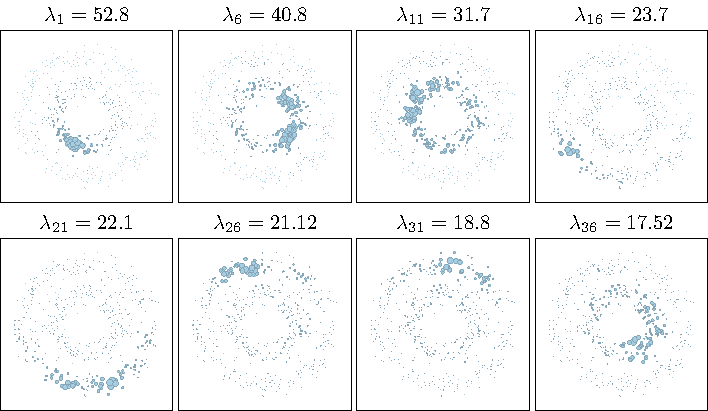
\includegraphics[width=\linewidth]{pics/SAProjEigen.pdf}
%\documentclass[preview=true]{standalone}
\usepackage{amsmath,amssymb,nicefrac,bbm}
\usepackage{pdfathesis}
\usepackage{etex}
\usepackage{xcolor}
\usepackage[a4paper,left=3.5cm,right=2.5cm,bottom=3.5cm,top=3cm]{geometry}
\usepackage[english]{babel}
\usepackage[round]{natbib}
\usepackage{graphicx,tikz}
\usetikzlibrary{matrix,decorations.pathreplacing, calc, positioning}
\usepackage{relsize} % mathlarger
%\usepackage{hyperref,url}
\usepackage{url}
\usepackage{silence}
\WarningFilter{latex}{Overwriting file}

\usepackage[colorinlistoftodos]{todonotes}
\reversemarginpar
\setlength{\marginparwidth}{3.1cm}
% Theorem-Umgebungen
%\usepackage[amsmath,thmmarks]{ntheorem}
\usepackage{amsthm}
\usepackage{thmtools, thm-restate}
\usepackage{algorithm,algpseudocode}
\algnewcommand{\IIf}[1]{\State\algorithmicif\ #1\ \algorithmicthen}
\algnewcommand{\EndIIf}{\unskip\ \algorithmicend\ \algorithmicif}

\usepackage{enumerate}
\usepackage{booktabs,multirow,adjustbox}
\usepackage[font=small,labelfont=bf]{caption}
\usepackage{subfigure}
\usepackage{pgfplots,filecontents,pgfplotstable}
\usepgfplotslibrary{groupplots}
\pgfplotsset{compat=1.14}
\pgfplotsset{
cohStyle/.style={ctrust,mark options ={ctrust},mark repeat={4}, ultra thick, error bars/.cd,y dir = both, y explicit},
densStyle/.style={cdens,dashed,mark options ={cdens},mark repeat={4}, ultra thick, error bars/.cd,y dir = both, y explicit},
primpStyle/.style={cPrimp,dashed,mark=triangle*,mark options ={cPrimp},mark repeat={3}, ultra thick, error bars/.cd,y dir = both, y explicit},
panStyle/.style={cPan,dashed,mark options ={cPan},mark repeat={3}, ultra thick, error bars/.cd,y dir = both, y explicit},
specStyle/.style={cSpec,mark options ={cSpec},mark repeat={4}, thick, error bars/.cd,y dir = both, y explicit},
specLStyle/.style={cSpecL,mark options ={cSpecL},mark repeat={4}, thick, error bars/.cd,y dir = both, y explicit},
RSCStyle/.style={cRSC,dashed,mark=triangle*,mark options ={cRSC},mark repeat={3}, thick, error bars/.cd,y dir = both, y explicit},
SCStyle/.style={cSC,dashed,mark options ={cSC},mark repeat={3}, thick, error bars/.cd,y dir = both, y explicit},
DBSCANStyle/.style={cDBSCAN,dashed,mark options ={cDBSCAN},mark repeat={3}, thick, error bars/.cd,y dir = both, y explicit},
clusterScatterStyle/.style={scatter/classes={1={cSpecL}, 2={cRSC}, 0={cDBSCAN}, -1={white}},
    scatter, only marks, mark size =0.3, scatter src=explicit symbolic},
nonnegScatterStyle/.style={scatter, only marks, fill=cSpec, scatter src=explicit,
     	visualization depends on ={\thisrow{z} \as \perpointmarksize},
     scatter/@pre marker code/.append style={/tikz/mark size=1.5*\perpointmarksize}},
pandaStyle/.style={cPanda,dashed,mark options ={cPanda},mark repeat={3}, ultra thick, error bars/.cd,y dir = both, y explicit},
punkStyle/.style={cPunk,mark options ={cPunk},mark repeat={3}, thick, error bars/.cd,y dir = both, y explicit},
dbssl1Style/.style={cDBSSL1,dashed,mark options ={cDBSSL1},mark=triangle,mark repeat={3}, thick, error bars/.cd,y dir = both, y explicit},
dbssl2Style/.style={cDBSSL2,dashed,mark options ={cDBSSL2},mark=diamond,mark repeat={3}, thick, error bars/.cd,y dir = both, y explicit},
mdlDbsslStyle/.style={cMDLDBSSL,dashed,mark=star,mark options ={cMDLDBSSL},mark repeat={3}, thick, error bars/.cd,y dir = both, y explicit},
% color change for embedding visualization (fuzzy clusters) 
colormap={test}{[2pt]
    rgb255=(166,206,227);
    rgb255=(166,206,227);
},
}

\Title{ A Mathematical Theory of Making Hard Decisions:
Model Selection and Robustness of Matrix Factorization with Binary
Constraints}

%List of Symbols
\usepackage{nomencl}
\makenomenclature


%\usepackage{color}
\definecolor{col1}{RGB}{166,206,227}
\definecolor{col2}{RGB}{31,120,180}
\definecolor{col3}{RGB}{178,223,138}
\definecolor{col4}{RGB}{51,160,44}
\definecolor{col5}{RGB}{251,154,153}
\definecolor{col6}{RGB}{227,26,28}

\definecolor{cdens}{named}{col1}
\definecolor{ctrust}{named}{col2}
\definecolor{cPrimp}{named}{col3}
\definecolor{cPan}{named}{col4}
\definecolor{cPanda}{named}{col5}
\definecolor{cNassau}{named}{col6}
\definecolor{cMdl4bmf}{named}{col1}


%
\definecolor{cSpec}{named}{col1}
\definecolor{cSpecL}{named}{col2}
\definecolor{cRSC}{named}{col3}
\definecolor{cSC}{named}{col4}
\definecolor{cDBSCAN}{named}{col5}

%
\definecolor{cPunk}{named}{col1}
\definecolor{cDBSSL1}{named}{col2}
\definecolor{cDBSSL2}{named}{col4}
\definecolor{cMDLDBSSL}{named}{col5}
% Theorem-Optionen %
%\theoremseparator{.}
%\newenvironment{proof}{\par\noindent{\textit{ Proof}\ }}{\hfill\qed\\[2mm]}
\theoremstyle{plain}
%\theoremheaderfont{\moon}
%\newcommand{\BlackBox}{\rule{1.5ex}{1.5ex}}  % end of proof
%
\newtheorem{theorem}{Theorem}[chapter]
\newtheorem{corollary}[theorem]{Corollary}
\newtheorem{observation}[theorem]{Observation}
\newtheorem{lemma}[theorem]{Lemma}
%\theorembodyfont{\upshape}
\theoremstyle{definition}
\newtheorem{definition}[theorem]{Definition}
\newtheorem{algSpec}{Algorithm Specification}
\newtheorem*{remark}{Remark}
\newtheorem*{example}{Example}
\newtheorem*{problem}{Problem}

%Operators/Commands
\DeclareMathOperator*{\argmin}{arg\,min}
\DeclareMathOperator*{\argmax}{arg\,max}
\DeclareMathOperator*{\freq}{freq}
\DeclareMathOperator*{\cov}{cov}
\DeclareMathOperator*{\anc}{anc}
\DeclareMathOperator*{\supp}{supp}
\DeclareMathOperator*{\minsup}{minsup}
\DeclareMathOperator*{\tr}{tr}
\DeclareMathOperator*{\bigO}{\mathcal{O}}
\DeclareMathOperator{\diag}{diag}
\DeclareMathOperator{\prox}{prox}
\DeclareMathOperator{\pre}{pre}
\DeclareMathOperator{\rec}{rec}
\newcommand{\Ya}{Y_{\mathcal{J}_a\cdot}}
\newcommand{\Va}{{V_a}}
\newcommand{\Da}{D_{\mathcal{J}_a\cdot}}
\newcommand{\KL}{Kurdyka-{\L}ojasiewicz }
\newcommand{\LXU}{\mathcal{L}}
\newcommand{\F}{\mathcal{F}}
\newcommand{\N}{\mathbb{N}}
\newcommand{\R}{\mathbb{R}}
\newcommand{\estU}{\widetilde{U}_{\widehat{CT}}}
\newcommand{\estu}{\tilde{u}_{\widehat{CT}}}
\newcommand{\estCT}{\widehat{CT}}
\newcommand{\node}{\mathfrak{n}}
\newcommand{\leaf}{\mathfrak{t}}
\newcommand{\krimp}{\textsc{Krimp} }
\newcommand{\shrimp}{\textsc{SHrimp} }
\newcommand{\slim}{\textsc{Slim} }

\makeatletter

\pgfplotstableset{
    zero color/.initial=white,
    zero color/.get=\zerocol,
    zero color/.store in=\zerocol,
    one color/.initial=red,
    one color/.get=\onecol,
    one color/.store in=\onecol,
    color cells/.style={
        every head row/.style={output empty row},
        string type,
        postproc cell content/.code={%
           \pgfkeysalso{@cell content=\rule{0cm}{2.4ex}\cellcolor{\zerocol}
           \pgfmathtruncatemacro\number{int(##1)}
           \ifnum\number>100\cellcolor{\onecol!50!black}
           \else \ifnum\number>0\cellcolor{\onecol!##1}\fi\fi}%
        },
        columns/x/.style={
            column name={},
            postproc cell content/.code={}
        }
    }
}
\makeatother

\makeatletter
\newcommand\footnoteref[1]{\protected@xdef\@thefnmark{\ref{#1}}\@footnotemark}
\makeatother

\makeatletter
%\renewcommand{\@chapapp}{}% Not necessary...
\newenvironment{chapquote}[2][2em]
  {\setlength{\@tempdima}{#1}%
   \def\chapquote@author{#2}%
   \parshape 1 \@tempdima \dimexpr\textwidth-2\@tempdima\relax%
   \itshape}
  {\par\normalfont\hfill--\ \chapquote@author\hspace*{\@tempdima}\par\bigskip}
\makeatother

%Thicker bar
\makeatletter
\newcommand{\thickbar}{\mathpalette\@thickbar}
\newcommand{\@thickbar}[2]{{#1\mkern1.5mu\vbox{
  \sbox\z@{$#1\mkern-1.5mu#2\mkern-1.5mu$}%
  \sbox\tw@{$#1\overline{#2}$}%
  \dimen@=\dimexpr\ht\tw@-\ht\z@-.8\p@\relax
  \hrule\@height.8\p@ % adjust for the desired rule thickness
  \vskip\dimen@
  \box\z@}\mkern1.5mu}
}
\makeatother

%----------box---------------
\usepackage[many]{tcolorbox}
\tcbset{
  myhlight/.style={
    colback=cyan!10,
    arc=0pt,
    outer arc=0pt,
    boxrule=0pt,
    top=2pt,
    bottom=2pt,
    left=2pt,
    right=2pt,
  },
  highlight math style={myhlight},
  mybx/.style={
    colback=white,
    arc=0pt,
    outer arc=0pt,
    boxrule=1pt,
    top=2pt,
    bottom=2pt,
    left=2pt,
    right=2pt,
  }
}

\newtcolorbox{mybox}{
	boxsep=1pt,
  	breakable,
  	mybx
}


% Zeilenabstand einstellen %
\renewcommand{\baselinestretch}{1}
% Floating-Umgebungen anpassen %
\renewcommand{\topfraction}{1.0}
\renewcommand{\bottomfraction}{1.0}
\renewcommand{\floatpagefraction}{1.0}
\renewcommand{\dblfloatpagefraction}{1.0}

% Leere Seite ohne Seitennummer, naechste Seite rechts
\newcommand{\blankpage}{
 \clearpage{\pagestyle{empty}\cleardoublepage}
}

% Keine einzelnen Zeilen beim Anfang eines Abschnitts (Schusterjungen)
\clubpenalty = 10000
% Keine einzelnen Zeilen am Ende eines Abschnitts (Hurenkinder)
\widowpenalty = 10000 \displaywidowpenalty = 10000
% EOF
%
\begin{document}
%
\begin{filecontents}{circlesV1.dat}
x y z
-1.0583288758102631	-0.20196401315764936	687976759029136e-21
-1.0549650952895588	-0.1453486277315127	7386196123201584e-22
-0.28686705420107594	-0.20577169621106567	0.17815435844407024
-0.22438385123724203	-0.6311838265132071	0.21592100451587828
-0.016329900725535695	0.8363156387087571	2674319214850201e-21
0.6664943110916062	-0.02522611869462293	0.0005527513587903361
-0.7000695186307817	0.8524609054729188	29529351835749036e-23
0.8737756445548316	-0.34343872237549916	3709281555963715e-22
0.26863712824940233	0.621230160725688	9076753978737366e-20
0.4135070890114797	-0.23094514442380681	0.00601075192492206
-0.8374130044011527	0.6731231597212262	17538278472700352e-23
0.6029899953791354	0.5490490339208243	9952071219487522e-22
-0.07532043439212403	0.4864515282258869	0.002931357139329265
0.38404755622047315	0.42223071846853666	9698024916316254e-20
0.5552969916156367	-0.1083120535732651	0.0018297134498240007
-0.21526850262358294	-0.49881387813462996	0.8946943548726807
0.0005701763274310358	-0.8608567301737946	0.00010661858325044138
0.5659515908300676	-0.16181812669682585	0.001850114873467643
0.7402734062213887	-0.7200478091020212	4925783986675728e-22
1.1196812938139424	0.34846871970260435	1596396947341649e-24
0.9436364508675184	-0.27253854831430324	5314624951671693e-22
-0.24546029448781795	-0.4906102105866899	0.78763669818148
-0.5666890574615214	0.8469922677428234	6202036475449384e-22
-0.8121420956043262	0.04089898834206568	0.00015379010534739392
0.6925296824873941	0.5004844069787805	973304360974059e-22
-0.7802845097289287	0.6503350319668115	5576970993205807e-22
0.19540149773912174	0.9988933466475728	24443428756964744e-24
-0.49033960699830575	-0.745615965610353	29325642970168703e-21
-0.772379045803115	-0.5555503478357138	24660986207932743e-21
0.08949600849053171	0.43569426601040284	0.0006895437731731368
-0.2709014254935288	0.8329314883710439	1858667573484484e-21
-0.4724968520274526	0.39757762314794287	0.01400469907519787
-0.05076606623229138	0.9472731081345089	4849786056715719e-22
-0.4244181110366452	0.15163647468601898	0.05710547728093898
-0.856823736320482	0.42050645578658474	1940309304990451e-21
0.3801522274867655	-0.5242396510380898	0.01085602302957319
0.5302560693756595	-0.046308947018418645	0.002341799906206716
-0.0592471029661714	-0.8742925870679111	0.00010851122957934113
0.9136426992044209	-0.6268351541350334	3780614075344911e-23
-0.8755978758264108	0.47329951242226026	5595983976092128e-22
-0.4611459366222198	-0.29641002189383403	0.26089658989048303
-0.037954030937970715	-0.5674223028442248	0.515173242934422
-0.2144341080960731	-0.940890046876266	25292234206844616e-22
-0.15386158302832836	0.8539796415576204	4019652964257018e-21
-0.34600659981207815	0.22605644970598238	0.04294469927408564
-0.5581576930234105	-0.014719460229306036	0.0365112394640575
-0.8197754374675081	0.717359733882507	24995078415116687e-23
0.27775250685348385	0.18189032091007415	0.0003456898491932029
-0.4029746673951193	0.1027363359902787	0.054062044575186104
0.4968916538935379	-0.000844611354336014	0.0020705980157979553
-1.0774087697285004	-0.07678224474566575	6851299550051645e-22
0.8614353478008437	0.025271734377208227	13743177148474474e-22
-0.801406799115663	0.5601142307444397	486585993725284e-21
-0.4793204129385923	0.3306162943293071	0.031592207237906685
-0.6015487302066529	0.1320612905764609	0.023855541942386475
0.5617427965558156	-1.0113021326424354	3102206428439462e-22
0.730444208221491	-0.6768972250254602	79721244503304e-20
0.5214794214363629	-0.5008727775322623	0.000616275463520605
-0.07937288077704525	-1.0020594043483257	29665956424782087e-22
-0.4105200259369002	-0.863231624107107	5087349582846109e-21
0.3388762765570134	0.08706717470919467	0.000800695098908496
-0.8685030533130447	0.3738037066733266	2135906788251181e-21
-0.45683545912363355	-0.04267855156658711	0.05025966850123004
0.7512915187942618	-0.643291765899665	7172604804742435e-22
0.6216335172514909	-0.11511316015280951	0.0009571941646840217
0.2989142354739267	0.39780163534212587	0.0001476829361261019
0.8832260533811114	0.5378029603982082	1479687188643962e-23
0.7706147096701259	-0.5688688999070458	4262228438259068e-22
0.7777354887198962	0.720528533564723	4310908190388121e-24
0.33650550115674555	-1.115393724949389	2290487646665865e-22
-0.342570290724111	-0.21142060265518764	0.22021156641099834
-0.25812602086366604	-0.36207505076781854	0.8291244748424244
-0.440512439401967	0.41982647549444946	0.01356126625467441
-0.41029305865551974	0.5613483829060184	0.0023760934755905102
-0.5385119865491543	0.854068737227722	46804921608284784e-23
0.28817771225733035	-0.35555608208892875	0.02114774704461659
-0.46394391030820226	0.9413388577320934	3035129735682728e-22
-0.24831840720533802	0.5237809077418585	0.00435086555720168
-0.6552850605832186	-0.4599331054248453	0.00026446562713125705
-0.2826163494076298	-0.9757361666246253	6395291442346341e-22
-0.3774044986295204	-0.15754990126458723	0.1718272412396457
0.39289772381826926	0.21639482757710704	0.000545843947319971
-0.3000684974285963	-0.9288792097716005	999220901377361e-21
0.23230106715972593	0.5053020150438099	0.00022389340314926402
0.035704278426334946	0.533270659937437	0.0011356479147815724
0.09598775875172952	0.8618425666792344	3289196704723673e-22
-0.17962630292512827	0.5212494227356729	0.004244832384434762
0.31236804409574365	-0.34388834400933016	0.02173315701702628
-0.47976322944270716	-0.5787808073254304	0.019263259308459565
0.6093508783156708	-0.6552395783902365	46348541971280825e-22
0.8464430922888276	-0.6582476883085377	14449881885219646e-23
0.30952844675119945	-0.30050993673209625	0.012161864593158473
-0.35579373024330907	-0.3031730669351904	0.4458458843024813
-0.4729710467200588	-0.9161905551389896	36764422000724584e-22
0.8105489062223111	0.3063890203748192	4228985253439654e-22
0.26349519971405094	0.3154986373224412	0.00018491240430886226
0.151915912568039	0.5325519003756559	0.0004903229320341736
-0.10319754741500724	0.5493951282610205	0.002520222749767573
0.9203553330570633	-0.29254729468906093	544644299707871e-21
0.4831799702244233	0.060377797979320996	0.0016944222991926773
-0.5796183887393597	0.7746200654923161	11511741541783402e-22
-0.8541885431589489	0.5178310337137458	5635530289048223e-22
-0.8796583444738513	0.7081111554312315	6249669180532147e-23
0.34083406290250495	0.74696794539091	35780357527016524e-22
0.6438062065547421	0.684737062537711	4602542477738397e-23
0.8167936695881719	-0.7568243617688544	1396508794667108e-22
0.4246697255417251	-0.3328124636208833	0.008137675043241316
-0.9859854354757545	0.26344939470473255	8783425379292635e-22
0.36302398095734684	0.2746590061351894	0.0003293231807867095
-0.025297734684784023	-1.143907353283561	19392146342097465e-23
0.2032554345955354	0.28830564392732866	0.0001767967276239974
-0.2502433512821886	-0.41755435063352553	0.8595418664544406
0.5098578452924067	0.4695047239790404	22089329689357823e-21
0.3443787337008237	-0.4675382901965091	0.023181377978022166
0.9881522604297938	-0.3021471510603488	17056016447195702e-23
-0.48057110152907556	0.057853088635956826	0.05312845903214104
-0.1494073465765274	-0.4744536378002139	0.9763040372169911
0.2291058540766086	0.6877816124566098	3105363401895568e-20
0.10432827601608814	1.007003579269503	6085989839492026e-23
0.031436823141421995	-0.3070447159882047	0.04152011647189512
-1.0941411050076675	0.3821308374739647	10485243622358463e-23
-0.006772415554554288	-0.3403823630501911	0.16983310846608035
0.03790459976473807	0.8981000637907597	35311524580968386e-23
0.4724071282898181	0.3379026545362105	0.00011841588859968858
-0.5687164572253783	0.11499339914612097	0.03221656236486325
-0.08693938008162763	0.42279389507717124	0.0032787064363513376
-0.28689351236975014	-0.37462850605791104	0.7534021056043091
0.8626364254896491	0.3878238798233949	8184937491350128e-23
0.2454241460431366	0.29822889729914215	0.00018359719026852524
-1.1331872257168936	-0.014302927588677045	4201528432229772e-22
0.4474309277283363	0.15150716280611207	0.0010735944019490083
-0.9952111212193668	-0.2692696791591609	385953350634431e-20
0.33451824342581943	0.22445047758195008	0.00039345008517963174
-0.45141735558253765	-0.5264915335380573	0.06342766350799213
0.14051117817071368	-0.9453552208299545	13285816599531553e-22
-0.5491877812265945	-0.801112192863598	29481655633360168e-21
-0.9863368691505784	0.41417098820521786	440638274728957e-21
0.27278308023328324	0.8296836984169661	11197993566709313e-22
0.1891406899596204	-0.27355388028025107	0.012542774385133898
0.5534652549685908	-0.5958867421206311	58519086256949506e-21
0.6847207172590709	0.5463728715139321	6590444860887072e-23
-0.37443413523697894	0.8760256040266927	43363477961552595e-23
0.4392548163834803	-0.9047561020319701	4053222477195189e-21
-0.19545855718707983	0.3152184994865719	0.005379575921434386
-0.9941933253410392	-0.3165529558686342	2884762905638684e-21
0.90768322436734	-0.39962363443787496	10116057802616773e-23
0.21606973625964263	0.537937900067448	0.00023694358612409401
0.17926414498256826	-1.0625373062111834	3698747480520882e-22
-0.3842822926705394	0.07890580561977101	0.04717942274259274
0.9483542004901386	-0.35261244440864314	1238497825929383e-22
0.4937510937461273	-0.7512057092701449	15807309382772896e-21
0.002194023717617566	-0.9067718398812545	927952450666516e-20
0.04853172316213811	0.47150668085564584	0.0010778721229098935
0.058687648748172734	0.5599084359157949	0.0008889804752103101
-0.5342332606475368	-0.07309364796671353	0.04791367456264743
0.9166764532207246	-0.17096965575209683	962543774948631e-21
0.5560622463214425	-0.19500798744869144	0.0020726469919232294
-0.4508337971767867	-0.27343096232028685	0.2866015935145675
-0.2249770521470013	-0.977120879775083	6113584380321109e-22
0.5105063250464269	0.17053921152739293	0.0008519259455008477
0.22610688378803662	-0.9577438670294672	9667542071847555e-22
0.7003486506302466	-0.15180173128212845	0.00017500360464815088
0.006636214456188352	-1.054807062255213	9673044514861463e-22
0.2584532151158738	0.9829378520319795	3397965978994049e-23
-0.4557941617257688	-0.24674411027449922	0.2333426179815954
0.7116187117871964	0.37399667612376497	42914279469372275e-23
0.44253310209306695	0.9491491060163105	22845097353449053e-24
0.08447685192909979	-0.8351535915539824	8863881369857815e-21
0.5633797515703941	0.7560384738182708	2287815571356609e-23
-0.9683305242013036	-0.5729099853696185	31171470747517634e-22
-0.5127125337250293	0.8022392827607193	5712020073187479e-22
-0.4025752704584875	-0.19586338037814632	0.2062791591580176
-0.373579961679699	0.07076226765469532	0.04549910227224119
0.5847086359226571	-0.10428584342601002	0.0016052238979785368
-1.070192755078586	-0.5175893695396888	25086075757722183e-23
-0.37585788050259117	0.26622981099006604	0.047481323865519655
-0.04153066411364073	1.1298070647975962	7820480026369863e-24
-0.29849855076934684	-0.439235662946394	0.7611457024134005
0.7986762407696741	-0.12350308057782419	21420021396020292e-21
0.7241725359210982	0.7673470713309014	4154611593008038e-24
0.4425716175145471	1.0545877925203901	4517520327075642e-24
-0.3009942479406195	-0.28544465808629016	0.4287049418161772
0.28456936812944295	-0.3657137258550358	0.02178806099028045
0.28744578929175285	0.32854425576712576	0.00020631417959207136
0.639937762556447	-0.6505099028952075	45842621664898e-19
0.05823208873356708	0.9054436486403517	3546041876317958e-22
-0.18827083294877459	-0.5175564452077821	0.9108231492033209
-0.9329068382156008	-0.3801321106596237	7599034298521216e-21
0.5601450967893756	0.09698845485225183	0.0011501551043251112
-0.3756527474612627	0.7120960532866892	33185441842445497e-22
0.28648170510331256	0.3442269536180647	0.0001816900204669042
-0.5545045803725894	-0.854004082386823	21986593367885936e-21
0.27939838551695295	0.20316442364718562	0.0003159342689058843
0.16904383170478116	1.1363146779633637	3818200530662629e-24
0.41960093047149866	0.13705185266873904	0.0011431353965622292
-0.4498033980116379	0.22672303751202222	0.05392730270001006
-0.5081276724502488	0.11652282996013652	0.0507943901058836
-0.04972504364164415	0.31835178586661395	0.0009590992975685355
0.5272444182086248	-0.7879070986907416	35335175549696355e-22
-1.0654861621254115	-0.23509318286565328	6635511712047088e-22
-0.9887302337932489	0.1103754459557201	26500360503268926e-22
-0.37771282161869674	0.2089104993471779	0.050017634593180246
-0.592996935730106	-0.11660158192407682	0.023890116357875843
0.7777222354165501	0.5099416601581699	4396283823693886e-23
-0.6597553949317734	-0.01980472153961566	0.008471011535055478
-0.20893659613357207	-0.48724539646942766	0.9093488753578578
-0.8068455521466513	-0.29997047342039707	0.00018838146789521966
-0.6900745319305372	-0.6280428506278541	16848631006253368e-21
0.8614051450394694	0.267928431998897	40055656222127127e-23
0.5913328927145274	0.7855026465857798	18151196036025133e-24
-0.9217563671575004	0.24534492193834448	51211060882629775e-22
0.38474371433279925	1.0935616549059102	11715554962536724e-25
-0.46741030056521377	0.2591755254370145	0.047260072251211815
-0.0381025675995942	-1.1251543679349862	37290299289886735e-23
-0.6243967254451009	0.46517409634094015	0.0004450085339160657
0.21707179540902807	-1.0140863576742312	5613798829727398e-22
0.7081813705522666	0.7162885127966534	9815410449997586e-24
-0.9451644776861263	0.18394464444693226	675828659555267e-20
0.3729334539383104	0.46088009666634666	6615299130200575e-20
1.0696979889031235	-0.0794841459498074	3932366594472406e-23
0.7555529047587174	-0.6789645529590862	7509897735164391e-22
-0.4390917083090098	-0.2160668681154164	0.1919587106072599
-0.9161126914457096	0.5398116209231641	2355536972473724e-22
-0.7407788219528375	0.33551254951641335	6814936689742698e-20
-0.2114261856758002	0.8187152036533841	9754638719501758e-21
0.701545668282712	0.08200865693028041	0.00014349153405292093
0.033338468862882234	0.6199041811295294	0.0006183926814249463
1.0748984302382512	0.35907777637212224	24252781344128707e-25
-0.4597850556976463	0.045223030444219284	0.05378463338264669
-0.1741463993378947	0.7865778186239607	2076249229881262e-20
-0.33728863860345176	-0.35849990456630876	0.5715513853651248
-0.9587665698372234	-0.42543103080047867	4982111203084549e-21
0.2123157690598867	-0.9860875988345833	9943151121386175e-22
0.04602382173605105	0.9088619887209635	35689148418546146e-23
0.3725537615240344	0.1876685667278354	0.0005323993176489865
-0.8740700379235082	0.31983625072337724	394396413912705e-20
-0.3892066741361861	-0.9811247119391876	9022825157028842e-22
-0.8474412504983133	0.4654098218172844	621389379436518e-21
-0.5108698639619283	-0.10057435621987655	0.07469706863746083
-1.129071205600398	-0.17027012619747586	31562111412901e-20
-0.39514507247834857	-0.8103936481837801	18745432055901755e-21
0.4704996641617121	-0.17220690970158825	0.003556735352217171
-0.37983945734932445	0.12041154024224539	0.051664067678708306
-0.055472740425509856	0.6206042795137554	0.0008418593987128163
0.3645979153047041	-0.41706786292712994	0.016175952871092067
-0.015561824056395212	0.8198043684673366	9080030140413172e-21
-0.44145592026764	-0.2505282912308723	0.25369889110765625
-0.2561401471320713	-0.40112951606947655	0.868624467749652
-0.52338679166547	0.02660578819265639	0.04203722911495992
0.21445818450520165	0.22082326083082776	0.00012745893534484232
1.077569058206745	-0.3491332068383815	24294410367272213e-24
-0.1872746787626816	0.7899535223817675	20784101599586684e-21
0.290127993873019	0.8394507724623782	5433619158280008e-22
-0.8865250322253393	-0.08940312375709093	12815819843474678e-21
0.8621507749457712	-0.34819857547136623	33691481252205987e-23
0.18225473918119706	-0.28728382873787084	0.016627101983279553
0.4654196763131379	0.8563057194157547	35354340194794333e-24
0.8303630898153743	0.36063100311212853	4261839446174578e-22
-0.9712638110423526	0.6382288332737301	4610470515973026e-23
0.23666688614920567	-0.45266804798952437	0.04883570289213089
0.6309050357598261	0.7240590312014205	2189050024184943e-23
-0.42767689370476714	0.9491438031378565	27959047081350044e-23
0.44563927184415986	-0.2274601203045902	0.004055105894582521
-0.2053874739053867	0.4253844412184107	0.006999073334742131
0.5405420315871583	-0.15236975471038613	0.002264857191687393
-0.26241022071698467	-0.4527201725965245	0.8259953110261454
0.3800831916990306	0.7125239676567952	2747050491258512e-21
-0.5746742466560214	-0.14252620560541895	0.05383982994058495
-0.353711250098192	-0.089227175639014	0.07191632903369924
0.9454568469815224	-0.6882256956905914	18858202044905343e-24
0.8557340217873753	-0.6560332493577736	12413542577632616e-23
-0.556562516437247	0.025216778123066684	0.029636692173030495
0.636271359519193	-0.1412312507678136	0.0008490835190640259
0.45228206748941496	-0.1464962121039572	0.0038779608259858407
0.29958240361829125	0.21950393236552065	0.00032678724139989447
-0.48441555279257537	0.9138234923246589	36988856457648106e-23
-0.4461707440833614	0.9247836035865585	33862623315730784e-23
-0.4201939672191152	0.147701646190593	0.056219461075248264
-0.6425112593179262	0.8853425199869299	29945495045399257e-23
-0.9942338743953323	0.29442352385918036	8801715505268484e-22
0.5984091164639631	0.6507722124429921	714916688724187e-22
-0.44739056708622243	-0.19530513215445594	0.18594593894638917
0.10544312980633214	-0.8886995454263548	7148358125200326e-21
-0.16519124887174855	-0.45974106532199166	1
-0.1452578553741265	0.16491959057663946	3047328413428026e-20
-0.3271832988321618	0.15469783349016974	0.03858780214821989
-0.11311105980459281	0.9135157952010174	18548674626427548e-22
-0.3561083380389497	-0.2947817783686462	0.43490223268456263
0.3724658234027415	-0.9915409863714767	19093619049110764e-22
-0.809763642248029	-0.12327687501896292	0.000205460495855068
-1.1287681161906478	0.06262847595617371	4447570461916485e-22
-0.6997744034861316	-0.5562715236294364	321238374472271e-19
-0.686767025909816	0.22799527222288463	0.0032908344832878376
0.718150173365836	0.614101346547797	4810628078802753e-23
-0.45660502262193225	0.30925490188894406	0.03654263012800704
0.5685590020433319	-0.7691628640835012	37089941523937966e-22
-0.21120482990041983	0.8920372566221498	19091548390033314e-22
-0.8559997833581601	-0.10979459128678692	28031286631626762e-21
0.020241236020441977	-0.9871905648513019	5233264691499702e-21
-0.19378550438170256	0.529549096346015	0.004189846077931001
-0.48576133985104347	-0.7248762853196216	0.0003870570902795034
0.39513367611481626	-0.8885158369058909	4013030238357137e-21
-0.18721242838064622	0.9702879441616987	4061731354601975e-22
0.8396921444402687	0.3365818412168194	4257295193632143e-22
0.877467440180306	0.39080964030788956	8163289024795694e-23
-0.5499282479717139	0.5999930092507813	0.0002453651908515492
0.39606976564711266	0.01353375952124733	0.001921175892101656
0.9408685147764327	-0.16839212966354405	927685777895485e-21
0.058529813294819356	0.5960832480212296	0.0006970806883852174
-0.3085264124619913	0.867923991978884	11630369001701663e-22
1.0240606495199067	-0.05902106596557902	5743996584054494e-23
-1.1297448788625983	-0.08852295833376425	31474134293741186e-23
-0.3019985141368995	0.30893831800591814	0.02148092657522364
-0.008533740271034915	0.8593779967999691	26743192148506146e-22
-0.47766065242119404	0.09174102825933139	0.053326782742638565
0.552796931763394	-0.07589565750634704	0.001794377375019225
0.603572742486676	-0.6831181382142064	27953295513778685e-22
-0.33288992349487256	0.13169527999030434	0.0381908937319041
-0.2390174716089229	0.7900359421455263	9678838125683676e-21
0.5308565325208349	0.507359333449821	14512120551653933e-22
-0.24541435549726867	0.2808122025738658	0.012972853067883563
-0.29898976544354733	-0.7827067523032034	23205358915273614e-22
-0.9999570201344817	-0.2026055094073493	19218286705388836e-22
0.29758558346109265	-0.36715492999328203	0.022011315054850197
0.8674564090945402	-0.5819678100623382	7300557334568551e-23
0.600229072467383	0.22647599269832278	0.0002640674878813101
0.20769676592782566	-0.2429673540455613	0.009091238993045177
-0.16980961206235062	0.44328283958495246	0.0056152346685033865
1.0742084655937019	-0.026185528019472687	2395117173137954e-23
-0.5990364456171003	-0.025393658161253316	0.023284081960375434
0.38651874675910325	-0.0313701916023475	0.0020250973270705226
0.5347630915993977	0.17166579010558058	0.0006803294001614598
0.3815611790828055	-0.15397406983635387	0.003539563791397765
0.5058927256985234	0.23791877175557427	0.000445429448111775
0.7572842422665051	-0.7254577812166593	2711129700603262e-22
-0.9360697829922907	-0.35462224573950774	8446580525728072e-21
-0.14478358844783776	-0.9498460059976374	4599607947932434e-21
-1.0228407301441125	-0.0018387135408612018	18337106716486614e-22
-0.8185514119556835	-0.5782789864229126	25249665647817257e-21
-0.5190222237533468	-0.14121284297452863	0.1028600154750412
-0.8812420477325542	0.09550201023389113	40016075000964435e-21
0.8043770929313652	-0.3853011709405064	7844353685356873e-23
-0.03568713716803138	0.5775112808391898	0.001052068480834077
0.35582627317999016	-0.23527882041840337	0.007848792361647905
0.07420419694257939	-0.9294188883144827	936455577470905e-20
0.1662899576554404	-0.5284808316844934	0.11435967878366314
-0.3572795738981698	0.8443053913527945	8495652087924456e-22
-0.9577523664409258	-0.29415179908865413	38797365753035585e-22
0.4986549895301416	0.7233237313187797	18215251804223754e-23
0.11984529006189726	0.4304757087557079	0.0006430562344810005
0.677209428557069	-0.1968148144685232	0.00025867260699753323
0.353158843408339	-0.2294141726153695	0.007333860472072097
0.6926163091663033	0.9082438486259222	13305959399929301e-25
0.22662062842571284	0.7101939697778475	20075135248296205e-21
-0.6173942947547322	0.6857369967943334	12522140833141256e-21
0.9361950579940088	-0.5613127488775519	23371465170677977e-24
-0.127424404632568	-0.4268659769339036	0.9470742298344268
0.26174039678270733	-0.21335055076531645	0.005052909852641206
-0.14895845969227897	0.6038885892071426	0.001210755093556201
0.017206819968116654	-0.5610869042333229	0.4492943805497979
-0.6165701158875304	0.8039827900466703	11415465984723164e-22
0.3368370747340216	-0.6011912237933033	0.007152403389712189
-0.004612791244162896	0.47514382808152794	0.0014565744474741944
0.01843812087421645	0.4484493986239611	0.0012451060806369604
1.0102123569818526	0.5165463334857523	3459898079000362e-24
0.7972873049177899	-0.3639915217251992	3108190296152853e-22
-1.0664272738526281	-0.0883863999456583	9867603922124017e-22
0.6426248444603162	0.14819452862153007	0.00029402028233657196
0.9008961948591205	-0.638870305850429	6164685718501925e-23
0.07864578043864236	0.4429924687743171	0.0007596960583895402
0.24736111985778403	-0.46837324136874914	0.047338771279151946
0.11571675991762002	-0.5488435993368718	0.1405660195860155
-0.25999785574842316	-0.4648227479797838	0.8171098552433961
-0.1282785387957175	0.8005039835738349	15054905229340922e-21
-0.6941747414267789	-0.10895464287467746	0.004312198405479585
0.5643296830461592	0.41564751900823327	2560482462376823e-20
0.393601640931545	0.8965530173420195	8683902061530899e-23
-0.6242684592992149	-0.68783187626963	2848182522711646e-20
0.4054686352399301	-0.33391817631930143	0.009547506139647546
-0.3861661312630557	-0.19434905522093565	0.2119605677175169
0.9141444978148033	-0.2052575568430186	9391185936522531e-22
0.2569409389934234	0.22066279246844922	0.00020733269874683412
-0.3406827094916554	0.3943071650929997	0.0183394286358125
0.44542838045587774	-0.9405066295787441	30110864746728865e-22
0.486743607490183	0.010295075115063876	0.0021404602577832807
0.02567392299065019	-0.5353718854477386	0.4483566618438325
-0.15396452356596207	-0.8301000411980569	0.00010398553884257198
-0.46406039285362755	-0.07011817763253647	0.07002335647420559
-0.1654591278460084	1.0093935572815773	2454795074912324e-22
-0.741574685169897	0.6075049586400391	1370569164644704e-21
-0.8839504856898732	0.4843707069263513	5493270439024073e-22
-0.2772708916507828	0.4271776286910839	0.01123446670264895
-0.007915654790254648	-1.0374245659643888	9900160936166507e-22
0.07158038113892838	-0.4470777829690491	0.2715891058495441
-1.0979023568400463	-0.2788707017013692	5614168785743902e-22
-0.8383403144319864	0.47642383134293137	5280280757576092e-22
0.6722758352720496	0.7407194847455977	1170497785388399e-23
-0.04462100192073412	1.0253515873635495	1231048760883581e-22
0.3059243103815058	0.30551382614764	0.00024254233462774998
-0.5007235364262262	0.305162592217073	0.03042068599887004
-0.04835433089425645	-1.032045099586184	8503059139984857e-22
0.5223335457063931	-0.8001425195591133	3549049014251947e-21
0.24149010192315168	-0.8715983385787441	27572129603612808e-22
-0.7942862878598648	0.7355786621547904	510020427863332e-21
-0.5840637350131117	0.35352633664496064	0.005379523945150776
0.7666697426076825	0.38792851703849934	4402781839135756e-22
0.3602768399720905	0.11065682747370947	0.0008846523870060412
-0.33762463156101746	-0.29981653068887726	0.46631415809517973
0.7413270931177445	-0.8012725814158732	16851719139909864e-23
0.41530854244488424	0.25140265746432494	0.00040768117063939846
0.34830580483963713	0.43593266031629013	9173828658035996e-20
0.4481077666063202	0.5022198174529555	219337324674145e-19
-0.07078374784853891	-0.46365027125240593	0.8370576560819322
0.40691344638633065	0.20194743468366066	0.0006157753406298368
0.26473797616138184	-0.37970123656838783	0.02726137508491243
-0.3430075566496395	-1.001014309078478	5630847162846604e-22
-0.07098190777517646	0.49124527294967674	0.0027048990383244167
-0.3696423277599601	0.9311821284465949	35858795735623594e-23
0.15781888335557667	-0.818076320322263	27798766320672534e-22
-0.012063147114350647	0.5015628247807506	0.001518508787955284
-0.5401592010556218	0.886425655241674	44736322079676597e-23
1.0143693052313847	-0.13847113343398026	12767918771486876e-23
0.5426832353988738	-0.028865776093147645	0.0019397705015600844
0.019493189988530002	-0.35211917974380724	0.1579499087200321
0.39796033385805474	-0.21653420832469542	0.005674400855326473
0.06932313386297567	-0.4650929980884387	0.33826381069191547
0.3855920910769304	-0.3703680740548607	0.01181400512001456
0.07668961878948749	0.504487350499383	0.0008379949952606556
-0.41590152051588525	-0.38590385766809937	0.3685038305946393
0.5112713182857704	0.300526008214048	0.00019970580190103307
0.44278962454753035	-0.12582498230716915	0.0037053577283125924
0.3587073438595803	-0.924707220336543	3895358939117396e-21
0.9819876679370327	-0.2645150004065293	17842828656976446e-23
0.042515674170929135	-0.7902031675276707	0.000106406537264838
0.9842189549691335	0.41115896420360276	15050140966378974e-24
-0.4339910269991673	0.15042822254012278	0.05849108155534333
-1.0664501738684824	0.05611953902551445	873346533665334e-21
0.12381363799397313	-0.2906794546712879	0.027010669548066864
-0.9287624426681778	0.2980361842691943	26256279163715315e-22
-0.32467663804828306	-0.37282219809450984	0.6203777003331049
-0.017267746630876546	0.30114051365578065	0.000543642719938363
-0.20322929100860568	0.34196259635971044	0.007093012344065527
0.6149295803569534	-0.6574878070065425	4569000422389517e-21
-0.5019331683517144	0.5034120088464493	0.002667478067261255
0.37959496422941374	-0.19817478772397484	0.004955023245102079
-0.6288413136352182	-0.0686225510329849	0.019160498081953005
0.5576922952499451	-0.7372777659850459	3834510157275666e-21
-0.7473156621355121	-0.35958003748297923	0.0002031576215397001
1.044766441941261	-0.1640132387701801	11056882933297713e-23
-0.5248584449224766	-0.1626584031102783	0.12558797543043734
0.5468339285697519	-0.8515486695216632	22604546595215726e-22
-0.8488608547924452	-0.5277291713396844	1896942884631836e-20
0.09129344106845708	-0.9929084269568997	10749879579513075e-22
-0.8133312932653112	-0.4325977063875221	34821546650800266e-21
0.42790218086737897	0.03368246917509174	0.0018544695110320197
-0.345703241038376	0.2669186991384062	0.03976606218036156
0.3743264449179663	-0.5437708269458819	0.01033215796419803
-0.771818816673675	-0.23721045607514987	0.00084048432996943
-0.9459166240312367	-0.5947562706827852	3610010714120574e-21
-0.4543408316958324	0.4716252527218408	0.00715106629933941
1.0190866335789526	0.3711877245816759	917414733506956e-23
-0.21781367160080423	-0.4364787637053435	0.9199098336426929
0.6694831669040802	0.16780314195860563	0.00022372796532751807
-0.11334332903498678	-0.30867673172262705	0.2643272881128332
-0.8479602054835725	0.5928559189151142	1952476625479501e-22
-1.0044694724664094	0.36164690812566047	5642233737966592e-22
-0.6964101427144668	-0.04329881702200409	0.004098582604578063
0.15553838290615063	-0.4545474031281862	0.12305900514671539
-0.6330956374343583	-0.8230604228089214	13339054795646677e-21
-0.834071330279343	0.5284489610165986	5404697472980327e-22
-0.7603398421567891	-0.3478439515517804	0.00019301927089352685
-0.14599715053105988	-0.41447742938148424	0.9368054283078172
0.7985840911794406	-0.8416644620776599	34257821649128504e-24
1.045546872577677	-0.32961473056675883	49426900900327206e-24
0.9216600778725588	0.19676141715944806	16546583973312568e-24
0.13536177018969225	-0.5654614405280538	0.1255426913994526
-0.1467968113274581	0.9327024933348684	15836906155103976e-22
0.8828512011106353	0.3995720345410485	8163289024786591e-23
-0.5250562446249011	0.9959137054261278	1354190720399071e-22
0.4444706003292941	-0.08613466876944118	0.0031763205215376124
-0.03651906329943556	-0.5776097455166717	0.4678789998948669
-0.18275922882623855	-0.36911929361528273	0.8181541060429669
-0.008357904929132312	-1.0400712136700585	9900160936166515e-22
-0.46490602896191124	-0.7521850939029222	2886200117989813e-20
-0.8629666931629013	0.5586407994356856	40959839211027205e-23
-0.6494376078685997	0.7979569864308408	10651357094365384e-22
0.8100743508008097	0.5222176894097934	4523046579280407e-23
-0.4763513992824499	0.29435036447461255	0.03905780080102962
0.9968051748529907	-0.2575222892887514	1644969149756686e-22
0.5242050451376069	0.8022664649393088	2682182210941204e-23
1.0537007610962097	0.04186827819127899	12989114043954501e-24
0.6866816563190805	-0.6998664005357831	12834126448337089e-22
-0.8686423707348288	-0.2343643483529707	54073642805727994e-21
-0.40482879492639007	0.3791464480343506	0.022123287344186702
-0.6514563822495386	-0.8843925992284258	4954530228030426e-21
-0.6751986838155158	0.6808714231615992	61764334561856435e-22
-0.17206390120164555	0.484188774179118	0.005101567851704851
-0.1777624864565969	-0.9108790982123965	4609330419878977e-21
0.4561691628917222	-0.29274091655163537	0.0050242086390658155
-0.31002924981632496	1.0304684380914757	13404659576895345e-23
\end{filecontents}
\begin{filecontents}{circlesV6.dat}
x y z
-1.0583288758102631	-0.20196401315764936	35197880937678706e-22
-1.0549650952895588	-0.1453486277315127	28050519493063334e-22
-0.28686705420107594	-0.20577169621106567	0.10669345358498881
-0.22438385123724203	-0.6311838265132071	0.043050907069448786
-0.016329900725535695	0.8363156387087571	0.00039159282448753913
0.6664943110916062	-0.02522611869462293	0.0211148303204303
-0.7000695186307817	0.8524609054729188	16086240934734547e-21
0.8737756445548316	-0.34343872237549916	0.00013223849566522202
0.26863712824940233	0.621230160725688	0.04106327999147528
0.4135070890114797	-0.23094514442380681	0.9393130971796583
-0.8374130044011527	0.6731231597212262	480534466492942e-20
0.6029899953791354	0.5490490339208243	0.003986486500322154
-0.07532043439212403	0.4864515282258869	0.2002084765955412
0.38404755622047315	0.42223071846853666	0.3491102788014534
0.5552969916156367	-0.1083120535732651	0.20875431551316478
-0.21526850262358294	-0.49881387813462996	0.12539005053130564
0.0005701763274310358	-0.8608567301737946	28871481080050225e-21
0.5659515908300676	-0.16181812669682585	0.34186816037816375
0.7402734062213887	-0.7200478091020212	669714541203161e-19
1.1196812938139424	0.34846871970260435	5089576340251399e-21
0.9436364508675184	-0.27253854831430324	0.0001780406737195089
-0.24546029448781795	-0.4906102105866899	0.10000299314113971
-0.5666890574615214	0.8469922677428234	42829729036076685e-21
-0.8121420956043262	0.04089898834206568	1767231348647794e-20
0.6925296824873941	0.5004844069787805	0.0004283694167204316
-0.7802845097289287	0.6503350319668115	13863565100575811e-21
0.19540149773912174	0.9988933466475728	5374163777566171e-21
-0.49033960699830575	-0.745615965610353	19023419512971332e-21
-0.772379045803115	-0.5555503478357138	59397152907110416e-21
0.08949600849053171	0.43569426601040284	0.07573689713963601
-0.2709014254935288	0.8329314883710439	0.0003369039827890958
-0.4724968520274526	0.39757762314794287	0.07500711738426828
-0.05076606623229138	0.9472731081345089	9311953073332507e-20
-0.4244181110366452	0.15163647468601898	0.10939769962763672
-0.856823736320482	0.42050645578658474	32562640590194833e-22
0.3801522274867655	-0.5242396510380898	0.31603712028646014
0.5302560693756595	-0.046308947018418645	0.04698604385172763
-0.0592471029661714	-0.8742925870679111	29673752595866268e-21
0.9136426992044209	-0.6268351541350334	9714023076836854e-21
-0.8755978758264108	0.47329951242226026	22535131112239694e-22
-0.4611459366222198	-0.29641002189383403	0.21542814424745932
-0.037954030937970715	-0.5674223028442248	0.04364482805235333
-0.2144341080960731	-0.940890046876266	6313681818393593e-22
-0.15386158302832836	0.8539796415576204	0.0006294698731113922
-0.34600659981207815	0.22605644970598238	0.027985365642134677
-0.5581576930234105	-0.014719460229306036	0.0008109861661365638
-0.8197754374675081	0.717359733882507	722015016177945e-20
0.27775250685348385	0.18189032091007415	0.6095535476559568
-0.4029746673951193	0.1027363359902787	0.10252651086860672
0.4968916538935379	-0.000844611354336014	0.11722252608887297
-1.0774087697285004	-0.07678224474566575	7137230388976721e-22
0.8614353478008437	0.025271734377208227	0.0003404439992537966
-0.801406799115663	0.5601142307444397	4872141231659214e-21
-0.4793204129385923	0.3306162943293071	0.03002599514564411
-0.6015487302066529	0.1320612905764609	0.05364866232629605
0.5617427965558156	-1.0113021326424354	11344038343265683e-21
0.730444208221491	-0.6768972250254602	0.00010382120959432349
0.5214794214363629	-0.5008727775322623	0.04272302932028465
-0.07937288077704525	-1.0020594043483257	959584827592513e-21
-0.4105200259369002	-0.863231624107107	449136017372828e-20
0.3388762765570134	0.08706717470919467	0.3951148218350329
-0.8685030533130447	0.3738037066733266	5012119301317206e-21
-0.45683545912363355	-0.04267855156658711	0.01940813984814704
0.7512915187942618	-0.643291765899665	9530284787373482e-20
0.6216335172514909	-0.11511316015280951	0.1181141755562239
0.2989142354739267	0.39780163534212587	0.5014174729316658
0.8832260533811114	0.5378029603982082	5066962510004787e-20
0.7706147096701259	-0.5688688999070458	5953078871892407e-20
0.7777354887198962	0.720528533564723	3684245188445138e-20
0.33650550115674555	-1.115393724949389	7986361752080791e-21
-0.342570290724111	-0.21142060265518764	0.17526573492805547
-0.25812602086366604	-0.36207505076781854	0.0005248535131877561
-0.440512439401967	0.41982647549444946	0.08725558162263157
-0.41029305865551974	0.5613483829060184	0.04186334052532345
-0.5385119865491543	0.854068737227722	3972386130187101e-20
0.28817771225733035	-0.35555608208892875	0.9086533098307498
-0.46394391030820226	0.9413388577320934	527608606054949e-19
-0.24831840720533802	0.5237809077418585	0.24184971375168093
-0.6552850605832186	-0.4599331054248453	0.0003770456484628667
-0.2826163494076298	-0.9757361666246253	19094437309504053e-23
-0.3774044986295204	-0.15754990126458723	0.18356676966555635
0.39289772381826926	0.21639482757710704	0.685619276658703
-0.3000684974285963	-0.9288792097716005	7300696734580083e-22
0.23230106715972593	0.5053020150438099	0.20161474653216963
0.035704278426334946	0.533270659937437	0.0151150118565772
0.09598775875172952	0.8618425666792344	5368923620910428e-20
-0.17962630292512827	0.5212494227356729	0.26688618397169295
0.31236804409574365	-0.34388834400933016	1
-0.47976322944270716	-0.5787808073254304	0.006374690169210328
0.6093508783156708	-0.6552395783902365	0.000445960428232314
0.8464430922888276	-0.6582476883085377	26950679654959084e-21
0.30952844675119945	-0.30050993673209625	0.9118709109379641
-0.35579373024330907	-0.3031730669351904	0.20009128310547672
-0.4729710467200588	-0.9161905551389896	33652654128674855e-22
0.8105489062223111	0.3063890203748192	0.0005705595571059166
0.26349519971405094	0.3154986373224412	0.6170133284227328
0.151915912568039	0.5325519003756559	0.08009586706681161
-0.10319754741500724	0.5493951282610205	0.19218093722694704
0.9203553330570633	-0.29254729468906093	0.00018442598815720263
0.4831799702244233	0.060377797979320996	0.42301519446970903
-0.5796183887393597	0.7746200654923161	4333420673539086e-20
-0.8541885431589489	0.5178310337137458	34097277778066142e-22
-0.8796583444738513	0.7081111554312315	20060336414338713e-22
0.34083406290250495	0.74696794539091	0.002321911468711347
0.6438062065547421	0.684737062537711	0.0002922096413626545
0.8167936695881719	-0.7568243617688544	23901457850846087e-21
0.4246697255417251	-0.3328124636208833	0.884135294174894
-0.9859854354757545	0.26344939470473255	4449766149834254e-21
0.36302398095734684	0.2746590061351894	0.6898856519816755
-0.025297734684784023	-1.143907353283561	8005028526342565e-23
0.2032554345955354	0.28830564392732866	0.5355378967218759
-0.2502433512821886	-0.41755435063352553	0.048081337055808596
0.5098578452924067	0.4695047239790404	0.0776433499832402
0.3443787337008237	-0.4675382901965091	0.7176067463578408
0.9881522604297938	-0.3021471510603488	7150904881721371e-20
-0.48057110152907556	0.057853088635956826	0.06604955631086745
-0.1494073465765274	-0.4744536378002139	0.14759711715086368
0.2291058540766086	0.6877816124566098	0.010514602664520926
0.10432827601608814	1.007003579269503	10241896797024515e-21
0.031436823141421995	-0.3070447159882047	0.048077714647903794
-1.0941411050076675	0.3821308374739647	6428128164719555e-22
-0.006772415554554288	-0.3403823630501911	0.040408584446397174
0.03790459976473807	0.8981000637907597	6249698071683856e-20
0.4724071282898181	0.3379026545362105	0.25439232686619856
-0.5687164572253783	0.11499339914612097	0.06865318412730792
-0.08693938008162763	0.42279389507717124	0.22196620429283304
-0.28689351236975014	-0.37462850605791104	0.019665533151993632
0.8626364254896491	0.3878238798233949	0.00017034361951783568
0.2454241460431366	0.29822889729914215	0.581839542950835
-1.1331872257168936	-0.014302927588677045	42985053452786133e-23
0.4474309277283363	0.15150716280611207	0.6503300035617855
-0.9952111212193668	-0.2692696791591609	17307963302727017e-21
0.33451824342581943	0.22445047758195008	0.6646564783459665
-0.45141735558253765	-0.5264915335380573	0.01881208053534764
0.14051117817071368	-0.9453552208299545	6774825655201461e-21
-0.5491877812265945	-0.801112192863598	1964282504155305e-20
-0.9863368691505784	0.41417098820521786	11038404680506024e-22
0.27278308023328324	0.8296836984169661	0.0005331645494932476
0.1891406899596204	-0.27355388028025107	0.4267631286588181
0.5534652549685908	-0.5958867421206311	0.004058825628095436
0.6847207172590709	0.5463728715139321	0.0003794339667391097
-0.37443413523697894	0.8760256040266927	8267798887502385e-20
0.4392548163834803	-0.9047561020319701	9966266854098472e-20
-0.19545855718707983	0.3152184994865719	0.20332990698224687
-0.9941933253410392	-0.3165529558686342	13757432578956874e-21
0.90768322436734	-0.39962363443787496	47524717600133376e-21
0.21606973625964263	0.537937900067448	0.1473959714760798
0.17926414498256826	-1.0625373062111834	5849100388330765e-21
-0.3842822926705394	0.07890580561977101	0.07970268816338796
0.9483542004901386	-0.35261244440864314	5823988607828272e-20
0.4937510937461273	-0.7512057092701449	0.0006504191880367747
0.002194023717617566	-0.9067718398812545	26815784144028926e-22
0.04853172316213811	0.47150668085564584	0.01115387776917554
0.058687648748172734	0.5599084359157949	0.009193671830574186
-0.5342332606475368	-0.07309364796671353	0.04718612836219788
0.9166764532207246	-0.17096965575209683	0.00024366974409553943
0.5560622463214425	-0.19500798744869144	0.4149807510052266
-0.4508337971767867	-0.27343096232028685	0.2382639853343084
-0.2249770521470013	-0.977120879775083	4057873910510188e-23
0.5105063250464269	0.17053921152739293	0.5805813018731427
0.22610688378803662	-0.9577438670294672	15870030106744055e-21
0.7003486506302466	-0.15180173128212845	0.02630381275462121
0.006636214456188352	-1.054807062255213	24383006200801277e-23
0.2584532151158738	0.9829378520319795	24369649149113064e-21
-0.4557941617257688	-0.24674411027449922	0.22296602987558267
0.7116187117871964	0.37399667612376497	0.0006458310555886726
0.44253310209306695	0.9491491060163105	3215899904482177e-20
0.08447685192909979	-0.8351535915539824	2469845889398208e-21
0.5633797515703941	0.7560384738182708	8928198749249029e-20
-0.9683305242013036	-0.5729099853696185	11891114508913592e-21
-0.5127125337250293	0.8022392827607193	40641283657474055e-21
-0.4025752704584875	-0.19586338037814632	0.2230389486832975
-0.373579961679699	0.07076226765469532	0.07714315744753386
0.5847086359226571	-0.10428584342601002	0.18547224986431676
-1.070192755078586	-0.5175893695396888	13208946248152556e-22
-0.37585788050259117	0.26622981099006604	0.020071338168358592
-0.04153066411364073	1.1298070647975962	2589606034197659e-21
-0.29849855076934684	-0.439235662946394	0.0007216111448438637
0.7986762407696741	-0.12350308057782419	0.003385366243580695
0.7241725359210982	0.7673470713309014	3370307119430084e-20
0.4425716175145471	1.0545877925203901	6494683915573611e-21
-0.3009942479406195	-0.28544465808629016	0.12835020384881204
0.28456936812944295	-0.3657137258550358	0.8893101115753792
0.28744578929175285	0.32854425576712576	0.6591675345797734
0.639937762556447	-0.6505099028952075	0.0004452964601629657
0.05823208873356708	0.9054436486403517	6215374378767137e-20
-0.18827083294877459	-0.5175564452077821	0.14170374688167545
-0.9329068382156008	-0.3801321106596237	29529227247559808e-21
0.5601450967893756	0.09698845485225183	0.34918610920900767
-0.3756527474612627	0.7120960532866892	0.0001022441080803292
0.28648170510331256	0.3442269536180647	0.6166182136396812
-0.5545045803725894	-0.854004082386823	1528945441861291e-20
0.27939838551695295	0.20316442364718562	0.6248299255617935
0.16904383170478116	1.1363146779633637	33366296088604625e-23
0.41960093047149866	0.13705185266873904	0.6568715509815772
-0.4498033980116379	0.22672303751202222	0.06942418523154736
-0.5081276724502488	0.11652282996013652	0.10582936857972144
-0.04972504364164415	0.31835178586661395	0.05644318776308652
0.5272444182086248	-0.7879070986907416	0.00013517036249043065
-1.0654861621254115	-0.23509318286565328	3479969052743187e-21
-0.9887302337932489	0.1103754459557201	6573138889369541e-21
-0.37771282161869674	0.2089104993471779	0.05411857505086236
-0.592996935730106	-0.11660158192407682	0.035152664565725265
0.7777222354165501	0.5099416601581699	0.00014022159282289876
-0.6597553949317734	-0.01980472153961566	0.0023134752846714905
-0.20893659613357207	-0.48724539646942766	0.127034148083789
-0.8068455521466513	-0.29997047342039707	0.00048060498254854766
-0.6900745319305372	-0.6280428506278541	3607442249374831e-20
0.8614051450394694	0.267928431998897	0.0005274852747018571
0.5913328927145274	0.7855026465857798	772104576384701e-19
-0.9217563671575004	0.24534492193834448	21422543959832038e-21
0.38474371433279925	1.0935616549059102	16832910622386126e-22
-0.46741030056521377	0.2591755254370145	0.0369580349349005
-0.0381025675995942	-1.1251543679349862	26666410892317437e-24
-0.6243967254451009	0.46517409634094015	0.0030007931847341506
0.21707179540902807	-1.0140863576742312	11540372801922443e-21
0.7081813705522666	0.7162885127966534	7941105855648041e-20
-0.9451644776861263	0.18394464444693226	24330564658601336e-21
0.3729334539383104	0.46088009666634666	0.2369740946448922
1.0696979889031235	-0.0794841459498074	12415602642106023e-21
0.7555529047587174	-0.6789645529590862	9949853814181262e-20
-0.4390917083090098	-0.2160668681154164	0.21794869365938985
-0.9161126914457096	0.5398116209231641	12224773458581535e-22
-0.7407788219528375	0.33551254951641335	0.00018692284799827263
-0.2114261856758002	0.8187152036533841	0.001285618179568434
0.701545668282712	0.08200865693028041	0.04749917788708186
0.033338468862882234	0.6199041811295294	0.010931408552953761
1.0748984302382512	0.35907777637212224	7231470133227876e-21
-0.4597850556976463	0.045223030444219284	0.054231228320422285
-0.1741463993378947	0.7865778186239607	0.0025918976220400632
-0.33728863860345176	-0.35849990456630876	0.11639856449049353
-0.9587665698372234	-0.42543103080047867	21203946032060358e-21
0.2123157690598867	-0.9860875988345833	11508776792165104e-21
0.04602382173605105	0.9088619887209635	6286709365940446e-20
0.3725537615240344	0.1876685667278354	0.6255135318270095
-0.8740700379235082	0.31983625072337724	1332229862475587e-20
-0.3892066741361861	-0.9811247119391876	9614634770326703e-22
-0.8474412504983133	0.4654098218172844	199923840052281e-20
-0.5108698639619283	-0.10057435621987655	0.09985967388767758
-1.129071205600398	-0.17027012619747586	14454146316056652e-22
-0.39514507247834857	-0.8103936481837801	11933294311328008e-21
0.4704996641617121	-0.17220690970158825	0.6647163600602471
-0.37983945734932445	0.12041154024224539	0.09632426813281368
-0.055472740425509856	0.6206042795137554	0.06347941300835844
0.3645979153047041	-0.41706786292712994	0.7606602260647296
-0.015561824056395212	0.8198043684673366	0.0010286277223525
-0.44145592026764	-0.2505282912308723	0.23223432012678805
-0.2561401471320713	-0.40112951606947655	0.03108608676898568
-0.52338679166547	0.02660578819265639	0.02827524698034429
0.21445818450520165	0.22082326083082776	0.43387272227338575
1.077569058206745	-0.3491332068383815	14295318140457249e-21
-0.1872746787626816	0.7899535223817675	0.0025972788541409517
0.290127993873019	0.8394507724623782	0.00028353522395321135
-0.8865250322253393	-0.08940312375709093	16100289219124905e-21
0.8621507749457712	-0.34819857547136623	0.00012043867543714681
0.18225473918119706	-0.28728382873787084	0.44463466006555463
0.4654196763131379	0.8563057194157547	6565781948438458e-20
0.8303630898153743	0.36063100311212853	0.0005806883991772338
-0.9712638110423526	0.6382288332737301	5951702554986353e-22
0.23666688614920567	-0.45266804798952437	0.619044986451496
0.6309050357598261	0.7240590312014205	0.00013427086235645382
-0.42767689370476714	0.9491438031378565	5678857895662971e-20
0.44563927184415986	-0.2274601203045902	0.7679222444162369
-0.2053874739053867	0.4253844412184107	0.326896262450094
0.5405420315871583	-0.15236975471038613	0.4103570750222495
-0.26241022071698467	-0.4527201725965245	0.05603490222843053
0.3800831916990306	0.7125239676567952	0.002485838806239981
-0.5746742466560214	-0.14252620560541895	0.08170018001557532
-0.353711250098192	-0.089227175639014	0.08663954106812562
0.9454568469815224	-0.6882256956905914	51559734085995235e-22
0.8557340217873753	-0.6560332493577736	23956917200462592e-21
-0.556562516437247	0.025216778123066684	0.024033946892045736
0.636271359519193	-0.1412312507678136	0.1310689157347746
0.45228206748941496	-0.1464962121039572	0.6647922071134258
0.29958240361829125	0.21950393236552065	0.6513484424559904
-0.48441555279257537	0.9138234923246589	5102982230039784e-20
-0.4461707440833614	0.9247836035865585	619238122418101e-19
-0.4201939672191152	0.147701646190593	0.10689234137824564
-0.6425112593179262	0.8853425199869299	21659205489781004e-21
-0.9942338743953323	0.29442352385918036	4461971140953422e-21
0.5984091164639631	0.6507722124429921	0.00042824185288153416
-0.44739056708622243	-0.19530513215445594	0.21895972791892554
0.10544312980633214	-0.8886995454263548	6934907487548968e-22
-0.16519124887174855	-0.45974106532199166	0.14220912183170534
-0.1452578553741265	0.16491959057663946	0.0018200504360993612
-0.3271832988321618	0.15469783349016974	0.06982227185563701
-0.11311105980459281	0.9135157952010174	0.00032830673688869015
-0.3561083380389497	-0.2947817783686462	0.20438326517440947
0.3724658234027415	-0.9915409863714767	49059539588872484e-21
-0.809763642248029	-0.12327687501896292	0.0003244432844421205
-1.1287681161906478	0.06262847595617371	8178695380988273e-22
-0.6997744034861316	-0.5562715236294364	6857051021740809e-20
-0.686767025909816	0.22799527222288463	0.00899526170678297
0.718150173365836	0.614101346547797	0.0002988929263366255
-0.45660502262193225	0.30925490188894406	0.025136541962684666
0.5685590020433319	-0.7691628640835012	0.00016768038144194766
-0.21120482990041983	0.8920372566221498	0.0003507467422531441
-0.8559997833581601	-0.10979459128678692	6119654119829927e-20
0.020241236020441977	-0.9871905648513019	9649984705350642e-22
-0.19378550438170256	0.529549096346015	0.26226293182899163
-0.48576133985104347	-0.7248762853196216	0.00017124002363529893
0.39513367611481626	-0.8885158369058909	948385130988736e-19
-0.18721242838064622	0.9702879441616987	9834496510277095e-20
0.8396921444402687	0.3365818412168194	0.000578859391282436
0.877467440180306	0.39080964030788956	0.00016947961211657118
-0.5499282479717139	0.5999930092507813	0.003375732964534704
0.39606976564711266	0.01353375952124733	0.16456275217891184
0.9408685147764327	-0.16839212966354405	0.00024917164979097425
0.058529813294819356	0.5960832480212296	0.002605190317582967
-0.3085264124619913	0.867923991978884	0.00022505954773623213
1.0240606495199067	-0.05902106596557902	18175333316612976e-21
-1.1297448788625983	-0.08852295833376425	47581538341735935e-23
-0.3019985141368995	0.30893831800591814	0.15678802755431287
-0.008533740271034915	0.8593779967999691	0.00039159282448753837
-0.47766065242119404	0.09174102825933139	0.10298436890456399
0.552796931763394	-0.07589565750634704	0.14231931164298217
0.603572742486676	-0.6831181382142064	0.0002482593312977762
-0.33288992349487256	0.13169527999030434	0.06810120960518252
-0.2390174716089229	0.7900359421455263	0.00126755797909839
0.5308565325208349	0.507359333449821	0.006426886126741581
-0.24541435549726867	0.2808122025738658	0.14686553835998373
-0.29898976544354733	-0.7827067523032034	1952259342797911e-21
-0.9999570201344817	-0.2026055094073493	8506493291381968e-21
0.29758558346109265	-0.36715492999328203	0.9321910266187037
0.8674564090945402	-0.5819678100623382	15795171273990586e-21
0.600229072467383	0.22647599269832278	0.23087732345863116
0.20769676592782566	-0.2429673540455613	0.4217930422996316
-0.16980961206235062	0.44328283958495246	0.3151467822049908
1.0742084655937019	-0.026185528019472687	7134491084708819e-21
-0.5990364456171003	-0.025393658161253316	0.0005328580673957522
0.38651874675910325	-0.0313701916023475	0.04145832516276644
0.5347630915993977	0.17166579010558058	0.4893937903890599
0.3815611790828055	-0.15397406983635387	0.603483135861314
0.5058927256985234	0.23791877175557427	0.5062566791665033
0.7572842422665051	-0.7254577812166593	4019410724197567e-20
-0.9360697829922907	-0.35462224573950774	33096291016057284e-21
-0.14478358844783776	-0.9498460059976374	15876964758039942e-22
-1.0228407301441125	-0.0018387135408612018	36140138528114065e-23
-0.8185514119556835	-0.5782789864229126	6220550939249637e-20
-0.5190222237533468	-0.14121284297452863	0.14310435015686132
-0.8812420477325542	0.09550201023389113	8518469715302982e-20
0.8043770929313652	-0.3853011709405064	3556463725452167e-20
-0.03568713716803138	0.5775112808391898	0.06405349448766448
0.35582627317999016	-0.23527882041840337	0.9475840160981002
0.07420419694257939	-0.9294188883144827	1600164318338597e-21
0.1662899576554404	-0.5284808316844934	0.33596256792764273
-0.3572795738981698	0.8443053913527945	0.00014441334992750963
-0.9577523664409258	-0.29415179908865413	175579485788907e-19
0.4986549895301416	0.7233237313187797	0.0004609911416120073
0.11984529006189726	0.4304757087557079	0.1461629393198317
0.677209428557069	-0.1968148144685232	0.05577322553888945
0.353158843408339	-0.2294141726153695	0.9089850843215412
0.6926163091663033	0.9082438486259222	6637794367951379e-21
0.22662062842571284	0.7101939697778475	0.00626136988290903
-0.6173942947547322	0.6857369967943334	0.00021528196707196464
0.9361950579940088	-0.5613127488775519	8031681612424124e-21
-0.127424404632568	-0.4268659769339036	0.13518454807000144
0.26174039678270733	-0.21335055076531645	0.46077497652871524
-0.14895845969227897	0.6038885892071426	0.10343867879244648
0.017206819968116654	-0.5610869042333229	0.036827714960163835
-0.6165701158875304	0.8039827900466703	4356503912894588e-20
0.3368370747340216	-0.6011912237933033	0.1462806166706535
-0.004612791244162896	0.47514382808152794	0.05611499617204073
0.01843812087421645	0.4484493986239611	0.0324706643948975
1.0102123569818526	0.5165463334857523	13719959992326806e-21
0.7972873049177899	-0.3639915217251992	0.00010682279812429662
-1.0664272738526281	-0.0883863999456583	15338089759858124e-22
0.6426248444603162	0.14819452862153007	0.1610693571779349
0.9008961948591205	-0.638870305850429	13987625496500429e-21
0.07864578043864236	0.4429924687743171	0.059051983260693726
0.24736111985778403	-0.46837324136874914	0.6412704842385016
0.11571675991762002	-0.5488435993368718	0.18830376076940772
-0.25999785574842316	-0.4648227479797838	0.07127420514949061
-0.1282785387957175	0.8005039835738349	0.0019413718789407968
-0.6941747414267789	-0.10895464287467746	0.0058624345773436405
0.5643296830461592	0.41564751900823327	0.06223957415312153
0.393601640931545	0.8965530173420195	7827998166505602e-20
-0.6242684592992149	-0.68783187626963	2250085117459552e-20
0.4054686352399301	-0.33391817631930143	0.943753769171343
-0.3861661312630557	-0.19434905522093565	0.21921241432804447
0.9141444978148033	-0.2052575568430186	0.0002560802305719729
0.2569409389934234	0.22066279246844922	0.5626922904145761
-0.3406827094916554	0.3943071650929997	0.23902169676839014
0.44542838045587774	-0.9405066295787441	7622043422319416e-20
0.486743607490183	0.010295075115063876	0.17640665388761298
0.02567392299065019	-0.5353718854477386	0.054446534837064374
-0.15396452356596207	-0.8301000411980569	28113453970310335e-21
-0.46406039285362755	-0.07011817763253647	0.08096598313972013
-0.1654591278460084	1.0093935572815773	6187452331615934e-20
-0.741574685169897	0.6075049586400391	29179119697249636e-21
-0.8839504856898732	0.4843707069263513	2325508157915822e-21
-0.2772708916507828	0.4271776286910839	0.30912835362170793
-0.007915654790254648	-1.0374245659643888	2373818366367626e-22
0.07158038113892838	-0.4470777829690491	0.176558493919175
-1.0979023568400463	-0.2788707017013692	3212192249676366e-21
-0.8383403144319864	0.47642383134293137	24025235527048684e-22
0.6722758352720496	0.7407194847455977	8874002523581792e-20
-0.04462100192073412	1.0253515873635495	29834468482501462e-21
0.3059243103815058	0.30551382614764	0.7202150442085641
-0.5007235364262262	0.305162592217073	0.0027444981386374784
-0.04835433089425645	-1.032045099586184	13626966101945262e-24
0.5223335457063931	-0.8001425195591133	0.0001359355478663191
0.24149010192315168	-0.8715983385787441	5095719556903309e-20
-0.7942862878598648	0.7355786621547904	13351359062534003e-21
-0.5840637350131117	0.35352633664496064	0.010740213151357765
0.7666697426076825	0.38792851703849934	0.0006782896584747896
0.3602768399720905	0.11065682747370947	0.45946687894311805
-0.33762463156101746	-0.29981653068887726	0.18811971279068784
0.7413270931177445	-0.8012725814158732	24344499192203117e-21
0.41530854244488424	0.25140265746432494	0.6294732622235995
0.34830580483963713	0.43593266031629013	0.32715614730860837
0.4481077666063202	0.5022198174529555	0.09317046164439452
-0.07078374784853891	-0.46365027125240593	0.1011725380665417
0.40691344638633065	0.20194743468366066	0.6733798796432545
0.26473797616138184	-0.37970123656838783	0.8265762796267018
-0.3430075566496395	-1.001014309078478	4102269469478198e-22
-0.07098190777517646	0.49124527294967674	0.18374524578166976
-0.3696423277599601	0.9311821284465949	8005801771087791e-20
0.15781888335557667	-0.818076320322263	22603380611597636e-22
-0.012063147114350647	0.5015628247807506	0.07144090642064986
-0.5401592010556218	0.886425655241674	3961826985370365e-20
1.0143693052313847	-0.13847113343398026	4531448872448773e-20
0.5426832353988738	-0.028865776093147645	0.03139996439325908
0.019493189988530002	-0.35211917974380724	0.05178649973572474
0.39796033385805474	-0.21653420832469542	0.9027145565199681
0.06932313386297567	-0.4650929980884387	0.15923472717861797
0.3855920910769304	-0.3703680740548607	0.8969172830516
0.07668961878948749	0.504487350499383	0.03769445184628196
-0.41590152051588525	-0.38590385766809937	0.14398185824433096
0.5112713182857704	0.300526008214048	0.3059118199747913
0.44278962454753035	-0.12582498230716915	0.5796201814948456
0.3587073438595803	-0.924707220336543	887967995222871e-19
0.9819876679370327	-0.2645150004065293	7427550497210247e-20
0.042515674170929135	-0.7902031675276707	2872258166004538e-20
0.9842189549691335	0.41115896420360276	44029838015065843e-21
-0.4339910269991673	0.15042822254012278	0.11178667233097925
-1.0664501738684824	0.05611953902551445	9722386493327722e-22
0.12381363799397313	-0.2906794546712879	0.13200359525894934
-0.9287624426681778	0.2980361842691943	1158068501253476e-20
-0.32467663804828306	-0.37282219809450984	0.07492984302781654
-0.017267746630876546	0.30114051365578065	0.02211593642743485
-0.20322929100860568	0.34196259635971044	0.2746766588576258
0.6149295803569534	-0.6574878070065425	0.0004425304912424813
-0.5019331683517144	0.5034120088464493	0.025845093355625987
0.37959496422941374	-0.19817478772397484	0.7849225609473945
-0.6288413136352182	-0.0686225510329849	0.022053453975375368
0.5576922952499451	-0.7372777659850459	0.0002445220570813536
-0.7473156621355121	-0.35958003748297923	0.0005060833270507484
1.044766441941261	-0.1640132387701801	42716942991221325e-21
-0.5248584449224766	-0.1626584031102783	0.1688831062331312
0.5468339285697519	-0.8515486695216632	8396803643690854e-20
-0.8488608547924452	-0.5277291713396844	49340116392730786e-21
0.09129344106845708	-0.9929084269568997	2347179539193035e-21
-0.8133312932653112	-0.4325977063875221	0.00010217991119964963
0.42790218086737897	0.03368246917509174	0.3193688904417372
-0.345703241038376	0.2669186991384062	0.0493354268483219
0.3743264449179663	-0.5437708269458819	0.2761752139453075
-0.771818816673675	-0.23721045607514987	0.001895412672350503
-0.9459166240312367	-0.5947562706827852	1328092747088999e-20
-0.4543408316958324	0.4716252527218408	0.06249697003061538
1.0190866335789526	0.3711877245816759	2558636554949518e-20
-0.21781367160080423	-0.4364787637053435	0.09421684956986272
0.6694831669040802	0.16780314195860563	0.12509668910821956
-0.11334332903498678	-0.30867673172262705	0.03311928939793327
-0.8479602054835725	0.5928559189151142	28653031777020394e-22
-1.0044694724664094	0.36164690812566047	26869343309837507e-22
-0.6964101427144668	-0.04329881702200409	0.0025073518668174296
0.15553838290615063	-0.4545474031281862	0.4309876422962542
-0.6330956374343583	-0.8230604228089214	10586992846370864e-21
-0.834071330279343	0.5284489610165986	4071970804757244e-21
-0.7603398421567891	-0.3478439515517804	0.0004873636994335916
-0.14599715053105988	-0.41447742938148424	0.12849575853563996
0.7985840911794406	-0.8416644620776599	5760341884186023e-21
1.045546872577677	-0.32961473056675883	25936340676802825e-21
0.9216600778725588	0.19676141715944806	27697310547115915e-21
0.13536177018969225	-0.5654614405280538	0.23455809246505865
-0.1467968113274581	0.9327024933348684	0.0002847171725290015
0.8828512011106353	0.3995720345410485	0.00016947961211656378
-0.5250562446249011	0.9959137054261278	24605735857146615e-21
0.4444706003292941	-0.08613466876944118	0.36182138989388357
-0.03651906329943556	-0.5776097455166717	0.03917808428184323
-0.18275922882623855	-0.36911929361528273	0.08434812631679411
-0.008357904929132312	-1.0400712136700585	23738183663529863e-23
-0.46490602896191124	-0.7521850939029222	18558474546160354e-21
-0.8629666931629013	0.5586407994356856	33991640406199663e-22
-0.6494376078685997	0.7979569864308408	3923038920861607e-20
0.8100743508008097	0.5222176894097934	0.00013396974800324794
-0.4763513992824499	0.29435036447461255	0.005844113330402504
0.9968051748529907	-0.2575222892887514	6769891182949158e-20
0.5242050451376069	0.8022664649393088	6820838882997714e-20
1.0537007610962097	0.04186827819127899	8044660546750587e-23
0.6866816563190805	-0.6998664005357831	0.00013746481273244472
-0.8686423707348288	-0.2343643483529707	0.00016299915795747294
-0.40482879492639007	0.3791464480343506	0.12339689252661044
-0.6514563822495386	-0.8843925992284258	5115706722790148e-21
-0.6751986838155158	0.6808714231615992	0.0001207953035552356
-0.17206390120164555	0.484188774179118	0.30764432379957735
-0.1777624864565969	-0.9108790982123965	1505726218225216e-21
0.4561691628917222	-0.29274091655163537	0.7667767912396477
-0.31002924981632496	1.0304684380914757	3857184929315663e-20
\end{filecontents}
\begin{filecontents}{circlesV11.dat}
x y z
-1.0583288758102631	-0.20196401315764936	9903621310346637e-20
-1.0549650952895588	-0.1453486277315127	0.00016914539110528758
-0.28686705420107594	-0.20577169621106567	0.17170095146119657
-0.22438385123724203	-0.6311838265132071	0.05908437859067863
-0.016329900725535695	0.8363156387087571	0.0020709694053389896
0.6664943110916062	-0.02522611869462293	0.1277363316536689
-0.7000695186307817	0.8524609054729188	0.0003531457495458539
0.8737756445548316	-0.34343872237549916	0.000468552301593632
0.26863712824940233	0.621230160725688	0.15971617704050814
0.4135070890114797	-0.23094514442380681	0.15953400163490405
-0.8374130044011527	0.6731231597212262	0.00018447869019918027
0.6029899953791354	0.5490490339208243	0.0022045786432336764
-0.07532043439212403	0.4864515282258869	0.5135078298752841
0.38404755622047315	0.42223071846853666	0.06390269764972543
0.5552969916156367	-0.1083120535732651	0.25341728262086305
-0.21526850262358294	-0.49881387813462996	0.33057770707779494
0.0005701763274310358	-0.8608567301737946	0.00016425282650074497
0.5659515908300676	-0.16181812669682585	0.15713138432111726
0.7402734062213887	-0.7200478091020212	55899064633258985e-21
1.1196812938139424	0.34846871970260435	1781212336624254e-20
0.9436364508675184	-0.27253854831430324	0.0006458567462121818
-0.24546029448781795	-0.4906102105866899	0.3669592210680648
-0.5666890574615214	0.8469922677428234	0.0004403736906153043
-0.8121420956043262	0.04089898834206568	0.00947171950652238
0.6925296824873941	0.5004844069787805	0.00036625382326757036
-0.7802845097289287	0.6503350319668115	0.00038829438631157314
0.19540149773912174	0.9988933466475728	0.00011599188953228385
-0.49033960699830575	-0.745615965610353	9759762033393981e-20
-0.772379045803115	-0.5555503478357138	0.0004121019732883191
0.08949600849053171	0.43569426601040284	0.3626856946320193
-0.2709014254935288	0.8329314883710439	0.0025650142710080155
-0.4724968520274526	0.39757762314794287	0.8268329907909945
-0.05076606623229138	0.9472731081345089	0.0007008307697794962
-0.4244181110366452	0.15163647468601898	0.30930340174078297
-0.856823736320482	0.42050645578658474	0.00014646636366011118
0.3801522274867655	-0.5242396510380898	0.048204736357984085
0.5302560693756595	-0.046308947018418645	0.2771900534316807
-0.0592471029661714	-0.8742925870679111	0.00016861648482856126
0.9136426992044209	-0.6268351541350334	16362169714132984e-22
-0.8755978758264108	0.47329951242226026	0.0001909303012203621
-0.4611459366222198	-0.29641002189383403	0.4818792692758096
-0.037954030937970715	-0.5674223028442248	0.34225024057005066
-0.2144341080960731	-0.940890046876266	12794876738616316e-21
-0.15386158302832836	0.8539796415576204	0.0038507177228016163
-0.34600659981207815	0.22605644970598238	0.44657134697795664
-0.5581576930234105	-0.014719460229306036	0.7765693591194897
-0.8197754374675081	0.717359733882507	0.00021327863883476537
0.27775250685348385	0.18189032091007415	0.15363207384458094
-0.4029746673951193	0.1027363359902787	0.5382001399098185
0.4968916538935379	-0.000844611354336014	0.20267177919995547
-1.0774087697285004	-0.07678224474566575	0.000257612008581626
0.8614353478008437	0.025271734377208227	0.000330308731484569
-0.801406799115663	0.5601142307444397	0.00024685575148390736
-0.4793204129385923	0.3306162943293071	0.9503917799636917
-0.6015487302066529	0.1320612905764609	0.4678099798281748
0.5617427965558156	-1.0113021326424354	1889401015858256e-20
0.730444208221491	-0.6768972250254602	8142708352055341e-20
0.5214794214363629	-0.5008727775322623	0.017162500627138134
-0.07937288077704525	-1.0020594043483257	15033946345187621e-21
-0.4105200259369002	-0.863231624107107	3422376775080475e-20
0.3388762765570134	0.08706717470919467	0.16200595622310165
-0.8685030533130447	0.3738037066733266	6301937394916353e-20
-0.45683545912363355	-0.04267855156658711	0.7866050081639612
0.7512915187942618	-0.643291765899665	7381695825525573e-20
0.6216335172514909	-0.11511316015280951	0.18005701453263934
0.2989142354739267	0.39780163534212587	0.12796052886135226
0.8832260533811114	0.5378029603982082	0.00013971676999532988
0.7706147096701259	-0.5688688999070458	331729217971587e-19
0.7777354887198962	0.720528533564723	12042852934913559e-21
0.33650550115674555	-1.115393724949389	16718366646487685e-21
-0.342570290724111	-0.21142060265518764	0.32307429965505735
-0.25812602086366604	-0.36207505076781854	0.21352200532977209
-0.440512439401967	0.41982647549444946	0.8304540669708519
-0.41029305865551974	0.5613483829060184	0.1934695211101724
-0.5385119865491543	0.854068737227722	0.0003032538402093706
0.28817771225733035	-0.35555608208892875	0.25881380571637375
-0.46394391030820226	0.9413388577320934	0.00024252586371875583
-0.24831840720533802	0.5237809077418585	0.5489159444329451
-0.6552850605832186	-0.4599331054248453	0.0015523092377721416
-0.2826163494076298	-0.9757361666246253	9075170866186726e-21
-0.3774044986295204	-0.15754990126458723	0.0932116619735518
0.39289772381826926	0.21639482757710704	0.36817859786217505
-0.3000684974285963	-0.9288792097716005	11991310050219608e-21
0.23230106715972593	0.5053020150438099	0.3330408214206126
0.035704278426334946	0.533270659937437	0.21343445818153683
0.09598775875172952	0.8618425666792344	0.0003006413362655913
-0.17962630292512827	0.5212494227356729	0.7085095750357666
0.31236804409574365	-0.34388834400933016	0.28783482243863057
-0.47976322944270716	-0.5787808073254304	0.014521150352740502
0.6093508783156708	-0.6552395783902365	0.0002641318613024488
0.8464430922888276	-0.6582476883085377	1809794278192258e-20
0.30952844675119945	-0.30050993673209625	0.294049114304119
-0.35579373024330907	-0.3031730669351904	0.367644584010084
-0.4729710467200588	-0.9161905551389896	27143801989149902e-21
0.8105489062223111	0.3063890203748192	0.0007847636847213979
0.26349519971405094	0.3154986373224412	0.08931023166941178
0.151915912568039	0.5325519003756559	0.4111393227408338
-0.10319754741500724	0.5493951282610205	0.5740140938251667
0.9203553330570633	-0.29254729468906093	0.0006680163477464228
0.4831799702244233	0.060377797979320996	0.04178421147134023
-0.5796183887393597	0.7746200654923161	0.0007851088589673449
-0.8541885431589489	0.5178310337137458	0.0002255371350131424
-0.8796583444738513	0.7081111554312315	8189839064526053e-20
0.34083406290250495	0.74696794539091	0.012216622475598017
0.6438062065547421	0.684737062537711	9981650381566373e-20
0.8167936695881719	-0.7568243617688544	22994249300135864e-21
0.4246697255417251	-0.3328124636208833	0.28537442611894953
-0.9859854354757545	0.26344939470473255	0.00017768585217856252
0.36302398095734684	0.2746590061351894	0.21609502984288914
-0.025297734684784023	-1.143907353283561	4679716054555269e-21
0.2032554345955354	0.28830564392732866	0.09251874887988287
-0.2502433512821886	-0.41755435063352553	0.31623787665551206
0.5098578452924067	0.4695047239790404	0.017911123992120206
0.3443787337008237	-0.4675382901965091	0.1463423091486678
0.9881522604297938	-0.3021471510603488	0.00037105600718873206
-0.48057110152907556	0.057853088635956826	1
-0.1494073465765274	-0.4744536378002139	0.17965609032059648
0.2291058540766086	0.6877816124566098	0.05917796227830543
0.10432827601608814	1.007003579269503	579613475068595e-19
0.031436823141421995	-0.3070447159882047	0.09070796384078571
-1.0941411050076675	0.3821308374739647	23739543130188388e-21
-0.006772415554554288	-0.3403823630501911	0.1549505206753876
0.03790459976473807	0.8981000637907597	0.00039911526453663865
0.4724071282898181	0.3379026545362105	0.15337035763482382
-0.5687164572253783	0.11499339914612097	0.6227739614576989
-0.08693938008162763	0.42279389507717124	0.6186307711203785
-0.28689351236975014	-0.37462850605791104	0.16005993481846287
0.8626364254896491	0.3878238798233949	0.0003555245642907507
0.2454241460431366	0.29822889729914215	0.08050159450244021
-1.1331872257168936	-0.014302927588677045	0.00020002173654281712
0.4474309277283363	0.15150716280611207	0.3284606318520405
-0.9952111212193668	-0.2692696791591609	9105019175815863e-20
0.33451824342581943	0.22445047758195008	0.2177165502927536
-0.45141735558253765	-0.5264915335380573	0.03847453726775517
0.14051117817071368	-0.9453552208299545	24149654808915144e-21
-0.5491877812265945	-0.801112192863598	0.0001080119907172743
-0.9863368691505784	0.41417098820521786	3115273613882998e-20
0.27278308023328324	0.8296836984169661	0.004295720713070554
0.1891406899596204	-0.27355388028025107	0.11507828952030118
0.5534652549685908	-0.5958867421206311	0.0017607398706066945
0.6847207172590709	0.5463728715139321	0.0002551460337717379
-0.37443413523697894	0.8760256040266927	0.0007096605019631583
0.4392548163834803	-0.9047561020319701	0.00011123081944901455
-0.19545855718707983	0.3152184994865719	0.30577516203067573
-0.9941933253410392	-0.3165529558686342	407032150943737e-19
0.90768322436734	-0.39962363443787496	0.0002422303406322862
0.21606973625964263	0.537937900067448	0.3242873988797698
0.17926414498256826	-1.0625373062111834	17861482932215543e-21
-0.3842822926705394	0.07890580561977101	0.6897474907909064
0.9483542004901386	-0.35261244440864314	0.0003097192747175618
0.4937510937461273	-0.7512057092701449	4252594570448955e-20
0.002194023717617566	-0.9067718398812545	3176497570249879e-20
0.04853172316213811	0.47150668085564584	0.256514841772199
0.058687648748172734	0.5599084359157949	0.3041148805456654
-0.5342332606475368	-0.07309364796671353	0.6118508783626231
0.9166764532207246	-0.17096965575209683	0.0008877192033808445
0.5560622463214425	-0.19500798744869144	0.10082426866521568
-0.4508337971767867	-0.27343096232028685	0.49574822713781413
-0.2249770521470013	-0.977120879775083	8499480808032907e-21
0.5105063250464269	0.17053921152739293	0.346170406362564
0.22610688378803662	-0.9577438670294672	35951556078539723e-21
0.7003486506302466	-0.15180173128212845	0.04802720236861633
0.006636214456188352	-1.054807062255213	11993617351616442e-21
0.2584532151158738	0.9829378520319795	0.00034322405998802295
-0.4557941617257688	-0.24674411027449922	0.46907976768689286
0.7116187117871964	0.37399667612376497	0.0008003351991562237
0.44253310209306695	0.9491491060163105	0.0003907920696629203
0.08447685192909979	-0.8351535915539824	2715988663641422e-20
0.5633797515703941	0.7560384738182708	0.0002675718924061531
-0.9683305242013036	-0.5729099853696185	0.0001143548572434112
-0.5127125337250293	0.8022392827607193	0.00035636820335313834
-0.4025752704584875	-0.19586338037814632	0.23562179803743583
-0.373579961679699	0.07076226765469532	0.6750759741643387
0.5847086359226571	-0.10428584342601002	0.24349841542454856
-1.070192755078586	-0.5175893695396888	10802035785800224e-21
-0.37585788050259117	0.26622981099006604	0.7772957944652803
-0.04153066411364073	1.1298070647975962	35024710882609264e-21
-0.29849855076934684	-0.439235662946394	0.19411364940451123
0.7986762407696741	-0.12350308057782419	0.008566921179152285
0.7241725359210982	0.7673470713309014	22480476433905045e-21
0.4425716175145471	1.0545877925203901	0.00010448891124938416
-0.3009942479406195	-0.28544465808629016	0.17555197346402993
0.28456936812944295	-0.3657137258550358	0.24619094685507345
0.28744578929175285	0.32854425576712576	0.053641809590349594
0.639937762556447	-0.6505099028952075	0.00026742952563234886
0.05823208873356708	0.9054436486403517	0.000392022561217254
-0.18827083294877459	-0.5175564452077821	0.2564202467818281
-0.9329068382156008	-0.3801321106596237	2639475257042499e-20
0.5601450967893756	0.09698845485225183	0.06521103725165517
-0.3756527474612627	0.7120960532866892	0.0007256429843826582
0.28648170510331256	0.3442269536180647	0.09490700401771596
-0.5545045803725894	-0.854004082386823	9010614885727989e-20
0.27939838551695295	0.20316442364718562	0.14295183035400716
0.16904383170478116	1.1363146779633637	37527884660304553e-22
0.41960093047149866	0.13705185266873904	0.3008808630290054
-0.4498033980116379	0.22672303751202222	0.3640579112248444
-0.5081276724502488	0.11652282996013652	0.6583689958748217
-0.04972504364164415	0.31835178586661395	0.16427878432737586
0.5272444182086248	-0.7879070986907416	27867417880632816e-21
-1.0654861621254115	-0.23509318286565328	8246874871415647e-20
-0.9887302337932489	0.1103754459557201	0.0005804833961509298
-0.37771282161869674	0.2089104993471779	0.34101683899823587
-0.592996935730106	-0.11660158192407682	0.19616647305965593
0.7777222354165501	0.5099416601581699	0.00023691821751169233
-0.6597553949317734	-0.01980472153961566	0.24120491533337
-0.20893659613357207	-0.48724539646942766	0.3357199514763975
-0.8068455521466513	-0.29997047342039707	0.00018243993018012496
-0.6900745319305372	-0.6280428506278541	0.0002696571160350555
0.8614051450394694	0.267928431998897	0.0007194548679189623
0.5913328927145274	0.7855026465857798	0.00023871961487533565
-0.9217563671575004	0.24534492193834448	0.0004844949566697929
0.38474371433279925	1.0935616549059102	31105181223534214e-21
-0.46741030056521377	0.2591755254370145	0.6076745074185415
-0.0381025675995942	-1.1251543679349862	6507053526394512e-21
-0.6243967254451009	0.46517409634094015	0.054177456153025945
0.21707179540902807	-1.0140863576742312	2728846166559008e-20
0.7081813705522666	0.7162885127966534	4816763011348096e-21
-0.9451644776861263	0.18394464444693226	0.0008234471840299967
0.3729334539383104	0.46088009666634666	0.10568030165437092
1.0696979889031235	-0.0794841459498074	0.00010657178064441545
0.7555529047587174	-0.6789645529590862	7741986779270788e-20
-0.4390917083090098	-0.2160668681154164	0.29411983587562424
-0.9161126914457096	0.5398116209231641	0.0001331472238825033
-0.7407788219528375	0.33551254951641335	0.00018738826355027403
-0.2114261856758002	0.8187152036533841	0.0070166745424869005
0.701545668282712	0.08200865693028041	0.005386880484597927
0.033338468862882234	0.6199041811295294	0.15414188356281602
1.0748984302382512	0.35907777637212224	2374059027909331e-20
-0.4597850556976463	0.045223030444219284	0.9836011616683104
-0.1741463993378947	0.7865778186239607	0.012778637246683032
-0.33728863860345176	-0.35849990456630876	0.13372899560703194
-0.9587665698372234	-0.42543103080047867	59383567355691254e-21
0.2123157690598867	-0.9860875988345833	2996587441687341e-20
0.04602382173605105	0.9088619887209635	0.00040100309570671814
0.3725537615240344	0.1876685667278354	0.3158191808631903
-0.8740700379235082	0.31983625072337724	0.0001054286992474062
-0.3892066741361861	-0.9811247119391876	11466935492659222e-21
-0.8474412504983133	0.4654098218172844	0.0001892539948071795
-0.5108698639619283	-0.10057435621987655	0.3928886667291567
-1.129071205600398	-0.17027012619747586	8121820886254231e-20
-0.39514507247834857	-0.8103936481837801	59555484674504085e-21
0.4704996641617121	-0.17220690970158825	0.09818985535231928
-0.37983945734932445	0.12041154024224539	0.32862438634633173
-0.055472740425509856	0.6206042795137554	0.1393231366221047
0.3645979153047041	-0.41706786292712994	0.2328264557717544
-0.015561824056395212	0.8198043684673366	0.0036632761803126485
-0.44145592026764	-0.2505282912308723	0.48286348193377376
-0.2561401471320713	-0.40112951606947655	0.28014489683950206
-0.52338679166547	0.02660578819265639	0.9106016137038724
0.21445818450520165	0.22082326083082776	0.01361407169948492
1.077569058206745	-0.3491332068383815	0.00010190603574073792
-0.1872746787626816	0.7899535223817675	0.012836086455821112
0.290127993873019	0.8394507724623782	0.0025133905683265155
-0.8865250322253393	-0.08940312375709093	0.0011168231289966715
0.8621507749457712	-0.34819857547136623	0.0004163507566802917
0.18225473918119706	-0.28728382873787084	0.09900007581341635
0.4654196763131379	0.8563057194157547	0.0005374028928100768
0.8303630898153743	0.36063100311212853	0.0008116514863808613
-0.9712638110423526	0.6382288332737301	5110377983272131e-20
0.23666688614920567	-0.45266804798952437	0.04002063057653868
0.6309050357598261	0.7240590312014205	0.00011202376736920073
-0.42767689370476714	0.9491438031378565	0.0004292189483540342
0.44563927184415986	-0.2274601203045902	0.07588343400740753
-0.2053874739053867	0.4253844412184107	0.6321142740764403
0.5405420315871583	-0.15236975471038613	0.1659144919923899
-0.26241022071698467	-0.4527201725965245	0.33615020558009207
0.3800831916990306	0.7125239676567952	0.009534166983243136
-0.5746742466560214	-0.14252620560541895	0.12865895847751127
-0.353711250098192	-0.089227175639014	0.17795370770358765
0.9454568469815224	-0.6882256956905914	8242925376583412e-22
0.8557340217873753	-0.6560332493577736	15339675662937014e-21
-0.556562516437247	0.025216778123066684	0.7361164099286942
0.636271359519193	-0.1412312507678136	0.1498857945539007
0.45228206748941496	-0.1464962121039572	0.13813638810909817
0.29958240361829125	0.21950393236552065	0.15396950296010878
-0.48441555279257537	0.9138234923246589	0.00011505471169084487
-0.4461707440833614	0.9247836035865585	0.0003489414220045062
-0.4201939672191152	0.147701646190593	0.28992543209838584
-0.6425112593179262	0.8853425199869299	0.0003449980577190561
-0.9942338743953323	0.29442352385918036	0.00015791076682493752
0.5984091164639631	0.6507722124429921	23323237724098297e-21
-0.44739056708622243	-0.19530513215445594	0.21727642520371557
0.10544312980633214	-0.8886995454263548	3053169144333152e-20
-0.16519124887174855	-0.45974106532199166	0.27224205591038614
-0.1452578553741265	0.16491959057663946	0.005563786018212987
-0.3271832988321618	0.15469783349016974	0.013218913298868297
-0.11311105980459281	0.9135157952010174	0.0023628983930050625
-0.3561083380389497	-0.2947817783686462	0.38561225803255483
0.3724658234027415	-0.9915409863714767	7406756262490104e-20
-0.809763642248029	-0.12327687501896292	0.007593039651546375
-1.1287681161906478	0.06262847595617371	0.0002011292899575133
-0.6997744034861316	-0.5562715236294364	0.0004478210160082273
-0.686767025909816	0.22799527222288463	0.03850625076612211
0.718150173365836	0.614101346547797	0.00017647718937598944
-0.45660502262193225	0.30925490188894406	0.9676741821224975
0.5685590020433319	-0.7691628640835012	5673433657442417e-21
-0.21120482990041983	0.8920372566221498	0.0027171707240537415
-0.8559997833581601	-0.10979459128678692	0.001148165926680931
0.020241236020441977	-0.9871905648513019	24116747005089405e-21
-0.19378550438170256	0.529549096346015	0.6928218589944907
-0.48576133985104347	-0.7248762853196216	0.0005402340077424367
0.39513367611481626	-0.8885158369058909	0.0001151180945370424
-0.18721242838064622	0.9702879441616987	0.0010097051660446666
0.8396921444402687	0.3365818412168194	0.0008074556608429692
0.877467440180306	0.39080964030788956	0.0003576206849895856
-0.5499282479717139	0.5999930092507813	0.03763534192798921
0.39606976564711266	0.01353375952124733	0.07001423065376042
0.9408685147764327	-0.16839212966354405	0.0008689191500777654
0.058529813294819356	0.5960832480212296	0.24480137508197816
-0.3085264124619913	0.867923991978884	0.0018761876132640353
1.0240606495199067	-0.05902106596557902	0.00013449424280427406
-1.1297448788625983	-0.08852295833376425	0.00014172575704066715
-0.3019985141368995	0.30893831800591814	0.5282627721945373
-0.008533740271034915	0.8593779967999691	0.002070969405338991
-0.47766065242119404	0.09174102825933139	0.7641695913292158
0.552796931763394	-0.07589565750634704	0.26592959387758214
0.603572742486676	-0.6831181382142064	0.00013424695808789822
-0.33288992349487256	0.13169527999030434	0.04034939535461259
-0.2390174716089229	0.7900359421455263	0.006837301399960468
0.5308565325208349	0.507359333449821	0.0015744964818485744
-0.24541435549726867	0.2808122025738658	0.19301470424942072
-0.29898976544354733	-0.7827067523032034	14696221520997952e-21
-0.9999570201344817	-0.2026055094073493	0.00011151048479476875
0.29758558346109265	-0.36715492999328203	0.2618401101584592
0.8674564090945402	-0.5819678100623382	4010443360506398e-21
0.600229072467383	0.22647599269832278	0.18088388615696444
0.20769676592782566	-0.2429673540455613	0.12652656181569308
-0.16980961206235062	0.44328283958495246	0.7560056935041248
1.0742084655937019	-0.026185528019472687	7789996213036696e-20
-0.5990364456171003	-0.025393658161253316	0.5551502700579993
0.38651874675910325	-0.0313701916023475	0.14173582728985953
0.5347630915993977	0.17166579010558058	0.308685416941794
0.3815611790828055	-0.15397406983635387	0.00252211295266626
0.5058927256985234	0.23791877175557427	0.3613547027920584
0.7572842422665051	-0.7254577812166593	3585235989588611e-20
-0.9360697829922907	-0.35462224573950774	18142433021260637e-21
-0.14478358844783776	-0.9498460059976374	1674985458417063e-20
-1.0228407301441125	-0.0018387135408612018	0.0005088648429211322
-0.8185514119556835	-0.5782789864229126	0.00044329273951933674
-0.5190222237533468	-0.14121284297452863	0.12547948108526674
-0.8812420477325542	0.09550201023389113	0.0032647456906530134
0.8043770929313652	-0.3853011709405064	0.00016833874257538044
-0.03568713716803138	0.5775112808391898	0.07004310098334524
0.35582627317999016	-0.23527882041840337	0.23028532430415585
0.07420419694257939	-0.9294188883144827	3570574316680014e-20
0.1662899576554404	-0.5284808316844934	0.34366621954321963
-0.3572795738981698	0.8443053913527945	0.0010963584694513215
-0.9577523664409258	-0.29415179908865413	6666729269641847e-20
0.4986549895301416	0.7233237313187797	0.0010923215046104557
0.11984529006189726	0.4304757087557079	0.4276846896929762
0.677209428557069	-0.1968148144685232	0.043797644491850224
0.353158843408339	-0.2294141726153695	0.20540527299882788
0.6926163091663033	0.9082438486259222	4696053014606619e-20
0.22662062842571284	0.7101939697778475	0.04109829408267639
-0.6173942947547322	0.6857369967943334	0.0036013685903934748
0.9361950579940088	-0.5613127488775519	17458135769602322e-21
-0.127424404632568	-0.4268659769339036	0.2058838624055654
0.26174039678270733	-0.21335055076531645	0.13067606393550593
-0.14895845969227897	0.6038885892071426	0.3476155023668329
0.017206819968116654	-0.5610869042333229	0.48476595920516125
-0.6165701158875304	0.8039827900466703	0.0008097441522479382
0.3368370747340216	-0.6011912237933033	0.006481302022927633
-0.004612791244162896	0.47514382808152794	0.019801087128052557
0.01843812087421645	0.4484493986239611	0.07893934337801589
1.0102123569818526	0.5165463334857523	50454635849129034e-21
0.7972873049177899	-0.3639915217251992	0.0003330648154524739
-1.0664272738526281	-0.0883863999456583	0.0002869420929931456
0.6426248444603162	0.14819452862153007	0.08852978910508756
0.9008961948591205	-0.638870305850429	23439209311152273e-22
0.07864578043864236	0.4429924687743171	0.3467003819503672
0.24736111985778403	-0.46837324136874914	0.035555723896245464
0.11571675991762002	-0.5488435993368718	0.3925400311047059
-0.25999785574842316	-0.4648227479797838	0.35049977834274265
-0.1282785387957175	0.8005039835738349	0.009665653965715768
-0.6941747414267789	-0.10895464287467746	0.08412372078010717
0.5643296830461592	0.41564751900823327	0.04569390169220709
0.393601640931545	0.8965530173420195	0.000841338419838084
-0.6242684592992149	-0.68783187626963	0.00014436563548909137
0.4054686352399301	-0.33391817631930143	0.3017679276250772
-0.3861661312630557	-0.19434905522093565	0.23899683259815116
0.9141444978148033	-0.2052575568430186	0.0008930112858825622
0.2569409389934234	0.22066279246844922	0.062284928159679925
-0.3406827094916554	0.3943071650929997	0.5799789375514847
0.44542838045587774	-0.9405066295787441	9436634067201058e-20
0.486743607490183	0.010295075115063876	0.15863577835667592
0.02567392299065019	-0.5353718854477386	0.5065756969548781
-0.15396452356596207	-0.8301000411980569	0.00015529996016956884
-0.46406039285362755	-0.07011817763253647	0.5445539531094499
-0.1654591278460084	1.0093935572815773	0.0006633881911597398
-0.741574685169897	0.6075049586400391	0.0007175362881620893
-0.8839504856898732	0.4843707069263513	0.00019383129771889817
-0.2772708916507828	0.4271776286910839	0.1332520995702143
-0.007915654790254648	-1.0374245659643888	12493925866868518e-21
0.07158038113892838	-0.4470777829690491	0.46077657672934147
-1.0979023568400463	-0.2788707017013692	5016786570463757e-20
-0.8383403144319864	0.47642383134293137	0.00019225756149229606
0.6722758352720496	0.7407194847455977	36861471713422126e-21
-0.04462100192073412	1.0253515873635495	0.0002932880682329529
0.3059243103815058	0.30551382614764	0.00396976868238936
-0.5007235364262262	0.305162592217073	0.7604518597446488
-0.04835433089425645	-1.032045099586184	10076610487874813e-21
0.5223335457063931	-0.8001425195591133	28981181960670858e-21
0.24149010192315168	-0.8715983385787441	6864475937173321e-20
-0.7942862878598648	0.7355786621547904	0.0003497185087832177
-0.5840637350131117	0.35352633664496064	0.30113031397648615
0.7666697426076825	0.38792851703849934	0.0008841806168510733
0.3602768399720905	0.11065682747370947	0.1829315643079818
-0.33762463156101746	-0.29981653068887726	0.3326267072982912
0.7413270931177445	-0.8012725814158732	21644899281872877e-21
0.41530854244488424	0.25140265746432494	0.34388286656252615
0.34830580483963713	0.43593266031629013	0.11946735020831314
0.4481077666063202	0.5022198174529555	0.01236519426433684
-0.07078374784853891	-0.46365027125240593	0.12473489340187807
0.40691344638633065	0.20194743468366066	0.36787159825262705
0.26473797616138184	-0.37970123656838783	0.18509738247206695
-0.3430075566496395	-1.001014309078478	910343143492013e-20
-0.07098190777517646	0.49124527294967674	0.4558140644282491
-0.3696423277599601	0.9311821284465949	0.0007690273832329904
0.15781888335557667	-0.818076320322263	15258361642068094e-21
-0.012063147114350647	0.5015628247807506	0.028052040878824146
-0.5401592010556218	0.886425655241674	0.0002714103456120069
1.0143693052313847	-0.13847113343398026	0.0002644525482643203
0.5426832353988738	-0.028865776093147645	0.2356667738451195
0.019493189988530002	-0.35211917974380724	0.19433371182767317
0.39796033385805474	-0.21653420832469542	0.12928401412603358
0.06932313386297567	-0.4650929980884387	0.5049325841316044
0.3855920910769304	-0.3703680740548607	0.29953462977315076
0.07668961878948749	0.504487350499383	0.3499252091909663
-0.41590152051588525	-0.38590385766809937	0.3047617297791848
0.5112713182857704	0.300526008214048	0.23033162045740296
0.44278962454753035	-0.12582498230716915	0.1784737552920606
0.3587073438595803	-0.924707220336543	0.00011454999408092306
0.9819876679370327	-0.2645150004065293	0.00038936705346349714
0.042515674170929135	-0.7902031675276707	0.00016309288203870826
0.9842189549691335	0.41115896420360276	0.0001309004758835442
-0.4339910269991673	0.15042822254012278	0.3439669652158241
-1.0664501738684824	0.05611953902551445	0.00032241476429665893
0.12381363799397313	-0.2906794546712879	0.04485682175550509
-0.9287624426681778	0.2980361842691943	0.00023955568300387166
-0.32467663804828306	-0.37282219809450984	0.001132398818061482
-0.017267746630876546	0.30114051365578065	0.06798259579765571
-0.20322929100860568	0.34196259635971044	0.417278205593605
0.6149295803569534	-0.6574878070065425	0.00026463322834000805
-0.5019331683517144	0.5034120088464493	0.2719240128210463
0.37959496422941374	-0.19817478772397484	0.09461369197621639
-0.6288413136352182	-0.0686225510329849	0.2544510753431682
0.5576922952499451	-0.7372777659850459	7745151875144752e-20
-0.7473156621355121	-0.35958003748297923	0.0003933389549007243
1.044766441941261	-0.1640132387701801	0.00024915144994529183
-0.5248584449224766	-0.1626584031102783	0.024894764672846324
0.5468339285697519	-0.8515486695216632	3927444908250377e-20
-0.8488608547924452	-0.5277291713396844	0.00035651144200652833
0.09129344106845708	-0.9929084269568997	17544662493980864e-21
-0.8133312932653112	-0.4325977063875221	0.0002728595643036157
0.42790218086737897	0.03368246917509174	0.022819778513374103
-0.345703241038376	0.2669186991384062	0.7608006692735644
0.3743264449179663	-0.5437708269458819	0.03136421404224696
-0.771818816673675	-0.23721045607514987	0.003971732033173075
-0.9459166240312367	-0.5947562706827852	0.00013270048153755888
-0.4543408316958324	0.4716252527218408	0.5335996650806177
1.0190866335789526	0.3711877245816759	7523837216975736e-20
-0.21781367160080423	-0.4364787637053435	0.3542436967885963
0.6694831669040802	0.16780314195860563	0.07136330506759035
-0.11334332903498678	-0.30867673172262705	0.10505077536887386
-0.8479602054835725	0.5928559189151142	0.00016665183831816982
-1.0044694724664094	0.36164690812566047	6309880822501286e-20
-0.6964101427144668	-0.04329881702200409	0.12305884556511387
0.15553838290615063	-0.4545474031281862	0.31807644065834695
-0.6330956374343583	-0.8230604228089214	7626660344089695e-20
-0.834071330279343	0.5284489610165986	0.0002462504940070173
-0.7603398421567891	-0.3478439515517804	0.0002794581624847371
-0.14599715053105988	-0.41447742938148424	0.28011134097325807
0.7985840911794406	-0.8416644620776599	5980552088652294e-21
1.045546872577677	-0.32961473056675883	0.00016147024287068115
0.9216600778725588	0.19676141715944806	55505869190996194e-21
0.13536177018969225	-0.5654614405280538	0.37756247884734945
-0.1467968113274581	0.9327024933348684	0.0021303789007542763
0.8828512011106353	0.3995720345410485	0.00035762068498958215
-0.5250562446249011	0.9959137054261278	56889765626742564e-21
0.4444706003292941	-0.08613466876944118	0.24427868296757163
-0.03651906329943556	-0.5776097455166717	0.33384104786608093
-0.18275922882623855	-0.36911929361528273	0.3454865360673965
-0.008357904929132312	-1.0400712136700585	12493925866872935e-21
-0.46490602896191124	-0.7521850939029222	939310461872204e-19
-0.8629666931629013	0.5586407994356856	0.00021618918380167653
-0.6494376078685997	0.7979569864308408	0.0007763908480980882
0.8100743508008097	0.5222176894097934	0.00025501168103392503
-0.4763513992824499	0.29435036447461255	0.896611283334224
0.9968051748529907	-0.2575222892887514	0.0003590028904585033
0.5242050451376069	0.8022664649393088	0.000396804609333433
1.0537007610962097	0.04186827819127899	3352638293683216e-20
0.6866816563190805	-0.6998664005357831	9310565110365416e-20
-0.8686423707348288	-0.2343643483529707	0.000631313484893658
-0.40482879492639007	0.3791464480343506	0.986399709297546
-0.6514563822495386	-0.8843925992284258	4702325513474286e-20
-0.6751986838155158	0.6808714231615992	0.0020974860970443794
-0.17206390120164555	0.484188774179118	0.7892491097625766
-0.1777624864565969	-0.9108790982123965	16488836901197003e-21
0.4561691628917222	-0.29274091655163537	0.18545973744674973
-0.31002924981632496	1.0304684380914757	0.0004752762030235626
\end{filecontents}
\begin{filecontents}{circlesV16.dat}
x y z
-1.0583288758102631	-0.20196401315764936	0.05559009061116475
-1.0549650952895588	-0.1453486277315127	0.052126693198787905
-0.28686705420107594	-0.20577169621106567	0.0019896453079086343
-0.22438385123724203	-0.6311838265132071	0.0011265956814715404
-0.016329900725535695	0.8363156387087571	5532751531455493e-20
0.6664943110916062	-0.02522611869462293	0.0004949184797981656
-0.7000695186307817	0.8524609054729188	0.00033000346652227236
0.8737756445548316	-0.34343872237549916	0.0009732058448726424
0.26863712824940233	0.621230160725688	0.00032081047499243513
0.4135070890114797	-0.23094514442380681	0.0014337919865715287
-0.8374130044011527	0.6731231597212262	0.003903067059578133
0.6029899953791354	0.5490490339208243	4214588800000881e-20
-0.07532043439212403	0.4864515282258869	0.0009156054581968148
0.38404755622047315	0.42223071846853666	6829918657237341e-20
0.5552969916156367	-0.1083120535732651	39518203680462284e-21
-0.21526850262358294	-0.49881387813462996	0.0011369925384006959
0.0005701763274310358	-0.8608567301737946	0.020578693954861744
0.5659515908300676	-0.16181812669682585	0.0009579187753761364
0.7402734062213887	-0.7200478091020212	0.0021960932954743894
1.1196812938139424	0.34846871970260435	1527282001024493e-21
0.9436364508675184	-0.27253854831430324	0.0009699010733840913
-0.24546029448781795	-0.4906102105866899	0.0004320197833317599
-0.5666890574615214	0.8469922677428234	6145090819295123e-20
-0.8121420956043262	0.04089898834206568	0.007134391608128122
0.6925296824873941	0.5004844069787805	12690449260999386e-21
-0.7802845097289287	0.6503350319668115	0.003816515582315993
0.19540149773912174	0.9988933466475728	6137452231964446e-21
-0.49033960699830575	-0.745615965610353	0.13740172482618895
-0.772379045803115	-0.5555503478357138	0.8386744116702622
0.08949600849053171	0.43569426601040284	0.00047210035249436056
-0.2709014254935288	0.8329314883710439	0.00036127035813038745
-0.4724968520274526	0.39757762314794287	0.001460934330165261
-0.05076606623229138	0.9472731081345089	653012653714512e-19
-0.4244181110366452	0.15163647468601898	0.000885718929200234
-0.856823736320482	0.42050645578658474	0.010826212230638193
0.3801522274867655	-0.5242396510380898	0.0009772707863129047
0.5302560693756595	-0.046308947018418645	0.0008510680134010382
-0.0592471029661714	-0.8742925870679111	0.028792634720008623
0.9136426992044209	-0.6268351541350334	0.001430133958124512
-0.8755978758264108	0.47329951242226026	0.01184738096681154
-0.4611459366222198	-0.29641002189383403	0.0019575793242297013
-0.037954030937970715	-0.5674223028442248	0.00048667156473634405
-0.2144341080960731	-0.940890046876266	0.11087292651727511
-0.15386158302832836	0.8539796415576204	0.00021551932269456774
-0.34600659981207815	0.22605644970598238	0.0008884356796540508
-0.5581576930234105	-0.014719460229306036	0.0017480727171028747
-0.8197754374675081	0.717359733882507	0.0017071345470667761
0.27775250685348385	0.18189032091007415	4354814351324722e-20
-0.4029746673951193	0.1027363359902787	5785575096677534e-20
0.4968916538935379	-0.000844611354336014	0.001293812839712046
-1.0774087697285004	-0.07678224474566575	0.04038734697116878
0.8614353478008437	0.025271734377208227	6519821497910278e-20
-0.801406799115663	0.5601142307444397	0.009044077657168007
-0.4793204129385923	0.3306162943293071	0.00041245326997728
-0.6015487302066529	0.1320612905764609	0.00010893413050006079
0.5617427965558156	-1.0113021326424354	0.009638316391028717
0.730444208221491	-0.6768972250254602	0.002301380480724755
0.5214794214363629	-0.5008727775322623	0.00034215459713996655
-0.07937288077704525	-1.0020594043483257	0.10960196726087418
-0.4105200259369002	-0.863231624107107	0.12139909918358031
0.3388762765570134	0.08706717470919467	0.0001458542843255228
-0.8685030533130447	0.3738037066733266	0.007457646159790252
-0.45683545912363355	-0.04267855156658711	0.002891731353447867
0.7512915187942618	-0.643291765899665	0.002088136373303371
0.6216335172514909	-0.11511316015280951	5987587591783034e-20
0.2989142354739267	0.39780163534212587	0.0004869683661646392
0.8832260533811114	0.5378029603982082	70085677689669e-19
0.7706147096701259	-0.5688688999070458	0.0017880673850501877
0.7777354887198962	0.720528533564723	411780255448694e-20
0.33650550115674555	-1.115393724949389	0.013157607856518221
-0.342570290724111	-0.21142060265518764	0.001477946360046919
-0.25812602086366604	-0.36207505076781854	0.001942739178491002
-0.440512439401967	0.41982647549444946	0.0016486847896103704
-0.41029305865551974	0.5613483829060184	0.0008075811872968544
-0.5385119865491543	0.854068737227722	570698828743633e-19
0.28817771225733035	-0.35555608208892875	0.0023707706472972023
-0.46394391030820226	0.9413388577320934	0.0004347466002303066
-0.24831840720533802	0.5237809077418585	0.00037072393974972237
-0.6552850605832186	-0.4599331054248453	0.19109130293091797
-0.2826163494076298	-0.9757361666246253	0.1184087526474008
-0.3774044986295204	-0.15754990126458723	0.0020429299084880454
0.39289772381826926	0.21639482757710704	0.0014056447930137989
-0.3000684974285963	-0.9288792097716005	0.11286724394160548
0.23230106715972593	0.5053020150438099	0.00018384079163930142
0.035704278426334946	0.533270659937437	0.0003148493269184688
0.09598775875172952	0.8618425666792344	18477673446400218e-21
-0.17962630292512827	0.5212494227356729	0.0008761736922892683
0.31236804409574365	-0.34388834400933016	0.0022959979456877748
-0.47976322944270716	-0.5787808073254304	0.01735972347358011
0.6093508783156708	-0.6552395783902365	0.002617777386231164
0.8464430922888276	-0.6582476883085377	0.0021398336257678766
0.30952844675119945	-0.30050993673209625	0.0014066713234863618
-0.35579373024330907	-0.3031730669351904	0.001934933338185757
-0.4729710467200588	-0.9161905551389896	0.10818468337990342
0.8105489062223111	0.3063890203748192	7342582001967294e-21
0.26349519971405094	0.3154986373224412	0.0008145407874577478
0.151915912568039	0.5325519003756559	0.0007399493516841951
-0.10319754741500724	0.5493951282610205	0.0010872075269533071
0.9203553330570633	-0.29254729468906093	0.0010748037424081912
0.4831799702244233	0.060377797979320996	0.0010008100924462297
-0.5796183887393597	0.7746200654923161	0.0003784188447480719
-0.8541885431589489	0.5178310337137458	0.0114127761768648
-0.8796583444738513	0.7081111554312315	0.0019720481040151686
0.34083406290250495	0.74696794539091	388198440338499e-19
0.6438062065547421	0.684737062537711	12068255352519715e-21
0.8167936695881719	-0.7568243617688544	0.001568198518459594
0.4246697255417251	-0.3328124636208833	0.0002875203872399617
-0.9859854354757545	0.26344939470473255	0.0011379292062754995
0.36302398095734684	0.2746590061351894	0.0008223757752159229
-0.025297734684784023	-1.143907353283561	0.06366203559005862
0.2032554345955354	0.28830564392732866	0.0008060105869663608
-0.2502433512821886	-0.41755435063352553	0.00120154687687548
0.5098578452924067	0.4695047239790404	0.0002855848961533393
0.3443787337008237	-0.4675382901965091	0.0018166556116638154
0.9881522604297938	-0.3021471510603488	0.0009790576670381363
-0.48057110152907556	0.057853088635956826	0.0018785074555597065
-0.1494073465765274	-0.4744536378002139	0.0017788439001830466
0.2291058540766086	0.6877816124566098	0.00015642207384369697
0.10432827601608814	1.007003579269503	16336522913714656e-21
0.031436823141421995	-0.3070447159882047	0.0009646720982505281
-1.0941411050076675	0.3821308374739647	0.001117574178761082
-0.006772415554554288	-0.3403823630501911	0.0011539944197964196
0.03790459976473807	0.8981000637907597	27698879452488957e-21
0.4724071282898181	0.3379026545362105	0.0011754942028094327
-0.5687164572253783	0.11499339914612097	0.0003571190113552085
-0.08693938008162763	0.42279389507717124	0.0010041014498435132
-0.28689351236975014	-0.37462850605791104	0.001989701407505029
0.8626364254896491	0.3878238798233949	8608230090924945e-21
0.2454241460431366	0.29822889729914215	0.0007601439710347617
-1.1331872257168936	-0.014302927588677045	0.020981770944529576
0.4474309277283363	0.15150716280611207	0.0005578820915385906
-0.9952111212193668	-0.2692696791591609	0.11664926573215358
0.33451824342581943	0.22445047758195008	0.0005145164836479602
-0.45141735558253765	-0.5264915335380573	0.0012951920926611753
0.14051117817071368	-0.9453552208299545	0.062076059997619365
-0.5491877812265945	-0.801112192863598	0.20490795095901398
-0.9863368691505784	0.41417098820521786	0.008436358744999446
0.27278308023328324	0.8296836984169661	17616721737658413e-21
0.1891406899596204	-0.27355388028025107	0.0010633947002111537
0.5534652549685908	-0.5958867421206311	0.0010050211818076306
0.6847207172590709	0.5463728715139321	11449575581375972e-21
-0.37443413523697894	0.8760256040266927	0.00046731944871697574
0.4392548163834803	-0.9047561020319701	0.028354539988915517
-0.19545855718707983	0.3152184994865719	2209140224126e-17
-0.9941933253410392	-0.3165529558686342	0.13028914231699493
0.90768322436734	-0.39962363443787496	0.0011513278522090327
0.21606973625964263	0.537937900067448	0.00032511114915135045
0.17926414498256826	-1.0625373062111834	0.05751822613340653
-0.3842822926705394	0.07890580561977101	0.00080863964488448
0.9483542004901386	-0.35261244440864314	0.001082380045933968
0.4937510937461273	-0.7512057092701449	0.006447732111288951
0.002194023717617566	-0.9067718398812545	0.06380415774234176
0.04853172316213811	0.47150668085564584	0.00034522956242972314
0.058687648748172734	0.5599084359157949	0.0005330304986912728
-0.5342332606475368	-0.07309364796671353	0.0014966832705118355
0.9166764532207246	-0.17096965575209683	0.0006044657848981594
0.5560622463214425	-0.19500798744869144	0.0012807724765475075
-0.4508337971767867	-0.27343096232028685	0.0015655883366196774
-0.2249770521470013	-0.977120879775083	0.12016608928075653
0.5105063250464269	0.17053921152739293	0.0009184425282872382
0.22610688378803662	-0.9577438670294672	0.06106548153729548
0.7003486506302466	-0.15180173128212845	822993375501269e-19
0.006636214456188352	-1.054807062255213	0.10077839563123786
0.2584532151158738	0.9829378520319795	9059863088476612e-22
-0.4557941617257688	-0.24674411027449922	0.0016679609606637556
0.7116187117871964	0.37399667612376497	9361067826982477e-21
0.44253310209306695	0.9491491060163105	65698442897455756e-22
0.08447685192909979	-0.8351535915539824	0.019134530937708304
0.5633797515703941	0.7560384738182708	10045852457849108e-21
-0.9683305242013036	-0.5729099853696185	0.472786680922403
-0.5127125337250293	0.8022392827607193	6134553059513002e-21
-0.4025752704584875	-0.19586338037814632	0.0009738244866495428
-0.373579961679699	0.07076226765469532	0.0007965073618866977
0.5847086359226571	-0.10428584342601002	18425940105576425e-21
-1.070192755078586	-0.5175893695396888	0.0687278309517934
-0.37585788050259117	0.26622981099006604	0.0003891982513252665
-0.04153066411364073	1.1298070647975962	9408501433516047e-21
-0.29849855076934684	-0.439235662946394	0.0012122798058224406
0.7986762407696741	-0.12350308057782419	0.00023124755935967294
0.7241725359210982	0.7673470713309014	5052139198222365e-21
0.4425716175145471	1.0545877925203901	18788991035969492e-22
-0.3009942479406195	-0.28544465808629016	0.0026804318020499625
0.28456936812944295	-0.3657137258550358	0.0023634679384004517
0.28744578929175285	0.32854425576712576	0.0004782315750903641
0.639937762556447	-0.6505099028952075	0.0024925204979145696
0.05823208873356708	0.9054436486403517	28086619352081372e-21
-0.18827083294877459	-0.5175564452077821	0.00179297580309396
-0.9329068382156008	-0.3801321106596237	0.25711449589678864
0.5601450967893756	0.09698845485225183	0.0008483878793403428
-0.3756527474612627	0.7120960532866892	6364437685155893e-20
0.28648170510331256	0.3442269536180647	0.0005959795311364061
-0.5545045803725894	-0.854004082386823	0.20308834902990602
0.27939838551695295	0.20316442364718562	492903037225623e-19
0.16904383170478116	1.1363146779633637	30088999490212087e-22
0.41960093047149866	0.13705185266873904	0.00030610446719983386
-0.4498033980116379	0.22672303751202222	0.0010936163224284734
-0.5081276724502488	0.11652282996013652	4653323560031848e-20
-0.04972504364164415	0.31835178586661395	0.00033800225756326814
0.5272444182086248	-0.7879070986907416	0.008262665903609415
-1.0654861621254115	-0.23509318286565328	0.05178683017143183
-0.9887302337932489	0.1103754459557201	0.019326929679354305
-0.37771282161869674	0.2089104993471779	0.0010087560021125102
-0.592996935730106	-0.11660158192407682	0.0015447966129709038
0.7777222354165501	0.5099416601581699	9925106694299707e-21
-0.6597553949317734	-0.01980472153961566	0.0007828593163109912
-0.20893659613357207	-0.48724539646942766	0.0010542005082818488
-0.8068455521466513	-0.29997047342039707	0.10599574130907043
-0.6900745319305372	-0.6280428506278541	0.550972974064808
0.8614051450394694	0.267928431998897	26399171860125825e-22
0.5913328927145274	0.7855026465857798	10109025158991077e-21
-0.9217563671575004	0.24534492193834448	0.0010909623384397528
0.38474371433279925	1.0935616549059102	482025194235954e-21
-0.46741030056521377	0.2591755254370145	0.0007916804255822258
-0.0381025675995942	-1.1251543679349862	0.08436154445677717
-0.6243967254451009	0.46517409634094015	0.00021386962843023818
0.21707179540902807	-1.0140863576742312	0.056952471722664454
0.7081813705522666	0.7162885127966534	6550803838230841e-21
-0.9451644776861263	0.18394464444693226	0.010035702909948813
0.3729334539383104	0.46088009666634666	0.00018162993696083468
1.0696979889031235	-0.0794841459498074	0.00022226158139562424
0.7555529047587174	-0.6789645529590862	0.0024382104002107093
-0.4390917083090098	-0.2160668681154164	0.00047029302836929844
-0.9161126914457096	0.5398116209231641	0.010983863208576052
-0.7407788219528375	0.33551254951641335	0.0016744903818914408
-0.2114261856758002	0.8187152036533841	0.0003060593356517898
0.701545668282712	0.08200865693028041	0.00020499610759273397
0.033338468862882234	0.6199041811295294	0.00027823838192713113
1.0748984302382512	0.35907777637212224	16035191199615353e-22
-0.4597850556976463	0.045223030444219284	0.0022160518012188206
-0.1741463993378947	0.7865778186239607	0.0002191550162266647
-0.33728863860345176	-0.35849990456630876	0.0019266203015175622
-0.9587665698372234	-0.42543103080047867	0.39423719008123853
0.2123157690598867	-0.9860875988345833	0.060949587987233725
0.04602382173605105	0.9088619887209635	29726493507674623e-21
0.3725537615240344	0.1876685667278354	0.0009962017772185406
-0.8740700379235082	0.31983625072337724	0.004696197334797284
-0.3892066741361861	-0.9811247119391876	0.09168187606746618
-0.8474412504983133	0.4654098218172844	0.011857998087567127
-0.5108698639619283	-0.10057435621987655	0.0008536308886920119
-1.129071205600398	-0.17027012619747586	0.031995979892661
-0.39514507247834857	-0.8103936481837801	0.08197851859108093
0.4704996641617121	-0.17220690970158825	0.0018816402231971242
-0.37983945734932445	0.12041154024224539	0.0005108950245637632
-0.055472740425509856	0.6206042795137554	0.00042901197086230334
0.3645979153047041	-0.41706786292712994	0.0022848575393533787
-0.015561824056395212	0.8198043684673366	6364661868232078e-20
-0.44145592026764	-0.2505282912308723	0.001409831435941106
-0.2561401471320713	-0.40112951606947655	0.0014783225852692597
-0.52338679166547	0.02660578819265639	0.002184499490281161
0.21445818450520165	0.22082326083082776	0.0005881693945406437
1.077569058206745	-0.3491332068383815	0.0004948666483194542
-0.1872746787626816	0.7899535223817675	0.00023824330842906423
0.290127993873019	0.8394507724623782	11763253524281925e-21
-0.8865250322253393	-0.08940312375709093	0.021895261186738152
0.8621507749457712	-0.34819857547136623	0.0009728757093700473
0.18225473918119706	-0.28728382873787084	0.0009886734935184338
0.4654196763131379	0.8563057194157547	1005871506035094e-20
0.8303630898153743	0.36063100311212853	8521400885270184e-21
-0.9712638110423526	0.6382288332737301	0.004217874123960326
0.23666688614920567	-0.45266804798952437	7968927472402226e-20
0.6309050357598261	0.7240590312014205	11141501047275546e-21
-0.42767689370476714	0.9491438031378565	0.0004789067271511739
0.44563927184415986	-0.2274601203045902	0.0020006140608651154
-0.2053874739053867	0.4253844412184107	0.00033495944298927093
0.5405420315871583	-0.15236975471038613	0.0011142253620635633
-0.26241022071698467	-0.4527201725965245	0.0009885723041043076
0.3800831916990306	0.7125239676567952	27767722160794692e-21
-0.5746742466560214	-0.14252620560541895	0.003465401337495717
-0.353711250098192	-0.089227175639014	0.0025271047879391936
0.9454568469815224	-0.6882256956905914	0.0009272183022242091
0.8557340217873753	-0.6560332493577736	0.0020499190349675886
-0.556562516437247	0.025216778123066684	0.0012905513265128084
0.636271359519193	-0.1412312507678136	0.00015285347245219786
0.45228206748941496	-0.1464962121039572	0.0016773355545178566
0.29958240361829125	0.21950393236552065	0.00011559789794924008
-0.48441555279257537	0.9138234923246589	0.00037336401018788813
-0.4461707440833614	0.9247836035865585	0.00046968843174573086
-0.4201939672191152	0.147701646190593	0.0008737257441902355
-0.6425112593179262	0.8853425199869299	0.0001415462836197462
-0.9942338743953323	0.29442352385918036	0.0003338309757354487
0.5984091164639631	0.6507722124429921	1324636320587676e-20
-0.44739056708622243	-0.19530513215445594	0.0003719539067415696
0.10544312980633214	-0.8886995454263548	0.04863935071628243
-0.16519124887174855	-0.45974106532199166	0.0012460256765755304
-0.1452578553741265	0.16491959057663946	9632187574820851e-21
-0.3271832988321618	0.15469783349016974	0.0010484175931968329
-0.11311105980459281	0.9135157952010174	0.0001791681111981378
-0.3561083380389497	-0.2947817783686462	0.0017812011646694546
0.3724658234027415	-0.9915409863714767	0.03366127081254133
-0.809763642248029	-0.12327687501896292	0.014603758742489838
-1.1287681161906478	0.06262847595617371	0.016892628005661024
-0.6997744034861316	-0.5562715236294364	0.6480250356013882
-0.686767025909816	0.22799527222288463	0.0004402128543423739
0.718150173365836	0.614101346547797	11802384955732752e-21
-0.45660502262193225	0.30925490188894406	0.00017659531469973856
0.5685590020433319	-0.7691628640835012	0.006878125137778038
-0.21120482990041983	0.8920372566221498	0.00032684983566437617
-0.8559997833581601	-0.10979459128678692	0.015851326585449212
0.020241236020441977	-0.9871905648513019	0.09664830385965474
-0.19378550438170256	0.529549096346015	0.0008466888203112131
-0.48576133985104347	-0.7248762853196216	0.12845021264739223
0.39513367611481626	-0.8885158369058909	0.03334465691013604
-0.18721242838064622	0.9702879441616987	0.00021150158757648276
0.8396921444402687	0.3365818412168194	8040180486137331e-21
0.877467440180306	0.39080964030788956	8651765381582105e-21
-0.5499282479717139	0.5999930092507813	0.0003615423701942359
0.39606976564711266	0.01353375952124733	0.0005887888228791879
0.9408685147764327	-0.16839212966354405	0.0006098798537075533
0.058529813294819356	0.5960832480212296	0.0004679096216432478
-0.3085264124619913	0.867923991978884	0.00047193003541060047
1.0240606495199067	-0.05902106596557902	0.0002500331376422495
-1.1297448788625983	-0.08852295833376425	0.026821345327284453
-0.3019985141368995	0.30893831800591814	0.0006523633494902171
-0.008533740271034915	0.8593779967999691	55327515314589815e-21
-0.47766065242119404	0.09174102825933139	0.0004114257399251619
0.552796931763394	-0.07589565750634704	0.00035960132475972224
0.603572742486676	-0.6831181382142064	0.0033642908573036415
-0.33288992349487256	0.13169527999030434	0.0009155939988926342
-0.2390174716089229	0.7900359421455263	0.00028062735173869626
0.5308565325208349	0.507359333449821	43103290394991864e-21
-0.24541435549726867	0.2808122025738658	0.00037451371060929627
-0.29898976544354733	-0.7827067523032034	0.048137828318572634
-0.9999570201344817	-0.2026055094073493	0.061738678095317225
0.29758558346109265	-0.36715492999328203	0.0023495391099975327
0.8674564090945402	-0.5819678100623382	0.0016855349148373402
0.600229072467383	0.22647599269832278	0.0008363227124457519
0.20769676592782566	-0.2429673540455613	0.0009034440873717077
-0.16980961206235062	0.44328283958495246	0.0007393767998318639
1.0742084655937019	-0.026185528019472687	0.0001905898292001935
-0.5990364456171003	-0.025393658161253316	0.0005257384920638997
0.38651874675910325	-0.0313701916023475	0.00014438082066563362
0.5347630915993977	0.17166579010558058	0.0009139470897841343
0.3815611790828055	-0.15397406983635387	0.0014193804468098886
0.5058927256985234	0.23791877175557427	0.0017513850677898792
0.7572842422665051	-0.7254577812166593	0.0019316435638360844
-0.9360697829922907	-0.35462224573950774	0.20984743670883246
-0.14478358844783776	-0.9498460059976374	0.09006032945674229
-1.0228407301441125	-0.0018387135408612018	0.03738645109348365
-0.8185514119556835	-0.5782789864229126	1
-0.5190222237533468	-0.14121284297452863	0.00019160620206473613
-0.8812420477325542	0.09550201023389113	0.012533068926238388
0.8043770929313652	-0.3853011709405064	0.0007055627862647319
-0.03568713716803138	0.5775112808391898	0.0002907235987934799
0.35582627317999016	-0.23527882041840337	0.0003441491739797835
0.07420419694257939	-0.9294188883144827	0.07342884389645711
0.1662899576554404	-0.5284808316844934	0.002995411367662778
-0.3572795738981698	0.8443053913527945	0.0004653492683254151
-0.9577523664409258	-0.29415179908865413	0.12626580352630185
0.4986549895301416	0.7233237313187797	104865964376145e-19
0.11984529006189726	0.4304757087557079	0.000383905364481173
0.677209428557069	-0.1968148144685232	0.00015921204217590352
0.353158843408339	-0.2294141726153695	0.00045758794411144285
0.6926163091663033	0.9082438486259222	27437628042740334e-22
0.22662062842571284	0.7101939697778475	0.00011767790645121569
-0.6173942947547322	0.6857369967943334	0.0007149355112625857
0.9361950579940088	-0.5613127488775519	0.0013326282819912723
-0.127424404632568	-0.4268659769339036	0.0010618834847062975
0.26174039678270733	-0.21335055076531645	0.00035835234209582236
-0.14895845969227897	0.6038885892071426	0.000752211968890666
0.017206819968116654	-0.5610869042333229	0.001560295605409434
-0.6165701158875304	0.8039827900466703	0.0004485210731872576
0.3368370747340216	-0.6011912237933033	0.0003068387000062248
-0.004612791244162896	0.47514382808152794	0.00011120007594950684
0.01843812087421645	0.4484493986239611	15632254235466808e-21
1.0102123569818526	0.5165463334857523	28178722952096865e-22
0.7972873049177899	-0.3639915217251992	0.0005968522813804651
-1.0664272738526281	-0.0883863999456583	0.04545805857301479
0.6426248444603162	0.14819452862153007	32659750831009684e-21
0.9008961948591205	-0.638870305850429	0.001650345289739782
0.07864578043864236	0.4429924687743171	0.0004795674227442347
0.24736111985778403	-0.46837324136874914	0.0001742497417129615
0.11571675991762002	-0.5488435993368718	0.003371466325095003
-0.25999785574842316	-0.4648227479797838	0.000574070005768075
-0.1282785387957175	0.8005039835738349	0.00018638676374519678
-0.6941747414267789	-0.10895464287467746	0.006918541478772178
0.5643296830461592	0.41564751900823327	0.00044366373892980435
0.393601640931545	0.8965530173420195	8077921838323333e-21
-0.6242684592992149	-0.68783187626963	0.32881594405089226
0.4054686352399301	-0.33391817631930143	0.0005284139245577394
-0.3861661312630557	-0.19434905522093565	0.0013173344150014552
0.9141444978148033	-0.2052575568430186	0.0007172479602981683
0.2569409389934234	0.22066279246844922	0.0002534010037708424
-0.3406827094916554	0.3943071650929997	0.0016185450738094907
0.44542838045587774	-0.9405066295787441	0.029573067703780605
0.486743607490183	0.010295075115063876	0.0012130391915681723
0.02567392299065019	-0.5353718854477386	0.0019249319864105296
-0.15396452356596207	-0.8301000411980569	0.021090019446352377
-0.46406039285362755	-0.07011817763253647	0.0024244933059762684
-0.1654591278460084	1.0093935572815773	0.00012972494979511203
-0.741574685169897	0.6075049586400391	0.004184383122793793
-0.8839504856898732	0.4843707069263513	0.011857812208188013
-0.2772708916507828	0.4271776286910839	0.0007355999370441468
-0.007915654790254648	-1.0374245659643888	0.11015770280819745
0.07158038113892838	-0.4470777829690491	0.0032344374751933393
-1.0979023568400463	-0.2788707017013692	0.045748109245497444
-0.8383403144319864	0.47642383134293137	0.011054433711965113
0.6722758352720496	0.7407194847455977	8610795610278875e-21
-0.04462100192073412	1.0253515873635495	4054348393866192e-20
0.3059243103815058	0.30551382614764	0.0002182231325167146
-0.5007235364262262	0.305162592217073	6424092728839122e-21
-0.04835433089425645	-1.032045099586184	0.09910384654405764
0.5223335457063931	-0.8001425195591133	0.008903905571391193
0.24149010192315168	-0.8715983385787441	0.03874868711966635
-0.7942862878598648	0.7355786621547904	0.001423968062354143
-0.5840637350131117	0.35352633664496064	0.0003481054122241894
0.7666697426076825	0.38792851703849934	12205254466312194e-21
0.3602768399720905	0.11065682747370947	21623531776402108e-21
-0.33762463156101746	-0.29981653068887726	0.002131738023282011
0.7413270931177445	-0.8012725814158732	0.0016537405078925183
0.41530854244488424	0.25140265746432494	0.001636630070531703
0.34830580483963713	0.43593266031629013	0.0002917611580711282
0.4481077666063202	0.5022198174529555	8799913952510972e-20
-0.07078374784853891	-0.46365027125240593	0.0008987527396114251
0.40691344638633065	0.20194743468366066	0.0012611533942804688
0.26473797616138184	-0.37970123656838783	0.00203006514577957
-0.3430075566496395	-1.001014309078478	0.11231617254023465
-0.07098190777517646	0.49124527294967674	0.0008470722589726737
-0.3696423277599601	0.9311821284465949	0.0004845423058134724
0.15781888335557667	-0.818076320322263	0.01699182335258355
-0.012063147114350647	0.5015628247807506	0.00019686998534569633
-0.5401592010556218	0.886425655241674	9842254023445315e-20
1.0143693052313847	-0.13847113343398026	0.0004501401937852431
0.5426832353988738	-0.028865776093147645	0.0010967023332291198
0.019493189988530002	-0.35211917974380724	0.001438108799756083
0.39796033385805474	-0.21653420832469542	0.0015101938152001925
0.06932313386297567	-0.4650929980884387	0.0030993195143846903
0.3855920910769304	-0.3703680740548607	0.0014735527315398464
0.07668961878948749	0.504487350499383	0.0005587398672969951
-0.41590152051588525	-0.38590385766809937	0.00036012990696279246
0.5112713182857704	0.300526008214048	0.0014919562564267705
0.44278962454753035	-0.12582498230716915	0.001325362839506621
0.3587073438595803	-0.924707220336543	0.038186511997951485
0.9819876679370327	-0.2645150004065293	0.0009255776439058492
0.042515674170929135	-0.7902031675276707	0.014412182414901118
0.9842189549691335	0.41115896420360276	34758539918482054e-22
-0.4339910269991673	0.15042822254012278	0.0008224033080508761
-1.0664501738684824	0.05611953902551445	0.024282225695106845
0.12381363799397313	-0.2906794546712879	0.00045199050838510245
-0.9287624426681778	0.2980361842691943	0.0018471371882121464
-0.32467663804828306	-0.37282219809450984	0.0020430864475162935
-0.017267746630876546	0.30114051365578065	0.00019236714066483087
-0.20322929100860568	0.34196259635971044	11370011535549725e-21
0.6149295803569534	-0.6574878070065425	0.0023256798395329585
-0.5019331683517144	0.5034120088464493	0.0008382765564927658
0.37959496422941374	-0.19817478772397484	0.0013065449727803597
-0.6288413136352182	-0.0686225510329849	0.0012950038097968941
0.5576922952499451	-0.7372777659850459	0.005944637755939055
-0.7473156621355121	-0.35958003748297923	0.21835134277103238
1.044766441941261	-0.1640132387701801	0.00048189635413468566
-0.5248584449224766	-0.1626584031102783	0.001304378562231985
0.5468339285697519	-0.8515486695216632	0.013079856837519862
-0.8488608547924452	-0.5277291713396844	0.8836924830161699
0.09129344106845708	-0.9929084269568997	0.08885394042015848
-0.8133312932653112	-0.4325977063875221	0.6360488040126584
0.42790218086737897	0.03368246917509174	0.000985536086735779
-0.345703241038376	0.2669186991384062	0.00015917221583229514
0.3743264449179663	-0.5437708269458819	0.0007814860321790771
-0.771818816673675	-0.23721045607514987	0.042298271780123006
-0.9459166240312367	-0.5947562706827852	0.5208239529364054
-0.4543408316958324	0.4716252527218408	0.0013840962787418302
1.0190866335789526	0.3711877245816759	4666695543501192e-22
-0.21781367160080423	-0.4364787637053435	0.00033082912383375715
0.6694831669040802	0.16780314195860563	4861893107297474e-20
-0.11334332903498678	-0.30867673172262705	0.00021815803481173746
-0.8479602054835725	0.5928559189151142	0.008979417874017714
-1.0044694724664094	0.36164690812566047	0.0034603433798027967
-0.6964101427144668	-0.04329881702200409	0.0021254281472866967
0.15553838290615063	-0.4545474031281862	0.002583992384728672
-0.6330956374343583	-0.8230604228089214	0.24705481736527632
-0.834071330279343	0.5284489610165986	0.01161438430027911
-0.7603398421567891	-0.3478439515517804	0.15662209243872574
-0.14599715053105988	-0.41447742938148424	0.00066326362325158
0.7985840911794406	-0.8416644620776599	0.0006066324412920062
1.045546872577677	-0.32961473056675883	0.0006559875851179119
0.9216600778725588	0.19676141715944806	18348759126837743e-21
0.13536177018969225	-0.5654614405280538	0.003331324142710716
-0.1467968113274581	0.9327024933348684	0.0001771492726538769
0.8828512011106353	0.3995720345410485	865176538148066e-20
-0.5250562446249011	0.9959137054261278	0.0002673300170171547
0.4444706003292941	-0.08613466876944118	0.0004906304119670285
-0.03651906329943556	-0.5776097455166717	0.0004614092754305455
-0.18275922882623855	-0.36911929361528273	0.000675716525938569
-0.008357904929132312	-1.0400712136700585	0.11015770280819684
-0.46490602896191124	-0.7521850939029222	0.12837107586722785
-0.8629666931629013	0.5586407994356856	0.011653513726782163
-0.6494376078685997	0.7979569864308408	0.00046780346467647723
0.8100743508008097	0.5222176894097934	10346436902975613e-21
-0.4763513992824499	0.29435036447461255	7576576843003403e-20
0.9968051748529907	-0.2575222892887514	0.0008205116775939125
0.5242050451376069	0.8022664649393088	9936972104345772e-21
1.0537007610962097	0.04186827819127899	0.0001000721179068192
0.6866816563190805	-0.6998664005357831	0.002953251107778987
-0.8686423707348288	-0.2343643483529707	0.08906249971904716
-0.40482879492639007	0.3791464480343506	0.0015367566046764038
-0.6514563822495386	-0.8843925992284258	0.19634135461829072
-0.6751986838155158	0.6808714231615992	0.001207787863362519
-0.17206390120164555	0.484188774179118	0.0009147475915571123
-0.1777624864565969	-0.9108790982123965	0.07960402652962331
0.4561691628917222	-0.29274091655163537	0.0010238961874089929
-0.31002924981632496	1.0304684380914757	0.00022732343082018837
\end{filecontents}
\begin{filecontents}{circlesV21.dat}
x y z
-1.0583288758102631	-0.20196401315764936	0.038520081574560064
-1.0549650952895588	-0.1453486277315127	0.045590967461100786
-0.28686705420107594	-0.20577169621106567	1137727549574558e-20
-0.22438385123724203	-0.6311838265132071	0.0003885930401058965
-0.016329900725535695	0.8363156387087571	0.0004926370093872645
0.6664943110916062	-0.02522611869462293	0.005490764551764328
-0.7000695186307817	0.8524609054729188	0.0009551165598828512
0.8737756445548316	-0.34343872237549916	0.13033593195502208
0.26863712824940233	0.621230160725688	0.0036497474846590694
0.4135070890114797	-0.23094514442380681	0.0007764152807914461
-0.8374130044011527	0.6731231597212262	0.0037103190339417493
0.6029899953791354	0.5490490339208243	0.003093889095367118
-0.07532043439212403	0.4864515282258869	0.0033433614325323337
0.38404755622047315	0.42223071846853666	0.006406482647048777
0.5552969916156367	-0.1083120535732651	0.003225744752343691
-0.21526850262358294	-0.49881387813462996	0.001632027035405761
0.0005701763274310358	-0.8608567301737946	0.05674200907903584
0.5659515908300676	-0.16181812669682585	0.0035950649384288535
0.7402734062213887	-0.7200478091020212	0.1611556072838145
1.1196812938139424	0.34846871970260435	0.0020005773149724564
0.9436364508675184	-0.27253854831430324	0.15767060048211065
-0.24546029448781795	-0.4906102105866899	0.0016838132072533455
-0.5666890574615214	0.8469922677428234	0.0007452795054753383
-0.8121420956043262	0.04089898834206568	0.01348487624963833
0.6925296824873941	0.5004844069787805	0.010357752388305904
-0.7802845097289287	0.6503350319668115	0.003713845888298658
0.19540149773912174	0.9988933466475728	0.0006811109385623306
-0.49033960699830575	-0.745615965610353	0.33057187091452894
-0.772379045803115	-0.5555503478357138	0.12324836917792889
0.08949600849053171	0.43569426601040284	0.0005599944917533092
-0.2709014254935288	0.8329314883710439	0.0013808603901856557
-0.4724968520274526	0.39757762314794287	0.0009031581793784031
-0.05076606623229138	0.9472731081345089	0.0005263380550708035
-0.4244181110366452	0.15163647468601898	0.0003800755867688597
-0.856823736320482	0.42050645578658474	0.006393431375788242
0.3801522274867655	-0.5242396510380898	0.0055479664735243435
0.5302560693756595	-0.046308947018418645	0.002505846058065868
-0.0592471029661714	-0.8742925870679111	0.026667873321358625
0.9136426992044209	-0.6268351541350334	0.10608934059677565
-0.8755978758264108	0.47329951242226026	0.008348924987032914
-0.4611459366222198	-0.29641002189383403	18059150800769473e-21
-0.037954030937970715	-0.5674223028442248	0.0019547557950134924
-0.2144341080960731	-0.940890046876266	0.7045112936431188
-0.15386158302832836	0.8539796415576204	0.0010569745092524204
-0.34600659981207815	0.22605644970598238	0.0010905686416628705
-0.5581576930234105	-0.014719460229306036	0.0008866601865194378
-0.8197754374675081	0.717359733882507	0.0018214754933719094
0.27775250685348385	0.18189032091007415	0.008189830378512557
-0.4029746673951193	0.1027363359902787	0.0010426905008223976
0.4968916538935379	-0.000844611354336014	0.0019400876990926714
-1.0774087697285004	-0.07678224474566575	0.049920429517507386
0.8614353478008437	0.025271734377208227	0.015577486399102312
-0.801406799115663	0.5601142307444397	0.007561830174972516
-0.4793204129385923	0.3306162943293071	0.002038400185483293
-0.6015487302066529	0.1320612905764609	0.0008843842805305004
0.5617427965558156	-1.0113021326424354	0.33172144881467985
0.730444208221491	-0.6768972250254602	0.17090022136870045
0.5214794214363629	-0.5008727775322623	0.009908097617021874
-0.07937288077704525	-1.0020594043483257	0.30493389732314863
-0.4105200259369002	-0.863231624107107	0.5929458516991706
0.3388762765570134	0.08706717470919467	0.007025318383426094
-0.8685030533130447	0.3738037066733266	0.0014561919274715504
-0.45683545912363355	-0.04267855156658711	0.0011602350330575236
0.7512915187942618	-0.643291765899665	0.16306610866508023
0.6216335172514909	-0.11511316015280951	0.005207026426628543
0.2989142354739267	0.39780163534212587	0.004991999824122126
0.8832260533811114	0.5378029603982082	0.020508448177816295
0.7706147096701259	-0.5688688999070458	0.13096315102465736
0.7777354887198962	0.720528533564723	0.0030091028951242877
0.33650550115674555	-1.115393724949389	0.34770286497573993
-0.342570290724111	-0.21142060265518764	0.00019256284304836356
-0.25812602086366604	-0.36207505076781854	0.0003551897152833469
-0.440512439401967	0.41982647549444946	0.0006233252169610447
-0.41029305865551974	0.5613483829060184	0.0002705198941252114
-0.5385119865491543	0.854068737227722	0.000461071519252582
0.28817771225733035	-0.35555608208892875	0.003376728463507136
-0.46394391030820226	0.9413388577320934	0.0007311572601054222
-0.24831840720533802	0.5237809077418585	0.0008289928255403258
-0.6552850605832186	-0.4599331054248453	0.031488789168801615
-0.2826163494076298	-0.9757361666246253	0.7872204088489287
-0.3774044986295204	-0.15754990126458723	0.0008981739707066215
0.39289772381826926	0.21639482757710704	0.003140725070818318
-0.3000684974285963	-0.9288792097716005	0.7496631064516343
0.23230106715972593	0.5053020150438099	0.007816719321493396
0.035704278426334946	0.533270659937437	0.0013993340098163811
0.09598775875172952	0.8618425666792344	0.00046812200151798866
-0.17962630292512827	0.5212494227356729	0.0006874662590555942
0.31236804409574365	-0.34388834400933016	0.0033541118035287777
-0.47976322944270716	-0.5787808073254304	0.03591852961273608
0.6093508783156708	-0.6552395783902365	0.15797174879836665
0.8464430922888276	-0.6582476883085377	0.16661597227543712
0.30952844675119945	-0.30050993673209625	0.003209408704763265
-0.35579373024330907	-0.3031730669351904	0.0010424912887910596
-0.4729710467200588	-0.9161905551389896	0.5043856914516868
0.8105489062223111	0.3063890203748192	0.012225253403398953
0.26349519971405094	0.3154986373224412	0.0017556575175862051
0.151915912568039	0.5325519003756559	0.004095931680076874
-0.10319754741500724	0.5493951282610205	0.003414597195283651
0.9203553330570633	-0.29254729468906093	0.16465050837283668
0.4831799702244233	0.060377797979320996	0.0006760198493792479
-0.5796183887393597	0.7746200654923161	0.0012005190988626584
-0.8541885431589489	0.5178310337137458	0.008776912661482289
-0.8796583444738513	0.7081111554312315	0.0019284890851691012
0.34083406290250495	0.74696794539091	0.0004509672392515354
0.6438062065547421	0.684737062537711	0.004760627940077846
0.8167936695881719	-0.7568243617688544	0.12491332934433773
0.4246697255417251	-0.3328124636208833	0.002346606684784464
-0.9859854354757545	0.26344939470473255	0.010312459854159064
0.36302398095734684	0.2746590061351894	0.002237005743674817
-0.025297734684784023	-1.143907353283561	0.0389885362055988
0.2032554345955354	0.28830564392732866	0.0037416443763734044
-0.2502433512821886	-0.41755435063352553	0.0008964924690260004
0.5098578452924067	0.4695047239790404	0.00223889337524454
0.3443787337008237	-0.4675382901965091	0.0007550135599630545
0.9881522604297938	-0.3021471510603488	0.14948318138152514
-0.48057110152907556	0.057853088635956826	0.0021254122355231953
-0.1494073465765274	-0.4744536378002139	0.0009599139794099474
0.2291058540766086	0.6877816124566098	0.0012805721608278742
0.10432827601608814	1.007003579269503	0.000614773764363612
0.031436823141421995	-0.3070447159882047	0.0010399206407688427
-1.0941411050076675	0.3821308374739647	0.0021133383433248527
-0.006772415554554288	-0.3403823630501911	0.0013661763559698276
0.03790459976473807	0.8981000637907597	0.000478671958298997
0.4724071282898181	0.3379026545362105	0.004114887956663196
-0.5687164572253783	0.11499339914612097	0.0014480428502915835
-0.08693938008162763	0.42279389507717124	0.002064493674199654
-0.28689351236975014	-0.37462850605791104	0.00018008676459365045
0.8626364254896491	0.3878238798233949	0.024582622817865076
0.2454241460431366	0.29822889729914215	0.0032183338681204257
-1.1331872257168936	-0.014302927588677045	0.033986768614815664
0.4474309277283363	0.15150716280611207	0.00025690608370833784
-0.9952111212193668	-0.2692696791591609	0.048055449579487444
0.33451824342581943	0.22445047758195008	0.006464916481825376
-0.45141735558253765	-0.5264915335380573	0.0030864533312406598
0.14051117817071368	-0.9453552208299545	0.4806183013823429
-0.5491877812265945	-0.801112192863598	0.3643042879951021
-0.9863368691505784	0.41417098820521786	0.0022460233485966886
0.27278308023328324	0.8296836984169661	0.0011749351326930918
0.1891406899596204	-0.27355388028025107	0.0030508713882435117
0.5534652549685908	-0.5958867421206311	0.058105629349795275
0.6847207172590709	0.5463728715139321	0.006773821569656281
-0.37443413523697894	0.8760256040266927	0.0012821991746079144
0.4392548163834803	-0.9047561020319701	0.8974123374693656
-0.19545855718707983	0.3152184994865719	0.0017925783180801973
-0.9941933253410392	-0.3165529558686342	0.04476812737804367
0.90768322436734	-0.39962363443787496	0.10237167215364928
0.21606973625964263	0.537937900067448	0.0064786545509912825
0.17926414498256826	-1.0625373062111834	0.45464877488765126
-0.3842822926705394	0.07890580561977101	0.0016037521666552798
0.9483542004901386	-0.35261244440864314	0.14298828333537347
0.4937510937461273	-0.7512057092701449	0.2632604999032079
0.002194023717617566	-0.9067718398812545	0.11570250065475296
0.04853172316213811	0.47150668085564584	0.0007940564256893318
0.058687648748172734	0.5599084359157949	0.0005196600312711393
-0.5342332606475368	-0.07309364796671353	0.0001390872812700578
0.9166764532207246	-0.17096965575209683	0.1222724985683141
0.5560622463214425	-0.19500798744869144	0.0023818360340052383
-0.4508337971767867	-0.27343096232028685	0.00017595150140975997
-0.2249770521470013	-0.977120879775083	0.7520441077548524
0.5105063250464269	0.17053921152739293	0.0038638493370000255
0.22610688378803662	-0.9577438670294672	0.6861992720721611
0.7003486506302466	-0.15180173128212845	0.012355010986075006
0.006636214456188352	-1.054807062255213	0.0635492813759969
0.2584532151158738	0.9829378520319795	0.001002283339398249
-0.4557941617257688	-0.24674411027449922	0.0007099807169969194
0.7116187117871964	0.37399667612376497	0.008936693322692878
0.44253310209306695	0.9491491060163105	0.0025361356389327944
0.08447685192909979	-0.8351535915539824	0.10420970770657499
0.5633797515703941	0.7560384738182708	0.004239316057673388
-0.9683305242013036	-0.5729099853696185	0.08899537370644989
-0.5127125337250293	0.8022392827607193	0.0005131266052083496
-0.4025752704584875	-0.19586338037814632	0.0012532178884523493
-0.373579961679699	0.07076226765469532	0.0015948451811501397
0.5847086359226571	-0.10428584342601002	0.005237032996825226
-1.070192755078586	-0.5175893695396888	0.014632118594959916
-0.37585788050259117	0.26622981099006604	0.001260568194191659
-0.04153066411364073	1.1298070647975962	0.00012272771928039256
-0.29849855076934684	-0.439235662946394	0.0007943938828710873
0.7986762407696741	-0.12350308057782419	0.04511710683895324
0.7241725359210982	0.7673470713309014	0.002913283234524143
0.4425716175145471	1.0545877925203901	0.0007959773703875156
-0.3009942479406195	-0.28544465808629016	0.000677737707060843
0.28456936812944295	-0.3657137258550358	0.0032121410698565628
0.28744578929175285	0.32854425576712576	0.00018293055381092568
0.639937762556447	-0.6505099028952075	0.15849546524943608
0.05823208873356708	0.9054436486403517	0.0005165585595874386
-0.18827083294877459	-0.5175564452077821	0.0014365998105780162
-0.9329068382156008	-0.3801321106596237	0.06171749934114514
0.5601450967893756	0.09698845485225183	0.006016342851795032
-0.3756527474612627	0.7120960532866892	0.00018328418953858988
0.28648170510331256	0.3442269536180647	0.0019516061711436386
-0.5545045803725894	-0.854004082386823	0.40643460749137283
0.27939838551695295	0.20316442364718562	0.007866084895152966
0.16904383170478116	1.1363146779633637	0.00017516275262171343
0.41960093047149866	0.13705185266873904	0.002294428606441768
-0.4498033980116379	0.22672303751202222	0.0014094749621638154
-0.5081276724502488	0.11652282996013652	0.0013425309263372992
-0.04972504364164415	0.31835178586661395	0.0008397484547323352
0.5272444182086248	-0.7879070986907416	0.33696464024789335
-1.0654861621254115	-0.23509318286565328	0.033490824244190726
-0.9887302337932489	0.1103754459557201	0.03774234321437386
-0.37771282161869674	0.2089104993471779	0.0010183446866248093
-0.592996935730106	-0.11660158192407682	0.0013545188174686508
0.7777222354165501	0.5099416601581699	0.020940623039709883
-0.6597553949317734	-0.01980472153961566	0.0010628220635275586
-0.20893659613357207	-0.48724539646942766	0.0017034871316453787
-0.8068455521466513	-0.29997047342039707	0.02813836502956183
-0.6900745319305372	-0.6280428506278541	0.013161184267437839
0.8614051450394694	0.267928431998897	0.01042300250747897
0.5913328927145274	0.7855026465857798	0.004479564622544755
-0.9217563671575004	0.24534492193834448	0.010553198739992619
0.38474371433279925	1.0935616549059102	0.00023895284967934146
-0.46741030056521377	0.2591755254370145	0.0018143790887229108
-0.0381025675995942	-1.1251543679349862	0.103544870133568
-0.6243967254451009	0.46517409634094015	4416242745071787e-20
0.21707179540902807	-1.0140863576742312	0.5816463533762725
0.7081813705522666	0.7162885127966534	0.0034712244597730536
-0.9451644776861263	0.18394464444693226	0.0254611803758271
0.3729334539383104	0.46088009666634666	0.007008694838298441
1.0696979889031235	-0.0794841459498074	0.05624153651070799
0.7555529047587174	-0.6789645529590862	0.18437637345012048
-0.4390917083090098	-0.2160668681154164	0.0016242299516011328
-0.9161126914457096	0.5398116209231641	0.00844473436634595
-0.7407788219528375	0.33551254951641335	0.0007435377183055168
-0.2114261856758002	0.8187152036533841	0.0012617557268342695
0.701545668282712	0.08200865693028041	0.0030081006111309385
0.033338468862882234	0.6199041811295294	0.0010842992294357564
1.0748984302382512	0.35907777637212224	0.002443815567594526
-0.4597850556976463	0.045223030444219284	0.0020605264900266074
-0.1741463993378947	0.7865778186239607	0.0009868018967449377
-0.33728863860345176	-0.35849990456630876	0.0021488965493724243
-0.9587665698372234	-0.42543103080047867	0.08670694983753631
0.2123157690598867	-0.9860875988345833	0.6108470543981284
0.04602382173605105	0.9088619887209635	0.0005330442157881462
0.3725537615240344	0.1876685667278354	0.00491767987828474
-0.8740700379235082	0.31983625072337724	0.0024197345889232715
-0.3892066741361861	-0.9811247119391876	0.5870827293995898
-0.8474412504983133	0.4654098218172844	0.008372179594563706
-0.5108698639619283	-0.10057435621987655	0.0011490375613075672
-1.129071205600398	-0.17027012619747586	0.028592236237905223
-0.39514507247834857	-0.8103936481837801	0.3480060290322427
0.4704996641617121	-0.17220690970158825	0.002017288239053336
-0.37983945734932445	0.12041154024224539	0.0005241249720843181
-0.055472740425509856	0.6206042795137554	0.0033258036623180567
0.3645979153047041	-0.41706786292712994	0.0015642425445084073
-0.015561824056395212	0.8198043684673366	0.0005771397286516675
-0.44145592026764	-0.2505282912308723	0.0005931446569705551
-0.2561401471320713	-0.40112951606947655	0.0006700620027384565
-0.52338679166547	0.02660578819265639	0.0017505320782503545
0.21445818450520165	0.22082326083082776	0.00521977872078313
1.077569058206745	-0.3491332068383815	0.0657136251553371
-0.1872746787626816	0.7899535223817675	0.0010558522300991486
0.290127993873019	0.8394507724623782	0.00135105042054648
-0.8865250322253393	-0.08940312375709093	0.02290192158456066
0.8621507749457712	-0.34819857547136623	0.11786294607890921
0.18225473918119706	-0.28728382873787084	0.0032485466053164594
0.4654196763131379	0.8563057194157547	0.00382434018352763
0.8303630898153743	0.36063100311212853	0.015462191861072604
-0.9712638110423526	0.6382288332737301	0.0035711045430118953
0.23666688614920567	-0.45266804798952437	0.00012314420028618572
0.6309050357598261	0.7240590312014205	0.005174366507296907
-0.42767689370476714	0.9491438031378565	0.001060799260396208
0.44563927184415986	-0.2274601203045902	0.0014622677108864345
-0.2053874739053867	0.4253844412184107	0.0014584065035080668
0.5405420315871583	-0.15236975471038613	0.002195060387395238
-0.26241022071698467	-0.4527201725965245	0.000883812171648462
0.3800831916990306	0.7125239676567952	0.00041881244974838015
-0.5746742466560214	-0.14252620560541895	0.0024022425953543034
-0.353711250098192	-0.089227175639014	0.0002455221140132677
0.9454568469815224	-0.6882256956905914	0.07249835974274293
0.8557340217873753	-0.6560332493577736	0.15961483395508644
-0.556562516437247	0.025216778123066684	0.0013178093850549821
0.636271359519193	-0.1412312507678136	0.004848583332202467
0.45228206748941496	-0.1464962121039572	0.0031296027321294096
0.29958240361829125	0.21950393236552065	0.007312523791770025
-0.48441555279257537	0.9138234923246589	0.0004981155940839509
-0.4461707440833614	0.9247836035865585	0.0008739423908308871
-0.4201939672191152	0.147701646190593	0.0003356022009514978
-0.6425112593179262	0.8853425199869299	0.0008261723584094111
-0.9942338743953323	0.29442352385918036	0.008589952628283892
0.5984091164639631	0.6507722124429921	0.004551778127511157
-0.44739056708622243	-0.19530513215445594	0.0017686821312557716
0.10544312980633214	-0.8886995454263548	0.30204569743763443
-0.16519124887174855	-0.45974106532199166	0.0014558293338549802
-0.1452578553741265	0.16491959057663946	11736217163386224e-21
-0.3271832988321618	0.15469783349016974	0.0003050173952493038
-0.11311105980459281	0.9135157952010174	0.0009293198214704364
-0.3561083380389497	-0.2947817783686462	0.0009707291441425199
0.3724658234027415	-0.9915409863714767	0.9194629359470918
-0.809763642248029	-0.12327687501896292	0.010082927404290877
-1.1287681161906478	0.06262847595617371	0.029738585984731416
-0.6997744034861316	-0.5562715236294364	0.07541511980004705
-0.686767025909816	0.22799527222288463	0.0010236607824439142
0.718150173365836	0.614101346547797	0.007490450023108136
-0.45660502262193225	0.30925490188894406	0.002103833577042742
0.5685590020433319	-0.7691628640835012	0.30671197317430415
-0.21120482990041983	0.8920372566221498	0.0013831911785124726
-0.8559997833581601	-0.10979459128678692	0.014995452242029294
0.020241236020441977	-0.9871905648513019	0.1428476089778946
-0.19378550438170256	0.529549096346015	0.0006341189117935595
-0.48576133985104347	-0.7248762853196216	0.2793477163210428
0.39513367611481626	-0.8885158369058909	0.9522242888504427
-0.18721242838064622	0.9702879441616987	0.000951093225350066
0.8396921444402687	0.3365818412168194	0.014778154217137593
0.877467440180306	0.39080964030788956	0.02557996194950615
-0.5499282479717139	0.5999930092507813	0.00034068949104069685
0.39606976564711266	0.01353375952124733	0.005468609974033081
0.9408685147764327	-0.16839212966354405	0.12386578692907844
0.058529813294819356	0.5960832480212296	0.0004372628582870734
-0.3085264124619913	0.867923991978884	0.0015921022890523398
1.0240606495199067	-0.05902106596557902	0.06252002335272638
-1.1297448788625983	-0.08852295833376425	0.033019897131840184
-0.3019985141368995	0.30893831800591814	0.0009249811969762969
-0.008533740271034915	0.8593779967999691	0.0004926370093874122
-0.47766065242119404	0.09174102825933139	0.0015967749794468455
0.552796931763394	-0.07589565750634704	0.003857697600932485
0.603572742486676	-0.6831181382142064	0.18298168886762756
-0.33288992349487256	0.13169527999030434	0.0002035915887393717
-0.2390174716089229	0.7900359421455263	0.0011330835562648022
0.5308565325208349	0.507359333449821	0.0009388015779481908
-0.24541435549726867	0.2808122025738658	0.001406181274567835
-0.29898976544354733	-0.7827067523032034	0.26627484563970366
-0.9999570201344817	-0.2026055094073493	0.03868485926325938
0.29758558346109265	-0.36715492999328203	0.0031734783101119604
0.8674564090945402	-0.5819678100623382	0.12683805044661758
0.600229072467383	0.22647599269832278	0.005502268469264446
0.20769676592782566	-0.2429673540455613	0.002482839792715323
-0.16980961206235062	0.44328283958495246	0.0005942502957802207
1.0742084655937019	-0.026185528019472687	0.04915276778760709
-0.5990364456171003	-0.025393658161253316	0.0003201744470993799
0.38651874675910325	-0.0313701916023475	0.006587886767223552
0.5347630915993977	0.17166579010558058	0.005320540538289745
0.3815611790828055	-0.15397406983635387	0.004471140086884441
0.5058927256985234	0.23791877175557427	0.003590475787304655
0.7572842422665051	-0.7254577812166593	0.14605296326263903
-0.9360697829922907	-0.35462224573950774	0.056824916291068506
-0.14478358844783776	-0.9498460059976374	0.4379413682288167
-1.0228407301441125	-0.0018387135408612018	0.056446255699443795
-0.8185514119556835	-0.5782789864229126	0.15466827452026138
-0.5190222237533468	-0.14121284297452863	0.0018484699902234566
-0.8812420477325542	0.09550201023389113	0.025633341669436052
0.8043770929313652	-0.3853011709405064	0.06571460011451198
-0.03568713716803138	0.5775112808391898	0.0036716964887616565
0.35582627317999016	-0.23527882041840337	0.00011086578247294033
0.07420419694257939	-0.9294188883144827	0.26500252882667524
0.1662899576554404	-0.5284808316844934	0.0036800861825096983
-0.3572795738981698	0.8443053913527945	0.0013307989898370155
-0.9577523664409258	-0.29415179908865413	0.04576087362915967
0.4986549895301416	0.7233237313187797	0.0028635460813765667
0.11984529006189726	0.4304757087557079	0.0023032380235868117
0.677209428557069	-0.1968148144685232	0.008760044321333446
0.353158843408339	-0.2294141726153695	0.0006459578272435648
0.6926163091663033	0.9082438486259222	0.0014204133584870002
0.22662062842571284	0.7101939697778475	0.0007895013122347172
-0.6173942947547322	0.6857369967943334	0.001278608351644619
0.9361950579940088	-0.5613127488775519	0.07778974070224934
-0.127424404632568	-0.4268659769339036	0.0013049687527502654
0.26174039678270733	-0.21335055076531645	0.0004560625983076576
-0.14895845969227897	0.6038885892071426	0.002546547553082886
0.017206819968116654	-0.5610869042333229	0.0017111901432036315
-0.6165701158875304	0.8039827900466703	0.0013569589251916647
0.3368370747340216	-0.6011912237933033	0.010371794311245186
-0.004612791244162896	0.47514382808152794	0.0028483636717020013
0.01843812087421645	0.4484493986239611	0.0023422790502609374
1.0102123569818526	0.5165463334857523	0.010314162057818651
0.7972873049177899	-0.3639915217251992	0.07419998627742351
-1.0664272738526281	-0.0883863999456583	0.05168456300304398
0.6426248444603162	0.14819452862153007	0.005124701998754233
0.9008961948591205	-0.638870305850429	0.12425910621295158
0.07864578043864236	0.4429924687743171	0.00039190379578250785
0.24736111985778403	-0.46837324136874914	0.0021580427336087738
0.11571675991762002	-0.5488435993368718	0.0012505932853480966
-0.25999785574842316	-0.4648227479797838	0.0011423350797257546
-0.1282785387957175	0.8005039835738349	0.0009242573121311702
-0.6941747414267789	-0.10895464287467746	0.0027967739510022906
0.5643296830461592	0.41564751900823327	0.0016811647204783694
0.393601640931545	0.8965530173420195	0.0022244124932340203
-0.6242684592992149	-0.68783187626963	0.20840938892959718
0.4054686352399301	-0.33391817631930143	0.002272669249696705
-0.3861661312630557	-0.19434905522093565	0.0010934348298319236
0.9141444978148033	-0.2052575568430186	0.13301842183902635
0.2569409389934234	0.22066279246844922	0.00640196898285187
-0.3406827094916554	0.3943071650929997	0.0015988091077095885
0.44542838045587774	-0.9405066295787441	0.9316125071209042
0.486743607490183	0.010295075115063876	0.0008580272632674647
0.02567392299065019	-0.5353718854477386	0.0015924005585007197
-0.15396452356596207	-0.8301000411980569	0.10444767415116234
-0.46406039285362755	-0.07011817763253647	0.0002487932950206281
-0.1654591278460084	1.0093935572815773	0.0006433035492437226
-0.741574685169897	0.6075049586400391	0.003990914229839397
-0.8839504856898732	0.4843707069263513	0.008630864745299753
-0.2772708916507828	0.4271776286910839	0.002643020273891868
-0.007915654790254648	-1.0374245659643888	0.02035725973305509
0.07158038113892838	-0.4470777829690491	0.0017806242496827697
-1.0979023568400463	-0.2788707017013692	0.02691786611756975
-0.8383403144319864	0.47642383134293137	0.008413133838855561
0.6722758352720496	0.7407194847455977	0.004335592752658236
-0.04462100192073412	1.0253515873635495	0.0003801118647630233
0.3059243103815058	0.30551382614764	0.000304242864322172
-0.5007235364262262	0.305162592217073	0.0020411488140683024
-0.04835433089425645	-1.032045099586184	0.08442968382795007
0.5223335457063931	-0.8001425195591133	0.3610325845638386
0.24149010192315168	-0.8715983385787441	0.5987889463543987
-0.7942862878598648	0.7355786621547904	0.0016339514530028243
-0.5840637350131117	0.35352633664496064	0.0007765914433581616
0.7666697426076825	0.38792851703849934	0.017652313182450627
0.3602768399720905	0.11065682747370947	0.006673818246533765
-0.33762463156101746	-0.29981653068887726	0.0011015910654660782
0.7413270931177445	-0.8012725814158732	0.11274027386981683
0.41530854244488424	0.25140265746432494	5239027710382941e-20
0.34830580483963713	0.43593266031629013	0.006936609210471605
0.4481077666063202	0.5022198174529555	0.0033232328590303488
-0.07078374784853891	-0.46365027125240593	0.0005326124815527472
0.40691344638633065	0.20194743468366066	0.003051441275560988
0.26473797616138184	-0.37970123656838783	0.0030934774640953367
-0.3430075566496395	-1.001014309078478	0.766113635918213
-0.07098190777517646	0.49124527294967674	0.0034932030799000747
-0.3696423277599601	0.9311821284465949	0.0013678334657936182
0.15781888335557667	-0.818076320322263	0.15210860388052477
-0.012063147114350647	0.5015628247807506	0.0033644293532330543
-0.5401592010556218	0.886425655241674	0.0003706484893334255
1.0143693052313847	-0.13847113343398026	0.10045224302635913
0.5426832353988738	-0.028865776093147645	0.004727890767182934
0.019493189988530002	-0.35211917974380724	0.0015795809716388353
0.39796033385805474	-0.21653420832469542	0.0020381844037036896
0.06932313386297567	-0.4650929980884387	0.0016116683310501408
0.3855920910769304	-0.3703680740548607	0.002707141432696364
0.07668961878948749	0.504487350499383	0.000242456404139513
-0.41590152051588525	-0.38590385766809937	0.0027970912081068384
0.5112713182857704	0.300526008214048	0.004979549283291677
0.44278962454753035	-0.12582498230716915	0.003542622929438338
0.3587073438595803	-0.924707220336543	1
0.9819876679370327	-0.2645150004065293	0.15661549774118086
0.042515674170929135	-0.7902031675276707	0.059780402096175494
0.9842189549691335	0.41115896420360276	0.01682814252046898
-0.4339910269991673	0.15042822254012278	0.000463961314766127
-1.0664501738684824	0.05611953902551445	0.04132740957432603
0.12381363799397313	-0.2906794546712879	0.001806986000673338
-0.9287624426681778	0.2980361842691943	0.007111079720801614
-0.32467663804828306	-0.37282219809450984	0.0017956355825100474
-0.017267746630876546	0.30114051365578065	0.0005838046066405374
-0.20322929100860568	0.34196259635971044	0.0021756812679661563
0.6149295803569534	-0.6574878070065425	0.14474830135798164
-0.5019331683517144	0.5034120088464493	0.00015613287950660618
0.37959496422941374	-0.19817478772397484	0.002792442045999425
-0.6288413136352182	-0.0686225510329849	0.0010155193706650589
0.5576922952499451	-0.7372777659850459	0.2701077536814801
-0.7473156621355121	-0.35958003748297923	0.04358800927257709
1.044766441941261	-0.1640132387701801	0.10343612023871228
-0.5248584449224766	-0.1626584031102783	0.002102885796011851
0.5468339285697519	-0.8515486695216632	0.4987012998582424
-0.8488608547924452	-0.5277291713396844	0.1516861680919714
0.09129344106845708	-0.9929084269568997	0.3631605694383795
-0.8133312932653112	-0.4325977063875221	0.12266230357194227
0.42790218086737897	0.03368246917509174	0.0027591738375474977
-0.345703241038376	0.2669186991384062	0.0008976044541609074
0.3743264449179663	-0.5437708269458819	0.005417180500537956
-0.771818816673675	-0.23721045607514987	0.012142285177809055
-0.9459166240312367	-0.5947562706827852	0.09339715962635478
-0.4543408316958324	0.4716252527218408	0.0001855281473053121
1.0190866335789526	0.3711877245816759	0.00807331415701501
-0.21781367160080423	-0.4364787637053435	0.0014952922940506433
0.6694831669040802	0.16780314195860563	0.004469012477045279
-0.11334332903498678	-0.30867673172262705	0.000736570384031294
-0.8479602054835725	0.5928559189151142	0.007592159237848148
-1.0044694724664094	0.36164690812566047	0.0036075881760404254
-0.6964101427144668	-0.04329881702200409	0.002338778192244313
0.15553838290615063	-0.4545474031281862	0.00021325770468562906
-0.6330956374343583	-0.8230604228089214	0.28388833313424483
-0.834071330279343	0.5284489610165986	0.009224061979246247
-0.7603398421567891	-0.3478439515517804	0.03383013324530825
-0.14599715053105988	-0.41447742938148424	0.0016925474644529656
0.7985840911794406	-0.8416644620776599	0.04368340180757641
1.045546872577677	-0.32961473056675883	0.0911717089511413
0.9216600778725588	0.19676141715944806	0.0021765576756046312
0.13536177018969225	-0.5654614405280538	0.0032330068887474537
-0.1467968113274581	0.9327024933348684	0.0008733500791355253
0.8828512011106353	0.3995720345410485	0.025579961949506496
-0.5250562446249011	0.9959137054261278	0.00032643935521881723
0.4444706003292941	-0.08613466876944118	0.0031020698773306836
-0.03651906329943556	-0.5776097455166717	0.0018126267496953222
-0.18275922882623855	-0.36911929361528273	0.0018671084020385864
-0.008357904929132312	-1.0400712136700585	0.020357259733055168
-0.46490602896191124	-0.7521850939029222	0.34804700933974203
-0.8629666931629013	0.5586407994356856	0.009291626111702613
-0.6494376078685997	0.7979569864308408	0.0013583858832813872
0.8100743508008097	0.5222176894097934	0.023881750857959592
-0.4763513992824499	0.29435036447461255	0.002189893327086538
0.9968051748529907	-0.2575222892887514	0.14375981170736032
0.5242050451376069	0.8022664649393088	0.004030555676495483
1.0537007610962097	0.04186827819127899	0.027761011079476112
0.6866816563190805	-0.6998664005357831	0.19392955059817266
-0.8686423707348288	-0.2343643483529707	0.03407487769666041
-0.40482879492639007	0.3791464480343506	0.0005310315845153912
-0.6514563822495386	-0.8843925992284258	0.25220630349433565
-0.6751986838155158	0.6808714231615992	0.001761078407269019
-0.17206390120164555	0.484188774179118	0.00024349384738587667
-0.1777624864565969	-0.9108790982123965	0.47177789706708045
0.4561691628917222	-0.29274091655163537	0.000894741906509642
-0.31002924981632496	1.0304684380914757	0.0008155601589343395
\end{filecontents}
\begin{filecontents}{circlesV26.dat}
x y z
-1.0583288758102631	-0.20196401315764936	0.03804310688427474
-1.0549650952895588	-0.1453486277315127	0.049867029183767585
-0.28686705420107594	-0.20577169621106567	0.003243425657348798
-0.22438385123724203	-0.6311838265132071	0.002803130898230948
-0.016329900725535695	0.8363156387087571	0.18000443057059412
0.6664943110916062	-0.02522611869462293	0.07801554107057135
-0.7000695186307817	0.8524609054729188	0.5111114875541317
0.8737756445548316	-0.34343872237549916	0.008729763905100843
0.26863712824940233	0.621230160725688	0.04803581534516835
0.4135070890114797	-0.23094514442380681	0.0058774226848113025
-0.8374130044011527	0.6731231597212262	0.09918294373831664
0.6029899953791354	0.5490490339208243	0.056517901887627044
-0.07532043439212403	0.4864515282258869	0.05331854411248633
0.38404755622047315	0.42223071846853666	0.03440281705437743
0.5552969916156367	-0.1083120535732651	0.10909435539950274
-0.21526850262358294	-0.49881387813462996	0.023308967145829564
0.0005701763274310358	-0.8608567301737946	0.002102807340533989
0.5659515908300676	-0.16181812669682585	0.11841626580062008
0.7402734062213887	-0.7200478091020212	0.007642484161562544
1.1196812938139424	0.34846871970260435	0.008256228574593894
0.9436364508675184	-0.27253854831430324	0.009805478309838151
-0.24546029448781795	-0.4906102105866899	0.02809616427225532
-0.5666890574615214	0.8469922677428234	0.5561375141569274
-0.8121420956043262	0.04089898834206568	0.014391996294573132
0.6925296824873941	0.5004844069787805	0.027150925586289513
-0.7802845097289287	0.6503350319668115	0.1624350110480246
0.19540149773912174	0.9988933466475728	0.0003710227911765639
-0.49033960699830575	-0.745615965610353	0.009945110801719
-0.772379045803115	-0.5555503478357138	0.0016880639021792266
0.08949600849053171	0.43569426601040284	0.03505924910587686
-0.2709014254935288	0.8329314883710439	0.8875820414047074
-0.4724968520274526	0.39757762314794287	0.024162606665730186
-0.05076606623229138	0.9472731081345089	0.2430137162618962
-0.4244181110366452	0.15163647468601898	0.011934539284466129
-0.856823736320482	0.42050645578658474	0.0680698143167124
0.3801522274867655	-0.5242396510380898	0.033726221087651845
0.5302560693756595	-0.046308947018418645	0.04682670817180856
-0.0592471029661714	-0.8742925870679111	0.0021668588511185023
0.9136426992044209	-0.6268351541350334	0.006443464464728128
-0.8755978758264108	0.47329951242226026	0.059703287275759354
-0.4611459366222198	-0.29641002189383403	0.011559443084226724
-0.037954030937970715	-0.5674223028442248	0.035754123867275875
-0.2144341080960731	-0.940890046876266	0.001421268173051134
-0.15386158302832836	0.8539796415576204	0.6420223416944935
-0.34600659981207815	0.22605644970598238	0.018357512537091794
-0.5581576930234105	-0.014719460229306036	0.010705152110545943
-0.8197754374675081	0.717359733882507	0.1206169569822259
0.27775250685348385	0.18189032091007415	0.01953741584127885
-0.4029746673951193	0.1027363359902787	0.018485933378333073
0.4968916538935379	-0.000844611354336014	0.0017545800482961285
-1.0774087697285004	-0.07678224474566575	0.0598700575065005
0.8614353478008437	0.025271734377208227	0.0020134844735111026
-0.801406799115663	0.5601142307444397	0.011306733303919306
-0.4793204129385923	0.3306162943293071	0.042459635985766256
-0.6015487302066529	0.1320612905764609	0.025467289942800984
0.5617427965558156	-1.0113021326424354	0.003414553340402373
0.730444208221491	-0.6768972250254602	0.00833745647983392
0.5214794214363629	-0.5008727775322623	0.0033413316911380933
-0.07937288077704525	-1.0020594043483257	0.006461426580610664
-0.4105200259369002	-0.863231624107107	0.009327469789072717
0.3388762765570134	0.08706717470919467	0.08177941679003475
-0.8685030533130447	0.3738037066733266	0.06466176370403537
-0.45683545912363355	-0.04267855156658711	0.002378214887990415
0.7512915187942618	-0.643291765899665	0.008755513567589957
0.6216335172514909	-0.11511316015280951	0.1080894359094532
0.2989142354739267	0.39780163534212587	0.016466922588888253
0.8832260533811114	0.5378029603982082	0.041097958404712844
0.7706147096701259	-0.5688688999070458	0.007478380865841474
0.7777354887198962	0.720528533564723	0.07063769771813645
0.33650550115674555	-1.115393724949389	0.002631077978788828
-0.342570290724111	-0.21142060265518764	0.004312013934751292
-0.25812602086366604	-0.36207505076781854	0.005771382624045801
-0.440512439401967	0.41982647549444946	0.018419252488854163
-0.41029305865551974	0.5613483829060184	0.008284168660301823
-0.5385119865491543	0.854068737227722	0.4191452063407057
0.28817771225733035	-0.35555608208892875	0.02910533529844394
-0.46394391030820226	0.9413388577320934	0.2924941151236405
-0.24831840720533802	0.5237809077418585	0.005745375300482638
-0.6552850605832186	-0.4599331054248453	0.00010649927623842094
-0.2826163494076298	-0.9757361666246253	0.002995369252027434
-0.3774044986295204	-0.15754990126458723	0.027722673999715505
0.39289772381826926	0.21639482757710704	0.026626577640142455
-0.3000684974285963	-0.9288792097716005	0.005046798638865419
0.23230106715972593	0.5053020150438099	0.050745354094863415
0.035704278426334946	0.533270659937437	0.016243913224420172
0.09598775875172952	0.8618425666792344	0.06743357098949851
-0.17962630292512827	0.5212494227356729	0.029121989760834785
0.31236804409574365	-0.34388834400933016	0.03295708292658826
-0.47976322944270716	-0.5787808073254304	0.007862778193827512
0.6093508783156708	-0.6552395783902365	0.005720917833785894
0.8464430922888276	-0.6582476883085377	0.009647238620797118
0.30952844675119945	-0.30050993673209625	0.05430343224732368
-0.35579373024330907	-0.3031730669351904	0.02041753257351015
-0.4729710467200588	-0.9161905551389896	0.008376275501021907
0.8105489062223111	0.3063890203748192	0.03174244616169232
0.26349519971405094	0.3154986373224412	0.0018338320555913866
0.151915912568039	0.5325519003756559	0.050712519458624566
-0.10319754741500724	0.5493951282610205	0.08169141531520538
0.9203553330570633	-0.29254729468906093	0.010491767583594045
0.4831799702244233	0.060377797979320996	0.05423082049670052
-0.5796183887393597	0.7746200654923161	0.672130026724686
-0.8541885431589489	0.5178310337137458	0.0376039294490892
-0.8796583444738513	0.7081111554312315	0.05593403763782002
0.34083406290250495	0.74696794539091	0.08454674458356966
0.6438062065547421	0.684737062537711	0.16180755688682963
0.8167936695881719	-0.7568243617688544	0.006690541994669548
0.4246697255417251	-0.3328124636208833	0.017805852244104498
-0.9859854354757545	0.26344939470473255	0.03151222076882035
0.36302398095734684	0.2746590061351894	0.04937784059658747
-0.025297734684784023	-1.143907353283561	0.005784453347707511
0.2032554345955354	0.28830564392732866	0.014779991514588968
-0.2502433512821886	-0.41755435063352553	0.015047755266436365
0.5098578452924067	0.4695047239790404	0.01973513035659475
0.3443787337008237	-0.4675382901965091	0.026469071496440778
0.9881522604297938	-0.3021471510603488	0.010004889828360388
-0.48057110152907556	0.057853088635956826	0.030514983707013697
-0.1494073465765274	-0.4744536378002139	0.011639086510655497
0.2291058540766086	0.6877816124566098	0.032820656327078895
0.10432827601608814	1.007003579269503	0.06210517821563597
0.031436823141421995	-0.3070447159882047	0.003592810229380347
-1.0941411050076675	0.3821308374739647	0.02220136834894229
-0.006772415554554288	-0.3403823630501911	0.006496549292987775
0.03790459976473807	0.8981000637907597	0.1085836018191807
0.4724071282898181	0.3379026545362105	0.0770895508222423
-0.5687164572253783	0.11499339914612097	0.03124019414541659
-0.08693938008162763	0.42279389507717124	0.0223270392420384
-0.28689351236975014	-0.37462850605791104	0.0034505295632044457
0.8626364254896491	0.3878238798233949	0.05623740235870147
0.2454241460431366	0.29822889729914215	0.00729849942952048
-1.1331872257168936	-0.014302927588677045	0.04208549468361567
0.4474309277283363	0.15150716280611207	0.02277186209040814
-0.9952111212193668	-0.2692696791591609	0.03062725706228061
0.33451824342581943	0.22445047758195008	0.0013281202073565867
-0.45141735558253765	-0.5264915335380573	0.01850250083528434
0.14051117817071368	-0.9453552208299545	0.003966468499485229
-0.5491877812265945	-0.801112192863598	0.013572012223793735
-0.9863368691505784	0.41417098820521786	0.0715800709729265
0.27278308023328324	0.8296836984169661	0.1053227304312467
0.1891406899596204	-0.27355388028025107	0.037311813098121274
0.5534652549685908	-0.5958867421206311	0.0027495821956785987
0.6847207172590709	0.5463728715139321	0.0505443252364419
-0.37443413523697894	0.8760256040266927	0.7470613163862653
0.4392548163834803	-0.9047561020319701	0.00898056427324403
-0.19545855718707983	0.3152184994865719	0.04268478503766103
-0.9941933253410392	-0.3165529558686342	0.02148604838814797
0.90768322436734	-0.39962363443787496	0.007590765448632035
0.21606973625964263	0.537937900067448	0.053079582859502886
0.17926414498256826	-1.0625373062111834	0.0033840459976998164
-0.3842822926705394	0.07890580561977101	0.023737528060717494
0.9483542004901386	-0.35261244440864314	0.01010480907580757
0.4937510937461273	-0.7512057092701449	0.004549250210884056
0.002194023717617566	-0.9067718398812545	0.006100768149416518
0.04853172316213811	0.47150668085564584	0.008435046977760824
0.058687648748172734	0.5599084359157949	0.004198639802331492
-0.5342332606475368	-0.07309364796671353	0.012037913240461103
0.9166764532207246	-0.17096965575209683	0.005688285425899352
0.5560622463214425	-0.19500798744869144	0.11074445100598597
-0.4508337971767867	-0.27343096232028685	0.006712840936489779
-0.2249770521470013	-0.977120879775083	0.0011542247002996795
0.5105063250464269	0.17053921152739293	0.023453192682724635
0.22610688378803662	-0.9577438670294672	0.0012401575151456175
0.7003486506302466	-0.15180173128212845	0.0433978912844479
0.006636214456188352	-1.054807062255213	0.009298883408921542
0.2584532151158738	0.9829378520319795	0.053567321829744816
-0.4557941617257688	-0.24674411027449922	0.002740311342694272
0.7116187117871964	0.37399667612376497	0.01722777614847082
0.44253310209306695	0.9491491060163105	0.21653303943770622
0.08447685192909979	-0.8351535915539824	0.0017053385155605541
0.5633797515703941	0.7560384738182708	0.270099036143629
-0.9683305242013036	-0.5729099853696185	0.001112590573951398
-0.5127125337250293	0.8022392827607193	0.4187610582869662
-0.4025752704584875	-0.19586338037814632	0.028238361235019813
-0.373579961679699	0.07076226765469532	0.02356369876951338
0.5847086359226571	-0.10428584342601002	0.11967919280171455
-1.070192755078586	-0.5175893695396888	0.0007363559237913463
-0.37585788050259117	0.26622981099006604	0.023161704756193082
-0.04153066411364073	1.1298070647975962	0.041472463513450845
-0.29849855076934684	-0.439235662946394	0.008678738107964408
0.7986762407696741	-0.12350308057782419	0.008137937940825058
0.7241725359210982	0.7673470713309014	0.12499525303712648
0.4425716175145471	1.0545877925203901	0.07033133228086548
-0.3009942479406195	-0.28544465808629016	0.011374847817383507
0.28456936812944295	-0.3657137258550358	0.021871330384955066
0.28744578929175285	0.32854425576712576	0.01845008316425982
0.639937762556447	-0.6505099028952075	0.006243719300406099
0.05823208873356708	0.9054436486403517	0.10901230331205845
-0.18827083294877459	-0.5175564452077821	0.019184441976337414
-0.9329068382156008	-0.3801321106596237	0.010382101313225346
0.5601450967893756	0.09698845485225183	0.002012099058268589
-0.3756527474612627	0.7120960532866892	0.10661681726637892
0.28648170510331256	0.3442269536180647	0.01792848717049287
-0.5545045803725894	-0.854004082386823	0.014063756925169008
0.27939838551695295	0.20316442364718562	0.010375671070231487
0.16904383170478116	1.1363146779633637	0.010116153665213075
0.41960093047149866	0.13705185266873904	0.04421508931736905
-0.4498033980116379	0.22672303751202222	0.02305242412920137
-0.5081276724502488	0.11652282996013652	0.0290878860806184
-0.04972504364164415	0.31835178586661395	0.005039421438816387
0.5272444182086248	-0.7879070986907416	0.005385270929984735
-1.0654861621254115	-0.23509318286565328	0.031706758912176995
-0.9887302337932489	0.1103754459557201	0.03719260773354202
-0.37771282161869674	0.2089104993471779	0.01680318267242412
-0.592996935730106	-0.11660158192407682	0.01285727997537358
0.7777222354165501	0.5099416601581699	0.022691638660601834
-0.6597553949317734	-0.01980472153961566	0.004885060647762351
-0.20893659613357207	-0.48724539646942766	0.02544177061565222
-0.8068455521466513	-0.29997047342039707	0.005876315464696098
-0.6900745319305372	-0.6280428506278541	0.006240134518637086
0.8614051450394694	0.267928431998897	0.032495137110148765
0.5913328927145274	0.7855026465857798	0.28826138460584483
-0.9217563671575004	0.24534492193834448	0.031771289480730845
0.38474371433279925	1.0935616549059102	0.0209996698404573
-0.46741030056521377	0.2591755254370145	0.032460504493589046
-0.0381025675995942	-1.1251543679349862	0.006976558564306533
-0.6243967254451009	0.46517409634094015	0.008628366046030393
0.21707179540902807	-1.0140863576742312	0.0019131364802232804
0.7081813705522666	0.7162885127966534	0.11990212591048686
-0.9451644776861263	0.18394464444693226	0.0008884427041051982
0.3729334539383104	0.46088009666634666	0.012620316764636468
1.0696979889031235	-0.0794841459498074	0.0018245825755493013
0.7555529047587174	-0.6789645529590862	0.009414215595295698
-0.4390917083090098	-0.2160668681154164	0.02757860308215688
-0.9161126914457096	0.5398116209231641	0.045250269255329954
-0.7407788219528375	0.33551254951641335	0.0130773926443864
-0.2114261856758002	0.8187152036533841	0.7763360887580955
0.701545668282712	0.08200865693028041	0.019476815044894687
0.033338468862882234	0.6199041811295294	0.027822153633171264
1.0748984302382512	0.35907777637212224	0.009773756422418046
-0.4597850556976463	0.045223030444219284	0.02497859197625052
-0.1741463993378947	0.7865778186239607	0.5419630017015769
-0.33728863860345176	-0.35849990456630876	0.033673089252401464
-0.9587665698372234	-0.42543103080047867	0.008989752114322597
0.2123157690598867	-0.9860875988345833	0.002266205493975034
0.04602382173605105	0.9088619887209635	0.11621602804880399
0.3725537615240344	0.1876685667278354	0.0004498611755336401
-0.8740700379235082	0.31983625072337724	0.056437797916810986
-0.3892066741361861	-0.9811247119391876	0.00576494450013074
-0.8474412504983133	0.4654098218172844	0.059625176340207475
-0.5108698639619283	-0.10057435621987655	0.03022297350040081
-1.129071205600398	-0.17027012619747586	0.03185224379801751
-0.39514507247834857	-0.8103936481837801	0.006640829131396737
0.4704996641617121	-0.17220690970158825	0.052978470451624855
-0.37983945734932445	0.12041154024224539	0.010646403111675421
-0.055472740425509856	0.6206042795137554	0.09157345513996659
0.3645979153047041	-0.41706786292712994	0.00235059261470694
-0.015561824056395212	0.8198043684673366	0.18328888170344804
-0.44145592026764	-0.2505282912308723	0.0012521379968746093
-0.2561401471320713	-0.40112951606947655	0.010800828593437437
-0.52338679166547	0.02660578819265639	0.022920942395985976
0.21445818450520165	0.22082326083082776	0.0044922328591236495
1.077569058206745	-0.3491332068383815	0.0047681477653139
-0.1872746787626816	0.7899535223817675	0.5871637325677098
0.290127993873019	0.8394507724623782	0.11506690065448802
-0.8865250322253393	-0.08940312375709093	0.02575714206052454
0.8621507749457712	-0.34819857547136623	0.008066842792705793
0.18225473918119706	-0.28728382873787084	0.03308716495828269
0.4654196763131379	0.8563057194157547	0.3077617772036036
0.8303630898153743	0.36063100311212853	0.038436518655992555
-0.9712638110423526	0.6382288332737301	0.0035288300449861495
0.23666688614920567	-0.45266804798952437	0.03352814688375247
0.6309050357598261	0.7240590312014205	0.2389014612483098
-0.42767689370476714	0.9491438031378565	0.5422176585519705
0.44563927184415986	-0.2274601203045902	0.024323004030910395
-0.2053874739053867	0.4253844412184107	0.030963346633187963
0.5405420315871583	-0.15236975471038613	0.11458633268554827
-0.26241022071698467	-0.4527201725965245	0.016403949017077833
0.3800831916990306	0.7125239676567952	0.07259735892692194
-0.5746742466560214	-0.14252620560541895	0.0257734977994432
-0.353711250098192	-0.089227175639014	0.022560677523064357
0.9454568469815224	-0.6882256956905914	0.004447141535024061
0.8557340217873753	-0.6560332493577736	0.009301609623704498
-0.556562516437247	0.025216778123066684	0.02267612265048519
0.636271359519193	-0.1412312507678136	0.10520589350189904
0.45228206748941496	-0.1464962121039572	0.03206815560847231
0.29958240361829125	0.21950393236552065	0.0036539753705939052
-0.48441555279257537	0.9138234923246589	0.1392340043825951
-0.4461707440833614	0.9247836035865585	0.3905179806317972
-0.4201939672191152	0.147701646190593	0.010453929369345548
-0.6425112593179262	0.8853425199869299	0.5724145047672189
-0.9942338743953323	0.29442352385918036	0.040300945750097364
0.5984091164639631	0.6507722124429921	0.16801414472462922
-0.44739056708622243	-0.19530513215445594	0.03266287278683072
0.10544312980633214	-0.8886995454263548	0.003950148196356614
-0.16519124887174855	-0.45974106532199166	0.020818458110827977
-0.1452578553741265	0.16491959057663946	0.0007255902374250984
-0.3271832988321618	0.15469783349016974	0.0026846346421647437
-0.11311105980459281	0.9135157952010174	0.57192521234988
-0.3561083380389497	-0.2947817783686462	0.019873394222307748
0.3724658234027415	-0.9915409863714767	0.00743374063225324
-0.809763642248029	-0.12327687501896292	0.009235123110204144
-1.1287681161906478	0.06262847595617371	0.03594788880372899
-0.6997744034861316	-0.5562715236294364	0.0028815114922335753
-0.686767025909816	0.22799527222288463	0.002082817038981503
0.718150173365836	0.614101346547797	0.09678575396112506
-0.45660502262193225	0.30925490188894406	0.04337258353188092
0.5685590020433319	-0.7691628640835012	0.0061631323611449395
-0.21120482990041983	0.8920372566221498	0.9041476107014574
-0.8559997833581601	-0.10979459128678692	0.016474532081343318
0.020241236020441977	-0.9871905648513019	0.009122019376528973
-0.19378550438170256	0.529549096346015	0.035380127846386056
-0.48576133985104347	-0.7248762853196216	0.008776745535323996
0.39513367611481626	-0.8885158369058909	0.008453086035071514
-0.18721242838064622	0.9702879441616987	0.6342924780823992
0.8396921444402687	0.3365818412168194	0.03771745641175289
0.877467440180306	0.39080964030788956	0.05974251210314846
-0.5499282479717139	0.5999930092507813	0.11489890481421236
0.39606976564711266	0.01353375952124733	0.10148224264970933
0.9408685147764327	-0.16839212966354405	0.00580445310992912
0.058529813294819356	0.5960832480212296	0.011150450497741576
-0.3085264124619913	0.867923991978884	1
1.0240606495199067	-0.05902106596557902	0.0018936336277870012
-1.1297448788625983	-0.08852295833376425	0.04015618272365743
-0.3019985141368995	0.30893831800591814	0.018282639576153576
-0.008533740271034915	0.8593779967999691	0.1800044305705941
-0.47766065242119404	0.09174102825933139	0.030414149350022752
0.552796931763394	-0.07589565750634704	0.10194391835723464
0.603572742486676	-0.6831181382142064	0.005496593957431002
-0.33288992349487256	0.13169527999030434	0.001654383126062305
-0.2390174716089229	0.7900359421455263	0.6897635183804848
0.5308565325208349	0.507359333449821	0.023508717497934293
-0.24541435549726867	0.2808122025738658	0.03079816214834528
-0.29898976544354733	-0.7827067523032034	0.0036756677885461265
-0.9999570201344817	-0.2026055094073493	0.03581365204727359
0.29758558346109265	-0.36715492999328203	0.021888648184245057
0.8674564090945402	-0.5819678100623382	0.00760277778336139
0.600229072467383	0.22647599269832278	0.05856742567407444
0.20769676592782566	-0.2429673540455613	0.043621740693160646
-0.16980961206235062	0.44328283958495246	0.01288528858284428
1.0742084655937019	-0.026185528019472687	0.0007040696543856491
-0.5990364456171003	-0.025393658161253316	0.010362937135273264
0.38651874675910325	-0.0313701916023475	0.08655186849032526
0.5347630915993977	0.17166579010558058	0.04135432079749871
0.3815611790828055	-0.15397406983635387	0.03788009954785744
0.5058927256985234	0.23791877175557427	0.07216706498188297
0.7572842422665051	-0.7254577812166593	0.007257835477199993
-0.9360697829922907	-0.35462224573950774	0.015640524351758854
-0.14478358844783776	-0.9498460059976374	0.002398586317875822
-1.0228407301441125	-0.0018387135408612018	0.06803569078734839
-0.8185514119556835	-0.5782789864229126	0.0012850333351519185
-0.5190222237533468	-0.14121284297452863	0.03727921615957429
-0.8812420477325542	0.09550201023389113	0.023563794531047687
0.8043770929313652	-0.3853011709405064	0.004813049881989933
-0.03568713716803138	0.5775112808391898	0.07572836337268014
0.35582627317999016	-0.23527882041840337	0.04617830406540372
0.07420419694257939	-0.9294188883144827	0.006779438645488036
0.1662899576554404	-0.5284808316844934	0.04081934691958279
-0.3572795738981698	0.8443053913527945	0.7857953973199354
-0.9577523664409258	-0.29415179908865413	0.024102122041292726
0.4986549895301416	0.7233237313187797	0.205652978884034
0.11984529006189726	0.4304757087557079	0.04698950791553869
0.677209428557069	-0.1968148144685232	0.04646129498699074
0.353158843408339	-0.2294141726153695	0.052104001624373196
0.6926163091663033	0.9082438486259222	0.10236873882404747
0.22662062842571284	0.7101939697778475	0.03428464563738225
-0.6173942947547322	0.6857369967943334	0.4662919322508481
0.9361950579940088	-0.5613127488775519	0.004587814960462311
-0.127424404632568	-0.4268659769339036	0.020869332000805884
0.26174039678270733	-0.21335055076531645	0.05570303909881993
-0.14895845969227897	0.6038885892071426	0.09045390566932587
0.017206819968116654	-0.5610869042333229	0.027765914061691863
-0.6165701158875304	0.8039827900466703	0.7415835318941048
0.3368370747340216	-0.6011912237933033	0.029498316743203384
-0.004612791244162896	0.47514382808152794	0.030382773448825968
0.01843812087421645	0.4484493986239611	0.014528502454226001
1.0102123569818526	0.5165463334857523	0.023471088637717595
0.7972873049177899	-0.3639915217251992	0.0049124046293036825
-1.0664272738526281	-0.0883863999456583	0.060958256557409114
0.6426248444603162	0.14819452862153007	0.029468265549708533
0.9008961948591205	-0.638870305850429	0.007479665745972258
0.07864578043864236	0.4429924687743171	0.030805113038523995
0.24736111985778403	-0.46837324136874914	0.04387437601677491
0.11571675991762002	-0.5488435993368718	0.015531408700853622
-0.25999785574842316	-0.4648227479797838	0.02033333925048187
-0.1282785387957175	0.8005039835738349	0.4944591313519608
-0.6941747414267789	-0.10895464287467746	0.0012082195816914038
0.5643296830461592	0.41564751900823327	0.02819761091471822
0.393601640931545	0.8965530173420195	0.19110984388398888
-0.6242684592992149	-0.68783187626963	0.011814415473087621
0.4054686352399301	-0.33391817631930143	0.020775810792335196
-0.3861661312630557	-0.19434905522093565	0.02598136352712279
0.9141444978148033	-0.2052575568430186	0.006952607846953521
0.2569409389934234	0.22066279246844922	0.0016278472627745955
-0.3406827094916554	0.3943071650929997	0.026312289880735022
0.44542838045587774	-0.9405066295787441	0.009069420788332163
0.486743607490183	0.010295075115063876	0.023214677168822705
0.02567392299065019	-0.5353718854477386	0.024552272345422444
-0.15396452356596207	-0.8301000411980569	0.00043126874957676774
-0.46406039285362755	-0.07011817763253647	0.02298399157479992
-0.1654591278460084	1.0093935572815773	0.42857576083942367
-0.741574685169897	0.6075049586400391	0.15598806884803865
-0.8839504856898732	0.4843707069263513	0.0581498186855991
-0.2772708916507828	0.4271776286910839	0.04833167979374238
-0.007915654790254648	-1.0374245659643888	0.009664953744975677
0.07158038113892838	-0.4470777829690491	0.0073901711405936375
-1.0979023568400463	-0.2788707017013692	0.02387922528433296
-0.8383403144319864	0.47642383134293137	0.050693911817573704
0.6722758352720496	0.7407194847455977	0.1875662317622743
-0.04462100192073412	1.0253515873635495	0.15937186409839532
0.3059243103815058	0.30551382614764	0.026513837269153642
-0.5007235364262262	0.305162592217073	0.040936093071592815
-0.04835433089425645	-1.032045099586184	0.008121861448935721
0.5223335457063931	-0.8001425195591133	0.005662786904364073
0.24149010192315168	-0.8715983385787441	0.001276243179955215
-0.7942862878598648	0.7355786621547904	0.1675389113787747
-0.5840637350131117	0.35352633664496064	0.017569112643158018
0.7666697426076825	0.38792851703849934	0.0359315635419772
0.3602768399720905	0.11065682747370947	0.08468609392767927
-0.33762463156101746	-0.29981653068887726	0.021212206087698998
0.7413270931177445	-0.8012725814158732	0.004809306764987686
0.41530854244488424	0.25140265746432494	0.06862910974076991
0.34830580483963713	0.43593266031629013	0.015834666146801835
0.4481077666063202	0.5022198174529555	0.01764819072676478
-0.07078374784853891	-0.46365027125240593	0.008299175977077775
0.40691344638633065	0.20194743468366066	0.012793328799513988
0.26473797616138184	-0.37970123656838783	0.012786335560599707
-0.3430075566496395	-1.001014309078478	0.0042900598211563145
-0.07098190777517646	0.49124527294967674	0.05529073242656928
-0.3696423277599601	0.9311821284465949	0.8067480416977494
0.15781888335557667	-0.818076320322263	0.0009777939453551117
-0.012063147114350647	0.5015628247807506	0.04518514509500725
-0.5401592010556218	0.886425655241674	0.378660037845527
1.0143693052313847	-0.13847113343398026	0.004790308880594863
0.5426832353988738	-0.028865776093147645	0.062136798231642365
0.019493189988530002	-0.35211917974380724	0.00907241224846292
0.39796033385805474	-0.21653420832469542	0.023384712596361355
0.06932313386297567	-0.4650929980884387	0.010466759959099351
0.3855920910769304	-0.3703680740548607	0.01585604250214615
0.07668961878948749	0.504487350499383	0.022130959178808304
-0.41590152051588525	-0.38590385766809937	0.047029296302769454
0.5112713182857704	0.300526008214048	0.08690153676634767
0.44278962454753035	-0.12582498230716915	0.019849933226884206
0.3587073438595803	-0.924707220336543	0.007897113503453306
0.9819876679370327	-0.2645150004065293	0.01008761328993525
0.042515674170929135	-0.7902031675276707	0.0014653553249957573
0.9842189549691335	0.41115896420360276	0.04230176292831386
-0.4339910269991673	0.15042822254012278	0.013426052437630311
-1.0664501738684824	0.05611953902551445	0.04915108970293147
0.12381363799397313	-0.2906794546712879	0.012437886592045207
-0.9287624426681778	0.2980361842691943	0.04873022971504571
-0.32467663804828306	-0.37282219809450984	0.02597374097724852
-0.017267746630876546	0.30114051365578065	0.008366534307235636
-0.20322929100860568	0.34196259635971044	0.04922611928753092
0.6149295803569534	-0.6574878070065425	0.005484159455267702
-0.5019331683517144	0.5034120088464493	0.0033647531739437976
0.37959496422941374	-0.19817478772397484	0.03851269333983684
-0.6288413136352182	-0.0686225510329849	0.0051445017078206095
0.5576922952499451	-0.7372777659850459	0.005547364944788173
-0.7473156621355121	-0.35958003748297923	0.0018540871271074916
1.044766441941261	-0.1640132387701801	0.005383470764917036
-0.5248584449224766	-0.1626584031102783	0.03571215025404355
0.5468339285697519	-0.8515486695216632	0.006806755921539677
-0.8488608547924452	-0.5277291713396844	0.00011781422511027697
0.09129344106845708	-0.9929084269568997	0.007853840879180929
-0.8133312932653112	-0.4325977063875221	0.004565510983004952
0.42790218086737897	0.03368246917509174	0.08891680896771684
-0.345703241038376	0.2669186991384062	0.01655709710225904
0.3743264449179663	-0.5437708269458819	0.03430685849614323
-0.771818816673675	-0.23721045607514987	0.001762156809965513
-0.9459166240312367	-0.5947562706827852	0.00023137071975417206
-0.4543408316958324	0.4716252527218408	0.005155780599735289
1.0190866335789526	0.3711877245816759	0.024339845217683346
-0.21781367160080423	-0.4364787637053435	0.0243701328643054
0.6694831669040802	0.16780314195860563	0.031029501199614985
-0.11334332903498678	-0.30867673172262705	0.017087414059514822
-0.8479602054835725	0.5928559189151142	0.007848932973146946
-1.0044694724664094	0.36164690812566047	0.05186048542322318
-0.6964101427144668	-0.04329881702200409	0.003431542334354145
0.15553838290615063	-0.4545474031281862	0.024855202948205937
-0.6330956374343583	-0.8230604228089214	0.013896585359971705
-0.834071330279343	0.5284489610165986	0.019617869219178203
-0.7603398421567891	-0.3478439515517804	0.002559952256480095
-0.14599715053105988	-0.41447742938148424	0.02713081424904219
0.7985840911794406	-0.8416644620776599	0.0019504217429929705
1.045546872577677	-0.32961473056675883	0.006517598090006951
0.9216600778725588	0.19676141715944806	0.014440974572471675
0.13536177018969225	-0.5654614405280538	0.028681504705686728
-0.1467968113274581	0.9327024933348684	0.5652897061954887
0.8828512011106353	0.3995720345410485	0.059742512103148314
-0.5250562446249011	0.9959137054261278	0.06700724765945129
0.4444706003292941	-0.08613466876944118	0.008115669960274869
-0.03651906329943556	-0.5776097455166717	0.035198045459800494
-0.18275922882623855	-0.36911929361528273	0.03167617766054421
-0.008357904929132312	-1.0400712136700585	0.009664953744974815
-0.46490602896191124	-0.7521850939029222	0.009747062950198513
-0.8629666931629013	0.5586407994356856	0.018995674877027496
-0.6494376078685997	0.7979569864308408	0.7270332681393257
0.8100743508008097	0.5222176894097934	0.03284005664605484
-0.4763513992824499	0.29435036447461255	0.04359156340990236
0.9968051748529907	-0.2575222892887514	0.009113313360628459
0.5242050451376069	0.8022664649393088	0.301443593873376
1.0537007610962097	0.04186827819127899	0.0030458414770713296
0.6866816563190805	-0.6998664005357831	0.007940835071987774
-0.8686423707348288	-0.2343643483529707	0.018623233134458315
-0.40482879492639007	0.3791464480343506	0.0168909265825837
-0.6514563822495386	-0.8843925992284258	0.011847327617805744
-0.6751986838155158	0.6808714231615992	0.44678350581865034
-0.17206390120164555	0.484188774179118	0.008675774053378764
-0.1777624864565969	-0.9108790982123965	26060649819307404e-21
0.4561691628917222	-0.29274091655163537	0.011906210838855999
-0.31002924981632496	1.0304684380914757	0.5315727923698527
\end{filecontents}
\begin{filecontents}{circlesV31.dat}
x y z
-1.0583288758102631	-0.20196401315764936	0.021585564488847696
-1.0549650952895588	-0.1453486277315127	0.023117499184391203
-0.28686705420107594	-0.20577169621106567	0.019137671458059727
-0.22438385123724203	-0.6311838265132071	0.008319660698745996
-0.016329900725535695	0.8363156387087571	0.48861039348898205
0.6664943110916062	-0.02522611869462293	0.004363809588454157
-0.7000695186307817	0.8524609054729188	0.14269129451420204
0.8737756445548316	-0.34343872237549916	0.011305024536906827
0.26863712824940233	0.621230160725688	0.022546832437545742
0.4135070890114797	-0.23094514442380681	0.013444802787479586
-0.8374130044011527	0.6731231597212262	0.05947576906860916
0.6029899953791354	0.5490490339208243	0.21913174227496338
-0.07532043439212403	0.4864515282258869	0.11036287954655345
0.38404755622047315	0.42223071846853666	0.10720961623656017
0.5552969916156367	-0.1083120535732651	0.027898287998417474
-0.21526850262358294	-0.49881387813462996	0.02598286364490887
0.0005701763274310358	-0.8608567301737946	0.00034759335516755394
0.5659515908300676	-0.16181812669682585	0.059323564280437086
0.7402734062213887	-0.7200478091020212	0.005173992623564297
1.1196812938139424	0.34846871970260435	0.020915821123371866
0.9436364508675184	-0.27253854831430324	0.0063101565622517225
-0.24546029448781795	-0.4906102105866899	0.026045196139408894
-0.5666890574615214	0.8469922677428234	0.09801773203736339
-0.8121420956043262	0.04089898834206568	0.001808145859444459
0.6925296824873941	0.5004844069787805	0.15560765203929963
-0.7802845097289287	0.6503350319668115	0.08220401625143595
0.19540149773912174	0.9988933466475728	0.83002138887783
-0.49033960699830575	-0.745615965610353	0.002077137254958732
-0.772379045803115	-0.5555503478357138	0.003861908888426368
0.08949600849053171	0.43569426601040284	0.09138282692469808
-0.2709014254935288	0.8329314883710439	0.05331684889210059
-0.4724968520274526	0.39757762314794287	0.13164363666903878
-0.05076606623229138	0.9472731081345089	0.5245296882113852
-0.4244181110366452	0.15163647468601898	0.043853780151277395
-0.856823736320482	0.42050645578658474	0.016087502481504274
0.3801522274867655	-0.5242396510380898	0.05856225558182334
0.5302560693756595	-0.046308947018418645	0.008727006738884931
-0.0592471029661714	-0.8742925870679111	0.00013229448758521009
0.9136426992044209	-0.6268351541350334	0.0025689422734643925
-0.8755978758264108	0.47329951242226026	0.0017374623331146077
-0.4611459366222198	-0.29641002189383403	0.007256456886180023
-0.037954030937970715	-0.5674223028442248	0.03421141980250435
-0.2144341080960731	-0.940890046876266	0.0015021658446288974
-0.15386158302832836	0.8539796415576204	0.18193493500938657
-0.34600659981207815	0.22605644970598238	0.07456237530840468
-0.5581576930234105	-0.014719460229306036	0.08199119357592724
-0.8197754374675081	0.717359733882507	0.059430505149026695
0.27775250685348385	0.18189032091007415	0.06144963823050185
-0.4029746673951193	0.1027363359902787	0.05161578699813364
0.4968916538935379	-0.000844611354336014	0.030161996954903413
-1.0774087697285004	-0.07678224474566575	0.019204878034070977
0.8614353478008437	0.025271734377208227	0.014213108273471201
-0.801406799115663	0.5601142307444397	0.03463775831752922
-0.4793204129385923	0.3306162943293071	0.11977793124098507
-0.6015487302066529	0.1320612905764609	0.06566184914242813
0.5617427965558156	-1.0113021326424354	0.00010517414615931823
0.730444208221491	-0.6768972250254602	0.005473030782760416
0.5214794214363629	-0.5008727775322623	0.007126187106005966
-0.07937288077704525	-1.0020594043483257	0.0004471399317868989
-0.4105200259369002	-0.863231624107107	0.0009066356241725571
0.3388762765570134	0.08706717470919467	0.035946888757958984
-0.8685030533130447	0.3738037066733266	0.03603371026372215
-0.45683545912363355	-0.04267855156658711	0.04228184520081871
0.7512915187942618	-0.643291765899665	0.005408056572026068
0.6216335172514909	-0.11511316015280951	0.028517747062389454
0.2989142354739267	0.39780163534212587	0.087628928606357
0.8832260533811114	0.5378029603982082	0.0363695189987793
0.7706147096701259	-0.5688688999070458	0.003380176268086994
0.7777354887198962	0.720528533564723	0.22598800261229696
0.33650550115674555	-1.115393724949389	7133775243545491e-20
-0.342570290724111	-0.21142060265518764	0.028363418969496117
-0.25812602086366604	-0.36207505076781854	0.0011546063794720409
-0.440512439401967	0.41982647549444946	0.13118700858234747
-0.41029305865551974	0.5613483829060184	0.06550085904451394
-0.5385119865491543	0.854068737227722	0.049362053964625834
0.28817771225733035	-0.35555608208892875	0.05212181873643395
-0.46394391030820226	0.9413388577320934	0.1385227042798584
-0.24831840720533802	0.5237809077418585	0.01852846296024896
-0.6552850605832186	-0.4599331054248453	0.0007902021344118884
-0.2826163494076298	-0.9757361666246253	0.001550262744854529
-0.3774044986295204	-0.15754990126458723	0.031133259103872993
0.39289772381826926	0.21639482757710704	0.048415883699657034
-0.3000684974285963	-0.9288792097716005	0.0010146361780947364
0.23230106715972593	0.5053020150438099	0.02065613338714804
0.035704278426334946	0.533270659937437	0.022043616739529533
0.09598775875172952	0.8618425666792344	0.703016799362364
-0.17962630292512827	0.5212494227356729	0.0783135225425799
0.31236804409574365	-0.34388834400933016	0.0515541838035544
-0.47976322944270716	-0.5787808073254304	0.016126932712856243
0.6093508783156708	-0.6552395783902365	0.003070677683102196
0.8464430922888276	-0.6582476883085377	0.005088315180838973
0.30952844675119945	-0.30050993673209625	0.07122931078051048
-0.35579373024330907	-0.3031730669351904	0.004942433468211537
-0.4729710467200588	-0.9161905551389896	0.0008581363102140052
0.8105489062223111	0.3063890203748192	0.05007699319565549
0.26349519971405094	0.3154986373224412	0.01820283003949669
0.151915912568039	0.5325519003756559	0.08169992352596515
-0.10319754741500724	0.5493951282610205	0.18229490866004464
0.9203553330570633	-0.29254729468906093	0.009871728576164598
0.4831799702244233	0.060377797979320996	0.01821906614562491
-0.5796183887393597	0.7746200654923161	0.1735856933763547
-0.8541885431589489	0.5178310337137458	0.01322133550779105
-0.8796583444738513	0.7081111554312315	0.03423494580616856
0.34083406290250495	0.74696794539091	0.17741279834758578
0.6438062065547421	0.684737062537711	0.45648846464246684
0.8167936695881719	-0.7568243617688544	0.004484556753170709
0.4246697255417251	-0.3328124636208833	0.004394675527100603
-0.9859854354757545	0.26344939470473255	0.05145110100847153
0.36302398095734684	0.2746590061351894	0.0013077556162452595
-0.025297734684784023	-1.143907353283561	0.00022982585829565256
0.2032554345955354	0.28830564392732866	0.02796222698572301
-0.2502433512821886	-0.41755435063352553	0.006157419861508193
0.5098578452924067	0.4695047239790404	0.003461656152373635
0.3443787337008237	-0.4675382901965091	0.039132156932005835
0.9881522604297938	-0.3021471510603488	0.007192366000802618
-0.48057110152907556	0.057853088635956826	0.031914153056883394
-0.1494073465765274	-0.4744536378002139	0.01807443996805286
0.2291058540766086	0.6877816124566098	0.05373623061980472
0.10432827601608814	1.007003579269503	1
0.031436823141421995	-0.3070447159882047	0.022356490173888997
-1.0941411050076675	0.3821308374739647	0.02581332898767495
-0.006772415554554288	-0.3403823630501911	0.027158151737581526
0.03790459976473807	0.8981000637907597	0.7413404012102622
0.4724071282898181	0.3379026545362105	0.03155871520717234
-0.5687164572253783	0.11499339914612097	0.06566437656176877
-0.08693938008162763	0.42279389507717124	0.039451592823949194
-0.28689351236975014	-0.37462850605791104	0.013469372769906202
0.8626364254896491	0.3878238798233949	0.07297447546182241
0.2454241460431366	0.29822889729914215	0.011951451510167318
-1.1331872257168936	-0.014302927588677045	0.008030239688326108
0.4474309277283363	0.15150716280611207	0.020753153467857267
-0.9952111212193668	-0.2692696791591609	0.021447153808829132
0.33451824342581943	0.22445047758195008	0.04597132448757878
-0.45141735558253765	-0.5264915335380573	0.030003843579475054
0.14051117817071368	-0.9453552208299545	0.0009708075720016243
-0.5491877812265945	-0.801112192863598	0.00267650161657173
-0.9863368691505784	0.41417098820521786	0.03875312383397621
0.27278308023328324	0.8296836984169661	0.5111796789697555
0.1891406899596204	-0.27355388028025107	0.07680653910041021
0.5534652549685908	-0.5958867421206311	0.0009495827053605533
0.6847207172590709	0.5463728715139321	0.20928225067563777
-0.37443413523697894	0.8760256040266927	0.17387135974889414
0.4392548163834803	-0.9047561020319701	0.0003174574027596614
-0.19545855718707983	0.3152184994865719	0.11545722841412935
-0.9941933253410392	-0.3165529558686342	0.01664770975512537
0.90768322436734	-0.39962363443787496	0.012221025246426053
0.21606973625964263	0.537937900067448	0.04435812944345728
0.17926414498256826	-1.0625373062111834	0.0008451760573084962
-0.3842822926705394	0.07890580561977101	0.05477295419884479
0.9483542004901386	-0.35261244440864314	0.011734998551833374
0.4937510937461273	-0.7512057092701449	0.00015116047979847028
0.002194023717617566	-0.9067718398812545	0.0006644389112101276
0.04853172316213811	0.47150668085564584	0.03714140798957077
0.058687648748172734	0.5599084359157949	0.002004861159852317
-0.5342332606475368	-0.07309364796671353	0.056908937845418645
0.9166764532207246	-0.17096965575209683	0.007957229281639038
0.5560622463214425	-0.19500798744869144	0.0663818571721393
-0.4508337971767867	-0.27343096232028685	0.012328762335939408
-0.2249770521470013	-0.977120879775083	0.0016255841335038222
0.5105063250464269	0.17053921152739293	0.011675165669745038
0.22610688378803662	-0.9577438670294672	0.0007708517839324041
0.7003486506302466	-0.15180173128212845	0.012262854963625414
0.006636214456188352	-1.054807062255213	0.0006871388804761483
0.2584532151158738	0.9829378520319795	0.7375841943038639
-0.4557941617257688	-0.24674411027449922	0.025803156259955617
0.7116187117871964	0.37399667612376497	0.010223066281517172
0.44253310209306695	0.9491491060163105	0.1127270966887949
0.08447685192909979	-0.8351535915539824	0.0003462437005017284
0.5633797515703941	0.7560384738182708	0.46567807066968575
-0.9683305242013036	-0.5729099853696185	0.001122623226994428
-0.5127125337250293	0.8022392827607193	0.06382110882793492
-0.4025752704584875	-0.19586338037814632	0.03874252980221981
-0.373579961679699	0.07076226765469532	0.05837593088029784
0.5847086359226571	-0.10428584342601002	0.02940796943668156
-1.070192755078586	-0.5175893695396888	0.0003957205743465929
-0.37585788050259117	0.26622981099006604	0.035615426300870834
-0.04153066411364073	1.1298070647975962	0.20341820372997657
-0.29849855076934684	-0.439235662946394	0.025849965438334347
0.7986762407696741	-0.12350308057782419	0.001254762030418385
0.7241725359210982	0.7673470713309014	0.31691299702161396
0.4425716175145471	1.0545877925203901	0.10132400245423619
-0.3009942479406195	-0.28544465808629016	0.0016253596172512911
0.28456936812944295	-0.3657137258550358	0.043197919260948146
0.28744578929175285	0.32854425576712576	0.04722599744529279
0.639937762556447	-0.6505099028952075	0.003546122842603415
0.05823208873356708	0.9054436486403517	0.7927754918900022
-0.18827083294877459	-0.5175564452077821	0.026285565299070664
-0.9329068382156008	-0.3801321106596237	0.008676799341549073
0.5601450967893756	0.09698845485225183	0.035207637060858145
-0.3756527474612627	0.7120960532866892	0.02319006271377645
0.28648170510331256	0.3442269536180647	0.06785327057369411
-0.5545045803725894	-0.854004082386823	0.002704568366010429
0.27939838551695295	0.20316442364718562	0.05704363182554154
0.16904383170478116	1.1363146779633637	0.29725021396290396
0.41960093047149866	0.13705185266873904	0.027624702024072467
-0.4498033980116379	0.22672303751202222	0.009915930439987343
-0.5081276724502488	0.11652282996013652	0.0270311031119278
-0.04972504364164415	0.31835178586661395	0.030336790216568706
0.5272444182086248	-0.7879070986907416	0.0007542696074616512
-1.0654861621254115	-0.23509318286565328	0.01917366025697963
-0.9887302337932489	0.1103754459557201	0.010020390891634385
-0.37771282161869674	0.2089104993471779	0.06333320481529871
-0.592996935730106	-0.11660158192407682	0.0359352622266398
0.7777222354165501	0.5099416601581699	0.03581643963822375
-0.6597553949317734	-0.01980472153961566	0.04952122742317566
-0.20893659613357207	-0.48724539646942766	0.027771242996287828
-0.8068455521466513	-0.29997047342039707	0.006278549967898327
-0.6900745319305372	-0.6280428506278541	0.002262122676072143
0.8614051450394694	0.267928431998897	0.06195787989754269
0.5913328927145274	0.7855026465857798	0.4999858995711858
-0.9217563671575004	0.24534492193834448	0.05089012724810847
0.38474371433279925	1.0935616549059102	0.06119892997380311
-0.46741030056521377	0.2591755254370145	0.04029570897440372
-0.0381025675995942	-1.1251543679349862	0.00010696511180273618
-0.6243967254451009	0.46517409634094015	0.02836891474254757
0.21707179540902807	-1.0140863576742312	0.0007701296423608498
0.7081813705522666	0.7162885127966534	0.3484462153703687
-0.9451644776861263	0.18394464444693226	0.03893917696391245
0.3729334539383104	0.46088009666634666	0.09292578369676888
1.0696979889031235	-0.0794841459498074	0.019393913600751475
0.7555529047587174	-0.6789645529590862	0.0059477043788105
-0.4390917083090098	-0.2160668681154164	0.03997505760508177
-0.9161126914457096	0.5398116209231641	0.008557482476157877
-0.7407788219528375	0.33551254951641335	0.003714303046853967
-0.2114261856758002	0.8187152036533841	0.011346329446590208
0.701545668282712	0.08200865693028041	0.011570173145579026
0.033338468862882234	0.6199041811295294	0.060230609980323105
1.0748984302382512	0.35907777637212224	0.024412635075641738
-0.4597850556976463	0.045223030444219284	0.01607363104001507
-0.1741463993378947	0.7865778186239607	0.05575756951326987
-0.33728863860345176	-0.35849990456630876	0.042919128311371256
-0.9587665698372234	-0.42543103080047867	0.00677937644346638
0.2123157690598867	-0.9860875988345833	0.0008602930800115876
0.04602382173605105	0.9088619887209635	0.8159415818175632
0.3725537615240344	0.1876685667278354	0.05565759818263176
-0.8740700379235082	0.31983625072337724	0.04507885431985601
-0.3892066741361861	-0.9811247119391876	0.00034701915213771053
-0.8474412504983133	0.4654098218172844	0.001382573979248843
-0.5108698639619283	-0.10057435621987655	0.022335320230634073
-1.129071205600398	-0.17027012619747586	0.01616413472140527
-0.39514507247834857	-0.8103936481837801	0.001104267391051524
0.4704996641617121	-0.17220690970158825	0.044789364755570556
-0.37983945734932445	0.12041154024224539	0.07238224906269657
-0.055472740425509856	0.6206042795137554	0.18037716442343973
0.3645979153047041	-0.41706786292712994	0.002070761093867157
-0.015561824056395212	0.8198043684673366	0.49591764977395086
-0.44145592026764	-0.2505282912308723	0.024599122659253618
-0.2561401471320713	-0.40112951606947655	0.0026587124950411974
-0.52338679166547	0.02660578819265639	0.06393019101452109
0.21445818450520165	0.22082326083082776	0.029718343799221857
1.077569058206745	-0.3491332068383815	0.00471133591202643
-0.1872746787626816	0.7899535223817675	0.049151887371984934
0.290127993873019	0.8394507724623782	0.5592362863941908
-0.8865250322253393	-0.08940312375709093	0.008629104804955818
0.8621507749457712	-0.34819857547136623	0.011601653012191647
0.18225473918119706	-0.28728382873787084	0.07536102967296475
0.4654196763131379	0.8563057194157547	0.14098081799623235
0.8303630898153743	0.36063100311212853	0.05644447895717953
-0.9712638110423526	0.6382288332737301	0.013121084346927743
0.23666688614920567	-0.45266804798952437	0.03444167259709779
0.6309050357598261	0.7240590312014205	0.5544409187454638
-0.42767689370476714	0.9491438031378565	0.17489662468861306
0.44563927184415986	-0.2274601203045902	0.045485043872657414
-0.2053874739053867	0.4253844412184107	0.058441547411008134
0.5405420315871583	-0.15236975471038613	0.0583121242283822
-0.26241022071698467	-0.4527201725965245	0.00567603208776479
0.3800831916990306	0.7125239676567952	0.023187011683122503
-0.5746742466560214	-0.14252620560541895	0.017498008126076957
-0.353711250098192	-0.089227175639014	0.018172493630148646
0.9454568469815224	-0.6882256956905914	0.0020680072093981743
0.8557340217873753	-0.6560332493577736	0.0048403996660712
-0.556562516437247	0.025216778123066684	0.07761530672317228
0.636271359519193	-0.1412312507678136	0.034483435099693524
0.45228206748941496	-0.1464962121039572	0.030055719894592978
0.29958240361829125	0.21950393236552065	0.05073488887955535
-0.48441555279257537	0.9138234923246589	0.10744972668137338
-0.4461707440833614	0.9247836035865585	0.15081184814665302
-0.4201939672191152	0.147701646190593	0.05307550591128792
-0.6425112593179262	0.8853425199869299	0.12465809620748623
-0.9942338743953323	0.29442352385918036	0.055898156700424834
0.5984091164639631	0.6507722124429921	0.4412826474034423
-0.44739056708622243	-0.19530513215445594	0.03581356842730237
0.10544312980633214	-0.8886995454263548	0.0008170235793968047
-0.16519124887174855	-0.45974106532199166	0.025641679916437628
-0.1452578553741265	0.16491959057663946	0.0028372801798122404
-0.3271832988321618	0.15469783349016974	0.0950234793209148
-0.11311105980459281	0.9135157952010174	0.256643599239467
-0.3561083380389497	-0.2947817783686462	0.0025971143104289857
0.3724658234027415	-0.9915409863714767	0.0003090958882302037
-0.809763642248029	-0.12327687501896292	0.007179359323817527
-1.1287681161906478	0.06262847595617371	0.0035003504381161143
-0.6997744034861316	-0.5562715236294364	0.003491723733185594
-0.686767025909816	0.22799527222288463	0.016604937047851105
0.718150173365836	0.614101346547797	0.3456977207326823
-0.45660502262193225	0.30925490188894406	0.09358002920394838
0.5685590020433319	-0.7691628640835012	0.0017834568114501294
-0.21120482990041983	0.8920372566221498	0.03929632068125232
-0.8559997833581601	-0.10979459128678692	0.006680144452891043
0.020241236020441977	-0.9871905648513019	0.0008809982258584745
-0.19378550438170256	0.529549096346015	0.07977165890619267
-0.48576133985104347	-0.7248762853196216	0.002815378398581596
0.39513367611481626	-0.8885158369058909	0.00038649598763366115
-0.18721242838064622	0.9702879441616987	0.09531605501565335
0.8396921444402687	0.3365818412168194	0.05818616221799528
0.877467440180306	0.39080964030788956	0.08130817376833097
-0.5499282479717139	0.5999930092507813	0.06386758395015742
0.39606976564711266	0.01353375952124733	0.017625424538951624
0.9408685147764327	-0.16839212966354405	0.008730008895867114
0.058529813294819356	0.5960832480212296	0.020598794739877573
-0.3085264124619913	0.867923991978884	0.1310784183513512
1.0240606495199067	-0.05902106596557902	0.021457917249169973
-1.1297448788625983	-0.08852295833376425	0.014327609777796213
-0.3019985141368995	0.30893831800591814	0.09924406365612705
-0.008533740271034915	0.8593779967999691	0.48861039348898205
-0.47766065242119404	0.09174102825933139	0.029187251228169737
0.552796931763394	-0.07589565750634704	0.01545355310022614
0.603572742486676	-0.6831181382142064	0.002650906714963706
-0.33288992349487256	0.13169527999030434	0.09655198513611653
-0.2390174716089229	0.7900359421455263	0.011342763445973451
0.5308565325208349	0.507359333449821	0.09987543875987424
-0.24541435549726867	0.2808122025738658	0.12466155863150431
-0.29898976544354733	-0.7827067523032034	0.00028024064422401784
-0.9999570201344817	-0.2026055094073493	0.021445753829774587
0.29758558346109265	-0.36715492999328203	0.03892015223367862
0.8674564090945402	-0.5819678100623382	0.0033115581712334875
0.600229072467383	0.22647599269832278	0.011773765257875251
0.20769676592782566	-0.2429673540455613	0.07651730398145358
-0.16980961206235062	0.44328283958495246	0.02099004152621539
1.0742084655937019	-0.026185528019472687	0.023045101164115317
-0.5990364456171003	-0.025393658161253316	0.07317858192486054
0.38651874675910325	-0.0313701916023475	0.014569604468401593
0.5347630915993977	0.17166579010558058	0.0028451234452645437
0.3815611790828055	-0.15397406983635387	0.00804344704795727
0.5058927256985234	0.23791877175557427	0.01788208820020346
0.7572842422665051	-0.7254577812166593	0.004936062294440848
-0.9360697829922907	-0.35462224573950774	0.012939148089785177
-0.14478358844783776	-0.9498460059976374	0.000982238561514976
-1.0228407301441125	-0.0018387135408612018	0.013126625735395175
-0.8185514119556835	-0.5782789864229126	0.004286640034987653
-0.5190222237533468	-0.14121284297452863	0.002462959792320581
-0.8812420477325542	0.09550201023389113	0.00919510705797783
0.8043770929313652	-0.3853011709405064	0.008221579089889278
-0.03568713716803138	0.5775112808391898	0.1509896508579348
0.35582627317999016	-0.23527882041840337	0.03432057212170815
0.07420419694257939	-0.9294188883144827	0.000992882842747068
0.1662899576554404	-0.5284808316844934	0.06101887913813566
-0.3572795738981698	0.8443053913527945	0.16250509222923662
-0.9577523664409258	-0.29415179908865413	0.018336978551909296
0.4986549895301416	0.7233237313187797	0.2783563591225886
0.11984529006189726	0.4304757087557079	0.09206073102649084
0.677209428557069	-0.1968148144685232	0.021103267303736732
0.353158843408339	-0.2294141726153695	0.037262029025777035
0.6926163091663033	0.9082438486259222	0.1692483449798303
0.22662062842571284	0.7101939697778475	0.08556238493810309
-0.6173942947547322	0.6857369967943334	0.1564969497335694
0.9361950579940088	-0.5613127488775519	0.00031237772225456515
-0.127424404632568	-0.4268659769339036	0.02595540849021556
0.26174039678270733	-0.21335055076531645	0.06595232564671097
-0.14895845969227897	0.6038885892071426	0.17612223735404342
0.017206819968116654	-0.5610869042333229	0.027980832755923217
-0.6165701158875304	0.8039827900466703	0.1911532309237665
0.3368370747340216	-0.6011912237933033	0.054182699842503235
-0.004612791244162896	0.47514382808152794	0.04681973816687614
0.01843812087421645	0.4484493986239611	0.007665846756283865
1.0102123569818526	0.5165463334857523	0.030554445834437564
0.7972873049177899	-0.3639915217251992	0.008040723442809516
-1.0664272738526281	-0.0883863999456583	0.021664824143790905
0.6426248444603162	0.14819452862153007	0.01809602377767056
0.9008961948591205	-0.638870305850429	0.0032378230113015807
0.07864578043864236	0.4429924687743171	0.08321094733681123
0.24736111985778403	-0.46837324136874914	0.05675337661464483
0.11571675991762002	-0.5488435993368718	0.02294951248879615
-0.25999785574842316	-0.4648227479797838	0.012087737521606582
-0.1282785387957175	0.8005039835738349	0.1588228476306062
-0.6941747414267789	-0.10895464287467746	0.025444527644887742
0.5643296830461592	0.41564751900823327	0.005379101177113152
0.393601640931545	0.8965530173420195	0.29242436138185257
-0.6242684592992149	-0.68783187626963	0.0010432465597560079
0.4054686352399301	-0.33391817631930143	0.006583504143796275
-0.3861661312630557	-0.19434905522093565	0.037980980065849074
0.9141444978148033	-0.2052575568430186	0.0015756034578671922
0.2569409389934234	0.22066279246844922	0.04433335985220767
-0.3406827094916554	0.3943071650929997	0.01993121445716424
0.44542838045587774	-0.9405066295787441	0.00033963963174045544
0.486743607490183	0.010295075115063876	0.028817262155226734
0.02567392299065019	-0.5353718854477386	0.025090434444342842
-0.15396452356596207	-0.8301000411980569	0.00015733112058056566
-0.46406039285362755	-0.07011817763253647	0.02841796233519432
-0.1654591278460084	1.0093935572815773	0.13161920525508045
-0.741574685169897	0.6075049586400391	0.08146432775829968
-0.8839504856898732	0.4843707069263513	0.0009292268563262323
-0.2772708916507828	0.4271776286910839	0.08534115516928648
-0.007915654790254648	-1.0374245659643888	0.000580288726616604
0.07158038113892838	-0.4470777829690491	0.027156612409767515
-1.0979023568400463	-0.2788707017013692	0.015759103036850717
-0.8383403144319864	0.47642383134293137	0.00535715854181453
0.6722758352720496	0.7407194847455977	0.47096800002047307
-0.04462100192073412	1.0253515873635495	0.4596912721718088
0.3059243103815058	0.30551382614764	0.04322273029717001
-0.5007235364262262	0.305162592217073	0.11663344533021469
-0.04835433089425645	-1.032045099586184	0.00020992406851398285
0.5223335457063931	-0.8001425195591133	0.0007561857619398933
0.24149010192315168	-0.8715983385787441	0.00022099914900776225
-0.7942862878598648	0.7355786621547904	0.07539232296743943
-0.5840637350131117	0.35352633664496064	0.06828525311433091
0.7666697426076825	0.38792851703849934	0.031147446988009902
0.3602768399720905	0.11065682747370947	0.03541652111337157
-0.33762463156101746	-0.29981653068887726	0.007480709472338399
0.7413270931177445	-0.8012725814158732	0.003366158723792916
0.41530854244488424	0.25140265746432494	0.021891400133850443
0.34830580483963713	0.43593266031629013	0.1034119140077395
0.4481077666063202	0.5022198174529555	0.039980609079258676
-0.07078374784853891	-0.46365027125240593	0.005550848001568493
0.40691344638633065	0.20194743468366066	0.05011692222680384
0.26473797616138184	-0.37970123656838783	0.03936128930725452
-0.3430075566496395	-1.001014309078478	0.0013106138140143394
-0.07098190777517646	0.49124527294967674	0.11283974361394851
-0.3696423277599601	0.9311821284465949	0.18534642671777818
0.15781888335557667	-0.818076320322263	0.0002891188263965428
-0.012063147114350647	0.5015628247807506	0.07931420199247907
-0.5401592010556218	0.886425655241674	0.032094830232991006
1.0143693052313847	-0.13847113343398026	0.017286045034230806
0.5426832353988738	-0.028865776093147645	0.010239429207496311
0.019493189988530002	-0.35211917974380724	0.03125536073537888
0.39796033385805474	-0.21653420832469542	0.0017498856219051138
0.06932313386297567	-0.4650929980884387	0.02255565990565907
0.3855920910769304	-0.3703680740548607	0.009369010753850672
0.07668961878948749	0.504487350499383	0.06214340600778691
-0.41590152051588525	-0.38590385766809937	0.053037741316607837
0.5112713182857704	0.300526008214048	0.013529377953326226
0.44278962454753035	-0.12582498230716915	0.019843734878644544
0.3587073438595803	-0.924707220336543	0.0003974072243519048
0.9819876679370327	-0.2645150004065293	0.0026781051330550688
0.042515674170929135	-0.7902031675276707	0.0003079966438845377
0.9842189549691335	0.41115896420360276	0.067039779592659
-0.4339910269991673	0.15042822254012278	0.03822349160910623
-1.0664501738684824	0.05611953902551445	0.004876029342948664
0.12381363799397313	-0.2906794546712879	0.04354516257422679
-0.9287624426681778	0.2980361842691943	0.055927089158777914
-0.32467663804828306	-0.37282219809450984	0.04088521259949878
-0.017267746630876546	0.30114051365578065	0.03568834760982439
-0.20322929100860568	0.34196259635971044	0.11917235180841133
0.6149295803569534	-0.6574878070065425	0.0030240616918662633
-0.5019331683517144	0.5034120088464493	0.08729090868580218
0.37959496422941374	-0.19817478772397484	0.01440197949574959
-0.6288413136352182	-0.0686225510329849	0.04708336673614418
0.5576922952499451	-0.7372777659850459	0.0015337906721123935
-0.7473156621355121	-0.35958003748297923	0.001898315255284024
1.044766441941261	-0.1640132387701801	0.01425024265317736
-0.5248584449224766	-0.1626584031102783	0.014716185792917528
0.5468339285697519	-0.8515486695216632	0.0007155229647794804
-0.8488608547924452	-0.5277291713396844	0.0036402823716069673
0.09129344106845708	-0.9929084269568997	0.0011819668408869913
-0.8133312932653112	-0.4325977063875221	0.0020090231720748274
0.42790218086737897	0.03368246917509174	0.021518298548407637
-0.345703241038376	0.2669186991384062	0.05735400467504599
0.3743264449179663	-0.5437708269458819	0.05984686920848711
-0.771818816673675	-0.23721045607514987	0.0056153578506603725
-0.9459166240312367	-0.5947562706827852	0.0020858684900857084
-0.4543408316958324	0.4716252527218408	0.11336940262262382
1.0190866335789526	0.3711877245816759	0.04844402074078176
-0.21781367160080423	-0.4364787637053435	0.0207025866445058
0.6694831669040802	0.16780314195860563	0.01842208467712513
-0.11334332903498678	-0.30867673172262705	0.014623755355004044
-0.8479602054835725	0.5928559189151142	0.0343766667073573
-1.0044694724664094	0.36164690812566047	0.050881749968616975
-0.6964101427144668	-0.04329881702200409	0.032649740213018544
0.15553838290615063	-0.4545474031281862	0.01597420657033248
-0.6330956374343583	-0.8230604228089214	0.0022651915664470223
-0.834071330279343	0.5284489610165986	0.02475653041602452
-0.7603398421567891	-0.3478439515517804	0.002875509349118488
-0.14599715053105988	-0.41447742938148424	0.031208143621438193
0.7985840911794406	-0.8416644620776599	0.0014612664406245476
1.045546872577677	-0.32961473056675883	0.006597142512621687
0.9216600778725588	0.19676141715944806	0.048057848728464324
0.13536177018969225	-0.5654614405280538	0.04568608492128809
-0.1467968113274581	0.9327024933348684	0.15264914975971408
0.8828512011106353	0.3995720345410485	0.08130817376833058
-0.5250562446249011	0.9959137054261278	0.0825707319908312
0.4444706003292941	-0.08613466876944118	0.004103356114390738
-0.03651906329943556	-0.5776097455166717	0.03233622848977257
-0.18275922882623855	-0.36911929361528273	0.031161432671711616
-0.008357904929132312	-1.0400712136700585	0.0005802887266162746
-0.46490602896191124	-0.7521850939029222	0.002034925534132522
-0.8629666931629013	0.5586407994356856	0.02551859339170708
-0.6494376078685997	0.7979569864308408	0.19448011725849787
0.8100743508008097	0.5222176894097934	0.013419487479851054
-0.4763513992824499	0.29435036447461255	0.09711206167548515
0.9968051748529907	-0.2575222892887514	0.00048824628551542924
0.5242050451376069	0.8022664649393088	0.3647573214616262
1.0537007610962097	0.04186827819127899	0.03251232221280641
0.6866816563190805	-0.6998664005357831	0.005048395790894814
-0.8686423707348288	-0.2343643483529707	0.014804514682318446
-0.40482879492639007	0.3791464480343506	0.08145723728622012
-0.6514563822495386	-0.8843925992284258	0.0020051922488999855
-0.6751986838155158	0.6808714231615992	0.1600533842453414
-0.17206390120164555	0.484188774179118	0.03176343085772132
-0.1777624864565969	-0.9108790982123965	0.0010514795281211067
0.4561691628917222	-0.29274091655163537	0.030162358168546614
-0.31002924981632496	1.0304684380914757	0.044046836576516854
\end{filecontents}
\begin{filecontents}{circlesV36.dat}
x y z
-1.0583288758102631	-0.20196401315764936	0.011917360077081097
-1.0549650952895588	-0.1453486277315127	0.01135564787495048
-0.28686705420107594	-0.20577169621106567	0.026809939914599196
-0.22438385123724203	-0.6311838265132071	0.03184759314354816
-0.016329900725535695	0.8363156387087571	0.010717565105707226
0.6664943110916062	-0.02522611869462293	0.39052899305718536
-0.7000695186307817	0.8524609054729188	0.024191640131518557
0.8737756445548316	-0.34343872237549916	0.011256302242398642
0.26863712824940233	0.621230160725688	0.06298003845562423
0.4135070890114797	-0.23094514442380681	0.3129720503822073
-0.8374130044011527	0.6731231597212262	0.0077322103260781035
0.6029899953791354	0.5490490339208243	0.019258866886063108
-0.07532043439212403	0.4864515282258869	0.17570827766246463
0.38404755622047315	0.42223071846853666	0.1576325513029668
0.5552969916156367	-0.1083120535732651	0.5020809925488237
-0.21526850262358294	-0.49881387813462996	0.08901626167077437
0.0005701763274310358	-0.8608567301737946	0.0005363470092562725
0.5659515908300676	-0.16181812669682585	0.26683464754453534
0.7402734062213887	-0.7200478091020212	0.0013817818487648838
1.1196812938139424	0.34846871970260435	0.00023463983050685155
0.9436364508675184	-0.27253854831430324	0.009174108978675507
-0.24546029448781795	-0.4906102105866899	0.0983825592652165
-0.5666890574615214	0.8469922677428234	0.010956331660090537
-0.8121420956043262	0.04089898834206568	0.008744134862278808
0.6925296824873941	0.5004844069787805	0.0029842767478875567
-0.7802845097289287	0.6503350319668115	0.012832503567999982
0.19540149773912174	0.9988933466475728	0.023115686317984434
-0.49033960699830575	-0.745615965610353	0.0022965060608130653
-0.772379045803115	-0.5555503478357138	0.0009698304753549864
0.08949600849053171	0.43569426601040284	0.17397321371695265
-0.2709014254935288	0.8329314883710439	0.013314060663382355
-0.4724968520274526	0.39757762314794287	0.12797924115878215
-0.05076606623229138	0.9472731081345089	0.004227101823365372
-0.4244181110366452	0.15163647468601898	0.05169443278162395
-0.856823736320482	0.42050645578658474	0.005467135880935848
0.3801522274867655	-0.5242396510380898	0.5103967567153525
0.5302560693756595	-0.046308947018418645	0.251484463719273
-0.0592471029661714	-0.8742925870679111	0.0016847816067612328
0.9136426992044209	-0.6268351541350334	0.012675253894437615
-0.8755978758264108	0.47329951242226026	0.00736635977812976
-0.4611459366222198	-0.29641002189383403	0.033248872703569604
-0.037954030937970715	-0.5674223028442248	0.012661240490832448
-0.2144341080960731	-0.940890046876266	0.0007159761448386751
-0.15386158302832836	0.8539796415576204	0.03370534167156704
-0.34600659981207815	0.22605644970598238	0.04643264659097296
-0.5581576930234105	-0.014719460229306036	0.04253373211241514
-0.8197754374675081	0.717359733882507	0.010549920926626632
0.27775250685348385	0.18189032091007415	0.1694551944701172
-0.4029746673951193	0.1027363359902787	0.10933740648975603
0.4968916538935379	-0.000844611354336014	0.030657654966942834
-1.0774087697285004	-0.07678224474566575	0.007128573832285054
0.8614353478008437	0.025271734377208227	0.001891987178065131
-0.801406799115663	0.5601142307444397	0.0020347882729843383
-0.4793204129385923	0.3306162943293071	0.20812477898215517
-0.6015487302066529	0.1320612905764609	0.03983299328848733
0.5617427965558156	-1.0113021326424354	0.0032542159036766417
0.730444208221491	-0.6768972250254602	0.0009950657953217467
0.5214794214363629	-0.5008727775322623	0.13566711399634632
-0.07937288077704525	-1.0020594043483257	0.00863617024460265
-0.4105200259369002	-0.863231624107107	0.007159950559634948
0.3388762765570134	0.08706717470919467	0.17352663764906484
-0.8685030533130447	0.3738037066733266	0.0003977046500173161
-0.45683545912363355	-0.04267855156658711	0.007034751622866404
0.7512915187942618	-0.643291765899665	0.004268605681176952
0.6216335172514909	-0.11511316015280951	0.5353754181979322
0.2989142354739267	0.39780163534212587	0.24014065257351846
0.8832260533811114	0.5378029603982082	35605170027526465e-22
0.7706147096701259	-0.5688688999070458	0.008731116434102322
0.7777354887198962	0.720528533564723	0.0038012138253475506
0.33650550115674555	-1.115393724949389	0.006766614749410612
-0.342570290724111	-0.21142060265518764	0.02948281997667594
-0.25812602086366604	-0.36207505076781854	0.031625685855463784
-0.440512439401967	0.41982647549444946	0.10518956954223285
-0.41029305865551974	0.5613483829060184	0.033145386916712316
-0.5385119865491543	0.854068737227722	0.0014449526987344707
0.28817771225733035	-0.35555608208892875	0.5236392577653814
-0.46394391030820226	0.9413388577320934	0.027476468896733042
-0.24831840720533802	0.5237809077418585	0.09249730239866515
-0.6552850605832186	-0.4599331054248453	54679267374671214e-21
-0.2826163494076298	-0.9757361666246253	0.002921516622950641
-0.3774044986295204	-0.15754990126458723	0.022494000210744033
0.39289772381826926	0.21639482757710704	0.366963036299068
-0.3000684974285963	-0.9288792097716005	0.00552066332406881
0.23230106715972593	0.5053020150438099	0.25444787347080255
0.035704278426334946	0.533270659937437	0.050428146783635844
0.09598775875172952	0.8618425666792344	0.010349967108038205
-0.17962630292512827	0.5212494227356729	0.21646418798997058
0.31236804409574365	-0.34388834400933016	0.42504571220776455
-0.47976322944270716	-0.5787808073254304	0.016454416715298247
0.6093508783156708	-0.6552395783902365	0.014219083625847574
0.8464430922888276	-0.6582476883085377	0.01328921802236059
0.30952844675119945	-0.30050993673209625	0.4431019896217472
-0.35579373024330907	-0.3031730669351904	0.05818108074533447
-0.4729710467200588	-0.9161905551389896	0.005948089806804785
0.8105489062223111	0.3063890203748192	0.0005655188382083199
0.26349519971405094	0.3154986373224412	0.10500891638007105
0.151915912568039	0.5325519003756559	0.05918123192101346
-0.10319754741500724	0.5493951282610205	0.34588157948695786
0.9203553330570633	-0.29254729468906093	0.010816170235655644
0.4831799702244233	0.060377797979320996	0.447186998889439
-0.5796183887393597	0.7746200654923161	0.028550883253823555
-0.8541885431589489	0.5178310337137458	0.006570928691891445
-0.8796583444738513	0.7081111554312315	0.004703204955060046
0.34083406290250495	0.74696794539091	0.005793673190144429
0.6438062065547421	0.684737062537711	0.004892201463305935
0.8167936695881719	-0.7568243617688544	0.00457788064163254
0.4246697255417251	-0.3328124636208833	0.5587300634414598
-0.9859854354757545	0.26344939470473255	0.010386807566363367
0.36302398095734684	0.2746590061351894	0.40902898207654714
-0.025297734684784023	-1.143907353283561	0.00680391156332288
0.2032554345955354	0.28830564392732866	0.02408457492475149
-0.2502433512821886	-0.41755435063352553	0.05930253557424632
0.5098578452924067	0.4695047239790404	0.10083570878632697
0.3443787337008237	-0.4675382901965091	0.3324459342626463
0.9881522604297938	-0.3021471510603488	0.013905452964162122
-0.48057110152907556	0.057853088635956826	0.07071589326912597
-0.1494073465765274	-0.4744536378002139	0.014717084867319543
0.2291058540766086	0.6877816124566098	0.01357531030410609
0.10432827601608814	1.007003579269503	0.022203214047115755
0.031436823141421995	-0.3070447159882047	0.39147179480847044
-1.0941411050076675	0.3821308374739647	0.0038039535609781243
-0.006772415554554288	-0.3403823630501911	0.45940267133723883
0.03790459976473807	0.8981000637907597	0.00836815248738289
0.4724071282898181	0.3379026545362105	0.4570608702680961
-0.5687164572253783	0.11499339914612097	0.019541393241330876
-0.08693938008162763	0.42279389507717124	0.09795962133958634
-0.28689351236975014	-0.37462850605791104	0.027956248368279108
0.8626364254896491	0.3878238798233949	0.0002208632106715166
0.2454241460431366	0.29822889729914215	0.021716205212390618
-1.1331872257168936	-0.014302927588677045	0.0012508561117010137
0.4474309277283363	0.15150716280611207	0.19070333903796632
-0.9952111212193668	-0.2692696791591609	0.01266823875595949
0.33451824342581943	0.22445047758195008	0.2656841544394738
-0.45141735558253765	-0.5264915335380573	0.029866834136067
0.14051117817071368	-0.9453552208299545	0.00679175225590846
-0.5491877812265945	-0.801112192863598	6359820076060996e-20
-0.9863368691505784	0.41417098820521786	0.0005154199718546544
0.27278308023328324	0.8296836984169661	0.014419645629620443
0.1891406899596204	-0.27355388028025107	0.9587824198287533
0.5534652549685908	-0.5958867421206311	0.03603951482713288
0.6847207172590709	0.5463728715139321	0.0022928906010223245
-0.37443413523697894	0.8760256040266927	0.02153032747121854
0.4392548163834803	-0.9047561020319701	0.002949262467251647
-0.19545855718707983	0.3152184994865719	0.1843258281741151
-0.9941933253410392	-0.3165529558686342	0.010562592082202955
0.90768322436734	-0.39962363443787496	0.01298875152597278
0.21606973625964263	0.537937900067448	0.16166751179365926
0.17926414498256826	-1.0625373062111834	0.006492345952920209
-0.3842822926705394	0.07890580561977101	0.15524939745613192
0.9483542004901386	-0.35261244440864314	0.01665072572051319
0.4937510937461273	-0.7512057092701449	0.01927108967686137
0.002194023717617566	-0.9067718398812545	0.003200743501327206
0.04853172316213811	0.47150668085564584	0.12963072573220136
0.058687648748172734	0.5599084359157949	0.09206274569885332
-0.5342332606475368	-0.07309364796671353	0.07499582977107097
0.9166764532207246	-0.17096965575209683	0.004079454561676212
0.5560622463214425	-0.19500798744869144	0.04877362769252306
-0.4508337971767867	-0.27343096232028685	0.026295419190186624
-0.2249770521470013	-0.977120879775083	0.0001237791387959074
0.5105063250464269	0.17053921152739293	0.09367724018126256
0.22610688378803662	-0.9577438670294672	0.011248602447791106
0.7003486506302466	-0.15180173128212845	0.2365575372070953
0.006636214456188352	-1.054807062255213	0.007659330714781592
0.2584532151158738	0.9829378520319795	0.022853310267080214
-0.4557941617257688	-0.24674411027449922	0.01107624132690443
0.7116187117871964	0.37399667612376497	0.0010167088018784686
0.44253310209306695	0.9491491060163105	0.00497406384475898
0.08447685192909979	-0.8351535915539824	0.0010723235827782784
0.5633797515703941	0.7560384738182708	0.011563536875918032
-0.9683305242013036	-0.5729099853696185	0.0012077659537191971
-0.5127125337250293	0.8022392827607193	0.0058911948315255765
-0.4025752704584875	-0.19586338037814632	0.027449286378124008
-0.373579961679699	0.07076226765469532	0.16015537244226707
0.5847086359226571	-0.10428584342601002	0.5631725097896095
-1.070192755078586	-0.5175893695396888	0.0006393590293615457
-0.37585788050259117	0.26622981099006604	0.007435637117204563
-0.04153066411364073	1.1298070647975962	0.0031033879783085526
-0.29849855076934684	-0.439235662946394	0.03846657789411376
0.7986762407696741	-0.12350308057782419	0.06407339850200783
0.7241725359210982	0.7673470713309014	0.006814944564217097
0.4425716175145471	1.0545877925203901	0.00411628118617278
-0.3009942479406195	-0.28544465808629016	0.04024350242908507
0.28456936812944295	-0.3657137258550358	0.45993000055357747
0.28744578929175285	0.32854425576712576	0.04230309252111219
0.639937762556447	-0.6505099028952075	0.012892984912963775
0.05823208873356708	0.9054436486403517	0.009774280699557962
-0.18827083294877459	-0.5175564452077821	0.04754734423818271
-0.9329068382156008	-0.3801321106596237	0.006042331300893023
0.5601450967893756	0.09698845485225183	0.42884844431832353
-0.3756527474612627	0.7120960532866892	0.0014647214875383205
0.28648170510331256	0.3442269536180647	0.13745035647262907
-0.5545045803725894	-0.854004082386823	0.0007270323851178713
0.27939838551695295	0.20316442364718562	0.21738537408907566
0.16904383170478116	1.1363146779633637	0.007982345249914447
0.41960093047149866	0.13705185266873904	0.24978011271557804
-0.4498033980116379	0.22672303751202222	0.09940307680298986
-0.5081276724502488	0.11652282996013652	0.012402516095217754
-0.04972504364164415	0.31835178586661395	0.05283870117908863
0.5272444182086248	-0.7879070986907416	0.013187296921933506
-1.0654861621254115	-0.23509318286565328	0.010907055799576598
-0.9887302337932489	0.1103754459557201	0.006611178088187827
-0.37771282161869674	0.2089104993471779	0.0284409223403234
-0.592996935730106	-0.11660158192407682	0.0947481236235603
0.7777222354165501	0.5099416601581699	0.0004279868571817814
-0.6597553949317734	-0.01980472153961566	0.04928608356691571
-0.20893659613357207	-0.48724539646942766	0.0703114294268185
-0.8068455521466513	-0.29997047342039707	0.001322616767409726
-0.6900745319305372	-0.6280428506278541	0.0031267154372181796
0.8614051450394694	0.267928431998897	0.0009421519529399254
0.5913328927145274	0.7855026465857798	0.012590427560869795
-0.9217563671575004	0.24534492193834448	0.011060253074379281
0.38474371433279925	1.0935616549059102	0.0023879047182255686
-0.46741030056521377	0.2591755254370145	0.145318151277592
-0.0381025675995942	-1.1251543679349862	0.00854506620997658
-0.6243967254451009	0.46517409634094015	0.02815432510319176
0.21707179540902807	-1.0140863576742312	0.009576739933127073
0.7081813705522666	0.7162885127966534	0.005813185862482622
-0.9451644776861263	0.18394464444693226	0.012588310598195311
0.3729334539383104	0.46088009666634666	0.290973235225028
1.0696979889031235	-0.0794841459498074	0.0012603203675788527
0.7555529047587174	-0.6789645529590862	0.002502132319560988
-0.4390917083090098	-0.2160668681154164	0.041442286196099805
-0.9161126914457096	0.5398116209231641	0.007468432168007196
-0.7407788219528375	0.33551254951641335	0.002354118477659317
-0.2114261856758002	0.8187152036533841	0.03357475540242537
0.701545668282712	0.08200865693028041	0.05027698940004225
0.033338468862882234	0.6199041811295294	0.02550920819349818
1.0748984302382512	0.35907777637212224	0.00027042304632374025
-0.4597850556976463	0.045223030444219284	0.08602795190428064
-0.1741463993378947	0.7865778186239607	0.05088835141698664
-0.33728863860345176	-0.35849990456630876	0.038555834466718605
-0.9587665698372234	-0.42543103080047867	0.005760499899504228
0.2123157690598867	-0.9860875988345833	0.010063865715729288
0.04602382173605105	0.9088619887209635	0.009874021301858847
0.3725537615240344	0.1876685667278354	0.2328465474833192
-0.8740700379235082	0.31983625072337724	0.004625499108932686
-0.3892066741361861	-0.9811247119391876	0.00636573660881039
-0.8474412504983133	0.4654098218172844	0.00742508653524033
-0.5108698639619283	-0.10057435621987655	0.10161817329001678
-1.129071205600398	-0.17027012619747586	0.008439430519889306
-0.39514507247834857	-0.8103936481837801	0.004495487853707674
0.4704996641617121	-0.17220690970158825	0.08718912618141099
-0.37983945734932445	0.12041154024224539	0.11053258200283594
-0.055472740425509856	0.6206042795137554	0.2573289033077741
0.3645979153047041	-0.41706786292712994	0.15321150093081473
-0.015561824056395212	0.8198043684673366	0.01979387402085183
-0.44145592026764	-0.2505282912308723	0.016311660992569425
-0.2561401471320713	-0.40112951606947655	0.05318970940021786
-0.52338679166547	0.02660578819265639	0.0192697792204633
0.21445818450520165	0.22082326083082776	0.09159517318204012
1.077569058206745	-0.3491332068383815	0.00899084823389688
-0.1872746787626816	0.7899535223817675	0.050704995195350405
0.290127993873019	0.8394507724623782	0.017227426463751742
-0.8865250322253393	-0.08940312375709093	0.0007340757520188568
0.8621507749457712	-0.34819857547136623	0.01122228191291753
0.18225473918119706	-0.28728382873787084	1
0.4654196763131379	0.8563057194157547	0.003367138674029791
0.8303630898153743	0.36063100311212853	0.0005303914359554031
-0.9712638110423526	0.6382288332737301	0.00203127703970847
0.23666688614920567	-0.45266804798952437	0.023927218108569067
0.6309050357598261	0.7240590312014205	0.011015539470495207
-0.42767689370476714	0.9491438031378565	0.029801192112127423
0.44563927184415986	-0.2274601203045902	0.44815819762677866
-0.2053874739053867	0.4253844412184107	0.05606182107612562
0.5405420315871583	-0.15236975471038613	0.24769832520596863
-0.26241022071698467	-0.4527201725965245	0.07521944029633539
0.3800831916990306	0.7125239676567952	0.014572266014164368
-0.5746742466560214	-0.14252620560541895	0.12000192907078114
-0.353711250098192	-0.089227175639014	0.003574096234382452
0.9454568469815224	-0.6882256956905914	0.008946594160888905
0.8557340217873753	-0.6560332493577736	0.01345869422491188
-0.556562516437247	0.025216778123066684	0.015066544243510236
0.636271359519193	-0.1412312507678136	0.47478025063997287
0.45228206748941496	-0.1464962121039572	0.20472051482278544
0.29958240361829125	0.21950393236552065	0.23065410820872995
-0.48441555279257537	0.9138234923246589	0.02347252569975185
-0.4461707440833614	0.9247836035865585	0.027496244833051357
-0.4201939672191152	0.147701646190593	0.06419567457013965
-0.6425112593179262	0.8853425199869299	0.016746953490576477
-0.9942338743953323	0.29442352385918036	0.010203497760554138
0.5984091164639631	0.6507722124429921	0.00482744828959647
-0.44739056708622243	-0.19530513215445594	0.05730834420571021
0.10544312980633214	-0.8886995454263548	0.003332421769776299
-0.16519124887174855	-0.45974106532199166	0.034716423118905985
-0.1452578553741265	0.16491959057663946	0.00436678398916489
-0.3271832988321618	0.15469783349016974	0.09725449748213559
-0.11311105980459281	0.9135157952010174	0.025025162992441913
-0.3561083380389497	-0.2947817783686462	0.06011789580067683
0.3724658234027415	-0.9915409863714767	0.013173161867395674
-0.809763642248029	-0.12327687501896292	0.007434469507894183
-1.1287681161906478	0.06262847595617371	0.0008036258217080641
-0.6997744034861316	-0.5562715236294364	0.0017782139751287341
-0.686767025909816	0.22799527222288463	0.033510252219264375
0.718150173365836	0.614101346547797	0.0015066761046867618
-0.45660502262193225	0.30925490188894406	0.18449382857915997
0.5685590020433319	-0.7691628640835012	0.01630384401589554
-0.21120482990041983	0.8920372566221498	0.02320677526242665
-0.8559997833581601	-0.10979459128678692	0.00048738302331868735
0.020241236020441977	-0.9871905648513019	0.005686327134405854
-0.19378550438170256	0.529549096346015	0.21848267258036572
-0.48576133985104347	-0.7248762853196216	0.0023954419945335396
0.39513367611481626	-0.8885158369058909	0.0070905051541162775
-0.18721242838064622	0.9702879441616987	0.01347104989497097
0.8396921444402687	0.3365818412168194	0.000581304939511672
0.877467440180306	0.39080964030788956	0.00027352082889260616
-0.5499282479717139	0.5999930092507813	0.02509003961160059
0.39606976564711266	0.01353375952124733	0.2511757452345147
0.9408685147764327	-0.16839212966354405	0.0035987711817177023
0.058529813294819356	0.5960832480212296	0.04329114977899915
-0.3085264124619913	0.867923991978884	0.003395003209783218
1.0240606495199067	-0.05902106596557902	0.0010811848941131078
-1.1297448788625983	-0.08852295833376425	0.005789053358810967
-0.3019985141368995	0.30893831800591814	0.19469941990662298
-0.008533740271034915	0.8593779967999691	0.010717565105707224
-0.47766065242119404	0.09174102825933139	0.026392462024207336
0.552796931763394	-0.07589565750634704	0.4991657511818012
0.603572742486676	-0.6831181382142064	0.014425215582341971
-0.33288992349487256	0.13169527999030434	0.10686788163286046
-0.2390174716089229	0.7900359421455263	0.030141042748921314
0.5308565325208349	0.507359333449821	0.016581952666519562
-0.24541435549726867	0.2808122025738658	0.2275479769608876
-0.29898976544354733	-0.7827067523032034	0.003452991776966239
-0.9999570201344817	-0.2026055094073493	0.011888560693163415
0.29758558346109265	-0.36715492999328203	0.3384481457881636
0.8674564090945402	-0.5819678100623382	0.013512472972562854
0.600229072467383	0.22647599269832278	0.10010573416413898
0.20769676592782566	-0.2429673540455613	0.8755028383761114
-0.16980961206235062	0.44328283958495246	0.03709001740621794
1.0742084655937019	-0.026185528019472687	0.0014686045019485176
-0.5990364456171003	-0.025393658161253316	0.04579707006703525
0.38651874675910325	-0.0313701916023475	0.03271479897989726
0.5347630915993977	0.17166579010558058	0.04891485449378161
0.3815611790828055	-0.15397406983635387	0.20852186802850534
0.5058927256985234	0.23791877175557427	0.39427545754229254
0.7572842422665051	-0.7254577812166593	0.0016323623482265507
-0.9360697829922907	-0.35462224573950774	0.00817310852839613
-0.14478358844783776	-0.9498460059976374	0.004479975266438619
-1.0228407301441125	-0.0018387135408612018	0.0019834692310552143
-0.8185514119556835	-0.5782789864229126	0.0004997432191721173
-0.5190222237533468	-0.14121284297452863	0.11109180741184226
-0.8812420477325542	0.09550201023389113	0.008972517555252286
0.8043770929313652	-0.3853011709405064	0.007893538234947045
-0.03568713716803138	0.5775112808391898	0.16872344731913969
0.35582627317999016	-0.23527882041840337	0.042929837913260604
0.07420419694257939	-0.9294188883144827	0.00031261389261985785
0.1662899576554404	-0.5284808316844934	0.5566192377648429
-0.3572795738981698	0.8443053913527945	0.01571209017882929
-0.9577523664409258	-0.29415179908865413	0.011248537054612182
0.4986549895301416	0.7233237313187797	0.010033597127680257
0.11984529006189726	0.4304757087557079	0.07082344115054323
0.677209428557069	-0.1968148144685232	0.18035740575674386
0.353158843408339	-0.2294141726153695	0.12243380783122339
0.6926163091663033	0.9082438486259222	0.004805501764317847
0.22662062842571284	0.7101939697778475	0.0060182986848456195
-0.6173942947547322	0.6857369967943334	0.03157965688438188
0.9361950579940088	-0.5613127488775519	0.009836014417230327
-0.127424404632568	-0.4268659769339036	0.04428728231618223
0.26174039678270733	-0.21335055076531645	0.6367807394099256
-0.14895845969227897	0.6038885892071426	0.3341246576988058
0.017206819968116654	-0.5610869042333229	0.11293887291152324
-0.6165701158875304	0.8039827900466703	0.031054901760032488
0.3368370747340216	-0.6011912237933033	0.4637937102621556
-0.004612791244162896	0.47514382808152794	0.009112223978817153
0.01843812087421645	0.4484493986239611	0.07088661728411906
1.0102123569818526	0.5165463334857523	0.00012246278442921776
0.7972873049177899	-0.3639915217251992	0.00573589506810962
-1.0664272738526281	-0.0883863999456583	0.008645928282560025
0.6426248444603162	0.14819452862153007	0.15356925149243253
0.9008961948591205	-0.638870305850429	0.013624579308222612
0.07864578043864236	0.4429924687743171	0.17306986853990516
0.24736111985778403	-0.46837324136874914	0.25071122231163706
0.11571675991762002	-0.5488435993368718	0.3753972546160244
-0.25999785574842316	-0.4648227479797838	0.08316802259879043
-0.1282785387957175	0.8005039835738349	0.0460105518873352
-0.6941747414267789	-0.10895464287467746	0.047289422461254074
0.5643296830461592	0.41564751900823327	0.19777027045209314
0.393601640931545	0.8965530173420195	0.010151029102794333
-0.6242684592992149	-0.68783187626963	0.0034366323000858782
0.4054686352399301	-0.33391817631930143	0.527995810852858
-0.3861661312630557	-0.19434905522093565	0.02051779017561134
0.9141444978148033	-0.2052575568430186	0.0009603599132202653
0.2569409389934234	0.22066279246844922	0.2091437398101522
-0.3406827094916554	0.3943071650929997	0.13770151396437363
0.44542838045587774	-0.9405066295787441	0.0065671163133117745
0.486743607490183	0.010295075115063876	0.13720889924977936
0.02567392299065019	-0.5353718854477386	0.11955434464813028
-0.15396452356596207	-0.8301000411980569	0.0005369542915134025
-0.46406039285362755	-0.07011817763253647	0.06166130096980916
-0.1654591278460084	1.0093935572815773	0.01149634423649498
-0.741574685169897	0.6075049586400391	0.012821561862904205
-0.8839504856898732	0.4843707069263513	0.007871594576580291
-0.2772708916507828	0.4271776286910839	0.1740160955243292
-0.007915654790254648	-1.0374245659643888	0.008362693452999165
0.07158038113892838	-0.4470777829690491	0.2532056657646419
-1.0979023568400463	-0.2788707017013692	0.009394314733594412
-0.8383403144319864	0.47642383134293137	0.00781931760297095
0.6722758352720496	0.7407194847455977	0.009185381989684242
-0.04462100192073412	1.0253515873635495	0.001846785791804985
0.3059243103815058	0.30551382614764	0.044005368554241114
-0.5007235364262262	0.305162592217073	0.2318293532346705
-0.04835433089425645	-1.032045099586184	0.008776430673405581
0.5223335457063931	-0.8001425195591133	0.013137413920643942
0.24149010192315168	-0.8715983385787441	0.008907535711876855
-0.7942862878598648	0.7355786621547904	0.014372334966040887
-0.5840637350131117	0.35352633664496064	0.10902355049576552
0.7666697426076825	0.38792851703849934	0.000977874803400282
0.3602768399720905	0.11065682747370947	0.25566448733497404
-0.33762463156101746	-0.29981653068887726	0.058945759120986596
0.7413270931177445	-0.8012725814158732	0.001724639240973252
0.41530854244488424	0.25140265746432494	0.5465848073579952
0.34830580483963713	0.43593266031629013	0.3062671109777733
0.4481077666063202	0.5022198174529555	0.038426657198418125
-0.07078374784853891	-0.46365027125240593	0.09844033342099594
0.40691344638633065	0.20194743468366066	0.2416172524577336
0.26473797616138184	-0.37970123656838783	0.5899490831327571
-0.3430075566496395	-1.001014309078478	0.004833772695722113
-0.07098190777517646	0.49124527294967674	0.16745845454224312
-0.3696423277599601	0.9311821284465949	0.023360635075765995
0.15781888335557667	-0.818076320322263	0.0024133588524934053
-0.012063147114350647	0.5015628247807506	0.036496729038006194
-0.5401592010556218	0.886425655241674	0.002250521424496864
1.0143693052313847	-0.13847113343398026	0.002611706841107306
0.5426832353988738	-0.028865776093147645	0.18393210874904317
0.019493189988530002	-0.35211917974380724	0.45247478207329833
0.39796033385805474	-0.21653420832469542	0.15934592875093823
0.06932313386297567	-0.4650929980884387	0.07993596354815348
0.3855920910769304	-0.3703680740548607	0.3987372549182075
0.07668961878948749	0.504487350499383	0.15914514316197087
-0.41590152051588525	-0.38590385766809937	0.08420363059116916
0.5112713182857704	0.300526008214048	0.4767080291624678
0.44278962454753035	-0.12582498230716915	0.2565020854753395
0.3587073438595803	-0.924707220336543	0.011304795818064588
0.9819876679370327	-0.2645150004065293	0.012763253582613392
0.042515674170929135	-0.7902031675276707	0.00023664178814112322
0.9842189549691335	0.41115896420360276	0.0003694694682712191
-0.4339910269991673	0.15042822254012278	0.04810870548879446
-1.0664501738684824	0.05611953902551445	0.0008550420009620003
0.12381363799397313	-0.2906794546712879	0.6996991152608931
-0.9287624426681778	0.2980361842691943	0.008992722011858674
-0.32467663804828306	-0.37282219809450984	0.012991324140949417
-0.017267746630876546	0.30114051365578065	0.06258344130059423
-0.20322929100860568	0.34196259635971044	0.184914328242368
0.6149295803569534	-0.6574878070065425	0.013456791287457035
-0.5019331683517144	0.5034120088464493	0.06777000541467741
0.37959496422941374	-0.19817478772397484	0.08295469476069771
-0.6288413136352182	-0.0686225510329849	0.08033254394556799
0.5576922952499451	-0.7372777659850459	0.016878799146855538
-0.7473156621355121	-0.35958003748297923	0.003550231658911933
1.044766441941261	-0.1640132387701801	0.004151630438027943
-0.5248584449224766	-0.1626584031102783	0.10119595478697888
0.5468339285697519	-0.8515486695216632	0.008494462672673724
-0.8488608547924452	-0.5277291713396844	0.00022883715093641998
0.09129344106845708	-0.9929084269568997	0.0006670442406412971
-0.8133312932653112	-0.4325977063875221	0.0018689046138742295
0.42790218086737897	0.03368246917509174	0.4119133880157653
-0.345703241038376	0.2669186991384062	0.058404735792839974
0.3743264449179663	-0.5437708269458819	0.49901774333711474
-0.771818816673675	-0.23721045607514987	0.013328413696780303
-0.9459166240312367	-0.5947562706827852	0.0005526221270416135
-0.4543408316958324	0.4716252527218408	0.07685862495752882
1.0190866335789526	0.3711877245816759	0.000392676495293745
-0.21781367160080423	-0.4364787637053435	0.06164101015802365
0.6694831669040802	0.16780314195860563	0.11184321280520775
-0.11334332903498678	-0.30867673172262705	0.15648851563813668
-0.8479602054835725	0.5928559189151142	0.0025333875362909364
-1.0044694724664094	0.36164690812566047	0.0063919061039518455
-0.6964101427144668	-0.04329881702200409	0.0410532365544086
0.15553838290615063	-0.4545474031281862	0.0723076252751596
-0.6330956374343583	-0.8230604228089214	0.003728017503731158
-0.834071330279343	0.5284489610165986	0.005206523950805484
-0.7603398421567891	-0.3478439515517804	0.0031321048475059458
-0.14599715053105988	-0.41447742938148424	0.004211768612418174
0.7985840911794406	-0.8416644620776599	0.0004399383150937854
1.045546872577677	-0.32961473056675883	0.01159836784092646
0.9216600778725588	0.19676141715944806	0.0006637141630163885
0.13536177018969225	-0.5654614405280538	0.5411752472752892
-0.1467968113274581	0.9327024933348684	0.023834991333981786
0.8828512011106353	0.3995720345410485	0.00027352082889259803
-0.5250562446249011	0.9959137054261278	0.020635381658386815
0.4444706003292941	-0.08613466876944118	0.26524072777130875
-0.03651906329943556	-0.5776097455166717	0.026872322311256552
-0.18275922882623855	-0.36911929361528273	0.03435265824667594
-0.008357904929132312	-1.0400712136700585	0.008362693452999333
-0.46490602896191124	-0.7521850939029222	0.0028701311772557163
-0.8629666931629013	0.5586407994356856	0.0053049760462058875
-0.6494376078685997	0.7979569864308408	0.0323939939688569
0.8100743508008097	0.5222176894097934	0.00021502722419731475
-0.4763513992824499	0.29435036447461255	0.20510092682216427
0.9968051748529907	-0.2575222892887514	0.010965095998014606
0.5242050451376069	0.8022664649393088	0.010201746258626883
1.0537007610962097	0.04186827819127899	0.0009455064878961137
0.6866816563190805	-0.6998664005357831	0.007588693928648897
-0.8686423707348288	-0.2343643483529707	0.004841983612903633
-0.40482879492639007	0.3791464480343506	0.04576675576000786
-0.6514563822495386	-0.8843925992284258	0.0029305543518980334
-0.6751986838155158	0.6808714231615992	0.031685909427415525
-0.17206390120164555	0.484188774179118	0.13682484561875072
-0.1777624864565969	-0.9108790982123965	0.0009463427015461552
0.4561691628917222	-0.29274091655163537	0.6681027520339297
-0.31002924981632496	1.0304684380914757	0.0035692718098346834
\end{filecontents} 
\begin{tikzpicture}
\pgfplotsset{ticks=none}
\begin{groupplot}[group style={group size= 4 by 2, horizontal sep=0.1cm, vertical sep=0.6cm},
    	height=.3\textwidth,
    	width=.3\textwidth,
        title style={yshift=-1.5ex}]
 	\nextgroupplot[title={$\lambda_1=52.8$},]
	\addplot[nonnegScatterStyle] table[meta=z]{circlesV1.dat};
    \nextgroupplot[title={$\lambda_{6}=40.8$}]
	\addplot[nonnegScatterStyle] table[meta=z]{circlesV6.dat};
    \nextgroupplot[title={$\lambda_{11}=31.7$}]
	\addplot[nonnegScatterStyle] table[meta=z]{circlesV11.dat};
    \nextgroupplot[title={$\lambda_{16}=23.7$}] 
    \addplot[nonnegScatterStyle] table[meta=z]{circlesV16.dat};
    \nextgroupplot[title={$\lambda_{21}=22.1$}] 
    \addplot[nonnegScatterStyle] table[meta=z]{circlesV21.dat};
    \nextgroupplot[title={$\lambda_{26}=21.12$}] 
    \addplot[nonnegScatterStyle] table[meta=z]{circlesV26.dat};
    \nextgroupplot[title={$\lambda_{31}=18.8$}] 
    \addplot[nonnegScatterStyle] table[meta=z]{circlesV31.dat};
    \nextgroupplot[title={$\lambda_{36}=17.52$}] 
    \addplot[nonnegScatterStyle] table[meta=z]{circlesV36.dat};
\end{groupplot}
\end{tikzpicture}
\end{document}
\caption{Visualization of every fifth eigenvector for the two circles dataset. The size of each point is proportional to the absolute value of the corresponding entry in the eigenvector.}
\label{fig:binaryEmb}
\end{figure}
%\tikzexternaldisable
We refer to the eigenvectors, whose entries are replaced with their absolute values, i.e., $u_j=\lvert v_j\rvert $ for $1\leq j\leq m$, as \emph{projected eigenvectors}. 
The projected eigenvectors have locally similar values, resulting in the gradually changing shapes, illustrated on the two circles dataset in Figure~\ref{fig:binaryEmb}. We visualize how projected eigenvectors provide fuzzy cluster indicators: a strongly indicated dense part of one of the two clusters fades out along the circle trajectory. Furthermore, we see that the projected eigenvectors are not orthogonal, since some regions are repeatedly indicated over multiple eigenvectors. These varying views on possible dense and fuzzy clusters are beneficial in order to robustly identify the clustering structure.   

Applying $k$-means to the first $d$ projected eigenvectors yields a set of $r$ binary basis vectors, which indicate clusters in the subspace of points with an average density larger than $\lambda_d$. We summarize the resulting method \textsc{SpectACl} (Spectral Averagely-dense Clustering) in Algorithm~\ref{alg:spectacl}.
\begin{algorithm}[t]
\caption{Spectral Averagely Dense Clustering} 
\begin{algorithmic}[1]
  \Function{SpectACl}{$W,r$} \Comment{$W$: adjacency matrix}
  \State $\displaystyle (V,\Lambda)\gets \argmin_{V,\Lambda} \bigl\lVert W-V\Lambda V^\top\bigr\rVert ^2$ s.t. $V\in \mathbb{R}^{m\times d}, \Lambda=\diag(\mathbf{\lambda}), \mathbf{\lambda}\in\mathbb{R}^d$ \label{alg:spectacl:truncEig}
  \State $U_{jk}\gets\lvert V_{jk}\rvert \sqrt{\lvert \lambda_k\rvert }$ \Comment{projected embedding}
  \State $\displaystyle (X,Y)\gets \argmin_{X,Y}\bigl\lVert U-YX^\top\bigr\rVert ^2$ s.t. $Y\in\mathbbm{1}^{m\times r}, X\in\mathbbm{R}^{n\times r}$ \Comment{$k$-means}
  \State \Return $Y$
  \EndFunction
\end{algorithmic}
\label{alg:spectacl}
\end{algorithm}
%\begin{enumerate}
    %\item compute the adjacency matrix $W$;
    %\item compute the truncated eigendecomposition\\ $W\approx V^{(d)}\Lambda^{(d)}{V^{(d)}}^\top$;
    %\item compute the projected embedding $U_{jk}=\lvert V_{jk}^{(d)}\rvert \lvert \lambda_k\rvert ^{1/2}$;
    %\item compute a $k$-means clustering, finding $r$ clusters on the embedded data $U$. 
%\end{enumerate}
The algorithm performs a minimization of an upper bound on the average cluster density function with respect to $W$ if $d=m$. In the general case $d\ll m$, we optimize an approximation of the objective function, replacing $W$ with the nonnegative product $UU^\top$. Certainly, a similar argument could be made for the pipeline of spectral clustering, considering the approximate objective~\eqref{eq:approxTrunc} for $d=r$. However, the difference is that the result of spectral clustering deteriorates with an increasing accuracy of the eigendecomposition approximation $(d\rightarrow m)$ due to orthogonality and negative entries in the eigenvectors as outlined above. We show in our experimental evaluation that the result of our method does in average not deteriorate with an increasing dimension of the embedding.

In the default setting of \textsc{SpectACl}, we determine $W$ as adjacency matrix to the $\epsilon$-neighborhood graph. However, our method is in principle applicable to any provided (weighted) adjacency matrix. We recall that the average density objective is equivalent to the ratio cut objective if we normalize the matrix $W$. We refer to this version as normalized \textsc{SpectACl}. In the normalized case, we compute the adjacency matrix according to the $k$-nearest neighbor graph, which is suggested for applications of spectral clustering.

Hence, our method only depends on the parameters $r$ and $\epsilon$, respectively $k$. How to determine the number of clusters, which is a general problem for clustering tasks, is beyond scope of this work. We do provide a heuristic to determine $\epsilon$ and we evaluate the sensitivity to the parameters $\epsilon$ and $k$. 
%================================
% Experimental evaluation
%================================
\section{Experimental Evaluation}
We conduct experiments on a series of synthetic datasets, exploring the ability to detect the ground truth clustering in the presence of noise. On real-world data, we compare the Normalized Mutual Information (NMI) of obtained models with respect to provided classes. A small qualitative evaluation is given by means of a handwriting dataset, illustrating the clusters obtained by \textsc{SpectACl}. Our Python implementation, and the data generating and evaluation script, are publicly available\footnote{\url{https://sfb876.tu-dortmund.de/spectacl}}.
%------- Synthetic Datasets ----------
\subsection{Experiments on Synthetic Data}\label{sec:SA:synthExp}
We generate benchmark datasets, using the renowned scikit library. For each shape ---moons, circles, and blobs--- and noise specification we generate $m=1500$ data points. The noise is Gaussian, as provided by the scikit noise parameter; cf.\@ \url{http://scikit-learn.org}. Our experiments pit five competitors against each other: two new ones presented in this chapter, and three baselines.  
We compare our method \textsc{SpectACl}, using the $\epsilon$-neighborhood graph represented by $W$ (denoted \textsc{SpectACl}) and the symmetrically normalized adjacency matrix $\diag(W_{knn}\mathbf{1})^{-1/2}W_{knn}\diag(W_{knn}\mathbf{1})^{-1/2}$ where $W_{knn}$ is the adjacency matrix to the $k$-nearest neighbor graph (denoted \textsc{SpectACl} (Normalized), or (N) as shorthand). The parameter $\epsilon$ is determined as the smallest radius such that $99\%$ of the points have at least ten neighbors and the number of nearest neighbors is set to $k=10$. We compare against the scikit implementations of DBSCAN (denoted DBSCAN) and symmetrically normalized spectral clustering (denoted \textsc{SC}). For DBSCAN, we use the same $\epsilon$ as for \textsc{SpectACl} and set the parameter $minPts=10$, which delivered the best performance on average. We also compare against the provided Python implementation of robust spectral clustering~\citep{bojchevski2017robust} (denoted \textsc{RSC}), where default values apply. Unless mentioned otherwise, our setting for the embedding dimensionality is $d=50$.
%-------------------------
\paragraph{Evaluation}
We assess the quality of computed clusterings by means of the ground truth. Given a clustering $Y\in\{0,1\}^{m\times r}$ and the ground truth model $Y^*\in\{0,1\}^{m\times r}$, we evaluate the clustering by means of an adaptation of the micro-averaged $\mathsf{F}$-measure, known from multi-class classification tasks. We compute a bijection of matching clusters $\sigma$ with the Hungarian algorithm~\citep{kuhn1955hungarian}, maximizing $\mathsf{F}=\sum_s \mathsf{F}(s,\sigma(s))$, where
\[\mathsf{F}(s,t) = 2\frac{\pre(s,t)\rec(s,t)}{\pre(s,t)+\rec(s,t)},\]
$$
\pre(s,t) = \frac{Y_{\cdot s}^\top Y^*_{\cdot t}}{\lvert Y_{\cdot s}\rvert } \quad\text{and}\quad \rec(s,t) = \frac{Y_{\cdot s}^\top Y^*_{\cdot t}}{\lvert Y^*_{\cdot t}\rvert }.
$$
These functions denote precision and recall, respectively. 
 %-----------------
 %-----------------
 %-----------------
Based on the perfect matching $\sigma$, we calculate precision and recall for the obtained factorization by
\begin{align*}
\pre &= \frac{\sum_{s=1}^r\lvert Y^*_{\cdot s}\circ Y_{\cdot \sigma(s)} \rvert }{\sum_{s=1}^r\lvert Y_{\cdot s} \rvert } 
= \frac{\lvert Y^*\circ Y_{\cdot \sigma(\cdot)}\rvert }{\lvert Y\rvert }\\ 
\rec &= \frac{\sum_{s=1}^r\lvert Y^*_{\cdot s}\circ Y_{\cdot \sigma(s)} \rvert }{\sum_{s=1}^r\lvert Y_{\cdot s}^* \rvert } 
    = \frac{\lvert Y^*\circ Y_{\cdot\sigma(\cdot)}\rvert }{\lvert Y^*\rvert }.
\end{align*}
The micro $\mathsf{F}$-measure is then defined in terms of precision and recall as above. This is equivalent to a convex combination of the $\mathsf{F}(s,\sigma(s))$-measurements:  
\begin{align*}
	\mathsf{F}&=2\frac{\pre\cdot\rec}{\pre+\rec}
    = \sum_{s=1}^r\frac{\left\lvert Y^*_{\cdot s}\right\rvert  + \left\lvert Y_{\cdot\sigma(s)}\right\rvert }{\left\lvert Y^*\right\rvert +\left\lvert Y \right\rvert }\mathsf{F}(s,\sigma(s)).
\end{align*}
The $\mathsf{F}$-measure takes values in $[0,1]$; the closer to one, the more similar are the computed clusterings to the ground truth. 
%-------- Noise Variation --------
\paragraph{Noise Sensitivity}
%---------FIGURE noise plot------------
\begin{figure*}[t]
\centering
\begin{tikzpicture}
    
\begin{filecontents}{nmSpectACl_eps.dat}
x y std
0.0 0.698606465996 0.246089609121
0.025 0.999066662341 0.000997782065891
0.05 0.999466666074 0.000498888443457
0.075 0.999466665007 0.000777463281197
0.1 0.998266660326 0.00053334005931
0.125 0.995066589568 0.00281595499663
0.15 0.988799938251 0.0058179505305
0.175 0.976932701771 0.00455349065653
0.2 0.956655355966 0.00654245581957
0.225 0.842129664521 0.0653652940389
\end{filecontents}
\begin{filecontents}{nmSpectACl_knn_n.dat}
x y std
0.0 1.0 0.0
0.025 1.0 0.0
0.05 1.0 0.0
0.075 1.0 0.0
0.1 0.997199829498 0.00426700707743
0.125 0.973386617116 0.0293082566697
0.15 0.825154685563 0.166667173385
0.175 0.833816550279 0.10429057778
0.2 0.818265866441 0.0623282794676
0.225 0.785240855755 0.0348962015409
\end{filecontents}
\begin{filecontents}{nmSC_knn_n.dat}
x y std
0.0 1.0 0.0
0.025 1.0 0.0
0.05 1.0 0.0
0.075 0.964711968537 0.0306752345698
0.1 0.919849723568 0.0201228142867
0.125 0.881254757848 0.0202183093655
0.15 0.864241166553 0.0146588984921
0.175 0.849185968671 0.0104582420847
0.2 0.841297993236 0.00813580130255
0.225 0.831849376194 0.00729269541765
\end{filecontents}
\begin{filecontents}{nmRSC.dat}
x y std
0.0 1.0 0.0
0.025 1.0 0.0
0.05 0.991585156216 0.0168296875689
0.075 1.0 0.0
0.1 0.992124166393 0.0144183332882
0.125 0.911283251031 0.039547997229
0.15 0.872178507487 0.0254784173648
0.175 0.861136678939 0.0121245973701
0.2 0.857264258192 0.0093328831104
0.225 0.841204012926 0.00635383488262
\end{filecontents}
\begin{filecontents}{nmDBSCAN.dat}
x y std
0.0 1.0 0.0
0.025 1.0 0.0
0.05 0.866577718479 0.163408255022
0.075 0.866444385086 0.163299570207
0.1 0.333362976138 5.92856084186e-05
0.125 0.333392605755 0.000118594293551
0.15 0.333422288119 0.000118617371638
0.175 0.333511282498 0.000196773299202
0.2 0.333511282498 0.000196773299202
0.225 0.333422367377 0.00020127304231
\end{filecontents}
\begin{filecontents}{ncSpectACl_eps.dat}
x y std
0.0 1.0 0.0
0.025 0.997999981333 0.00133335419296
0.05 0.996666606873 0.00157766885595
0.075 0.997599963732 0.00161112789341
0.1 0.988398771208 0.00181917197986
0.125 0.949239135179 0.00525801684866
0.15 0.919127538203 0.00490649791761
0.175 0.892892550263 0.0104775711549
0.2 0.870620831931 0.0173114867543
0.225 0.846250403489 0.00628862397505
\end{filecontents}
\begin{filecontents}{ncSpectACl_knn_n.dat}
x y std
0.0 1.0 0.0
0.025 1.0 0.0
0.05 1.0 0.0
0.075 0.999199999289 0.000266667496298
0.1 0.990533299615 0.00468377811154
0.125 0.944420377227 0.0298467731896
0.15 0.869523954602 0.105478757443
0.175 0.848508401797 0.0714614920828
0.2 0.763134374061 0.0500463570576
0.225 0.738042903368 0.0869330065131
\end{filecontents}
\begin{filecontents}{ncSC_knn_n.dat}
x y std
0.0 1.0 0.0
0.025 1.0 0.0
0.05 1.0 0.0
0.075 0.690521477411 0.0878440402765
0.1 0.507606550209 0.00329991581413
0.125 0.509557842576 0.00310795323257
0.15 0.504767977688 0.00501119100061
0.175 0.506284873788 0.00502254430751
0.2 0.506990078372 0.00222245241465
0.225 0.512015743691 0.00549990120796
\end{filecontents}
\begin{filecontents}{ncRSC.dat}
x y std
0.0 1.0 0.0
0.025 0.934241327007 0.131517345986
0.05 1.0 0.0
0.075 0.956592342025 0.085481982024
0.1 0.514727169382 0.0107069752482
0.125 0.508630973116 0.0048535920731
0.15 0.51421961922 0.00681906318892
0.175 0.513773048355 0.010967153772
0.2 0.506125777116 0.00478859623497
0.225 0.504931680428 0.00854493941698
\end{filecontents}
\begin{filecontents}{ncDBSCAN.dat}
x y std
0.0 1.0 0.0
0.025 0.933288859239 0.133422281521
0.05 0.799822103625 0.163444588137
0.075 0.333392618942 7.2609744858e-05
0.1 0.333422261746 7.2609744858e-05
0.125 0.33345190455 5.92856084186e-05
0.15 0.333362976138 5.92856084186e-05
0.175 0.333362976138 5.92856084186e-05
0.2 0.333362976138 5.92856084186e-05
0.225 0.333481573727 9.37804818425e-05
\end{filecontents}
\begin{filecontents}{nbSpectACl_eps.dat}
x y std
0.0 0.9991999904 0.00106668213359
0.025 0.999066648933 0.00130642547552
0.05 0.995198702913 0.00763176637929
0.075 0.997866539187 0.0027131731944
0.1 0.998399993196 0.0011623783036
0.125 0.987849683624 0.0144229478176
0.15 0.986254651485 0.0158935055594
0.175 0.967350407154 0.060005334538
0.2 0.965850854457 0.0620219320977
0.225 0.955296622685 0.0681630304001
\end{filecontents}
\begin{filecontents}{nbSpectACl_knn_n.dat}
x y std
0.0 0.99866660773 0.002347692436
0.025 0.998532995991 0.00208292895245
0.05 0.994127862668 0.0104365151255
0.075 0.997999861987 0.00245879801144
0.1 0.996132088922 0.00515606628897
0.125 0.984070693607 0.0195420352155
0.15 0.977646478131 0.0272521172565
0.175 0.933009029957 0.126133758882
0.2 0.935089272639 0.116016753479
0.225 0.906144720783 0.122441821823
\end{filecontents}
\begin{filecontents}{nbSC_knn_n.dat}
x y std
0.0 0.998666464395 0.00206572333751
0.025 0.998266264249 0.002585711493
0.05 0.996132509257 0.006117541387
0.075 0.997733190253 0.00237043365363
0.1 0.996265863481 0.0043137438575
0.125 0.985948638074 0.0174951853648
0.15 0.877062165168 0.210082298213
0.175 0.963421553413 0.0695482404754
0.2 0.962079012694 0.0719087568806
0.225 0.933729051413 0.118792584398
\end{filecontents}
\begin{filecontents}{nbRSC.dat}
x y std
0.0 0.848951236701 0.209142821772
0.025 0.661909354921 0.204421592648
0.05 0.844735515553 0.215315682145
0.075 0.909336145595 0.110893196831
0.1 0.888803603493 0.216731414746
0.125 0.894747025577 0.100663621552
0.15 0.770018394454 0.252273420741
0.175 0.8737280329 0.175484160584
0.2 0.919360842515 0.0957180622141
0.225 0.930729939825 0.124778308431
\end{filecontents}
\begin{filecontents}{nbDBSCAN.dat}
x y std
0.0 0.710619195929 0.0773835351862
0.025 0.710648924574 0.0773240779414
0.05 0.671672717009 0.094703897145
0.075 0.67183909215 0.0947030402544
0.1 0.594242034912 0.0775048431278
0.125 0.555330800013 0.212576165179
0.15 0.555330800013 0.212576165179
0.175 0.593758408073 0.226447696434
0.2 0.554836093887 0.212653166795
0.225 0.594581637217 0.0774587373628
\end{filecontents}
%============== EPS ================

\begin{filecontents}{nm_epsSpectACl_eps.dat}
x y std
0.05 0.375606126591 0.0132640283703
0.1 0.730231275443 0.0482316732299
0.15 0.99013195766 0.00361371134078
0.2 0.998533329363 0.000979800396968
0.25 0.999333333037 0.000730297067917
0.3 0.998533331733 0.000884434599614
0.35 0.99879999923 0.000498887936649
0.4 0.998399998222 0.00123648355238
0.45 0.998133320533 0.00135975861966
0.5 0.995866602131 0.00203969278706
0.55 0.99666665523 0.00202210805058
0.6 0.987333218072 0.00931436541456
0.65 0.787129506341 0.231283444061
0.7 0.855978001872 0.187170948452
0.75 0.719251452906 0.179361725797
0.8 0.50786782637 0.0081886932504
0.85 0.561247827109 0.0624443325253
0.9 0.528926433489 0.0543638872562
0.95 0.53590218793 0.0524077851176
\end{filecontents}
\begin{filecontents}{nm_epsDBSCAN.dat}
x y std
0.05 0.00661604507518 0.00211962131458
0.1 0.61568974853 0.0650540105857
0.15 0.664482318676 0.000751950381608
0.2 0.665985079683 0.297512992394
0.25 0.333333333333 0.0
0.3 0.333333333333 0.0
0.35 0.333333333333 0.0
0.4 0.333333333333 0.0
0.45 0.333333333333 0.0
0.5 0.333333333333 0.0
0.55 0.333333333333 0.0
0.6 0.333333333333 0.0
0.65 0.333333333333 0.0
0.7 0.333333333333 0.0
0.75 0.333333333333 0.0
0.8 0.333333333333 0.0
0.85 0.333333333333 0.0
0.9 0.333333333333 0.0
0.95 0.333333333333 0.0
\end{filecontents}
\begin{filecontents}{nc_epsSpectACl_eps.dat}
x y std
0.05 0.37692989858 0.015963441421
0.1 0.614490946958 0.066620490201
0.15 0.960067996862 0.00511285200464
0.2 0.981192755278 0.00565611823829
0.25 0.991866378595 0.00148488066812
0.3 0.988665594883 0.00329428835785
0.35 0.993599842365 0.00204842612324
0.4 0.992399857476 0.00314415982255
0.45 0.992266560116 0.000904381318864
0.5 0.990533143754 0.00195039710323
0.55 0.989066143853 0.00149688536967
0.6 0.982929525016 0.00258642085829
0.65 0.982923033274 0.0100095125991
0.7 0.984130152475 0.00470545835012
0.75 0.990132771747 0.00142380534359
0.8 0.990266042082 0.00161149554687
0.85 0.992666613036 0.00119261881555
0.9 0.993599965155 0.0024801776006
0.95 0.99146660717 0.0023626578177
\end{filecontents}
\begin{filecontents}{nc_epsDBSCAN.dat}
x y std
0.05 0.00796928550018 0.00222602267304
0.1 0.0600830918149 0.0151964366778
0.15 0.46505643933 0.159507108332
0.2 0.333629919646 9.38639350139e-05
0.25 0.333362976138 5.92856084186e-05
0.3 0.333333333333 0.0
0.35 0.333333333333 0.0
0.4 0.333333333333 0.0
0.45 0.333333333333 0.0
0.5 0.333333333333 0.0
0.55 0.333333333333 0.0
0.6 0.333333333333 0.0
0.65 0.333333333333 0.0
0.7 0.333333333333 0.0
0.75 0.333333333333 0.0
0.8 0.333333333333 0.0
0.85 0.333333333333 0.0
0.9 0.333333333333 0.0
0.95 0.333333333333 0.0
\end{filecontents}
\begin{filecontents}{nb_epsSpectACl_eps.dat}
x y std
0.05 0.838230615757 0.0116292360536
0.1 0.939600676596 0.0335974839869
0.15 0.988562635455 0.0053952955476
0.2 0.995333319562 0.00536929064529
0.25 0.999599999867 0.0005333334
0.3 0.957565516632 0.0542708295658
0.35 0.996265917681 0.00431294317014
0.4 0.973940288568 0.0504586904328
0.45 0.995866604548 0.00477780561307
0.5 0.965966944891 0.0322990665401
0.55 0.996400571581 0.00433280246541
0.6 0.99613007873 0.00773984254091
0.65 0.920835381393 0.158329237213
0.7 0.965418266072 0.0691634678563
0.75 0.956992896568 0.0860142068637
0.8 0.678040392125 0.187364268088
0.85 0.90425905212 0.0921665995395
0.9 0.835873582891 0.14714063172
0.95 0.809807473508 0.246817575545
\end{filecontents}
\begin{filecontents}{nb_epsDBSCAN.dat}
x y std
0.05 0.30657312419 0.0598335185401
0.1 0.624227284596 0.153631445052
0.15 0.743511268147 0.00296651498542
0.2 0.747309428928 0.00188996510864
0.25 0.711099068573 0.0771760475797
0.3 0.644412187821 0.276985076458
0.35 0.488981577274 0.309098668561
0.4 0.744444444444 0.336283243343
0.45 0.488905563893 0.309103236078
0.5 0.477777777778 0.155555555556
0.55 0.577777777778 0.372843594124
0.6 0.833333333333 0.333333333333
0.65 0.822222222222 0.217732421581
0.7 0.822222222222 0.217732421581
0.75 0.566666666667 0.263874268601
0.8 0.644444444444 0.177777777778
0.85 0.477777777778 0.155555555556
0.9 0.566666666667 0.263874268601
0.95 0.488888888889 0.309120616517
\end{filecontents}

%================= knn K Var ===================

\begin{filecontents}{nm_kSpectACl_knn_n.dat}
x y std
5.0 0.970407643823 0.04164083637
15.0 0.998933332267 0.000904312289558
25.0 0.998933331911 0.000997776950264
35.0 0.998933332859 0.000800000355556
45.0 0.998933332859 0.000800000355556
55.0 0.999333333037 0.0
65.0 0.997466638281 0.00175883810993
75.0 0.999199999763 0.000777460516881
85.0 0.997066610725 0.00299934200085
95.0 0.997466661274 0.00148473884508
\end{filecontents}
\begin{filecontents}{nc_kSpectACl_knn_n.dat}
x y std
5.0 0.624588714108 0.12554658021
15.0 0.993999947555 0.0018856712175
25.0 0.994266611258 0.0017179111536
35.0 0.992266572204 0.00149674953361
45.0 0.991733227613 0.00137276359097
55.0 0.991866648237 0.00160000234086
65.0 0.990532983026 0.0032772513233
75.0 0.985597678153 0.00171894442661
85.0 0.975853102425 0.00412483869682
95.0 0.966627893725 0.00572498090823
\end{filecontents}
\begin{filecontents}{nb_kSpectACl_knn_n.dat}
x y std
5.0 0.975156175494 0.0496876490129
15.0 0.989403842046 0.0211923159077
25.0 0.93718586682 0.12562826636
35.0 0.936129254006 0.127408419949
45.0 0.971024922927 0.0539812739915
55.0 0.970567951524 0.0549075792437
65.0 0.996666083219 0.00421718731708
75.0 0.969824093548 0.0518962273358
85.0 0.953230595548 0.0932058328694
95.0 0.999466662933 0.000777467066921
\end{filecontents}

%======== Var dim =======================
\begin{filecontents}{nm_dSpectACl_eps.dat}
x y std
5.0 0.742046745756 0.0467968268898
25.0 0.99559989173 0.00137281908958
45.0 0.998933327881 0.00108321207944
65.0 0.998799997333 0.000979798558297
85.0 0.998933331437 0.000800002014826
105.0 0.999066664474 0.000679872011211
125.0 0.999199997867 0.000777463037286
145.0 0.998533331022 0.000498889330379
165.0 0.99879999923 0.000498887936649
185.0 0.998933330015 0.00080000367409
\end{filecontents}
\begin{filecontents}{nm_dSpectACl_knn_n.dat}
x y std
5.0 0.562848212611 0.0917309088111
25.0 0.925807060664 0.130575121992
45.0 0.998933332148 0.000679869849565
65.0 0.99906666637 0.000679869500913
85.0 0.988499345063 0.022006863083
105.0 0.998799987141 0.0014847612815
125.0 0.998799992474 0.00114699042483
145.0 0.997599938842 0.00221521343191
165.0 0.969478247738 0.0306244561816
185.0 0.990659904492 0.0118184427106
\end{filecontents}
\begin{filecontents}{nc_dSpectACl_eps.dat}
x y std
5.0 0.765355499888 0.058421350849
25.0 0.970102421166 0.00684079411378
45.0 0.98559741003 0.00361896287546
65.0 0.985331010024 0.00404590241127
85.0 0.985197484766 0.00457070774719
105.0 0.98799856727 0.00289137615817
125.0 0.990399303053 0.00130660940837
145.0 0.987331841053 0.00219143337553
165.0 0.987865371589 0.00389752960793
185.0 0.984129990775 0.00481740322544
\end{filecontents}
\begin{filecontents}{nc_dSpectACl_knn_n.dat}
x y std
5.0 0.679178342715 0.199693376626
25.0 0.987064566101 0.00634961268017
45.0 0.990532795825 0.00475989186548
65.0 0.986664615002 0.00657587607639
85.0 0.896799720757 0.185420764416
105.0 0.814584825178 0.185226598849
125.0 0.991999643935 0.00295200290427
145.0 0.798689506795 0.235490210883
165.0 0.713836281919 0.227808891243
185.0 0.708930618871 0.229519678736
\end{filecontents}
\begin{filecontents}{nb_dSpectACl_eps.dat}
x y std
5.0 0.977400431406 0.0294479406338
25.0 0.984122430506 0.0304305677391
45.0 0.994004907728 0.0106651856944
65.0 0.994138233517 0.0110608845347
85.0 0.996265140337 0.00361903085419
105.0 0.998933316266 0.00213336746721
125.0 0.98972047942 0.0144996370295
145.0 0.997466604131 0.00114705829693
165.0 0.994133287065 0.00511904708837
185.0 0.997200103363 0.00142301889759
\end{filecontents}
\begin{filecontents}{nb_dSpectACl_knn_n.dat}
x y std
5.0 0.825828594006 0.103641142476
25.0 0.933511773821 0.131978716511
45.0 0.99612822079 0.00741472168596
65.0 0.99505828709 0.00955358189017
85.0 0.99746316077 0.00364339454651
105.0 0.999066658267 0.00186668346682
125.0 0.983108974504 0.0231365608586
145.0 0.999066620931 0.00186675813782
165.0 0.994395399509 0.00556322335363
185.0 0.997998604947 0.0019795234927
\end{filecontents}
 
    \begin{groupplot}[group style={group size= 3 by 1, vertical sep=0.6cm},
    	height=.3\textwidth,
    	width=.33\textwidth,
        legend columns =-1, title style={yshift=-1.5ex},
        axis lines = left]
        %
        \nextgroupplot[ylabel={$F$}, xlabel={noise},
        	title={two moons},
        	xmin=0,xmax=0.25, ymin=0.0, ymax=1.2,
        	legend to name=zelda]
        	\addplot+[specStyle]  table[x=x,y=y,y error=std] {nmSpectACl_eps.dat};
            \addlegendentry{\textsc{SpectACl}};
        	\addplot+[specLStyle]  table[x=x,y=y,y error=std] {nmSpectACl_knn_n.dat};
            \addlegendentry{\textsc{SpectACl} (normalized)};
            \addplot+[RSCStyle]  table[x=x,y=y,y error=std] {nmRSC.dat};
            \addlegendentry{\textsc{RSC}};
            \addplot+[SCStyle]  table[x=x,y=y,y error=std] {nmSC_knn_n.dat};
            \addlegendentry{\textsc{SC}};
            \addplot+[DBSCANStyle]  table[x=x,y=y,y error=std] {nmDBSCAN.dat};
            \addlegendentry{\textsc{DBSCAN}};
            %
        \nextgroupplot[
        	title={two circles}, xlabel={noise},
        	xmin=0,xmax=0.25, ymin=0.0, ymax=1.2]
        	\addplot+[specStyle]  table[x=x,y=y,y error=std] {ncSpectACl_eps.dat};
        	\addplot+[specLStyle]  table[x=x,y=y,y error=std] {ncSpectACl_knn_n.dat};
            \addplot+[RSCStyle]  table[x=x,y=y,y error=std] {ncRSC.dat};
            \addplot+[SCStyle]  table[x=x,y=y,y error=std] {ncSC_knn_n.dat};
            \addplot+[DBSCANStyle]  table[x=x,y=y,y error=std] {ncDBSCAN.dat};
            %
        \nextgroupplot[
        	title={three blobs}, xlabel={noise},
        	xmin=0,xmax=0.25, ymin=0.0, ymax=1.2]
        	\addplot+[specStyle]  table[x=x,y=y,y error=std] {nbSpectACl_eps.dat};
        	\addplot+[specLStyle]  table[x=x,y=y,y error=std] {ncSpectACl_knn_n.dat};
            \addplot+[RSCStyle]  table[x=x,y=y,y error=std] {nbRSC.dat};
            \addplot+[SCStyle]  table[x=x,y=y,y error=std] {nbSC_knn_n.dat};
            \addplot+[DBSCANStyle]  table[x=x,y=y,y error=std] {nbDBSCAN.dat};
            %
    \end{groupplot} 
\end{tikzpicture}\\

\pgfplotslegendfromname{zelda}

\caption{Variation of noise, comparison of $\mathsf{F}$-measures (the higher the better) for the two moons (left), the two circles (middle) and three blobs (right) datasets.}
\label{fig:noisePlot}
\end{figure*}
%\tikzexternalenable
%-------FIGURE Visualization---------
\begin{figure}[t]
\centering
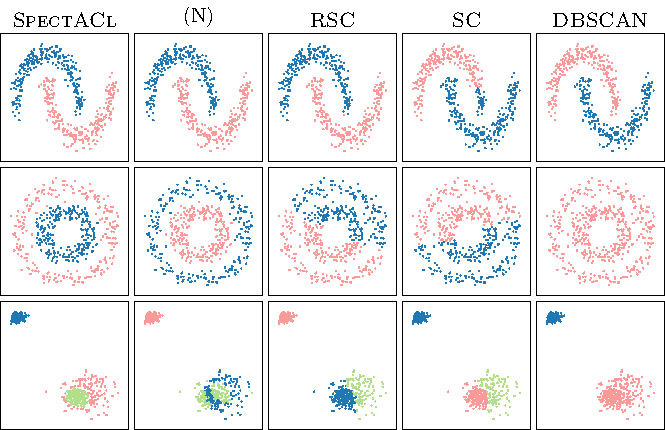
\includegraphics[width=\linewidth]{pics/SASynthScatter.pdf}
%\documentclass[preview=true]{standalone}
\usepackage{amsmath,amssymb,nicefrac,bbm}
\usepackage{pdfathesis}
\usepackage{etex}
\usepackage{xcolor}
\usepackage[a4paper,left=3.5cm,right=2.5cm,bottom=3.5cm,top=3cm]{geometry}
\usepackage[english]{babel}
\usepackage[round]{natbib}
\usepackage{graphicx,tikz}
\usetikzlibrary{matrix,decorations.pathreplacing, calc, positioning}
\usepackage{relsize} % mathlarger
%\usepackage{hyperref,url}
\usepackage{url}
\usepackage{silence}
\WarningFilter{latex}{Overwriting file}

\usepackage[colorinlistoftodos]{todonotes}
\reversemarginpar
\setlength{\marginparwidth}{3.1cm}
% Theorem-Umgebungen
%\usepackage[amsmath,thmmarks]{ntheorem}
\usepackage{amsthm}
\usepackage{thmtools, thm-restate}
\usepackage{algorithm,algpseudocode}
\algnewcommand{\IIf}[1]{\State\algorithmicif\ #1\ \algorithmicthen}
\algnewcommand{\EndIIf}{\unskip\ \algorithmicend\ \algorithmicif}

\usepackage{enumerate}
\usepackage{booktabs,multirow,adjustbox}
\usepackage[font=small,labelfont=bf]{caption}
\usepackage{subfigure}
\usepackage{pgfplots,filecontents,pgfplotstable}
\usepgfplotslibrary{groupplots}
\pgfplotsset{compat=1.14}
\pgfplotsset{
cohStyle/.style={ctrust,mark options ={ctrust},mark repeat={4}, ultra thick, error bars/.cd,y dir = both, y explicit},
densStyle/.style={cdens,dashed,mark options ={cdens},mark repeat={4}, ultra thick, error bars/.cd,y dir = both, y explicit},
primpStyle/.style={cPrimp,dashed,mark=triangle*,mark options ={cPrimp},mark repeat={3}, ultra thick, error bars/.cd,y dir = both, y explicit},
panStyle/.style={cPan,dashed,mark options ={cPan},mark repeat={3}, ultra thick, error bars/.cd,y dir = both, y explicit},
specStyle/.style={cSpec,mark options ={cSpec},mark repeat={4}, thick, error bars/.cd,y dir = both, y explicit},
specLStyle/.style={cSpecL,mark options ={cSpecL},mark repeat={4}, thick, error bars/.cd,y dir = both, y explicit},
RSCStyle/.style={cRSC,dashed,mark=triangle*,mark options ={cRSC},mark repeat={3}, thick, error bars/.cd,y dir = both, y explicit},
SCStyle/.style={cSC,dashed,mark options ={cSC},mark repeat={3}, thick, error bars/.cd,y dir = both, y explicit},
DBSCANStyle/.style={cDBSCAN,dashed,mark options ={cDBSCAN},mark repeat={3}, thick, error bars/.cd,y dir = both, y explicit},
clusterScatterStyle/.style={scatter/classes={1={cSpecL}, 2={cRSC}, 0={cDBSCAN}, -1={white}},
    scatter, only marks, mark size =0.3, scatter src=explicit symbolic},
nonnegScatterStyle/.style={scatter, only marks, fill=cSpec, scatter src=explicit,
     	visualization depends on ={\thisrow{z} \as \perpointmarksize},
     scatter/@pre marker code/.append style={/tikz/mark size=1.5*\perpointmarksize}},
pandaStyle/.style={cPanda,dashed,mark options ={cPanda},mark repeat={3}, ultra thick, error bars/.cd,y dir = both, y explicit},
punkStyle/.style={cPunk,mark options ={cPunk},mark repeat={3}, thick, error bars/.cd,y dir = both, y explicit},
dbssl1Style/.style={cDBSSL1,dashed,mark options ={cDBSSL1},mark=triangle,mark repeat={3}, thick, error bars/.cd,y dir = both, y explicit},
dbssl2Style/.style={cDBSSL2,dashed,mark options ={cDBSSL2},mark=diamond,mark repeat={3}, thick, error bars/.cd,y dir = both, y explicit},
mdlDbsslStyle/.style={cMDLDBSSL,dashed,mark=star,mark options ={cMDLDBSSL},mark repeat={3}, thick, error bars/.cd,y dir = both, y explicit},
% color change for embedding visualization (fuzzy clusters) 
colormap={test}{[2pt]
    rgb255=(166,206,227);
    rgb255=(166,206,227);
},
}

\Title{ A Mathematical Theory of Making Hard Decisions:
Model Selection and Robustness of Matrix Factorization with Binary
Constraints}

%List of Symbols
\usepackage{nomencl}
\makenomenclature


%\usepackage{color}
\definecolor{col1}{RGB}{166,206,227}
\definecolor{col2}{RGB}{31,120,180}
\definecolor{col3}{RGB}{178,223,138}
\definecolor{col4}{RGB}{51,160,44}
\definecolor{col5}{RGB}{251,154,153}
\definecolor{col6}{RGB}{227,26,28}

\definecolor{cdens}{named}{col1}
\definecolor{ctrust}{named}{col2}
\definecolor{cPrimp}{named}{col3}
\definecolor{cPan}{named}{col4}
\definecolor{cPanda}{named}{col5}
\definecolor{cNassau}{named}{col6}
\definecolor{cMdl4bmf}{named}{col1}


%
\definecolor{cSpec}{named}{col1}
\definecolor{cSpecL}{named}{col2}
\definecolor{cRSC}{named}{col3}
\definecolor{cSC}{named}{col4}
\definecolor{cDBSCAN}{named}{col5}

%
\definecolor{cPunk}{named}{col1}
\definecolor{cDBSSL1}{named}{col2}
\definecolor{cDBSSL2}{named}{col4}
\definecolor{cMDLDBSSL}{named}{col5}
% Theorem-Optionen %
%\theoremseparator{.}
%\newenvironment{proof}{\par\noindent{\textit{ Proof}\ }}{\hfill\qed\\[2mm]}
\theoremstyle{plain}
%\theoremheaderfont{\moon}
%\newcommand{\BlackBox}{\rule{1.5ex}{1.5ex}}  % end of proof
%
\newtheorem{theorem}{Theorem}[chapter]
\newtheorem{corollary}[theorem]{Corollary}
\newtheorem{observation}[theorem]{Observation}
\newtheorem{lemma}[theorem]{Lemma}
%\theorembodyfont{\upshape}
\theoremstyle{definition}
\newtheorem{definition}[theorem]{Definition}
\newtheorem{algSpec}{Algorithm Specification}
\newtheorem*{remark}{Remark}
\newtheorem*{example}{Example}
\newtheorem*{problem}{Problem}

%Operators/Commands
\DeclareMathOperator*{\argmin}{arg\,min}
\DeclareMathOperator*{\argmax}{arg\,max}
\DeclareMathOperator*{\freq}{freq}
\DeclareMathOperator*{\cov}{cov}
\DeclareMathOperator*{\anc}{anc}
\DeclareMathOperator*{\supp}{supp}
\DeclareMathOperator*{\minsup}{minsup}
\DeclareMathOperator*{\tr}{tr}
\DeclareMathOperator*{\bigO}{\mathcal{O}}
\DeclareMathOperator{\diag}{diag}
\DeclareMathOperator{\prox}{prox}
\DeclareMathOperator{\pre}{pre}
\DeclareMathOperator{\rec}{rec}
\newcommand{\Ya}{Y_{\mathcal{J}_a\cdot}}
\newcommand{\Va}{{V_a}}
\newcommand{\Da}{D_{\mathcal{J}_a\cdot}}
\newcommand{\KL}{Kurdyka-{\L}ojasiewicz }
\newcommand{\LXU}{\mathcal{L}}
\newcommand{\F}{\mathcal{F}}
\newcommand{\N}{\mathbb{N}}
\newcommand{\R}{\mathbb{R}}
\newcommand{\estU}{\widetilde{U}_{\widehat{CT}}}
\newcommand{\estu}{\tilde{u}_{\widehat{CT}}}
\newcommand{\estCT}{\widehat{CT}}
\newcommand{\node}{\mathfrak{n}}
\newcommand{\leaf}{\mathfrak{t}}
\newcommand{\krimp}{\textsc{Krimp} }
\newcommand{\shrimp}{\textsc{SHrimp} }
\newcommand{\slim}{\textsc{Slim} }

\makeatletter

\pgfplotstableset{
    zero color/.initial=white,
    zero color/.get=\zerocol,
    zero color/.store in=\zerocol,
    one color/.initial=red,
    one color/.get=\onecol,
    one color/.store in=\onecol,
    color cells/.style={
        every head row/.style={output empty row},
        string type,
        postproc cell content/.code={%
           \pgfkeysalso{@cell content=\rule{0cm}{2.4ex}\cellcolor{\zerocol}
           \pgfmathtruncatemacro\number{int(##1)}
           \ifnum\number>100\cellcolor{\onecol!50!black}
           \else \ifnum\number>0\cellcolor{\onecol!##1}\fi\fi}%
        },
        columns/x/.style={
            column name={},
            postproc cell content/.code={}
        }
    }
}
\makeatother

\makeatletter
\newcommand\footnoteref[1]{\protected@xdef\@thefnmark{\ref{#1}}\@footnotemark}
\makeatother

\makeatletter
%\renewcommand{\@chapapp}{}% Not necessary...
\newenvironment{chapquote}[2][2em]
  {\setlength{\@tempdima}{#1}%
   \def\chapquote@author{#2}%
   \parshape 1 \@tempdima \dimexpr\textwidth-2\@tempdima\relax%
   \itshape}
  {\par\normalfont\hfill--\ \chapquote@author\hspace*{\@tempdima}\par\bigskip}
\makeatother

%Thicker bar
\makeatletter
\newcommand{\thickbar}{\mathpalette\@thickbar}
\newcommand{\@thickbar}[2]{{#1\mkern1.5mu\vbox{
  \sbox\z@{$#1\mkern-1.5mu#2\mkern-1.5mu$}%
  \sbox\tw@{$#1\overline{#2}$}%
  \dimen@=\dimexpr\ht\tw@-\ht\z@-.8\p@\relax
  \hrule\@height.8\p@ % adjust for the desired rule thickness
  \vskip\dimen@
  \box\z@}\mkern1.5mu}
}
\makeatother

%----------box---------------
\usepackage[many]{tcolorbox}
\tcbset{
  myhlight/.style={
    colback=cyan!10,
    arc=0pt,
    outer arc=0pt,
    boxrule=0pt,
    top=2pt,
    bottom=2pt,
    left=2pt,
    right=2pt,
  },
  highlight math style={myhlight},
  mybx/.style={
    colback=white,
    arc=0pt,
    outer arc=0pt,
    boxrule=1pt,
    top=2pt,
    bottom=2pt,
    left=2pt,
    right=2pt,
  }
}

\newtcolorbox{mybox}{
	boxsep=1pt,
  	breakable,
  	mybx
}


% Zeilenabstand einstellen %
\renewcommand{\baselinestretch}{1}
% Floating-Umgebungen anpassen %
\renewcommand{\topfraction}{1.0}
\renewcommand{\bottomfraction}{1.0}
\renewcommand{\floatpagefraction}{1.0}
\renewcommand{\dblfloatpagefraction}{1.0}

% Leere Seite ohne Seitennummer, naechste Seite rechts
\newcommand{\blankpage}{
 \clearpage{\pagestyle{empty}\cleardoublepage}
}

% Keine einzelnen Zeilen beim Anfang eines Abschnitts (Schusterjungen)
\clubpenalty = 10000
% Keine einzelnen Zeilen am Ende eines Abschnitts (Hurenkinder)
\widowpenalty = 10000 \displaywidowpenalty = 10000
% EOF
%
\begin{document}
%
\begin{filecontents}{nmSpectACl_eps.dat}
x y z
1.70069743062 2.42758078324 1
0.285683163483 0.820224134154 1
1.96043338205 1.11652004199 1
2.54379828594 0.801796530514 0
1.02584883691 2.57355440485 1
1.93164886191 1.28604223276 1
1.83409801343 1.05168575212 1
1.50665839702 0.598828682981 0
1.21456049586 1.91816830754 0
0.548489010379 2.4266670795 1
2.43718937566 0.259585631612 0
1.08815940258 1.49111722436 0
1.03453098116 1.5879904518 0
0.109412219779 1.28023561758 1
1.9865620235 1.22135031104 1
1.22512830724 1.0225006133 0
2.86565022133 1.80367677252 0
2.89706812992 1.53195814064 0
0.8209715405 1.72041831352 0
0.617806017378 2.40727584262 1
2.28442347034 0.430331423047 0
1.28180236997 1.03358907376 0
0.887937054635 2.68053646933 1
0.891570602061 2.32922789032 1
2.65618201755 0.894877000626 0
0.498394232883 2.45236217747 1
1.35694280656 2.46718908062 1
1.11489573331 1.85699692515 0
2.9080680088 1.73914577833 0
0.785679177354 2.44215259264 1
0.196823873853 1.89256063131 1
1.17823524744 1.75551785493 0
1.23992030311 2.66315904413 1
2.00540849232 0.499253921452 0
0.848956944163 2.45868527982 1
0.0925078051445 1.29305455349 1
0.247138803261 1.95645113223 1
2.83766305835 1.76420767232 0
1.12807120931 1.38527205119 0
1.94201627226 1.40478582163 1
1.25729757329 1.8930319065 0
1.89326303725 1.91932512895 1
1.72383858092 2.21738324713 1
0.45709546568 2.4199525741 1
1.35307081946 2.21860026432 1
1.00887362506 1.94033464961 0
2.34181723671 0.686515872943 0
1.11475444609 0.954182702693 0
0.420448354856 2.32241979328 1
1.59149868632 2.16078316015 1
0.329310350731 1.82923651818 1
0.629423152641 2.36690609361 1
0.307287028638 1.63670049795 1
2.59724264213 0.569519846613 0
0.527392241622 2.54113453641 1
1.91786921713 0.481595165812 0
1.95156790129 2.12611147089 1
1.41194255779 2.66793976628 1
0.0694222959687 1.82183402009 1
1.61367440743 0.544603242775 0
1.84906416078 1.43524726088 1
2.56840153548 0.978613872479 0
2.68782194498 1.60369331079 0
1.6967066369 2.05018333769 1
0.287779916276 1.35181404437 1
2.10581182305 0.58600544124 0
2.76589189346 1.31793021207 0
0.903330891708 2.71981111471 1
1.78910702143 1.78431684787 1
2.85201486168 1.75683049978 0
2.61444426339 1.1421123448 0
1.76686652891 0.412643118932 0
2.38343223857 0.614019382719 0
0.351982420161 1.82124180438 1
1.20104638372 1.08550087193 0
1.71310358783 2.10563588448 1
1.20574320869 1.14241676927 0
1.85476278831 1.68570217527 1
0.866928473775 2.71912423537 1
1.24150157057 1.87008926301 0
1.28290021851 2.54224942198 1
2.20513157208 0.332694252519 0
0.7649274204 2.49776682771 1
1.92833706433 1.74896192577 1
1.12650480957 1.0348913114 0
0.42035554481 2.29433128095 1
1.8227778128 1.73009804176 1
1.40440087482 0.800372448393 0
0.350170029196 1.83113326458 1
2.67833915261 0.955760684365 0
1.45206309833 2.3376423972 1
1.99881809264 0.647288007188 0
1.73930300342 2.27513141315 1
0.997530664835 2.48601880132 1
2.52748209417 0.964779854994 0
0.18616961175 1.41798846544 1
1.27951506157 0.579681303838 0
1.24451979199 1.01467765734 0
1.528155426 0.429507299506 0
1.86116862662 0.0 0
0.229448043123 1.39451828581 1
2.43840791486 0.811277652094 0
1.08024324217 1.45606914327 0
1.69141952321 1.87996999864 1
0.523342152062 2.27879186696 1
2.53685907702 0.842989476903 0
0.781622595306 2.37059793943 1
2.37151355968 0.752368295204 0
1.81585388656 0.405096626174 0
0.526353426641 2.28139242049 1
2.7760661566 0.95760548246 0
0.923603269543 2.64416122336 1
1.94640723913 1.91848140563 1
1.56063634725 2.50248629435 1
1.0176090148 2.72395908515 1
2.31363407826 0.5281707426 0
1.73803401456 1.88934225142 1
0.26732734312 1.01993624365 1
1.92620482073 1.36669614426 1
2.83528847849 2.08551281403 0
1.2560191234 0.92058406981 0
2.38592708362 0.628151589247 0
1.63132977838 0.709002849989 0
1.05904065429 1.51493849809 0
0.139685121871 1.80990844772 1
1.27499215905 1.06475398303 0
1.14937169414 1.42166121091 0
2.33215946967 0.30036289709 0
1.67510627109 0.411176705111 0
1.18231701939 2.50556350357 1
1.77038669418 1.7965018847 1
2.41711258717 1.06425648687 0
1.5466743199 2.19799847606 1
2.81159915284 0.84108084496 0
2.09568775447 0.361760404015 0
1.62856213766 2.40924498166 1
2.39833092966 0.493171096231 0
1.51465143737 2.47271499647 1
1.13635348992 0.947616890809 0
1.04349043595 1.39023226786 0
0.603031169212 2.58849736575 1
1.9387998979 1.22409851527 1
0.128778294394 1.31392528176 1
1.1003283767 1.2661573588 0
0.743838019158 2.52252993124 1
0.61621116068 2.65631385961 1
0.886728816447 2.57220887 1
1.93703048927 0.497335966775 0
1.34132891502 0.890984584948 0
0.536517048738 2.03140735086 1
0.426818260547 2.19895923382 1
0.382225086449 2.24212488028 1
0.90075749994 2.84889611659 1
1.71053267234 0.139893439754 0
1.29639938455 2.59086974776 1
1.94208010739 0.301786108633 0
1.83766716651 1.89862578133 1
0.217910019358 1.18284981176 1
2.87431916031 1.13362681065 0
2.49128297904 0.808660342234 0
0.887367512053 1.77483826418 0
2.41849255062 0.5324350021 0
1.52025137653 2.40917722219 1
2.81144168216 1.32711652029 0
1.04959124228 1.45154913004 0
2.76797402357 1.57360077806 0
1.82169413997 1.6359444949 1
0.463673012107 2.13666946634 1
1.76717691103 0.185518641762 0
1.79700009392 0.415992627791 0
1.07371926343 1.25433471066 0
0.35340797154 2.20777111939 1
0.910470573245 2.57545855259 1
1.00666113925 1.41487472942 0
0.263242311008 2.11420843779 1
1.83750587555 0.960921001284 1
0.598118607947 2.17126465619 1
0.989607517794 2.72016213659 1
0.339991852275 1.6367039174 1
2.81553150588 1.25227670267 0
1.1688157054 1.61925018628 0
2.87702213607 1.62065697172 0
1.18784418709 1.07176694342 0
2.69535677668 1.14397649917 0
2.61215137255 0.908888019432 0
2.2703000471 0.739737480907 0
0.310292767944 1.5927524401 1
1.9751498572 1.39478059397 1
1.05585797661 1.86898397783 0
0.491864333665 2.31875950071 1
2.04280176433 0.227220807369 0
1.29239733899 2.77729312657 1
1.76399564245 0.389462528366 0
1.10987143975 2.45825835483 1
0.888789567782 2.65387087803 1
2.45980643174 0.992909318285 0
1.08897922761 1.42887358233 0
0.759086710455 2.40740216785 1
2.85579700003 1.62503776295 0
1.49047821489 0.578651837622 0
2.14306688802 0.410252695811 0
2.80690341525 1.04739831031 0
1.08084426927 2.37142988192 1
1.24156411616 1.55517287562 0
1.46082893365 0.841033454439 0
1.13147127699 2.53816467841 1
2.47534170514 0.691577879525 0
0.515186721621 2.37712522384 1
0.738658590011 2.23721041569 1
0.152209727518 1.84671174913 1
2.60849673113 0.841526842613 0
1.04231829692 2.71045161422 1
0.964376417508 1.74174356827 0
0.342359603748 2.31301969708 1
0.312328480287 2.0697583552 1
2.45657728683 0.742808305141 0
1.96519472004 1.95521093343 1
0.976026718348 1.65145435908 0
1.70038574297 0.690680548668 0
1.37321471501 0.593617808351 0
1.34431592493 2.38004670142 1
1.20432098055 1.41547092441 0
1.0929063259 1.64510555084 0
1.14149626236 1.27251025565 0
2.38350457204 0.579440777335 0
1.29738017256 2.28865081481 1
1.19200628952 1.85807567095 0
2.29057019712 0.494581835568 0
1.80036719203 2.25739553896 1
1.7374178378 0.17861431239 0
0.681070242517 2.21529849059 1
1.88653779019 1.71753481275 1
1.66130686 0.453575429025 0
1.05708950661 1.30651646662 0
1.7262189757 2.0892030765 1
1.8743608435 1.34263072606 1
1.48620524338 0.715922906298 0
2.00459538411 0.635140423792 0
0.318587109448 1.92679150556 1
1.37843639956 0.707088283144 0
2.60563623353 0.84239504921 0
2.51013047406 1.15186988552 0
1.09765232658 2.56485848597 1
2.65051441579 0.706858112677 0
0.352710453599 1.60528124984 1
1.367034677 2.342617793 1
2.6778340428 1.27583043688 0
2.77041498717 1.62149290572 0
0.433413700012 2.28661466553 1
2.48279234082 0.838028620621 0
0.664103039947 2.61890924636 1
0.485901366946 2.02729851019 1
1.85342076722 0.311040878791 0
2.24141958751 0.69211889508 0
1.05284501061 0.815302813624 0
1.79533297587 1.72925735288 1
1.59592524946 2.291103752 1
1.12311889981 2.73494294316 1
0.239642607379 1.4708710286 1
2.38074908517 0.178741070048 0
1.95942048639 0.485758418579 0
0.801008762883 2.35832224956 1
1.74336065112 2.52814028379 1
2.00425063315 1.44973882129 1
2.99874263731 1.61490975065 0
1.77010542011 2.37104764753 1
1.512850527 2.28856440723 1
2.45235640311 0.561489373791 0
1.295122251 0.789267498929 0
1.51455075898 0.528202376017 0
0.304527789681 1.21175257382 1
1.21559659311 0.781644945741 0
2.13154242053 0.328030655553 0
1.02901463251 1.60574602789 0
1.04967754137 2.46974317694 1
0.383986869727 1.946959298 1
0.674587230211 2.31409008533 1
2.94816733924 1.82970946363 0
1.46163323762 0.792251773345 0
0.660363196201 2.44792160823 1
2.03001716038 0.213480207542 0
1.36368239515 0.799287249057 0
0.100287359104 1.22065856204 1
2.01060150251 0.464874464476 0
2.02983745816 0.305243543361 0
1.2251556746 1.52746937796 0
2.69691681725 1.71441309537 0
2.85609415251 1.41314756677 0
1.01887468848 2.53297875059 1
1.72087173411 1.97290485697 1
0.0540782987346 1.66034457313 1
1.50772484392 0.172194489983 0
1.24910710679 0.732983283934 0
1.21965279462 1.48366422323 0
1.62105492439 2.04589281976 1
2.87108229353 1.48089493044 0
2.86550061675 1.67997945483 0
1.09627892364 1.65438075877 0
0.338132847221 1.79813179713 1
0.436675834273 2.29829461324 1
1.35612302258 0.617635762047 0
2.71578839431 1.11238360205 0
1.84067753076 2.35076159932 1
1.90883244213 1.40654781879 1
0.448930144962 2.42194163441 1
2.27088828505 0.720328288284 0
1.99427584167 0.292469923157 0
2.05179138307 0.075191975576 0
2.75775762337 1.41657699478 0
0.12405803592 1.67542521447 1
2.43818544068 0.725956693576 0
0.312635410658 1.46319738786 1
0.191240314346 1.65611706549 1
2.75529018146 1.51664712917 0
2.87438941247 1.42513159143 0
1.6124710734 0.108162333984 0
2.07748229347 1.37016700533 1
1.34233953375 0.80510418713 0
0.402666931541 1.97206849653 1
1.59991006122 0.430928345538 0
1.76450324322 1.9417972377 1
0.68142574163 2.3657937995 1
0.164887719809 0.933208295559 1
0.917202040984 2.45367836822 1
0.162413262346 1.79806447542 1
1.69954497521 0.474876958658 0
0.885974873525 2.80037127387 1
1.51432134071 2.26982073221 1
1.34621921819 0.906396320943 0
0.691126264848 2.70915758443 1
1.87293313667 1.78727508456 1
2.28649531765 0.726889577091 0
1.07263048888 2.68627388773 1
1.80060022058 0.599304932113 0
1.26924503947 2.54861366445 1
1.05684697644 1.91308852172 0
1.34125453355 0.95711539541 0
2.8125803328 1.52002754851 0
1.21682707227 0.904424035905 0
1.31929933512 2.79201230232 1
0.637404952623 2.32382669843 1
2.17137726399 0.282323068269 0
1.62762538368 2.26290014007 1
0.540666367159 2.33600275939 1
1.88293690233 1.28480350699 1
2.77912006373 1.9726418669 0
0.887955978785 2.55238946452 1
1.85499981106 2.17561046177 1
2.77275743931 1.26672052764 0
1.88408081212 1.55654855145 1
2.20422656878 0.194151609861 0
1.37215670775 0.64239160578 0
2.74173332893 1.06281332167 0
1.3519692899 2.44789629152 1
0.976624716971 1.76062464088 0
1.04508085459 1.58720561346 0
1.86316148119 0.606405006819 0
1.84838679137 0.364768005124 0
0.3387851597 2.31151471375 1
0.695323634969 2.53219749966 1
1.5016800772 2.28286263615 1
1.72601415658 0.425192245283 0
2.7956168279 1.41300555516 0
0.575132420922 2.21555668975 1
1.92736865662 1.30428244235 1
2.86941042658 1.12652831483 0
0.505972295319 2.11848657916 1
2.88083111935 1.79685857086 0
1.54968608895 2.50447888087 1
2.31278971533 0.259675335988 0
2.73879578515 1.18969715242 0
2.41045930274 0.901294611205 0
0.174601175717 1.25065471515 1
2.32186139204 0.515582850319 0
0.20554231582 1.35225498011 1
2.73059185626 1.20383151563 0
1.3865034904 2.53822490098 1
1.12900900657 2.75114078017 1
0.115069738958 1.04596772082 1
1.335120272 2.64619551797 1
0.831696677651 2.37593629365 1
0.292063587839 1.88454278761 1
1.40477301971 2.48630866567 1
0.227853652523 1.72614884781 1
1.39895080992 2.73195382504 1
2.74706816704 1.76622164219 0
1.65483832512 2.04749839106 1
1.9617597714 0.486798653141 0
1.64888491758 2.17115329123 1
1.60586723589 0.501084875631 0
0.284675287626 1.34679532238 1
1.7675237627 2.24242168385 1
1.26193391783 2.60789114088 1
1.85894079362 1.62496524757 1
1.23674367127 0.982304806675 0
1.97582138089 0.509380358308 0
1.05600781745 2.677392365 1
0.184110621272 2.05447883901 1
0.547385160286 2.55233290655 1
2.57887948172 0.828032733195 0
0.207424483914 1.40821380306 1
1.4369592134 2.72855234245 1
1.62259449811 1.74010086385 1
2.672451501 1.6291678069 0
1.81325243451 0.253878981216 0
1.6389068495 2.55396535903 1
1.78009058629 1.82382255609 1
1.82405310361 2.18872776439 1
0.297924979561 2.15608602252 1
0.734938555418 2.43601614007 1
2.76539867309 0.876829399765 0
0.299689834261 2.26240499707 1
0.657100676443 2.54932984854 1
1.97531757625 0.418517119017 0
1.70335971574 2.01957604536 1
2.01136443846 1.56650446432 1
1.9889246753 1.33708935655 1
0.520697457737 2.19392438309 1
0.201610918869 1.11114702728 1
1.18460310214 2.64018309532 1
1.67953679203 2.09096852593 1
2.52903300028 0.668689176375 0
1.82992609123 0.41148308689 0
1.8782077118 1.15964218423 1
2.77296228387 1.32572928549 0
1.82869717065 0.425653875063 0
0.894053475273 2.44439263156 1
1.07621362954 1.70969278243 0
1.45644007418 2.18215955599 1
1.22063523709 1.744321168 0
1.07967091239 1.06274577676 0
1.1900696085 1.26923933736 0
1.04550909582 1.95159439522 0
1.36599613108 0.996983555907 0
1.48939507438 2.55035208922 1
1.39352940488 0.963024804974 0
1.79847337348 1.76745116277 1
2.79775175948 0.989798501929 0
1.85447215813 0.591984136577 0
1.97133310695 1.23755879013 1
1.33548899995 0.903694832059 0
1.24331015073 2.6153250888 1
1.18889713657 2.78378504495 1
0.959819003516 1.85803345242 0
1.48688739481 0.518828000145 0
2.17038326017 0.538678939108 0
2.00401389267 1.2148267132 1
1.80471537631 1.56843402421 1
2.41227229935 0.418729119508 0
1.54810143205 0.592880123322 0
2.70786075559 1.37847478472 0
1.95754047284 1.18045687789 1
0.376516805236 1.88573157828 1
1.55659448472 1.89138211448 1
1.6713666353 0.452084078249 0
2.01552714856 0.493164592727 0
2.92882892778 1.71535055117 0
2.30685921255 0.69876892802 0
0.910811583335 2.47994266873 1
1.20418470115 2.33843955069 1
2.39790481126 0.794684627456 0
2.46701618738 0.581809838238 0
0.251366988518 1.8780274577 1
0.499412691579 2.38088700981 1
2.56205261531 0.65140655269 0
0.421518010626 2.06060390571 1
1.17009887948 1.5134267149 0
2.81288537691 1.68955621988 0
1.85801783879 0.555828770401 0
1.62002253434 2.06714531107 1
0.587232551254 2.47998567591 1
0.929550119504 2.62696249914 1
0.285941297863 1.76825739547 1
0.259015697972 1.26276981669 1
1.90778512029 1.51870006004 1
1.78857330267 0.328932520462 0
1.62111786442 2.21583017128 1
1.55851506264 2.39564830468 1
2.8184718636 1.49831763883 0
1.44366997728 0.811031572419 0
0.670803912622 2.52569944579 1
1.99900347199 1.27336970112 1
1.03545744455 2.67615661925 1
1.94020677429 0.417071861833 0
1.7209951759 0.415479497045 0
2.44397592822 0.627725787503 0
1.38008876818 0.718105733857 0
2.53036245288 0.380380389259 0
1.95319494442 0.992058285038 1
0.983756955407 1.32684250689 0
0.6881145508 2.71837116248 1
1.88019132883 1.60123260018 1
1.29417582527 1.2231395338 0
1.29745287353 2.79297372882 1
0.333622187036 2.26301752448 1
0.32392659893 1.70725807039 1
1.27163496314 2.5038370693 1
0.419549967659 2.16152124321 1
0.70356632396 2.43698318681 1
2.24311863984 0.0606826745953 0
\end{filecontents}
\begin{filecontents}{nmSpectACl_knn_n.dat}
x y z
1.70069743062 2.42758078324 1
0.285683163483 0.820224134154 1
1.96043338205 1.11652004199 1
2.54379828594 0.801796530514 0
1.02584883691 2.57355440485 1
1.93164886191 1.28604223276 1
1.83409801343 1.05168575212 1
1.50665839702 0.598828682981 0
1.21456049586 1.91816830754 0
0.548489010379 2.4266670795 1
2.43718937566 0.259585631612 0
1.08815940258 1.49111722436 0
1.03453098116 1.5879904518 0
0.109412219779 1.28023561758 1
1.9865620235 1.22135031104 1
1.22512830724 1.0225006133 0
2.86565022133 1.80367677252 0
2.89706812992 1.53195814064 0
0.8209715405 1.72041831352 0
0.617806017378 2.40727584262 1
2.28442347034 0.430331423047 0
1.28180236997 1.03358907376 0
0.887937054635 2.68053646933 1
0.891570602061 2.32922789032 1
2.65618201755 0.894877000626 0
0.498394232883 2.45236217747 1
1.35694280656 2.46718908062 1
1.11489573331 1.85699692515 0
2.9080680088 1.73914577833 0
0.785679177354 2.44215259264 1
0.196823873853 1.89256063131 1
1.17823524744 1.75551785493 0
1.23992030311 2.66315904413 1
2.00540849232 0.499253921452 0
0.848956944163 2.45868527982 1
0.0925078051445 1.29305455349 1
0.247138803261 1.95645113223 1
2.83766305835 1.76420767232 0
1.12807120931 1.38527205119 0
1.94201627226 1.40478582163 1
1.25729757329 1.8930319065 0
1.89326303725 1.91932512895 1
1.72383858092 2.21738324713 1
0.45709546568 2.4199525741 1
1.35307081946 2.21860026432 1
1.00887362506 1.94033464961 0
2.34181723671 0.686515872943 0
1.11475444609 0.954182702693 0
0.420448354856 2.32241979328 1
1.59149868632 2.16078316015 1
0.329310350731 1.82923651818 1
0.629423152641 2.36690609361 1
0.307287028638 1.63670049795 1
2.59724264213 0.569519846613 0
0.527392241622 2.54113453641 1
1.91786921713 0.481595165812 0
1.95156790129 2.12611147089 1
1.41194255779 2.66793976628 1
0.0694222959687 1.82183402009 1
1.61367440743 0.544603242775 0
1.84906416078 1.43524726088 1
2.56840153548 0.978613872479 0
2.68782194498 1.60369331079 0
1.6967066369 2.05018333769 1
0.287779916276 1.35181404437 1
2.10581182305 0.58600544124 0
2.76589189346 1.31793021207 0
0.903330891708 2.71981111471 1
1.78910702143 1.78431684787 1
2.85201486168 1.75683049978 0
2.61444426339 1.1421123448 0
1.76686652891 0.412643118932 0
2.38343223857 0.614019382719 0
0.351982420161 1.82124180438 1
1.20104638372 1.08550087193 0
1.71310358783 2.10563588448 1
1.20574320869 1.14241676927 0
1.85476278831 1.68570217527 1
0.866928473775 2.71912423537 1
1.24150157057 1.87008926301 0
1.28290021851 2.54224942198 1
2.20513157208 0.332694252519 0
0.7649274204 2.49776682771 1
1.92833706433 1.74896192577 1
1.12650480957 1.0348913114 0
0.42035554481 2.29433128095 1
1.8227778128 1.73009804176 1
1.40440087482 0.800372448393 0
0.350170029196 1.83113326458 1
2.67833915261 0.955760684365 0
1.45206309833 2.3376423972 1
1.99881809264 0.647288007188 0
1.73930300342 2.27513141315 1
0.997530664835 2.48601880132 1
2.52748209417 0.964779854994 0
0.18616961175 1.41798846544 1
1.27951506157 0.579681303838 0
1.24451979199 1.01467765734 0
1.528155426 0.429507299506 0
1.86116862662 0.0 0
0.229448043123 1.39451828581 1
2.43840791486 0.811277652094 0
1.08024324217 1.45606914327 0
1.69141952321 1.87996999864 1
0.523342152062 2.27879186696 1
2.53685907702 0.842989476903 0
0.781622595306 2.37059793943 1
2.37151355968 0.752368295204 0
1.81585388656 0.405096626174 0
0.526353426641 2.28139242049 1
2.7760661566 0.95760548246 0
0.923603269543 2.64416122336 1
1.94640723913 1.91848140563 1
1.56063634725 2.50248629435 1
1.0176090148 2.72395908515 1
2.31363407826 0.5281707426 0
1.73803401456 1.88934225142 1
0.26732734312 1.01993624365 1
1.92620482073 1.36669614426 1
2.83528847849 2.08551281403 0
1.2560191234 0.92058406981 0
2.38592708362 0.628151589247 0
1.63132977838 0.709002849989 0
1.05904065429 1.51493849809 0
0.139685121871 1.80990844772 1
1.27499215905 1.06475398303 0
1.14937169414 1.42166121091 0
2.33215946967 0.30036289709 0
1.67510627109 0.411176705111 0
1.18231701939 2.50556350357 1
1.77038669418 1.7965018847 1
2.41711258717 1.06425648687 0
1.5466743199 2.19799847606 1
2.81159915284 0.84108084496 0
2.09568775447 0.361760404015 0
1.62856213766 2.40924498166 1
2.39833092966 0.493171096231 0
1.51465143737 2.47271499647 1
1.13635348992 0.947616890809 0
1.04349043595 1.39023226786 0
0.603031169212 2.58849736575 1
1.9387998979 1.22409851527 1
0.128778294394 1.31392528176 1
1.1003283767 1.2661573588 0
0.743838019158 2.52252993124 1
0.61621116068 2.65631385961 1
0.886728816447 2.57220887 1
1.93703048927 0.497335966775 0
1.34132891502 0.890984584948 0
0.536517048738 2.03140735086 1
0.426818260547 2.19895923382 1
0.382225086449 2.24212488028 1
0.90075749994 2.84889611659 1
1.71053267234 0.139893439754 0
1.29639938455 2.59086974776 1
1.94208010739 0.301786108633 0
1.83766716651 1.89862578133 1
0.217910019358 1.18284981176 1
2.87431916031 1.13362681065 0
2.49128297904 0.808660342234 0
0.887367512053 1.77483826418 0
2.41849255062 0.5324350021 0
1.52025137653 2.40917722219 1
2.81144168216 1.32711652029 0
1.04959124228 1.45154913004 0
2.76797402357 1.57360077806 0
1.82169413997 1.6359444949 1
0.463673012107 2.13666946634 1
1.76717691103 0.185518641762 0
1.79700009392 0.415992627791 0
1.07371926343 1.25433471066 0
0.35340797154 2.20777111939 1
0.910470573245 2.57545855259 1
1.00666113925 1.41487472942 0
0.263242311008 2.11420843779 1
1.83750587555 0.960921001284 1
0.598118607947 2.17126465619 1
0.989607517794 2.72016213659 1
0.339991852275 1.6367039174 1
2.81553150588 1.25227670267 0
1.1688157054 1.61925018628 0
2.87702213607 1.62065697172 0
1.18784418709 1.07176694342 0
2.69535677668 1.14397649917 0
2.61215137255 0.908888019432 0
2.2703000471 0.739737480907 0
0.310292767944 1.5927524401 1
1.9751498572 1.39478059397 1
1.05585797661 1.86898397783 0
0.491864333665 2.31875950071 1
2.04280176433 0.227220807369 0
1.29239733899 2.77729312657 1
1.76399564245 0.389462528366 0
1.10987143975 2.45825835483 1
0.888789567782 2.65387087803 1
2.45980643174 0.992909318285 0
1.08897922761 1.42887358233 0
0.759086710455 2.40740216785 1
2.85579700003 1.62503776295 0
1.49047821489 0.578651837622 0
2.14306688802 0.410252695811 0
2.80690341525 1.04739831031 0
1.08084426927 2.37142988192 1
1.24156411616 1.55517287562 0
1.46082893365 0.841033454439 0
1.13147127699 2.53816467841 1
2.47534170514 0.691577879525 0
0.515186721621 2.37712522384 1
0.738658590011 2.23721041569 1
0.152209727518 1.84671174913 1
2.60849673113 0.841526842613 0
1.04231829692 2.71045161422 1
0.964376417508 1.74174356827 0
0.342359603748 2.31301969708 1
0.312328480287 2.0697583552 1
2.45657728683 0.742808305141 0
1.96519472004 1.95521093343 1
0.976026718348 1.65145435908 0
1.70038574297 0.690680548668 0
1.37321471501 0.593617808351 0
1.34431592493 2.38004670142 1
1.20432098055 1.41547092441 0
1.0929063259 1.64510555084 0
1.14149626236 1.27251025565 0
2.38350457204 0.579440777335 0
1.29738017256 2.28865081481 1
1.19200628952 1.85807567095 0
2.29057019712 0.494581835568 0
1.80036719203 2.25739553896 1
1.7374178378 0.17861431239 0
0.681070242517 2.21529849059 1
1.88653779019 1.71753481275 1
1.66130686 0.453575429025 0
1.05708950661 1.30651646662 0
1.7262189757 2.0892030765 1
1.8743608435 1.34263072606 1
1.48620524338 0.715922906298 0
2.00459538411 0.635140423792 0
0.318587109448 1.92679150556 1
1.37843639956 0.707088283144 0
2.60563623353 0.84239504921 0
2.51013047406 1.15186988552 0
1.09765232658 2.56485848597 1
2.65051441579 0.706858112677 0
0.352710453599 1.60528124984 1
1.367034677 2.342617793 1
2.6778340428 1.27583043688 0
2.77041498717 1.62149290572 0
0.433413700012 2.28661466553 1
2.48279234082 0.838028620621 0
0.664103039947 2.61890924636 1
0.485901366946 2.02729851019 1
1.85342076722 0.311040878791 0
2.24141958751 0.69211889508 0
1.05284501061 0.815302813624 0
1.79533297587 1.72925735288 1
1.59592524946 2.291103752 1
1.12311889981 2.73494294316 1
0.239642607379 1.4708710286 1
2.38074908517 0.178741070048 0
1.95942048639 0.485758418579 0
0.801008762883 2.35832224956 1
1.74336065112 2.52814028379 1
2.00425063315 1.44973882129 1
2.99874263731 1.61490975065 0
1.77010542011 2.37104764753 1
1.512850527 2.28856440723 1
2.45235640311 0.561489373791 0
1.295122251 0.789267498929 0
1.51455075898 0.528202376017 0
0.304527789681 1.21175257382 1
1.21559659311 0.781644945741 0
2.13154242053 0.328030655553 0
1.02901463251 1.60574602789 0
1.04967754137 2.46974317694 1
0.383986869727 1.946959298 1
0.674587230211 2.31409008533 1
2.94816733924 1.82970946363 0
1.46163323762 0.792251773345 0
0.660363196201 2.44792160823 1
2.03001716038 0.213480207542 0
1.36368239515 0.799287249057 0
0.100287359104 1.22065856204 1
2.01060150251 0.464874464476 0
2.02983745816 0.305243543361 0
1.2251556746 1.52746937796 0
2.69691681725 1.71441309537 0
2.85609415251 1.41314756677 0
1.01887468848 2.53297875059 1
1.72087173411 1.97290485697 1
0.0540782987346 1.66034457313 1
1.50772484392 0.172194489983 0
1.24910710679 0.732983283934 0
1.21965279462 1.48366422323 0
1.62105492439 2.04589281976 1
2.87108229353 1.48089493044 0
2.86550061675 1.67997945483 0
1.09627892364 1.65438075877 0
0.338132847221 1.79813179713 1
0.436675834273 2.29829461324 1
1.35612302258 0.617635762047 0
2.71578839431 1.11238360205 0
1.84067753076 2.35076159932 1
1.90883244213 1.40654781879 1
0.448930144962 2.42194163441 1
2.27088828505 0.720328288284 0
1.99427584167 0.292469923157 0
2.05179138307 0.075191975576 0
2.75775762337 1.41657699478 0
0.12405803592 1.67542521447 1
2.43818544068 0.725956693576 0
0.312635410658 1.46319738786 1
0.191240314346 1.65611706549 1
2.75529018146 1.51664712917 0
2.87438941247 1.42513159143 0
1.6124710734 0.108162333984 0
2.07748229347 1.37016700533 1
1.34233953375 0.80510418713 0
0.402666931541 1.97206849653 1
1.59991006122 0.430928345538 0
1.76450324322 1.9417972377 1
0.68142574163 2.3657937995 1
0.164887719809 0.933208295559 1
0.917202040984 2.45367836822 1
0.162413262346 1.79806447542 1
1.69954497521 0.474876958658 0
0.885974873525 2.80037127387 1
1.51432134071 2.26982073221 1
1.34621921819 0.906396320943 0
0.691126264848 2.70915758443 1
1.87293313667 1.78727508456 1
2.28649531765 0.726889577091 0
1.07263048888 2.68627388773 1
1.80060022058 0.599304932113 0
1.26924503947 2.54861366445 1
1.05684697644 1.91308852172 0
1.34125453355 0.95711539541 0
2.8125803328 1.52002754851 0
1.21682707227 0.904424035905 0
1.31929933512 2.79201230232 1
0.637404952623 2.32382669843 1
2.17137726399 0.282323068269 0
1.62762538368 2.26290014007 1
0.540666367159 2.33600275939 1
1.88293690233 1.28480350699 1
2.77912006373 1.9726418669 0
0.887955978785 2.55238946452 1
1.85499981106 2.17561046177 1
2.77275743931 1.26672052764 0
1.88408081212 1.55654855145 1
2.20422656878 0.194151609861 0
1.37215670775 0.64239160578 0
2.74173332893 1.06281332167 0
1.3519692899 2.44789629152 1
0.976624716971 1.76062464088 0
1.04508085459 1.58720561346 0
1.86316148119 0.606405006819 0
1.84838679137 0.364768005124 0
0.3387851597 2.31151471375 1
0.695323634969 2.53219749966 1
1.5016800772 2.28286263615 1
1.72601415658 0.425192245283 0
2.7956168279 1.41300555516 0
0.575132420922 2.21555668975 1
1.92736865662 1.30428244235 1
2.86941042658 1.12652831483 0
0.505972295319 2.11848657916 1
2.88083111935 1.79685857086 0
1.54968608895 2.50447888087 1
2.31278971533 0.259675335988 0
2.73879578515 1.18969715242 0
2.41045930274 0.901294611205 0
0.174601175717 1.25065471515 1
2.32186139204 0.515582850319 0
0.20554231582 1.35225498011 1
2.73059185626 1.20383151563 0
1.3865034904 2.53822490098 1
1.12900900657 2.75114078017 1
0.115069738958 1.04596772082 1
1.335120272 2.64619551797 1
0.831696677651 2.37593629365 1
0.292063587839 1.88454278761 1
1.40477301971 2.48630866567 1
0.227853652523 1.72614884781 1
1.39895080992 2.73195382504 1
2.74706816704 1.76622164219 0
1.65483832512 2.04749839106 1
1.9617597714 0.486798653141 0
1.64888491758 2.17115329123 1
1.60586723589 0.501084875631 0
0.284675287626 1.34679532238 1
1.7675237627 2.24242168385 1
1.26193391783 2.60789114088 1
1.85894079362 1.62496524757 1
1.23674367127 0.982304806675 0
1.97582138089 0.509380358308 0
1.05600781745 2.677392365 1
0.184110621272 2.05447883901 1
0.547385160286 2.55233290655 1
2.57887948172 0.828032733195 0
0.207424483914 1.40821380306 1
1.4369592134 2.72855234245 1
1.62259449811 1.74010086385 1
2.672451501 1.6291678069 0
1.81325243451 0.253878981216 0
1.6389068495 2.55396535903 1
1.78009058629 1.82382255609 1
1.82405310361 2.18872776439 1
0.297924979561 2.15608602252 1
0.734938555418 2.43601614007 1
2.76539867309 0.876829399765 0
0.299689834261 2.26240499707 1
0.657100676443 2.54932984854 1
1.97531757625 0.418517119017 0
1.70335971574 2.01957604536 1
2.01136443846 1.56650446432 1
1.9889246753 1.33708935655 1
0.520697457737 2.19392438309 1
0.201610918869 1.11114702728 1
1.18460310214 2.64018309532 1
1.67953679203 2.09096852593 1
2.52903300028 0.668689176375 0
1.82992609123 0.41148308689 0
1.8782077118 1.15964218423 1
2.77296228387 1.32572928549 0
1.82869717065 0.425653875063 0
0.894053475273 2.44439263156 1
1.07621362954 1.70969278243 0
1.45644007418 2.18215955599 1
1.22063523709 1.744321168 0
1.07967091239 1.06274577676 0
1.1900696085 1.26923933736 0
1.04550909582 1.95159439522 0
1.36599613108 0.996983555907 0
1.48939507438 2.55035208922 1
1.39352940488 0.963024804974 0
1.79847337348 1.76745116277 1
2.79775175948 0.989798501929 0
1.85447215813 0.591984136577 0
1.97133310695 1.23755879013 1
1.33548899995 0.903694832059 0
1.24331015073 2.6153250888 1
1.18889713657 2.78378504495 1
0.959819003516 1.85803345242 0
1.48688739481 0.518828000145 0
2.17038326017 0.538678939108 0
2.00401389267 1.2148267132 1
1.80471537631 1.56843402421 1
2.41227229935 0.418729119508 0
1.54810143205 0.592880123322 0
2.70786075559 1.37847478472 0
1.95754047284 1.18045687789 1
0.376516805236 1.88573157828 1
1.55659448472 1.89138211448 1
1.6713666353 0.452084078249 0
2.01552714856 0.493164592727 0
2.92882892778 1.71535055117 0
2.30685921255 0.69876892802 0
0.910811583335 2.47994266873 1
1.20418470115 2.33843955069 1
2.39790481126 0.794684627456 0
2.46701618738 0.581809838238 0
0.251366988518 1.8780274577 1
0.499412691579 2.38088700981 1
2.56205261531 0.65140655269 0
0.421518010626 2.06060390571 1
1.17009887948 1.5134267149 0
2.81288537691 1.68955621988 0
1.85801783879 0.555828770401 0
1.62002253434 2.06714531107 1
0.587232551254 2.47998567591 1
0.929550119504 2.62696249914 1
0.285941297863 1.76825739547 1
0.259015697972 1.26276981669 1
1.90778512029 1.51870006004 1
1.78857330267 0.328932520462 0
1.62111786442 2.21583017128 1
1.55851506264 2.39564830468 1
2.8184718636 1.49831763883 0
1.44366997728 0.811031572419 0
0.670803912622 2.52569944579 1
1.99900347199 1.27336970112 1
1.03545744455 2.67615661925 1
1.94020677429 0.417071861833 0
1.7209951759 0.415479497045 0
2.44397592822 0.627725787503 0
1.38008876818 0.718105733857 0
2.53036245288 0.380380389259 0
1.95319494442 0.992058285038 1
0.983756955407 1.32684250689 0
0.6881145508 2.71837116248 1
1.88019132883 1.60123260018 1
1.29417582527 1.2231395338 0
1.29745287353 2.79297372882 1
0.333622187036 2.26301752448 1
0.32392659893 1.70725807039 1
1.27163496314 2.5038370693 1
0.419549967659 2.16152124321 1
0.70356632396 2.43698318681 1
2.24311863984 0.0606826745953 0
\end{filecontents}
\begin{filecontents}{nmSC_knn_n.dat}
x y z
1.70069743062 2.42758078324 0
0.285683163483 0.820224134154 0
1.96043338205 1.11652004199 1
2.54379828594 0.801796530514 1
1.02584883691 2.57355440485 0
1.93164886191 1.28604223276 1
1.83409801343 1.05168575212 1
1.50665839702 0.598828682981 1
1.21456049586 1.91816830754 1
0.548489010379 2.4266670795 0
2.43718937566 0.259585631612 1
1.08815940258 1.49111722436 1
1.03453098116 1.5879904518 1
0.109412219779 1.28023561758 0
1.9865620235 1.22135031104 1
1.22512830724 1.0225006133 1
2.86565022133 1.80367677252 1
2.89706812992 1.53195814064 1
0.8209715405 1.72041831352 1
0.617806017378 2.40727584262 0
2.28442347034 0.430331423047 1
1.28180236997 1.03358907376 1
0.887937054635 2.68053646933 0
0.891570602061 2.32922789032 0
2.65618201755 0.894877000626 1
0.498394232883 2.45236217747 0
1.35694280656 2.46718908062 0
1.11489573331 1.85699692515 1
2.9080680088 1.73914577833 1
0.785679177354 2.44215259264 0
0.196823873853 1.89256063131 0
1.17823524744 1.75551785493 1
1.23992030311 2.66315904413 0
2.00540849232 0.499253921452 1
0.848956944163 2.45868527982 0
0.0925078051445 1.29305455349 0
0.247138803261 1.95645113223 0
2.83766305835 1.76420767232 1
1.12807120931 1.38527205119 1
1.94201627226 1.40478582163 1
1.25729757329 1.8930319065 1
1.89326303725 1.91932512895 0
1.72383858092 2.21738324713 0
0.45709546568 2.4199525741 0
1.35307081946 2.21860026432 0
1.00887362506 1.94033464961 1
2.34181723671 0.686515872943 1
1.11475444609 0.954182702693 1
0.420448354856 2.32241979328 0
1.59149868632 2.16078316015 0
0.329310350731 1.82923651818 0
0.629423152641 2.36690609361 0
0.307287028638 1.63670049795 0
2.59724264213 0.569519846613 1
0.527392241622 2.54113453641 0
1.91786921713 0.481595165812 1
1.95156790129 2.12611147089 0
1.41194255779 2.66793976628 0
0.0694222959687 1.82183402009 0
1.61367440743 0.544603242775 1
1.84906416078 1.43524726088 1
2.56840153548 0.978613872479 1
2.68782194498 1.60369331079 1
1.6967066369 2.05018333769 0
0.287779916276 1.35181404437 0
2.10581182305 0.58600544124 1
2.76589189346 1.31793021207 1
0.903330891708 2.71981111471 0
1.78910702143 1.78431684787 0
2.85201486168 1.75683049978 1
2.61444426339 1.1421123448 1
1.76686652891 0.412643118932 1
2.38343223857 0.614019382719 1
0.351982420161 1.82124180438 0
1.20104638372 1.08550087193 1
1.71310358783 2.10563588448 0
1.20574320869 1.14241676927 1
1.85476278831 1.68570217527 1
0.866928473775 2.71912423537 0
1.24150157057 1.87008926301 1
1.28290021851 2.54224942198 0
2.20513157208 0.332694252519 1
0.7649274204 2.49776682771 0
1.92833706433 1.74896192577 0
1.12650480957 1.0348913114 1
0.42035554481 2.29433128095 0
1.8227778128 1.73009804176 0
1.40440087482 0.800372448393 1
0.350170029196 1.83113326458 0
2.67833915261 0.955760684365 1
1.45206309833 2.3376423972 0
1.99881809264 0.647288007188 1
1.73930300342 2.27513141315 0
0.997530664835 2.48601880132 0
2.52748209417 0.964779854994 1
0.18616961175 1.41798846544 0
1.27951506157 0.579681303838 1
1.24451979199 1.01467765734 1
1.528155426 0.429507299506 1
1.86116862662 0.0 1
0.229448043123 1.39451828581 0
2.43840791486 0.811277652094 1
1.08024324217 1.45606914327 1
1.69141952321 1.87996999864 0
0.523342152062 2.27879186696 0
2.53685907702 0.842989476903 1
0.781622595306 2.37059793943 0
2.37151355968 0.752368295204 1
1.81585388656 0.405096626174 1
0.526353426641 2.28139242049 0
2.7760661566 0.95760548246 1
0.923603269543 2.64416122336 0
1.94640723913 1.91848140563 0
1.56063634725 2.50248629435 0
1.0176090148 2.72395908515 0
2.31363407826 0.5281707426 1
1.73803401456 1.88934225142 0
0.26732734312 1.01993624365 0
1.92620482073 1.36669614426 1
2.83528847849 2.08551281403 1
1.2560191234 0.92058406981 1
2.38592708362 0.628151589247 1
1.63132977838 0.709002849989 1
1.05904065429 1.51493849809 1
0.139685121871 1.80990844772 0
1.27499215905 1.06475398303 1
1.14937169414 1.42166121091 1
2.33215946967 0.30036289709 1
1.67510627109 0.411176705111 1
1.18231701939 2.50556350357 0
1.77038669418 1.7965018847 0
2.41711258717 1.06425648687 1
1.5466743199 2.19799847606 0
2.81159915284 0.84108084496 1
2.09568775447 0.361760404015 1
1.62856213766 2.40924498166 0
2.39833092966 0.493171096231 1
1.51465143737 2.47271499647 0
1.13635348992 0.947616890809 1
1.04349043595 1.39023226786 1
0.603031169212 2.58849736575 0
1.9387998979 1.22409851527 1
0.128778294394 1.31392528176 0
1.1003283767 1.2661573588 1
0.743838019158 2.52252993124 0
0.61621116068 2.65631385961 0
0.886728816447 2.57220887 0
1.93703048927 0.497335966775 1
1.34132891502 0.890984584948 1
0.536517048738 2.03140735086 0
0.426818260547 2.19895923382 0
0.382225086449 2.24212488028 0
0.90075749994 2.84889611659 0
1.71053267234 0.139893439754 1
1.29639938455 2.59086974776 0
1.94208010739 0.301786108633 1
1.83766716651 1.89862578133 0
0.217910019358 1.18284981176 0
2.87431916031 1.13362681065 1
2.49128297904 0.808660342234 1
0.887367512053 1.77483826418 1
2.41849255062 0.5324350021 1
1.52025137653 2.40917722219 0
2.81144168216 1.32711652029 1
1.04959124228 1.45154913004 1
2.76797402357 1.57360077806 1
1.82169413997 1.6359444949 1
0.463673012107 2.13666946634 0
1.76717691103 0.185518641762 1
1.79700009392 0.415992627791 1
1.07371926343 1.25433471066 1
0.35340797154 2.20777111939 0
0.910470573245 2.57545855259 0
1.00666113925 1.41487472942 1
0.263242311008 2.11420843779 0
1.83750587555 0.960921001284 1
0.598118607947 2.17126465619 0
0.989607517794 2.72016213659 0
0.339991852275 1.6367039174 0
2.81553150588 1.25227670267 1
1.1688157054 1.61925018628 1
2.87702213607 1.62065697172 1
1.18784418709 1.07176694342 1
2.69535677668 1.14397649917 1
2.61215137255 0.908888019432 1
2.2703000471 0.739737480907 1
0.310292767944 1.5927524401 0
1.9751498572 1.39478059397 1
1.05585797661 1.86898397783 1
0.491864333665 2.31875950071 0
2.04280176433 0.227220807369 1
1.29239733899 2.77729312657 0
1.76399564245 0.389462528366 1
1.10987143975 2.45825835483 0
0.888789567782 2.65387087803 0
2.45980643174 0.992909318285 1
1.08897922761 1.42887358233 1
0.759086710455 2.40740216785 0
2.85579700003 1.62503776295 1
1.49047821489 0.578651837622 1
2.14306688802 0.410252695811 1
2.80690341525 1.04739831031 1
1.08084426927 2.37142988192 0
1.24156411616 1.55517287562 1
1.46082893365 0.841033454439 1
1.13147127699 2.53816467841 0
2.47534170514 0.691577879525 1
0.515186721621 2.37712522384 0
0.738658590011 2.23721041569 0
0.152209727518 1.84671174913 0
2.60849673113 0.841526842613 1
1.04231829692 2.71045161422 0
0.964376417508 1.74174356827 1
0.342359603748 2.31301969708 0
0.312328480287 2.0697583552 0
2.45657728683 0.742808305141 1
1.96519472004 1.95521093343 0
0.976026718348 1.65145435908 1
1.70038574297 0.690680548668 1
1.37321471501 0.593617808351 1
1.34431592493 2.38004670142 0
1.20432098055 1.41547092441 1
1.0929063259 1.64510555084 1
1.14149626236 1.27251025565 1
2.38350457204 0.579440777335 1
1.29738017256 2.28865081481 0
1.19200628952 1.85807567095 1
2.29057019712 0.494581835568 1
1.80036719203 2.25739553896 0
1.7374178378 0.17861431239 1
0.681070242517 2.21529849059 0
1.88653779019 1.71753481275 0
1.66130686 0.453575429025 1
1.05708950661 1.30651646662 1
1.7262189757 2.0892030765 0
1.8743608435 1.34263072606 1
1.48620524338 0.715922906298 1
2.00459538411 0.635140423792 1
0.318587109448 1.92679150556 0
1.37843639956 0.707088283144 1
2.60563623353 0.84239504921 1
2.51013047406 1.15186988552 1
1.09765232658 2.56485848597 0
2.65051441579 0.706858112677 1
0.352710453599 1.60528124984 0
1.367034677 2.342617793 0
2.6778340428 1.27583043688 1
2.77041498717 1.62149290572 1
0.433413700012 2.28661466553 0
2.48279234082 0.838028620621 1
0.664103039947 2.61890924636 0
0.485901366946 2.02729851019 0
1.85342076722 0.311040878791 1
2.24141958751 0.69211889508 1
1.05284501061 0.815302813624 1
1.79533297587 1.72925735288 0
1.59592524946 2.291103752 0
1.12311889981 2.73494294316 0
0.239642607379 1.4708710286 0
2.38074908517 0.178741070048 1
1.95942048639 0.485758418579 1
0.801008762883 2.35832224956 0
1.74336065112 2.52814028379 0
2.00425063315 1.44973882129 1
2.99874263731 1.61490975065 1
1.77010542011 2.37104764753 0
1.512850527 2.28856440723 0
2.45235640311 0.561489373791 1
1.295122251 0.789267498929 1
1.51455075898 0.528202376017 1
0.304527789681 1.21175257382 0
1.21559659311 0.781644945741 1
2.13154242053 0.328030655553 1
1.02901463251 1.60574602789 1
1.04967754137 2.46974317694 0
0.383986869727 1.946959298 0
0.674587230211 2.31409008533 0
2.94816733924 1.82970946363 1
1.46163323762 0.792251773345 1
0.660363196201 2.44792160823 0
2.03001716038 0.213480207542 1
1.36368239515 0.799287249057 1
0.100287359104 1.22065856204 0
2.01060150251 0.464874464476 1
2.02983745816 0.305243543361 1
1.2251556746 1.52746937796 1
2.69691681725 1.71441309537 1
2.85609415251 1.41314756677 1
1.01887468848 2.53297875059 0
1.72087173411 1.97290485697 0
0.0540782987346 1.66034457313 0
1.50772484392 0.172194489983 1
1.24910710679 0.732983283934 1
1.21965279462 1.48366422323 1
1.62105492439 2.04589281976 0
2.87108229353 1.48089493044 1
2.86550061675 1.67997945483 1
1.09627892364 1.65438075877 1
0.338132847221 1.79813179713 0
0.436675834273 2.29829461324 0
1.35612302258 0.617635762047 1
2.71578839431 1.11238360205 1
1.84067753076 2.35076159932 0
1.90883244213 1.40654781879 1
0.448930144962 2.42194163441 0
2.27088828505 0.720328288284 1
1.99427584167 0.292469923157 1
2.05179138307 0.075191975576 1
2.75775762337 1.41657699478 1
0.12405803592 1.67542521447 0
2.43818544068 0.725956693576 1
0.312635410658 1.46319738786 0
0.191240314346 1.65611706549 0
2.75529018146 1.51664712917 1
2.87438941247 1.42513159143 1
1.6124710734 0.108162333984 1
2.07748229347 1.37016700533 1
1.34233953375 0.80510418713 1
0.402666931541 1.97206849653 0
1.59991006122 0.430928345538 1
1.76450324322 1.9417972377 0
0.68142574163 2.3657937995 0
0.164887719809 0.933208295559 0
0.917202040984 2.45367836822 0
0.162413262346 1.79806447542 0
1.69954497521 0.474876958658 1
0.885974873525 2.80037127387 0
1.51432134071 2.26982073221 0
1.34621921819 0.906396320943 1
0.691126264848 2.70915758443 0
1.87293313667 1.78727508456 0
2.28649531765 0.726889577091 1
1.07263048888 2.68627388773 0
1.80060022058 0.599304932113 1
1.26924503947 2.54861366445 0
1.05684697644 1.91308852172 1
1.34125453355 0.95711539541 1
2.8125803328 1.52002754851 1
1.21682707227 0.904424035905 1
1.31929933512 2.79201230232 0
0.637404952623 2.32382669843 0
2.17137726399 0.282323068269 1
1.62762538368 2.26290014007 0
0.540666367159 2.33600275939 0
1.88293690233 1.28480350699 1
2.77912006373 1.9726418669 1
0.887955978785 2.55238946452 0
1.85499981106 2.17561046177 0
2.77275743931 1.26672052764 1
1.88408081212 1.55654855145 1
2.20422656878 0.194151609861 1
1.37215670775 0.64239160578 1
2.74173332893 1.06281332167 1
1.3519692899 2.44789629152 0
0.976624716971 1.76062464088 1
1.04508085459 1.58720561346 1
1.86316148119 0.606405006819 1
1.84838679137 0.364768005124 1
0.3387851597 2.31151471375 0
0.695323634969 2.53219749966 0
1.5016800772 2.28286263615 0
1.72601415658 0.425192245283 1
2.7956168279 1.41300555516 1
0.575132420922 2.21555668975 0
1.92736865662 1.30428244235 1
2.86941042658 1.12652831483 1
0.505972295319 2.11848657916 0
2.88083111935 1.79685857086 1
1.54968608895 2.50447888087 0
2.31278971533 0.259675335988 1
2.73879578515 1.18969715242 1
2.41045930274 0.901294611205 1
0.174601175717 1.25065471515 0
2.32186139204 0.515582850319 1
0.20554231582 1.35225498011 0
2.73059185626 1.20383151563 1
1.3865034904 2.53822490098 0
1.12900900657 2.75114078017 0
0.115069738958 1.04596772082 0
1.335120272 2.64619551797 0
0.831696677651 2.37593629365 0
0.292063587839 1.88454278761 0
1.40477301971 2.48630866567 0
0.227853652523 1.72614884781 0
1.39895080992 2.73195382504 0
2.74706816704 1.76622164219 1
1.65483832512 2.04749839106 0
1.9617597714 0.486798653141 1
1.64888491758 2.17115329123 0
1.60586723589 0.501084875631 1
0.284675287626 1.34679532238 0
1.7675237627 2.24242168385 0
1.26193391783 2.60789114088 0
1.85894079362 1.62496524757 1
1.23674367127 0.982304806675 1
1.97582138089 0.509380358308 1
1.05600781745 2.677392365 0
0.184110621272 2.05447883901 0
0.547385160286 2.55233290655 0
2.57887948172 0.828032733195 1
0.207424483914 1.40821380306 0
1.4369592134 2.72855234245 0
1.62259449811 1.74010086385 0
2.672451501 1.6291678069 1
1.81325243451 0.253878981216 1
1.6389068495 2.55396535903 0
1.78009058629 1.82382255609 0
1.82405310361 2.18872776439 0
0.297924979561 2.15608602252 0
0.734938555418 2.43601614007 0
2.76539867309 0.876829399765 1
0.299689834261 2.26240499707 0
0.657100676443 2.54932984854 0
1.97531757625 0.418517119017 1
1.70335971574 2.01957604536 0
2.01136443846 1.56650446432 1
1.9889246753 1.33708935655 1
0.520697457737 2.19392438309 0
0.201610918869 1.11114702728 0
1.18460310214 2.64018309532 0
1.67953679203 2.09096852593 0
2.52903300028 0.668689176375 1
1.82992609123 0.41148308689 1
1.8782077118 1.15964218423 1
2.77296228387 1.32572928549 1
1.82869717065 0.425653875063 1
0.894053475273 2.44439263156 0
1.07621362954 1.70969278243 1
1.45644007418 2.18215955599 0
1.22063523709 1.744321168 1
1.07967091239 1.06274577676 1
1.1900696085 1.26923933736 1
1.04550909582 1.95159439522 1
1.36599613108 0.996983555907 1
1.48939507438 2.55035208922 0
1.39352940488 0.963024804974 1
1.79847337348 1.76745116277 0
2.79775175948 0.989798501929 1
1.85447215813 0.591984136577 1
1.97133310695 1.23755879013 1
1.33548899995 0.903694832059 1
1.24331015073 2.6153250888 0
1.18889713657 2.78378504495 0
0.959819003516 1.85803345242 1
1.48688739481 0.518828000145 1
2.17038326017 0.538678939108 1
2.00401389267 1.2148267132 1
1.80471537631 1.56843402421 1
2.41227229935 0.418729119508 1
1.54810143205 0.592880123322 1
2.70786075559 1.37847478472 1
1.95754047284 1.18045687789 1
0.376516805236 1.88573157828 0
1.55659448472 1.89138211448 0
1.6713666353 0.452084078249 1
2.01552714856 0.493164592727 1
2.92882892778 1.71535055117 1
2.30685921255 0.69876892802 1
0.910811583335 2.47994266873 0
1.20418470115 2.33843955069 0
2.39790481126 0.794684627456 1
2.46701618738 0.581809838238 1
0.251366988518 1.8780274577 0
0.499412691579 2.38088700981 0
2.56205261531 0.65140655269 1
0.421518010626 2.06060390571 0
1.17009887948 1.5134267149 1
2.81288537691 1.68955621988 1
1.85801783879 0.555828770401 1
1.62002253434 2.06714531107 0
0.587232551254 2.47998567591 0
0.929550119504 2.62696249914 0
0.285941297863 1.76825739547 0
0.259015697972 1.26276981669 0
1.90778512029 1.51870006004 1
1.78857330267 0.328932520462 1
1.62111786442 2.21583017128 0
1.55851506264 2.39564830468 0
2.8184718636 1.49831763883 1
1.44366997728 0.811031572419 1
0.670803912622 2.52569944579 0
1.99900347199 1.27336970112 1
1.03545744455 2.67615661925 0
1.94020677429 0.417071861833 1
1.7209951759 0.415479497045 1
2.44397592822 0.627725787503 1
1.38008876818 0.718105733857 1
2.53036245288 0.380380389259 1
1.95319494442 0.992058285038 1
0.983756955407 1.32684250689 1
0.6881145508 2.71837116248 0
1.88019132883 1.60123260018 1
1.29417582527 1.2231395338 1
1.29745287353 2.79297372882 0
0.333622187036 2.26301752448 0
0.32392659893 1.70725807039 0
1.27163496314 2.5038370693 0
0.419549967659 2.16152124321 0
0.70356632396 2.43698318681 0
2.24311863984 0.0606826745953 1
\end{filecontents}
\begin{filecontents}{nmRSC.dat}
x y z
1.70069743062 2.42758078324 1
0.285683163483 0.820224134154 1
1.96043338205 1.11652004199 1
2.54379828594 0.801796530514 0
1.02584883691 2.57355440485 1
1.93164886191 1.28604223276 1
1.83409801343 1.05168575212 1
1.50665839702 0.598828682981 0
1.21456049586 1.91816830754 0
0.548489010379 2.4266670795 1
2.43718937566 0.259585631612 0
1.08815940258 1.49111722436 0
1.03453098116 1.5879904518 0
0.109412219779 1.28023561758 1
1.9865620235 1.22135031104 1
1.22512830724 1.0225006133 0
2.86565022133 1.80367677252 0
2.89706812992 1.53195814064 0
0.8209715405 1.72041831352 0
0.617806017378 2.40727584262 1
2.28442347034 0.430331423047 0
1.28180236997 1.03358907376 0
0.887937054635 2.68053646933 1
0.891570602061 2.32922789032 1
2.65618201755 0.894877000626 0
0.498394232883 2.45236217747 1
1.35694280656 2.46718908062 1
1.11489573331 1.85699692515 0
2.9080680088 1.73914577833 0
0.785679177354 2.44215259264 1
0.196823873853 1.89256063131 1
1.17823524744 1.75551785493 0
1.23992030311 2.66315904413 1
2.00540849232 0.499253921452 0
0.848956944163 2.45868527982 1
0.0925078051445 1.29305455349 1
0.247138803261 1.95645113223 1
2.83766305835 1.76420767232 0
1.12807120931 1.38527205119 0
1.94201627226 1.40478582163 1
1.25729757329 1.8930319065 0
1.89326303725 1.91932512895 1
1.72383858092 2.21738324713 1
0.45709546568 2.4199525741 1
1.35307081946 2.21860026432 1
1.00887362506 1.94033464961 0
2.34181723671 0.686515872943 0
1.11475444609 0.954182702693 0
0.420448354856 2.32241979328 1
1.59149868632 2.16078316015 1
0.329310350731 1.82923651818 1
0.629423152641 2.36690609361 1
0.307287028638 1.63670049795 1
2.59724264213 0.569519846613 0
0.527392241622 2.54113453641 1
1.91786921713 0.481595165812 0
1.95156790129 2.12611147089 1
1.41194255779 2.66793976628 1
0.0694222959687 1.82183402009 1
1.61367440743 0.544603242775 0
1.84906416078 1.43524726088 1
2.56840153548 0.978613872479 0
2.68782194498 1.60369331079 0
1.6967066369 2.05018333769 1
0.287779916276 1.35181404437 1
2.10581182305 0.58600544124 0
2.76589189346 1.31793021207 0
0.903330891708 2.71981111471 1
1.78910702143 1.78431684787 1
2.85201486168 1.75683049978 0
2.61444426339 1.1421123448 0
1.76686652891 0.412643118932 0
2.38343223857 0.614019382719 0
0.351982420161 1.82124180438 1
1.20104638372 1.08550087193 0
1.71310358783 2.10563588448 1
1.20574320869 1.14241676927 0
1.85476278831 1.68570217527 1
0.866928473775 2.71912423537 1
1.24150157057 1.87008926301 0
1.28290021851 2.54224942198 1
2.20513157208 0.332694252519 0
0.7649274204 2.49776682771 1
1.92833706433 1.74896192577 1
1.12650480957 1.0348913114 0
0.42035554481 2.29433128095 1
1.8227778128 1.73009804176 1
1.40440087482 0.800372448393 0
0.350170029196 1.83113326458 1
2.67833915261 0.955760684365 0
1.45206309833 2.3376423972 1
1.99881809264 0.647288007188 0
1.73930300342 2.27513141315 1
0.997530664835 2.48601880132 1
2.52748209417 0.964779854994 0
0.18616961175 1.41798846544 1
1.27951506157 0.579681303838 0
1.24451979199 1.01467765734 0
1.528155426 0.429507299506 0
1.86116862662 0.0 0
0.229448043123 1.39451828581 1
2.43840791486 0.811277652094 0
1.08024324217 1.45606914327 0
1.69141952321 1.87996999864 1
0.523342152062 2.27879186696 1
2.53685907702 0.842989476903 0
0.781622595306 2.37059793943 1
2.37151355968 0.752368295204 0
1.81585388656 0.405096626174 0
0.526353426641 2.28139242049 1
2.7760661566 0.95760548246 0
0.923603269543 2.64416122336 1
1.94640723913 1.91848140563 1
1.56063634725 2.50248629435 1
1.0176090148 2.72395908515 1
2.31363407826 0.5281707426 0
1.73803401456 1.88934225142 1
0.26732734312 1.01993624365 1
1.92620482073 1.36669614426 1
2.83528847849 2.08551281403 0
1.2560191234 0.92058406981 0
2.38592708362 0.628151589247 0
1.63132977838 0.709002849989 0
1.05904065429 1.51493849809 0
0.139685121871 1.80990844772 1
1.27499215905 1.06475398303 0
1.14937169414 1.42166121091 0
2.33215946967 0.30036289709 0
1.67510627109 0.411176705111 0
1.18231701939 2.50556350357 1
1.77038669418 1.7965018847 1
2.41711258717 1.06425648687 0
1.5466743199 2.19799847606 1
2.81159915284 0.84108084496 0
2.09568775447 0.361760404015 0
1.62856213766 2.40924498166 1
2.39833092966 0.493171096231 0
1.51465143737 2.47271499647 1
1.13635348992 0.947616890809 0
1.04349043595 1.39023226786 0
0.603031169212 2.58849736575 1
1.9387998979 1.22409851527 1
0.128778294394 1.31392528176 1
1.1003283767 1.2661573588 0
0.743838019158 2.52252993124 1
0.61621116068 2.65631385961 1
0.886728816447 2.57220887 1
1.93703048927 0.497335966775 0
1.34132891502 0.890984584948 0
0.536517048738 2.03140735086 1
0.426818260547 2.19895923382 1
0.382225086449 2.24212488028 1
0.90075749994 2.84889611659 1
1.71053267234 0.139893439754 0
1.29639938455 2.59086974776 1
1.94208010739 0.301786108633 0
1.83766716651 1.89862578133 1
0.217910019358 1.18284981176 1
2.87431916031 1.13362681065 0
2.49128297904 0.808660342234 0
0.887367512053 1.77483826418 0
2.41849255062 0.5324350021 0
1.52025137653 2.40917722219 1
2.81144168216 1.32711652029 0
1.04959124228 1.45154913004 0
2.76797402357 1.57360077806 0
1.82169413997 1.6359444949 1
0.463673012107 2.13666946634 1
1.76717691103 0.185518641762 0
1.79700009392 0.415992627791 0
1.07371926343 1.25433471066 0
0.35340797154 2.20777111939 1
0.910470573245 2.57545855259 1
1.00666113925 1.41487472942 0
0.263242311008 2.11420843779 1
1.83750587555 0.960921001284 0
0.598118607947 2.17126465619 1
0.989607517794 2.72016213659 1
0.339991852275 1.6367039174 1
2.81553150588 1.25227670267 0
1.1688157054 1.61925018628 0
2.87702213607 1.62065697172 0
1.18784418709 1.07176694342 0
2.69535677668 1.14397649917 0
2.61215137255 0.908888019432 0
2.2703000471 0.739737480907 0
0.310292767944 1.5927524401 1
1.9751498572 1.39478059397 1
1.05585797661 1.86898397783 0
0.491864333665 2.31875950071 1
2.04280176433 0.227220807369 0
1.29239733899 2.77729312657 1
1.76399564245 0.389462528366 0
1.10987143975 2.45825835483 1
0.888789567782 2.65387087803 1
2.45980643174 0.992909318285 0
1.08897922761 1.42887358233 0
0.759086710455 2.40740216785 1
2.85579700003 1.62503776295 0
1.49047821489 0.578651837622 0
2.14306688802 0.410252695811 0
2.80690341525 1.04739831031 0
1.08084426927 2.37142988192 1
1.24156411616 1.55517287562 0
1.46082893365 0.841033454439 0
1.13147127699 2.53816467841 1
2.47534170514 0.691577879525 0
0.515186721621 2.37712522384 1
0.738658590011 2.23721041569 1
0.152209727518 1.84671174913 1
2.60849673113 0.841526842613 0
1.04231829692 2.71045161422 1
0.964376417508 1.74174356827 0
0.342359603748 2.31301969708 1
0.312328480287 2.0697583552 1
2.45657728683 0.742808305141 0
1.96519472004 1.95521093343 1
0.976026718348 1.65145435908 0
1.70038574297 0.690680548668 0
1.37321471501 0.593617808351 0
1.34431592493 2.38004670142 1
1.20432098055 1.41547092441 0
1.0929063259 1.64510555084 0
1.14149626236 1.27251025565 0
2.38350457204 0.579440777335 0
1.29738017256 2.28865081481 1
1.19200628952 1.85807567095 0
2.29057019712 0.494581835568 0
1.80036719203 2.25739553896 1
1.7374178378 0.17861431239 0
0.681070242517 2.21529849059 1
1.88653779019 1.71753481275 1
1.66130686 0.453575429025 0
1.05708950661 1.30651646662 0
1.7262189757 2.0892030765 1
1.8743608435 1.34263072606 1
1.48620524338 0.715922906298 0
2.00459538411 0.635140423792 0
0.318587109448 1.92679150556 1
1.37843639956 0.707088283144 0
2.60563623353 0.84239504921 0
2.51013047406 1.15186988552 0
1.09765232658 2.56485848597 1
2.65051441579 0.706858112677 0
0.352710453599 1.60528124984 1
1.367034677 2.342617793 1
2.6778340428 1.27583043688 0
2.77041498717 1.62149290572 0
0.433413700012 2.28661466553 1
2.48279234082 0.838028620621 0
0.664103039947 2.61890924636 1
0.485901366946 2.02729851019 1
1.85342076722 0.311040878791 0
2.24141958751 0.69211889508 0
1.05284501061 0.815302813624 0
1.79533297587 1.72925735288 1
1.59592524946 2.291103752 1
1.12311889981 2.73494294316 1
0.239642607379 1.4708710286 1
2.38074908517 0.178741070048 0
1.95942048639 0.485758418579 0
0.801008762883 2.35832224956 1
1.74336065112 2.52814028379 1
2.00425063315 1.44973882129 1
2.99874263731 1.61490975065 0
1.77010542011 2.37104764753 1
1.512850527 2.28856440723 1
2.45235640311 0.561489373791 0
1.295122251 0.789267498929 0
1.51455075898 0.528202376017 0
0.304527789681 1.21175257382 1
1.21559659311 0.781644945741 0
2.13154242053 0.328030655553 0
1.02901463251 1.60574602789 0
1.04967754137 2.46974317694 1
0.383986869727 1.946959298 1
0.674587230211 2.31409008533 1
2.94816733924 1.82970946363 0
1.46163323762 0.792251773345 0
0.660363196201 2.44792160823 1
2.03001716038 0.213480207542 0
1.36368239515 0.799287249057 0
0.100287359104 1.22065856204 1
2.01060150251 0.464874464476 0
2.02983745816 0.305243543361 0
1.2251556746 1.52746937796 0
2.69691681725 1.71441309537 0
2.85609415251 1.41314756677 0
1.01887468848 2.53297875059 1
1.72087173411 1.97290485697 1
0.0540782987346 1.66034457313 1
1.50772484392 0.172194489983 0
1.24910710679 0.732983283934 0
1.21965279462 1.48366422323 0
1.62105492439 2.04589281976 1
2.87108229353 1.48089493044 0
2.86550061675 1.67997945483 0
1.09627892364 1.65438075877 0
0.338132847221 1.79813179713 1
0.436675834273 2.29829461324 1
1.35612302258 0.617635762047 0
2.71578839431 1.11238360205 0
1.84067753076 2.35076159932 1
1.90883244213 1.40654781879 1
0.448930144962 2.42194163441 1
2.27088828505 0.720328288284 0
1.99427584167 0.292469923157 0
2.05179138307 0.075191975576 0
2.75775762337 1.41657699478 0
0.12405803592 1.67542521447 1
2.43818544068 0.725956693576 0
0.312635410658 1.46319738786 1
0.191240314346 1.65611706549 1
2.75529018146 1.51664712917 0
2.87438941247 1.42513159143 0
1.6124710734 0.108162333984 0
2.07748229347 1.37016700533 1
1.34233953375 0.80510418713 0
0.402666931541 1.97206849653 1
1.59991006122 0.430928345538 0
1.76450324322 1.9417972377 1
0.68142574163 2.3657937995 1
0.164887719809 0.933208295559 1
0.917202040984 2.45367836822 1
0.162413262346 1.79806447542 1
1.69954497521 0.474876958658 0
0.885974873525 2.80037127387 1
1.51432134071 2.26982073221 1
1.34621921819 0.906396320943 0
0.691126264848 2.70915758443 1
1.87293313667 1.78727508456 1
2.28649531765 0.726889577091 0
1.07263048888 2.68627388773 1
1.80060022058 0.599304932113 0
1.26924503947 2.54861366445 1
1.05684697644 1.91308852172 0
1.34125453355 0.95711539541 0
2.8125803328 1.52002754851 0
1.21682707227 0.904424035905 0
1.31929933512 2.79201230232 1
0.637404952623 2.32382669843 1
2.17137726399 0.282323068269 0
1.62762538368 2.26290014007 1
0.540666367159 2.33600275939 1
1.88293690233 1.28480350699 1
2.77912006373 1.9726418669 0
0.887955978785 2.55238946452 1
1.85499981106 2.17561046177 1
2.77275743931 1.26672052764 0
1.88408081212 1.55654855145 1
2.20422656878 0.194151609861 0
1.37215670775 0.64239160578 0
2.74173332893 1.06281332167 0
1.3519692899 2.44789629152 1
0.976624716971 1.76062464088 0
1.04508085459 1.58720561346 0
1.86316148119 0.606405006819 0
1.84838679137 0.364768005124 0
0.3387851597 2.31151471375 1
0.695323634969 2.53219749966 1
1.5016800772 2.28286263615 1
1.72601415658 0.425192245283 0
2.7956168279 1.41300555516 0
0.575132420922 2.21555668975 1
1.92736865662 1.30428244235 1
2.86941042658 1.12652831483 0
0.505972295319 2.11848657916 1
2.88083111935 1.79685857086 0
1.54968608895 2.50447888087 1
2.31278971533 0.259675335988 0
2.73879578515 1.18969715242 0
2.41045930274 0.901294611205 0
0.174601175717 1.25065471515 1
2.32186139204 0.515582850319 0
0.20554231582 1.35225498011 1
2.73059185626 1.20383151563 0
1.3865034904 2.53822490098 1
1.12900900657 2.75114078017 1
0.115069738958 1.04596772082 1
1.335120272 2.64619551797 1
0.831696677651 2.37593629365 1
0.292063587839 1.88454278761 1
1.40477301971 2.48630866567 1
0.227853652523 1.72614884781 1
1.39895080992 2.73195382504 1
2.74706816704 1.76622164219 0
1.65483832512 2.04749839106 1
1.9617597714 0.486798653141 0
1.64888491758 2.17115329123 1
1.60586723589 0.501084875631 0
0.284675287626 1.34679532238 1
1.7675237627 2.24242168385 1
1.26193391783 2.60789114088 1
1.85894079362 1.62496524757 1
1.23674367127 0.982304806675 0
1.97582138089 0.509380358308 0
1.05600781745 2.677392365 1
0.184110621272 2.05447883901 1
0.547385160286 2.55233290655 1
2.57887948172 0.828032733195 0
0.207424483914 1.40821380306 1
1.4369592134 2.72855234245 1
1.62259449811 1.74010086385 1
2.672451501 1.6291678069 0
1.81325243451 0.253878981216 0
1.6389068495 2.55396535903 1
1.78009058629 1.82382255609 1
1.82405310361 2.18872776439 1
0.297924979561 2.15608602252 1
0.734938555418 2.43601614007 1
2.76539867309 0.876829399765 0
0.299689834261 2.26240499707 1
0.657100676443 2.54932984854 1
1.97531757625 0.418517119017 0
1.70335971574 2.01957604536 1
2.01136443846 1.56650446432 1
1.9889246753 1.33708935655 1
0.520697457737 2.19392438309 1
0.201610918869 1.11114702728 1
1.18460310214 2.64018309532 1
1.67953679203 2.09096852593 1
2.52903300028 0.668689176375 0
1.82992609123 0.41148308689 0
1.8782077118 1.15964218423 1
2.77296228387 1.32572928549 0
1.82869717065 0.425653875063 0
0.894053475273 2.44439263156 1
1.07621362954 1.70969278243 0
1.45644007418 2.18215955599 1
1.22063523709 1.744321168 0
1.07967091239 1.06274577676 0
1.1900696085 1.26923933736 0
1.04550909582 1.95159439522 0
1.36599613108 0.996983555907 0
1.48939507438 2.55035208922 1
1.39352940488 0.963024804974 0
1.79847337348 1.76745116277 1
2.79775175948 0.989798501929 0
1.85447215813 0.591984136577 0
1.97133310695 1.23755879013 1
1.33548899995 0.903694832059 0
1.24331015073 2.6153250888 1
1.18889713657 2.78378504495 1
0.959819003516 1.85803345242 0
1.48688739481 0.518828000145 0
2.17038326017 0.538678939108 0
2.00401389267 1.2148267132 1
1.80471537631 1.56843402421 1
2.41227229935 0.418729119508 0
1.54810143205 0.592880123322 0
2.70786075559 1.37847478472 0
1.95754047284 1.18045687789 1
0.376516805236 1.88573157828 1
1.55659448472 1.89138211448 1
1.6713666353 0.452084078249 0
2.01552714856 0.493164592727 0
2.92882892778 1.71535055117 0
2.30685921255 0.69876892802 0
0.910811583335 2.47994266873 1
1.20418470115 2.33843955069 1
2.39790481126 0.794684627456 0
2.46701618738 0.581809838238 0
0.251366988518 1.8780274577 1
0.499412691579 2.38088700981 1
2.56205261531 0.65140655269 0
0.421518010626 2.06060390571 1
1.17009887948 1.5134267149 0
2.81288537691 1.68955621988 0
1.85801783879 0.555828770401 0
1.62002253434 2.06714531107 1
0.587232551254 2.47998567591 1
0.929550119504 2.62696249914 1
0.285941297863 1.76825739547 1
0.259015697972 1.26276981669 1
1.90778512029 1.51870006004 1
1.78857330267 0.328932520462 0
1.62111786442 2.21583017128 1
1.55851506264 2.39564830468 1
2.8184718636 1.49831763883 0
1.44366997728 0.811031572419 0
0.670803912622 2.52569944579 1
1.99900347199 1.27336970112 1
1.03545744455 2.67615661925 1
1.94020677429 0.417071861833 0
1.7209951759 0.415479497045 0
2.44397592822 0.627725787503 0
1.38008876818 0.718105733857 0
2.53036245288 0.380380389259 0
1.95319494442 0.992058285038 1
0.983756955407 1.32684250689 0
0.6881145508 2.71837116248 1
1.88019132883 1.60123260018 1
1.29417582527 1.2231395338 0
1.29745287353 2.79297372882 1
0.333622187036 2.26301752448 1
0.32392659893 1.70725807039 1
1.27163496314 2.5038370693 1
0.419549967659 2.16152124321 1
0.70356632396 2.43698318681 1
2.24311863984 0.0606826745953 0
\end{filecontents}
\begin{filecontents}{nmDBSCAN.dat}
x y z
1.70069743062 2.42758078324 0
0.285683163483 0.820224134154 0
1.96043338205 1.11652004199 0
2.54379828594 0.801796530514 1
1.02584883691 2.57355440485 0
1.93164886191 1.28604223276 0
1.83409801343 1.05168575212 0
1.50665839702 0.598828682981 1
1.21456049586 1.91816830754 1
0.548489010379 2.4266670795 0
2.43718937566 0.259585631612 1
1.08815940258 1.49111722436 1
1.03453098116 1.5879904518 1
0.109412219779 1.28023561758 0
1.9865620235 1.22135031104 0
1.22512830724 1.0225006133 1
2.86565022133 1.80367677252 1
2.89706812992 1.53195814064 1
0.8209715405 1.72041831352 1
0.617806017378 2.40727584262 0
2.28442347034 0.430331423047 1
1.28180236997 1.03358907376 1
0.887937054635 2.68053646933 0
0.891570602061 2.32922789032 0
2.65618201755 0.894877000626 1
0.498394232883 2.45236217747 0
1.35694280656 2.46718908062 0
1.11489573331 1.85699692515 1
2.9080680088 1.73914577833 1
0.785679177354 2.44215259264 0
0.196823873853 1.89256063131 0
1.17823524744 1.75551785493 1
1.23992030311 2.66315904413 0
2.00540849232 0.499253921452 1
0.848956944163 2.45868527982 0
0.0925078051445 1.29305455349 0
0.247138803261 1.95645113223 0
2.83766305835 1.76420767232 1
1.12807120931 1.38527205119 1
1.94201627226 1.40478582163 0
1.25729757329 1.8930319065 1
1.89326303725 1.91932512895 0
1.72383858092 2.21738324713 0
0.45709546568 2.4199525741 0
1.35307081946 2.21860026432 0
1.00887362506 1.94033464961 1
2.34181723671 0.686515872943 1
1.11475444609 0.954182702693 1
0.420448354856 2.32241979328 0
1.59149868632 2.16078316015 0
0.329310350731 1.82923651818 0
0.629423152641 2.36690609361 0
0.307287028638 1.63670049795 0
2.59724264213 0.569519846613 1
0.527392241622 2.54113453641 0
1.91786921713 0.481595165812 1
1.95156790129 2.12611147089 0
1.41194255779 2.66793976628 0
0.0694222959687 1.82183402009 0
1.61367440743 0.544603242775 1
1.84906416078 1.43524726088 0
2.56840153548 0.978613872479 1
2.68782194498 1.60369331079 1
1.6967066369 2.05018333769 0
0.287779916276 1.35181404437 0
2.10581182305 0.58600544124 1
2.76589189346 1.31793021207 1
0.903330891708 2.71981111471 0
1.78910702143 1.78431684787 0
2.85201486168 1.75683049978 1
2.61444426339 1.1421123448 1
1.76686652891 0.412643118932 1
2.38343223857 0.614019382719 1
0.351982420161 1.82124180438 0
1.20104638372 1.08550087193 1
1.71310358783 2.10563588448 0
1.20574320869 1.14241676927 1
1.85476278831 1.68570217527 0
0.866928473775 2.71912423537 0
1.24150157057 1.87008926301 1
1.28290021851 2.54224942198 0
2.20513157208 0.332694252519 1
0.7649274204 2.49776682771 0
1.92833706433 1.74896192577 0
1.12650480957 1.0348913114 1
0.42035554481 2.29433128095 0
1.8227778128 1.73009804176 0
1.40440087482 0.800372448393 1
0.350170029196 1.83113326458 0
2.67833915261 0.955760684365 1
1.45206309833 2.3376423972 0
1.99881809264 0.647288007188 1
1.73930300342 2.27513141315 0
0.997530664835 2.48601880132 0
2.52748209417 0.964779854994 1
0.18616961175 1.41798846544 0
1.27951506157 0.579681303838 1
1.24451979199 1.01467765734 1
1.528155426 0.429507299506 1
1.86116862662 0.0 1
0.229448043123 1.39451828581 0
2.43840791486 0.811277652094 1
1.08024324217 1.45606914327 1
1.69141952321 1.87996999864 0
0.523342152062 2.27879186696 0
2.53685907702 0.842989476903 1
0.781622595306 2.37059793943 0
2.37151355968 0.752368295204 1
1.81585388656 0.405096626174 1
0.526353426641 2.28139242049 0
2.7760661566 0.95760548246 1
0.923603269543 2.64416122336 0
1.94640723913 1.91848140563 0
1.56063634725 2.50248629435 0
1.0176090148 2.72395908515 0
2.31363407826 0.5281707426 1
1.73803401456 1.88934225142 0
0.26732734312 1.01993624365 0
1.92620482073 1.36669614426 0
2.83528847849 2.08551281403 1
1.2560191234 0.92058406981 1
2.38592708362 0.628151589247 1
1.63132977838 0.709002849989 1
1.05904065429 1.51493849809 1
0.139685121871 1.80990844772 0
1.27499215905 1.06475398303 1
1.14937169414 1.42166121091 1
2.33215946967 0.30036289709 1
1.67510627109 0.411176705111 1
1.18231701939 2.50556350357 0
1.77038669418 1.7965018847 0
2.41711258717 1.06425648687 1
1.5466743199 2.19799847606 0
2.81159915284 0.84108084496 1
2.09568775447 0.361760404015 1
1.62856213766 2.40924498166 0
2.39833092966 0.493171096231 1
1.51465143737 2.47271499647 0
1.13635348992 0.947616890809 1
1.04349043595 1.39023226786 1
0.603031169212 2.58849736575 0
1.9387998979 1.22409851527 0
0.128778294394 1.31392528176 0
1.1003283767 1.2661573588 1
0.743838019158 2.52252993124 0
0.61621116068 2.65631385961 0
0.886728816447 2.57220887 0
1.93703048927 0.497335966775 1
1.34132891502 0.890984584948 1
0.536517048738 2.03140735086 0
0.426818260547 2.19895923382 0
0.382225086449 2.24212488028 0
0.90075749994 2.84889611659 0
1.71053267234 0.139893439754 1
1.29639938455 2.59086974776 0
1.94208010739 0.301786108633 1
1.83766716651 1.89862578133 0
0.217910019358 1.18284981176 0
2.87431916031 1.13362681065 1
2.49128297904 0.808660342234 1
0.887367512053 1.77483826418 1
2.41849255062 0.5324350021 1
1.52025137653 2.40917722219 0
2.81144168216 1.32711652029 1
1.04959124228 1.45154913004 1
2.76797402357 1.57360077806 1
1.82169413997 1.6359444949 0
0.463673012107 2.13666946634 0
1.76717691103 0.185518641762 1
1.79700009392 0.415992627791 1
1.07371926343 1.25433471066 1
0.35340797154 2.20777111939 0
0.910470573245 2.57545855259 0
1.00666113925 1.41487472942 1
0.263242311008 2.11420843779 0
1.83750587555 0.960921001284 0
0.598118607947 2.17126465619 0
0.989607517794 2.72016213659 0
0.339991852275 1.6367039174 0
2.81553150588 1.25227670267 1
1.1688157054 1.61925018628 1
2.87702213607 1.62065697172 1
1.18784418709 1.07176694342 1
2.69535677668 1.14397649917 1
2.61215137255 0.908888019432 1
2.2703000471 0.739737480907 1
0.310292767944 1.5927524401 0
1.9751498572 1.39478059397 0
1.05585797661 1.86898397783 1
0.491864333665 2.31875950071 0
2.04280176433 0.227220807369 1
1.29239733899 2.77729312657 0
1.76399564245 0.389462528366 1
1.10987143975 2.45825835483 0
0.888789567782 2.65387087803 0
2.45980643174 0.992909318285 1
1.08897922761 1.42887358233 1
0.759086710455 2.40740216785 0
2.85579700003 1.62503776295 1
1.49047821489 0.578651837622 1
2.14306688802 0.410252695811 1
2.80690341525 1.04739831031 1
1.08084426927 2.37142988192 0
1.24156411616 1.55517287562 1
1.46082893365 0.841033454439 1
1.13147127699 2.53816467841 0
2.47534170514 0.691577879525 1
0.515186721621 2.37712522384 0
0.738658590011 2.23721041569 0
0.152209727518 1.84671174913 0
2.60849673113 0.841526842613 1
1.04231829692 2.71045161422 0
0.964376417508 1.74174356827 1
0.342359603748 2.31301969708 0
0.312328480287 2.0697583552 0
2.45657728683 0.742808305141 1
1.96519472004 1.95521093343 0
0.976026718348 1.65145435908 1
1.70038574297 0.690680548668 1
1.37321471501 0.593617808351 1
1.34431592493 2.38004670142 0
1.20432098055 1.41547092441 1
1.0929063259 1.64510555084 1
1.14149626236 1.27251025565 1
2.38350457204 0.579440777335 1
1.29738017256 2.28865081481 0
1.19200628952 1.85807567095 1
2.29057019712 0.494581835568 1
1.80036719203 2.25739553896 0
1.7374178378 0.17861431239 1
0.681070242517 2.21529849059 0
1.88653779019 1.71753481275 0
1.66130686 0.453575429025 1
1.05708950661 1.30651646662 1
1.7262189757 2.0892030765 0
1.8743608435 1.34263072606 0
1.48620524338 0.715922906298 1
2.00459538411 0.635140423792 1
0.318587109448 1.92679150556 0
1.37843639956 0.707088283144 1
2.60563623353 0.84239504921 1
2.51013047406 1.15186988552 1
1.09765232658 2.56485848597 0
2.65051441579 0.706858112677 1
0.352710453599 1.60528124984 0
1.367034677 2.342617793 0
2.6778340428 1.27583043688 1
2.77041498717 1.62149290572 1
0.433413700012 2.28661466553 0
2.48279234082 0.838028620621 1
0.664103039947 2.61890924636 0
0.485901366946 2.02729851019 0
1.85342076722 0.311040878791 1
2.24141958751 0.69211889508 1
1.05284501061 0.815302813624 1
1.79533297587 1.72925735288 0
1.59592524946 2.291103752 0
1.12311889981 2.73494294316 0
0.239642607379 1.4708710286 0
2.38074908517 0.178741070048 1
1.95942048639 0.485758418579 1
0.801008762883 2.35832224956 0
1.74336065112 2.52814028379 0
2.00425063315 1.44973882129 0
2.99874263731 1.61490975065 1
1.77010542011 2.37104764753 0
1.512850527 2.28856440723 0
2.45235640311 0.561489373791 1
1.295122251 0.789267498929 1
1.51455075898 0.528202376017 1
0.304527789681 1.21175257382 0
1.21559659311 0.781644945741 1
2.13154242053 0.328030655553 1
1.02901463251 1.60574602789 1
1.04967754137 2.46974317694 0
0.383986869727 1.946959298 0
0.674587230211 2.31409008533 0
2.94816733924 1.82970946363 1
1.46163323762 0.792251773345 1
0.660363196201 2.44792160823 0
2.03001716038 0.213480207542 1
1.36368239515 0.799287249057 1
0.100287359104 1.22065856204 0
2.01060150251 0.464874464476 1
2.02983745816 0.305243543361 1
1.2251556746 1.52746937796 1
2.69691681725 1.71441309537 1
2.85609415251 1.41314756677 1
1.01887468848 2.53297875059 0
1.72087173411 1.97290485697 0
0.0540782987346 1.66034457313 0
1.50772484392 0.172194489983 1
1.24910710679 0.732983283934 1
1.21965279462 1.48366422323 1
1.62105492439 2.04589281976 0
2.87108229353 1.48089493044 1
2.86550061675 1.67997945483 1
1.09627892364 1.65438075877 1
0.338132847221 1.79813179713 0
0.436675834273 2.29829461324 0
1.35612302258 0.617635762047 1
2.71578839431 1.11238360205 1
1.84067753076 2.35076159932 0
1.90883244213 1.40654781879 0
0.448930144962 2.42194163441 0
2.27088828505 0.720328288284 1
1.99427584167 0.292469923157 1
2.05179138307 0.075191975576 1
2.75775762337 1.41657699478 1
0.12405803592 1.67542521447 0
2.43818544068 0.725956693576 1
0.312635410658 1.46319738786 0
0.191240314346 1.65611706549 0
2.75529018146 1.51664712917 1
2.87438941247 1.42513159143 1
1.6124710734 0.108162333984 1
2.07748229347 1.37016700533 0
1.34233953375 0.80510418713 1
0.402666931541 1.97206849653 0
1.59991006122 0.430928345538 1
1.76450324322 1.9417972377 0
0.68142574163 2.3657937995 0
0.164887719809 0.933208295559 0
0.917202040984 2.45367836822 0
0.162413262346 1.79806447542 0
1.69954497521 0.474876958658 1
0.885974873525 2.80037127387 0
1.51432134071 2.26982073221 0
1.34621921819 0.906396320943 1
0.691126264848 2.70915758443 0
1.87293313667 1.78727508456 0
2.28649531765 0.726889577091 1
1.07263048888 2.68627388773 0
1.80060022058 0.599304932113 1
1.26924503947 2.54861366445 0
1.05684697644 1.91308852172 1
1.34125453355 0.95711539541 1
2.8125803328 1.52002754851 1
1.21682707227 0.904424035905 1
1.31929933512 2.79201230232 0
0.637404952623 2.32382669843 0
2.17137726399 0.282323068269 1
1.62762538368 2.26290014007 0
0.540666367159 2.33600275939 0
1.88293690233 1.28480350699 0
2.77912006373 1.9726418669 1
0.887955978785 2.55238946452 0
1.85499981106 2.17561046177 0
2.77275743931 1.26672052764 1
1.88408081212 1.55654855145 0
2.20422656878 0.194151609861 1
1.37215670775 0.64239160578 1
2.74173332893 1.06281332167 1
1.3519692899 2.44789629152 0
0.976624716971 1.76062464088 1
1.04508085459 1.58720561346 1
1.86316148119 0.606405006819 1
1.84838679137 0.364768005124 1
0.3387851597 2.31151471375 0
0.695323634969 2.53219749966 0
1.5016800772 2.28286263615 0
1.72601415658 0.425192245283 1
2.7956168279 1.41300555516 1
0.575132420922 2.21555668975 0
1.92736865662 1.30428244235 0
2.86941042658 1.12652831483 1
0.505972295319 2.11848657916 0
2.88083111935 1.79685857086 1
1.54968608895 2.50447888087 0
2.31278971533 0.259675335988 1
2.73879578515 1.18969715242 1
2.41045930274 0.901294611205 1
0.174601175717 1.25065471515 0
2.32186139204 0.515582850319 1
0.20554231582 1.35225498011 0
2.73059185626 1.20383151563 1
1.3865034904 2.53822490098 0
1.12900900657 2.75114078017 0
0.115069738958 1.04596772082 0
1.335120272 2.64619551797 0
0.831696677651 2.37593629365 0
0.292063587839 1.88454278761 0
1.40477301971 2.48630866567 0
0.227853652523 1.72614884781 0
1.39895080992 2.73195382504 0
2.74706816704 1.76622164219 1
1.65483832512 2.04749839106 0
1.9617597714 0.486798653141 1
1.64888491758 2.17115329123 0
1.60586723589 0.501084875631 1
0.284675287626 1.34679532238 0
1.7675237627 2.24242168385 0
1.26193391783 2.60789114088 0
1.85894079362 1.62496524757 0
1.23674367127 0.982304806675 1
1.97582138089 0.509380358308 1
1.05600781745 2.677392365 0
0.184110621272 2.05447883901 0
0.547385160286 2.55233290655 0
2.57887948172 0.828032733195 1
0.207424483914 1.40821380306 0
1.4369592134 2.72855234245 0
1.62259449811 1.74010086385 0
2.672451501 1.6291678069 1
1.81325243451 0.253878981216 1
1.6389068495 2.55396535903 0
1.78009058629 1.82382255609 0
1.82405310361 2.18872776439 0
0.297924979561 2.15608602252 0
0.734938555418 2.43601614007 0
2.76539867309 0.876829399765 1
0.299689834261 2.26240499707 0
0.657100676443 2.54932984854 0
1.97531757625 0.418517119017 1
1.70335971574 2.01957604536 0
2.01136443846 1.56650446432 0
1.9889246753 1.33708935655 0
0.520697457737 2.19392438309 0
0.201610918869 1.11114702728 0
1.18460310214 2.64018309532 0
1.67953679203 2.09096852593 0
2.52903300028 0.668689176375 1
1.82992609123 0.41148308689 1
1.8782077118 1.15964218423 0
2.77296228387 1.32572928549 1
1.82869717065 0.425653875063 1
0.894053475273 2.44439263156 0
1.07621362954 1.70969278243 1
1.45644007418 2.18215955599 0
1.22063523709 1.744321168 1
1.07967091239 1.06274577676 1
1.1900696085 1.26923933736 1
1.04550909582 1.95159439522 1
1.36599613108 0.996983555907 1
1.48939507438 2.55035208922 0
1.39352940488 0.963024804974 1
1.79847337348 1.76745116277 0
2.79775175948 0.989798501929 1
1.85447215813 0.591984136577 1
1.97133310695 1.23755879013 0
1.33548899995 0.903694832059 1
1.24331015073 2.6153250888 0
1.18889713657 2.78378504495 0
0.959819003516 1.85803345242 1
1.48688739481 0.518828000145 1
2.17038326017 0.538678939108 1
2.00401389267 1.2148267132 0
1.80471537631 1.56843402421 0
2.41227229935 0.418729119508 1
1.54810143205 0.592880123322 1
2.70786075559 1.37847478472 1
1.95754047284 1.18045687789 0
0.376516805236 1.88573157828 0
1.55659448472 1.89138211448 0
1.6713666353 0.452084078249 1
2.01552714856 0.493164592727 1
2.92882892778 1.71535055117 1
2.30685921255 0.69876892802 1
0.910811583335 2.47994266873 0
1.20418470115 2.33843955069 0
2.39790481126 0.794684627456 1
2.46701618738 0.581809838238 1
0.251366988518 1.8780274577 0
0.499412691579 2.38088700981 0
2.56205261531 0.65140655269 1
0.421518010626 2.06060390571 0
1.17009887948 1.5134267149 1
2.81288537691 1.68955621988 1
1.85801783879 0.555828770401 1
1.62002253434 2.06714531107 0
0.587232551254 2.47998567591 0
0.929550119504 2.62696249914 0
0.285941297863 1.76825739547 0
0.259015697972 1.26276981669 0
1.90778512029 1.51870006004 0
1.78857330267 0.328932520462 1
1.62111786442 2.21583017128 0
1.55851506264 2.39564830468 0
2.8184718636 1.49831763883 1
1.44366997728 0.811031572419 1
0.670803912622 2.52569944579 0
1.99900347199 1.27336970112 0
1.03545744455 2.67615661925 0
1.94020677429 0.417071861833 1
1.7209951759 0.415479497045 1
2.44397592822 0.627725787503 1
1.38008876818 0.718105733857 1
2.53036245288 0.380380389259 1
1.95319494442 0.992058285038 0
0.983756955407 1.32684250689 1
0.6881145508 2.71837116248 0
1.88019132883 1.60123260018 0
1.29417582527 1.2231395338 1
1.29745287353 2.79297372882 0
0.333622187036 2.26301752448 0
0.32392659893 1.70725807039 0
1.27163496314 2.5038370693 0
0.419549967659 2.16152124321 0
0.70356632396 2.43698318681 0
2.24311863984 0.0606826745953 1
\end{filecontents}
\begin{filecontents}{ncSpectACl_eps.dat}
x y z
1.09823232227 0.789981615476 1
1.97135097866 2.04080150193 1
1.98532684744 1.8506927449 1
1.87951212145 0.979221070016 1
1.88090176739 2.57829525836 0
1.62886591621 0.886883220347 1
1.53826104575 0.775749545452 1
1.74895777587 2.06346944834 1
0.337872395673 1.53158479102 0
0.173750942341 1.98721831628 0
1.48921654778 0.34166913477 0
0.941200230165 1.39188165564 1
1.57155881257 2.02577236729 1
1.86070136344 1.22731684703 1
0.137501210884 1.72326049387 0
1.60685210136 2.07406179025 1
1.03190719452 2.08927562513 1
1.86609944798 2.13695863777 1
2.63986962635 1.06731776319 0
0.976021341201 1.53803141449 1
0.595891571165 0.726279407897 0
2.0413200948 1.46890076446 1
2.50612282902 1.90632481236 0
1.98271975643 1.13432664306 1
2.11169108268 0.353066570392 0
1.02982826403 1.9281632259 1
0.880853234051 1.33767510808 1
0.81468705715 1.65557469789 1
1.87358898029 1.83039780819 1
2.59435177303 0.867182647481 0
0.895394298973 1.63704003869 1
2.20948109219 2.44426601788 0
0.111221547818 1.47523903196 0
0.884464385177 1.59407212932 1
2.66001783402 0.709356267176 0
1.27440601048 2.55261172152 0
1.77105544004 1.07916695982 1
0.0243383021307 1.99559862385 0
1.94485134274 2.03503486718 1
2.55350561492 2.52635549544 0
2.33963357586 1.87622933631 0
1.10325846697 2.68779586988 0
1.72368102911 1.93647950122 1
0.64461530597 0.667624343727 0
1.22762538341 1.88361024443 1
1.37469171657 2.82530958886 0
0.882535427493 2.5704717817 0
2.53728542291 1.64244243714 0
1.13196148998 1.25420462811 1
0.677550021655 2.06499827643 0
1.75390017649 0.909051145627 1
2.20499903279 2.55191322079 0
2.30219587284 2.19560941663 0
0.353311077748 1.86944725509 0
0.801769583095 1.34032582609 1
1.13853418071 1.87246713483 1
1.68625195043 0.224679413174 0
2.23909674546 0.571080406148 0
0.246790928036 1.16222136001 0
2.08525780807 1.68170267254 1
0.75596628304 1.34687303519 1
1.18134285782 2.67403628891 0
2.14355686799 1.64181065701 1
1.00706357603 1.03209908675 1
1.43084084573 2.35781902048 0
1.99303100103 2.52539473265 0
0.497490131103 0.555617349284 0
2.72215412409 1.24305315304 0
1.15410731376 0.982194992945 1
2.72187804651 1.64190774551 0
1.26472569194 0.391510347562 0
2.39657287843 1.9158793287 0
0.740028205412 0.497143922137 0
0.790998762178 1.61981815218 1
2.38030996944 0.531147661051 0
1.68293782711 1.17627335243 1
0.87151660753 0.314058257427 0
0.845091506477 1.54491408072 1
2.52047082916 1.40859723195 0
1.27462972126 1.89188483505 1
0.696880226976 1.90261321617 1
1.13988681807 1.6955519056 1
2.29923723932 2.52194286514 0
2.80195649158 1.70893392029 0
2.45106706924 2.07898277521 0
1.85554267026 2.04778264456 1
1.80360476549 0.995705359523 1
2.1139553246 1.44173034926 1
0.504461233962 2.17460449545 0
1.10684079814 2.9102097049 0
0.237726961066 1.68742205735 0
2.14179850587 1.04436748128 1
1.0526590424 0.964480767925 1
2.03631447092 1.39291467957 1
0.958820998857 1.93095850914 1
1.61672216737 2.09844890278 1
2.63809413854 1.57181116977 0
1.04469768939 1.38962467635 1
2.27791092676 1.80001277248 1
1.39504992963 2.13130355637 1
1.25485198497 2.20356257896 1
1.97737772779 1.26851366378 1
1.16905579041 2.09661391225 1
1.79049628761 1.18649186753 1
1.8866045173 1.60979276479 1
0.996285285788 0.46828125689 0
1.31563971059 0.246551099373 0
0.89679654936 1.34922584309 1
1.72512213749 1.9220596143 1
1.78684554597 1.10509117714 1
1.26202242402 1.97529829346 1
2.03502740004 1.12776172576 1
2.23429995846 1.1996217616 1
0.916381401755 1.65441983313 1
2.1222549781 1.33947975301 1
1.6985672794 2.108923734 1
0.990050990358 1.32716385399 1
1.49858912933 0.502016092288 0
2.67480711609 1.82846641807 0
0.334330620252 1.80253956888 0
2.6518640944 1.25013318188 0
1.9020682651 2.58229537694 0
1.30866046372 2.09867939755 1
0.31036838404 1.9616596754 0
1.05667795086 1.48839331543 1
2.37284611632 1.33745286537 0
1.6594197924 2.2204970131 1
1.99458974817 2.43135231833 0
0.291358646729 1.08216304573 0
1.17101359558 0.432610833659 0
1.64863512424 0.136721617519 0
1.12233216787 2.13121114628 1
2.58638834995 1.25603645726 0
1.19946520726 2.15802457865 1
2.51105577975 1.92831237235 0
0.588626140483 2.30535549944 0
1.18572789222 1.98672273269 1
1.44858593138 2.08602456242 1
2.21093354437 0.545276768606 0
2.58507586455 1.39752375009 0
1.77113696248 0.761196781005 1
2.35722182689 0.753766476411 0
1.3879207203 2.92784577813 0
1.20849110386 2.49123802957 0
1.99312677561 1.19857112667 1
2.66776642872 1.67344680317 0
1.0280359808 0.359874938859 0
0.705668628824 1.40497364626 1
1.61464900022 0.304068173163 0
0.829310320129 1.28142376241 1
1.63403839827 2.14857401334 1
0.492118672291 2.13244495603 0
0.680633488245 2.45718666425 0
1.9657403273 2.61253523743 0
2.08303383819 1.25759862118 1
1.43415320392 0.894378434253 1
1.892346323 1.9077013316 1
1.30677840367 0.933990098188 1
1.47367232527 1.06601479828 1
1.53451675313 2.13209549825 1
0.892808936425 1.32719944499 1
0.445434881841 2.26622175167 0
1.02359087735 0.278942311262 0
1.14542039349 1.0418096715 1
2.34122336269 0.767570220417 0
2.1938677086 0.486449529024 0
2.0207913333 1.6267790275 1
1.0399703225 1.83107193874 1
2.17815379232 1.3680519999 1
1.84870201214 1.63035156269 1
2.05329695751 1.21491571559 1
1.24711476777 1.9525616021 1
2.07421264607 2.83805134365 0
0.882399955499 0.312083805733 0
0.948932269774 0.991759319724 1
1.60641477151 1.03052615836 1
1.00224059522 0.227128310996 0
0.779702404583 1.37598714752 1
1.21012983066 0.218026742939 0
2.1415670112 0.508337403656 0
2.49821630883 0.721859430177 0
1.63103799916 0.779755854885 1
0.197574278206 0.974814117186 0
1.10141741685 1.47598593385 1
2.17876460727 1.45111521869 1
1.87564424494 1.02363437651 1
1.95669502354 2.21053177197 1
0.688614747895 1.81481305663 1
1.21798890481 0.775849961523 1
1.86880229951 0.945220502623 1
0.0915226245997 1.0775319911 0
1.91843951828 1.19940773485 1
1.01973252074 1.67986020522 1
0.380302371016 1.96277943831 0
0.781557754445 1.25284977963 1
0.22688505546 1.3688235537 0
1.75067153178 0.504702530313 0
1.94013167617 2.17244340807 1
2.70772442871 1.15742949972 0
1.99524003135 2.07709101959 1
1.52723324953 0.905319082938 1
2.67884485451 2.23756133878 0
2.59861015596 1.75663942963 0
2.70321901208 1.55885103688 0
2.53465669455 2.11373557844 0
1.91024691286 0.973304128481 1
0.88847917207 1.86945915699 1
1.9826194821 2.46781023959 0
1.23889650836 2.24495770133 1
1.48037743975 2.82157122317 0
1.2500123383 1.01578424503 1
2.47893918365 0.873892168641 0
1.8047375077 2.02935762403 1
0.183893359324 1.13978561714 0
1.13701468858 1.21723298237 1
1.16812279671 1.86613285042 1
0.734867082871 1.5312603777 1
2.32334112733 2.35443287198 0
2.63120029029 2.22503139022 0
2.15770784309 1.14897630317 1
1.56374583684 0.333275148669 0
1.39969211483 0.375434253816 0
0.97689065083 1.01174360304 1
0.454407163401 0.598750887456 0
2.08735301234 2.64458774142 0
2.47708290906 2.21134316227 0
1.72420563931 1.03800620492 1
0.819916519555 2.6173610757 0
0.183580655511 1.24450294169 0
0.495831334191 2.54297697626 0
2.1976792483 2.50924882113 0
2.1510842105 1.59080742551 1
1.98591615544 1.25913369557 1
0.426168170046 1.59309335766 0
1.41545404103 2.92880630812 0
1.23357008139 0.228623259686 0
0.81514255499 2.00613140274 1
0.691106902385 2.06553327239 0
2.18058696525 1.6479169822 1
1.11045684293 1.13774266637 1
1.19031818753 2.99891492302 0
0.723692056373 1.6929071846 1
2.11044017137 0.603601743565 0
2.51121666178 2.18015868942 0
0.121926925353 1.51677793137 0
0.293659919372 1.7241970841 0
1.1279640019 1.20922900554 1
1.66347489304 2.14941840279 1
0.870538732978 2.82699058555 0
0.583107338344 0.526177294157 0
1.63737732715 0.802943094298 1
0.441551951265 2.42797234665 0
1.08420090898 1.77766583664 1
0.748674365054 2.37949737901 0
1.31827297008 1.12542000379 1
1.78341238341 2.6586493164 0
0.724256065111 1.69399085974 1
1.6209469749 0.896305565582 1
1.4108249871 2.69325548204 0
0.731683379099 1.75530666016 1
2.66818043205 1.26531687028 0
1.22885913381 0.879446291705 1
1.98507605238 1.9794043173 1
0.963767771472 0.348699013377 0
2.69504155043 0.902855612601 0
2.73417857737 1.86076405195 0
1.28239562895 2.04175567035 1
2.45346640718 2.08537366644 0
1.60972204242 1.93060601424 1
2.20586978341 0.381901257444 0
2.03020573631 1.19462208701 1
0.8330557704 1.84188794279 1
1.00248626047 0.928821503384 1
1.10851436928 1.67524736145 1
1.20778711909 2.01110235599 1
1.79532506411 0.209480969775 0
2.78035184717 2.07125990759 0
0.718932650874 1.47125876188 1
1.90333262827 0.203457485271 0
1.58750504336 2.11311584689 1
0.983400317166 0.862569380061 1
0.993358200946 1.74943489441 1
1.05187514681 2.20587001212 1
1.92926943696 1.34684340132 1
1.29607798925 2.18911305491 1
0.869212118687 0.371181480987 0
1.51119766441 2.05646983616 1
1.00041013852 2.59147074748 0
2.5294720755 1.40029007582 0
1.48092968171 0.883122484132 1
1.5602255339 1.96927639034 1
2.36017000261 0.44424859926 0
2.27583145536 0.529902537973 0
2.69636899787 1.69628854828 0
2.50606534506 0.781045579996 0
2.29746798067 0.64684367579 0
0.811509735953 1.0626509889 1
0.329993565629 1.6560438345 0
1.61371940418 1.90197240556 1
1.94180706467 2.5786031192 0
1.11485147586 0.856256977315 1
2.4818604854 2.26869195719 0
1.5562476747 1.89445029435 1
2.0459714017 1.25512575954 1
1.57504593313 0.42042377103 0
0.110409200104 1.05566450654 0
1.1588656139 1.70979891702 1
0.938997739322 1.25082252541 1
1.89317230508 1.44635173505 1
1.10078883056 2.00101319228 1
1.04482076808 1.92851105283 1
0.532156467381 2.25062271171 0
1.64136509793 1.0230171738 1
0.424774810351 0.959737695233 0
0.758110687497 2.65845182866 0
1.74941483705 1.10810443029 1
1.88063699887 1.07642929393 1
0.449781755732 0.966832298723 0
0.866150944202 1.44517422665 1
0.710112145035 2.4670190167 0
2.6476290898 2.10447818211 0
1.40207518444 0.326937574977 0
1.89189202115 1.84347282517 1
2.74510576096 1.38542766466 0
1.7682936266 2.24234071104 1
0.571174079272 1.48934375426 0
0.144254258959 1.41348795969 0
2.29741898171 2.434682753 0
1.44780820443 2.04373057073 1
0.210128863868 2.11002120601 0
1.52360756794 2.09306877908 1
2.27028066987 2.37434779906 0
1.18540066793 1.93134769236 1
0.438870991359 0.859718644253 0
0.974062932771 1.49224636192 1
1.66430258834 2.15978495056 1
1.15414741068 0.897585146344 1
1.2557973859 0.98750025861 1
0.999835119882 1.36808393878 1
1.3673483133 0.881709736905 1
2.01334146762 1.84097974038 1
0.98189515032 0.856677188139 1
2.43710134994 0.48518348335 0
1.37915353454 0.384801647561 0
0.530774959346 0.426381902885 0
1.80596110574 0.346446857212 0
1.92575297123 1.82476922908 1
1.18786130948 0.733324253908 1
1.55565979842 1.0759033828 1
1.96468623229 1.62718234726 1
1.12531621303 2.02297047907 1
1.12628342513 1.2501114888 1
2.48380167576 1.49818443024 0
1.99683924688 0.962762349339 1
1.02758947345 1.23748580856 1
1.52721429116 0.93478334979 1
1.92149787104 1.07747070895 1
2.59769561463 2.10629724364 0
1.42226457921 1.93108359968 1
1.67807497226 0.23592982157 0
0.658712983655 0.507625634173 0
0.236423657196 1.08719990884 0
1.9158733329 1.14337000022 1
1.60713262676 0.321880222312 0
1.45129766862 0.797673098039 1
1.81744585165 2.65486190917 0
1.9768092972 0.842848272208 1
2.18085498439 1.51756260968 1
0.888398292839 0.180283494871 0
1.04455386067 2.72331670208 0
1.69623720114 2.92502779845 0
0.364959960791 1.77134613214 0
0.694215092281 0.589507473487 0
2.07856539152 1.83413500705 1
2.0460029725 0.346362114653 0
1.90013277606 1.8489287638 1
1.6389577589 2.24527196125 1
1.37297523731 0.918863537209 1
0.815610265501 1.69396571101 1
1.99979391743 1.91233719904 1
2.60789763577 1.79264319303 0
0.29351829207 0.902670485768 0
1.5553527283 2.17033585741 1
1.81205189706 1.2204407296 1
1.78901356263 2.66587465101 0
2.04933903068 1.77294806722 1
0.836274199416 1.72386084122 1
1.78782035614 1.95270786435 1
2.43479845422 2.44704871728 0
1.99434415749 1.85437905327 1
1.74661999462 0.774056246155 1
0.961965378157 0.961809950182 1
1.20646055689 2.01498581397 1
1.39506910589 2.80889173357 0
0.969213811212 1.4709216252 1
1.15703085854 0.996596204664 1
1.68823380047 0.853183992479 1
1.99622077984 1.19889841493 1
0.416281833195 2.44637635777 0
2.12538820072 1.03120263076 1
1.31529580324 2.00252653772 1
2.46884487441 1.83525948977 0
1.59042709801 0.963377658021 1
1.87589682014 0.205698474564 0
2.77864481842 1.75107408695 0
1.18077670229 0.325633347919 0
1.12035590091 2.87742523578 0
2.5327965064 0.578159464518 0
0.574961549181 1.16905431052 0
2.19479794063 1.41150765924 1
0.26565864777 1.19203170153 0
2.45628723309 0.821967464992 0
1.62826792868 2.7201614434 0
2.2310950084 2.03490529875 0
0.979029724617 1.46126396565 1
2.42002019316 1.43799094482 0
1.64767755393 2.59885618608 0
2.69444082182 1.39496786994 0
1.10239407723 1.32713425228 1
0.43846414024 0.771924098648 0
0.384922939651 2.41685393914 0
2.66342377946 1.69702672254 0
1.54204936679 0.878364911792 1
0.206064183232 1.88475302989 0
0.35092864727 1.68401072583 0
0.336890206804 1.16808312039 0
2.2926767847 0.579844169312 0
0.297457428897 0.543819285089 0
2.77040855966 1.25748618387 0
1.88855324927 2.74299443816 0
1.00528692435 1.07753771971 1
1.79704680841 0.292257291326 0
0.561436078117 2.31976258003 0
0.315595507446 1.64368488576 0
2.68098803048 0.853878548688 0
0.375650142759 0.85004613427 0
0.975254023497 0.442411554144 0
2.30340307894 0.632925540852 0
1.07591443353 2.56388818616 0
2.24703346297 2.50323692542 0
2.38095263182 0.419627242457 0
0.69514382208 1.70858707296 1
2.14163281562 2.66331443742 0
0.763798344356 1.2115364414 1
1.98230834183 1.3403275314 1
1.87080004028 1.42019798325 1
2.33275396046 2.23788956508 0
2.17549570216 1.45381893856 1
2.25428565041 1.24420227512 1
0.710107336939 2.61373708098 0
0.362015016598 1.77058243003 0
1.99191680743 1.57192732487 1
1.16914073802 0.324783975157 0
0.883495723643 2.06650302212 1
0.826561960848 2.65934107774 0
1.51920752058 1.1490363093 1
2.80374761731 1.97356192891 0
0.666999499018 2.40499068052 0
1.59920753478 2.77443186893 0
1.87464418445 1.73536905889 1
1.81092212473 0.985245134647 1
1.6116584087 1.02624139014 1
1.78243144636 2.02097176256 1
2.76812707226 1.70112903971 0
2.67707584102 1.40403396909 0
0.345267188372 2.07994251843 0
2.0132588714 0.352322197771 0
2.00424349644 1.49921675937 1
1.75872575479 0.224183724864 0
1.90900970698 2.08855919132 1
0.0855897307407 1.50801261702 0
1.06713051788 2.04482554192 1
1.05921541404 1.24140011196 1
0.961113631883 2.25270127972 0
1.87414093166 2.76564692119 0
0.952000589191 2.00839805577 1
1.08875723333 0.774430358571 1
1.97721925289 1.47306238611 1
0.21583444157 1.35541293872 0
2.03435365196 2.491672354 0
2.03569586327 1.9774223072 1
1.53356121955 2.20353126583 1
2.08665701939 1.8228939881 1
0.242179640074 1.83034638771 0
0.457568260225 0.974686709514 0
0.694160210617 1.26161789886 1
1.84037706491 0.965508685235 1
1.79825302572 1.13036407003 1
2.00595918061 1.99648542018 1
1.1363986847 0.259920807405 0
0.650051179132 2.71460310865 0
1.87943109764 1.09523452172 1
1.410926784 0.95898215154 1
0.870823811873 2.68994147629 0
0.784968886208 1.92959719476 1
1.5050441664 0.807369455538 1
2.07103859929 1.75558638182 1
1.96182423998 0.323084904547 0
1.05346053665 1.48129336561 1
1.77506434866 1.23959486176 1
\end{filecontents}
\begin{filecontents}{ncSpectACl_knn_n.dat}
x y z
1.09823232227 0.789981615476 0
1.97135097866 2.04080150193 0
1.98532684744 1.8506927449 0
1.87951212145 0.979221070016 0
1.88090176739 2.57829525836 1
1.62886591621 0.886883220347 0
1.53826104575 0.775749545452 0
1.74895777587 2.06346944834 0
0.337872395673 1.53158479102 1
0.173750942341 1.98721831628 1
1.48921654778 0.34166913477 1
0.941200230165 1.39188165564 0
1.57155881257 2.02577236729 0
1.86070136344 1.22731684703 0
0.137501210884 1.72326049387 1
1.60685210136 2.07406179025 0
1.03190719452 2.08927562513 0
1.86609944798 2.13695863777 0
2.63986962635 1.06731776319 1
0.976021341201 1.53803141449 0
0.595891571165 0.726279407897 1
2.0413200948 1.46890076446 0
2.50612282902 1.90632481236 1
1.98271975643 1.13432664306 0
2.11169108268 0.353066570392 1
1.02982826403 1.9281632259 0
0.880853234051 1.33767510808 0
0.81468705715 1.65557469789 0
1.87358898029 1.83039780819 0
2.59435177303 0.867182647481 1
0.895394298973 1.63704003869 0
2.20948109219 2.44426601788 1
0.111221547818 1.47523903196 1
0.884464385177 1.59407212932 0
2.66001783402 0.709356267176 1
1.27440601048 2.55261172152 1
1.77105544004 1.07916695982 0
0.0243383021307 1.99559862385 1
1.94485134274 2.03503486718 0
2.55350561492 2.52635549544 1
2.33963357586 1.87622933631 1
1.10325846697 2.68779586988 1
1.72368102911 1.93647950122 0
0.64461530597 0.667624343727 1
1.22762538341 1.88361024443 0
1.37469171657 2.82530958886 1
0.882535427493 2.5704717817 1
2.53728542291 1.64244243714 1
1.13196148998 1.25420462811 0
0.677550021655 2.06499827643 1
1.75390017649 0.909051145627 0
2.20499903279 2.55191322079 1
2.30219587284 2.19560941663 1
0.353311077748 1.86944725509 1
0.801769583095 1.34032582609 0
1.13853418071 1.87246713483 0
1.68625195043 0.224679413174 1
2.23909674546 0.571080406148 1
0.246790928036 1.16222136001 1
2.08525780807 1.68170267254 0
0.75596628304 1.34687303519 0
1.18134285782 2.67403628891 1
2.14355686799 1.64181065701 0
1.00706357603 1.03209908675 0
1.43084084573 2.35781902048 0
1.99303100103 2.52539473265 1
0.497490131103 0.555617349284 1
2.72215412409 1.24305315304 1
1.15410731376 0.982194992945 0
2.72187804651 1.64190774551 1
1.26472569194 0.391510347562 1
2.39657287843 1.9158793287 1
0.740028205412 0.497143922137 1
0.790998762178 1.61981815218 0
2.38030996944 0.531147661051 1
1.68293782711 1.17627335243 0
0.87151660753 0.314058257427 1
0.845091506477 1.54491408072 0
2.52047082916 1.40859723195 1
1.27462972126 1.89188483505 0
0.696880226976 1.90261321617 0
1.13988681807 1.6955519056 0
2.29923723932 2.52194286514 1
2.80195649158 1.70893392029 1
2.45106706924 2.07898277521 1
1.85554267026 2.04778264456 0
1.80360476549 0.995705359523 0
2.1139553246 1.44173034926 0
0.504461233962 2.17460449545 1
1.10684079814 2.9102097049 1
0.237726961066 1.68742205735 1
2.14179850587 1.04436748128 0
1.0526590424 0.964480767925 0
2.03631447092 1.39291467957 0
0.958820998857 1.93095850914 0
1.61672216737 2.09844890278 0
2.63809413854 1.57181116977 1
1.04469768939 1.38962467635 0
2.27791092676 1.80001277248 0
1.39504992963 2.13130355637 0
1.25485198497 2.20356257896 0
1.97737772779 1.26851366378 0
1.16905579041 2.09661391225 0
1.79049628761 1.18649186753 0
1.8866045173 1.60979276479 0
0.996285285788 0.46828125689 1
1.31563971059 0.246551099373 1
0.89679654936 1.34922584309 0
1.72512213749 1.9220596143 0
1.78684554597 1.10509117714 0
1.26202242402 1.97529829346 0
2.03502740004 1.12776172576 0
2.23429995846 1.1996217616 0
0.916381401755 1.65441983313 0
2.1222549781 1.33947975301 0
1.6985672794 2.108923734 0
0.990050990358 1.32716385399 0
1.49858912933 0.502016092288 1
2.67480711609 1.82846641807 1
0.334330620252 1.80253956888 1
2.6518640944 1.25013318188 1
1.9020682651 2.58229537694 1
1.30866046372 2.09867939755 0
0.31036838404 1.9616596754 1
1.05667795086 1.48839331543 0
2.37284611632 1.33745286537 1
1.6594197924 2.2204970131 0
1.99458974817 2.43135231833 1
0.291358646729 1.08216304573 1
1.17101359558 0.432610833659 1
1.64863512424 0.136721617519 1
1.12233216787 2.13121114628 0
2.58638834995 1.25603645726 1
1.19946520726 2.15802457865 0
2.51105577975 1.92831237235 1
0.588626140483 2.30535549944 1
1.18572789222 1.98672273269 0
1.44858593138 2.08602456242 0
2.21093354437 0.545276768606 1
2.58507586455 1.39752375009 1
1.77113696248 0.761196781005 0
2.35722182689 0.753766476411 1
1.3879207203 2.92784577813 1
1.20849110386 2.49123802957 1
1.99312677561 1.19857112667 0
2.66776642872 1.67344680317 1
1.0280359808 0.359874938859 1
0.705668628824 1.40497364626 0
1.61464900022 0.304068173163 1
0.829310320129 1.28142376241 0
1.63403839827 2.14857401334 0
0.492118672291 2.13244495603 1
0.680633488245 2.45718666425 1
1.9657403273 2.61253523743 1
2.08303383819 1.25759862118 0
1.43415320392 0.894378434253 0
1.892346323 1.9077013316 0
1.30677840367 0.933990098188 0
1.47367232527 1.06601479828 0
1.53451675313 2.13209549825 0
0.892808936425 1.32719944499 0
0.445434881841 2.26622175167 1
1.02359087735 0.278942311262 1
1.14542039349 1.0418096715 0
2.34122336269 0.767570220417 1
2.1938677086 0.486449529024 1
2.0207913333 1.6267790275 0
1.0399703225 1.83107193874 0
2.17815379232 1.3680519999 0
1.84870201214 1.63035156269 0
2.05329695751 1.21491571559 0
1.24711476777 1.9525616021 0
2.07421264607 2.83805134365 1
0.882399955499 0.312083805733 1
0.948932269774 0.991759319724 0
1.60641477151 1.03052615836 0
1.00224059522 0.227128310996 1
0.779702404583 1.37598714752 0
1.21012983066 0.218026742939 1
2.1415670112 0.508337403656 1
2.49821630883 0.721859430177 1
1.63103799916 0.779755854885 0
0.197574278206 0.974814117186 1
1.10141741685 1.47598593385 0
2.17876460727 1.45111521869 0
1.87564424494 1.02363437651 0
1.95669502354 2.21053177197 0
0.688614747895 1.81481305663 0
1.21798890481 0.775849961523 0
1.86880229951 0.945220502623 0
0.0915226245997 1.0775319911 1
1.91843951828 1.19940773485 0
1.01973252074 1.67986020522 0
0.380302371016 1.96277943831 1
0.781557754445 1.25284977963 0
0.22688505546 1.3688235537 1
1.75067153178 0.504702530313 1
1.94013167617 2.17244340807 0
2.70772442871 1.15742949972 1
1.99524003135 2.07709101959 0
1.52723324953 0.905319082938 0
2.67884485451 2.23756133878 1
2.59861015596 1.75663942963 1
2.70321901208 1.55885103688 1
2.53465669455 2.11373557844 1
1.91024691286 0.973304128481 0
0.88847917207 1.86945915699 0
1.9826194821 2.46781023959 1
1.23889650836 2.24495770133 0
1.48037743975 2.82157122317 1
1.2500123383 1.01578424503 0
2.47893918365 0.873892168641 1
1.8047375077 2.02935762403 0
0.183893359324 1.13978561714 1
1.13701468858 1.21723298237 0
1.16812279671 1.86613285042 0
0.734867082871 1.5312603777 0
2.32334112733 2.35443287198 1
2.63120029029 2.22503139022 1
2.15770784309 1.14897630317 0
1.56374583684 0.333275148669 1
1.39969211483 0.375434253816 1
0.97689065083 1.01174360304 0
0.454407163401 0.598750887456 1
2.08735301234 2.64458774142 1
2.47708290906 2.21134316227 1
1.72420563931 1.03800620492 0
0.819916519555 2.6173610757 1
0.183580655511 1.24450294169 1
0.495831334191 2.54297697626 1
2.1976792483 2.50924882113 1
2.1510842105 1.59080742551 0
1.98591615544 1.25913369557 0
0.426168170046 1.59309335766 1
1.41545404103 2.92880630812 1
1.23357008139 0.228623259686 1
0.81514255499 2.00613140274 0
0.691106902385 2.06553327239 1
2.18058696525 1.6479169822 0
1.11045684293 1.13774266637 0
1.19031818753 2.99891492302 1
0.723692056373 1.6929071846 0
2.11044017137 0.603601743565 1
2.51121666178 2.18015868942 1
0.121926925353 1.51677793137 1
0.293659919372 1.7241970841 1
1.1279640019 1.20922900554 0
1.66347489304 2.14941840279 0
0.870538732978 2.82699058555 1
0.583107338344 0.526177294157 1
1.63737732715 0.802943094298 0
0.441551951265 2.42797234665 1
1.08420090898 1.77766583664 0
0.748674365054 2.37949737901 1
1.31827297008 1.12542000379 0
1.78341238341 2.6586493164 1
0.724256065111 1.69399085974 0
1.6209469749 0.896305565582 0
1.4108249871 2.69325548204 1
0.731683379099 1.75530666016 0
2.66818043205 1.26531687028 1
1.22885913381 0.879446291705 0
1.98507605238 1.9794043173 0
0.963767771472 0.348699013377 1
2.69504155043 0.902855612601 1
2.73417857737 1.86076405195 1
1.28239562895 2.04175567035 0
2.45346640718 2.08537366644 1
1.60972204242 1.93060601424 0
2.20586978341 0.381901257444 1
2.03020573631 1.19462208701 0
0.8330557704 1.84188794279 0
1.00248626047 0.928821503384 0
1.10851436928 1.67524736145 0
1.20778711909 2.01110235599 0
1.79532506411 0.209480969775 1
2.78035184717 2.07125990759 1
0.718932650874 1.47125876188 0
1.90333262827 0.203457485271 1
1.58750504336 2.11311584689 0
0.983400317166 0.862569380061 0
0.993358200946 1.74943489441 0
1.05187514681 2.20587001212 0
1.92926943696 1.34684340132 0
1.29607798925 2.18911305491 0
0.869212118687 0.371181480987 1
1.51119766441 2.05646983616 0
1.00041013852 2.59147074748 1
2.5294720755 1.40029007582 1
1.48092968171 0.883122484132 0
1.5602255339 1.96927639034 0
2.36017000261 0.44424859926 1
2.27583145536 0.529902537973 1
2.69636899787 1.69628854828 1
2.50606534506 0.781045579996 1
2.29746798067 0.64684367579 1
0.811509735953 1.0626509889 0
0.329993565629 1.6560438345 1
1.61371940418 1.90197240556 0
1.94180706467 2.5786031192 1
1.11485147586 0.856256977315 0
2.4818604854 2.26869195719 1
1.5562476747 1.89445029435 0
2.0459714017 1.25512575954 0
1.57504593313 0.42042377103 1
0.110409200104 1.05566450654 1
1.1588656139 1.70979891702 0
0.938997739322 1.25082252541 0
1.89317230508 1.44635173505 0
1.10078883056 2.00101319228 0
1.04482076808 1.92851105283 0
0.532156467381 2.25062271171 1
1.64136509793 1.0230171738 0
0.424774810351 0.959737695233 1
0.758110687497 2.65845182866 1
1.74941483705 1.10810443029 0
1.88063699887 1.07642929393 0
0.449781755732 0.966832298723 1
0.866150944202 1.44517422665 0
0.710112145035 2.4670190167 1
2.6476290898 2.10447818211 1
1.40207518444 0.326937574977 1
1.89189202115 1.84347282517 0
2.74510576096 1.38542766466 1
1.7682936266 2.24234071104 0
0.571174079272 1.48934375426 0
0.144254258959 1.41348795969 1
2.29741898171 2.434682753 1
1.44780820443 2.04373057073 0
0.210128863868 2.11002120601 1
1.52360756794 2.09306877908 0
2.27028066987 2.37434779906 1
1.18540066793 1.93134769236 0
0.438870991359 0.859718644253 1
0.974062932771 1.49224636192 0
1.66430258834 2.15978495056 0
1.15414741068 0.897585146344 0
1.2557973859 0.98750025861 0
0.999835119882 1.36808393878 0
1.3673483133 0.881709736905 0
2.01334146762 1.84097974038 0
0.98189515032 0.856677188139 0
2.43710134994 0.48518348335 1
1.37915353454 0.384801647561 1
0.530774959346 0.426381902885 1
1.80596110574 0.346446857212 1
1.92575297123 1.82476922908 0
1.18786130948 0.733324253908 0
1.55565979842 1.0759033828 0
1.96468623229 1.62718234726 0
1.12531621303 2.02297047907 0
1.12628342513 1.2501114888 0
2.48380167576 1.49818443024 1
1.99683924688 0.962762349339 0
1.02758947345 1.23748580856 0
1.52721429116 0.93478334979 0
1.92149787104 1.07747070895 0
2.59769561463 2.10629724364 1
1.42226457921 1.93108359968 0
1.67807497226 0.23592982157 1
0.658712983655 0.507625634173 1
0.236423657196 1.08719990884 1
1.9158733329 1.14337000022 0
1.60713262676 0.321880222312 1
1.45129766862 0.797673098039 0
1.81744585165 2.65486190917 1
1.9768092972 0.842848272208 0
2.18085498439 1.51756260968 0
0.888398292839 0.180283494871 1
1.04455386067 2.72331670208 1
1.69623720114 2.92502779845 1
0.364959960791 1.77134613214 1
0.694215092281 0.589507473487 1
2.07856539152 1.83413500705 0
2.0460029725 0.346362114653 1
1.90013277606 1.8489287638 0
1.6389577589 2.24527196125 0
1.37297523731 0.918863537209 0
0.815610265501 1.69396571101 0
1.99979391743 1.91233719904 0
2.60789763577 1.79264319303 1
0.29351829207 0.902670485768 1
1.5553527283 2.17033585741 0
1.81205189706 1.2204407296 0
1.78901356263 2.66587465101 1
2.04933903068 1.77294806722 0
0.836274199416 1.72386084122 0
1.78782035614 1.95270786435 0
2.43479845422 2.44704871728 1
1.99434415749 1.85437905327 0
1.74661999462 0.774056246155 0
0.961965378157 0.961809950182 0
1.20646055689 2.01498581397 0
1.39506910589 2.80889173357 1
0.969213811212 1.4709216252 0
1.15703085854 0.996596204664 0
1.68823380047 0.853183992479 0
1.99622077984 1.19889841493 0
0.416281833195 2.44637635777 1
2.12538820072 1.03120263076 0
1.31529580324 2.00252653772 0
2.46884487441 1.83525948977 1
1.59042709801 0.963377658021 0
1.87589682014 0.205698474564 1
2.77864481842 1.75107408695 1
1.18077670229 0.325633347919 1
1.12035590091 2.87742523578 1
2.5327965064 0.578159464518 1
0.574961549181 1.16905431052 1
2.19479794063 1.41150765924 0
0.26565864777 1.19203170153 1
2.45628723309 0.821967464992 1
1.62826792868 2.7201614434 1
2.2310950084 2.03490529875 1
0.979029724617 1.46126396565 0
2.42002019316 1.43799094482 1
1.64767755393 2.59885618608 1
2.69444082182 1.39496786994 1
1.10239407723 1.32713425228 0
0.43846414024 0.771924098648 1
0.384922939651 2.41685393914 1
2.66342377946 1.69702672254 1
1.54204936679 0.878364911792 0
0.206064183232 1.88475302989 1
0.35092864727 1.68401072583 1
0.336890206804 1.16808312039 1
2.2926767847 0.579844169312 1
0.297457428897 0.543819285089 1
2.77040855966 1.25748618387 1
1.88855324927 2.74299443816 1
1.00528692435 1.07753771971 0
1.79704680841 0.292257291326 1
0.561436078117 2.31976258003 1
0.315595507446 1.64368488576 1
2.68098803048 0.853878548688 1
0.375650142759 0.85004613427 1
0.975254023497 0.442411554144 1
2.30340307894 0.632925540852 1
1.07591443353 2.56388818616 1
2.24703346297 2.50323692542 1
2.38095263182 0.419627242457 1
0.69514382208 1.70858707296 0
2.14163281562 2.66331443742 1
0.763798344356 1.2115364414 0
1.98230834183 1.3403275314 0
1.87080004028 1.42019798325 0
2.33275396046 2.23788956508 1
2.17549570216 1.45381893856 0
2.25428565041 1.24420227512 0
0.710107336939 2.61373708098 1
0.362015016598 1.77058243003 1
1.99191680743 1.57192732487 0
1.16914073802 0.324783975157 1
0.883495723643 2.06650302212 0
0.826561960848 2.65934107774 1
1.51920752058 1.1490363093 0
2.80374761731 1.97356192891 1
0.666999499018 2.40499068052 1
1.59920753478 2.77443186893 1
1.87464418445 1.73536905889 0
1.81092212473 0.985245134647 0
1.6116584087 1.02624139014 0
1.78243144636 2.02097176256 0
2.76812707226 1.70112903971 1
2.67707584102 1.40403396909 1
0.345267188372 2.07994251843 1
2.0132588714 0.352322197771 1
2.00424349644 1.49921675937 0
1.75872575479 0.224183724864 1
1.90900970698 2.08855919132 0
0.0855897307407 1.50801261702 1
1.06713051788 2.04482554192 0
1.05921541404 1.24140011196 0
0.961113631883 2.25270127972 0
1.87414093166 2.76564692119 1
0.952000589191 2.00839805577 0
1.08875723333 0.774430358571 0
1.97721925289 1.47306238611 0
0.21583444157 1.35541293872 1
2.03435365196 2.491672354 1
2.03569586327 1.9774223072 0
1.53356121955 2.20353126583 0
2.08665701939 1.8228939881 0
0.242179640074 1.83034638771 1
0.457568260225 0.974686709514 1
0.694160210617 1.26161789886 0
1.84037706491 0.965508685235 0
1.79825302572 1.13036407003 0
2.00595918061 1.99648542018 0
1.1363986847 0.259920807405 1
0.650051179132 2.71460310865 1
1.87943109764 1.09523452172 0
1.410926784 0.95898215154 0
0.870823811873 2.68994147629 1
0.784968886208 1.92959719476 0
1.5050441664 0.807369455538 0
2.07103859929 1.75558638182 0
1.96182423998 0.323084904547 1
1.05346053665 1.48129336561 0
1.77506434866 1.23959486176 0
\end{filecontents}
\begin{filecontents}{ncSC_knn_n.dat}
x y z
1.09823232227 0.789981615476 1
1.97135097866 2.04080150193 0
1.98532684744 1.8506927449 0
1.87951212145 0.979221070016 1
1.88090176739 2.57829525836 0
1.62886591621 0.886883220347 1
1.53826104575 0.775749545452 1
1.74895777587 2.06346944834 0
0.337872395673 1.53158479102 0
0.173750942341 1.98721831628 0
1.48921654778 0.34166913477 1
0.941200230165 1.39188165564 0
1.57155881257 2.02577236729 0
1.86070136344 1.22731684703 1
0.137501210884 1.72326049387 0
1.60685210136 2.07406179025 0
1.03190719452 2.08927562513 0
1.86609944798 2.13695863777 0
2.63986962635 1.06731776319 1
0.976021341201 1.53803141449 0
0.595891571165 0.726279407897 1
2.0413200948 1.46890076446 1
2.50612282902 1.90632481236 0
1.98271975643 1.13432664306 1
2.11169108268 0.353066570392 1
1.02982826403 1.9281632259 0
0.880853234051 1.33767510808 0
0.81468705715 1.65557469789 0
1.87358898029 1.83039780819 0
2.59435177303 0.867182647481 1
0.895394298973 1.63704003869 0
2.20948109219 2.44426601788 0
0.111221547818 1.47523903196 0
0.884464385177 1.59407212932 0
2.66001783402 0.709356267176 1
1.27440601048 2.55261172152 0
1.77105544004 1.07916695982 1
0.0243383021307 1.99559862385 0
1.94485134274 2.03503486718 0
2.55350561492 2.52635549544 0
2.33963357586 1.87622933631 0
1.10325846697 2.68779586988 0
1.72368102911 1.93647950122 0
0.64461530597 0.667624343727 1
1.22762538341 1.88361024443 0
1.37469171657 2.82530958886 0
0.882535427493 2.5704717817 0
2.53728542291 1.64244243714 1
1.13196148998 1.25420462811 1
0.677550021655 2.06499827643 0
1.75390017649 0.909051145627 1
2.20499903279 2.55191322079 0
2.30219587284 2.19560941663 0
0.353311077748 1.86944725509 0
0.801769583095 1.34032582609 0
1.13853418071 1.87246713483 0
1.68625195043 0.224679413174 1
2.23909674546 0.571080406148 1
0.246790928036 1.16222136001 1
2.08525780807 1.68170267254 1
0.75596628304 1.34687303519 0
1.18134285782 2.67403628891 0
2.14355686799 1.64181065701 1
1.00706357603 1.03209908675 1
1.43084084573 2.35781902048 0
1.99303100103 2.52539473265 0
0.497490131103 0.555617349284 1
2.72215412409 1.24305315304 1
1.15410731376 0.982194992945 1
2.72187804651 1.64190774551 1
1.26472569194 0.391510347562 1
2.39657287843 1.9158793287 0
0.740028205412 0.497143922137 1
0.790998762178 1.61981815218 0
2.38030996944 0.531147661051 1
1.68293782711 1.17627335243 1
0.87151660753 0.314058257427 1
0.845091506477 1.54491408072 0
2.52047082916 1.40859723195 1
1.27462972126 1.89188483505 0
0.696880226976 1.90261321617 0
1.13988681807 1.6955519056 0
2.29923723932 2.52194286514 0
2.80195649158 1.70893392029 1
2.45106706924 2.07898277521 0
1.85554267026 2.04778264456 0
1.80360476549 0.995705359523 1
2.1139553246 1.44173034926 1
0.504461233962 2.17460449545 0
1.10684079814 2.9102097049 0
0.237726961066 1.68742205735 0
2.14179850587 1.04436748128 1
1.0526590424 0.964480767925 1
2.03631447092 1.39291467957 1
0.958820998857 1.93095850914 0
1.61672216737 2.09844890278 0
2.63809413854 1.57181116977 1
1.04469768939 1.38962467635 0
2.27791092676 1.80001277248 1
1.39504992963 2.13130355637 0
1.25485198497 2.20356257896 0
1.97737772779 1.26851366378 1
1.16905579041 2.09661391225 0
1.79049628761 1.18649186753 1
1.8866045173 1.60979276479 1
0.996285285788 0.46828125689 1
1.31563971059 0.246551099373 1
0.89679654936 1.34922584309 0
1.72512213749 1.9220596143 0
1.78684554597 1.10509117714 1
1.26202242402 1.97529829346 0
2.03502740004 1.12776172576 1
2.23429995846 1.1996217616 1
0.916381401755 1.65441983313 0
2.1222549781 1.33947975301 1
1.6985672794 2.108923734 0
0.990050990358 1.32716385399 0
1.49858912933 0.502016092288 1
2.67480711609 1.82846641807 1
0.334330620252 1.80253956888 0
2.6518640944 1.25013318188 1
1.9020682651 2.58229537694 0
1.30866046372 2.09867939755 0
0.31036838404 1.9616596754 0
1.05667795086 1.48839331543 0
2.37284611632 1.33745286537 1
1.6594197924 2.2204970131 0
1.99458974817 2.43135231833 0
0.291358646729 1.08216304573 1
1.17101359558 0.432610833659 1
1.64863512424 0.136721617519 1
1.12233216787 2.13121114628 0
2.58638834995 1.25603645726 1
1.19946520726 2.15802457865 0
2.51105577975 1.92831237235 0
0.588626140483 2.30535549944 0
1.18572789222 1.98672273269 0
1.44858593138 2.08602456242 0
2.21093354437 0.545276768606 1
2.58507586455 1.39752375009 1
1.77113696248 0.761196781005 1
2.35722182689 0.753766476411 1
1.3879207203 2.92784577813 0
1.20849110386 2.49123802957 0
1.99312677561 1.19857112667 1
2.66776642872 1.67344680317 1
1.0280359808 0.359874938859 1
0.705668628824 1.40497364626 0
1.61464900022 0.304068173163 1
0.829310320129 1.28142376241 1
1.63403839827 2.14857401334 0
0.492118672291 2.13244495603 0
0.680633488245 2.45718666425 0
1.9657403273 2.61253523743 0
2.08303383819 1.25759862118 1
1.43415320392 0.894378434253 1
1.892346323 1.9077013316 0
1.30677840367 0.933990098188 1
1.47367232527 1.06601479828 1
1.53451675313 2.13209549825 0
0.892808936425 1.32719944499 0
0.445434881841 2.26622175167 0
1.02359087735 0.278942311262 1
1.14542039349 1.0418096715 1
2.34122336269 0.767570220417 1
2.1938677086 0.486449529024 1
2.0207913333 1.6267790275 1
1.0399703225 1.83107193874 0
2.17815379232 1.3680519999 1
1.84870201214 1.63035156269 1
2.05329695751 1.21491571559 1
1.24711476777 1.9525616021 0
2.07421264607 2.83805134365 0
0.882399955499 0.312083805733 1
0.948932269774 0.991759319724 1
1.60641477151 1.03052615836 1
1.00224059522 0.227128310996 1
0.779702404583 1.37598714752 0
1.21012983066 0.218026742939 1
2.1415670112 0.508337403656 1
2.49821630883 0.721859430177 1
1.63103799916 0.779755854885 1
0.197574278206 0.974814117186 1
1.10141741685 1.47598593385 0
2.17876460727 1.45111521869 1
1.87564424494 1.02363437651 1
1.95669502354 2.21053177197 0
0.688614747895 1.81481305663 0
1.21798890481 0.775849961523 1
1.86880229951 0.945220502623 1
0.0915226245997 1.0775319911 1
1.91843951828 1.19940773485 1
1.01973252074 1.67986020522 0
0.380302371016 1.96277943831 0
0.781557754445 1.25284977963 1
0.22688505546 1.3688235537 0
1.75067153178 0.504702530313 1
1.94013167617 2.17244340807 0
2.70772442871 1.15742949972 1
1.99524003135 2.07709101959 0
1.52723324953 0.905319082938 1
2.67884485451 2.23756133878 0
2.59861015596 1.75663942963 1
2.70321901208 1.55885103688 1
2.53465669455 2.11373557844 0
1.91024691286 0.973304128481 1
0.88847917207 1.86945915699 0
1.9826194821 2.46781023959 0
1.23889650836 2.24495770133 0
1.48037743975 2.82157122317 0
1.2500123383 1.01578424503 1
2.47893918365 0.873892168641 1
1.8047375077 2.02935762403 0
0.183893359324 1.13978561714 1
1.13701468858 1.21723298237 1
1.16812279671 1.86613285042 0
0.734867082871 1.5312603777 0
2.32334112733 2.35443287198 0
2.63120029029 2.22503139022 0
2.15770784309 1.14897630317 1
1.56374583684 0.333275148669 1
1.39969211483 0.375434253816 1
0.97689065083 1.01174360304 1
0.454407163401 0.598750887456 1
2.08735301234 2.64458774142 0
2.47708290906 2.21134316227 0
1.72420563931 1.03800620492 1
0.819916519555 2.6173610757 0
0.183580655511 1.24450294169 0
0.495831334191 2.54297697626 0
2.1976792483 2.50924882113 0
2.1510842105 1.59080742551 1
1.98591615544 1.25913369557 1
0.426168170046 1.59309335766 0
1.41545404103 2.92880630812 0
1.23357008139 0.228623259686 1
0.81514255499 2.00613140274 0
0.691106902385 2.06553327239 0
2.18058696525 1.6479169822 1
1.11045684293 1.13774266637 1
1.19031818753 2.99891492302 0
0.723692056373 1.6929071846 0
2.11044017137 0.603601743565 1
2.51121666178 2.18015868942 0
0.121926925353 1.51677793137 0
0.293659919372 1.7241970841 0
1.1279640019 1.20922900554 1
1.66347489304 2.14941840279 0
0.870538732978 2.82699058555 0
0.583107338344 0.526177294157 1
1.63737732715 0.802943094298 1
0.441551951265 2.42797234665 0
1.08420090898 1.77766583664 0
0.748674365054 2.37949737901 0
1.31827297008 1.12542000379 1
1.78341238341 2.6586493164 0
0.724256065111 1.69399085974 0
1.6209469749 0.896305565582 1
1.4108249871 2.69325548204 0
0.731683379099 1.75530666016 0
2.66818043205 1.26531687028 1
1.22885913381 0.879446291705 1
1.98507605238 1.9794043173 0
0.963767771472 0.348699013377 1
2.69504155043 0.902855612601 1
2.73417857737 1.86076405195 1
1.28239562895 2.04175567035 0
2.45346640718 2.08537366644 0
1.60972204242 1.93060601424 0
2.20586978341 0.381901257444 1
2.03020573631 1.19462208701 1
0.8330557704 1.84188794279 0
1.00248626047 0.928821503384 1
1.10851436928 1.67524736145 0
1.20778711909 2.01110235599 0
1.79532506411 0.209480969775 1
2.78035184717 2.07125990759 0
0.718932650874 1.47125876188 0
1.90333262827 0.203457485271 1
1.58750504336 2.11311584689 0
0.983400317166 0.862569380061 1
0.993358200946 1.74943489441 0
1.05187514681 2.20587001212 0
1.92926943696 1.34684340132 1
1.29607798925 2.18911305491 0
0.869212118687 0.371181480987 1
1.51119766441 2.05646983616 0
1.00041013852 2.59147074748 0
2.5294720755 1.40029007582 1
1.48092968171 0.883122484132 1
1.5602255339 1.96927639034 0
2.36017000261 0.44424859926 1
2.27583145536 0.529902537973 1
2.69636899787 1.69628854828 1
2.50606534506 0.781045579996 1
2.29746798067 0.64684367579 1
0.811509735953 1.0626509889 1
0.329993565629 1.6560438345 0
1.61371940418 1.90197240556 0
1.94180706467 2.5786031192 0
1.11485147586 0.856256977315 1
2.4818604854 2.26869195719 0
1.5562476747 1.89445029435 0
2.0459714017 1.25512575954 1
1.57504593313 0.42042377103 1
0.110409200104 1.05566450654 1
1.1588656139 1.70979891702 0
0.938997739322 1.25082252541 1
1.89317230508 1.44635173505 1
1.10078883056 2.00101319228 0
1.04482076808 1.92851105283 0
0.532156467381 2.25062271171 0
1.64136509793 1.0230171738 1
0.424774810351 0.959737695233 1
0.758110687497 2.65845182866 0
1.74941483705 1.10810443029 1
1.88063699887 1.07642929393 1
0.449781755732 0.966832298723 1
0.866150944202 1.44517422665 0
0.710112145035 2.4670190167 0
2.6476290898 2.10447818211 0
1.40207518444 0.326937574977 1
1.89189202115 1.84347282517 0
2.74510576096 1.38542766466 1
1.7682936266 2.24234071104 0
0.571174079272 1.48934375426 0
0.144254258959 1.41348795969 0
2.29741898171 2.434682753 0
1.44780820443 2.04373057073 0
0.210128863868 2.11002120601 0
1.52360756794 2.09306877908 0
2.27028066987 2.37434779906 0
1.18540066793 1.93134769236 0
0.438870991359 0.859718644253 1
0.974062932771 1.49224636192 0
1.66430258834 2.15978495056 0
1.15414741068 0.897585146344 1
1.2557973859 0.98750025861 1
0.999835119882 1.36808393878 0
1.3673483133 0.881709736905 1
2.01334146762 1.84097974038 0
0.98189515032 0.856677188139 1
2.43710134994 0.48518348335 1
1.37915353454 0.384801647561 1
0.530774959346 0.426381902885 1
1.80596110574 0.346446857212 1
1.92575297123 1.82476922908 0
1.18786130948 0.733324253908 1
1.55565979842 1.0759033828 1
1.96468623229 1.62718234726 1
1.12531621303 2.02297047907 0
1.12628342513 1.2501114888 1
2.48380167576 1.49818443024 1
1.99683924688 0.962762349339 1
1.02758947345 1.23748580856 1
1.52721429116 0.93478334979 1
1.92149787104 1.07747070895 1
2.59769561463 2.10629724364 0
1.42226457921 1.93108359968 0
1.67807497226 0.23592982157 1
0.658712983655 0.507625634173 1
0.236423657196 1.08719990884 1
1.9158733329 1.14337000022 1
1.60713262676 0.321880222312 1
1.45129766862 0.797673098039 1
1.81744585165 2.65486190917 0
1.9768092972 0.842848272208 1
2.18085498439 1.51756260968 1
0.888398292839 0.180283494871 1
1.04455386067 2.72331670208 0
1.69623720114 2.92502779845 0
0.364959960791 1.77134613214 0
0.694215092281 0.589507473487 1
2.07856539152 1.83413500705 0
2.0460029725 0.346362114653 1
1.90013277606 1.8489287638 0
1.6389577589 2.24527196125 0
1.37297523731 0.918863537209 1
0.815610265501 1.69396571101 0
1.99979391743 1.91233719904 0
2.60789763577 1.79264319303 1
0.29351829207 0.902670485768 1
1.5553527283 2.17033585741 0
1.81205189706 1.2204407296 1
1.78901356263 2.66587465101 0
2.04933903068 1.77294806722 0
0.836274199416 1.72386084122 0
1.78782035614 1.95270786435 0
2.43479845422 2.44704871728 0
1.99434415749 1.85437905327 0
1.74661999462 0.774056246155 1
0.961965378157 0.961809950182 1
1.20646055689 2.01498581397 0
1.39506910589 2.80889173357 0
0.969213811212 1.4709216252 0
1.15703085854 0.996596204664 1
1.68823380047 0.853183992479 1
1.99622077984 1.19889841493 1
0.416281833195 2.44637635777 0
2.12538820072 1.03120263076 1
1.31529580324 2.00252653772 0
2.46884487441 1.83525948977 1
1.59042709801 0.963377658021 1
1.87589682014 0.205698474564 1
2.77864481842 1.75107408695 1
1.18077670229 0.325633347919 1
1.12035590091 2.87742523578 0
2.5327965064 0.578159464518 1
0.574961549181 1.16905431052 1
2.19479794063 1.41150765924 1
0.26565864777 1.19203170153 1
2.45628723309 0.821967464992 1
1.62826792868 2.7201614434 0
2.2310950084 2.03490529875 0
0.979029724617 1.46126396565 0
2.42002019316 1.43799094482 1
1.64767755393 2.59885618608 0
2.69444082182 1.39496786994 1
1.10239407723 1.32713425228 1
0.43846414024 0.771924098648 1
0.384922939651 2.41685393914 0
2.66342377946 1.69702672254 1
1.54204936679 0.878364911792 1
0.206064183232 1.88475302989 0
0.35092864727 1.68401072583 0
0.336890206804 1.16808312039 1
2.2926767847 0.579844169312 1
0.297457428897 0.543819285089 1
2.77040855966 1.25748618387 1
1.88855324927 2.74299443816 0
1.00528692435 1.07753771971 1
1.79704680841 0.292257291326 1
0.561436078117 2.31976258003 0
0.315595507446 1.64368488576 0
2.68098803048 0.853878548688 1
0.375650142759 0.85004613427 1
0.975254023497 0.442411554144 1
2.30340307894 0.632925540852 1
1.07591443353 2.56388818616 0
2.24703346297 2.50323692542 0
2.38095263182 0.419627242457 1
0.69514382208 1.70858707296 0
2.14163281562 2.66331443742 0
0.763798344356 1.2115364414 1
1.98230834183 1.3403275314 1
1.87080004028 1.42019798325 1
2.33275396046 2.23788956508 0
2.17549570216 1.45381893856 1
2.25428565041 1.24420227512 1
0.710107336939 2.61373708098 0
0.362015016598 1.77058243003 0
1.99191680743 1.57192732487 1
1.16914073802 0.324783975157 1
0.883495723643 2.06650302212 0
0.826561960848 2.65934107774 0
1.51920752058 1.1490363093 1
2.80374761731 1.97356192891 0
0.666999499018 2.40499068052 0
1.59920753478 2.77443186893 0
1.87464418445 1.73536905889 0
1.81092212473 0.985245134647 1
1.6116584087 1.02624139014 1
1.78243144636 2.02097176256 0
2.76812707226 1.70112903971 1
2.67707584102 1.40403396909 1
0.345267188372 2.07994251843 0
2.0132588714 0.352322197771 1
2.00424349644 1.49921675937 1
1.75872575479 0.224183724864 1
1.90900970698 2.08855919132 0
0.0855897307407 1.50801261702 0
1.06713051788 2.04482554192 0
1.05921541404 1.24140011196 1
0.961113631883 2.25270127972 0
1.87414093166 2.76564692119 0
0.952000589191 2.00839805577 0
1.08875723333 0.774430358571 1
1.97721925289 1.47306238611 1
0.21583444157 1.35541293872 0
2.03435365196 2.491672354 0
2.03569586327 1.9774223072 0
1.53356121955 2.20353126583 0
2.08665701939 1.8228939881 0
0.242179640074 1.83034638771 0
0.457568260225 0.974686709514 1
0.694160210617 1.26161789886 1
1.84037706491 0.965508685235 1
1.79825302572 1.13036407003 1
2.00595918061 1.99648542018 0
1.1363986847 0.259920807405 1
0.650051179132 2.71460310865 0
1.87943109764 1.09523452172 1
1.410926784 0.95898215154 1
0.870823811873 2.68994147629 0
0.784968886208 1.92959719476 0
1.5050441664 0.807369455538 1
2.07103859929 1.75558638182 0
1.96182423998 0.323084904547 1
1.05346053665 1.48129336561 0
1.77506434866 1.23959486176 1
\end{filecontents}
\begin{filecontents}{ncRSC.dat}
x y z
1.09823232227 0.789981615476 0
1.97135097866 2.04080150193 1
1.98532684744 1.8506927449 1
1.87951212145 0.979221070016 0
1.88090176739 2.57829525836 1
1.62886591621 0.886883220347 0
1.53826104575 0.775749545452 0
1.74895777587 2.06346944834 1
0.337872395673 1.53158479102 0
0.173750942341 1.98721831628 0
1.48921654778 0.34166913477 0
0.941200230165 1.39188165564 0
1.57155881257 2.02577236729 1
1.86070136344 1.22731684703 0
0.137501210884 1.72326049387 0
1.60685210136 2.07406179025 1
1.03190719452 2.08927562513 1
1.86609944798 2.13695863777 1
2.63986962635 1.06731776319 0
0.976021341201 1.53803141449 0
0.595891571165 0.726279407897 0
2.0413200948 1.46890076446 1
2.50612282902 1.90632481236 1
1.98271975643 1.13432664306 0
2.11169108268 0.353066570392 0
1.02982826403 1.9281632259 1
0.880853234051 1.33767510808 0
0.81468705715 1.65557469789 0
1.87358898029 1.83039780819 1
2.59435177303 0.867182647481 0
0.895394298973 1.63704003869 0
2.20948109219 2.44426601788 1
0.111221547818 1.47523903196 0
0.884464385177 1.59407212932 0
2.66001783402 0.709356267176 0
1.27440601048 2.55261172152 1
1.77105544004 1.07916695982 0
0.0243383021307 1.99559862385 0
1.94485134274 2.03503486718 1
2.55350561492 2.52635549544 1
2.33963357586 1.87622933631 1
1.10325846697 2.68779586988 1
1.72368102911 1.93647950122 1
0.64461530597 0.667624343727 0
1.22762538341 1.88361024443 1
1.37469171657 2.82530958886 1
0.882535427493 2.5704717817 1
2.53728542291 1.64244243714 1
1.13196148998 1.25420462811 0
0.677550021655 2.06499827643 1
1.75390017649 0.909051145627 0
2.20499903279 2.55191322079 1
2.30219587284 2.19560941663 1
0.353311077748 1.86944725509 0
0.801769583095 1.34032582609 0
1.13853418071 1.87246713483 1
1.68625195043 0.224679413174 0
2.23909674546 0.571080406148 0
0.246790928036 1.16222136001 0
2.08525780807 1.68170267254 1
0.75596628304 1.34687303519 0
1.18134285782 2.67403628891 1
2.14355686799 1.64181065701 1
1.00706357603 1.03209908675 0
1.43084084573 2.35781902048 1
1.99303100103 2.52539473265 1
0.497490131103 0.555617349284 0
2.72215412409 1.24305315304 1
1.15410731376 0.982194992945 0
2.72187804651 1.64190774551 1
1.26472569194 0.391510347562 0
2.39657287843 1.9158793287 1
0.740028205412 0.497143922137 0
0.790998762178 1.61981815218 0
2.38030996944 0.531147661051 0
1.68293782711 1.17627335243 0
0.87151660753 0.314058257427 0
0.845091506477 1.54491408072 0
2.52047082916 1.40859723195 1
1.27462972126 1.89188483505 1
0.696880226976 1.90261321617 1
1.13988681807 1.6955519056 0
2.29923723932 2.52194286514 1
2.80195649158 1.70893392029 1
2.45106706924 2.07898277521 1
1.85554267026 2.04778264456 1
1.80360476549 0.995705359523 0
2.1139553246 1.44173034926 1
0.504461233962 2.17460449545 1
1.10684079814 2.9102097049 1
0.237726961066 1.68742205735 0
2.14179850587 1.04436748128 0
1.0526590424 0.964480767925 0
2.03631447092 1.39291467957 1
0.958820998857 1.93095850914 1
1.61672216737 2.09844890278 1
2.63809413854 1.57181116977 1
1.04469768939 1.38962467635 0
2.27791092676 1.80001277248 1
1.39504992963 2.13130355637 1
1.25485198497 2.20356257896 1
1.97737772779 1.26851366378 0
1.16905579041 2.09661391225 1
1.79049628761 1.18649186753 0
1.8866045173 1.60979276479 1
0.996285285788 0.46828125689 0
1.31563971059 0.246551099373 0
0.89679654936 1.34922584309 0
1.72512213749 1.9220596143 1
1.78684554597 1.10509117714 0
1.26202242402 1.97529829346 1
2.03502740004 1.12776172576 0
2.23429995846 1.1996217616 0
0.916381401755 1.65441983313 0
2.1222549781 1.33947975301 1
1.6985672794 2.108923734 1
0.990050990358 1.32716385399 0
1.49858912933 0.502016092288 0
2.67480711609 1.82846641807 1
0.334330620252 1.80253956888 0
2.6518640944 1.25013318188 1
1.9020682651 2.58229537694 1
1.30866046372 2.09867939755 1
0.31036838404 1.9616596754 0
1.05667795086 1.48839331543 0
2.37284611632 1.33745286537 1
1.6594197924 2.2204970131 1
1.99458974817 2.43135231833 1
0.291358646729 1.08216304573 0
1.17101359558 0.432610833659 0
1.64863512424 0.136721617519 0
1.12233216787 2.13121114628 1
2.58638834995 1.25603645726 1
1.19946520726 2.15802457865 1
2.51105577975 1.92831237235 1
0.588626140483 2.30535549944 1
1.18572789222 1.98672273269 1
1.44858593138 2.08602456242 1
2.21093354437 0.545276768606 0
2.58507586455 1.39752375009 1
1.77113696248 0.761196781005 0
2.35722182689 0.753766476411 0
1.3879207203 2.92784577813 1
1.20849110386 2.49123802957 1
1.99312677561 1.19857112667 0
2.66776642872 1.67344680317 1
1.0280359808 0.359874938859 0
0.705668628824 1.40497364626 0
1.61464900022 0.304068173163 0
0.829310320129 1.28142376241 0
1.63403839827 2.14857401334 1
0.492118672291 2.13244495603 1
0.680633488245 2.45718666425 1
1.9657403273 2.61253523743 1
2.08303383819 1.25759862118 0
1.43415320392 0.894378434253 0
1.892346323 1.9077013316 1
1.30677840367 0.933990098188 0
1.47367232527 1.06601479828 0
1.53451675313 2.13209549825 1
0.892808936425 1.32719944499 0
0.445434881841 2.26622175167 1
1.02359087735 0.278942311262 0
1.14542039349 1.0418096715 0
2.34122336269 0.767570220417 0
2.1938677086 0.486449529024 0
2.0207913333 1.6267790275 1
1.0399703225 1.83107193874 1
2.17815379232 1.3680519999 1
1.84870201214 1.63035156269 1
2.05329695751 1.21491571559 0
1.24711476777 1.9525616021 1
2.07421264607 2.83805134365 1
0.882399955499 0.312083805733 0
0.948932269774 0.991759319724 0
1.60641477151 1.03052615836 0
1.00224059522 0.227128310996 0
0.779702404583 1.37598714752 0
1.21012983066 0.218026742939 0
2.1415670112 0.508337403656 0
2.49821630883 0.721859430177 0
1.63103799916 0.779755854885 0
0.197574278206 0.974814117186 0
1.10141741685 1.47598593385 0
2.17876460727 1.45111521869 1
1.87564424494 1.02363437651 0
1.95669502354 2.21053177197 1
0.688614747895 1.81481305663 0
1.21798890481 0.775849961523 0
1.86880229951 0.945220502623 0
0.0915226245997 1.0775319911 0
1.91843951828 1.19940773485 0
1.01973252074 1.67986020522 0
0.380302371016 1.96277943831 0
0.781557754445 1.25284977963 0
0.22688505546 1.3688235537 0
1.75067153178 0.504702530313 0
1.94013167617 2.17244340807 1
2.70772442871 1.15742949972 1
1.99524003135 2.07709101959 1
1.52723324953 0.905319082938 0
2.67884485451 2.23756133878 1
2.59861015596 1.75663942963 1
2.70321901208 1.55885103688 1
2.53465669455 2.11373557844 1
1.91024691286 0.973304128481 0
0.88847917207 1.86945915699 1
1.9826194821 2.46781023959 1
1.23889650836 2.24495770133 1
1.48037743975 2.82157122317 1
1.2500123383 1.01578424503 0
2.47893918365 0.873892168641 0
1.8047375077 2.02935762403 1
0.183893359324 1.13978561714 0
1.13701468858 1.21723298237 0
1.16812279671 1.86613285042 1
0.734867082871 1.5312603777 0
2.32334112733 2.35443287198 1
2.63120029029 2.22503139022 1
2.15770784309 1.14897630317 0
1.56374583684 0.333275148669 0
1.39969211483 0.375434253816 0
0.97689065083 1.01174360304 0
0.454407163401 0.598750887456 0
2.08735301234 2.64458774142 1
2.47708290906 2.21134316227 1
1.72420563931 1.03800620492 0
0.819916519555 2.6173610757 1
0.183580655511 1.24450294169 0
0.495831334191 2.54297697626 1
2.1976792483 2.50924882113 1
2.1510842105 1.59080742551 1
1.98591615544 1.25913369557 0
0.426168170046 1.59309335766 0
1.41545404103 2.92880630812 1
1.23357008139 0.228623259686 0
0.81514255499 2.00613140274 1
0.691106902385 2.06553327239 1
2.18058696525 1.6479169822 1
1.11045684293 1.13774266637 0
1.19031818753 2.99891492302 1
0.723692056373 1.6929071846 0
2.11044017137 0.603601743565 0
2.51121666178 2.18015868942 1
0.121926925353 1.51677793137 0
0.293659919372 1.7241970841 0
1.1279640019 1.20922900554 0
1.66347489304 2.14941840279 1
0.870538732978 2.82699058555 1
0.583107338344 0.526177294157 0
1.63737732715 0.802943094298 0
0.441551951265 2.42797234665 1
1.08420090898 1.77766583664 1
0.748674365054 2.37949737901 1
1.31827297008 1.12542000379 0
1.78341238341 2.6586493164 1
0.724256065111 1.69399085974 0
1.6209469749 0.896305565582 0
1.4108249871 2.69325548204 1
0.731683379099 1.75530666016 0
2.66818043205 1.26531687028 1
1.22885913381 0.879446291705 0
1.98507605238 1.9794043173 1
0.963767771472 0.348699013377 0
2.69504155043 0.902855612601 0
2.73417857737 1.86076405195 1
1.28239562895 2.04175567035 1
2.45346640718 2.08537366644 1
1.60972204242 1.93060601424 1
2.20586978341 0.381901257444 0
2.03020573631 1.19462208701 0
0.8330557704 1.84188794279 1
1.00248626047 0.928821503384 0
1.10851436928 1.67524736145 0
1.20778711909 2.01110235599 1
1.79532506411 0.209480969775 0
2.78035184717 2.07125990759 1
0.718932650874 1.47125876188 0
1.90333262827 0.203457485271 0
1.58750504336 2.11311584689 1
0.983400317166 0.862569380061 0
0.993358200946 1.74943489441 0
1.05187514681 2.20587001212 1
1.92926943696 1.34684340132 1
1.29607798925 2.18911305491 1
0.869212118687 0.371181480987 0
1.51119766441 2.05646983616 1
1.00041013852 2.59147074748 1
2.5294720755 1.40029007582 1
1.48092968171 0.883122484132 0
1.5602255339 1.96927639034 1
2.36017000261 0.44424859926 0
2.27583145536 0.529902537973 0
2.69636899787 1.69628854828 1
2.50606534506 0.781045579996 0
2.29746798067 0.64684367579 0
0.811509735953 1.0626509889 0
0.329993565629 1.6560438345 0
1.61371940418 1.90197240556 1
1.94180706467 2.5786031192 1
1.11485147586 0.856256977315 0
2.4818604854 2.26869195719 1
1.5562476747 1.89445029435 1
2.0459714017 1.25512575954 0
1.57504593313 0.42042377103 0
0.110409200104 1.05566450654 0
1.1588656139 1.70979891702 0
0.938997739322 1.25082252541 0
1.89317230508 1.44635173505 1
1.10078883056 2.00101319228 1
1.04482076808 1.92851105283 1
0.532156467381 2.25062271171 1
1.64136509793 1.0230171738 0
0.424774810351 0.959737695233 0
0.758110687497 2.65845182866 1
1.74941483705 1.10810443029 0
1.88063699887 1.07642929393 0
0.449781755732 0.966832298723 0
0.866150944202 1.44517422665 0
0.710112145035 2.4670190167 1
2.6476290898 2.10447818211 1
1.40207518444 0.326937574977 0
1.89189202115 1.84347282517 1
2.74510576096 1.38542766466 1
1.7682936266 2.24234071104 1
0.571174079272 1.48934375426 0
0.144254258959 1.41348795969 0
2.29741898171 2.434682753 1
1.44780820443 2.04373057073 1
0.210128863868 2.11002120601 0
1.52360756794 2.09306877908 1
2.27028066987 2.37434779906 1
1.18540066793 1.93134769236 1
0.438870991359 0.859718644253 0
0.974062932771 1.49224636192 0
1.66430258834 2.15978495056 1
1.15414741068 0.897585146344 0
1.2557973859 0.98750025861 0
0.999835119882 1.36808393878 0
1.3673483133 0.881709736905 0
2.01334146762 1.84097974038 1
0.98189515032 0.856677188139 0
2.43710134994 0.48518348335 0
1.37915353454 0.384801647561 0
0.530774959346 0.426381902885 0
1.80596110574 0.346446857212 0
1.92575297123 1.82476922908 1
1.18786130948 0.733324253908 0
1.55565979842 1.0759033828 0
1.96468623229 1.62718234726 1
1.12531621303 2.02297047907 1
1.12628342513 1.2501114888 0
2.48380167576 1.49818443024 1
1.99683924688 0.962762349339 0
1.02758947345 1.23748580856 0
1.52721429116 0.93478334979 0
1.92149787104 1.07747070895 0
2.59769561463 2.10629724364 1
1.42226457921 1.93108359968 1
1.67807497226 0.23592982157 0
0.658712983655 0.507625634173 0
0.236423657196 1.08719990884 0
1.9158733329 1.14337000022 0
1.60713262676 0.321880222312 0
1.45129766862 0.797673098039 0
1.81744585165 2.65486190917 1
1.9768092972 0.842848272208 0
2.18085498439 1.51756260968 1
0.888398292839 0.180283494871 0
1.04455386067 2.72331670208 1
1.69623720114 2.92502779845 1
0.364959960791 1.77134613214 0
0.694215092281 0.589507473487 0
2.07856539152 1.83413500705 1
2.0460029725 0.346362114653 0
1.90013277606 1.8489287638 1
1.6389577589 2.24527196125 1
1.37297523731 0.918863537209 0
0.815610265501 1.69396571101 0
1.99979391743 1.91233719904 1
2.60789763577 1.79264319303 1
0.29351829207 0.902670485768 0
1.5553527283 2.17033585741 1
1.81205189706 1.2204407296 0
1.78901356263 2.66587465101 1
2.04933903068 1.77294806722 1
0.836274199416 1.72386084122 0
1.78782035614 1.95270786435 1
2.43479845422 2.44704871728 1
1.99434415749 1.85437905327 1
1.74661999462 0.774056246155 0
0.961965378157 0.961809950182 0
1.20646055689 2.01498581397 1
1.39506910589 2.80889173357 1
0.969213811212 1.4709216252 0
1.15703085854 0.996596204664 0
1.68823380047 0.853183992479 0
1.99622077984 1.19889841493 0
0.416281833195 2.44637635777 1
2.12538820072 1.03120263076 0
1.31529580324 2.00252653772 1
2.46884487441 1.83525948977 1
1.59042709801 0.963377658021 0
1.87589682014 0.205698474564 0
2.77864481842 1.75107408695 1
1.18077670229 0.325633347919 0
1.12035590091 2.87742523578 1
2.5327965064 0.578159464518 0
0.574961549181 1.16905431052 0
2.19479794063 1.41150765924 1
0.26565864777 1.19203170153 0
2.45628723309 0.821967464992 0
1.62826792868 2.7201614434 1
2.2310950084 2.03490529875 1
0.979029724617 1.46126396565 0
2.42002019316 1.43799094482 1
1.64767755393 2.59885618608 1
2.69444082182 1.39496786994 1
1.10239407723 1.32713425228 0
0.43846414024 0.771924098648 0
0.384922939651 2.41685393914 1
2.66342377946 1.69702672254 1
1.54204936679 0.878364911792 0
0.206064183232 1.88475302989 0
0.35092864727 1.68401072583 0
0.336890206804 1.16808312039 0
2.2926767847 0.579844169312 0
0.297457428897 0.543819285089 0
2.77040855966 1.25748618387 1
1.88855324927 2.74299443816 1
1.00528692435 1.07753771971 0
1.79704680841 0.292257291326 0
0.561436078117 2.31976258003 1
0.315595507446 1.64368488576 0
2.68098803048 0.853878548688 0
0.375650142759 0.85004613427 0
0.975254023497 0.442411554144 0
2.30340307894 0.632925540852 0
1.07591443353 2.56388818616 1
2.24703346297 2.50323692542 1
2.38095263182 0.419627242457 0
0.69514382208 1.70858707296 0
2.14163281562 2.66331443742 1
0.763798344356 1.2115364414 0
1.98230834183 1.3403275314 1
1.87080004028 1.42019798325 1
2.33275396046 2.23788956508 1
2.17549570216 1.45381893856 1
2.25428565041 1.24420227512 1
0.710107336939 2.61373708098 1
0.362015016598 1.77058243003 0
1.99191680743 1.57192732487 1
1.16914073802 0.324783975157 0
0.883495723643 2.06650302212 1
0.826561960848 2.65934107774 1
1.51920752058 1.1490363093 0
2.80374761731 1.97356192891 1
0.666999499018 2.40499068052 1
1.59920753478 2.77443186893 1
1.87464418445 1.73536905889 1
1.81092212473 0.985245134647 0
1.6116584087 1.02624139014 0
1.78243144636 2.02097176256 1
2.76812707226 1.70112903971 1
2.67707584102 1.40403396909 1
0.345267188372 2.07994251843 0
2.0132588714 0.352322197771 0
2.00424349644 1.49921675937 1
1.75872575479 0.224183724864 0
1.90900970698 2.08855919132 1
0.0855897307407 1.50801261702 0
1.06713051788 2.04482554192 1
1.05921541404 1.24140011196 0
0.961113631883 2.25270127972 1
1.87414093166 2.76564692119 1
0.952000589191 2.00839805577 1
1.08875723333 0.774430358571 0
1.97721925289 1.47306238611 1
0.21583444157 1.35541293872 0
2.03435365196 2.491672354 1
2.03569586327 1.9774223072 1
1.53356121955 2.20353126583 1
2.08665701939 1.8228939881 1
0.242179640074 1.83034638771 0
0.457568260225 0.974686709514 0
0.694160210617 1.26161789886 0
1.84037706491 0.965508685235 0
1.79825302572 1.13036407003 0
2.00595918061 1.99648542018 1
1.1363986847 0.259920807405 0
0.650051179132 2.71460310865 1
1.87943109764 1.09523452172 0
1.410926784 0.95898215154 0
0.870823811873 2.68994147629 1
0.784968886208 1.92959719476 1
1.5050441664 0.807369455538 0
2.07103859929 1.75558638182 1
1.96182423998 0.323084904547 0
1.05346053665 1.48129336561 0
1.77506434866 1.23959486176 0
\end{filecontents}
\begin{filecontents}{ncDBSCAN.dat}
x y z
1.09823232227 0.789981615476 0
1.97135097866 2.04080150193 0
1.98532684744 1.8506927449 0
1.87951212145 0.979221070016 0
1.88090176739 2.57829525836 0
1.62886591621 0.886883220347 0
1.53826104575 0.775749545452 0
1.74895777587 2.06346944834 0
0.337872395673 1.53158479102 0
0.173750942341 1.98721831628 0
1.48921654778 0.34166913477 0
0.941200230165 1.39188165564 0
1.57155881257 2.02577236729 0
1.86070136344 1.22731684703 0
0.137501210884 1.72326049387 0
1.60685210136 2.07406179025 0
1.03190719452 2.08927562513 0
1.86609944798 2.13695863777 0
2.63986962635 1.06731776319 0
0.976021341201 1.53803141449 0
0.595891571165 0.726279407897 0
2.0413200948 1.46890076446 0
2.50612282902 1.90632481236 0
1.98271975643 1.13432664306 0
2.11169108268 0.353066570392 0
1.02982826403 1.9281632259 0
0.880853234051 1.33767510808 0
0.81468705715 1.65557469789 0
1.87358898029 1.83039780819 0
2.59435177303 0.867182647481 0
0.895394298973 1.63704003869 0
2.20948109219 2.44426601788 0
0.111221547818 1.47523903196 0
0.884464385177 1.59407212932 0
2.66001783402 0.709356267176 0
1.27440601048 2.55261172152 0
1.77105544004 1.07916695982 0
0.0243383021307 1.99559862385 0
1.94485134274 2.03503486718 0
2.55350561492 2.52635549544 0
2.33963357586 1.87622933631 0
1.10325846697 2.68779586988 0
1.72368102911 1.93647950122 0
0.64461530597 0.667624343727 0
1.22762538341 1.88361024443 0
1.37469171657 2.82530958886 0
0.882535427493 2.5704717817 0
2.53728542291 1.64244243714 0
1.13196148998 1.25420462811 0
0.677550021655 2.06499827643 0
1.75390017649 0.909051145627 0
2.20499903279 2.55191322079 0
2.30219587284 2.19560941663 0
0.353311077748 1.86944725509 0
0.801769583095 1.34032582609 0
1.13853418071 1.87246713483 0
1.68625195043 0.224679413174 0
2.23909674546 0.571080406148 0
0.246790928036 1.16222136001 0
2.08525780807 1.68170267254 0
0.75596628304 1.34687303519 0
1.18134285782 2.67403628891 0
2.14355686799 1.64181065701 0
1.00706357603 1.03209908675 0
1.43084084573 2.35781902048 0
1.99303100103 2.52539473265 0
0.497490131103 0.555617349284 0
2.72215412409 1.24305315304 0
1.15410731376 0.982194992945 0
2.72187804651 1.64190774551 0
1.26472569194 0.391510347562 0
2.39657287843 1.9158793287 0
0.740028205412 0.497143922137 0
0.790998762178 1.61981815218 0
2.38030996944 0.531147661051 0
1.68293782711 1.17627335243 0
0.87151660753 0.314058257427 0
0.845091506477 1.54491408072 0
2.52047082916 1.40859723195 0
1.27462972126 1.89188483505 0
0.696880226976 1.90261321617 0
1.13988681807 1.6955519056 0
2.29923723932 2.52194286514 0
2.80195649158 1.70893392029 0
2.45106706924 2.07898277521 0
1.85554267026 2.04778264456 0
1.80360476549 0.995705359523 0
2.1139553246 1.44173034926 0
0.504461233962 2.17460449545 0
1.10684079814 2.9102097049 0
0.237726961066 1.68742205735 0
2.14179850587 1.04436748128 0
1.0526590424 0.964480767925 0
2.03631447092 1.39291467957 0
0.958820998857 1.93095850914 0
1.61672216737 2.09844890278 0
2.63809413854 1.57181116977 0
1.04469768939 1.38962467635 0
2.27791092676 1.80001277248 0
1.39504992963 2.13130355637 0
1.25485198497 2.20356257896 0
1.97737772779 1.26851366378 0
1.16905579041 2.09661391225 0
1.79049628761 1.18649186753 0
1.8866045173 1.60979276479 0
0.996285285788 0.46828125689 0
1.31563971059 0.246551099373 0
0.89679654936 1.34922584309 0
1.72512213749 1.9220596143 0
1.78684554597 1.10509117714 0
1.26202242402 1.97529829346 0
2.03502740004 1.12776172576 0
2.23429995846 1.1996217616 0
0.916381401755 1.65441983313 0
2.1222549781 1.33947975301 0
1.6985672794 2.108923734 0
0.990050990358 1.32716385399 0
1.49858912933 0.502016092288 0
2.67480711609 1.82846641807 0
0.334330620252 1.80253956888 0
2.6518640944 1.25013318188 0
1.9020682651 2.58229537694 0
1.30866046372 2.09867939755 0
0.31036838404 1.9616596754 0
1.05667795086 1.48839331543 0
2.37284611632 1.33745286537 0
1.6594197924 2.2204970131 0
1.99458974817 2.43135231833 0
0.291358646729 1.08216304573 0
1.17101359558 0.432610833659 0
1.64863512424 0.136721617519 0
1.12233216787 2.13121114628 0
2.58638834995 1.25603645726 0
1.19946520726 2.15802457865 0
2.51105577975 1.92831237235 0
0.588626140483 2.30535549944 0
1.18572789222 1.98672273269 0
1.44858593138 2.08602456242 0
2.21093354437 0.545276768606 0
2.58507586455 1.39752375009 0
1.77113696248 0.761196781005 0
2.35722182689 0.753766476411 0
1.3879207203 2.92784577813 0
1.20849110386 2.49123802957 0
1.99312677561 1.19857112667 0
2.66776642872 1.67344680317 0
1.0280359808 0.359874938859 0
0.705668628824 1.40497364626 0
1.61464900022 0.304068173163 0
0.829310320129 1.28142376241 0
1.63403839827 2.14857401334 0
0.492118672291 2.13244495603 0
0.680633488245 2.45718666425 0
1.9657403273 2.61253523743 0
2.08303383819 1.25759862118 0
1.43415320392 0.894378434253 0
1.892346323 1.9077013316 0
1.30677840367 0.933990098188 0
1.47367232527 1.06601479828 0
1.53451675313 2.13209549825 0
0.892808936425 1.32719944499 0
0.445434881841 2.26622175167 0
1.02359087735 0.278942311262 0
1.14542039349 1.0418096715 0
2.34122336269 0.767570220417 0
2.1938677086 0.486449529024 0
2.0207913333 1.6267790275 0
1.0399703225 1.83107193874 0
2.17815379232 1.3680519999 0
1.84870201214 1.63035156269 0
2.05329695751 1.21491571559 0
1.24711476777 1.9525616021 0
2.07421264607 2.83805134365 0
0.882399955499 0.312083805733 0
0.948932269774 0.991759319724 0
1.60641477151 1.03052615836 0
1.00224059522 0.227128310996 0
0.779702404583 1.37598714752 0
1.21012983066 0.218026742939 0
2.1415670112 0.508337403656 0
2.49821630883 0.721859430177 0
1.63103799916 0.779755854885 0
0.197574278206 0.974814117186 0
1.10141741685 1.47598593385 0
2.17876460727 1.45111521869 0
1.87564424494 1.02363437651 0
1.95669502354 2.21053177197 0
0.688614747895 1.81481305663 0
1.21798890481 0.775849961523 0
1.86880229951 0.945220502623 0
0.0915226245997 1.0775319911 0
1.91843951828 1.19940773485 0
1.01973252074 1.67986020522 0
0.380302371016 1.96277943831 0
0.781557754445 1.25284977963 0
0.22688505546 1.3688235537 0
1.75067153178 0.504702530313 0
1.94013167617 2.17244340807 0
2.70772442871 1.15742949972 0
1.99524003135 2.07709101959 0
1.52723324953 0.905319082938 0
2.67884485451 2.23756133878 0
2.59861015596 1.75663942963 0
2.70321901208 1.55885103688 0
2.53465669455 2.11373557844 0
1.91024691286 0.973304128481 0
0.88847917207 1.86945915699 0
1.9826194821 2.46781023959 0
1.23889650836 2.24495770133 0
1.48037743975 2.82157122317 0
1.2500123383 1.01578424503 0
2.47893918365 0.873892168641 0
1.8047375077 2.02935762403 0
0.183893359324 1.13978561714 0
1.13701468858 1.21723298237 0
1.16812279671 1.86613285042 0
0.734867082871 1.5312603777 0
2.32334112733 2.35443287198 0
2.63120029029 2.22503139022 0
2.15770784309 1.14897630317 0
1.56374583684 0.333275148669 0
1.39969211483 0.375434253816 0
0.97689065083 1.01174360304 0
0.454407163401 0.598750887456 0
2.08735301234 2.64458774142 0
2.47708290906 2.21134316227 0
1.72420563931 1.03800620492 0
0.819916519555 2.6173610757 0
0.183580655511 1.24450294169 0
0.495831334191 2.54297697626 0
2.1976792483 2.50924882113 0
2.1510842105 1.59080742551 0
1.98591615544 1.25913369557 0
0.426168170046 1.59309335766 0
1.41545404103 2.92880630812 0
1.23357008139 0.228623259686 0
0.81514255499 2.00613140274 0
0.691106902385 2.06553327239 0
2.18058696525 1.6479169822 0
1.11045684293 1.13774266637 0
1.19031818753 2.99891492302 0
0.723692056373 1.6929071846 0
2.11044017137 0.603601743565 0
2.51121666178 2.18015868942 0
0.121926925353 1.51677793137 0
0.293659919372 1.7241970841 0
1.1279640019 1.20922900554 0
1.66347489304 2.14941840279 0
0.870538732978 2.82699058555 0
0.583107338344 0.526177294157 0
1.63737732715 0.802943094298 0
0.441551951265 2.42797234665 0
1.08420090898 1.77766583664 0
0.748674365054 2.37949737901 0
1.31827297008 1.12542000379 0
1.78341238341 2.6586493164 0
0.724256065111 1.69399085974 0
1.6209469749 0.896305565582 0
1.4108249871 2.69325548204 0
0.731683379099 1.75530666016 0
2.66818043205 1.26531687028 0
1.22885913381 0.879446291705 0
1.98507605238 1.9794043173 0
0.963767771472 0.348699013377 0
2.69504155043 0.902855612601 0
2.73417857737 1.86076405195 0
1.28239562895 2.04175567035 0
2.45346640718 2.08537366644 0
1.60972204242 1.93060601424 0
2.20586978341 0.381901257444 0
2.03020573631 1.19462208701 0
0.8330557704 1.84188794279 0
1.00248626047 0.928821503384 0
1.10851436928 1.67524736145 0
1.20778711909 2.01110235599 0
1.79532506411 0.209480969775 0
2.78035184717 2.07125990759 0
0.718932650874 1.47125876188 0
1.90333262827 0.203457485271 0
1.58750504336 2.11311584689 0
0.983400317166 0.862569380061 0
0.993358200946 1.74943489441 0
1.05187514681 2.20587001212 0
1.92926943696 1.34684340132 0
1.29607798925 2.18911305491 0
0.869212118687 0.371181480987 0
1.51119766441 2.05646983616 0
1.00041013852 2.59147074748 0
2.5294720755 1.40029007582 0
1.48092968171 0.883122484132 0
1.5602255339 1.96927639034 0
2.36017000261 0.44424859926 0
2.27583145536 0.529902537973 0
2.69636899787 1.69628854828 0
2.50606534506 0.781045579996 0
2.29746798067 0.64684367579 0
0.811509735953 1.0626509889 0
0.329993565629 1.6560438345 0
1.61371940418 1.90197240556 0
1.94180706467 2.5786031192 0
1.11485147586 0.856256977315 0
2.4818604854 2.26869195719 0
1.5562476747 1.89445029435 0
2.0459714017 1.25512575954 0
1.57504593313 0.42042377103 0
0.110409200104 1.05566450654 0
1.1588656139 1.70979891702 0
0.938997739322 1.25082252541 0
1.89317230508 1.44635173505 0
1.10078883056 2.00101319228 0
1.04482076808 1.92851105283 0
0.532156467381 2.25062271171 0
1.64136509793 1.0230171738 0
0.424774810351 0.959737695233 0
0.758110687497 2.65845182866 0
1.74941483705 1.10810443029 0
1.88063699887 1.07642929393 0
0.449781755732 0.966832298723 0
0.866150944202 1.44517422665 0
0.710112145035 2.4670190167 0
2.6476290898 2.10447818211 0
1.40207518444 0.326937574977 0
1.89189202115 1.84347282517 0
2.74510576096 1.38542766466 0
1.7682936266 2.24234071104 0
0.571174079272 1.48934375426 0
0.144254258959 1.41348795969 0
2.29741898171 2.434682753 0
1.44780820443 2.04373057073 0
0.210128863868 2.11002120601 0
1.52360756794 2.09306877908 0
2.27028066987 2.37434779906 0
1.18540066793 1.93134769236 0
0.438870991359 0.859718644253 0
0.974062932771 1.49224636192 0
1.66430258834 2.15978495056 0
1.15414741068 0.897585146344 0
1.2557973859 0.98750025861 0
0.999835119882 1.36808393878 0
1.3673483133 0.881709736905 0
2.01334146762 1.84097974038 0
0.98189515032 0.856677188139 0
2.43710134994 0.48518348335 0
1.37915353454 0.384801647561 0
0.530774959346 0.426381902885 0
1.80596110574 0.346446857212 0
1.92575297123 1.82476922908 0
1.18786130948 0.733324253908 0
1.55565979842 1.0759033828 0
1.96468623229 1.62718234726 0
1.12531621303 2.02297047907 0
1.12628342513 1.2501114888 0
2.48380167576 1.49818443024 0
1.99683924688 0.962762349339 0
1.02758947345 1.23748580856 0
1.52721429116 0.93478334979 0
1.92149787104 1.07747070895 0
2.59769561463 2.10629724364 0
1.42226457921 1.93108359968 0
1.67807497226 0.23592982157 0
0.658712983655 0.507625634173 0
0.236423657196 1.08719990884 0
1.9158733329 1.14337000022 0
1.60713262676 0.321880222312 0
1.45129766862 0.797673098039 0
1.81744585165 2.65486190917 0
1.9768092972 0.842848272208 0
2.18085498439 1.51756260968 0
0.888398292839 0.180283494871 0
1.04455386067 2.72331670208 0
1.69623720114 2.92502779845 0
0.364959960791 1.77134613214 0
0.694215092281 0.589507473487 0
2.07856539152 1.83413500705 0
2.0460029725 0.346362114653 0
1.90013277606 1.8489287638 0
1.6389577589 2.24527196125 0
1.37297523731 0.918863537209 0
0.815610265501 1.69396571101 0
1.99979391743 1.91233719904 0
2.60789763577 1.79264319303 0
0.29351829207 0.902670485768 0
1.5553527283 2.17033585741 0
1.81205189706 1.2204407296 0
1.78901356263 2.66587465101 0
2.04933903068 1.77294806722 0
0.836274199416 1.72386084122 0
1.78782035614 1.95270786435 0
2.43479845422 2.44704871728 0
1.99434415749 1.85437905327 0
1.74661999462 0.774056246155 0
0.961965378157 0.961809950182 0
1.20646055689 2.01498581397 0
1.39506910589 2.80889173357 0
0.969213811212 1.4709216252 0
1.15703085854 0.996596204664 0
1.68823380047 0.853183992479 0
1.99622077984 1.19889841493 0
0.416281833195 2.44637635777 0
2.12538820072 1.03120263076 0
1.31529580324 2.00252653772 0
2.46884487441 1.83525948977 0
1.59042709801 0.963377658021 0
1.87589682014 0.205698474564 0
2.77864481842 1.75107408695 0
1.18077670229 0.325633347919 0
1.12035590091 2.87742523578 0
2.5327965064 0.578159464518 0
0.574961549181 1.16905431052 0
2.19479794063 1.41150765924 0
0.26565864777 1.19203170153 0
2.45628723309 0.821967464992 0
1.62826792868 2.7201614434 0
2.2310950084 2.03490529875 0
0.979029724617 1.46126396565 0
2.42002019316 1.43799094482 0
1.64767755393 2.59885618608 0
2.69444082182 1.39496786994 0
1.10239407723 1.32713425228 0
0.43846414024 0.771924098648 0
0.384922939651 2.41685393914 0
2.66342377946 1.69702672254 0
1.54204936679 0.878364911792 0
0.206064183232 1.88475302989 0
0.35092864727 1.68401072583 0
0.336890206804 1.16808312039 0
2.2926767847 0.579844169312 0
0.297457428897 0.543819285089 0
2.77040855966 1.25748618387 0
1.88855324927 2.74299443816 0
1.00528692435 1.07753771971 0
1.79704680841 0.292257291326 0
0.561436078117 2.31976258003 0
0.315595507446 1.64368488576 0
2.68098803048 0.853878548688 0
0.375650142759 0.85004613427 0
0.975254023497 0.442411554144 0
2.30340307894 0.632925540852 0
1.07591443353 2.56388818616 0
2.24703346297 2.50323692542 0
2.38095263182 0.419627242457 0
0.69514382208 1.70858707296 0
2.14163281562 2.66331443742 0
0.763798344356 1.2115364414 0
1.98230834183 1.3403275314 0
1.87080004028 1.42019798325 0
2.33275396046 2.23788956508 0
2.17549570216 1.45381893856 0
2.25428565041 1.24420227512 0
0.710107336939 2.61373708098 0
0.362015016598 1.77058243003 0
1.99191680743 1.57192732487 0
1.16914073802 0.324783975157 0
0.883495723643 2.06650302212 0
0.826561960848 2.65934107774 0
1.51920752058 1.1490363093 0
2.80374761731 1.97356192891 0
0.666999499018 2.40499068052 0
1.59920753478 2.77443186893 0
1.87464418445 1.73536905889 0
1.81092212473 0.985245134647 0
1.6116584087 1.02624139014 0
1.78243144636 2.02097176256 0
2.76812707226 1.70112903971 0
2.67707584102 1.40403396909 0
0.345267188372 2.07994251843 0
2.0132588714 0.352322197771 0
2.00424349644 1.49921675937 0
1.75872575479 0.224183724864 0
1.90900970698 2.08855919132 0
0.0855897307407 1.50801261702 0
1.06713051788 2.04482554192 0
1.05921541404 1.24140011196 0
0.961113631883 2.25270127972 0
1.87414093166 2.76564692119 0
0.952000589191 2.00839805577 0
1.08875723333 0.774430358571 0
1.97721925289 1.47306238611 0
0.21583444157 1.35541293872 0
2.03435365196 2.491672354 0
2.03569586327 1.9774223072 0
1.53356121955 2.20353126583 0
2.08665701939 1.8228939881 0
0.242179640074 1.83034638771 0
0.457568260225 0.974686709514 0
0.694160210617 1.26161789886 0
1.84037706491 0.965508685235 0
1.79825302572 1.13036407003 0
2.00595918061 1.99648542018 0
1.1363986847 0.259920807405 0
0.650051179132 2.71460310865 0
1.87943109764 1.09523452172 0
1.410926784 0.95898215154 0
0.870823811873 2.68994147629 0
0.784968886208 1.92959719476 0
1.5050441664 0.807369455538 0
2.07103859929 1.75558638182 0
1.96182423998 0.323084904547 0
1.05346053665 1.48129336561 0
1.77506434866 1.23959486176 0
\end{filecontents}
\begin{filecontents}{nbSpectACl_eps.dat}
x y z
1.61759630642 0.44188059578 2
1.39428086055 0.611429184549 2
0.124655595749 2.91175421737 1
1.86990780087 0.811099003698 0
0.176381193892 2.79615939672 1
0.185048874754 2.79437237712 1
1.24648293643 0.250185736747 0
1.49865644777 0.543423629774 2
0.220422252954 2.77870426941 1
1.27140696797 0.502402737464 0
0.151001280949 2.70725050736 1
1.27779744066 0.579217638667 2
0.198957838541 2.78474110658 1
2.04167343839 1.13737458095 0
0.324577102119 2.8275211378 1
0.0974473683646 2.66769711022 1
1.4582865105 0.643835278301 2
1.61513881884 1.12142701508 0
0.369702210665 2.81322253149 1
1.83593042442 0.994629863996 0
1.8169319388 0.554099918043 0
1.83179827585 0.911582257614 0
0.0828258316289 2.8222204391 1
0.232643663208 2.80352329891 1
1.52278951912 0.77849014261 2
0.302030670185 2.7449617134 1
1.32820775467 0.66295842464 2
0.244454213139 2.79122890831 1
1.6391654994 0.634602301941 2
2.01714887829 0.796182017487 0
1.62443763485 0.434385833113 2
1.43801885698 0.726670008728 2
0.162783789153 2.80098912791 1
1.91502615364 0.374651708664 0
0.111963589852 2.66750879203 1
1.42119510875 0.519264785191 2
1.57250260522 0.562989127689 2
1.61574588228 0.690833828836 2
1.66397198455 0.577120281004 2
1.67085616957 0.384607467497 2
1.8536910935 0.536607820525 0
1.56432848377 0.592788315322 2
1.79155137191 0.853440716673 0
1.92815112721 1.01901058075 0
2.11237940835 0.405018556675 0
1.4834889571 0.638552405594 2
0.208010595415 2.77289817708 1
1.47056100833 0.540395406056 2
0.279109513984 2.76437743392 1
0.227721578893 2.77263084697 1
1.57193235543 0.491761369342 2
1.58653106381 0.641912570626 2
1.51720226927 0.476226065949 2
1.99662467266 0.593418207803 0
1.63451996877 0.790462188401 2
0.267477402768 2.94203710807 1
0.839916406109 0.784028551693 0
1.54443293689 0.492009243735 2
1.45310906055 0.358844865048 0
0.238748365145 2.75020832131 1
1.71306877362 0.499606196466 2
1.6202640031 0.798320831253 2
1.63762320068 0.480727301137 2
0.244842053552 2.85219893688 1
0.160383571 2.88188965157 1
1.63279380365 0.717253047152 2
1.57626419922 0.484057706388 2
1.40421090524 0.551724920825 2
1.54477855255 0.802744267266 2
0.19047061431 2.81170365966 1
1.72141928356 1.37495771412 0
0.177841762231 2.82108380333 1
1.62039526868 0.310358826971 0
1.54626019257 0.526764311972 2
1.62305810113 0.377683165001 2
1.42264949095 0.629902096826 2
1.36324268738 0.768789950465 2
1.89102839477 0.480530103108 0
1.48777936635 0.934385312433 0
1.57963905096 1.08329113258 0
1.85318560444 0.471361592896 0
1.97442110243 0.440006215996 0
1.6816043203 0.380788094806 2
1.59960941057 0.703629446328 2
0.177103312529 2.80893680451 1
1.52120605799 0.477102427913 2
1.39189163897 0.699719905688 2
0.160979059412 2.78993670831 1
1.43467144065 0.663104987322 2
1.46742857026 0.729642406723 2
1.73533856167 0.277797296786 0
0.137523620092 2.82449614404 1
1.56260940038 0.586066689858 2
1.34708410899 0.671427455421 2
1.60545746553 0.584575230711 2
1.54418538057 0.627240760323 2
0.229986409208 2.65858886858 1
1.66293395537 0.313788816353 0
1.51516814346 1.07645922647 0
1.48595745344 0.595136757412 2
1.57739331692 0.598553425165 2
1.62365142585 0.650876959711 2
1.4774576831 0.606841488576 2
1.61363827493 0.592699548428 2
1.66860878466 0.796550125623 2
2.08564337125 0.693241260999 0
0.111100833437 2.89914816634 1
2.20089687209 0.517104365061 0
1.39094021248 0.452960670873 2
0.135229962644 2.74666528471 1
1.48447016505 0.589015388792 2
1.52157382179 0.671645876486 2
0.19564242611 2.69769474357 1
1.69987713642 1.24362465042 0
1.75689331999 0.617307590263 2
0.175957815505 2.7610586583 1
1.53500975643 0.516502316223 2
0.230582588457 2.74084184654 1
1.73747129344 0.495243675103 2
1.53407998411 0.660195628564 2
1.56193209568 0.725725676793 2
1.82958686658 0.535114804597 0
0.192436359581 2.82062304957 1
1.51569904267 0.741016105716 2
1.43955686055 0.533524918528 2
0.234466603387 2.83779415178 1
1.420043966 0.6540996685 2
1.66740776315 0.787364615337 2
0.296704088121 2.8525453056 1
0.272328668079 2.76330104378 1
1.71646342342 1.31540247668 0
0.354399508056 2.7208384281 1
0.35946612461 2.82690062144 1
1.45652316796 0.705220746719 2
1.4978161694 0.680456438906 2
0.206303684454 2.67348304753 1
1.80556447852 0.48196668658 0
0.246720276891 2.78654338697 1
1.77021948291 0.714831618563 2
0.292065277056 2.81596517855 1
1.7219156781 0.901784414301 0
1.55634283089 0.797769498638 2
0.169772247029 2.83540785383 1
1.5681590764 0.764107111197 2
0.238179680855 2.80552514513 1
0.185408121778 2.82139080221 1
0.33805882306 2.7161249567 1
1.47361788848 0.620938110546 2
0.196545671233 2.80173577663 1
1.46872619877 0.437478407055 2
0.308107778494 2.7375164449 1
0.140988514276 2.7406547998 1
1.51516579744 0.753956875429 2
1.52200329147 0.651866116532 2
0.156243352867 2.94354109327 1
0.274964527229 2.82929794703 1
0.194350454726 2.77498076798 1
0.135187354068 2.83827479455 1
1.34632775812 0.689519417889 2
0.171738056739 2.85078392216 1
1.97448984649 1.1215609329 0
1.90384788054 0.791116317928 0
1.27118728193 0.265161636084 0
1.8541032344 0.584437059083 0
0.198748901577 2.9084913559 1
1.76162987973 0.868362565053 0
1.48506616603 0.939359208362 0
2.05149059732 1.12104318841 0
1.83274402146 0.715167755841 0
0.146032261996 2.69025838146 1
1.56667246655 0.629894499249 2
0.244945525253 2.80502488028 1
1.31114549586 0.599194244233 2
0.273322258499 2.80670108797 1
1.69555860564 0.568485982009 2
0.224239716688 2.87879674573 1
0.0912897588755 2.84747395655 1
1.53336951383 0.454818852288 2
1.91185448438 0.545744841332 0
0.081815372613 2.75973487985 1
1.93752040292 1.21023664857 0
1.76866168695 0.859895798489 0
2.12260949747 0.198581316834 0
1.34682962681 0.408688745291 0
1.40343604831 0.319806810297 0
1.39044633259 0.787457782892 2
0.127186240782 2.88807080295 1
0.165640354715 2.84213369226 1
0.153570519435 2.77397279627 1
1.23774054231 0.63146499733 0
1.62355803416 0.727690978605 2
1.59094437106 0.59852153245 2
0.218159976343 2.85688536296 1
1.59959187234 0.678224889462 2
0.291339736718 2.81989439459 1
1.63031371842 1.10125118199 0
1.31491932158 0.537387892998 2
1.491986106 0.650854922117 2
2.17852303755 0.152974200051 0
0.247614085777 2.76235850028 1
1.56753025474 0.591397469944 2
0.218812648991 2.77862116641 1
1.53501409028 0.322070103871 0
1.67323007755 0.767732984148 2
1.52927818033 0.747722613782 2
1.49008403432 0.598099066252 2
1.37055542135 0.574967059413 2
0.306315656706 2.90496262481 1
1.8481830043 0.041728446186 0
1.86376619352 0.977627318486 0
1.49669832244 0.721609711856 2
0.260939564417 2.85164032967 1
0.298061526089 2.78454589595 1
0.252741750076 2.81178613683 1
0.207173130996 2.7938933215 1
2.05782598817 0.92595712046 0
1.70274660914 0.876134644886 0
1.77076599639 0.628087581123 2
2.1430327456 0.575747733107 0
1.55772787744 0.670941025859 2
1.73026094414 0.619735822285 2
1.68676446851 0.570439686322 2
1.48567745421 0.771746290021 2
1.86309786249 1.23178114437 0
1.21921106511 0.637350685896 0
1.54397525216 0.480000478125 2
1.51705759188 0.63745056757 2
1.44984951365 0.551748473309 2
1.7736825831 0.703541063841 2
0.249677123626 2.84792438727 1
1.68516456905 0.673998410103 2
0.328740306719 2.7144618629 1
1.39185980791 0.876713660441 2
0.186808536023 2.85216866594 1
1.36617620274 0.671912221774 2
1.85210411838 0.707882209165 0
0.12373321193 2.73206465421 1
0.145649424486 2.73179341919 1
1.63091066122 0.747956179806 2
0.218602883705 2.83701905034 1
0.263897973818 2.83971057566 1
1.26484664765 0.731480152247 0
1.46289971566 0.449715773328 2
0.0985894115156 2.78716725381 1
1.83111359 1.01833873711 0
1.59835254886 0.66513705132 2
1.9775333468 0.688823534159 0
1.70905912784 0.557524287626 2
0.29407865371 2.79821290539 1
1.77860369455 0.519335931233 2
1.43907378044 1.07788156168 0
1.59819544597 0.583988898059 2
0.328022504861 2.82269599252 1
2.00436798892 1.05381505898 0
1.58798732912 1.02958302636 0
0.0972185646595 2.81727094437 1
1.84857560309 0.643406568699 0
0.248900236511 2.88881588065 1
2.37123568214 0.993545445167 0
1.91981218319 0.652232060923 0
0.198340851812 2.75559371171 1
1.25923389598 0.526696436748 0
0.217444573249 2.76039556262 1
1.60653547983 0.593332014769 2
0.219336265037 2.76533995069 1
1.87787888314 0.739367556467 0
2.34589647451 1.0525495885 0
0.153917606872 2.78789092887 1
1.45230504727 0.659268288904 2
2.3622767706 0.918461500687 0
1.18648156297 0.64203736205 0
0.294680027923 2.81762442357 1
1.6055121162 0.674819550373 2
1.55027211393 0.936773393397 0
1.55349896489 0.394151684716 2
1.55368505918 0.854723474568 2
1.69752532239 0.539357640843 2
1.61219073792 0.601303479349 2
0.244072504627 2.78488743935 1
0.236553346209 2.75776167547 1
1.74523738601 0.236852151771 0
1.73186095721 0.708894243625 2
0.162732603939 2.75109632224 1
0.126993203912 2.77986688992 1
1.69212535478 0.750156860554 2
1.82832855593 1.09737652474 0
0.355560894975 2.80837446552 1
0.0666697793307 2.68498595579 1
1.51551008384 0.81347068299 2
0.242719519788 2.87474440511 1
1.52936408056 0.566813181069 2
1.82853631096 1.13178189713 0
1.43714825076 0.456108984838 2
1.61304296269 0.434713702225 2
1.65359607684 0.704447237752 2
0.18247482382 2.92179287148 1
1.62318781095 0.597041254827 2
1.34910296868 0.677152879694 2
0.290445808044 2.78869635215 1
1.82481134373 0.8400935782 0
0.125652741075 2.93097265074 1
2.08777901644 0.999765438608 0
0.149627873122 2.8234038664 1
1.57200020964 1.1169830638 0
0.196268515689 2.70995792033 1
1.53707443909 0.629793105634 2
1.41832347192 0.650100388246 2
1.46055922895 0.614301876292 2
1.90903864369 0.452983696666 0
1.43706072541 0.828231282935 2
0.20945613524 2.7484092447 1
1.69074458143 0.78574204154 2
1.70361277422 0.498779058178 2
1.79127872017 0.991189047398 0
1.42981308739 0.786820278289 2
1.29807365149 0.627970672121 2
0.121821154801 2.81478269383 1
1.45375838075 0.829753568351 2
0.297160243527 2.72198217219 1
1.79553535432 0.270503683453 0
1.22790665035 0.571844264358 0
1.51196539003 0.547664512303 2
1.57836836026 0.794676982306 2
0.199708409016 2.8976037715 1
1.34006320695 0.626724344353 2
0.313695934937 2.78343972652 1
1.66488578714 0.554581150064 2
1.69108430326 0.454951268817 2
1.55006077039 0.64178152763 2
2.13792669789 0.731894571171 0
1.40627943979 0.473634130866 2
1.30357325913 0.657069519991 2
0.0991847784232 2.74348642813 1
1.46112640171 0.647702266082 2
1.26825780476 0.971917488563 0
0.0578186124627 2.71159880398 1
1.52478523903 0.666352157142 2
1.59620160168 0.697568202903 2
0.288078607373 2.72804134693 1
1.76235907208 0.912260497647 0
0.163441067838 2.8320966384 1
1.32642365541 0.394339736262 0
1.38912159113 0.420270648135 2
0.198398489627 2.76530079307 1
1.46998323806 0.853256138021 2
1.45021094627 0.805077222279 2
1.59383798934 0.5435565768 2
1.66257172968 0.444252877807 2
0.180895730565 2.88718298926 1
0.303648145439 2.75714694518 1
1.76305192339 0.727043286031 2
0.202371770073 2.79119295841 1
1.83109892659 0.501049178493 0
1.60174829538 0.831947699654 2
1.5209442478 0.676261432301 2
1.56331345941 0.828444221443 2
1.70321636535 0.507658719028 2
0.283522757313 2.7649339767 1
1.94340985126 1.029378507 0
1.90941385275 0.509342043865 0
0.285597344258 2.7710057137 1
1.86952661315 0.640335844347 0
1.65980966659 0.676280025141 2
1.50276350677 0.470891212662 2
1.46220923998 0.548651928466 2
0.0718405463958 2.79085194344 1
1.33867292167 0.713872122214 2
0.175099865088 2.63827324332 1
0.141746645043 2.78013470018 1
1.57389386792 0.548164977004 2
1.69985181516 0.482574193862 2
0.198257244199 2.77024242723 1
2.02766197185 0.667055340409 0
1.52203550153 0.527400616925 2
0.386822943682 2.85140024464 1
1.43878255267 0.670220169344 2
1.67578771425 0.980111286066 0
1.53071000678 0.538733310115 2
0.443675515735 2.85141556768 1
1.70666722287 0.762548610317 2
0.265704896747 2.83945145974 1
2.16376724174 1.18558832954 0
0.292640381609 2.81865206971 1
0.246984457913 2.69273019057 1
1.65045958034 0.765759717846 2
1.8313246816 0.421605375543 0
1.6279032242 0.579953273307 2
1.3949700261 0.897460632547 0
1.56434448349 0.815999548363 2
1.682111246 0.717539959625 2
1.57196363573 0.61201874008 2
1.47678611556 0.424949569901 2
0.212978085813 2.74591698826 1
1.66150683265 0.491815637804 2
1.44527819496 0.916523867526 0
1.94284490406 0.559950887835 0
0.266009236814 2.78837959378 1
0.196557088324 2.76656469452 1
1.88665593077 0.744481322247 0
1.45091941024 0.646664800515 2
1.42935016956 0.448552281402 2
0.32039374725 2.81595426069 1
0.268206732487 2.77701089111 1
1.71344097415 1.08625322757 0
1.70295683266 1.11092943372 0
2.31623198163 0.668409259906 0
0.202681987747 2.85209192252 1
1.97362945325 0.736297920166 0
0.177553271454 2.83340321712 1
1.77791670951 1.14364719983 0
1.53709673821 0.673386158827 2
1.44243842892 0.659396683977 2
0.162708472375 2.732872435 1
1.51768940409 0.445201897027 2
0.234022708319 2.82096015973 1
2.0236151692 1.05231722427 0
0.14561086996 2.88687878228 1
1.47702738865 0.641215239728 2
1.52763372896 0.570689896152 2
1.3863333693 0.741580657658 2
0.2034960358 2.79410122682 1
0.153614532282 2.71894364427 1
1.38044320089 0.505615502842 2
1.66443509432 1.13493885613 0
1.68181206471 0.637978543592 2
1.97252802278 0.713154700395 0
0.201340849135 2.89768314915 1
1.17284639914 0.883090503408 0
0.231451656237 2.71714945078 1
1.97033465241 1.09119003122 0
0.206933406579 2.75984448661 1
2.01400859656 0.668486524757 0
1.40848268959 0.644713187774 2
1.97711370439 0.933017243485 0
1.45213177479 0.884025222544 2
0.0978288445743 2.73951778253 1
0.206808684813 2.69784627184 1
1.609178249 0.427830446173 2
1.45124296763 0.543008954461 2
2.15256488395 0.608419722381 0
0.253080474022 2.76635121217 1
0.293758778445 2.84979313818 1
1.83117386121 1.09155183621 0
1.58309611114 0.937544129536 0
1.50509172373 0.670582269883 2
1.56014921033 0.529256465753 2
1.50611430286 0.585346739644 2
2.10779408547 1.11342152682 0
1.4625599598 0.761407651901 2
2.00022114138 0.147477870957 0
1.50888114113 0.435958707377 2
2.11071122026 1.04291673782 0
1.38726496877 0.757716200495 2
0.112873870348 2.82839298493 1
0.363753374571 2.91942652846 1
1.51417805948 0.669348301025 2
1.5729055051 0.604491184197 2
1.86213888819 0.475598666883 0
1.46042157574 0.738606673472 2
0.0571841871173 2.62046419052 1
0.266764616828 2.73592353343 1
0.266613882177 2.85675431263 1
1.23510149927 0.64665263844 0
1.65513361971 0.639112802602 2
0.268357129563 2.85708346015 1
0.257648604119 2.77213015402 1
1.4006231846 0.574498021177 2
0.194077697822 2.85920694733 1
2.15243729114 0.923773099863 0
1.38557638473 0.576230557502 2
2.17620850333 0.814440349613 0
0.386893924225 2.80543118522 1
1.77860764211 0.750629195763 0
0.158335428228 2.66126694313 1
1.5942160157 0.583053661509 2
2.21394292981 0.366738181296 0
1.51084009254 0.81765097757 2
0.356967394138 2.68863439021 1
1.67767523032 0.927019736714 0
2.02922105473 0.795610129771 0
1.30834910455 0.790597689858 2
1.51000770588 0.513689350603 2
1.58329333298 0.961987896513 0
0.320584334343 2.82228463854 1
1.59723166854 0.984386654895 0
1.48331842419 0.494855344169 2
1.25353582479 1.01031359998 0
0.267624555954 2.72961790135 1
0.276028527994 2.8656444929 1
0.331857984923 2.77099083927 1
2.43192605849 0.741201462839 0
1.51939761663 0.586770465125 2
0.094163190028 2.83795179066 1
1.87143673034 1.18368938969 0
1.7100289093 0.962243811821 0
1.34345350933 0.787592249049 2
0.203655982932 2.80200483717 1
1.55279429632 0.654561659031 2
1.74343213027 0.476056437836 2
1.21036718555 0.985108209099 0
\end{filecontents}
\begin{filecontents}{nbSpectACl_knn_n.dat}
x y z
1.61759630642 0.44188059578 1
1.39428086055 0.611429184549 2
0.124655595749 2.91175421737 0
1.86990780087 0.811099003698 2
0.176381193892 2.79615939672 0
0.185048874754 2.79437237712 0
1.24648293643 0.250185736747 2
1.49865644777 0.543423629774 1
0.220422252954 2.77870426941 0
1.27140696797 0.502402737464 2
0.151001280949 2.70725050736 0
1.27779744066 0.579217638667 2
0.198957838541 2.78474110658 0
2.04167343839 1.13737458095 1
0.324577102119 2.8275211378 0
0.0974473683646 2.66769711022 0
1.4582865105 0.643835278301 2
1.61513881884 1.12142701508 1
0.369702210665 2.81322253149 0
1.83593042442 0.994629863996 1
1.8169319388 0.554099918043 2
1.83179827585 0.911582257614 2
0.0828258316289 2.8222204391 0
0.232643663208 2.80352329891 0
1.52278951912 0.77849014261 2
0.302030670185 2.7449617134 0
1.32820775467 0.66295842464 2
0.244454213139 2.79122890831 0
1.6391654994 0.634602301941 2
2.01714887829 0.796182017487 1
1.62443763485 0.434385833113 1
1.43801885698 0.726670008728 1
0.162783789153 2.80098912791 0
1.91502615364 0.374651708664 1
0.111963589852 2.66750879203 0
1.42119510875 0.519264785191 2
1.57250260522 0.562989127689 1
1.61574588228 0.690833828836 2
1.66397198455 0.577120281004 2
1.67085616957 0.384607467497 1
1.8536910935 0.536607820525 2
1.56432848377 0.592788315322 1
1.79155137191 0.853440716673 2
1.92815112721 1.01901058075 1
2.11237940835 0.405018556675 1
1.4834889571 0.638552405594 2
0.208010595415 2.77289817708 0
1.47056100833 0.540395406056 1
0.279109513984 2.76437743392 0
0.227721578893 2.77263084697 0
1.57193235543 0.491761369342 1
1.58653106381 0.641912570626 2
1.51720226927 0.476226065949 1
1.99662467266 0.593418207803 1
1.63451996877 0.790462188401 2
0.267477402768 2.94203710807 0
0.839916406109 0.784028551693 2
1.54443293689 0.492009243735 1
1.45310906055 0.358844865048 2
0.238748365145 2.75020832131 0
1.71306877362 0.499606196466 1
1.6202640031 0.798320831253 2
1.63762320068 0.480727301137 1
0.244842053552 2.85219893688 0
0.160383571 2.88188965157 0
1.63279380365 0.717253047152 2
1.57626419922 0.484057706388 1
1.40421090524 0.551724920825 2
1.54477855255 0.802744267266 2
0.19047061431 2.81170365966 0
1.72141928356 1.37495771412 1
0.177841762231 2.82108380333 0
1.62039526868 0.310358826971 1
1.54626019257 0.526764311972 1
1.62305810113 0.377683165001 1
1.42264949095 0.629902096826 2
1.36324268738 0.768789950465 2
1.89102839477 0.480530103108 1
1.48777936635 0.934385312433 1
1.57963905096 1.08329113258 1
1.85318560444 0.471361592896 1
1.97442110243 0.440006215996 1
1.6816043203 0.380788094806 1
1.59960941057 0.703629446328 2
0.177103312529 2.80893680451 0
1.52120605799 0.477102427913 1
1.39189163897 0.699719905688 2
0.160979059412 2.78993670831 0
1.43467144065 0.663104987322 1
1.46742857026 0.729642406723 1
1.73533856167 0.277797296786 1
0.137523620092 2.82449614404 0
1.56260940038 0.586066689858 1
1.34708410899 0.671427455421 2
1.60545746553 0.584575230711 2
1.54418538057 0.627240760323 1
0.229986409208 2.65858886858 0
1.66293395537 0.313788816353 1
1.51516814346 1.07645922647 1
1.48595745344 0.595136757412 2
1.57739331692 0.598553425165 1
1.62365142585 0.650876959711 2
1.4774576831 0.606841488576 2
1.61363827493 0.592699548428 2
1.66860878466 0.796550125623 2
2.08564337125 0.693241260999 1
0.111100833437 2.89914816634 0
2.20089687209 0.517104365061 1
1.39094021248 0.452960670873 2
0.135229962644 2.74666528471 0
1.48447016505 0.589015388792 2
1.52157382179 0.671645876486 1
0.19564242611 2.69769474357 0
1.69987713642 1.24362465042 1
1.75689331999 0.617307590263 2
0.175957815505 2.7610586583 0
1.53500975643 0.516502316223 1
0.230582588457 2.74084184654 0
1.73747129344 0.495243675103 1
1.53407998411 0.660195628564 1
1.56193209568 0.725725676793 2
1.82958686658 0.535114804597 2
0.192436359581 2.82062304957 0
1.51569904267 0.741016105716 2
1.43955686055 0.533524918528 1
0.234466603387 2.83779415178 0
1.420043966 0.6540996685 1
1.66740776315 0.787364615337 2
0.296704088121 2.8525453056 0
0.272328668079 2.76330104378 0
1.71646342342 1.31540247668 1
0.354399508056 2.7208384281 0
0.35946612461 2.82690062144 0
1.45652316796 0.705220746719 1
1.4978161694 0.680456438906 1
0.206303684454 2.67348304753 0
1.80556447852 0.48196668658 2
0.246720276891 2.78654338697 0
1.77021948291 0.714831618563 2
0.292065277056 2.81596517855 0
1.7219156781 0.901784414301 2
1.55634283089 0.797769498638 2
0.169772247029 2.83540785383 0
1.5681590764 0.764107111197 2
0.238179680855 2.80552514513 0
0.185408121778 2.82139080221 0
0.33805882306 2.7161249567 0
1.47361788848 0.620938110546 2
0.196545671233 2.80173577663 0
1.46872619877 0.437478407055 2
0.308107778494 2.7375164449 0
0.140988514276 2.7406547998 0
1.51516579744 0.753956875429 2
1.52200329147 0.651866116532 1
0.156243352867 2.94354109327 0
0.274964527229 2.82929794703 0
0.194350454726 2.77498076798 0
0.135187354068 2.83827479455 0
1.34632775812 0.689519417889 2
0.171738056739 2.85078392216 0
1.97448984649 1.1215609329 1
1.90384788054 0.791116317928 2
1.27118728193 0.265161636084 2
1.8541032344 0.584437059083 2
0.198748901577 2.9084913559 0
1.76162987973 0.868362565053 2
1.48506616603 0.939359208362 1
2.05149059732 1.12104318841 1
1.83274402146 0.715167755841 2
0.146032261996 2.69025838146 0
1.56667246655 0.629894499249 1
0.244945525253 2.80502488028 0
1.31114549586 0.599194244233 2
0.273322258499 2.80670108797 0
1.69555860564 0.568485982009 2
0.224239716688 2.87879674573 0
0.0912897588755 2.84747395655 0
1.53336951383 0.454818852288 1
1.91185448438 0.545744841332 2
0.081815372613 2.75973487985 0
1.93752040292 1.21023664857 1
1.76866168695 0.859895798489 2
2.12260949747 0.198581316834 1
1.34682962681 0.408688745291 2
1.40343604831 0.319806810297 2
1.39044633259 0.787457782892 1
0.127186240782 2.88807080295 0
0.165640354715 2.84213369226 0
0.153570519435 2.77397279627 0
1.23774054231 0.63146499733 2
1.62355803416 0.727690978605 2
1.59094437106 0.59852153245 2
0.218159976343 2.85688536296 0
1.59959187234 0.678224889462 2
0.291339736718 2.81989439459 0
1.63031371842 1.10125118199 1
1.31491932158 0.537387892998 2
1.491986106 0.650854922117 1
2.17852303755 0.152974200051 1
0.247614085777 2.76235850028 0
1.56753025474 0.591397469944 1
0.218812648991 2.77862116641 0
1.53501409028 0.322070103871 1
1.67323007755 0.767732984148 2
1.52927818033 0.747722613782 2
1.49008403432 0.598099066252 2
1.37055542135 0.574967059413 2
0.306315656706 2.90496262481 0
1.8481830043 0.041728446186 1
1.86376619352 0.977627318486 1
1.49669832244 0.721609711856 1
0.260939564417 2.85164032967 0
0.298061526089 2.78454589595 0
0.252741750076 2.81178613683 0
0.207173130996 2.7938933215 0
2.05782598817 0.92595712046 1
1.70274660914 0.876134644886 2
1.77076599639 0.628087581123 2
2.1430327456 0.575747733107 1
1.55772787744 0.670941025859 1
1.73026094414 0.619735822285 2
1.68676446851 0.570439686322 2
1.48567745421 0.771746290021 1
1.86309786249 1.23178114437 1
1.21921106511 0.637350685896 2
1.54397525216 0.480000478125 1
1.51705759188 0.63745056757 1
1.44984951365 0.551748473309 1
1.7736825831 0.703541063841 2
0.249677123626 2.84792438727 0
1.68516456905 0.673998410103 2
0.328740306719 2.7144618629 0
1.39185980791 0.876713660441 1
0.186808536023 2.85216866594 0
1.36617620274 0.671912221774 2
1.85210411838 0.707882209165 2
0.12373321193 2.73206465421 0
0.145649424486 2.73179341919 0
1.63091066122 0.747956179806 2
0.218602883705 2.83701905034 0
0.263897973818 2.83971057566 0
1.26484664765 0.731480152247 2
1.46289971566 0.449715773328 2
0.0985894115156 2.78716725381 0
1.83111359 1.01833873711 1
1.59835254886 0.66513705132 2
1.9775333468 0.688823534159 1
1.70905912784 0.557524287626 2
0.29407865371 2.79821290539 0
1.77860369455 0.519335931233 2
1.43907378044 1.07788156168 2
1.59819544597 0.583988898059 2
0.328022504861 2.82269599252 0
2.00436798892 1.05381505898 1
1.58798732912 1.02958302636 1
0.0972185646595 2.81727094437 0
1.84857560309 0.643406568699 2
0.248900236511 2.88881588065 0
2.37123568214 0.993545445167 1
1.91981218319 0.652232060923 2
0.198340851812 2.75559371171 0
1.25923389598 0.526696436748 2
0.217444573249 2.76039556262 0
1.60653547983 0.593332014769 2
0.219336265037 2.76533995069 0
1.87787888314 0.739367556467 2
2.34589647451 1.0525495885 1
0.153917606872 2.78789092887 0
1.45230504727 0.659268288904 1
2.3622767706 0.918461500687 1
1.18648156297 0.64203736205 2
0.294680027923 2.81762442357 0
1.6055121162 0.674819550373 2
1.55027211393 0.936773393397 2
1.55349896489 0.394151684716 1
1.55368505918 0.854723474568 2
1.69752532239 0.539357640843 1
1.61219073792 0.601303479349 2
0.244072504627 2.78488743935 0
0.236553346209 2.75776167547 0
1.74523738601 0.236852151771 1
1.73186095721 0.708894243625 2
0.162732603939 2.75109632224 0
0.126993203912 2.77986688992 0
1.69212535478 0.750156860554 2
1.82832855593 1.09737652474 1
0.355560894975 2.80837446552 0
0.0666697793307 2.68498595579 0
1.51551008384 0.81347068299 1
0.242719519788 2.87474440511 0
1.52936408056 0.566813181069 1
1.82853631096 1.13178189713 1
1.43714825076 0.456108984838 2
1.61304296269 0.434713702225 1
1.65359607684 0.704447237752 2
0.18247482382 2.92179287148 0
1.62318781095 0.597041254827 2
1.34910296868 0.677152879694 2
0.290445808044 2.78869635215 0
1.82481134373 0.8400935782 2
0.125652741075 2.93097265074 0
2.08777901644 0.999765438608 1
0.149627873122 2.8234038664 0
1.57200020964 1.1169830638 1
0.196268515689 2.70995792033 0
1.53707443909 0.629793105634 1
1.41832347192 0.650100388246 1
1.46055922895 0.614301876292 2
1.90903864369 0.452983696666 1
1.43706072541 0.828231282935 1
0.20945613524 2.7484092447 0
1.69074458143 0.78574204154 2
1.70361277422 0.498779058178 1
1.79127872017 0.991189047398 2
1.42981308739 0.786820278289 1
1.29807365149 0.627970672121 2
0.121821154801 2.81478269383 0
1.45375838075 0.829753568351 1
0.297160243527 2.72198217219 0
1.79553535432 0.270503683453 1
1.22790665035 0.571844264358 2
1.51196539003 0.547664512303 1
1.57836836026 0.794676982306 2
0.199708409016 2.8976037715 0
1.34006320695 0.626724344353 2
0.313695934937 2.78343972652 0
1.66488578714 0.554581150064 1
1.69108430326 0.454951268817 1
1.55006077039 0.64178152763 1
2.13792669789 0.731894571171 1
1.40627943979 0.473634130866 2
1.30357325913 0.657069519991 2
0.0991847784232 2.74348642813 0
1.46112640171 0.647702266082 2
1.26825780476 0.971917488563 2
0.0578186124627 2.71159880398 0
1.52478523903 0.666352157142 1
1.59620160168 0.697568202903 2
0.288078607373 2.72804134693 0
1.76235907208 0.912260497647 2
0.163441067838 2.8320966384 0
1.32642365541 0.394339736262 2
1.38912159113 0.420270648135 2
0.198398489627 2.76530079307 0
1.46998323806 0.853256138021 1
1.45021094627 0.805077222279 1
1.59383798934 0.5435565768 1
1.66257172968 0.444252877807 1
0.180895730565 2.88718298926 0
0.303648145439 2.75714694518 0
1.76305192339 0.727043286031 2
0.202371770073 2.79119295841 0
1.83109892659 0.501049178493 2
1.60174829538 0.831947699654 2
1.5209442478 0.676261432301 1
1.56331345941 0.828444221443 2
1.70321636535 0.507658719028 1
0.283522757313 2.7649339767 0
1.94340985126 1.029378507 1
1.90941385275 0.509342043865 2
0.285597344258 2.7710057137 0
1.86952661315 0.640335844347 2
1.65980966659 0.676280025141 2
1.50276350677 0.470891212662 2
1.46220923998 0.548651928466 1
0.0718405463958 2.79085194344 0
1.33867292167 0.713872122214 2
0.175099865088 2.63827324332 0
0.141746645043 2.78013470018 0
1.57389386792 0.548164977004 1
1.69985181516 0.482574193862 1
0.198257244199 2.77024242723 0
2.02766197185 0.667055340409 1
1.52203550153 0.527400616925 1
0.386822943682 2.85140024464 0
1.43878255267 0.670220169344 1
1.67578771425 0.980111286066 2
1.53071000678 0.538733310115 1
0.443675515735 2.85141556768 0
1.70666722287 0.762548610317 2
0.265704896747 2.83945145974 0
2.16376724174 1.18558832954 1
0.292640381609 2.81865206971 0
0.246984457913 2.69273019057 0
1.65045958034 0.765759717846 2
1.8313246816 0.421605375543 1
1.6279032242 0.579953273307 2
1.3949700261 0.897460632547 1
1.56434448349 0.815999548363 2
1.682111246 0.717539959625 2
1.57196363573 0.61201874008 2
1.47678611556 0.424949569901 2
0.212978085813 2.74591698826 0
1.66150683265 0.491815637804 1
1.44527819496 0.916523867526 1
1.94284490406 0.559950887835 2
0.266009236814 2.78837959378 0
0.196557088324 2.76656469452 0
1.88665593077 0.744481322247 2
1.45091941024 0.646664800515 1
1.42935016956 0.448552281402 2
0.32039374725 2.81595426069 0
0.268206732487 2.77701089111 0
1.71344097415 1.08625322757 1
1.70295683266 1.11092943372 1
2.31623198163 0.668409259906 1
0.202681987747 2.85209192252 0
1.97362945325 0.736297920166 1
0.177553271454 2.83340321712 0
1.77791670951 1.14364719983 1
1.53709673821 0.673386158827 1
1.44243842892 0.659396683977 1
0.162708472375 2.732872435 0
1.51768940409 0.445201897027 2
0.234022708319 2.82096015973 0
2.0236151692 1.05231722427 1
0.14561086996 2.88687878228 0
1.47702738865 0.641215239728 2
1.52763372896 0.570689896152 1
1.3863333693 0.741580657658 2
0.2034960358 2.79410122682 0
0.153614532282 2.71894364427 0
1.38044320089 0.505615502842 2
1.66443509432 1.13493885613 1
1.68181206471 0.637978543592 2
1.97252802278 0.713154700395 1
0.201340849135 2.89768314915 0
1.17284639914 0.883090503408 2
0.231451656237 2.71714945078 0
1.97033465241 1.09119003122 1
0.206933406579 2.75984448661 0
2.01400859656 0.668486524757 1
1.40848268959 0.644713187774 2
1.97711370439 0.933017243485 1
1.45213177479 0.884025222544 1
0.0978288445743 2.73951778253 0
0.206808684813 2.69784627184 0
1.609178249 0.427830446173 1
1.45124296763 0.543008954461 1
2.15256488395 0.608419722381 1
0.253080474022 2.76635121217 0
0.293758778445 2.84979313818 0
1.83117386121 1.09155183621 1
1.58309611114 0.937544129536 2
1.50509172373 0.670582269883 1
1.56014921033 0.529256465753 1
1.50611430286 0.585346739644 1
2.10779408547 1.11342152682 1
1.4625599598 0.761407651901 1
2.00022114138 0.147477870957 1
1.50888114113 0.435958707377 2
2.11071122026 1.04291673782 1
1.38726496877 0.757716200495 2
0.112873870348 2.82839298493 0
0.363753374571 2.91942652846 0
1.51417805948 0.669348301025 1
1.5729055051 0.604491184197 1
1.86213888819 0.475598666883 1
1.46042157574 0.738606673472 1
0.0571841871173 2.62046419052 0
0.266764616828 2.73592353343 0
0.266613882177 2.85675431263 0
1.23510149927 0.64665263844 2
1.65513361971 0.639112802602 2
0.268357129563 2.85708346015 0
0.257648604119 2.77213015402 0
1.4006231846 0.574498021177 2
0.194077697822 2.85920694733 0
2.15243729114 0.923773099863 1
1.38557638473 0.576230557502 2
2.17620850333 0.814440349613 1
0.386893924225 2.80543118522 0
1.77860764211 0.750629195763 2
0.158335428228 2.66126694313 0
1.5942160157 0.583053661509 2
2.21394292981 0.366738181296 1
1.51084009254 0.81765097757 1
0.356967394138 2.68863439021 0
1.67767523032 0.927019736714 2
2.02922105473 0.795610129771 1
1.30834910455 0.790597689858 2
1.51000770588 0.513689350603 1
1.58329333298 0.961987896513 2
0.320584334343 2.82228463854 0
1.59723166854 0.984386654895 2
1.48331842419 0.494855344169 2
1.25353582479 1.01031359998 2
0.267624555954 2.72961790135 0
0.276028527994 2.8656444929 0
0.331857984923 2.77099083927 0
2.43192605849 0.741201462839 2
1.51939761663 0.586770465125 1
0.094163190028 2.83795179066 0
1.87143673034 1.18368938969 1
1.7100289093 0.962243811821 2
1.34345350933 0.787592249049 2
0.203655982932 2.80200483717 0
1.55279429632 0.654561659031 1
1.74343213027 0.476056437836 1
1.21036718555 0.985108209099 2
\end{filecontents}
\begin{filecontents}{nbSC_knn_n.dat}
x y z
1.61759630642 0.44188059578 0
1.39428086055 0.611429184549 0
0.124655595749 2.91175421737 1
1.86990780087 0.811099003698 2
0.176381193892 2.79615939672 1
0.185048874754 2.79437237712 1
1.24648293643 0.250185736747 0
1.49865644777 0.543423629774 0
0.220422252954 2.77870426941 1
1.27140696797 0.502402737464 0
0.151001280949 2.70725050736 1
1.27779744066 0.579217638667 0
0.198957838541 2.78474110658 1
2.04167343839 1.13737458095 2
0.324577102119 2.8275211378 1
0.0974473683646 2.66769711022 1
1.4582865105 0.643835278301 0
1.61513881884 1.12142701508 2
0.369702210665 2.81322253149 1
1.83593042442 0.994629863996 2
1.8169319388 0.554099918043 2
1.83179827585 0.911582257614 2
0.0828258316289 2.8222204391 1
0.232643663208 2.80352329891 1
1.52278951912 0.77849014261 0
0.302030670185 2.7449617134 1
1.32820775467 0.66295842464 0
0.244454213139 2.79122890831 1
1.6391654994 0.634602301941 0
2.01714887829 0.796182017487 2
1.62443763485 0.434385833113 0
1.43801885698 0.726670008728 0
0.162783789153 2.80098912791 1
1.91502615364 0.374651708664 2
0.111963589852 2.66750879203 1
1.42119510875 0.519264785191 0
1.57250260522 0.562989127689 0
1.61574588228 0.690833828836 0
1.66397198455 0.577120281004 0
1.67085616957 0.384607467497 0
1.8536910935 0.536607820525 2
1.56432848377 0.592788315322 0
1.79155137191 0.853440716673 2
1.92815112721 1.01901058075 2
2.11237940835 0.405018556675 2
1.4834889571 0.638552405594 0
0.208010595415 2.77289817708 1
1.47056100833 0.540395406056 0
0.279109513984 2.76437743392 1
0.227721578893 2.77263084697 1
1.57193235543 0.491761369342 0
1.58653106381 0.641912570626 0
1.51720226927 0.476226065949 0
1.99662467266 0.593418207803 2
1.63451996877 0.790462188401 0
0.267477402768 2.94203710807 1
0.839916406109 0.784028551693 0
1.54443293689 0.492009243735 0
1.45310906055 0.358844865048 0
0.238748365145 2.75020832131 1
1.71306877362 0.499606196466 0
1.6202640031 0.798320831253 0
1.63762320068 0.480727301137 0
0.244842053552 2.85219893688 1
0.160383571 2.88188965157 1
1.63279380365 0.717253047152 0
1.57626419922 0.484057706388 0
1.40421090524 0.551724920825 0
1.54477855255 0.802744267266 0
0.19047061431 2.81170365966 1
1.72141928356 1.37495771412 2
0.177841762231 2.82108380333 1
1.62039526868 0.310358826971 0
1.54626019257 0.526764311972 0
1.62305810113 0.377683165001 0
1.42264949095 0.629902096826 0
1.36324268738 0.768789950465 0
1.89102839477 0.480530103108 2
1.48777936635 0.934385312433 0
1.57963905096 1.08329113258 2
1.85318560444 0.471361592896 2
1.97442110243 0.440006215996 2
1.6816043203 0.380788094806 0
1.59960941057 0.703629446328 0
0.177103312529 2.80893680451 1
1.52120605799 0.477102427913 0
1.39189163897 0.699719905688 0
0.160979059412 2.78993670831 1
1.43467144065 0.663104987322 0
1.46742857026 0.729642406723 0
1.73533856167 0.277797296786 2
0.137523620092 2.82449614404 1
1.56260940038 0.586066689858 0
1.34708410899 0.671427455421 0
1.60545746553 0.584575230711 0
1.54418538057 0.627240760323 0
0.229986409208 2.65858886858 1
1.66293395537 0.313788816353 0
1.51516814346 1.07645922647 2
1.48595745344 0.595136757412 0
1.57739331692 0.598553425165 0
1.62365142585 0.650876959711 0
1.4774576831 0.606841488576 0
1.61363827493 0.592699548428 0
1.66860878466 0.796550125623 0
2.08564337125 0.693241260999 2
0.111100833437 2.89914816634 1
2.20089687209 0.517104365061 2
1.39094021248 0.452960670873 0
0.135229962644 2.74666528471 1
1.48447016505 0.589015388792 0
1.52157382179 0.671645876486 0
0.19564242611 2.69769474357 1
1.69987713642 1.24362465042 2
1.75689331999 0.617307590263 2
0.175957815505 2.7610586583 1
1.53500975643 0.516502316223 0
0.230582588457 2.74084184654 1
1.73747129344 0.495243675103 2
1.53407998411 0.660195628564 0
1.56193209568 0.725725676793 0
1.82958686658 0.535114804597 2
0.192436359581 2.82062304957 1
1.51569904267 0.741016105716 0
1.43955686055 0.533524918528 0
0.234466603387 2.83779415178 1
1.420043966 0.6540996685 0
1.66740776315 0.787364615337 0
0.296704088121 2.8525453056 1
0.272328668079 2.76330104378 1
1.71646342342 1.31540247668 2
0.354399508056 2.7208384281 1
0.35946612461 2.82690062144 1
1.45652316796 0.705220746719 0
1.4978161694 0.680456438906 0
0.206303684454 2.67348304753 1
1.80556447852 0.48196668658 2
0.246720276891 2.78654338697 1
1.77021948291 0.714831618563 2
0.292065277056 2.81596517855 1
1.7219156781 0.901784414301 2
1.55634283089 0.797769498638 0
0.169772247029 2.83540785383 1
1.5681590764 0.764107111197 0
0.238179680855 2.80552514513 1
0.185408121778 2.82139080221 1
0.33805882306 2.7161249567 1
1.47361788848 0.620938110546 0
0.196545671233 2.80173577663 1
1.46872619877 0.437478407055 0
0.308107778494 2.7375164449 1
0.140988514276 2.7406547998 1
1.51516579744 0.753956875429 0
1.52200329147 0.651866116532 0
0.156243352867 2.94354109327 1
0.274964527229 2.82929794703 1
0.194350454726 2.77498076798 1
0.135187354068 2.83827479455 1
1.34632775812 0.689519417889 0
0.171738056739 2.85078392216 1
1.97448984649 1.1215609329 2
1.90384788054 0.791116317928 2
1.27118728193 0.265161636084 0
1.8541032344 0.584437059083 2
0.198748901577 2.9084913559 1
1.76162987973 0.868362565053 2
1.48506616603 0.939359208362 0
2.05149059732 1.12104318841 2
1.83274402146 0.715167755841 2
0.146032261996 2.69025838146 1
1.56667246655 0.629894499249 0
0.244945525253 2.80502488028 1
1.31114549586 0.599194244233 0
0.273322258499 2.80670108797 1
1.69555860564 0.568485982009 0
0.224239716688 2.87879674573 1
0.0912897588755 2.84747395655 1
1.53336951383 0.454818852288 0
1.91185448438 0.545744841332 2
0.081815372613 2.75973487985 1
1.93752040292 1.21023664857 2
1.76866168695 0.859895798489 2
2.12260949747 0.198581316834 2
1.34682962681 0.408688745291 0
1.40343604831 0.319806810297 0
1.39044633259 0.787457782892 0
0.127186240782 2.88807080295 1
0.165640354715 2.84213369226 1
0.153570519435 2.77397279627 1
1.23774054231 0.63146499733 0
1.62355803416 0.727690978605 0
1.59094437106 0.59852153245 0
0.218159976343 2.85688536296 1
1.59959187234 0.678224889462 0
0.291339736718 2.81989439459 1
1.63031371842 1.10125118199 2
1.31491932158 0.537387892998 0
1.491986106 0.650854922117 0
2.17852303755 0.152974200051 2
0.247614085777 2.76235850028 1
1.56753025474 0.591397469944 0
0.218812648991 2.77862116641 1
1.53501409028 0.322070103871 0
1.67323007755 0.767732984148 2
1.52927818033 0.747722613782 0
1.49008403432 0.598099066252 0
1.37055542135 0.574967059413 0
0.306315656706 2.90496262481 1
1.8481830043 0.041728446186 2
1.86376619352 0.977627318486 2
1.49669832244 0.721609711856 0
0.260939564417 2.85164032967 1
0.298061526089 2.78454589595 1
0.252741750076 2.81178613683 1
0.207173130996 2.7938933215 1
2.05782598817 0.92595712046 2
1.70274660914 0.876134644886 2
1.77076599639 0.628087581123 2
2.1430327456 0.575747733107 2
1.55772787744 0.670941025859 0
1.73026094414 0.619735822285 2
1.68676446851 0.570439686322 0
1.48567745421 0.771746290021 0
1.86309786249 1.23178114437 2
1.21921106511 0.637350685896 0
1.54397525216 0.480000478125 0
1.51705759188 0.63745056757 0
1.44984951365 0.551748473309 0
1.7736825831 0.703541063841 2
0.249677123626 2.84792438727 1
1.68516456905 0.673998410103 0
0.328740306719 2.7144618629 1
1.39185980791 0.876713660441 0
0.186808536023 2.85216866594 1
1.36617620274 0.671912221774 0
1.85210411838 0.707882209165 2
0.12373321193 2.73206465421 1
0.145649424486 2.73179341919 1
1.63091066122 0.747956179806 0
0.218602883705 2.83701905034 1
0.263897973818 2.83971057566 1
1.26484664765 0.731480152247 0
1.46289971566 0.449715773328 0
0.0985894115156 2.78716725381 1
1.83111359 1.01833873711 2
1.59835254886 0.66513705132 0
1.9775333468 0.688823534159 2
1.70905912784 0.557524287626 0
0.29407865371 2.79821290539 1
1.77860369455 0.519335931233 2
1.43907378044 1.07788156168 0
1.59819544597 0.583988898059 0
0.328022504861 2.82269599252 1
2.00436798892 1.05381505898 2
1.58798732912 1.02958302636 2
0.0972185646595 2.81727094437 1
1.84857560309 0.643406568699 2
0.248900236511 2.88881588065 1
2.37123568214 0.993545445167 2
1.91981218319 0.652232060923 2
0.198340851812 2.75559371171 1
1.25923389598 0.526696436748 0
0.217444573249 2.76039556262 1
1.60653547983 0.593332014769 0
0.219336265037 2.76533995069 1
1.87787888314 0.739367556467 2
2.34589647451 1.0525495885 2
0.153917606872 2.78789092887 1
1.45230504727 0.659268288904 0
2.3622767706 0.918461500687 2
1.18648156297 0.64203736205 0
0.294680027923 2.81762442357 1
1.6055121162 0.674819550373 0
1.55027211393 0.936773393397 2
1.55349896489 0.394151684716 0
1.55368505918 0.854723474568 0
1.69752532239 0.539357640843 0
1.61219073792 0.601303479349 0
0.244072504627 2.78488743935 1
0.236553346209 2.75776167547 1
1.74523738601 0.236852151771 2
1.73186095721 0.708894243625 2
0.162732603939 2.75109632224 1
0.126993203912 2.77986688992 1
1.69212535478 0.750156860554 2
1.82832855593 1.09737652474 2
0.355560894975 2.80837446552 1
0.0666697793307 2.68498595579 1
1.51551008384 0.81347068299 0
0.242719519788 2.87474440511 1
1.52936408056 0.566813181069 0
1.82853631096 1.13178189713 2
1.43714825076 0.456108984838 0
1.61304296269 0.434713702225 0
1.65359607684 0.704447237752 0
0.18247482382 2.92179287148 1
1.62318781095 0.597041254827 0
1.34910296868 0.677152879694 0
0.290445808044 2.78869635215 1
1.82481134373 0.8400935782 2
0.125652741075 2.93097265074 1
2.08777901644 0.999765438608 2
0.149627873122 2.8234038664 1
1.57200020964 1.1169830638 2
0.196268515689 2.70995792033 1
1.53707443909 0.629793105634 0
1.41832347192 0.650100388246 0
1.46055922895 0.614301876292 0
1.90903864369 0.452983696666 2
1.43706072541 0.828231282935 0
0.20945613524 2.7484092447 1
1.69074458143 0.78574204154 2
1.70361277422 0.498779058178 0
1.79127872017 0.991189047398 2
1.42981308739 0.786820278289 0
1.29807365149 0.627970672121 0
0.121821154801 2.81478269383 1
1.45375838075 0.829753568351 0
0.297160243527 2.72198217219 1
1.79553535432 0.270503683453 2
1.22790665035 0.571844264358 0
1.51196539003 0.547664512303 0
1.57836836026 0.794676982306 0
0.199708409016 2.8976037715 1
1.34006320695 0.626724344353 0
0.313695934937 2.78343972652 1
1.66488578714 0.554581150064 0
1.69108430326 0.454951268817 0
1.55006077039 0.64178152763 0
2.13792669789 0.731894571171 2
1.40627943979 0.473634130866 0
1.30357325913 0.657069519991 0
0.0991847784232 2.74348642813 1
1.46112640171 0.647702266082 0
1.26825780476 0.971917488563 0
0.0578186124627 2.71159880398 1
1.52478523903 0.666352157142 0
1.59620160168 0.697568202903 0
0.288078607373 2.72804134693 1
1.76235907208 0.912260497647 2
0.163441067838 2.8320966384 1
1.32642365541 0.394339736262 0
1.38912159113 0.420270648135 0
0.198398489627 2.76530079307 1
1.46998323806 0.853256138021 0
1.45021094627 0.805077222279 0
1.59383798934 0.5435565768 0
1.66257172968 0.444252877807 0
0.180895730565 2.88718298926 1
0.303648145439 2.75714694518 1
1.76305192339 0.727043286031 2
0.202371770073 2.79119295841 1
1.83109892659 0.501049178493 2
1.60174829538 0.831947699654 0
1.5209442478 0.676261432301 0
1.56331345941 0.828444221443 0
1.70321636535 0.507658719028 0
0.283522757313 2.7649339767 1
1.94340985126 1.029378507 2
1.90941385275 0.509342043865 2
0.285597344258 2.7710057137 1
1.86952661315 0.640335844347 2
1.65980966659 0.676280025141 0
1.50276350677 0.470891212662 0
1.46220923998 0.548651928466 0
0.0718405463958 2.79085194344 1
1.33867292167 0.713872122214 0
0.175099865088 2.63827324332 1
0.141746645043 2.78013470018 1
1.57389386792 0.548164977004 0
1.69985181516 0.482574193862 0
0.198257244199 2.77024242723 1
2.02766197185 0.667055340409 2
1.52203550153 0.527400616925 0
0.386822943682 2.85140024464 1
1.43878255267 0.670220169344 0
1.67578771425 0.980111286066 2
1.53071000678 0.538733310115 0
0.443675515735 2.85141556768 1
1.70666722287 0.762548610317 2
0.265704896747 2.83945145974 1
2.16376724174 1.18558832954 2
0.292640381609 2.81865206971 1
0.246984457913 2.69273019057 1
1.65045958034 0.765759717846 0
1.8313246816 0.421605375543 2
1.6279032242 0.579953273307 0
1.3949700261 0.897460632547 0
1.56434448349 0.815999548363 0
1.682111246 0.717539959625 0
1.57196363573 0.61201874008 0
1.47678611556 0.424949569901 0
0.212978085813 2.74591698826 1
1.66150683265 0.491815637804 0
1.44527819496 0.916523867526 0
1.94284490406 0.559950887835 2
0.266009236814 2.78837959378 1
0.196557088324 2.76656469452 1
1.88665593077 0.744481322247 2
1.45091941024 0.646664800515 0
1.42935016956 0.448552281402 0
0.32039374725 2.81595426069 1
0.268206732487 2.77701089111 1
1.71344097415 1.08625322757 2
1.70295683266 1.11092943372 2
2.31623198163 0.668409259906 2
0.202681987747 2.85209192252 1
1.97362945325 0.736297920166 2
0.177553271454 2.83340321712 1
1.77791670951 1.14364719983 2
1.53709673821 0.673386158827 0
1.44243842892 0.659396683977 0
0.162708472375 2.732872435 1
1.51768940409 0.445201897027 0
0.234022708319 2.82096015973 1
2.0236151692 1.05231722427 2
0.14561086996 2.88687878228 1
1.47702738865 0.641215239728 0
1.52763372896 0.570689896152 0
1.3863333693 0.741580657658 0
0.2034960358 2.79410122682 1
0.153614532282 2.71894364427 1
1.38044320089 0.505615502842 0
1.66443509432 1.13493885613 2
1.68181206471 0.637978543592 0
1.97252802278 0.713154700395 2
0.201340849135 2.89768314915 1
1.17284639914 0.883090503408 0
0.231451656237 2.71714945078 1
1.97033465241 1.09119003122 2
0.206933406579 2.75984448661 1
2.01400859656 0.668486524757 2
1.40848268959 0.644713187774 0
1.97711370439 0.933017243485 2
1.45213177479 0.884025222544 0
0.0978288445743 2.73951778253 1
0.206808684813 2.69784627184 1
1.609178249 0.427830446173 0
1.45124296763 0.543008954461 0
2.15256488395 0.608419722381 2
0.253080474022 2.76635121217 1
0.293758778445 2.84979313818 1
1.83117386121 1.09155183621 2
1.58309611114 0.937544129536 2
1.50509172373 0.670582269883 0
1.56014921033 0.529256465753 0
1.50611430286 0.585346739644 0
2.10779408547 1.11342152682 2
1.4625599598 0.761407651901 0
2.00022114138 0.147477870957 2
1.50888114113 0.435958707377 0
2.11071122026 1.04291673782 2
1.38726496877 0.757716200495 0
0.112873870348 2.82839298493 1
0.363753374571 2.91942652846 1
1.51417805948 0.669348301025 0
1.5729055051 0.604491184197 0
1.86213888819 0.475598666883 2
1.46042157574 0.738606673472 0
0.0571841871173 2.62046419052 1
0.266764616828 2.73592353343 1
0.266613882177 2.85675431263 1
1.23510149927 0.64665263844 0
1.65513361971 0.639112802602 0
0.268357129563 2.85708346015 1
0.257648604119 2.77213015402 1
1.4006231846 0.574498021177 0
0.194077697822 2.85920694733 1
2.15243729114 0.923773099863 2
1.38557638473 0.576230557502 0
2.17620850333 0.814440349613 2
0.386893924225 2.80543118522 1
1.77860764211 0.750629195763 2
0.158335428228 2.66126694313 1
1.5942160157 0.583053661509 0
2.21394292981 0.366738181296 2
1.51084009254 0.81765097757 0
0.356967394138 2.68863439021 1
1.67767523032 0.927019736714 2
2.02922105473 0.795610129771 2
1.30834910455 0.790597689858 0
1.51000770588 0.513689350603 0
1.58329333298 0.961987896513 2
0.320584334343 2.82228463854 1
1.59723166854 0.984386654895 2
1.48331842419 0.494855344169 0
1.25353582479 1.01031359998 0
0.267624555954 2.72961790135 1
0.276028527994 2.8656444929 1
0.331857984923 2.77099083927 1
2.43192605849 0.741201462839 2
1.51939761663 0.586770465125 0
0.094163190028 2.83795179066 1
1.87143673034 1.18368938969 2
1.7100289093 0.962243811821 2
1.34345350933 0.787592249049 0
0.203655982932 2.80200483717 1
1.55279429632 0.654561659031 0
1.74343213027 0.476056437836 2
1.21036718555 0.985108209099 0
\end{filecontents}
\begin{filecontents}{nbRSC.dat}
x y z
1.61759630642 0.44188059578 1
1.39428086055 0.611429184549 1
0.124655595749 2.91175421737 0
1.86990780087 0.811099003698 2
0.176381193892 2.79615939672 0
0.185048874754 2.79437237712 0
1.24648293643 0.250185736747 1
1.49865644777 0.543423629774 1
0.220422252954 2.77870426941 0
1.27140696797 0.502402737464 1
0.151001280949 2.70725050736 0
1.27779744066 0.579217638667 1
0.198957838541 2.78474110658 0
2.04167343839 1.13737458095 2
0.324577102119 2.8275211378 0
0.0974473683646 2.66769711022 0
1.4582865105 0.643835278301 1
1.61513881884 1.12142701508 2
0.369702210665 2.81322253149 0
1.83593042442 0.994629863996 2
1.8169319388 0.554099918043 2
1.83179827585 0.911582257614 2
0.0828258316289 2.8222204391 0
0.232643663208 2.80352329891 0
1.52278951912 0.77849014261 1
0.302030670185 2.7449617134 0
1.32820775467 0.66295842464 1
0.244454213139 2.79122890831 0
1.6391654994 0.634602301941 1
2.01714887829 0.796182017487 2
1.62443763485 0.434385833113 1
1.43801885698 0.726670008728 1
0.162783789153 2.80098912791 0
1.91502615364 0.374651708664 2
0.111963589852 2.66750879203 0
1.42119510875 0.519264785191 1
1.57250260522 0.562989127689 1
1.61574588228 0.690833828836 1
1.66397198455 0.577120281004 1
1.67085616957 0.384607467497 1
1.8536910935 0.536607820525 2
1.56432848377 0.592788315322 1
1.79155137191 0.853440716673 2
1.92815112721 1.01901058075 2
2.11237940835 0.405018556675 2
1.4834889571 0.638552405594 1
0.208010595415 2.77289817708 0
1.47056100833 0.540395406056 1
0.279109513984 2.76437743392 0
0.227721578893 2.77263084697 0
1.57193235543 0.491761369342 1
1.58653106381 0.641912570626 1
1.51720226927 0.476226065949 1
1.99662467266 0.593418207803 2
1.63451996877 0.790462188401 1
0.267477402768 2.94203710807 0
0.839916406109 0.784028551693 1
1.54443293689 0.492009243735 1
1.45310906055 0.358844865048 1
0.238748365145 2.75020832131 0
1.71306877362 0.499606196466 1
1.6202640031 0.798320831253 1
1.63762320068 0.480727301137 1
0.244842053552 2.85219893688 0
0.160383571 2.88188965157 0
1.63279380365 0.717253047152 1
1.57626419922 0.484057706388 1
1.40421090524 0.551724920825 1
1.54477855255 0.802744267266 1
0.19047061431 2.81170365966 0
1.72141928356 1.37495771412 2
0.177841762231 2.82108380333 0
1.62039526868 0.310358826971 1
1.54626019257 0.526764311972 1
1.62305810113 0.377683165001 1
1.42264949095 0.629902096826 1
1.36324268738 0.768789950465 1
1.89102839477 0.480530103108 2
1.48777936635 0.934385312433 1
1.57963905096 1.08329113258 2
1.85318560444 0.471361592896 2
1.97442110243 0.440006215996 2
1.6816043203 0.380788094806 1
1.59960941057 0.703629446328 1
0.177103312529 2.80893680451 0
1.52120605799 0.477102427913 1
1.39189163897 0.699719905688 1
0.160979059412 2.78993670831 0
1.43467144065 0.663104987322 1
1.46742857026 0.729642406723 1
1.73533856167 0.277797296786 1
0.137523620092 2.82449614404 0
1.56260940038 0.586066689858 1
1.34708410899 0.671427455421 1
1.60545746553 0.584575230711 1
1.54418538057 0.627240760323 1
0.229986409208 2.65858886858 0
1.66293395537 0.313788816353 1
1.51516814346 1.07645922647 1
1.48595745344 0.595136757412 1
1.57739331692 0.598553425165 1
1.62365142585 0.650876959711 1
1.4774576831 0.606841488576 1
1.61363827493 0.592699548428 1
1.66860878466 0.796550125623 1
2.08564337125 0.693241260999 2
0.111100833437 2.89914816634 0
2.20089687209 0.517104365061 2
1.39094021248 0.452960670873 1
0.135229962644 2.74666528471 0
1.48447016505 0.589015388792 1
1.52157382179 0.671645876486 1
0.19564242611 2.69769474357 0
1.69987713642 1.24362465042 2
1.75689331999 0.617307590263 1
0.175957815505 2.7610586583 0
1.53500975643 0.516502316223 1
0.230582588457 2.74084184654 0
1.73747129344 0.495243675103 1
1.53407998411 0.660195628564 1
1.56193209568 0.725725676793 1
1.82958686658 0.535114804597 2
0.192436359581 2.82062304957 0
1.51569904267 0.741016105716 1
1.43955686055 0.533524918528 1
0.234466603387 2.83779415178 0
1.420043966 0.6540996685 1
1.66740776315 0.787364615337 1
0.296704088121 2.8525453056 0
0.272328668079 2.76330104378 0
1.71646342342 1.31540247668 2
0.354399508056 2.7208384281 0
0.35946612461 2.82690062144 0
1.45652316796 0.705220746719 1
1.4978161694 0.680456438906 1
0.206303684454 2.67348304753 0
1.80556447852 0.48196668658 2
0.246720276891 2.78654338697 0
1.77021948291 0.714831618563 2
0.292065277056 2.81596517855 0
1.7219156781 0.901784414301 2
1.55634283089 0.797769498638 1
0.169772247029 2.83540785383 0
1.5681590764 0.764107111197 1
0.238179680855 2.80552514513 0
0.185408121778 2.82139080221 0
0.33805882306 2.7161249567 0
1.47361788848 0.620938110546 1
0.196545671233 2.80173577663 0
1.46872619877 0.437478407055 1
0.308107778494 2.7375164449 0
0.140988514276 2.7406547998 0
1.51516579744 0.753956875429 1
1.52200329147 0.651866116532 1
0.156243352867 2.94354109327 0
0.274964527229 2.82929794703 0
0.194350454726 2.77498076798 0
0.135187354068 2.83827479455 0
1.34632775812 0.689519417889 1
0.171738056739 2.85078392216 0
1.97448984649 1.1215609329 2
1.90384788054 0.791116317928 2
1.27118728193 0.265161636084 1
1.8541032344 0.584437059083 2
0.198748901577 2.9084913559 0
1.76162987973 0.868362565053 2
1.48506616603 0.939359208362 1
2.05149059732 1.12104318841 2
1.83274402146 0.715167755841 2
0.146032261996 2.69025838146 0
1.56667246655 0.629894499249 1
0.244945525253 2.80502488028 0
1.31114549586 0.599194244233 1
0.273322258499 2.80670108797 0
1.69555860564 0.568485982009 1
0.224239716688 2.87879674573 0
0.0912897588755 2.84747395655 0
1.53336951383 0.454818852288 1
1.91185448438 0.545744841332 2
0.081815372613 2.75973487985 0
1.93752040292 1.21023664857 2
1.76866168695 0.859895798489 2
2.12260949747 0.198581316834 2
1.34682962681 0.408688745291 1
1.40343604831 0.319806810297 1
1.39044633259 0.787457782892 1
0.127186240782 2.88807080295 0
0.165640354715 2.84213369226 0
0.153570519435 2.77397279627 0
1.23774054231 0.63146499733 1
1.62355803416 0.727690978605 1
1.59094437106 0.59852153245 1
0.218159976343 2.85688536296 0
1.59959187234 0.678224889462 1
0.291339736718 2.81989439459 0
1.63031371842 1.10125118199 2
1.31491932158 0.537387892998 1
1.491986106 0.650854922117 1
2.17852303755 0.152974200051 2
0.247614085777 2.76235850028 0
1.56753025474 0.591397469944 1
0.218812648991 2.77862116641 0
1.53501409028 0.322070103871 1
1.67323007755 0.767732984148 1
1.52927818033 0.747722613782 1
1.49008403432 0.598099066252 1
1.37055542135 0.574967059413 1
0.306315656706 2.90496262481 0
1.8481830043 0.041728446186 2
1.86376619352 0.977627318486 2
1.49669832244 0.721609711856 1
0.260939564417 2.85164032967 0
0.298061526089 2.78454589595 0
0.252741750076 2.81178613683 0
0.207173130996 2.7938933215 0
2.05782598817 0.92595712046 2
1.70274660914 0.876134644886 2
1.77076599639 0.628087581123 1
2.1430327456 0.575747733107 2
1.55772787744 0.670941025859 1
1.73026094414 0.619735822285 1
1.68676446851 0.570439686322 1
1.48567745421 0.771746290021 1
1.86309786249 1.23178114437 2
1.21921106511 0.637350685896 1
1.54397525216 0.480000478125 1
1.51705759188 0.63745056757 1
1.44984951365 0.551748473309 1
1.7736825831 0.703541063841 2
0.249677123626 2.84792438727 0
1.68516456905 0.673998410103 1
0.328740306719 2.7144618629 0
1.39185980791 0.876713660441 1
0.186808536023 2.85216866594 0
1.36617620274 0.671912221774 1
1.85210411838 0.707882209165 2
0.12373321193 2.73206465421 0
0.145649424486 2.73179341919 0
1.63091066122 0.747956179806 1
0.218602883705 2.83701905034 0
0.263897973818 2.83971057566 0
1.26484664765 0.731480152247 1
1.46289971566 0.449715773328 1
0.0985894115156 2.78716725381 0
1.83111359 1.01833873711 2
1.59835254886 0.66513705132 1
1.9775333468 0.688823534159 2
1.70905912784 0.557524287626 1
0.29407865371 2.79821290539 0
1.77860369455 0.519335931233 2
1.43907378044 1.07788156168 1
1.59819544597 0.583988898059 1
0.328022504861 2.82269599252 0
2.00436798892 1.05381505898 2
1.58798732912 1.02958302636 2
0.0972185646595 2.81727094437 0
1.84857560309 0.643406568699 2
0.248900236511 2.88881588065 0
2.37123568214 0.993545445167 2
1.91981218319 0.652232060923 2
0.198340851812 2.75559371171 0
1.25923389598 0.526696436748 1
0.217444573249 2.76039556262 0
1.60653547983 0.593332014769 1
0.219336265037 2.76533995069 0
1.87787888314 0.739367556467 2
2.34589647451 1.0525495885 2
0.153917606872 2.78789092887 0
1.45230504727 0.659268288904 1
2.3622767706 0.918461500687 2
1.18648156297 0.64203736205 1
0.294680027923 2.81762442357 0
1.6055121162 0.674819550373 1
1.55027211393 0.936773393397 1
1.55349896489 0.394151684716 1
1.55368505918 0.854723474568 1
1.69752532239 0.539357640843 1
1.61219073792 0.601303479349 1
0.244072504627 2.78488743935 0
0.236553346209 2.75776167547 0
1.74523738601 0.236852151771 1
1.73186095721 0.708894243625 2
0.162732603939 2.75109632224 0
0.126993203912 2.77986688992 0
1.69212535478 0.750156860554 1
1.82832855593 1.09737652474 2
0.355560894975 2.80837446552 0
0.0666697793307 2.68498595579 0
1.51551008384 0.81347068299 1
0.242719519788 2.87474440511 0
1.52936408056 0.566813181069 1
1.82853631096 1.13178189713 2
1.43714825076 0.456108984838 1
1.61304296269 0.434713702225 1
1.65359607684 0.704447237752 1
0.18247482382 2.92179287148 0
1.62318781095 0.597041254827 1
1.34910296868 0.677152879694 1
0.290445808044 2.78869635215 0
1.82481134373 0.8400935782 2
0.125652741075 2.93097265074 0
2.08777901644 0.999765438608 2
0.149627873122 2.8234038664 0
1.57200020964 1.1169830638 2
0.196268515689 2.70995792033 0
1.53707443909 0.629793105634 1
1.41832347192 0.650100388246 1
1.46055922895 0.614301876292 1
1.90903864369 0.452983696666 2
1.43706072541 0.828231282935 1
0.20945613524 2.7484092447 0
1.69074458143 0.78574204154 1
1.70361277422 0.498779058178 1
1.79127872017 0.991189047398 2
1.42981308739 0.786820278289 1
1.29807365149 0.627970672121 1
0.121821154801 2.81478269383 0
1.45375838075 0.829753568351 1
0.297160243527 2.72198217219 0
1.79553535432 0.270503683453 2
1.22790665035 0.571844264358 1
1.51196539003 0.547664512303 1
1.57836836026 0.794676982306 1
0.199708409016 2.8976037715 0
1.34006320695 0.626724344353 1
0.313695934937 2.78343972652 0
1.66488578714 0.554581150064 1
1.69108430326 0.454951268817 1
1.55006077039 0.64178152763 1
2.13792669789 0.731894571171 2
1.40627943979 0.473634130866 1
1.30357325913 0.657069519991 1
0.0991847784232 2.74348642813 0
1.46112640171 0.647702266082 1
1.26825780476 0.971917488563 1
0.0578186124627 2.71159880398 0
1.52478523903 0.666352157142 1
1.59620160168 0.697568202903 1
0.288078607373 2.72804134693 0
1.76235907208 0.912260497647 2
0.163441067838 2.8320966384 0
1.32642365541 0.394339736262 1
1.38912159113 0.420270648135 1
0.198398489627 2.76530079307 0
1.46998323806 0.853256138021 1
1.45021094627 0.805077222279 1
1.59383798934 0.5435565768 1
1.66257172968 0.444252877807 1
0.180895730565 2.88718298926 0
0.303648145439 2.75714694518 0
1.76305192339 0.727043286031 2
0.202371770073 2.79119295841 0
1.83109892659 0.501049178493 2
1.60174829538 0.831947699654 1
1.5209442478 0.676261432301 1
1.56331345941 0.828444221443 1
1.70321636535 0.507658719028 1
0.283522757313 2.7649339767 0
1.94340985126 1.029378507 2
1.90941385275 0.509342043865 2
0.285597344258 2.7710057137 0
1.86952661315 0.640335844347 2
1.65980966659 0.676280025141 1
1.50276350677 0.470891212662 1
1.46220923998 0.548651928466 1
0.0718405463958 2.79085194344 0
1.33867292167 0.713872122214 1
0.175099865088 2.63827324332 0
0.141746645043 2.78013470018 0
1.57389386792 0.548164977004 1
1.69985181516 0.482574193862 1
0.198257244199 2.77024242723 0
2.02766197185 0.667055340409 2
1.52203550153 0.527400616925 1
0.386822943682 2.85140024464 0
1.43878255267 0.670220169344 1
1.67578771425 0.980111286066 2
1.53071000678 0.538733310115 1
0.443675515735 2.85141556768 0
1.70666722287 0.762548610317 2
0.265704896747 2.83945145974 0
2.16376724174 1.18558832954 2
0.292640381609 2.81865206971 0
0.246984457913 2.69273019057 0
1.65045958034 0.765759717846 1
1.8313246816 0.421605375543 2
1.6279032242 0.579953273307 1
1.3949700261 0.897460632547 1
1.56434448349 0.815999548363 1
1.682111246 0.717539959625 1
1.57196363573 0.61201874008 1
1.47678611556 0.424949569901 1
0.212978085813 2.74591698826 0
1.66150683265 0.491815637804 1
1.44527819496 0.916523867526 1
1.94284490406 0.559950887835 2
0.266009236814 2.78837959378 0
0.196557088324 2.76656469452 0
1.88665593077 0.744481322247 2
1.45091941024 0.646664800515 1
1.42935016956 0.448552281402 1
0.32039374725 2.81595426069 0
0.268206732487 2.77701089111 0
1.71344097415 1.08625322757 2
1.70295683266 1.11092943372 2
2.31623198163 0.668409259906 2
0.202681987747 2.85209192252 0
1.97362945325 0.736297920166 2
0.177553271454 2.83340321712 0
1.77791670951 1.14364719983 2
1.53709673821 0.673386158827 1
1.44243842892 0.659396683977 1
0.162708472375 2.732872435 0
1.51768940409 0.445201897027 1
0.234022708319 2.82096015973 0
2.0236151692 1.05231722427 2
0.14561086996 2.88687878228 0
1.47702738865 0.641215239728 1
1.52763372896 0.570689896152 1
1.3863333693 0.741580657658 1
0.2034960358 2.79410122682 0
0.153614532282 2.71894364427 0
1.38044320089 0.505615502842 1
1.66443509432 1.13493885613 2
1.68181206471 0.637978543592 1
1.97252802278 0.713154700395 2
0.201340849135 2.89768314915 0
1.17284639914 0.883090503408 1
0.231451656237 2.71714945078 0
1.97033465241 1.09119003122 2
0.206933406579 2.75984448661 0
2.01400859656 0.668486524757 2
1.40848268959 0.644713187774 1
1.97711370439 0.933017243485 2
1.45213177479 0.884025222544 1
0.0978288445743 2.73951778253 0
0.206808684813 2.69784627184 0
1.609178249 0.427830446173 1
1.45124296763 0.543008954461 1
2.15256488395 0.608419722381 2
0.253080474022 2.76635121217 0
0.293758778445 2.84979313818 0
1.83117386121 1.09155183621 2
1.58309611114 0.937544129536 2
1.50509172373 0.670582269883 1
1.56014921033 0.529256465753 1
1.50611430286 0.585346739644 1
2.10779408547 1.11342152682 2
1.4625599598 0.761407651901 1
2.00022114138 0.147477870957 2
1.50888114113 0.435958707377 1
2.11071122026 1.04291673782 2
1.38726496877 0.757716200495 1
0.112873870348 2.82839298493 0
0.363753374571 2.91942652846 0
1.51417805948 0.669348301025 1
1.5729055051 0.604491184197 1
1.86213888819 0.475598666883 2
1.46042157574 0.738606673472 1
0.0571841871173 2.62046419052 0
0.266764616828 2.73592353343 0
0.266613882177 2.85675431263 0
1.23510149927 0.64665263844 1
1.65513361971 0.639112802602 1
0.268357129563 2.85708346015 0
0.257648604119 2.77213015402 0
1.4006231846 0.574498021177 1
0.194077697822 2.85920694733 0
2.15243729114 0.923773099863 2
1.38557638473 0.576230557502 1
2.17620850333 0.814440349613 2
0.386893924225 2.80543118522 0
1.77860764211 0.750629195763 2
0.158335428228 2.66126694313 0
1.5942160157 0.583053661509 1
2.21394292981 0.366738181296 2
1.51084009254 0.81765097757 1
0.356967394138 2.68863439021 0
1.67767523032 0.927019736714 2
2.02922105473 0.795610129771 2
1.30834910455 0.790597689858 1
1.51000770588 0.513689350603 1
1.58329333298 0.961987896513 2
0.320584334343 2.82228463854 0
1.59723166854 0.984386654895 2
1.48331842419 0.494855344169 1
1.25353582479 1.01031359998 1
0.267624555954 2.72961790135 0
0.276028527994 2.8656444929 0
0.331857984923 2.77099083927 0
2.43192605849 0.741201462839 2
1.51939761663 0.586770465125 1
0.094163190028 2.83795179066 0
1.87143673034 1.18368938969 2
1.7100289093 0.962243811821 2
1.34345350933 0.787592249049 1
0.203655982932 2.80200483717 0
1.55279429632 0.654561659031 1
1.74343213027 0.476056437836 1
1.21036718555 0.985108209099 1
\end{filecontents}
\begin{filecontents}{nbDBSCAN.dat}
x y z
1.61759630642 0.44188059578 0
1.39428086055 0.611429184549 0
0.124655595749 2.91175421737 1
1.86990780087 0.811099003698 0
0.176381193892 2.79615939672 1
0.185048874754 2.79437237712 1
1.24648293643 0.250185736747 0
1.49865644777 0.543423629774 0
0.220422252954 2.77870426941 1
1.27140696797 0.502402737464 0
0.151001280949 2.70725050736 1
1.27779744066 0.579217638667 0
0.198957838541 2.78474110658 1
2.04167343839 1.13737458095 0
0.324577102119 2.8275211378 1
0.0974473683646 2.66769711022 1
1.4582865105 0.643835278301 0
1.61513881884 1.12142701508 0
0.369702210665 2.81322253149 1
1.83593042442 0.994629863996 0
1.8169319388 0.554099918043 0
1.83179827585 0.911582257614 0
0.0828258316289 2.8222204391 1
0.232643663208 2.80352329891 1
1.52278951912 0.77849014261 0
0.302030670185 2.7449617134 1
1.32820775467 0.66295842464 0
0.244454213139 2.79122890831 1
1.6391654994 0.634602301941 0
2.01714887829 0.796182017487 0
1.62443763485 0.434385833113 0
1.43801885698 0.726670008728 0
0.162783789153 2.80098912791 1
1.91502615364 0.374651708664 0
0.111963589852 2.66750879203 1
1.42119510875 0.519264785191 0
1.57250260522 0.562989127689 0
1.61574588228 0.690833828836 0
1.66397198455 0.577120281004 0
1.67085616957 0.384607467497 0
1.8536910935 0.536607820525 0
1.56432848377 0.592788315322 0
1.79155137191 0.853440716673 0
1.92815112721 1.01901058075 0
2.11237940835 0.405018556675 0
1.4834889571 0.638552405594 0
0.208010595415 2.77289817708 1
1.47056100833 0.540395406056 0
0.279109513984 2.76437743392 1
0.227721578893 2.77263084697 1
1.57193235543 0.491761369342 0
1.58653106381 0.641912570626 0
1.51720226927 0.476226065949 0
1.99662467266 0.593418207803 0
1.63451996877 0.790462188401 0
0.267477402768 2.94203710807 1
0.839916406109 0.784028551693 -1
1.54443293689 0.492009243735 0
1.45310906055 0.358844865048 0
0.238748365145 2.75020832131 1
1.71306877362 0.499606196466 0
1.6202640031 0.798320831253 0
1.63762320068 0.480727301137 0
0.244842053552 2.85219893688 1
0.160383571 2.88188965157 1
1.63279380365 0.717253047152 0
1.57626419922 0.484057706388 0
1.40421090524 0.551724920825 0
1.54477855255 0.802744267266 0
0.19047061431 2.81170365966 1
1.72141928356 1.37495771412 0
0.177841762231 2.82108380333 1
1.62039526868 0.310358826971 0
1.54626019257 0.526764311972 0
1.62305810113 0.377683165001 0
1.42264949095 0.629902096826 0
1.36324268738 0.768789950465 0
1.89102839477 0.480530103108 0
1.48777936635 0.934385312433 0
1.57963905096 1.08329113258 0
1.85318560444 0.471361592896 0
1.97442110243 0.440006215996 0
1.6816043203 0.380788094806 0
1.59960941057 0.703629446328 0
0.177103312529 2.80893680451 1
1.52120605799 0.477102427913 0
1.39189163897 0.699719905688 0
0.160979059412 2.78993670831 1
1.43467144065 0.663104987322 0
1.46742857026 0.729642406723 0
1.73533856167 0.277797296786 0
0.137523620092 2.82449614404 1
1.56260940038 0.586066689858 0
1.34708410899 0.671427455421 0
1.60545746553 0.584575230711 0
1.54418538057 0.627240760323 0
0.229986409208 2.65858886858 1
1.66293395537 0.313788816353 0
1.51516814346 1.07645922647 0
1.48595745344 0.595136757412 0
1.57739331692 0.598553425165 0
1.62365142585 0.650876959711 0
1.4774576831 0.606841488576 0
1.61363827493 0.592699548428 0
1.66860878466 0.796550125623 0
2.08564337125 0.693241260999 0
0.111100833437 2.89914816634 1
2.20089687209 0.517104365061 0
1.39094021248 0.452960670873 0
0.135229962644 2.74666528471 1
1.48447016505 0.589015388792 0
1.52157382179 0.671645876486 0
0.19564242611 2.69769474357 1
1.69987713642 1.24362465042 0
1.75689331999 0.617307590263 0
0.175957815505 2.7610586583 1
1.53500975643 0.516502316223 0
0.230582588457 2.74084184654 1
1.73747129344 0.495243675103 0
1.53407998411 0.660195628564 0
1.56193209568 0.725725676793 0
1.82958686658 0.535114804597 0
0.192436359581 2.82062304957 1
1.51569904267 0.741016105716 0
1.43955686055 0.533524918528 0
0.234466603387 2.83779415178 1
1.420043966 0.6540996685 0
1.66740776315 0.787364615337 0
0.296704088121 2.8525453056 1
0.272328668079 2.76330104378 1
1.71646342342 1.31540247668 0
0.354399508056 2.7208384281 1
0.35946612461 2.82690062144 1
1.45652316796 0.705220746719 0
1.4978161694 0.680456438906 0
0.206303684454 2.67348304753 1
1.80556447852 0.48196668658 0
0.246720276891 2.78654338697 1
1.77021948291 0.714831618563 0
0.292065277056 2.81596517855 1
1.7219156781 0.901784414301 0
1.55634283089 0.797769498638 0
0.169772247029 2.83540785383 1
1.5681590764 0.764107111197 0
0.238179680855 2.80552514513 1
0.185408121778 2.82139080221 1
0.33805882306 2.7161249567 1
1.47361788848 0.620938110546 0
0.196545671233 2.80173577663 1
1.46872619877 0.437478407055 0
0.308107778494 2.7375164449 1
0.140988514276 2.7406547998 1
1.51516579744 0.753956875429 0
1.52200329147 0.651866116532 0
0.156243352867 2.94354109327 1
0.274964527229 2.82929794703 1
0.194350454726 2.77498076798 1
0.135187354068 2.83827479455 1
1.34632775812 0.689519417889 0
0.171738056739 2.85078392216 1
1.97448984649 1.1215609329 0
1.90384788054 0.791116317928 0
1.27118728193 0.265161636084 0
1.8541032344 0.584437059083 0
0.198748901577 2.9084913559 1
1.76162987973 0.868362565053 0
1.48506616603 0.939359208362 0
2.05149059732 1.12104318841 0
1.83274402146 0.715167755841 0
0.146032261996 2.69025838146 1
1.56667246655 0.629894499249 0
0.244945525253 2.80502488028 1
1.31114549586 0.599194244233 0
0.273322258499 2.80670108797 1
1.69555860564 0.568485982009 0
0.224239716688 2.87879674573 1
0.0912897588755 2.84747395655 1
1.53336951383 0.454818852288 0
1.91185448438 0.545744841332 0
0.081815372613 2.75973487985 1
1.93752040292 1.21023664857 0
1.76866168695 0.859895798489 0
2.12260949747 0.198581316834 0
1.34682962681 0.408688745291 0
1.40343604831 0.319806810297 0
1.39044633259 0.787457782892 0
0.127186240782 2.88807080295 1
0.165640354715 2.84213369226 1
0.153570519435 2.77397279627 1
1.23774054231 0.63146499733 0
1.62355803416 0.727690978605 0
1.59094437106 0.59852153245 0
0.218159976343 2.85688536296 1
1.59959187234 0.678224889462 0
0.291339736718 2.81989439459 1
1.63031371842 1.10125118199 0
1.31491932158 0.537387892998 0
1.491986106 0.650854922117 0
2.17852303755 0.152974200051 0
0.247614085777 2.76235850028 1
1.56753025474 0.591397469944 0
0.218812648991 2.77862116641 1
1.53501409028 0.322070103871 0
1.67323007755 0.767732984148 0
1.52927818033 0.747722613782 0
1.49008403432 0.598099066252 0
1.37055542135 0.574967059413 0
0.306315656706 2.90496262481 1
1.8481830043 0.041728446186 0
1.86376619352 0.977627318486 0
1.49669832244 0.721609711856 0
0.260939564417 2.85164032967 1
0.298061526089 2.78454589595 1
0.252741750076 2.81178613683 1
0.207173130996 2.7938933215 1
2.05782598817 0.92595712046 0
1.70274660914 0.876134644886 0
1.77076599639 0.628087581123 0
2.1430327456 0.575747733107 0
1.55772787744 0.670941025859 0
1.73026094414 0.619735822285 0
1.68676446851 0.570439686322 0
1.48567745421 0.771746290021 0
1.86309786249 1.23178114437 0
1.21921106511 0.637350685896 0
1.54397525216 0.480000478125 0
1.51705759188 0.63745056757 0
1.44984951365 0.551748473309 0
1.7736825831 0.703541063841 0
0.249677123626 2.84792438727 1
1.68516456905 0.673998410103 0
0.328740306719 2.7144618629 1
1.39185980791 0.876713660441 0
0.186808536023 2.85216866594 1
1.36617620274 0.671912221774 0
1.85210411838 0.707882209165 0
0.12373321193 2.73206465421 1
0.145649424486 2.73179341919 1
1.63091066122 0.747956179806 0
0.218602883705 2.83701905034 1
0.263897973818 2.83971057566 1
1.26484664765 0.731480152247 0
1.46289971566 0.449715773328 0
0.0985894115156 2.78716725381 1
1.83111359 1.01833873711 0
1.59835254886 0.66513705132 0
1.9775333468 0.688823534159 0
1.70905912784 0.557524287626 0
0.29407865371 2.79821290539 1
1.77860369455 0.519335931233 0
1.43907378044 1.07788156168 0
1.59819544597 0.583988898059 0
0.328022504861 2.82269599252 1
2.00436798892 1.05381505898 0
1.58798732912 1.02958302636 0
0.0972185646595 2.81727094437 1
1.84857560309 0.643406568699 0
0.248900236511 2.88881588065 1
2.37123568214 0.993545445167 0
1.91981218319 0.652232060923 0
0.198340851812 2.75559371171 1
1.25923389598 0.526696436748 0
0.217444573249 2.76039556262 1
1.60653547983 0.593332014769 0
0.219336265037 2.76533995069 1
1.87787888314 0.739367556467 0
2.34589647451 1.0525495885 0
0.153917606872 2.78789092887 1
1.45230504727 0.659268288904 0
2.3622767706 0.918461500687 0
1.18648156297 0.64203736205 0
0.294680027923 2.81762442357 1
1.6055121162 0.674819550373 0
1.55027211393 0.936773393397 0
1.55349896489 0.394151684716 0
1.55368505918 0.854723474568 0
1.69752532239 0.539357640843 0
1.61219073792 0.601303479349 0
0.244072504627 2.78488743935 1
0.236553346209 2.75776167547 1
1.74523738601 0.236852151771 0
1.73186095721 0.708894243625 0
0.162732603939 2.75109632224 1
0.126993203912 2.77986688992 1
1.69212535478 0.750156860554 0
1.82832855593 1.09737652474 0
0.355560894975 2.80837446552 1
0.0666697793307 2.68498595579 1
1.51551008384 0.81347068299 0
0.242719519788 2.87474440511 1
1.52936408056 0.566813181069 0
1.82853631096 1.13178189713 0
1.43714825076 0.456108984838 0
1.61304296269 0.434713702225 0
1.65359607684 0.704447237752 0
0.18247482382 2.92179287148 1
1.62318781095 0.597041254827 0
1.34910296868 0.677152879694 0
0.290445808044 2.78869635215 1
1.82481134373 0.8400935782 0
0.125652741075 2.93097265074 1
2.08777901644 0.999765438608 0
0.149627873122 2.8234038664 1
1.57200020964 1.1169830638 0
0.196268515689 2.70995792033 1
1.53707443909 0.629793105634 0
1.41832347192 0.650100388246 0
1.46055922895 0.614301876292 0
1.90903864369 0.452983696666 0
1.43706072541 0.828231282935 0
0.20945613524 2.7484092447 1
1.69074458143 0.78574204154 0
1.70361277422 0.498779058178 0
1.79127872017 0.991189047398 0
1.42981308739 0.786820278289 0
1.29807365149 0.627970672121 0
0.121821154801 2.81478269383 1
1.45375838075 0.829753568351 0
0.297160243527 2.72198217219 1
1.79553535432 0.270503683453 0
1.22790665035 0.571844264358 0
1.51196539003 0.547664512303 0
1.57836836026 0.794676982306 0
0.199708409016 2.8976037715 1
1.34006320695 0.626724344353 0
0.313695934937 2.78343972652 1
1.66488578714 0.554581150064 0
1.69108430326 0.454951268817 0
1.55006077039 0.64178152763 0
2.13792669789 0.731894571171 0
1.40627943979 0.473634130866 0
1.30357325913 0.657069519991 0
0.0991847784232 2.74348642813 1
1.46112640171 0.647702266082 0
1.26825780476 0.971917488563 0
0.0578186124627 2.71159880398 1
1.52478523903 0.666352157142 0
1.59620160168 0.697568202903 0
0.288078607373 2.72804134693 1
1.76235907208 0.912260497647 0
0.163441067838 2.8320966384 1
1.32642365541 0.394339736262 0
1.38912159113 0.420270648135 0
0.198398489627 2.76530079307 1
1.46998323806 0.853256138021 0
1.45021094627 0.805077222279 0
1.59383798934 0.5435565768 0
1.66257172968 0.444252877807 0
0.180895730565 2.88718298926 1
0.303648145439 2.75714694518 1
1.76305192339 0.727043286031 0
0.202371770073 2.79119295841 1
1.83109892659 0.501049178493 0
1.60174829538 0.831947699654 0
1.5209442478 0.676261432301 0
1.56331345941 0.828444221443 0
1.70321636535 0.507658719028 0
0.283522757313 2.7649339767 1
1.94340985126 1.029378507 0
1.90941385275 0.509342043865 0
0.285597344258 2.7710057137 1
1.86952661315 0.640335844347 0
1.65980966659 0.676280025141 0
1.50276350677 0.470891212662 0
1.46220923998 0.548651928466 0
0.0718405463958 2.79085194344 1
1.33867292167 0.713872122214 0
0.175099865088 2.63827324332 1
0.141746645043 2.78013470018 1
1.57389386792 0.548164977004 0
1.69985181516 0.482574193862 0
0.198257244199 2.77024242723 1
2.02766197185 0.667055340409 0
1.52203550153 0.527400616925 0
0.386822943682 2.85140024464 1
1.43878255267 0.670220169344 0
1.67578771425 0.980111286066 0
1.53071000678 0.538733310115 0
0.443675515735 2.85141556768 1
1.70666722287 0.762548610317 0
0.265704896747 2.83945145974 1
2.16376724174 1.18558832954 0
0.292640381609 2.81865206971 1
0.246984457913 2.69273019057 1
1.65045958034 0.765759717846 0
1.8313246816 0.421605375543 0
1.6279032242 0.579953273307 0
1.3949700261 0.897460632547 0
1.56434448349 0.815999548363 0
1.682111246 0.717539959625 0
1.57196363573 0.61201874008 0
1.47678611556 0.424949569901 0
0.212978085813 2.74591698826 1
1.66150683265 0.491815637804 0
1.44527819496 0.916523867526 0
1.94284490406 0.559950887835 0
0.266009236814 2.78837959378 1
0.196557088324 2.76656469452 1
1.88665593077 0.744481322247 0
1.45091941024 0.646664800515 0
1.42935016956 0.448552281402 0
0.32039374725 2.81595426069 1
0.268206732487 2.77701089111 1
1.71344097415 1.08625322757 0
1.70295683266 1.11092943372 0
2.31623198163 0.668409259906 0
0.202681987747 2.85209192252 1
1.97362945325 0.736297920166 0
0.177553271454 2.83340321712 1
1.77791670951 1.14364719983 0
1.53709673821 0.673386158827 0
1.44243842892 0.659396683977 0
0.162708472375 2.732872435 1
1.51768940409 0.445201897027 0
0.234022708319 2.82096015973 1
2.0236151692 1.05231722427 0
0.14561086996 2.88687878228 1
1.47702738865 0.641215239728 0
1.52763372896 0.570689896152 0
1.3863333693 0.741580657658 0
0.2034960358 2.79410122682 1
0.153614532282 2.71894364427 1
1.38044320089 0.505615502842 0
1.66443509432 1.13493885613 0
1.68181206471 0.637978543592 0
1.97252802278 0.713154700395 0
0.201340849135 2.89768314915 1
1.17284639914 0.883090503408 0
0.231451656237 2.71714945078 1
1.97033465241 1.09119003122 0
0.206933406579 2.75984448661 1
2.01400859656 0.668486524757 0
1.40848268959 0.644713187774 0
1.97711370439 0.933017243485 0
1.45213177479 0.884025222544 0
0.0978288445743 2.73951778253 1
0.206808684813 2.69784627184 1
1.609178249 0.427830446173 0
1.45124296763 0.543008954461 0
2.15256488395 0.608419722381 0
0.253080474022 2.76635121217 1
0.293758778445 2.84979313818 1
1.83117386121 1.09155183621 0
1.58309611114 0.937544129536 0
1.50509172373 0.670582269883 0
1.56014921033 0.529256465753 0
1.50611430286 0.585346739644 0
2.10779408547 1.11342152682 0
1.4625599598 0.761407651901 0
2.00022114138 0.147477870957 0
1.50888114113 0.435958707377 0
2.11071122026 1.04291673782 0
1.38726496877 0.757716200495 0
0.112873870348 2.82839298493 1
0.363753374571 2.91942652846 1
1.51417805948 0.669348301025 0
1.5729055051 0.604491184197 0
1.86213888819 0.475598666883 0
1.46042157574 0.738606673472 0
0.0571841871173 2.62046419052 1
0.266764616828 2.73592353343 1
0.266613882177 2.85675431263 1
1.23510149927 0.64665263844 0
1.65513361971 0.639112802602 0
0.268357129563 2.85708346015 1
0.257648604119 2.77213015402 1
1.4006231846 0.574498021177 0
0.194077697822 2.85920694733 1
2.15243729114 0.923773099863 0
1.38557638473 0.576230557502 0
2.17620850333 0.814440349613 0
0.386893924225 2.80543118522 1
1.77860764211 0.750629195763 0
0.158335428228 2.66126694313 1
1.5942160157 0.583053661509 0
2.21394292981 0.366738181296 0
1.51084009254 0.81765097757 0
0.356967394138 2.68863439021 1
1.67767523032 0.927019736714 0
2.02922105473 0.795610129771 0
1.30834910455 0.790597689858 0
1.51000770588 0.513689350603 0
1.58329333298 0.961987896513 0
0.320584334343 2.82228463854 1
1.59723166854 0.984386654895 0
1.48331842419 0.494855344169 0
1.25353582479 1.01031359998 0
0.267624555954 2.72961790135 1
0.276028527994 2.8656444929 1
0.331857984923 2.77099083927 1
2.43192605849 0.741201462839 0
1.51939761663 0.586770465125 0
0.094163190028 2.83795179066 1
1.87143673034 1.18368938969 0
1.7100289093 0.962243811821 0
1.34345350933 0.787592249049 0
0.203655982932 2.80200483717 1
1.55279429632 0.654561659031 0
1.74343213027 0.476056437836 0
1.21036718555 0.985108209099 0
\end{filecontents}
\begin{filecontents}{ncDBSCANmp_11.dat}
x y z
1.09823232227 0.789981615476 0
1.97135097866 2.04080150193 0
1.98532684744 1.8506927449 0
1.87951212145 0.979221070016 0
1.88090176739 2.57829525836 1
1.62886591621 0.886883220347 0
1.53826104575 0.775749545452 0
1.74895777587 2.06346944834 0
0.337872395673 1.53158479102 0
0.173750942341 1.98721831628 0
1.48921654778 0.34166913477 2
0.941200230165 1.39188165564 0
1.57155881257 2.02577236729 0
1.86070136344 1.22731684703 0
0.137501210884 1.72326049387 0
1.60685210136 2.07406179025 0
1.03190719452 2.08927562513 0
1.86609944798 2.13695863777 0
2.63986962635 1.06731776319 1
0.976021341201 1.53803141449 0
0.595891571165 0.726279407897 2
2.0413200948 1.46890076446 0
2.50612282902 1.90632481236 1
1.98271975643 1.13432664306 0
2.11169108268 0.353066570392 1
1.02982826403 1.9281632259 0
0.880853234051 1.33767510808 0
0.81468705715 1.65557469789 0
1.87358898029 1.83039780819 0
2.59435177303 0.867182647481 1
0.895394298973 1.63704003869 0
2.20948109219 2.44426601788 1
0.111221547818 1.47523903196 0
0.884464385177 1.59407212932 0
2.66001783402 0.709356267176 1
1.27440601048 2.55261172152 1
1.77105544004 1.07916695982 0
0.0243383021307 1.99559862385 0
1.94485134274 2.03503486718 0
2.55350561492 2.52635549544 1
2.33963357586 1.87622933631 0
1.10325846697 2.68779586988 0
1.72368102911 1.93647950122 0
0.64461530597 0.667624343727 2
1.22762538341 1.88361024443 0
1.37469171657 2.82530958886 1
0.882535427493 2.5704717817 0
2.53728542291 1.64244243714 1
1.13196148998 1.25420462811 0
0.677550021655 2.06499827643 0
1.75390017649 0.909051145627 0
2.20499903279 2.55191322079 1
2.30219587284 2.19560941663 1
0.353311077748 1.86944725509 0
0.801769583095 1.34032582609 0
1.13853418071 1.87246713483 0
1.68625195043 0.224679413174 2
2.23909674546 0.571080406148 1
0.246790928036 1.16222136001 0
2.08525780807 1.68170267254 0
0.75596628304 1.34687303519 0
1.18134285782 2.67403628891 0
2.14355686799 1.64181065701 0
1.00706357603 1.03209908675 0
1.43084084573 2.35781902048 0
1.99303100103 2.52539473265 1
0.497490131103 0.555617349284 2
2.72215412409 1.24305315304 1
1.15410731376 0.982194992945 0
2.72187804651 1.64190774551 1
1.26472569194 0.391510347562 2
2.39657287843 1.9158793287 1
0.740028205412 0.497143922137 2
0.790998762178 1.61981815218 0
2.38030996944 0.531147661051 1
1.68293782711 1.17627335243 0
0.87151660753 0.314058257427 2
0.845091506477 1.54491408072 0
2.52047082916 1.40859723195 1
1.27462972126 1.89188483505 0
0.696880226976 1.90261321617 0
1.13988681807 1.6955519056 0
2.29923723932 2.52194286514 1
2.80195649158 1.70893392029 1
2.45106706924 2.07898277521 1
1.85554267026 2.04778264456 0
1.80360476549 0.995705359523 0
2.1139553246 1.44173034926 0
0.504461233962 2.17460449545 0
1.10684079814 2.9102097049 0
0.237726961066 1.68742205735 0
2.14179850587 1.04436748128 0
1.0526590424 0.964480767925 0
2.03631447092 1.39291467957 0
0.958820998857 1.93095850914 0
1.61672216737 2.09844890278 0
2.63809413854 1.57181116977 1
1.04469768939 1.38962467635 0
2.27791092676 1.80001277248 0
1.39504992963 2.13130355637 0
1.25485198497 2.20356257896 0
1.97737772779 1.26851366378 0
1.16905579041 2.09661391225 0
1.79049628761 1.18649186753 0
1.8866045173 1.60979276479 0
0.996285285788 0.46828125689 2
1.31563971059 0.246551099373 2
0.89679654936 1.34922584309 0
1.72512213749 1.9220596143 0
1.78684554597 1.10509117714 0
1.26202242402 1.97529829346 0
2.03502740004 1.12776172576 0
2.23429995846 1.1996217616 0
0.916381401755 1.65441983313 0
2.1222549781 1.33947975301 0
1.6985672794 2.108923734 0
0.990050990358 1.32716385399 0
1.49858912933 0.502016092288 2
2.67480711609 1.82846641807 1
0.334330620252 1.80253956888 0
2.6518640944 1.25013318188 1
1.9020682651 2.58229537694 1
1.30866046372 2.09867939755 0
0.31036838404 1.9616596754 0
1.05667795086 1.48839331543 0
2.37284611632 1.33745286537 0
1.6594197924 2.2204970131 0
1.99458974817 2.43135231833 1
0.291358646729 1.08216304573 0
1.17101359558 0.432610833659 2
1.64863512424 0.136721617519 2
1.12233216787 2.13121114628 0
2.58638834995 1.25603645726 1
1.19946520726 2.15802457865 0
2.51105577975 1.92831237235 1
0.588626140483 2.30535549944 0
1.18572789222 1.98672273269 0
1.44858593138 2.08602456242 0
2.21093354437 0.545276768606 1
2.58507586455 1.39752375009 1
1.77113696248 0.761196781005 0
2.35722182689 0.753766476411 1
1.3879207203 2.92784577813 1
1.20849110386 2.49123802957 0
1.99312677561 1.19857112667 0
2.66776642872 1.67344680317 1
1.0280359808 0.359874938859 2
0.705668628824 1.40497364626 0
1.61464900022 0.304068173163 2
0.829310320129 1.28142376241 0
1.63403839827 2.14857401334 0
0.492118672291 2.13244495603 0
0.680633488245 2.45718666425 0
1.9657403273 2.61253523743 1
2.08303383819 1.25759862118 0
1.43415320392 0.894378434253 0
1.892346323 1.9077013316 0
1.30677840367 0.933990098188 0
1.47367232527 1.06601479828 0
1.53451675313 2.13209549825 0
0.892808936425 1.32719944499 0
0.445434881841 2.26622175167 0
1.02359087735 0.278942311262 2
1.14542039349 1.0418096715 0
2.34122336269 0.767570220417 1
2.1938677086 0.486449529024 1
2.0207913333 1.6267790275 0
1.0399703225 1.83107193874 0
2.17815379232 1.3680519999 0
1.84870201214 1.63035156269 0
2.05329695751 1.21491571559 0
1.24711476777 1.9525616021 0
2.07421264607 2.83805134365 1
0.882399955499 0.312083805733 2
0.948932269774 0.991759319724 0
1.60641477151 1.03052615836 0
1.00224059522 0.227128310996 2
0.779702404583 1.37598714752 0
1.21012983066 0.218026742939 2
2.1415670112 0.508337403656 1
2.49821630883 0.721859430177 1
1.63103799916 0.779755854885 0
0.197574278206 0.974814117186 0
1.10141741685 1.47598593385 0
2.17876460727 1.45111521869 0
1.87564424494 1.02363437651 0
1.95669502354 2.21053177197 0
0.688614747895 1.81481305663 0
1.21798890481 0.775849961523 0
1.86880229951 0.945220502623 0
0.0915226245997 1.0775319911 0
1.91843951828 1.19940773485 0
1.01973252074 1.67986020522 0
0.380302371016 1.96277943831 0
0.781557754445 1.25284977963 0
0.22688505546 1.3688235537 0
1.75067153178 0.504702530313 2
1.94013167617 2.17244340807 0
2.70772442871 1.15742949972 1
1.99524003135 2.07709101959 0
1.52723324953 0.905319082938 0
2.67884485451 2.23756133878 1
2.59861015596 1.75663942963 1
2.70321901208 1.55885103688 1
2.53465669455 2.11373557844 1
1.91024691286 0.973304128481 0
0.88847917207 1.86945915699 0
1.9826194821 2.46781023959 1
1.23889650836 2.24495770133 0
1.48037743975 2.82157122317 1
1.2500123383 1.01578424503 0
2.47893918365 0.873892168641 1
1.8047375077 2.02935762403 0
0.183893359324 1.13978561714 0
1.13701468858 1.21723298237 0
1.16812279671 1.86613285042 0
0.734867082871 1.5312603777 0
2.32334112733 2.35443287198 1
2.63120029029 2.22503139022 1
2.15770784309 1.14897630317 0
1.56374583684 0.333275148669 2
1.39969211483 0.375434253816 2
0.97689065083 1.01174360304 0
0.454407163401 0.598750887456 2
2.08735301234 2.64458774142 1
2.47708290906 2.21134316227 1
1.72420563931 1.03800620492 0
0.819916519555 2.6173610757 0
0.183580655511 1.24450294169 0
0.495831334191 2.54297697626 0
2.1976792483 2.50924882113 1
2.1510842105 1.59080742551 0
1.98591615544 1.25913369557 0
0.426168170046 1.59309335766 0
1.41545404103 2.92880630812 1
1.23357008139 0.228623259686 2
0.81514255499 2.00613140274 0
0.691106902385 2.06553327239 0
2.18058696525 1.6479169822 0
1.11045684293 1.13774266637 0
1.19031818753 2.99891492302 -1
0.723692056373 1.6929071846 0
2.11044017137 0.603601743565 1
2.51121666178 2.18015868942 1
0.121926925353 1.51677793137 0
0.293659919372 1.7241970841 0
1.1279640019 1.20922900554 0
1.66347489304 2.14941840279 0
0.870538732978 2.82699058555 0
0.583107338344 0.526177294157 2
1.63737732715 0.802943094298 0
0.441551951265 2.42797234665 0
1.08420090898 1.77766583664 0
0.748674365054 2.37949737901 0
1.31827297008 1.12542000379 0
1.78341238341 2.6586493164 1
0.724256065111 1.69399085974 0
1.6209469749 0.896305565582 0
1.4108249871 2.69325548204 1
0.731683379099 1.75530666016 0
2.66818043205 1.26531687028 1
1.22885913381 0.879446291705 0
1.98507605238 1.9794043173 0
0.963767771472 0.348699013377 2
2.69504155043 0.902855612601 1
2.73417857737 1.86076405195 1
1.28239562895 2.04175567035 0
2.45346640718 2.08537366644 1
1.60972204242 1.93060601424 0
2.20586978341 0.381901257444 1
2.03020573631 1.19462208701 0
0.8330557704 1.84188794279 0
1.00248626047 0.928821503384 0
1.10851436928 1.67524736145 0
1.20778711909 2.01110235599 0
1.79532506411 0.209480969775 2
2.78035184717 2.07125990759 1
0.718932650874 1.47125876188 0
1.90333262827 0.203457485271 2
1.58750504336 2.11311584689 0
0.983400317166 0.862569380061 0
0.993358200946 1.74943489441 0
1.05187514681 2.20587001212 0
1.92926943696 1.34684340132 0
1.29607798925 2.18911305491 0
0.869212118687 0.371181480987 2
1.51119766441 2.05646983616 0
1.00041013852 2.59147074748 0
2.5294720755 1.40029007582 1
1.48092968171 0.883122484132 0
1.5602255339 1.96927639034 0
2.36017000261 0.44424859926 1
2.27583145536 0.529902537973 1
2.69636899787 1.69628854828 1
2.50606534506 0.781045579996 1
2.29746798067 0.64684367579 1
0.811509735953 1.0626509889 0
0.329993565629 1.6560438345 0
1.61371940418 1.90197240556 0
1.94180706467 2.5786031192 1
1.11485147586 0.856256977315 0
2.4818604854 2.26869195719 1
1.5562476747 1.89445029435 0
2.0459714017 1.25512575954 0
1.57504593313 0.42042377103 2
0.110409200104 1.05566450654 0
1.1588656139 1.70979891702 0
0.938997739322 1.25082252541 0
1.89317230508 1.44635173505 0
1.10078883056 2.00101319228 0
1.04482076808 1.92851105283 0
0.532156467381 2.25062271171 0
1.64136509793 1.0230171738 0
0.424774810351 0.959737695233 0
0.758110687497 2.65845182866 0
1.74941483705 1.10810443029 0
1.88063699887 1.07642929393 0
0.449781755732 0.966832298723 0
0.866150944202 1.44517422665 0
0.710112145035 2.4670190167 0
2.6476290898 2.10447818211 1
1.40207518444 0.326937574977 2
1.89189202115 1.84347282517 0
2.74510576096 1.38542766466 1
1.7682936266 2.24234071104 0
0.571174079272 1.48934375426 0
0.144254258959 1.41348795969 0
2.29741898171 2.434682753 1
1.44780820443 2.04373057073 0
0.210128863868 2.11002120601 0
1.52360756794 2.09306877908 0
2.27028066987 2.37434779906 1
1.18540066793 1.93134769236 0
0.438870991359 0.859718644253 0
0.974062932771 1.49224636192 0
1.66430258834 2.15978495056 0
1.15414741068 0.897585146344 0
1.2557973859 0.98750025861 0
0.999835119882 1.36808393878 0
1.3673483133 0.881709736905 0
2.01334146762 1.84097974038 0
0.98189515032 0.856677188139 0
2.43710134994 0.48518348335 1
1.37915353454 0.384801647561 2
0.530774959346 0.426381902885 2
1.80596110574 0.346446857212 2
1.92575297123 1.82476922908 0
1.18786130948 0.733324253908 0
1.55565979842 1.0759033828 0
1.96468623229 1.62718234726 0
1.12531621303 2.02297047907 0
1.12628342513 1.2501114888 0
2.48380167576 1.49818443024 1
1.99683924688 0.962762349339 0
1.02758947345 1.23748580856 0
1.52721429116 0.93478334979 0
1.92149787104 1.07747070895 0
2.59769561463 2.10629724364 1
1.42226457921 1.93108359968 0
1.67807497226 0.23592982157 2
0.658712983655 0.507625634173 2
0.236423657196 1.08719990884 0
1.9158733329 1.14337000022 0
1.60713262676 0.321880222312 2
1.45129766862 0.797673098039 0
1.81744585165 2.65486190917 1
1.9768092972 0.842848272208 0
2.18085498439 1.51756260968 0
0.888398292839 0.180283494871 2
1.04455386067 2.72331670208 0
1.69623720114 2.92502779845 1
0.364959960791 1.77134613214 0
0.694215092281 0.589507473487 2
2.07856539152 1.83413500705 0
2.0460029725 0.346362114653 1
1.90013277606 1.8489287638 0
1.6389577589 2.24527196125 0
1.37297523731 0.918863537209 0
0.815610265501 1.69396571101 0
1.99979391743 1.91233719904 0
2.60789763577 1.79264319303 1
0.29351829207 0.902670485768 0
1.5553527283 2.17033585741 0
1.81205189706 1.2204407296 0
1.78901356263 2.66587465101 1
2.04933903068 1.77294806722 0
0.836274199416 1.72386084122 0
1.78782035614 1.95270786435 0
2.43479845422 2.44704871728 1
1.99434415749 1.85437905327 0
1.74661999462 0.774056246155 0
0.961965378157 0.961809950182 0
1.20646055689 2.01498581397 0
1.39506910589 2.80889173357 1
0.969213811212 1.4709216252 0
1.15703085854 0.996596204664 0
1.68823380047 0.853183992479 0
1.99622077984 1.19889841493 0
0.416281833195 2.44637635777 0
2.12538820072 1.03120263076 0
1.31529580324 2.00252653772 0
2.46884487441 1.83525948977 1
1.59042709801 0.963377658021 0
1.87589682014 0.205698474564 2
2.77864481842 1.75107408695 1
1.18077670229 0.325633347919 2
1.12035590091 2.87742523578 0
2.5327965064 0.578159464518 1
0.574961549181 1.16905431052 0
2.19479794063 1.41150765924 0
0.26565864777 1.19203170153 0
2.45628723309 0.821967464992 1
1.62826792868 2.7201614434 1
2.2310950084 2.03490529875 0
0.979029724617 1.46126396565 0
2.42002019316 1.43799094482 0
1.64767755393 2.59885618608 1
2.69444082182 1.39496786994 1
1.10239407723 1.32713425228 0
0.43846414024 0.771924098648 0
0.384922939651 2.41685393914 0
2.66342377946 1.69702672254 1
1.54204936679 0.878364911792 0
0.206064183232 1.88475302989 0
0.35092864727 1.68401072583 0
0.336890206804 1.16808312039 0
2.2926767847 0.579844169312 1
0.297457428897 0.543819285089 -1
2.77040855966 1.25748618387 1
1.88855324927 2.74299443816 1
1.00528692435 1.07753771971 0
1.79704680841 0.292257291326 2
0.561436078117 2.31976258003 0
0.315595507446 1.64368488576 0
2.68098803048 0.853878548688 1
0.375650142759 0.85004613427 0
0.975254023497 0.442411554144 2
2.30340307894 0.632925540852 1
1.07591443353 2.56388818616 0
2.24703346297 2.50323692542 1
2.38095263182 0.419627242457 1
0.69514382208 1.70858707296 0
2.14163281562 2.66331443742 1
0.763798344356 1.2115364414 0
1.98230834183 1.3403275314 0
1.87080004028 1.42019798325 0
2.33275396046 2.23788956508 1
2.17549570216 1.45381893856 0
2.25428565041 1.24420227512 0
0.710107336939 2.61373708098 0
0.362015016598 1.77058243003 0
1.99191680743 1.57192732487 0
1.16914073802 0.324783975157 2
0.883495723643 2.06650302212 0
0.826561960848 2.65934107774 0
1.51920752058 1.1490363093 0
2.80374761731 1.97356192891 1
0.666999499018 2.40499068052 0
1.59920753478 2.77443186893 1
1.87464418445 1.73536905889 0
1.81092212473 0.985245134647 0
1.6116584087 1.02624139014 0
1.78243144636 2.02097176256 0
2.76812707226 1.70112903971 1
2.67707584102 1.40403396909 1
0.345267188372 2.07994251843 0
2.0132588714 0.352322197771 1
2.00424349644 1.49921675937 0
1.75872575479 0.224183724864 2
1.90900970698 2.08855919132 0
0.0855897307407 1.50801261702 0
1.06713051788 2.04482554192 0
1.05921541404 1.24140011196 0
0.961113631883 2.25270127972 0
1.87414093166 2.76564692119 1
0.952000589191 2.00839805577 0
1.08875723333 0.774430358571 0
1.97721925289 1.47306238611 0
0.21583444157 1.35541293872 0
2.03435365196 2.491672354 1
2.03569586327 1.9774223072 0
1.53356121955 2.20353126583 0
2.08665701939 1.8228939881 0
0.242179640074 1.83034638771 0
0.457568260225 0.974686709514 0
0.694160210617 1.26161789886 0
1.84037706491 0.965508685235 0
1.79825302572 1.13036407003 0
2.00595918061 1.99648542018 0
1.1363986847 0.259920807405 2
0.650051179132 2.71460310865 0
1.87943109764 1.09523452172 0
1.410926784 0.95898215154 0
0.870823811873 2.68994147629 0
0.784968886208 1.92959719476 0
1.5050441664 0.807369455538 0
2.07103859929 1.75558638182 0
1.96182423998 0.323084904547 1
1.05346053665 1.48129336561 0
1.77506434866 1.23959486176 0
\end{filecontents} 
\begin{tikzpicture}
\pgfplotsset{ticks=none}
\begin{groupplot}[group style={group size= 5 by 3, horizontal sep=0.1cm, vertical sep=0.1cm},
    	height=.25\textwidth,
    	width=.25\textwidth,
        title style={yshift=-1.5ex}]
 	\nextgroupplot[title={\textsc{SpectACl}}]
	\addplot[clusterScatterStyle] table[meta=z]{nmSpectACl_eps.dat};
    \nextgroupplot[title={(N)}]
	\addplot[clusterScatterStyle] table[meta=z]{nmSpectACl_knn_n.dat};
    \nextgroupplot[title={\textsc{RSC}}]
	\addplot[clusterScatterStyle] table[meta=z]{nmRSC.dat};
    \nextgroupplot[title={\textsc{SC}}] 
    \addplot[clusterScatterStyle] table[meta=z]{nmSC_knn_n.dat};
    \nextgroupplot[title={\textsc{DBSCAN}}] 
    \addplot[clusterScatterStyle] table[meta=z]{nmDBSCAN.dat};
    \nextgroupplot[]
	\addplot[clusterScatterStyle] table[meta=z]{ncSpectACl_eps.dat};
    \nextgroupplot[]
	\addplot[clusterScatterStyle] table[meta=z]{ncSpectACl_knn_n.dat};
    \nextgroupplot[]
	\addplot[clusterScatterStyle] table[meta=z]{ncRSC.dat};
    \nextgroupplot[] 
    \addplot[clusterScatterStyle] table[meta=z]{ncSC_knn_n.dat};
    \nextgroupplot[] 
    \addplot[clusterScatterStyle] table[meta=z]{ncDBSCAN.dat};
    \nextgroupplot[]
	\addplot[clusterScatterStyle] table[meta=z]{nbSpectACl_eps.dat};
    \nextgroupplot[]
	\addplot[clusterScatterStyle] table[meta=z]{nbSpectACl_knn_n.dat};
    \nextgroupplot[]
	\addplot[clusterScatterStyle] table[meta=z]{nbRSC.dat};
    \nextgroupplot[] 
    \addplot[clusterScatterStyle] table[meta=z]{nbSC_knn_n.dat};
    \nextgroupplot[] 
    \addplot[clusterScatterStyle] table[meta=z]{nbDBSCAN.dat};
\end{groupplot}
\end{tikzpicture}
\end{document}
\caption{Cluster visualizations of regarded algorithms and synthetic datasets. Best viewed in color.}
\label{fig:synthViz}
\end{figure}
%\tikzexternaldisable
In this series of experiments, we evaluate the robustness of considered algorithms against noise. For every noise and shape specification, we generate five datasets. A visualization of the clusterings for three generated datasets is given in Figure~\ref{fig:synthViz}, setting the noise parameter to $0.1$. Note that the depicted plot of the three blobs dataset shows a rare but interesting case, where two of the clusters are overlapping. In Figure~\ref{fig:noisePlot} we plot for every considered algorithm the averaged $\mathsf{F}$-measures against the noise.  

From Figure~\ref{fig:noisePlot} we observe that \textsc{SpectACl} typically attains the highest $\mathsf{F}$-value, showing also a very low variance in the results. The sole exception is the case of the two moons dataset when no noise is added (leftmost figure). A closer inspection of the embedding in this case shows that \textsc{SpectACl} is tripped up by the absolute symmetry in the synthetic data. Since this is unlikely to occur in the real world, we do not further elaborate on this special case. 
The normalized version of \textsc{SpectACl} does not exhibit the artifact of symmetry, yet its results are less accurate when the noise is high ($>0.1$). Particularly interesting is the comparison of normalized \textsc{SpectACl} with \textsc{SC}, since both methods employ the same weighted adjacency matrix. We observe that both methods have a similar $\mathsf{F}$-measure for the two moons as well as the three blobs data when the noise is at most $0.15$. For the three blobs data and a higher noise level, normalized \textsc{SpectACl} has a lower $\mathsf{F}$-value than \textsc{SC}. However, remarkable is the difference at the two circles dataset, where  normalized \textsc{SpectACl} attains notably higher $\mathsf{F}$-values than \textsc{SC}. Figure \ref{fig:synthViz} illustrates that normalized \textsc{SpectACl} detects the trajectory of the two circles while \textsc{SC} cuts both circles in half. 

Comparing these results with Robust Spectral Clustering (\textsc{RSC}), we conclude that learning the graph structure together with the spectral clustering does not drastically affect the result. Given the two moons or the two circles dataset, the $\mathsf{F}$-measure of \textsc{RSC} is close to that of \textsc{SC}. The example clusterings in the top row of Figure~\ref{fig:synthViz} show that \textsc{RSC} is able to correct the vanilla spectral clustering, where a chunk from the wrong moon is added to the blue cluster. Yet, in the case of the two circles with different densities, both methods fail to recognize the circles (cf.\@ Figure~\ref{fig:synthViz}, middle row). Surprisingly, on the easiest-to-cluster dataset of the three blobs, \textsc{RSC} attains notably lower $\mathsf{F}$-measures than spectral clustering.

The plots for DBSCAN present the difficulty to determine a suitable setting of parameters $\epsilon$ and $minpts$. The method to determine these parameters is suitable if the noise is low. However, beyond a threshold, DBSCAN decides to pack all points into one cluster. We also adapted the heuristic for the parameter selection, determining $\epsilon$ as the minimum radius such that $70-90\%$ of all points have at least $minPts=10$ neighbors. This does not fundamentally solve the problem: it merely relocates it to another noise threshold.
% - - - - Parameter Sensitivity - - - -
\paragraph{Parameter Sensitivity}
We present effects of the parameter settings for \textsc{SpectACl}, namely the embedding dimension $d$, the neighborhood radius $\epsilon$ and the number of nearest neighbors $k$. We summarize the depiction of these experiments in Figure \ref{fig:paramPlot}. The plots on the top row show that the results of \textsc{SpectACl} are robust to the parameters determining the adjacency matrix. The fluctuations of the $\mathsf{F}$-measure when $\epsilon>0.6$ are understandable, since the coordinates of points are limited to $[0,3]$. That is, $\epsilon=0.6$ roughly equates the diameter of the smaller blob on the top left in Figure~\ref{fig:synthViz} and is quite large. 
%---------FIGURE epsilon plot------------
\begin{figure}[t]
\centering

\begin{filecontents}{nmSpectACl_eps.dat}
x y std
0.0 0.698606465996 0.246089609121
0.025 0.999066662341 0.000997782065891
0.05 0.999466666074 0.000498888443457
0.075 0.999466665007 0.000777463281197
0.1 0.998266660326 0.00053334005931
0.125 0.995066589568 0.00281595499663
0.15 0.988799938251 0.0058179505305
0.175 0.976932701771 0.00455349065653
0.2 0.956655355966 0.00654245581957
0.225 0.842129664521 0.0653652940389
\end{filecontents}
\begin{filecontents}{nmSpectACl_knn_n.dat}
x y std
0.0 1.0 0.0
0.025 1.0 0.0
0.05 1.0 0.0
0.075 1.0 0.0
0.1 0.997199829498 0.00426700707743
0.125 0.973386617116 0.0293082566697
0.15 0.825154685563 0.166667173385
0.175 0.833816550279 0.10429057778
0.2 0.818265866441 0.0623282794676
0.225 0.785240855755 0.0348962015409
\end{filecontents}
\begin{filecontents}{nmSC_knn_n.dat}
x y std
0.0 1.0 0.0
0.025 1.0 0.0
0.05 1.0 0.0
0.075 0.964711968537 0.0306752345698
0.1 0.919849723568 0.0201228142867
0.125 0.881254757848 0.0202183093655
0.15 0.864241166553 0.0146588984921
0.175 0.849185968671 0.0104582420847
0.2 0.841297993236 0.00813580130255
0.225 0.831849376194 0.00729269541765
\end{filecontents}
\begin{filecontents}{nmRSC.dat}
x y std
0.0 1.0 0.0
0.025 1.0 0.0
0.05 0.991585156216 0.0168296875689
0.075 1.0 0.0
0.1 0.992124166393 0.0144183332882
0.125 0.911283251031 0.039547997229
0.15 0.872178507487 0.0254784173648
0.175 0.861136678939 0.0121245973701
0.2 0.857264258192 0.0093328831104
0.225 0.841204012926 0.00635383488262
\end{filecontents}
\begin{filecontents}{nmDBSCAN.dat}
x y std
0.0 1.0 0.0
0.025 1.0 0.0
0.05 0.866577718479 0.163408255022
0.075 0.866444385086 0.163299570207
0.1 0.333362976138 5.92856084186e-05
0.125 0.333392605755 0.000118594293551
0.15 0.333422288119 0.000118617371638
0.175 0.333511282498 0.000196773299202
0.2 0.333511282498 0.000196773299202
0.225 0.333422367377 0.00020127304231
\end{filecontents}
\begin{filecontents}{ncSpectACl_eps.dat}
x y std
0.0 1.0 0.0
0.025 0.997999981333 0.00133335419296
0.05 0.996666606873 0.00157766885595
0.075 0.997599963732 0.00161112789341
0.1 0.988398771208 0.00181917197986
0.125 0.949239135179 0.00525801684866
0.15 0.919127538203 0.00490649791761
0.175 0.892892550263 0.0104775711549
0.2 0.870620831931 0.0173114867543
0.225 0.846250403489 0.00628862397505
\end{filecontents}
\begin{filecontents}{ncSpectACl_knn_n.dat}
x y std
0.0 1.0 0.0
0.025 1.0 0.0
0.05 1.0 0.0
0.075 0.999199999289 0.000266667496298
0.1 0.990533299615 0.00468377811154
0.125 0.944420377227 0.0298467731896
0.15 0.869523954602 0.105478757443
0.175 0.848508401797 0.0714614920828
0.2 0.763134374061 0.0500463570576
0.225 0.738042903368 0.0869330065131
\end{filecontents}
\begin{filecontents}{ncSC_knn_n.dat}
x y std
0.0 1.0 0.0
0.025 1.0 0.0
0.05 1.0 0.0
0.075 0.690521477411 0.0878440402765
0.1 0.507606550209 0.00329991581413
0.125 0.509557842576 0.00310795323257
0.15 0.504767977688 0.00501119100061
0.175 0.506284873788 0.00502254430751
0.2 0.506990078372 0.00222245241465
0.225 0.512015743691 0.00549990120796
\end{filecontents}
\begin{filecontents}{ncRSC.dat}
x y std
0.0 1.0 0.0
0.025 0.934241327007 0.131517345986
0.05 1.0 0.0
0.075 0.956592342025 0.085481982024
0.1 0.514727169382 0.0107069752482
0.125 0.508630973116 0.0048535920731
0.15 0.51421961922 0.00681906318892
0.175 0.513773048355 0.010967153772
0.2 0.506125777116 0.00478859623497
0.225 0.504931680428 0.00854493941698
\end{filecontents}
\begin{filecontents}{ncDBSCAN.dat}
x y std
0.0 1.0 0.0
0.025 0.933288859239 0.133422281521
0.05 0.799822103625 0.163444588137
0.075 0.333392618942 7.2609744858e-05
0.1 0.333422261746 7.2609744858e-05
0.125 0.33345190455 5.92856084186e-05
0.15 0.333362976138 5.92856084186e-05
0.175 0.333362976138 5.92856084186e-05
0.2 0.333362976138 5.92856084186e-05
0.225 0.333481573727 9.37804818425e-05
\end{filecontents}
\begin{filecontents}{nbSpectACl_eps.dat}
x y std
0.0 0.9991999904 0.00106668213359
0.025 0.999066648933 0.00130642547552
0.05 0.995198702913 0.00763176637929
0.075 0.997866539187 0.0027131731944
0.1 0.998399993196 0.0011623783036
0.125 0.987849683624 0.0144229478176
0.15 0.986254651485 0.0158935055594
0.175 0.967350407154 0.060005334538
0.2 0.965850854457 0.0620219320977
0.225 0.955296622685 0.0681630304001
\end{filecontents}
\begin{filecontents}{nbSpectACl_knn_n.dat}
x y std
0.0 0.99866660773 0.002347692436
0.025 0.998532995991 0.00208292895245
0.05 0.994127862668 0.0104365151255
0.075 0.997999861987 0.00245879801144
0.1 0.996132088922 0.00515606628897
0.125 0.984070693607 0.0195420352155
0.15 0.977646478131 0.0272521172565
0.175 0.933009029957 0.126133758882
0.2 0.935089272639 0.116016753479
0.225 0.906144720783 0.122441821823
\end{filecontents}
\begin{filecontents}{nbSC_knn_n.dat}
x y std
0.0 0.998666464395 0.00206572333751
0.025 0.998266264249 0.002585711493
0.05 0.996132509257 0.006117541387
0.075 0.997733190253 0.00237043365363
0.1 0.996265863481 0.0043137438575
0.125 0.985948638074 0.0174951853648
0.15 0.877062165168 0.210082298213
0.175 0.963421553413 0.0695482404754
0.2 0.962079012694 0.0719087568806
0.225 0.933729051413 0.118792584398
\end{filecontents}
\begin{filecontents}{nbRSC.dat}
x y std
0.0 0.848951236701 0.209142821772
0.025 0.661909354921 0.204421592648
0.05 0.844735515553 0.215315682145
0.075 0.909336145595 0.110893196831
0.1 0.888803603493 0.216731414746
0.125 0.894747025577 0.100663621552
0.15 0.770018394454 0.252273420741
0.175 0.8737280329 0.175484160584
0.2 0.919360842515 0.0957180622141
0.225 0.930729939825 0.124778308431
\end{filecontents}
\begin{filecontents}{nbDBSCAN.dat}
x y std
0.0 0.710619195929 0.0773835351862
0.025 0.710648924574 0.0773240779414
0.05 0.671672717009 0.094703897145
0.075 0.67183909215 0.0947030402544
0.1 0.594242034912 0.0775048431278
0.125 0.555330800013 0.212576165179
0.15 0.555330800013 0.212576165179
0.175 0.593758408073 0.226447696434
0.2 0.554836093887 0.212653166795
0.225 0.594581637217 0.0774587373628
\end{filecontents}
%============== EPS ================

\begin{filecontents}{nm_epsSpectACl_eps.dat}
x y std
0.05 0.375606126591 0.0132640283703
0.1 0.730231275443 0.0482316732299
0.15 0.99013195766 0.00361371134078
0.2 0.998533329363 0.000979800396968
0.25 0.999333333037 0.000730297067917
0.3 0.998533331733 0.000884434599614
0.35 0.99879999923 0.000498887936649
0.4 0.998399998222 0.00123648355238
0.45 0.998133320533 0.00135975861966
0.5 0.995866602131 0.00203969278706
0.55 0.99666665523 0.00202210805058
0.6 0.987333218072 0.00931436541456
0.65 0.787129506341 0.231283444061
0.7 0.855978001872 0.187170948452
0.75 0.719251452906 0.179361725797
0.8 0.50786782637 0.0081886932504
0.85 0.561247827109 0.0624443325253
0.9 0.528926433489 0.0543638872562
0.95 0.53590218793 0.0524077851176
\end{filecontents}
\begin{filecontents}{nm_epsDBSCAN.dat}
x y std
0.05 0.00661604507518 0.00211962131458
0.1 0.61568974853 0.0650540105857
0.15 0.664482318676 0.000751950381608
0.2 0.665985079683 0.297512992394
0.25 0.333333333333 0.0
0.3 0.333333333333 0.0
0.35 0.333333333333 0.0
0.4 0.333333333333 0.0
0.45 0.333333333333 0.0
0.5 0.333333333333 0.0
0.55 0.333333333333 0.0
0.6 0.333333333333 0.0
0.65 0.333333333333 0.0
0.7 0.333333333333 0.0
0.75 0.333333333333 0.0
0.8 0.333333333333 0.0
0.85 0.333333333333 0.0
0.9 0.333333333333 0.0
0.95 0.333333333333 0.0
\end{filecontents}
\begin{filecontents}{nc_epsSpectACl_eps.dat}
x y std
0.05 0.37692989858 0.015963441421
0.1 0.614490946958 0.066620490201
0.15 0.960067996862 0.00511285200464
0.2 0.981192755278 0.00565611823829
0.25 0.991866378595 0.00148488066812
0.3 0.988665594883 0.00329428835785
0.35 0.993599842365 0.00204842612324
0.4 0.992399857476 0.00314415982255
0.45 0.992266560116 0.000904381318864
0.5 0.990533143754 0.00195039710323
0.55 0.989066143853 0.00149688536967
0.6 0.982929525016 0.00258642085829
0.65 0.982923033274 0.0100095125991
0.7 0.984130152475 0.00470545835012
0.75 0.990132771747 0.00142380534359
0.8 0.990266042082 0.00161149554687
0.85 0.992666613036 0.00119261881555
0.9 0.993599965155 0.0024801776006
0.95 0.99146660717 0.0023626578177
\end{filecontents}
\begin{filecontents}{nc_epsDBSCAN.dat}
x y std
0.05 0.00796928550018 0.00222602267304
0.1 0.0600830918149 0.0151964366778
0.15 0.46505643933 0.159507108332
0.2 0.333629919646 9.38639350139e-05
0.25 0.333362976138 5.92856084186e-05
0.3 0.333333333333 0.0
0.35 0.333333333333 0.0
0.4 0.333333333333 0.0
0.45 0.333333333333 0.0
0.5 0.333333333333 0.0
0.55 0.333333333333 0.0
0.6 0.333333333333 0.0
0.65 0.333333333333 0.0
0.7 0.333333333333 0.0
0.75 0.333333333333 0.0
0.8 0.333333333333 0.0
0.85 0.333333333333 0.0
0.9 0.333333333333 0.0
0.95 0.333333333333 0.0
\end{filecontents}
\begin{filecontents}{nb_epsSpectACl_eps.dat}
x y std
0.05 0.838230615757 0.0116292360536
0.1 0.939600676596 0.0335974839869
0.15 0.988562635455 0.0053952955476
0.2 0.995333319562 0.00536929064529
0.25 0.999599999867 0.0005333334
0.3 0.957565516632 0.0542708295658
0.35 0.996265917681 0.00431294317014
0.4 0.973940288568 0.0504586904328
0.45 0.995866604548 0.00477780561307
0.5 0.965966944891 0.0322990665401
0.55 0.996400571581 0.00433280246541
0.6 0.99613007873 0.00773984254091
0.65 0.920835381393 0.158329237213
0.7 0.965418266072 0.0691634678563
0.75 0.956992896568 0.0860142068637
0.8 0.678040392125 0.187364268088
0.85 0.90425905212 0.0921665995395
0.9 0.835873582891 0.14714063172
0.95 0.809807473508 0.246817575545
\end{filecontents}
\begin{filecontents}{nb_epsDBSCAN.dat}
x y std
0.05 0.30657312419 0.0598335185401
0.1 0.624227284596 0.153631445052
0.15 0.743511268147 0.00296651498542
0.2 0.747309428928 0.00188996510864
0.25 0.711099068573 0.0771760475797
0.3 0.644412187821 0.276985076458
0.35 0.488981577274 0.309098668561
0.4 0.744444444444 0.336283243343
0.45 0.488905563893 0.309103236078
0.5 0.477777777778 0.155555555556
0.55 0.577777777778 0.372843594124
0.6 0.833333333333 0.333333333333
0.65 0.822222222222 0.217732421581
0.7 0.822222222222 0.217732421581
0.75 0.566666666667 0.263874268601
0.8 0.644444444444 0.177777777778
0.85 0.477777777778 0.155555555556
0.9 0.566666666667 0.263874268601
0.95 0.488888888889 0.309120616517
\end{filecontents}

%================= knn K Var ===================

\begin{filecontents}{nm_kSpectACl_knn_n.dat}
x y std
5.0 0.970407643823 0.04164083637
15.0 0.998933332267 0.000904312289558
25.0 0.998933331911 0.000997776950264
35.0 0.998933332859 0.000800000355556
45.0 0.998933332859 0.000800000355556
55.0 0.999333333037 0.0
65.0 0.997466638281 0.00175883810993
75.0 0.999199999763 0.000777460516881
85.0 0.997066610725 0.00299934200085
95.0 0.997466661274 0.00148473884508
\end{filecontents}
\begin{filecontents}{nc_kSpectACl_knn_n.dat}
x y std
5.0 0.624588714108 0.12554658021
15.0 0.993999947555 0.0018856712175
25.0 0.994266611258 0.0017179111536
35.0 0.992266572204 0.00149674953361
45.0 0.991733227613 0.00137276359097
55.0 0.991866648237 0.00160000234086
65.0 0.990532983026 0.0032772513233
75.0 0.985597678153 0.00171894442661
85.0 0.975853102425 0.00412483869682
95.0 0.966627893725 0.00572498090823
\end{filecontents}
\begin{filecontents}{nb_kSpectACl_knn_n.dat}
x y std
5.0 0.975156175494 0.0496876490129
15.0 0.989403842046 0.0211923159077
25.0 0.93718586682 0.12562826636
35.0 0.936129254006 0.127408419949
45.0 0.971024922927 0.0539812739915
55.0 0.970567951524 0.0549075792437
65.0 0.996666083219 0.00421718731708
75.0 0.969824093548 0.0518962273358
85.0 0.953230595548 0.0932058328694
95.0 0.999466662933 0.000777467066921
\end{filecontents}

%======== Var dim =======================
\begin{filecontents}{nm_dSpectACl_eps.dat}
x y std
5.0 0.742046745756 0.0467968268898
25.0 0.99559989173 0.00137281908958
45.0 0.998933327881 0.00108321207944
65.0 0.998799997333 0.000979798558297
85.0 0.998933331437 0.000800002014826
105.0 0.999066664474 0.000679872011211
125.0 0.999199997867 0.000777463037286
145.0 0.998533331022 0.000498889330379
165.0 0.99879999923 0.000498887936649
185.0 0.998933330015 0.00080000367409
\end{filecontents}
\begin{filecontents}{nm_dSpectACl_knn_n.dat}
x y std
5.0 0.562848212611 0.0917309088111
25.0 0.925807060664 0.130575121992
45.0 0.998933332148 0.000679869849565
65.0 0.99906666637 0.000679869500913
85.0 0.988499345063 0.022006863083
105.0 0.998799987141 0.0014847612815
125.0 0.998799992474 0.00114699042483
145.0 0.997599938842 0.00221521343191
165.0 0.969478247738 0.0306244561816
185.0 0.990659904492 0.0118184427106
\end{filecontents}
\begin{filecontents}{nc_dSpectACl_eps.dat}
x y std
5.0 0.765355499888 0.058421350849
25.0 0.970102421166 0.00684079411378
45.0 0.98559741003 0.00361896287546
65.0 0.985331010024 0.00404590241127
85.0 0.985197484766 0.00457070774719
105.0 0.98799856727 0.00289137615817
125.0 0.990399303053 0.00130660940837
145.0 0.987331841053 0.00219143337553
165.0 0.987865371589 0.00389752960793
185.0 0.984129990775 0.00481740322544
\end{filecontents}
\begin{filecontents}{nc_dSpectACl_knn_n.dat}
x y std
5.0 0.679178342715 0.199693376626
25.0 0.987064566101 0.00634961268017
45.0 0.990532795825 0.00475989186548
65.0 0.986664615002 0.00657587607639
85.0 0.896799720757 0.185420764416
105.0 0.814584825178 0.185226598849
125.0 0.991999643935 0.00295200290427
145.0 0.798689506795 0.235490210883
165.0 0.713836281919 0.227808891243
185.0 0.708930618871 0.229519678736
\end{filecontents}
\begin{filecontents}{nb_dSpectACl_eps.dat}
x y std
5.0 0.977400431406 0.0294479406338
25.0 0.984122430506 0.0304305677391
45.0 0.994004907728 0.0106651856944
65.0 0.994138233517 0.0110608845347
85.0 0.996265140337 0.00361903085419
105.0 0.998933316266 0.00213336746721
125.0 0.98972047942 0.0144996370295
145.0 0.997466604131 0.00114705829693
165.0 0.994133287065 0.00511904708837
185.0 0.997200103363 0.00142301889759
\end{filecontents}
\begin{filecontents}{nb_dSpectACl_knn_n.dat}
x y std
5.0 0.825828594006 0.103641142476
25.0 0.933511773821 0.131978716511
45.0 0.99612822079 0.00741472168596
65.0 0.99505828709 0.00955358189017
85.0 0.99746316077 0.00364339454651
105.0 0.999066658267 0.00186668346682
125.0 0.983108974504 0.0231365608586
145.0 0.999066620931 0.00186675813782
165.0 0.994395399509 0.00556322335363
185.0 0.997998604947 0.0019795234927
\end{filecontents}
 

\pgfplotsset{
nmStyle/.style={cSpec,mark options ={cSpec},mark repeat={5}, thick, error bars/.cd,y dir = both, y explicit},
ncStyle/.style={cSpecL,mark options ={cSpecL},mark repeat={5}, thick, error bars/.cd,y dir = both, y explicit},
nbStyle/.style={cRSC,mark options ={cRSC},mark repeat={5}, thick, error bars/.cd,y dir = both, y explicit},
nmDBSCStyle/.style={cSpec,dashed,mark options ={cSpec},mark repeat={5}, thick, error bars/.cd,y dir = both, y explicit},
ncDBSCStyle/.style={cSpecL,dashed,mark options ={cSpecL},mark repeat={5}, thick, error bars/.cd,y dir = both, y explicit},
nbDBSCStyle/.style={cRSC,dashed,mark options ={cRSC},mark repeat={5}, thick, error bars/.cd,y dir = both, y explicit},
}

\begin{tikzpicture}
    \begin{groupplot}[group style={group size= 2 by 2, vertical sep=0.8cm},
    	height=.33\columnwidth,
    	width=.5\columnwidth,
        legend columns =-1, title style={yshift=-1.5ex},
        axis lines = left]
        %
        \nextgroupplot[ylabel={$F$}, xlabel={$\epsilon$},
        	title={\textsc{SpectACl}},
        	xmin=0.08,xmax=1, ymin=0.0, ymax=1.2,
        	legend to name=zelda]
        	\addplot+[nmStyle]  table[x=x,y=y,y error=std] {nm_epsSpectACl_eps.dat};
            \addlegendentry{moons};
        	\addplot+[ncStyle]  table[x=x,y=y,y error=std] {nc_epsSpectACl_eps.dat};
            \addlegendentry{circles};
            \addplot+[nbStyle]  table[x=x,y=y,y error=std] {nb_epsSpectACl_eps.dat};
            \addlegendentry{blobs};
            %\addplot+[nmDBSCStyle]  table[x=x,y=y,y error=std] {nm_epsDBSCAN.dat};
            %\addlegendentry{moons};
        	%\addplot+[ncDBSCStyle]  table[x=x,y=y,y error=std] {nc_epsDBSCAN.dat};
            %\addlegendentry{circles};
            %\addplot+[nbDBSCStyle]  table[x=x,y=y,y error=std] {nb_epsDBSCAN.dat};
            %\addlegendentry{blobs};
            %
       \nextgroupplot[
        	title={(Normalized)}, xlabel={$k$},
        	xmin=0.08,xmax=100, ymin=0.0, ymax=1.2]
        	\addplot+[nmStyle]  table[x=x,y=y,y error=std] {nm_kSpectACl_knn_n.dat};
        	\addplot+[ncStyle]  table[x=x,y=y,y error=std] {nc_kSpectACl_knn_n.dat};
            \addplot+[nbStyle]  table[x=x,y=y,y error=std] {nb_kSpectACl_knn_n.dat};
            %
        \nextgroupplot[ylabel={$F$}, xlabel={$d$},
        	%title={\textsc{SpectACl}},
        	xmin=0,xmax=190, ymin=0.0, ymax=1.2,
        	legend to name=zelda]
        	\addplot+[nmStyle]  table[x=x,y=y,y error=std] {nm_dSpectACl_eps.dat};
            \addlegendentry{moons};
        	\addplot+[ncStyle]  table[x=x,y=y,y error=std] {nc_dSpectACl_eps.dat};
            \addlegendentry{circles};
            \addplot+[nbStyle]  table[x=x,y=y,y error=std] {nb_dSpectACl_eps.dat};
            \addlegendentry{blobs};
            %
    \nextgroupplot[
        	%title={(Normalized)}, 
        	xlabel={$d$},
        	xmin=0,xmax=190, ymin=0.0, ymax=1.2]
        	\addplot+[nmStyle]  table[x=x,y=y,y error=std] {nm_dSpectACl_knn_n.dat};
        	\addplot+[ncStyle]  table[x=x,y=y,y error=std] {nc_dSpectACl_knn_n.dat};
            \addplot+[nbStyle]  table[x=x,y=y,y error=std] {nb_dSpectACl_knn_n.dat};
    \end{groupplot} 
\end{tikzpicture}\\

\pgfplotslegendfromname{zelda}

\caption{Variation of latent parameters used for \textsc{SpectACl}. The neighborhood radius $\epsilon$ (top left) and the number of nearest neighbors $k$ (top right) determine the adjacency matrix for \textsc{SpectACl} and its normalized version. The parameter $d$ (bottom left and right) specifies the number of projected eigenvectors. We plot the $\mathsf{F}$-measure (the higher the better) against the variation of the parameter.}
\label{fig:paramPlot}
\end{figure}
The plots on the bottom of Figure~\ref{fig:paramPlot} indicate that \textsc{SpectACl} in the unnormalized and normalized version generally only require the dimension of the embedding to be large enough. In this case, setting $d>25$ is favorable. The only exception is the two circles dataset when using normalized \textsc{SpectACl}, where the $\mathsf{F}$-measure starts to fluctuate if $d>75$. A possible explanation for this behavior is that eigenvalues in the normalized case lie between zero and one. When we inspect the first $50$ projected eigenvectors of the normalized adjacency matrix, then we see that the last 19 eigenvectors do not reflect any sensible cluster structure, having eigenvalues in $[0.4,0.54]$. In unnormalized \textsc{SpectACl}, the unhelpful eigenvectors have a very low density and thus also a very low eigenvalue, being barely taken into account during the optimization.

%---------------------------------
% Real World Datasets
%-------------------------------
\subsection{Real-World Data Experiments}
%----------TABLE Real World Data---------------
\begin{table}%[!hp]
	\centering
	\begin{tabular}{lrrrr}\toprule
	Data & m & n & r & $\mu\left(\frac{\mathcal{N}_\epsilon(j)}{m}\right)$ \\ \midrule
    Pulsar & 17\thinspace898 & 9 & 2 & $0.11\pm 0.08$  \\
    Sloan & 10\thinspace000 & 16 & 3 & $0.09\pm 0.07$\\
    MNIST & 60\thinspace000 & 784 & 10 & $0.05\pm 0.06$\\
    SNAP & 1\thinspace005 & -- & 42 & $0.05\pm 0.06$\\ \bottomrule
    \end{tabular}
\caption{Real-world dataset characteristics; number of samples $m$, features $n$, clusters (classes) $r$ and relative average number of neighbors in the $\epsilon$-neighborhood graph 
%$\mu\left(\frac{\mathcal{N}_\epsilon(j)}{m}\right)$.}
$\mu$.}%\left(\frac{\mathcal{N}_\epsilon(j)}{m}\right)$.}
\label{tbl:realDescr}
\end{table}
We conduct experiments on selected real-world datasets, whose characteristics are summarized in Table~\ref{tbl:realDescr}. The \emph{Pulsar} dataset\footnote{\url{https://www.kaggle.com/pavanraj159/predicting-pulsar-star-in-the-universe}} contains samples of Pulsar candidates, where the positive class of real Pulsar examples poses a minority against noise effects. The \emph{Sloan} dataset\footnote{\url{https://www.kaggle.com/lucidlenn/sloan-digital-sky-survey}} comprises measurements of the Sloan Digital Sky Survey, where every observation belongs either to a star, a galaxy or a quasar. The \emph{MNIST} dataset~\citep{lecun1998gradient} 
is a well-known collection of handwritten ciphers. The \emph{SNAP} dataset refers to the Email EU core network 
%data\footnote{\url{https://snap.stanford.edu/data/email-Eu-core.html}}, 
data~\citep{leskovec2015snap}, 
which consists of an adjacency matrix (hence this dataset has no features in the traditional sense). For this dataset, we only compare the two versions of \textsc{SpectACl} and spectral clustering, since robust spectral clustering and DBSCAN do not support a direct specification of the adjacency matrix.  
%----------TABLE Real World NMI---------------
\begin{table}%[!hp]
	\centering
	\begin{tabular}{lrrrr}\toprule
	Algorithm & Pulsar & Sloan & MNIST & SNAP  \\\midrule
    \textsc{SpectACl} &	\textbf{0.151} & 0.224 & 0.339 & 0.232\\
    \textsc{SpectACl}(N) & 0.005 & 0.071 & \textbf{0.756} & 0.104\\
    DBSCAN & 0.001 & \textbf{0.320} & 0.005 & --\\
    \textsc{SC} & 0.025 & 0.098 & 0.753 & \textbf{0.240}\\
    \textsc{RSC} & 0.026 & 0.027 &0.740 & --\\ \bottomrule
    \end{tabular}
\caption{Normalized Mutual Information (NMI) score (the higher the better) for real-world datasets.}
\label{tbl:realNMI}
\end{table}
Table~\ref{tbl:realNMI} summarizes the normalized mutual information between the found clustering and the clustering which is defined by the classification. We observe that the unnormalized version of \textsc{SpectACl} obtains the highest NMI on the pulsar dataset, the second-highest on the Sloan dataset, a significantly lower NMI than \textsc{RSC}, \textsc{SC} and the normalized version on the MNIST sample and a similar NMI on the SNAP dataset. The Sloan and MNIST datasets pose interesting cases. The notoriously underperforming DBSCAN obtains the highest NMI at the Sloan dataset while obtaining the lowest $\mathsf{F}$-measure of $0.09$, where \textsc{SpectACl} obtains the highest $\mathsf{F}$-measure of $0.52$ (equating the class assignments with the ground truth). The datasets Pulsar and Sloan are clustered in accordance with the classes when using the density-based approach, yet the MNIST clustering corresponds more with the clustering when using the minimum-cut associated approaches.

To understand why \textsc{SpectACl} fails to return clusters in accordance with the MNIST classes, we display some exemplary points for three \textsc{SpectACl} clusters in Figure~\ref{fig:mnist}. On the one hand, some identified clusters indeed contain only one cipher, e.g., there are clusters for zeros, ones and sixes exclusively. On the other hand, the clusters depicted in the figure contain a mixture of digits, where the digits are written in a cursive style or rather straight. Hence, instead of identifying the numbers, \textsc{SpectACl} identifies clusters of handwriting style, which is interesting information discovered from the dataset, albeit not the information the MNIST task asks for. To be fair, it is far from impossible that a similar rationale can be given for the clusters \textsc{SpectACl}'s competitors find on the Pulsar or Sloan dataset; we lack the astrophysical knowledge required to similarly assess those results.
%================================
% Conclusion
%================================
\begin{figure}[t]
  \centering
  \begin{tabular}{ccccccc}
  \rotatebox{90}{$Y_{\cdot 3}$}    
    &  
\includegraphics[width=0.1\columnwidth]{pics/MNIST/C3_1.png} 
    &  
\includegraphics[width=0.1\columnwidth]{pics/MNIST/C3_2.png}
    &  
\includegraphics[width=0.1\columnwidth]{pics/MNIST/C3_3.png}
    & 
\includegraphics[width=0.1\columnwidth]{pics/MNIST/C3_4.png}
    & 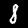
\includegraphics[width=0.1\columnwidth]{pics/MNIST/C3_5.png} 
    & 
\includegraphics[width=0.1\columnwidth]{pics/MNIST/C3_6.png}
    \\
     \rotatebox{90}{$Y_{\cdot 7}$}    
    &  
\includegraphics[width=0.1\columnwidth]{pics/MNIST/C7_1.png} 
    &  
\includegraphics[width=0.1\columnwidth]{pics/MNIST/C7_2.png}
    &  
\includegraphics[width=0.1\columnwidth]{pics/MNIST/C7_3.png}
    & 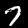
\includegraphics[width=0.1\columnwidth]{pics/MNIST/C7_4.png}
    & 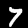
\includegraphics[width=0.1\columnwidth]{pics/MNIST/C7_5.png} 
    & 
\includegraphics[width=0.1\columnwidth]{pics/MNIST/C7_6.png}
    \\ 
    \rotatebox{90}{$Y_{\cdot 9}$}    
    &  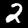
\includegraphics[width=0.1\columnwidth]{pics/MNIST/C9_1.png} 
    &  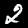
\includegraphics[width=0.1\columnwidth]{pics/MNIST/C9_2.png}
    &  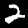
\includegraphics[width=0.1\columnwidth]{pics/MNIST/C9_3.png}
    & 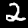
\includegraphics[width=0.1\columnwidth]{pics/MNIST/C9_4.png}
    & 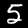
\includegraphics[width=0.1\columnwidth]{pics/MNIST/C9_5.png} 
    & 
\includegraphics[width=0.1\columnwidth]{pics/MNIST/C9_6.png}
    \\ 
  \end{tabular}
  \caption{\textsc{SpectACl} clusters individual handwriting styles instead of cipher shapes.\label{fig:mnist}}
\end{figure}

%====================
% Discussion
%====================
\section{Discussion}
We introduce \textsc{SpectACl} (\emph{Spectral Averagely-dense Clustering}): a new clustering method that combines benefits from spectral clustering and the density-based DBSCAN algorithm, while avoiding some of their drawbacks. 

By computing the spectrum of the weighted adjacency matrix, \textsc{SpectACl} automatically determines the appropriate density for each cluster.  This eliminates the specification of the $minpts$ parameter which is required in DBSCAN, and as we have seen in Figure \ref{fig:intro}, this specification is a serious hurdle for a DBSCAN user to overcome. On two concentric circles with the same number of observations (and hence with different densities), a DBSCAN run with $minpts=25$ lumps all observations into one big cluster.  When increasing $minpts$ by one, DBSCAN jumps to four clusters, none of which are appropriate. \textsc{SpectACl}, conversely, can natively handle these nonconvex clusters with varying densities.

In both spectral clustering and \textsc{SpectACl}, the final step is to postprocess intermediate results with $k$-means. Whether this choice is appropriate for spectral clustering remains open to speculation.  However, from the objective function of \textsc{SpectACl}, we derive an upper bound through the eigenvector decomposition, whose optimization we show to be equal to $k$-means optimization.  Hence, for \textsc{SpectACl}, we demonstrate that this choice for $k$-means postprocessing is mathematically fundamentally sound.

In comparative experiments, competing with DBSCAN, spectral clustering, and robust spectral clustering, we find on synthetic data that the unnormalized version of \textsc{SpectACl} is the most robust to noise (cf.\@ Figure~\ref{fig:noisePlot}), which identifies the appropriate cluster structure in three scenarios while the competitors all fail to do so at least once (cf.\@ Figure~\ref{fig:synthViz}).  On real-life data, \textsc{SpectACl} outperforms the competition on the inherently noisy Pulsar dataset and the Sloan dataset, it performs similarly to spectral clustering on the SNAP dataset, and it is defeated by both spectral clustering and robust spectral clustering on the MNIST dataset (cf.\@ Table~\ref{tbl:realNMI}). The latter observation is explained when looking at the resulting clusters: as Figure~\ref{fig:mnist} illustrates, \textsc{SpectACl} focuses on clusters representing handwriting style rather than clusters representing ciphers, which is not unreasonable behavior for an unsupervised method such as clustering; this uncovered information is merely not reflected in the NMI scores displayed in the table.

Figure~\ref{fig:paramPlot} provides evidence that \textsc{SpectACl} is robust with respect to its parameter settings.  Hence, in addition to its solid foundation in theory and good empirical performance on data, \textsc{SpectACl} provides a clustering method that is easy to use in practice.  Thus, \textsc{SpectACl} is an ideal candidate for outreach beyond data mining experts.

\chapter{Proximal Optimization for Boolean Matrix Factorization}
\label{chap:PALMB}
In a large range of exploratory data mining tasks such as Market Basket Analysis, Text Mining, Collaborative Filtering or DNA Expression Analysis, the data is represented by a binary matrix. As  discussed, a binary representation of the cluster centers is desirable to reflect the binary nature of features. Methods which provide interpretable models in that sense are discussed from the viewpoint of binary matrix factorization, pattern mining, tiling and Boolean matrix factorization~\citep{tatti2012comparing,zimek2015blind}. Of those fields, Boolean matrix factorization is the most flexible one. Boolean factorizations are not required to model partitioning cluster assignments, such as binary matrix factorization and it does not restrict the cluster assignment to the support of a pattern, as is the case in tiling and pattern mining. 
 
Therefore, providing a generic optimization method, solving the problem of~\ref{eq:BoolMF}, has a possible impact on the optimization of all the regarded cluster objectives in Chapter~\ref{chap:ZeroShades}. We have seen that the optimization of non-partitioning clusters is by at large an unsolved problem. Approaches tackling this issue require detailed specifications of parameters which are unknown in advance, such as the amount of overlap and outliers~\citep{whang2017nonCo}. In contrast, we aim at formalizing an optimization scheme which is able to derive the \emph{true} model, regardless of the characteristics of that model; may it be overlapping or not, may it have a large amount of overlap or not. 

%------------FIGURE INTRO SPACE INVADERS-----------
\begin{figure}
  \begin{align*}
      \vcenter{\hbox{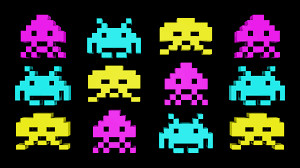
\includegraphics[scale =0.2]{pics/SpaceInv/spaceInv}}} 
      &\approx
      \vcenter{\hbox{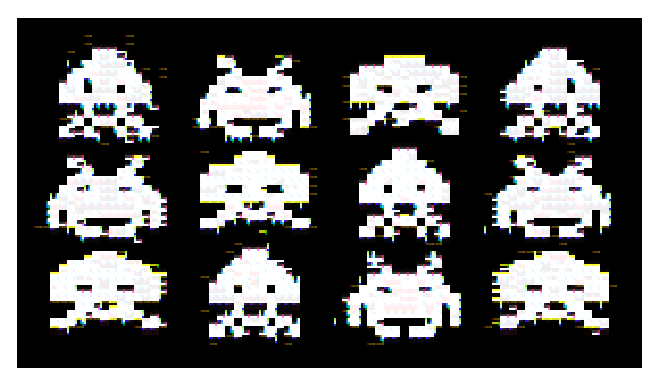
\includegraphics[scale =0.2]{pics/SpaceInv/PandaspaceInv}}}
      = \vcenter{\hbox{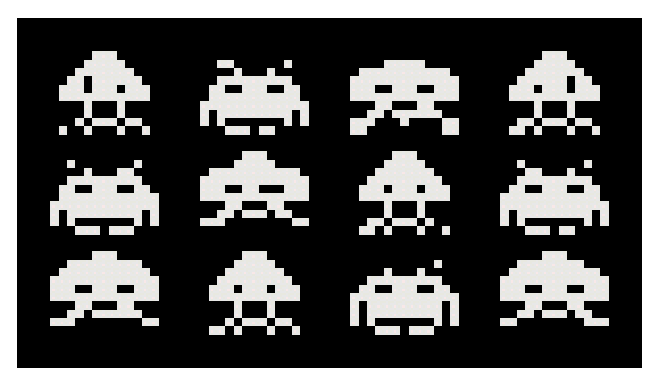
\includegraphics[scale =0.2]{pics/SpaceInv/PandaspaceInv1}}}
     \oplus \vcenter{\hbox{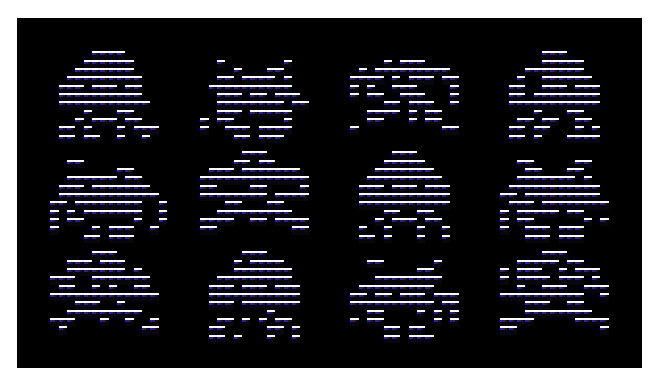
\includegraphics[scale =0.2]{pics/SpaceInv/PandaspaceInv2}}}
     \oplus \vcenter{\hbox{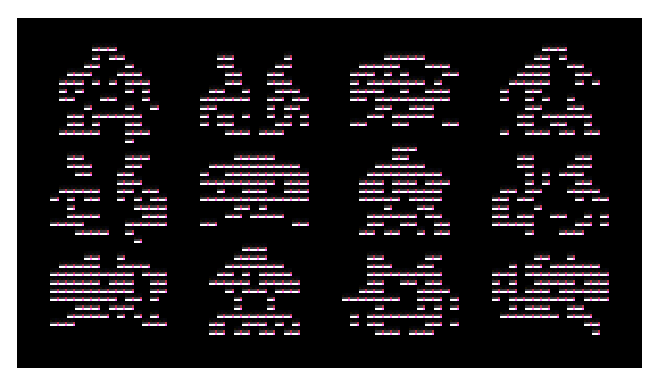
\includegraphics[scale =0.2]{pics/SpaceInv/PandaspaceInv3}}}\\
     \vcenter{\hbox{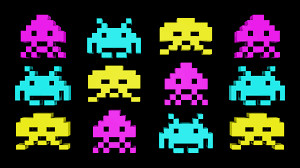
\includegraphics[scale =0.2]{pics/SpaceInv/spaceInv}}}
     &\approx
     \vcenter{\hbox{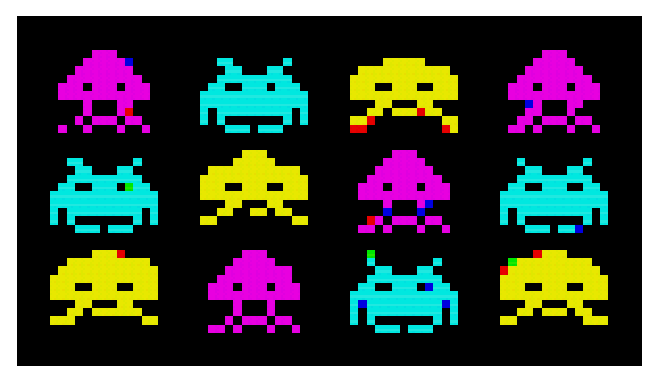
\includegraphics[scale =0.2]{pics/SpaceInv/PrimpSpaceInv}}}
    = \vcenter{\hbox{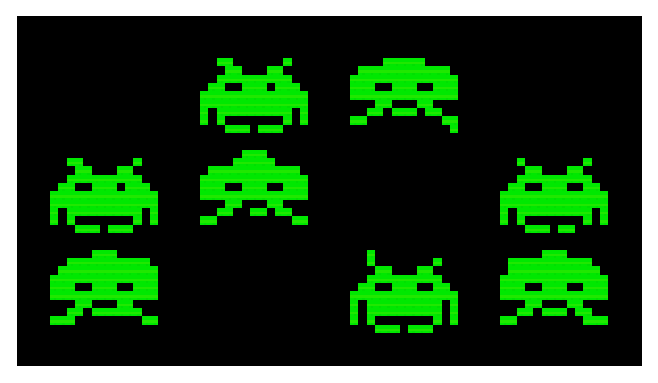
\includegraphics[scale =0.2]{pics/SpaceInv/PrimpSpaceInv1}}}
    \oplus \vcenter{\hbox{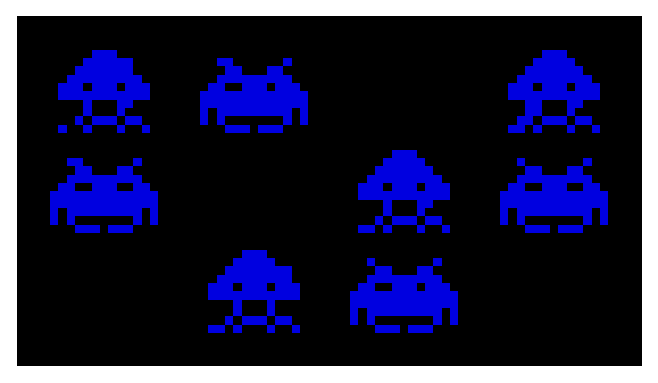
\includegraphics[scale =0.2]{pics/SpaceInv/PrimpSpaceInv2}}}
    \oplus \vcenter{\hbox{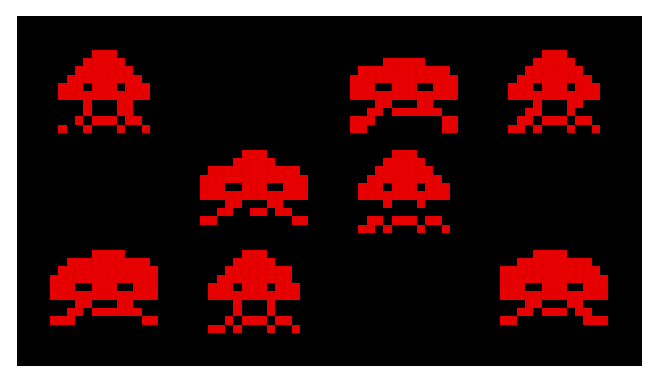
\includegraphics[scale =0.2]{pics/SpaceInv/PrimpSpaceInv3}}}
  \end{align*}
  \caption{Results of a Boolean decomposition of rank three on a picture dataset, depicted on the left. On the top row, the picture is approximated by a greedy approach, on the bottom we display the result of the proposed Proximal optimization scheme for BMF. Best viewed in color.\label{fig:PT:introSpaceInv}}
\end{figure}
Unfortunately, present \ref{eq:BoolMF} employ a greedy heuristic, which can not provide guarantees as known from numerical optimization methods, such as convergence to a local optimum. We make use of an example to show the innate disadvantage, emerging from a strong preference bias of the greedy approach in Figure~\ref{fig:PT:introSpaceInv}. Here, a picture is transformed into a binary data matrix via its binary representation in RGB888 pixel format. On the top row, you see the decomposition obtained by the greedy approach \textsc{Panda+}~\citep{lucchese2014unifying} and on the bottom the approximation derived by the new method which we introduce in this chapter. Each of the three rightmost pictures visualizes an outer product, also called tile in the context of binary factorization. The difference between both results is striking, in particular because the color information gets completely lost in the greedy approximation. We observe that the greedy representation in black and white is attributed to the first outer product being overloaded with the information about shape. Since the color white has a binary representation as a constant one vector, any white pixel in one outer product picture also appears white in the resulting approximation. Accordingly, the greedy approach is very sensitive to making mistakes in the first derived tiles and is therewith also susceptible to noise. In contrast, we propose a simultaneous optimization of the clusters based on a nonnegative relaxation with binary penalization. This approach is similar to the binary factorization by~\cite{zhang2007binary}, employing the mexican hat function for the penalization of nonbinary values (cf.\@ Section~\ref{sec:ZS:Penalty}). However, our method follows latest results in nonconvex optimization theory and provides a general framework for the efficient optimization of matrix factorization under binary constraints. The main contribution of this chapter is the derivation of the proximal mapping, which implements the non-binary penalization. This proximal mapping is usable as a building block to incorporate binary restrictions on one of the matrices in factorization objectives. Known proximal mappings involving other constraints such as nonnegativity, sparseness or the restriction to the probability simplex can then be integrated within the larger optimization framework.  

%=================================================
% Approximating the Boolean Product in Elementary Algebra
%=================================================
\section{Approximating the Boolean Product in Elementary Algebra}
A possible reason for the prevailing usage of heuristics in Boolean matrix factorization is the reasonable belief that relaxations to nonnegative or other  continuous values are not apt to approximate a product in Boolean arithmetic. Contrary to this belief, we argue for the opposite; a nonnegative relaxation is particularly suited to derive overlapping clusterings and is therefore also suited to approximate Boolean matrix factorizations, whose main characteristic is to allow for overlap between the clusters. Now we need to be a bit careful with the word \emph{approximate}. The \ref{eq:BoolMF} problem is NP-hard and NP-hard to aproximate within a constant factor~\citep{miettinen2008discrete}. Hence, we will not be able to produce an efficient algorithm which comes arbitrarily close to the optimal Boolean solution (unless NP=P). Yet we are able to simulate some of the required characteristics of Boolean solutions in a relaxed space. 

%--------- FIGURE OVERLAPPING FACTORIZATION ------------
\begin{figure}
\centering
\begin{align*}
D=
\begin{tikzpicture}[baseline=-0.5ex]
   \matrix [matrix of math nodes,left delimiter=(,right delimiter=),ampersand replacement=\&] (n) {
1\&1\&1\&0 \\
1\&1\&1\&1 \\
0\&1\&1\&1 \\
};
\draw[color=col1,fill=col1,opacity=0.2] (n-1-1.north west) -- (n-1-3.north east) -- (n-2-3.south east) -- (n-2-1.south west) -- (n-1-1.north west);
\draw[color=col2,fill=col2,opacity=0.2] (n-2-2.north west) -- (n-2-4.north east) -- (n-3-4.south east) -- (n-3-2.south west) --(n-2-2.north west);
\end{tikzpicture}
&\approx
%----------------------------
%\\
%----------------------------
\begin{tikzpicture}[baseline=-0.5ex]
   \matrix [matrix of math nodes,left delimiter=(,right delimiter=),ampersand replacement=\&] (n) {
\phantom{.}1\&\phantom{1}.9\&\phantom{1}.9\&.1 \\
.7\&1.2\&1.2\&.7 \\
.1\&\phantom{1}.9\&\phantom{1}.9\&1\phantom{.} \\
};
\draw[color=col1,fill=col1,opacity=0.2] (n-1-1.north west) -- (n-1-3.north east) -- (n-2-3.south east) -- (n-2-1.south west) -- (n-1-1.north west);
\draw[color=col2,fill=col2,opacity=0.2] (n-2-2.north west) -- (n-2-4.north east) -- (n-3-4.south east) -- (n-3-2.south west) --(n-2-2.north west);
\end{tikzpicture}
%---------------------
\\
%---------------------
&\approx
\begin{tikzpicture}[baseline=-0.5ex]
    \matrix [matrix of math nodes,left delimiter=(,right delimiter=),ampersand replacement=\&] (n) {
1\phantom{.}\&0 \\
.6\&.6 \\
0\&1\phantom{.} \\
};
\draw[color=col1,fill=col1,opacity=0.2] (n-1-1.north west) -- (n-1-1.north east) -- (n-2-1.south east) -- (n-2-1.south west) -- (n-1-1.north west);
\draw[color=col2,fill=col2,opacity=0.2] (n-2-2.north west) -- (n-2-2.north east) -- (n-3-2.south east) -- (n-3-2.south west) --(n-2-2.north west);
\end{tikzpicture}
\cdot
\begin{tikzpicture}[baseline=-0.5ex]
    \matrix [matrix of math nodes,left delimiter=(,right delimiter=),ampersand replacement=\&] (n) {
1\&.9\&.9\&.1 \\
.1\&.9\&.9\&1 \\
};
\draw[color=col1,fill=col1,opacity=0.2] (n-1-1.north west) -- (n-1-3.north east) -- (n-1-3.south east) -- (n-1-1.south west) --(n-1-1.north west);
\draw[color=col2,fill=col2,opacity=0.2] (n-2-2.north west) -- (n-2-4.north east) -- (n-2-4.south east) -- (n-2-2.south west) -- (n-2-2.north west);
\end{tikzpicture}
%-------------------------------------
\\
%-----------------------------
D_A=
\begin{tikzpicture}[baseline=-0.5ex]
   \matrix [matrix of math nodes,left delimiter=(,right delimiter=),ampersand replacement=\&] (n) {
1\&1\&1\&0 \\
1\&2\&2\&1 \\
0\&1\&1\&1 \\
};
\draw[color=col1,fill=col1,opacity=0.2] (n-1-1.north west) -- (n-1-3.north east) -- (n-2-3.south east) -- (n-2-1.south west) -- (n-1-1.north west);
\draw[color=col2,fill=col2,opacity=0.2] (n-2-2.north west) -- (n-2-4.north east) -- (n-3-4.south east) -- (n-3-2.south west) --(n-2-2.north west);
\end{tikzpicture}
&=
\mathlarger{\theta}
\begin{tikzpicture}[baseline=-0.5ex]
    \matrix [matrix of math nodes,left delimiter=(,right delimiter=),ampersand replacement=\&] (n) {
1\phantom{.}\&0 \\
.6\&.6 \\
0\&1\phantom{.} \\
};
\draw[color=col1,fill=col1,opacity=0.2] (n-1-1.north west) -- (n-1-1.north east) -- (n-2-1.south east) -- (n-2-1.south west) -- (n-1-1.north west);
\draw[color=col2,fill=col2,opacity=0.2] (n-2-2.north west) -- (n-2-2.north east) -- (n-3-2.south east) -- (n-3-2.south west) --(n-2-2.north west);
\end{tikzpicture}
\cdot \mathlarger{\theta}
\begin{tikzpicture}[baseline=-0.5ex]
    \matrix [matrix of math nodes,left delimiter=(,right delimiter=),ampersand replacement=\&] (n) {
1\&.9\&.9\&.1 \\
.1\&.9\&.9\&1 \\
};
\draw[color=col1,fill=col1,opacity=0.2] (n-1-1.north west) -- (n-1-3.north east) -- (n-1-3.south east) -- (n-1-1.south west) --(n-1-1.north west);
\draw[color=col2,fill=col2,opacity=0.2] (n-2-2.north west) -- (n-2-4.north east) -- (n-2-4.south east) -- (n-2-2.south west) -- (n-2-2.north west);
\end{tikzpicture}
%------------------------------
\\
%------------------------------
D_B=
\begin{tikzpicture}[baseline=-0.5ex]
   \matrix [matrix of math nodes,left delimiter=(,right delimiter=),ampersand replacement=\&] (n) {
1\&1\&1\&0 \\
1\&1\&1\&1 \\
0\&1\&1\&1 \\
};
\draw[color=col1,fill=col1,opacity=0.2] (n-1-1.north west) -- (n-1-3.north east) -- (n-2-3.south east) -- (n-2-1.south west) -- (n-1-1.north west);
\draw[color=col2,fill=col2,opacity=0.2] (n-2-2.north west) -- (n-2-4.north east) -- (n-3-4.south east) -- (n-3-2.south west) --(n-2-2.north west);
\end{tikzpicture}
&=
\mathlarger{\theta}\left(\mathlarger{\theta}
\begin{tikzpicture}[baseline=-0.5ex]
    \matrix [matrix of math nodes,left delimiter=(,right delimiter=),ampersand replacement=\&] (n) {
1\phantom{.}\&0 \\
.6\&.6 \\
0\&1\phantom{.} \\
};
\draw[color=col1,fill=col1,opacity=0.2] (n-1-1.north west) -- (n-1-1.north east) -- (n-2-1.south east) -- (n-2-1.south west) -- (n-1-1.north west);
\draw[color=col2,fill=col2,opacity=0.2] (n-2-2.north west) -- (n-2-2.north east) -- (n-3-2.south east) -- (n-3-2.south west) --(n-2-2.north west);
\end{tikzpicture}
\cdot \mathlarger{\theta}
\begin{tikzpicture}[baseline=-0.5ex]
    \matrix [matrix of math nodes,left delimiter=(,right delimiter=),ampersand replacement=\&] (n) {
1\&.9\&.9\&.1 \\
.1\&.9\&.9\&1 \\
};
\draw[color=col1,fill=col1,opacity=0.2] (n-1-1.north west) -- (n-1-3.north east) -- (n-1-3.south east) -- (n-1-1.south west) --(n-1-1.north west);
\draw[color=col2,fill=col2,opacity=0.2] (n-2-2.north west) -- (n-2-4.north east) -- (n-2-4.south east) -- (n-2-2.south west) -- (n-2-2.north west);
\end{tikzpicture}
\right)
\end{align*}
\caption{Approximation of a binary matrix $D$ with two overlapping tiles (top) applying NMF (second from above) and the factorizations resulting from thresholding the factor matrices to binary matrices in elementary algebra (second from below) and Boolean algebra (below). Tiles are highlighted.}
\label{fig:overlapFact}
\end{figure}
%-------------------------------------------------------
To make our case, we inspect how nonnegative and Boolean matrix factorizations deal with overlapping clusters. An example binary data matrix consisting of two  overlapping tiles and its approximation by a nonnegative matrix factorization is shown in the top two equations of Figure~\ref{fig:overlapFact}. We see that the factors contain values smaller than one at entries which are involved in overlapping parts. With this, overlapping sections are equally well approximated as non-overlapping components. 
The matrices $D_A$ and $D_B$ in Figure~\ref{fig:overlapFact} show the resulting binary and Boolean approximations, thresholding the nonnegative factor matrices at one half. We find that the reconstruction error is largest when the thresholded matrices are multiplied in elementary algebra, as it is the case in binary matrix factorization. In contrast, the fuzzy cluster indication by NMF is suited to indicate a definite clustering with respect to the Boolean algebra. This seems at first contradictory to the discussed near-orthogonality of NMF solutions in Section~\ref{sec:ZS:NMFClus}. However, although NMF has an in-built penalization of nonorthogonal factor matrices (cf.\@ Eq.~\eqref{eq:NMFOrth}), the approximation error is the dominating value of the objective function. Accordingly, the better the factorization approximates the data, implying the higher the rank, the more become solutions of \ref{eq:NMF} orthogonal. Conversely, we conclude that overlap between clusters is mirrored by a nonnegative approximation if the rank is low.   
%==================================
% Proximal Alternating Linearized Minimization
%==================================
\section{Proximal Alternating Linearized Minimization}
Standard gradient descent-based optimization schemes for~\ref{eq:NMF} problems are either multiplicative updates or projected gradient methods. The crucial aspect of both optimization schemes is the determination of the step-size. The optimization with multiplicative updates is slow due to the conservative choice  of the step-size, ensuring that factor matrices are nonnegative. Projected gradient methods often employ a linesearch procedure to determine the optimal step-size, but calculating the optimal step-size in every step is also costly.

\cite{bolte2014proximal} extend optimization results known for convex optimization to the nonconvex case with the \emph{Proximal Alternating Linearized Minimization} (PALM). This technique focuses on objectives breaking down into a smooth part $F$ and a possibly nonsmooth component $\phi$
\begin{align}\label{eq:PalmObj}
 \min_{X,Y}&\	F(X,Y)+ \phi_1(X) +\phi_2(Y) &\text{s.t. }X\in\mathbb{R}^{n\times r}, Y\in\mathbb{R}^{m\times r}.
\end{align}
The function $F$ reflects the objective function with respect to the nonnegative relaxation. We assume for now that $F(X,Y)=\|D-YX^\top\|^2$ returns the approximation error in the Frobenius norm. 
The nonsmooth part $\phi$ may return $\infty$, which can be used to model restrictions of the search space, e.g., the non-negativity constraint of NMF. 
PALM performes an alternating minimization on the linearized objective, substituting $F$ with its first order Taylor approximation. This is achieved by alternating \emph{proximal mappings} from the gradient descent update with respect to $F$, i.e., the following steps are repeated for $1\leq k \leq K$:
\begin{align}\label{eq:PalmIterX}
X_{k+1} &= \prox_{\alpha_k\phi_1}(X_k-\alpha_k\nabla_XF(X_k,Y_k));\\
Y_{k+1} &= \prox_{\beta_k\phi_2}(Y_k-\beta_k\nabla_YF(X_{k+1},Y_k)).\label{eq:PalmIterY}
\end{align}
The proximal mapping of a function $\phi$, is a function which returns a matrix satisfying the following minimization criterion: 
\begin{align}\label{eq:prox}
    \prox_\phi(X) \in \argmin_{X^\star}\left\{\frac{1}{2}\|X-X^\star\|^2+\phi(X^\star)\right\}.
\end{align}
Loosely speaking, the proximal mapping gives its argument a little push into a direction which minimizes $\phi$. For a detailed discussion, see, e.g., \citep{parikh2014proximal}. As we can see in Eqs.~(\ref{eq:PalmIterX}) and (\ref{eq:PalmIterY}), the evaluation of this operator is a base operation. Similarly to the alternating minimization in Eq.~(\ref{eq:als}), finding the minimum of the proximal mapping in every iteration by numerical methods is infeasible in practice. Thus, the trick is to use only simple functions $\phi$ for which the proximal mapping can be calculated in a closed form. 

%------------------------------
% Convergence Results
%-------------------------------
\subsection{Convergence Results}
We state here the main convergence result for PALM in a specified version, requiring that the differentiable part of the objective is smooth and not only continuously differentiable, summarizing the discussion with respect to smooth functions in \citep{bolte2014proximal}. Yet first, we need to introduce some definitions.
\begin{definition}[proper, semi-continuous function] Let $f:\mathbb{R}^{n}\rightarrow (-\infty,\infty]$ be an extended real-valued function. We say $f$ is \emph{proper} if there exists at least one $x\in\mathbb{R}^n$ such that $f(x)<\infty$. The function $f$ is called \emph{lower semi-continuous} if for all $x_0\in\mathbb{R}^n$ the
\[\liminf_{x\rightarrow x_0}f(x)\geq f(x_0).\]
\end{definition}
%------------FIGURE LOWER SEMI-Continuous-----
\begin{figure}
\centering
\begin{tikzpicture}%[scale =0.8]
	\begin{axis}[width=200pt,height = 90pt, axis x line=left, domain=-1:4,ymin=-0.2, axis y line=center, tick align=outside,legend pos=outer north east,legend style={cells={align=left,anchor=west}}]
    	\addplot+[domain=-1:1,mark=none,smooth,col1,ultra thick,samples=100] (\x,\x^2);
    	\addplot+[domain=1:3,mark=none,smooth,col1,ultra thick,samples=100] (\x,{-4*(\x-1.5)^2+4});
        \draw [draw=col1, fill=col1, ultra thick] 
            (axis cs: 1, 1) circle (2.0pt);
    	\draw [draw=col1, fill=white, ultra thick] 
            (axis cs: 1, 3) circle (2.0pt);	
        \addlegendentry{$f(x)=\begin{cases}x^2 & x\leq 1\\ -4(x-1.5)^2+4 & x>1 \end{cases}$\\};
	\end{axis}
\end{tikzpicture}
\caption{A lower semi-continuous function.}
\label{fig:PT:lowerSemiCont}
\end{figure}
The convergence analysis of PALM requires that the nonsmooth part $\phi$ is a proper, lower semi-continuous function. In practice, this is not a demanding requirement.
We display an example of a lower semi-continuous function in Figure~\ref{fig:PT:lowerSemiCont}. Let us exercise what is stated in the definition by this example. The function $f$ has a point of discontinuity at $x=1$. Any limit point of function values $f(x_k)$ for a sequence converging to the point of discontinuity ($x_k\rightarrow 1$) is either equal to one or to three. Thus, we have $\{1,3\}\ni\liminf_{x\rightarrow 1}f(x)\geq f(1)=1$. In other words, lower semi-continuous functions always attain the lowest limit point of function values at a point of discontinuity. The restriction to lower semi-continuous functions $\phi$ ensures inter alia that the prox-operator is well-defined (cf.\@ Eq.~\eqref{eq:prox}).
%-----------
\begin{definition}[Kurdyka-Lojasiewicz functions]
Let $f:\mathbb{R}^{n}\rightarrow \mathbb{R}\cup\{\infty\}$ be a proper lower semi-continuous function and $x_0\in\mathbb{R}^n$, such that\footnote{$\partial $ denotes here the Fr\'{e}chet subdifferential} $\partial f(x_0)\neq\emptyset$. Define a subset of real-valued, continuous functions as
\[\mathcal{K}=\{\kappa:[0,t)\rightarrow \mathbb{R}_+\mid t\in(0,\infty],\kappa(0)=0,\kappa\in C^1(0,t), \kappa\in C^0[0,t)\}.\] 
The function $f$ is said to have the \emph{Kurdyka-{\L}ojasiewicz property} at point $x_0$ if there exists a concave and strictly increasing function $\kappa\in\mathcal{K}$ and an $\epsilon>0$ such that for all 
$x\in \mathcal{N}_\epsilon(x_0)$ satisfying $f(x_0)<f(x)<f(x_0)+t$
the Kurdyka-{\L}ojasiewicz inequality holds for all vectors $g\in\partial f(x)$, that is
\[\kappa^\prime\left(f(x)-f(x_0)\right)\|g\|\geq 1.\]
A function $f$ is called Kurdyka-{\L}ojasiewicz function if it has the Kurdyka-{\L}ojasiewicz property at any point $x_0$ where $\emptyset \neq \partial f$. 
\end{definition}
The impact that a requirement of the Kurdyka-{\L}ojasiewicz property has is not easy to understand. Here, it is only important to know which class of functions satisfy this property and how we can derive for specified functions if they satisfy the Kurdyka-{\L}ojasiewicz property. For this reason, we state some of the general rules from which we can conclude the \KL property for a given function in the following section. The follwoing theorem states the main convergence result for PALM.

\begin{theorem}{{\citep{bolte2014proximal}}}\label{thm:palmConv}
Let $F:\mathbbm{R}^{n\times r}\times \mathbbm{R}^{m\times r}\rightarrow \mathbbm{R}_+$ be a smooth function and let $\phi_1:\mathbbm{R}^{n\times r}\rightarrow [0,\infty]$ and $\phi_2:\mathbbm{R}^{m\times r}\rightarrow [0,\infty]$ be proper and lower semi-continuous functions. Denote with $(\mathcal{X},\mathcal{Y})\subseteq\mathbb{R}^{n\times r}\times \mathbbm{R}^{m\times r}$ the feasible set, defined as
\begin{align*}
    \mathcal{X} = \{X\in \mathbb{R}^{n\times r}\mid \phi_1(X)<\infty\}\quad \text{and} \quad \mathcal{Y} = \{Y\in \mathbb{R}^{n\times r}\mid \phi_2(Y)<\infty\},
\end{align*}
Assume that the following conditions hold:
\begin{enumerate}
\item the partial gradients of $F$ are Lipschitz-continuous, satisfying the following inequality for real-valued functions $M_{\nabla_XF}(Y)$ and $M_{\nabla_XF}(Y)$
\begin{align*}
\|\nabla_XF(X,Y)-\nabla_UF(U,Y)\|&< M_{\nabla_XF}(Y)\|X-U\| &\forall \{X,U\} \subseteq \mathcal{X},\ Y\in\mathcal{Y}\\
\|\nabla_YF(X,Y)-\nabla_VF(X,V)\|&< M_{\nabla_YF}(X)\|Y-V\| &\forall \{Y,V\} \subseteq \mathcal{Y},\ X\in\mathcal{X}
\end{align*}
\item the Lipschitz-moduli are bounded on the feasible set; there exists a constant $M>0$ such that $M_{\nabla_XF}(Y)<M$ and $M_{\nabla_YF}(X)<M$ for all $X\in\mathcal{X}$ and $Y\in\mathcal{Y}$,
\item the function $\Psi(X,Y)=F(X,Y)+\phi_1(X)+\phi_2(Y)$ satisfies the Kurdyka-{\L}ojasiewicz property,
\end{enumerate}
then the sequence $(X_k,Y_k)$ generated by the update rules in Eqs.~\eqref{eq:PalmIterX} and \eqref{eq:PalmIterY}, where the step-sizes are given as
\[\alpha_k=M_{\nabla_XF}(Y_k)^{-1}, \quad \beta_k= M_{\nabla_YF}(X_{k+1})^{-1}.\]
converges to a critical point of the function $\Psi$. 
\end{theorem}
%---------------------------------------
% The Kurdyka-{\L}ojasiewicz Property
%---------------------------------------
\subsection{Kurdyka-{\L}ojasiewicz Property}
Deriving the \KL property on the basis of its definition is hard. luckily, there are some classes of functions, which allow for a more easy derivation of the \KL property. We introduce here the semi-algebraic and definable functions. 
\begin{definition}[Semi-algebraic Sets and Functions]
A set $\mathcal{X}\subseteq \mathbb{R}^n$ is called \emph{semi-algebraic} if it is equal to a finite union $\mathcal{X}=\mathcal{X}_1\cup\ldots\cup\mathcal{X}_k$ of sets
\[\mathcal{X}_l=\{x\in\mathbb{R}^n\mid p_i(x)=0, q_i(x)<0, 1\leq i\leq d\},\]
where $p_i$ and $q_i$ are polynomials.
A function $f:\mathbb{R}^n\rightarrow (-\infty,\infty]$ is called semi-algebraic if its graph $\{(x,f(x))\mid x\in\mathbb{R}^n\}$ is a semi-algebraic set.
\end{definition}
Determining whether a function is semi-algebraic or not does in most cases not require a derivation of the properties according to the definition. Instead, many semi-algebraic functions are composed according to the following rules.
\begin{example}[Semi-algebraic sets and functions]
The following functions are semi-algebraic:
\begin{enumerate}
    \item polynomial functions $p(x)=\sum_{\mathbf{n}\in\mathbb{N}^n}a_\mathbf{n}x^{n_1}\cdot\ldots\cdot x^{n_n}$ where $a_\mathbf{n}\neq 0$ for only finitely many $\mathbf{n}\in\mathbb{N}^n$, 
    \item the sum $\alpha f(x)+\beta g(x)$, product $f(x)g(x)$, division $f(x)/g(x)$ for $g(x)\neq 0$ and composition $f(g(x)$ of semi-algebraic functions $f$ and $g$,
    \item the function $f(x)=\|x\|_p$ for $x\in\mathbb{R}^n$ and $p\geq 0$,
    \item indicator functions of semi-algebraic sets.
\end{enumerate}
\end{example}
Although the class of semi-algebraic functions is large, there are still some very common functions which do not belong to that class, such as the exponential function and the logarithm. For this purpose, we introduce another class of functions, covering the semi-algebraic functions.
\begin{definition}[Definable sets and functions]
The family $\mathcal{O}=\{\mathcal{O}_i\}_{i\in\mathbb{N}}$ of collections of subsets $\mathcal{O}_n\subseteq\mathcal{P}(\mathbb{R}^n)$ is called an o-minimal structure over $\mathbb{R}$ if it satisfies the following axioms:
\begin{enumerate}
    \item $(\mathcal{O}_n,\cup, \cap,\cdot^\complement)$ is a Boolean algebra (cf.\@ Definition~\ref{def:BoolAlgebra})
    \item $A\times\mathbb{R},\mathbb{R}\times A\in\mathcal{O}_{n+1}$ and $\{(x_1,\ldots, x_{n-1})\mid (x_1,\ldots,x_n)\in A\}\in \mathcal{O}_{n}$ for $A\in\mathcal{O}_{n}$ 
    \item $\mathcal{O}_1=\mathcal{I}_1\cup\ldots\cup \mathcal{I}_m$ where $\mathcal{I}_j\in\{(a,b),[a,b],(a,b],[a,b)\},\ a,b\in[-\infty,\infty], m\in\mathbb{N}$ and $\{(x_1,x_2)\in\mathbb{R}^2\mid x_1<x_2\}\in\mathcal{O}_2$
    \item $\{(x_1,\ldots,x_{n-1},x_1)\in\mathbb{R}^n\}\in\mathcal{O}_n$
\end{enumerate}
Given an o-minimal structure $\mathcal{O}$, we call a set $A\subseteq\mathbb{R}^n$ definable if $A\in\mathcal{O}_n$. A function $f:\mathbb{R}^{n}\rightarrow (-\infty,\infty]$ is called definable if its graph is a definable set $\{(x,f(x))\mid x\in\mathbb{R}^n\}\in\mathcal{O}_{n+1}$.
\end{definition}
Similarly like semi-algebraic function, the set of definable functions is closed under most basic operations.
%--------------
\begin{example}[Definable sets and functions]The following functions are definable~\citep{dries1998tame}:
\begin{enumerate}
    \item semi-algebraic functions
    \item the sum $\alpha f(x)+\beta g(x)$, product $f(x)g(x)$, division $f(x)/g(x)$ for $g(x)\neq0$ and composition $f(g(x))$ of definable functions $f$ and $g$
    \item $\exp$ and $\log$
\end{enumerate}
\end{example}
Most importantly, semi-algebraic functions are a subset of definable functions, which are again a subset of the \KL functions.
\begin{theorem}{{\citep{attouch2010proximal}}}
Let $f:\mathbb{R}^n\rightarrow (-\infty,\infty]$ be a proper lower semi-continuous function. If $f$ is definable in an o-minimal structure then it is a Kurdyka-{\L}ojasiewicz function.
\end{theorem}
%=======================
% PALM for BMF
%=======================
\section{PALM for Matrix Factorizations with Binary Constraints}
PALM states no convexity requirements for convergence in Theorem~\ref{thm:palmConv} and is thus suitable for the optimization of a broad class of objective functions. First, we discuss the minimization of the \ref{eq:BoolMF} problem in the framework of PALM, minimizing the approximation error of a Boolean factorization. The overall strategy is to derive a relaxed factorization of approximately binary matrices and to threshold these matrices to binary matrices in the end. Here, we discuss how the approximately binary factorization is derived. 
%-----------------------------------
% A Binary Proximal Mapping
%-----------------------------------
\subsection{A Binary Proximal Mapping}\label{sec:PT:binprox}
While the Mexican hat function can be seen as an $\ell2$ regularization equivalent penalizer for binary values, here, we choose an $\ell1$-equivalent form.
Specifically, we choose $\phi_B(X)=\sum_{i,j}\Lambda(X_{ij})$, which employs the one-dimensional function 
\[
	\Lambda(x) = 
    \begin{cases}
        -|1-2x|+1 &x\in[0,1]\\
        \infty &\text{otherwise}
    \end{cases}
\]
%---------FIGURE LAMBDA------------
\begin{figure}
\centering
\begin{tikzpicture}%[scale =0.8]
	\begin{axis}[width=200pt,height = 90pt, axis x line=left,ymax=1.1, domain=-0.5:1.5, axis y line=center, tick align=outside,legend pos=outer north east,legend entries={$\Lambda(x)$}]
		%\addplot+[mark=none,ultra thick,BlueViolet,smooth] (\x,{10*(0.5*((\x)^2-\x)^2)});
    	\addplot+[domain=0:1,mark=none,smooth,col1,ultra thick,samples=100] (\x,{abs(abs(2*\x-1)-1)});
        \draw[dashed,col1,ultra thick] ({axis cs:1,0}|-{rel axis cs:0,0}) -- ({axis cs:1,0}|-{rel axis cs:0,1});
        \draw[dashed,col1,ultra thick] ({axis cs:0,0}|-{rel axis cs:0,0}) -- ({axis cs:0,0}|-{rel axis cs:0,1});
        \draw [draw=col1, fill=col1, ultra thick] 
            (axis cs: 0, 0) circle (2.0pt);
    	\draw [draw=col1, fill=col1, ultra thick] 
            (axis cs: 1, 0) circle (2.0pt);	
	\end{axis}
\end{tikzpicture}
\caption{The function $\Lambda$ penalizing non-binary values.}
\label{fig:lambda}
\end{figure}
%-----------------------------------
to restrict matrix entries to the interval $[0,1]$ and to penalize non-binary values. As discussed by \cite{zhang2010binary}, restricting the entries of factor matrices between zero and one prevents an imbalance between the factor matrices in which one matrix is very sparse and the other very dense. The curve of $\Lambda$ is depicted  in Fig.~\ref{fig:lambda}. 
%it is semi-algebraic pursuant to the examples of semi-algebraic functions in~\cite{teb14} and through this again a KL function. 
We derive with the following proposition a closed form for the computation of the exact minimum as assigned by the proximal mapping with respect to $\phi_B$. 
\begin{theorem}
Let $\alpha>0$ and $\phi_B(X)=\sum_{i,j}\Lambda(X_{ij})$ for $X\in\R^{m\times n}$. The proximal operator of $\alpha\phi_B$ maps the matrix $X$ to the matrix $\prox_{\alpha\phi_B}(X)=A\in [0,1]^{m\times n}$ defined by $A_{ji}=\prox_{\alpha\Lambda}(X_{ji})$, where for $x\in \R$ it holds that
    \begin{equation}\label{eq:binprox}
	\prox_{\alpha \Lambda}(x)=
    \begin{cases}
        \max\{0,x-2\alpha\} &x\leq0.5\\
        \min\{1,x+2\alpha\} &x>0.5.
    \end{cases}
    \end{equation}
\end{theorem}
\begin{proof}
Let $\alpha>0$, $X\in\R^{m\times n}$ for some $m,n\in\N$ and $A=\prox_{\alpha\phi_B}(X)$. The function $\phi_B$ is fully separable across all matrix entries. In this case, the proximal operator can be applied entry-wise to the composing scalar functions \citep{parikh2014proximal}, i.e., $A_{ji}=\prox_{\alpha\Lambda}(X_{ji})$. It remains to derive the proximal mapping of $\Lambda$ (Eq.~\eqref{eq:binprox}).

The proximal operator reduces to Euclidean projection if the argument lies outside of the function's domain \citep{parikh2014proximal} and it follows that
\[\prox_{\alpha\Lambda}(x)=\theta(x) \text{ if } x\notin[0,1].\]
For $x\in[0,1]$ holds $\Lambda(x)=-|1-2x|+1$ and
\begin{align*}
  \prox_{\alpha\Lambda}(x) &= \argmin_{x^\star\in\R} \left\{\frac{1}{2}(x-x^\star)^2-\alpha|1-2x^\star| +1\alpha\right\}\\
  &= \argmin_{x^\star\in\R} \left\{\underbrace{(x-x^\star)^2-2\alpha|1-2x^\star| +(2\alpha)^2}_{=g(x^\star;x,\alpha)}\right\},
\end{align*}
where $g$ is derived by a multiplication and addition of constants, such that the minimum can easily be derived by completing the square.
\begin{align*}
  g(x^\star;x,\alpha) &=\begin{cases}
    (x-x^\star)^2  -2\alpha(1-2 x^\star) +(2\alpha)^2 & x^\star \leq 0.5\\
    (x-x^\star)^2 +2\alpha(1-2 x^\star) +(2\alpha)^2 & x^\star> 0.5
  \end{cases}\\
  &=
  \begin{cases}
    (x^\star-(x-2\alpha))^2 -2\alpha( 1-2x)& x^\star \leq 0.5\\
    (x^\star-(x+2\alpha))^2 +2\alpha( 1-2x) & x^\star> 0.5
  \end{cases}.
\end{align*}
The function $g$ is a continuous piecewise quadratic function which attains its global minimum at the minimum of one of the two quadratic functions, i.e.,
\[
  \argmin_{x^\star\in\R}g(x^\star;x,\alpha) \in \{x-2\alpha\mid x\leq 0.5+2\alpha\}\cup \{x+2\alpha\mid x> 0.5-2\alpha\}.
\] 
A function value comparison in the intersecting domain $x\in(0.5-2\alpha,0.5+2\alpha]$ yields that
\begin{align*}
g(x-2\alpha;x,\alpha)=-2\alpha(1-2x)\leq g(x+2\alpha;x,\alpha) =2\alpha(1-2x) \Leftrightarrow x\leq 0.5
\end{align*}
%The non-differentiable point $x=0.5$ is not a local minimum as $g(0.5)$ is decreasing along the direction to $x^\star$.
%\qed
\end{proof}
The regularization with $\phi_B$ meets the requirements of the nonsmooth part in an optimization by PALM. 
\begin{lemma}
The function $\phi_B(X)=\sum_{i,s}\Lambda(X_{is})$ is proper, lower semi-continuous and semi-algebraic function.
\end{lemma}
\begin{proof}
the function $f$ is lower semi-continuous, because the function $\Lambda$ is lower semi-continuous. It holds that 
\[\liminf_{x\rightarrow 0}=\liminf_{s\rightarrow 1}=0=f(0)=f(1).\]
Similarly, the semi-algebraic property of $\phi_B$, being a finite sum of function values of $\Lambda$, follows from the semi-algebraic property of $\Lambda(x)$. We write $\Lambda(x)=\delta_{[0,1]}(x)|1-(1-2x)|$, where $\delta_{[0,1]}(x)$ is the indicator function, returning infinity if $x$ is outside of the interval $[0,1]$ and one otherwise. The function $|1-(1-2x)|$ is semi-algebraic as a composition of a polynomial function and the one-norm. The indicator function $\delta_{[0,1]}(x)$ is semi-algebraic if the interval $[0,1]$ is a semi-algebraic set. This is indeed the case according to the definition of semi- algebraic sets, since the interval $[0,1]=\{x\mid p(x)<0\}\cup\{x\mid p(x=0)\}$ for the polynomial function $p(x)=(x-0.5)-0.25$.
\end{proof}
%--------------------------------------
% The General Boolean Matrix Factorization Framework PAL-Tiling 
%--------------------------------------
\subsection{General Boolean Matrix Factorization Framework:  PAL-Tiling }\label{sec:PT:vanillaAlg}
%------ ALG PALTILING -----
\begin{algorithm}[t]
\caption{The proposed general optimization scheme \textsc{PAL-Tiling} for Boolean matrix factorization. The implementation of the function \textsc{Toss}, used in the function \textsc{Round}, specifies which tiles are kept and therefore also when the rank increasing is terminated.}
\begin{algorithmic}[1]
  \Function{PAL-Tiling}{$D;\Delta_r=10$}
    \State $(X_K,Y_K)\gets (\emptyset, \emptyset)$
    \For {$r\in\{\Delta_r,2\Delta_r,3\Delta_r,\ldots\}$}
    \State $(X_0,Y_0) \gets $\Call{IncreaseRank}{$X_K, Y_K,\Delta_r$} \Comment{Append $\Delta_r$ random columns} \label{alg:paltiling:increaseRank}
    \For {$k = 0,1,\ldots$}\label{alg:paltiling:opt} \Comment{Select stopping criterion}
    	\State $\alpha_k^{-1} \gets M_{\nabla_XF}(Y_k)$
        \State $X_{k+1} \gets \prox_{\alpha_k\phi_B}\left(X_k-\alpha_k\nabla_XF(X_k,Y_k)\right)$
       	\State $\beta_k^{-1} \gets M_{\nabla_YF}(X_{k+1})$
        \State $Y_{k+1} \gets \prox_{\beta_k\phi_B}\left(Y_k-\beta_k\nabla_YF(X_{k+1},Y_k)\right)$
    \EndFor
    \State $(X,Y)\gets \Call{Round}{L,X_k,Y_k}$ \Comment{Specify Function \textsc{Toss}} \label{alg:paltiling:round}
    \IIf {$\Call{RankGap}{X,Y,r}$}
    	\textbf{return} $(X,Y)$
    \EndIIf \label{alg:paltiling:rankGap}
    \EndFor
  \EndFunction
  \Statex ~
  \Function{Round}{$L,X_k,Y_k,D$} 
  \State $(X^*,Y^*,L^*)\gets (0,0,\infty)$
  \For {$t_x,t_y\in\{0,0.05,0.1,\ldots 1\}$}
    \State $(X,Y)\gets (\theta_{t_x}(X_k),\theta_{t_y}(Y_k))$
    \For{$s\in\{1,\ldots, r\}$}
        \IIf{\Call{Toss}{$X_{\cdot s},Y_{\cdot s},D$}}  
         $(X_{\cdot s},Y_{\cdot s})\gets (\mathbf{0},\mathbf{0})$ \label{alg:paltiling:toss}
        \EndIIf
    \EndFor
    \IIf{$L(X,Y)< L^*$}
     $(X^*,Y^*,L^*)\gets (X,Y,L(X,Y))$
    \EndIIf
  \EndFor
  \State \textbf{Return} $(X^*,Y^*)$
  \EndFunction
\end{algorithmic}
\label{alg:paltiling}
\end{algorithm}
We sketch our method, the general optimization scheme for Boolean matrix factorizations, called Proximal Alternating Linearized Tiling (\textsc{PAL-Tiling}) in Algorithm~\ref{alg:paltiling}. Given an objective function $L(X,Y)$ having a suitable nonbinary relaxation $F(X,Y)$, satisfying the convergence requirements of PALM concerning the smooth part of the objective, \textsc{PAL-Tiling} computes a Boolean matrix factorization via the nonbinary penalty approach. Our method is suitable to automatically determine the rank of the factorization. We will discuss this feature thoroughly in the following two sections. Here, we state the general scheme, having only the data matrix $D$ and the rank increment $\Delta_r$ as input parameters. The rank determination proceeds as follows: increase the rank until the returned factorization uses fewer tiles than allowed under the provided rank. Decisive for the success or failure of this method is the specification which tiles are used. This depends on the objective function $L(X,Y)$ and the implementation of the function \textsc{Toss} which is invoked in line~\ref{alg:paltiling:toss}.

Let us now go through the algorithm step by step. 
The factor matrices are initialized as empty matrices (having rank zero). At every rank increase, $\Delta_r$ columns of random values between zero and one are appended to the current matrices $(X_K,Y_K)$ in line~\ref{alg:paltiling:increaseRank}. In lines~\ref{alg:paltiling:opt} and \ref{alg:paltiling:round}, the Boolean factorization of rank $r$ is calculated. The function $\phi_B$ is the nonbinary penalization function, which has been defined in the previous Section. After the numerical minimization of the relaxed objective $F(X,Y)$, the matrices $X_K$ and $Y_K$, having entries between zero and one, are rounded to binary matrices $X$ and $Y$ with respect to the Boolean factorization objective $L(X,Y)$. If the rounding procedure returns binary matrices having a rank smaller than $r$, then the current factorization is returned (line~\ref{alg:paltiling:rankGap}). Otherwise, we increase the rank and add $\Delta_r$ random columns to the relaxed solution of the former iteration $(X_K,Y_K)$. Note that our method is not greedy as only the initialization of the factor matrices is based on the result of the former iteration. During the optimization of the relaxed objective, the results of former iterations, employing a smaller rank, might very well be changed.

As a stopping criterion we propose to check whether the average function decrease of the last hundred iterations is smaller than a small threshold. That is, at iteration $k$ we check whether $\nicefrac{1}{500}\sum_{t=k-500}^k(F(X_{t-1},Y_{t-1})-F(X_t,Y_t))<q_K$. How to set the parameter $q_K$ is typically easily inferred from observing the function decrease during the first $10,000$ iterations. For most datasets, a maximum number of ten thousand iterations is appropriate. However, tracing the average function decrease helps to decide when to abort the optimization earlier due to convergence. Throughout this work, we employ a stopping criterion of maximal 50,000 optimization iterations or a minimum average function decrease of $q_K=10^{-4}$.

We also outline the rounding function in Algorithm~\ref{alg:paltiling}. This function basically computes the thresholding parameters $t_x$ and $t_y$ with which the relaxed factor matrices are rounded to binary matrices, such that the objective function $L$ is minimized. However, some some tiles of the binary factorization are tossed according to a specified criterion. Therefore, particular instances of the \textsc{PAL-Tiling} algorithm require the specification of the objective function $L(X,Y)$, its smooth relaxation $F(X,Y)$ together with the corresponding gradient and its Lipschitz moduli $M_{\nabla_XF}(Y)$ and $X_{\nabla_YF}(x)$ and the function $\textsc{Toss}$.

The default objective in Boolean matrix factorization is the minimization of the residual sum of squares as stated in problem~\eqref{eq:BoolMF}. We state the function, gradients and Lipschitz constants, required for the minimization via \textsc{PAL-Tiling} if the rank of the factorization is provided.
%\begin{mybox}
\begin{algSpec}[Vanilla \textsc{PAL-Tiling}]\label{algSpec:BMF}
Apply \textsc{PAL-Tiling} with the following specification of functions:
\begin{align*}
    L(X,Y) &= |D-\theta(YX^\top)| & \textit{(objective)}\\
    F(X,Y)&=\|D-YX^\top\|^2 &\textit{(smooth relaxed part)}\\
    \nabla_XF(X,Y) &= (YX^\top-D)^\top Y &\textit{(partial gradient $X$)}\\
    \nabla_YF(X,Y) &= (YX^\top-D) X &\textit{(partial gradient $Y$)}\\
    M_{\nabla_XF}(Y)&>\|YY^T\|, \quad M_{\nabla_YF}(X)>\|XX^T\| &\textit{(L-moduli)} 
\end{align*}
\end{algSpec}
%\end{mybox}
The stated Lipschitz-moduli are easily derived via the inequality
\begin{align*}
    \|\nabla_XF(X,Y) - \nabla_UF(U,Y)\| &= \|(YX^\top-D)^\top Y - (YU^\top-D)^\top Y\|\\
    &= \|XY^\top Y - UY^\top Y\| \leq \|X-U\|\|Y^\top Y\|.
\end{align*}
The function $F(X,Y)=\sum_{j,i}(D_{ji}-Y_{ j\cdot}X_{\cdot i})^2$ is obviously smooth, because it is a polynomial function. For that reason, $F$ is also a semi-algebraic function.
%-------------------------
\begin{corollary}
The function $F(X,Y)=\|D-YX^\top\|^2$ is smooth and a semi-algebraic function.
\end{corollary}
The implementation of the vanilla \textsc{PAL-Tiling} could be used to optimize a Boolean factorization of a fixed rank. However, here we are particularly interested in an automatic determination of the rank of the factorization. Therefore, we discuss approaches to do so in the following sections, where we evaluate our method in comparison to state-of-the-art Boolean matrix factorization algorithms. 
%======================
% Discussion
%======================
\section{Discussion}
We propose an optimization scheme for the problem of Boolean matrix factorization, based on latest numerical optimization results for nonconvex, objective functions. To this end, we derive a closed form of the proximal mapping with respect to a function which penalizes non-binary values. A thresholding to binary values according to the actual objective function, involving the Boolean product, enables the derivation of factorizations which reflect overlapping clusterings, as desired by Boolean matrix factorization.

The proposed approach has applications to the general problem of matrix factorizations under binary constraints. This class of optimization problems comprises the learning of binary has codes as well. In this scope, \cite{shen2016fast} similarly propose to find optimal hashing codes via PALM. However, in this approach the binary factor matrix denoting the hash codes is strictly constrained to binary values during the optimization by PALM. This is achieved by employing the regularizing function $\phi_\mathbb{B}(X)$ returning zero if the matrix $X$ is binary and returning infinity otherwise. The proximal mapping of the function $\phi_\mathbb{B}$ maps therefore a matrix to the closest binary matrix. Although the resulting optimization with respect to unrelaxed, binary matrices seems desirable at first, we argue that such a procedure is likely to get stuck in local optima which reflect less suitable solutions.  
%\chapter{BMF Rank Selection by Minimum Description Length}
\chaptermark{Rank Selection by MDL}\label{chap:RankMDL}
The possibility to derive a Boolean factorization by means of  numerical optimization methods is a promising theoretically founded alternative to the greedy heuristic, generally applied for \ref{eq:BoolMF} (cf.\@ Section~\ref{sec:ZS:GreedyApproach}). Yet, we also wish to provide a solution to the well researched topic of model selection in Boolean matrix factorization by virtue of \textsc{PAL-Tiling}.  
%one of the most  then we would still face a serious preference bias. This bias concerns the model selection with respect to the number of expected clusters and is generally a crucial question in clustering. However, while the \ref{eq:BoolMF} optimization is not particularly theoretically founded (so far), the determination of the optimal rank in \ref{eq:BoolMF} is. 
However, this objective is difficult to delineate: where to draw the line between structure and noise? One possibility is to apply the \emph{Minimum Description Length} (MDL) principle as proposed by \cite{miettinen2014mdl4bmf} to reduce the considerations into one: exploit just as many regularities as serves the compression of the data. Here, regularities indicate the structural part, 
the similarities between observations which establish a cluster. The description length counterbalances the complexity of the model (the amount of derived clusters) with the fit to the data, measured by the size of the encoded data using the model. Decisive for the feasibility of extracted components is the definition of the encoding. 

\cite{miettinen2014mdl4bmf} evaluate several encodings with respect to their ability to filter a planted structure from noise. Candidate clusters are created by the Boolean matrix factorization \textsc{Asso} and are afterwards selected such that a specified description length is minimized. Another framework proposed by \cite{lucchese2014unifying} greedily selects the clusters which directly minimize the description length. Most recently, \cite{karaev2015getting} propose another greedy scheme with focus on a setting where noise effects more likely flip a one to zero than the other way round. All these methods are capable to identify the underlying clusters in respectively examined settings. By and large, the experiments indicate however that the quality considerably varies depending on the distribution of noise and characteristics of the dataset~\citep{miettinen2014mdl4bmf,karaev2015getting}.  Our main contributions are:
\begin{itemize}
    \item We facilitate the application of the framework \emph{PAL-Tiling} to optimize a description length having an approximation which is suitable for the optimization via PALM, \item we algorithmically integrate the built-in regularization of the model complexity by MDL in order to derive factorizations which do not use more tiles than necessary,
    \item we propose two algorithms as specifications of \textsc{PAL-Tiling}: one applying $\ell 1$-regularization on the matrix factorization (\textsc{Panpal}) and one employing an encoding by code tables as proposed by \cite{siebes2006item} (\textsc{Primp}). 
\end{itemize}
 
%We assess the algorithms' ability to filter the \textit{true} underlying structure from the noise. Therefore, we compare various performance measures in a controlled setting of synthetically generated data as well as for real-world data. We show that \textsc{Primp} is capable of recovering the latent structure in spite of varying database characteristics and noise distributions. In addition, we visualize the derived categorization into clusters by means of images, showing that our conducted minimization procedure of \textit{PAL-Tiling} yields interpretable groupings. 
%=============================
% The MDL Principle
%=============================
\section{MDL Principle}
MDL is introduced by \cite{rissanen1978modeling} as an applicable version of Kolmogorov complexity~\citep{li2008introduction,grunwald2007minimum}.
The learning task to find the best model according to the MDL principle is given by the following minimization problem 
\begin{align*}
    	\min_M&\ L(M) = L^D(M) + L^M(M) &\text{s.t. } M\in\mathcal{M}.
\end{align*} 
The function $L$ denotes the description length, which is composed of the compression size of the database in bits $L^D(M)$ (using model $M$ for the encoding) and description size in bits of the model $M$ itself $L^M(M)$.
Specifications of this task differ in the definition of the encoding which defines in turn the set of considered models $\mathcal{M}$. 
%Typical models for tilings are given by the factorizations which satisfy the constraints
%\[
%	\mathcal{M} = \{(X,Y)\in \{0,1\}^{n\times r}\times\{0,1\}^{m\times r}\mid c(X,Y,N) \leq 0\ \forall c\in \mathcal{C}, r\in\mathcal{R}\}.
%\]
%-----------------------------------
% MDL for itemset compression
%-----------------------------------
\subsection{MDL for Pattern Mining}
The minimum description length is suitable to tackle the problem of pattern explosion, arising in practical applications of pattern mining. The output of frequent pattern mining algorithms is sensitive to the minimum support threshold, defining the meaning of the word \emph{frequent}. If this threshold is set too high, then only a few patterns are returned, reflecting nothing but common knowledge. A small decrease in the minimum support can result however in the output of a vast amount of patterns, whereby most of them are redundant as well. The minimum description length is applicable to select a set of patterns, giving a succinct description all frequent patterns.   

An encoding which is successfully applied in this respect uses code tables  as proposed by~\cite{siebes2006item}. 
The two-columned code table assigns optimal prefix-free codes to a set of patterns: itemsets are listed on the left and assigned codes on the right. Such a dictionary from itemsets to code words can be applied to databases similarly as code words to natural language texts. However, the usage of codes for patterns in a transaction is not as naturally defined as for words in a text. Patterns are not nicely separated by blanks and the possibilities to disassemble a transaction into patterns are numerous. Therefore, we require for every transaction the indication of those patterns  which are used for the transaction's encoding. This is modeled by the function $cover$, which partitions items indicated in a transaction into patterns of the code table. 

Let $CT=\{(\mathcal{X}_s,C_s)|1\leq s\leq r\}$ represent a code table of $r$ patterns $\mathcal{X}_s\subseteq\{1,\ldots,n\}$ and codes $C_s$. Theorem 5.4.1 in \cite{cover2012elements} states that for any distribution $P$ over a finite set $\Omega$, an optimal set of prefix-free codes exists such that the number of required bits for the code of $x\in\Omega$ is approximately
\begin{equation*}
	codelength(x) \approx -\log(P(x)).
\end{equation*}
Desiring that frequently used codes are shorter in size, \cite{siebes2006item} introduce the function $usage$ that maps a pattern to the number of transactions which use it for their cover,
\[usage(\mathcal{X}_s)=|\{j\in\{1,\ldots,m\}\mid \mathcal{X}_s\in cover(CT,D_{j\cdot})\}|.\] 
The probability mass function over all itemsets $\mathcal{X}_s$ in the code table  is defined as
\begin{align}\label{eq:krimpCodeProb}
P(\mathcal{X}_s) = \frac{usage(\mathcal{X}_s)}{\sum_{1\leq t \leq r}usage(\mathcal{X}_t)}.
\end{align}
This implies that $codelength(\mathcal{X}_s)=-\log P(\mathcal{X}_s)$. The data matrix is encoded by a transaction-wise concatenation of codes, denoted by the cover, i.e., transaction $D_{j\cdot}$ is encoded by a concatenation of codes $C_s$ with $\mathcal{X}_s\in cover(CT,D_{j\cdot})$. Therefore, code $C_s$ occurs $usage(\mathcal{X}_s)$ times in the encoded dataset. The size of the data description is then computed as
\begin{align*}
	L^D_{\mathsf{CT}}(CT)
    &=-\sum_{1\leq s\leq r} usage(\mathcal{X}_s) \cdot \log(P(\mathcal{X}_s)).
\end{align*}
The description of the model, the code table, requires the declaration of codes $C_s$ and corresponding patterns $\mathcal{X}_s$. Code $C_s$ has a size of $-\log\left(P(\mathcal{X}_s)\right)$ and a pattern is described by concatenated standard codes of contained items. Standard codes arise from the code table consisting of singleton patterns only, where the usage of singleton $\{i\}$ for $i\in\{1,\ldots,n\}$ is equal to its support $|D_{\cdot i}|$. In conclusion, the description size of the model is computed as  
\begin{align*}
	L_{\mathsf{CT}}^M(CT)
    &= -\sum_{\substack{1\leq s\leq r \\ usage(\mathcal{X}_s)>0}}\left(\log\left(P(\mathcal{X}_s)\right) +\sum_{i\in \mathcal{X}_s}\log\left(\frac{|D_{\cdot i}|}{|D|}\right)\right).
\end{align*}
Note that an efficient computation of the description length employs the possibility to calculate code lengths without realizations of actual codes.
We further remark that the function $L_{\mathsf{CT}}$ originally uses the logarithm with base two. Here, we implicitly reformulate this description length by substituting with the natural logarithm. This is equivalent to multiplying the function by a constant which is negligible during minimization. In return, using the natural logarithm will shorten the derivations in Sec.~\ref{sec:MDL:primp}.

\cite{siebes2006item} use a heuristic cover function in the algorithm \textsc{Krimp} which employs a specified, static order on patterns. For every transaction, the cover function returns a partition of the transaction by the following routine: iterating through all patterns of the code table in the given order, add a pattern to the transactions' cover whenever the transaction supports the pattern. Remove the items belonging to a selected pattern from the transaction and continue the pattern traversion. This way, the usage of a pattern is smaller than or equal to its support.
The determination of patterns contained in the code table is performed by another greedy procedure in \textsc{Krimp}. An input set of frequent patterns -- the code table candidate set -- is traversed in another static order, adding a candidate pattern to the code table whenever that improves the compression size. Additionally, pruning methods are proposed to correct the selection of patterns in the code table.

\textsc{Slim}~\citep{smets2012slim} differs in its candidate generation, which is   dynamically implemented according to an estimated compression gain and dependent on the current code table. This strategy typically improves the compression size, but mainly reduces  the  amount of returned patterns.  
Both approaches consider a vast amount of candidates until the best set of patterns is determined. Time consumption is dominated by computing the usage for each evaluated candidate.
\textsc{SHrimp} \citep{hess2014shrimp} exploits the indexing nature of trees in order to efficiently identify those parts of the database which are affected by an extension of the code table.
\cite{siebes2011structure} restrict with the algorithm \textsc{Groei} the code table to a constant number of patterns. They resort to a heuristic beam search algorithm,
but only for tiny datasets, the beam width parameter can be set to a level allowing a reasonably wide enough exploration of the search space, or else the run time explodes.

All these algorithms follow the heuristic cover definition of \textsc{Krimp} which restricts the usage of a pattern to supporting transactions and prohibits a cover by overlapping patterns. As discussed in the context of tiling (cf.\@ Section~\ref{sec:ZS:BooleanMF}), these restrictions result in less succinct descriptions of the dataset, being susceptible to noise. Correspondingly, there are methods adapting the model selection by minimum description length for Boolean matrix factorization.
%---------------------------
% MDL for BMF
%---------------------------
\subsection{MDL for BMF}
The scheme to employ MDL for rank selection is easily adopted from the one used for pattern mining. 
In every iteration, the description length of the current factorization is compared with the description length from the former iteration, having a lower rank. If the current factorization achieves a lower description length, then another factorization with an increased rank is computed and the procedure repeats itself. Otherwise, the factorization of the former iteration is returned. The performance of this method depends on the algorithm computing the factorization of a given rank and on the encoding which determines the description length.

\cite{lucchese2010noise} propose an encoding reflecting sparse data representations; describing matrices only by their positions of ones. Consequently, the model is described with $L^M_{\ell 1}(X,Y)=|X|+|Y|$ bits and the data with $L^D_{\ell 1}(X,Y)=|D-\theta(YX^\top )|$ bits, up to a multiplicative constant. We denote the resulting description length with $L_{\ell 1}(X,Y)=|D-\theta(YX^\top )|+|X|+|Y|$. The algorithm \textsc{Panda} uses a factorization method which adds a tile (outer product) to the current factorization in a two stage heuristic. 
 
\cite{miettinen2014mdl4bmf} argue that the encoding used in \textsc{Panda} is too coarse. They investigate multiple encodings, applying \textsc{Asso} as Boolean factorization method. Their best-performing encoding is called \emph{Typed XOR DtM} encoding. This is based upon the description of $n$-dimensional binary vectors by number and distribution of ones. 
We refer to  the Typed XOR DtM description length as $L_{\mathsf{TXD}}$ and to the corresponding algorithm as \textsc{Mdl4bmf}. The experimental evaluation suggests that \textsc{Mdl4bmf}'s rank estimation is accurate in a setting with moderate noise, i.e., less than $15\%$, and moderate number of planted tiles, i.e., less than 15. It seems to have a tendency to underfit, as opposed to \textsc{Panda}, which returns on some synthetically generated datasets a rank ten times higher than the actual rank.

On the other hand, the heuristic optimization of \textsc{Panda} is applicaple to any objective function. \cite{lucchese2014unifying} enhance the algorithm \textsc{Panda} to a faster version \textsc{Panda+} and empirically evaluate the ability to detect the \emph{true} clustering via various description lengths and optimization algorithms. In the evaluation with respect to synthetically generated datasets, having less than $10\%$ equally distributed noise, \textsc{Panda+} using the Typed XOR description length $L_{\mathsf{TX}}$ is outperforming any other choice. The performance is explained with the direct minimization of the description length in \textsc{Panda+}, opposed to \textsc{Asso}, minimizing only the residual sum of squares.

Another algorithm which tries to incorporate the direct optimization of the MDL-cost measure is \textsc{Nassau}~\citep{karaev2015getting}. Remarking that the formerly proposed algorithms do not reconsider which clusters have been mined at previous iterations, \textsc{Nassau} refines the whole factorization every few steps, employing \textsc{Asso} for the \ref{eq:BoolMF} optimization. The experiments focus on a setting where noise effects which flip a one to a zero are prevalent. In this case, differences to \textsc{Mdl4bmf} are often hard to capture while \textsc{Nassau} typically outperforms \textsc{Panda+}. 

%===================================
% MDL and PAL-Tiling
%===================================
\section{Minimizing the Description Length in PAL-Tiling}
We wish to derive Boolean factorizations minimizing the description length, hoping that the regularization of the model complexity by the MDL principle is suitable to yield factorizations of an appropriate rank. However, most of the proposed description lengths are not continuous, let alone smooth. Therefore, we need to derive  a smooth relaxation of the description lengths we wish to apply in \textsc{PAL-Tiling}. We assume that there exists a factor $\mu\geq 0$ and regularizing function $G$ such that the smooth relaxation of the description length has the form 
\begin{align}\label{eq:MDL:F}
	F(X,Y)= \frac{\mu}{2}\|D-YX^\top \|^2 + \frac{1}{2} G(X,Y).
\end{align} 
Here, the multiplication with one half refers to the traditional formulation of the residual sum of squares in problem~(\ref{eq:NMF}), which shortens the formulation of gradients. 
In order to meet the convergence criteria of PALM, we require the regularizing function $G$ to be a smooth definable function, having partial gradients which are Lipschitz-continuous with moduli $M_{\nabla_YG}(X)$ and $M_{\nabla_XG}(Y)$, such that
\[\|\nabla_XG(X,Y)-\nabla_UG(U,Y)\|< M_{\nabla_XG}(Y)\|X-U\|,\]
and similarly for $\nabla_YG$. From the triangle inequality follows that the Lipschitz moduli of the partial gradients of $F$ are then given as
\begin{align*}
M_{\nabla_XF}(Y) &= \mu\|YY^\top \| + \frac{1}{2}M_{\nabla_XG}(Y)\\ 
M_{\nabla_YF}(X) &= \mu\|XX^\top \| + \frac{1}{2}M_{\nabla_YG}(X).
\end{align*}
%--- ALG Toss MDL ----
\begin{algorithm}[t]
\caption{The tossing function for the application of \textsc{PAL-Tiling} implementing the determination of the rank via MDL.} 
\begin{algorithmic}[1]
  \Function{Toss}{$x,y,D$}
  	\State \textbf{return} $|x|\leq 1\ \mathsf{OR}\ |y|\leq 1$ 
  \EndFunction
\end{algorithmic}
\label{alg:MDL:toss}
\end{algorithm}
We specify the function \textsc{Toss} in Algorithm~\ref{alg:MDL:toss}, which we employ in the framework of \textsc{PAL-Tiling} to determine the rank via the minimum description length principle. Since the regularization of the model complexity by MDL is supposed to yield factorizations which penalizes tiles reflecting noise effects, we employ a very simplistic function \textsc{Toss}. The function solely decides that singleton tiles, consisting of one row or column, are to be disregarded in the factorization. Therewith, we only need a specification of the description lengths and their relaxed objective for the optimization in \textsc{PAL-Tiling}.
%--------------------------------------
% Panpal
%------------------------------------
\subsection{Panpal}\label{sec:MDL:panpal}
The cost measure $L_{\ell 1}$ (as applied by \textsc{Panda}) is easily  integrated into \textsc{PAL-Tiling}. Since the proximal operator ensures that the factor matrices in all steps are nonnegative, the $\ell 1$-norm of the factor matrices equates a simple summation over all matrix entries. Thus, the $\ell 1$-norm is a smooth function on the nonnegative domain of the factor matrices and can be used as regularizing function. We call the resulting algorithm \textsc{Panpal} as it employs the cost measure of \textsc{Panda} in the minimization technique \textsc{PAL-Tiling}:
%\begin{mybox}
\begin{algSpec}[Panpal] \label{algSpec:panpal}
Apply \textsc{PAL-Tiling} with the function \textsc{Toss} from Algorithm~\ref{alg:MDL:toss} and the following functions:
\begin{align*}
    L(X,Y)&=L_{\ell 1}(X,Y) = |D-\theta(YX^\top )|+|X|+|Y| & \textit{(objective)}\\
    F(X,Y)&=\frac{1}{2}\|D-YX^\top \|^2+ \frac{1}{2}(|X|+|Y|) & \textit{(smooth part)}\\
    \nabla_XF(X,Y,D)&=(YX^\top -D)^\top Y+0.5\mathbf{1}& \textit{(partial gradient X)}\\
\nabla_YF(X,Y,D)&=(YX^\top -D)X+0.5\mathbf{1} & \textit{(partial gradient Y)}\\
M_{\nabla_XF}(Y)&>\|YY^\top \| \quad M_{\nabla_YF}(X)>\|XX^\top \| & \textit{(L-moduli)}
\end{align*}
\end{algSpec}
%\end{mybox}
The smooth relaxation $F$ in \textsc{Panpal} is a polynomial function and thus semi-algebraic. Therefore, the optimization of the relaxed objective of \textsc{Panpal} via PALM converges to a local minimum.
%-------------------------
% primp
%-------------------------
\subsection{Primp}\label{sec:MDL:primp}
So far, the cost measure of \textsc{Krimp} has been disregarded in the context of Boolean matrix factorization. Since the traditionally employed cover function is incompatible with overlapping patterns or patterns which cover more items than persistent in the transaction, the task to find the best encoding by code tables is associated with the sub-domain of pattern mining \citep{miettinen2014mdl4bmf,lucchese2014unifying,karaev2015getting}. The definition of the long-established cover function is heuristically determined under the assumption that there is one globally valid cover function which is applicable on all datasets if a suitable code table is found. Although this approach might be favorable in sub-domains like classification or detection of changes in a data stream \citep{vreeken2011krimp,van2008streamkrimp}, it is current best practice in the domain of Boolean matrix factorization to take negative noise into account (see Section~\ref{sec:ZS:BooleanMF}).  
Thus, we break away from the conventional view on the cover function as a predefined instance and regard it as an extrapolation of the mapping from patterns to transactions which is defined by the matrix $Y$. Thereby, we intend to learn a suitable pair of code table and cover function, tailored to the dataset. This is motivated by the following observation.
%-------------------------------
\begin{restatable}{lemma}{lctbmf}\label{thm:CTBMF}
Let $D$ be a data matrix. For any code table $CT$ and its cover function there exists a Boolean matrix factorization $D=\theta(YX^\top )+N$ such that non-singleton patterns in $CT$ are mirrored in $X$ and the cover function is reflected by $Y$. The description lengths correspond to each other, such that 
\[L_{\mathsf{CT}}(CT)=L_{\mathsf{CT}}(X,Y)=L_{\mathsf{CT}}^D(X,Y)+L_{\mathsf{CT}}^M(X,Y),\]
where the functions returning the model and the data description size are given as  
\begin{align*}
	L_{\mathsf{CT}}^D(X,Y)&=-\sum_{s=1}^r |Y_{\cdot s}| \cdot \log(p_s)
       -\sum_{i=1}^n |N_{\cdot i}| \cdot \log(p_{r+i})
       &=L^D_{\mathsf{CT}}(CT)\\
    L_{\mathsf{CT}}^M(X,Y)
    &=\sum_{s:|Y_{\cdot s}|> 0}\left(X_{\cdot s}^\top \mathbf{c}-\log(p_s)\right)
	+\sum_{i:|N_{\cdot i}|> 0}\left(\mathbf{c}_i-\log(p_{r+i})\right)&=L_{\mathsf{CT}}^M(CT).
\end{align*}
The probabilities $p_s$ and $p_{r+i}$ indicate the relational usage of non-singleton patterns $X_{\cdot s}$ and singletons $\{i\}$,
\[
	p_s = \frac{|Y_{\cdot s}|}{|Y|+|N|},\  p_{r+i} = \frac{|N_{\cdot i}|}{|Y|+|N|}.
\]
We denote with $\mathbf{c}\in\R_+^n$ the vector of standard code lengths for each item, i.e., 
\[\mathbf{c}_i=-\log\left(\frac{|D_{\cdot i}|}{|D|}\right).\]
\end{restatable}
The proof of this lemma can be found in Appendix \ref{chap:AppendixMDL}.
We remark that this formulation also puts new emphasis on the debate about the model definition in this MDL application. As commented by \cite{siebes2011structure}, the cover function actually is a part of the model and if we learn the cover function together with the code table, an encoding of the data is not possible if only the code table is present. 
However, to be in line with common practice in the field we stick with the description length computation as originally proposed by \cite{siebes2006item}, which is also used in Lemma \ref{thm:CTBMF} and makes our results comparable to previously published results.

The transfer from a code table encoding to a Boolean matrix factorization provides another view on the objective of \textsc{Krimp}-related algorithms. While the focus of matrix factorizations lies on the extraction of a given ground truth, the originally formulated task aims at the derivation of subjectively interesting patterns -- equating interestingness with the ability to compress. The non-reducibility requirement in Boolean matrix factorization, returning  linear independent columns of factor matrices and the bound on the rank ($r\leq\min\{m,n\}$) is in alignment with the interpretation of interestingness with compressing abilities.

Considering, in reverse, the transfer from a matrix factorization to an encoding by code tables, we naturally receive access to the treatment of negative noise. The term \emph{negative noise} refers thereby to the decomposition of the data into a factorization and a noise matrix $D=\theta(Y X^\top) +N$. If patterns are not restricted to their support, then the noise matrix $N\in\{-1,0,1\}^{m\times n}$ may take negative values. We can calculate the description size $L_{\mathsf{CT}}(X,Y)$ for arbitrary factor matrices, even if the usage of patterns is not restricted to their support. Yet, the question arises if this also has a suitable interpretation with regard to the encoding. In fact, the interpretation is simple: the items in a transaction having a negative noise entry can be transmitted just as the items with positive noise entries; their singleton codes are appended to the belonging transaction. If the item is not contained in any other pattern used in this transaction, then it corresponds to a positive noise entry and otherwise to a negative. The resulting cover function maps a transaction $D_{j\cdot}$ to the patterns $X_{\cdot s}$ where $Y_{js}=1$ and the singletons $i$ having $N_{ji}\neq 0$.

The compression size $L_{\mathsf{CT}}(X,Y)$ is not continuous. There are points of discontinuity at factorizations where one of the columns of $Y$ or $N$ are zero, that is when a pattern in $X$ or a singleton code is not used at all. We employ a simple hack to fix this issue and assume that each pattern in $X$ is used at least once. For singletons, we do not wish to make such an assumption; usages of singletons indicate errors in the approximation, which we want to keep as small as possible. Therefore, we bound the description length of singleton codes by the approximation error. Then, we obtain a smooth function which meets the requirements of \textsc{PAL-Tiling}. This is specified by the following theorem whose proof can be found in Appendix~\ref{chap:AppendixMDL}. 
%-----------------------------
\begin{restatable}{theorem}{BoundLCT}\label{thm:bound}
Given binary matrices $X$ and $Y$ and $\mu = 1+\log(n)$, it holds that 
\begin{align} \label{eq:approxLN}
		L^D_{\mathsf{CT}}(X,Y) &\leq \mu \|D-YX^\top \|^2-\sum_{s=1}^r(|Y_{\cdot s}|+1)\log\left(\frac{|Y_{\cdot s}|+1}{|Y|+r}\right)+|Y|
\end{align} 
\end{restatable}
This bound encompasses the description size of the data, yet the description size of the model is also discontinuous at points where one of the patterns is not used at all. The description size of one side of the code table, representing the patterns by singleton codes $\mathbf{c}$, has an upper bound of 
\[|X^\top \mathbf{c}|=\sum_{s=1}^rX_{\cdot s}^\top c\geq\sum_{s:|Y_{\cdot s}|>0}X_{\cdot s}^\top c,\] 
which is easily integrated into the smooth approximation. The product $X^\top \mathbf{c}$ returns a nonnegative vector, and thus the the $\ell 1$-norm of this vector boils down to a simple sum over all entries. 
The remaining terms which compose the model complexity are limited upwards by a constant, due to the fixation of the rank during the minimization of the relaxed objective.
Thus, we minimize the relaxed function as denoted in the box below. 
The required Lipschitz constants are computed in Appendix~\ref{chap:AppendixMDL}. We refer to this algorithm as \textsc{Primp}, as it performs \textsc{PAL-Tiling} with the objective of \textsc{Krimp}.   

%\begin{mybox}
\begin{algSpec}[Primp]\label{algSpec:Primp}
Apply \textsc{PAL-Tiling} with the function \textsc{Toss} from Algorithm~\ref{alg:MDL:toss} and the following functions:
\begin{align*}
    c_i&=-\log\left(\frac{|D_{\cdot i}|}{|D|}\right),\quad \mu= 1+\log(n) &\textit{(constants)}\\
    L(X,Y)&= L_{\mathsf{CT}}(X,Y) & \textit{(objective)}\\
    F(X,Y)&=\frac{\mu}{2}\|D-YX^\top \|^2+ \frac{1}{2}G(X,Y) & \textit{(smooth part)}\\
    G(X,Y)&=-\sum_{s=1}^r(|Y_{\cdot s}|+1)\log\left(\frac{|Y_{\cdot s}|+1}{|Y|+r}\right) +|X^\top \mathbf{c}| +|Y|&\\
    \nabla_XF(X,Y)&=\mu(YX^\top -D)^\top Y+\frac{1}{2}\mathbf{c}\mathbf{1}^\top  & \textit{(partial gradient X)}\\
    \nabla_YF(X,Y)&=\mu(YX^\top -D)X-\frac{1}{2}\left(\log\left(\frac{|Y_{\cdot s}|+1}{|Y|+r}\right)-1\right)_{js}& \textit{(partial gradient Y)}\\
    M_{\nabla_X F}(Y)&>\mu\|YY^\top \|\quad M_{\nabla_Y F}(X)>\mu\|XX^\top \|+m & \textit{(L-moduli)}
\end{align*}
\end{algSpec}
%\end{mybox}
The smooth relaxation of Primp is a definable function, because it is a composition of polynomials, division by functions which are not zero and the definable logarithmic function. Therefore, the iterates in the relaxed optimization converge to a local minimum of the relaxed objective.
%=================================
% Experiments
%=================================
\section{Experiments}\label{sec:MDL:Experiments}
We conduct experiments on a series of synthetic data matrices, exploring the ability to detect the planted factorization, i.e., to recover generated matrices X and Y in presence of various noise structures. In real-world data experiments we compare the description lengths of obtained models. Also, we perform a qualitative evaluation of the factor methods, visualizing the algorithms' understanding of tiles and noise on the basis of images. We compare the \textsc{PAL-Tiling} instances \textsc{Panpal} and \textsc{Primp} with the available implementations of 
\textsc{PaNDa+}\footnote{\url{http://hpc.isti.cnr.it/~claudio/web/archives/20131113/index.html}}, \textsc{Mdl4bmf}\footnote{\label{note1}\url{http://people.mpi-inf.mpg.de/~skaraev/}} and \textsc{Nassau}\footnoteref{note1}. For \textsc{Panda+} we choose the TypedXOR measure and use 20 randomization rounds and correlating items as suggested in the literature \citep{lucchese2014unifying}. Apart from that, the default settings apply. 

We exclude \textsc{Slim} from our experiments as it can not be fairly compared to Boolean matrix factorization algorithms. To illustrate, \textsc{Slim} returns far more patterns ($500$ to $3000$ monotonically increasing with noise) than planted (25) in our synthetic data sets. Hence, a depiction of this algorithm's rank would distort the rank charts.

For synthetic and real world experiments, we set the rank increment $\Delta_r=10$; sensitivity to this parameter is explored in Section~\ref{sec:MDL:SynthData}. For our image evaluation, we set (if possible) a maximum number of $10$ returned tiles and depict the four most informative tiles. Here, we set $\Delta_r=1$, to consistently allow for multiple factorization rounds. 

A separate run time comparison of the aforementioned algorithms is not conducted. This is because we can not guarantee that the underlying data structures and platform specific optimizations are equally well tuned, especially for the approaches for which we make use of the reference implementation (\textsc{Panda+}, \textsc{Mdl4bmf} and \textsc{Nassau}). Note, however, that due to the formulation of \textsc{PAL-Tiling} in terms of linear algebra, a highly parallel implementation on graphics processing units (GPU) is straightforward. Therefore, experiments regarding \textsc{Panpal} and \textsc{Primp} are executed on a GPU with 2688 arithmetic cores and 6GiB GDDR5 memory. The run time of the GPU based algorithms is about 50 times lower, compared to the ordinary implementations, e.g., a task that is finished by \textsc{Primp} in a few seconds, requires 30 minutes by \textsc{Mdl4bmf}. We provide the source code of our algorithms together with the data generating script\footnote{\url{http://sfb876.tu-dortmund.de/primp}}.
%-------------------------------
% Synthetic Data Experiments
%-------------------------------
\subsection{Experiments on Synthetic Data} \label{sec:MDL:SynthData}
We generate data matrices according to the scheme established by \cite{miettinen2014mdl4bmf,karaev2015getting} and \cite{lucchese2014unifying}. Yet, we constrain the set of generated factor matrices to contain at least one percent of uniquely assigned ones to ensure linear independence of column vectors. This ensures that for $r^*\leq n,m$ and generated matrices $X^*\in\{0,1\}^{n\times r^*}$ and $Y^*\in\{0,1\}^{m\times r^*}$, the matrix $D=Y^* {X^*}^\top $ indeed has rank $r^*$. We describe the data generation process as a function from dimensions $n$ and $m$, rank $r^*$, density parameter $d$ and noise probabilities $p_+^*$ and $p_-^*$ as stated in Algorithm~\ref{alg:MDL:generateBMF}. 
\begin{algorithm}[t]
\caption{Generation of synthetic datasets for Boolean matrix factorizations.}
\begin{algorithmic}[1]
  \Function{GenerateNoisyBMF}{$n,m,r^*,d,p_+^*,p_-^*$}
  	\State $X^*\gets UniformRand(\{X\in\{0,1\}^{n\times r}\mid 0.01n\leq|X_{\cdot s}|\leq dn\})$
  	\State $Y^*\gets UniformRand(\{Y\in\{0,1\}^{m\times r}\mid 0.01m\leq|Y_{\cdot s}|\leq dm\})$
  	\State $D\gets Y^*\odot {X^*}^\top$
  	\For {$1\leq j\leq m, 1\leq i\leq n$}
%  	    \If{$D_{ji}=1$} 
%  	    \State $D_{ji}=0$ with probability $p_-$ 
%  	    \Else  
%  	    \State $D_{ji}=1$ with probability $p_+$ 
%  	    \EndIf
  	    \State \algorithmicif\ $D_{ji}=1$\ \algorithmicthen\ $D_{ji}\gets 0$ with probability $p_-^*$ 
  	    \State \phantom{\algorithmicif\ $D_{ji}=1$}\ \algorithmicelse\ \ $D_{ji}\gets 1$ with probability $p_+^*$ 
    \EndFor
    \State \textbf{Return} $(X^*,Y^*,D)$
  \EndFunction
\end{algorithmic}
\label{alg:MDL:generateBMF}
\end{algorithm}
We generate datasets for distinct settings with dimensions $(n,m)\in\{(500,1600),\allowbreak(1600,500),\allowbreak(800,1000),\allowbreak(1000,800)\}$, $r\in[5,25]$, $d\in [0.1,0.3]$ and $p_\pm\in [0,0.25]$. 
Table \ref{tbl:statSynthData} summarizes the basic statistics of the generated datasets.   
\begin{table}%[!hp]
	\centering
    %\resizebox{.8\columnwidth}{!}{%
	\begin{tabular}{lrrrrrr}\toprule
Variation & $p_+[\%]$ & $p_-^*[\%]$ & $r$ & $d$ & Density $[\%]$ & Overlap $[\%]$ \\ \midrule
\multirow{2}{*}{Uniform Noise} &
0 & 0 & 25 & 0.1 & $6.6\pm0.8$ & $2.3\pm0.3$\\
& 25 & 25 & 25 & 0.1 & $28.3\pm0.4$ & $2.3\pm0.3$\\ \midrule
\multirow{2}{*}{Pos/Neg Noise} &25 & 3 & 25 & 0.1 & $30.6\pm0.4$ & $3.0\pm0.4$\\
 & 3 & 25 & 25 & 0.1 & $8.5\pm0.4$ & $2.9\pm0.5$\\ \midrule
\multirow{2}{*}{Rank} & 10 & 10 & 5 & 0.1 &  $11.3\pm0.4$ & $0.3\pm0.2$\\
 & 10 & 10 & 45 & 0.1 & $18.6\pm0.9$ & $8.7\pm1.0$\\ \midrule
\multirow{2}{*}{Density} & 10 & 10 & 25 & 0.1 & $15.3\pm0.6$ & $2.3\pm0.3$\\
 & 10 & 10 & 25 & 0.3 & $40.6\pm4.3$ & $26.9\pm6.1$\\\bottomrule
\end{tabular}
\caption{Characteristics of generated datasets. The values are aggregated over eight generated datasets, four for each combination of dimensions $(n,m)\in\{(500,1600),(800,1000)\}$. Overlap denotes the percentage of overlapping entries in relation to the region covered by all tiles together and density is the region covered by all tiles together in relation to $nm$.}\label{tbl:statSynthData}
\end{table}
%----------------------------------------
% Measuring the Tiling Quality
%----------------------------------------
%\subsection{Measuring the Tiling Quality}\label{sec:MDL:Eval}

\paragraph{Evaluation}
We quantify how well a computed clustering $(X,Y)$  matches the planted clustering $(X^*,Y^*)$ by the $\mathsf{F}$-measure, as proposed in Section~\ref{sec:SA:synthExp}.
We assume w.l.o.g.\@ that $X,X^*\in\{0,1\}^{n\times r}$ and $Y,Y^*\in\{0,1\}^{n\times r}$, otherwise we attach zero columns to the matrices such that the dimensions match. We require the following substitutions of precision and recall, in order to take the selection of features in a tile into account:
\begin{align*}
	\pre(s,t) &= \frac{|(Y^*_{\cdot s}\circ Y_{\cdot t})(X^*_{\cdot s}\circ X_{\cdot t})^\top |}{|Y_{\cdot t}X_{\cdot t}^\top |} &\quad 
    \rec(s,t) &= \frac{|(Y^*_{\cdot s}\circ Y_{\cdot t})(X^*_{\cdot s}\circ X_{\cdot t})^\top |}{|Y^*_{\cdot s}{X^*_{\cdot s}}^\top |}. 
\end{align*}
Accordingly, the calculation of precision and recall for the whole factorization is adapted such that
\begin{align*}
\pre &= \frac{\sum_{s=1}^r|(Y^*_{\cdot s}\circ Y_{\cdot \sigma(s)})(X^*_{\cdot s}\circ X_{\cdot \sigma(s)})^\top |}{\sum_{s=1}^r|Y_{\cdot s}X_{\cdot s}^\top |} 
= \frac{|(Y^*\circ Y_{\cdot \sigma(\cdot)})(X^*\circ X_{\cdot \sigma(\cdot)})^\top |}{|YX^\top |}\\ 
\rec &= \frac{\sum_{s=1}^r|(Y^*_{\cdot s}\circ Y_{\cdot \sigma(s)})(X^*_{\cdot s}\circ X_{\cdot \sigma(s)})^\top |}{\sum_{s=1}^r|Y_{\cdot s}^* {X_{\cdot s}^*}^\top |} 
    = \frac{|(Y^*\circ Y_{\cdot\sigma(\cdot)})(X^*\circ X_{\cdot \sigma(\cdot)})^\top |}{|Y^*{X^*}^\top |}.
\end{align*}
The plots which display the $\mathsf{F}$-measure indicate the average value with error bars having the length of twice the standard deviation.
We furthermore express the values of involved cost measures in relation to the empty model
\[
	\%F(X,Y) = \frac{F(X,Y)}{F(\mathbf{0},\mathbf{0})}\cdot 100.
\]
%----------------------------
% Make some Noise
%----------------------------
\paragraph{Make some Noise}
In the following series of experiments, varying the noise, we plot the $\mathsf{F}$-measure and the rank of the returned Boolean factorization against the percentage of noise which is added. The planted factorization has a rank of $r^*=25$ and density parameter $d=0.1$. The noise level varies from $0\%$ to $25\%$ as displayed on the $x$-axis.  
%---------FIGURE NOISE 800x1000------------
\begin{figure}
\centering
\begin{filecontents}{Panda_n800m1000F.dat}
x y std
0 0.762 0.22
5 0.914 0.15
10 0.98 0.03
15 0.901 0.16
20 0.855 0.07
25 0.16 0.07
\end{filecontents}
\begin{filecontents}{Panda_n800m1000R.dat}
x y std
0 23.4 1.71
5 24.5 1.35
10 24.3 0.82
15 23.2 1.69
20 18.4 3.63
25 1.1 0.32
\end{filecontents}
\begin{filecontents}{superPimpLam4_n800m1000F.dat}
x y std
0 0.9993000000000001 0.0
5 0.9991999999999999 0.0
10 0.9960000000000001 0.0
15 0.9872 0.0
20 0.9692000000000001 0.0
25 0.9089 0.02
\end{filecontents}
\begin{filecontents}{superPimpLam4_n800m1000R.dat}
x y std
0 25.4 0.52
5 25.6 0.7
10 29.6 2.91
15 33.3 1.83
20 34.2 3.22
25 36.9 6.26
\end{filecontents}
\begin{filecontents}{nmfL1Lam2_n800m1000F.dat}
x y std
0 0.9190000000000002 0.02
5 0.9053000000000001 0.06
10 0.7759 0.04
15 0.8127000000000001 0.08
20 0.7596999999999999 0.06
25 0.5826 0.07
\end{filecontents}
\begin{filecontents}{nmfL1Lam2_n800m1000R.dat}
x y std
0 16.1 1.45
5 16.6 3.27
10 9.6 1.9
15 11.3 2.5
20 9.8 1.99
25 7.7 1.83
\end{filecontents}
\begin{filecontents}{Nassau_n800m1000F.dat}
x y std
0 1.0 0.0
5 0.999 0.0
10 0.962 0.01
15 0.867 0.03
20 0.432 0.1
25 0.1 0.05
\end{filecontents}
\begin{filecontents}{Nassau_n800m1000R.dat}
x y std
0 25.0 0.0
5 25.0 0.0
10 21.6 1.9
15 17.3 2.36
20 7.1 1.52
25 1.3 0.48
\end{filecontents}
\begin{filecontents}{Mdl4bmf_n800m1000F.dat}
x y std
0 1.0 0.0
5 0.988 0.0
10 0.934 0.02
15 0.824 0.03
20 0.696 0.03
25 0.48 0.07
\end{filecontents}
\begin{filecontents}{Mdl4bmf_n800m1000R.dat}
x y std
0 25.0 0.0
5 25.6 0.7
10 24.2 2.82
15 21.0 2.16
20 14.7 2.21
25 8.8 1.55
\end{filecontents}
\begin{filecontents}{Panda_n1000m800F.dat}
x y std
0 0.666 0.23
5 0.705 0.19
10 0.857 0.16
15 0.86 0.16
20 0.561 0.31
25 0.177 0.04
\end{filecontents}
\begin{filecontents}{Panda_n1000m800R.dat}
x y std
0 24.6 2.32
5 23.3 1.49
10 24.1 0.99
15 23.1 1.91
20 10.5 7.93
25 1.2 0.42
\end{filecontents}
\begin{filecontents}{superPimpLam4_n1000m800F.dat}
x y std
0 0.9997 0.0
5 0.9955999999999999 0.0
10 1.0 0.0
15 0.9984 0.0
20 0.9892 0.0
25 0.9397 0.02
\end{filecontents}
\begin{filecontents}{superPimpLam4_n1000m800R.dat}
x y std
0 25.2 0.42
5 25.9 0.74
10 25.0 0.0
15 24.9 0.32
20 24.1 1.1
25 21.5 3.6
\end{filecontents}
\begin{filecontents}{nmfL1Lam2_n1000m800F.dat}
x y std
0 0.9343 0.02
5 0.9550999999999998 0.03
10 0.8512000000000001 0.07
15 0.8643000000000001 0.04
20 0.7451000000000001 0.07
25 0.5422 0.09
\end{filecontents}
\begin{filecontents}{nmfL1Lam2_n1000m800R.dat}
x y std
0 17.9 2.42
5 19.4 2.01
10 13.3 2.11
15 13.5 1.84
20 9.1 1.85
25 7.7 1.83
\end{filecontents}
\begin{filecontents}{Nassau_n1000m800F.dat}
x y std
0 0.988 0.02
5 0.196 0.15
10 0.156 0.23
15 0.0 0.0
20 0.0 0.0
25 0.0 0.0
\end{filecontents}
\begin{filecontents}{Nassau_n1000m800R.dat}
x y std
0 25.2 1.48
5 4.0 3.16
10 2.3 2.5
15 0.0 0.0
20 0.0 0.0
25 0.0 0.0
\end{filecontents}
\begin{filecontents}{Mdl4bmf_n1000m800F.dat}
x y std
0 1.0 0.0
5 0.991 0.0
10 0.933 0.03
15 0.833 0.04
20 0.711 0.02
25 0.515 0.04
\end{filecontents}
\begin{filecontents}{Mdl4bmf_n1000m800R.dat}
x y std
0 25.0 0.0
5 25.0 0.82
10 23.8 1.14
15 21.8 2.49
20 15.8 1.93
25 8.7 0.95
\end{filecontents}
%---------------------------
% F MEASURE UNIFORM NOISE (LEFT-ABOVE)
%---------------------------
\begin{tikzpicture}[baseline]  
		\begin{axis}[
        	axis lines = left,
			title={$D\in\{0,1\}^{800\times1000}$},
            height=.33\linewidth,
            width=.5\linewidth, 
			ylabel={$\mathsf{F}$},
			xmax=25.5, ymin=0, ymax=1.1
			]
            \addplot+[cPrimp,mark options ={cPrimp},mark repeat={3}, thick, error bars/.cd,y dir = both, y explicit]  table[x=x,y=y,y error=std] {superPimpLam4_n800m1000F.dat}; 
            \addplot+[cPan,mark options ={cPan},mark repeat={3}, thick, error bars/.cd,y dir = both, y explicit]  table[x=x,y=y,y error=std] {nmfL1Lam2_n800m1000F.dat};
            \addplot+[cPanda,dashed,mark options ={cPanda},mark repeat={3}, thick, error bars/.cd,y dir = both, y explicit]  table[x=x,y=y,y error=std] {Panda_n800m1000F.dat}; 
            \addplot+[cNassau,dashed,mark options ={cNassau},mark repeat={3}, thick, error bars/.cd,y dir = both, y explicit]  table[x=x,y=y,y error=std] {Nassau_n800m1000F.dat}; 
           \addplot+[cMdl4bmf,dashed,mark options ={cMdl4bmf},mark repeat={3}, thick, error bars/.cd,y dir = both, y explicit]  table[x=x,y=y,y error=std] {Mdl4bmf_n800m1000F.dat};
		\end{axis} 
\end{tikzpicture}
%---------------------------
% F MEASURE NEGATIVE NOISE (MIDDLE-ABOVE)
%---------------------------
\begin{tikzpicture}[baseline]  
		\begin{axis}[
        	title={$D^T\in\{0,1\}^{1000\times800}$},
        	axis lines = left,
            height=.33\linewidth,
            width=.5\linewidth,
			xmax=25.5, ymin=0, ymax=1.1
			]
            \addplot+[cPrimp,mark options ={cPrimp},mark repeat={3}, thick, error bars/.cd,y dir = both, y explicit]  table[x=x,y=y,y error=std] {superPimpLam4_n1000m800F.dat}; 
            \addplot+[cPan,mark options ={cPan},mark repeat={3}, thick, error bars/.cd,y dir = both, y explicit]  table[x=x,y=y,y error=std] {nmfL1Lam2_n1000m800F.dat};
            \addplot+[cPanda,dashed,mark options ={cPanda},mark repeat={3}, thick, error bars/.cd,y dir = both, y explicit]  table[x=x,y=y,y error=std] {Panda_n1000m800F.dat};
            \addplot+[cNassau,dashed,mark options ={cNassau},mark repeat={3}, thick, error bars/.cd,y dir = both, y explicit]  table[x=x,y=y,y error=std] {Nassau_n1000m800F.dat}; 
           \addplot+[cMdl4bmf,dashed,mark options ={cMdl4bmf},mark repeat={3}, thick, error bars/.cd,y dir = both, y explicit]  table[x=x,y=y,y error=std] {Mdl4bmf_n1000m800F.dat};
		\end{axis} 
\end{tikzpicture}
%---------------------------
% RANK(X,Y) UNIFORM NOISE (LEFT-BELOW) 
%---------------------------
\begin{tikzpicture}[baseline]  
		\begin{axis}[
        	axis lines = left,
            height=.33\linewidth,
            width=.5\linewidth,
			xlabel={$p_+=p_-\ [\%]$},     
			ylabel={$r$},
			xmax=25.5, xmin=0, ymin=0, ymax=40.2
			]
            \addplot+[cPrimp,mark options ={cPrimp},mark repeat={3}, thick, error bars/.cd,y dir = both, y explicit]  table[x=x,y=y,y error=std] {superPimpLam4_n800m1000R.dat}; 
            \addplot+[cPan,mark options ={cPan},mark repeat={3}, thick, error bars/.cd,y dir = both, y explicit]  table[x=x,y=y,y error=std] {nmfL1Lam2_n800m1000R.dat};
            \addplot+[cPanda,dashed,mark options ={cPanda},mark repeat={3}, thick, error bars/.cd,y dir = both, y explicit]  table[x=x,y=y,y error=std] {Panda_n800m1000R.dat};
            \addplot+[cNassau,dashed,mark options ={cNassau},mark repeat={3}, thick, error bars/.cd,y dir = both, y explicit]  table[x=x,y=y,y error=std] {Nassau_n800m1000R.dat}; 
           \addplot+[cMdl4bmf,dashed,mark options ={cMdl4bmf},mark repeat={3}, thick, error bars/.cd,y dir = both, y explicit]  table[x=x,y=y,y error=std] {Mdl4bmf_n800m1000R.dat};
		\end{axis} 
\end{tikzpicture}
%---------------------------
% RANK(X,Y) NEGATIVE NOISE (MIDDLE BELOW)
%---------------------------
\begin{tikzpicture}[baseline]  
		\begin{axis}[
        	axis lines = left,
            height=.33\linewidth,
            width=.5\linewidth,
			xlabel={$p_+=p_-\ [\%]$},    
			xmax=25.5, xmin=0, ymin=0, ymax=40.2,
            legend columns =-1,
            legend entries={Primp,Panpal,Panda+,Nassau,Mdl4bmf},
            legend to name=labelMDLNoise8_10
			]
            \addplot+[cPrimp,mark options ={cPrimp},mark repeat={3}, thick, error bars/.cd,y dir = both, y explicit]  table[x=x,y=y,y error=std] {superPimpLam4_n1000m800R.dat}; 
            \addplot+[cPan,mark options ={cPan},mark repeat={3}, thick, error bars/.cd,y dir = both, y explicit]  table[x=x,y=y,y error=std] {nmfL1Lam2_n1000m800R.dat};
            \addplot+[cPanda,dashed,mark options ={cPanda},mark repeat={3}, thick, error bars/.cd,y dir = both, y explicit]  table[x=x,y=y,y error=std] {Panda_n1000m800R.dat};
            \addplot+[cNassau,dashed,mark options ={cNassau},mark repeat={3}, thick, error bars/.cd,y dir = both, y explicit]  table[x=x,y=y,y error=std] {Nassau_n1000m800R.dat}; 
           \addplot+[cMdl4bmf,dashed,mark options ={cMdl4bmf},mark repeat={3}, thick, error bars/.cd,y dir = both, y explicit]  table[x=x,y=y,y error=std] {Mdl4bmf_n1000m800R.dat};
		\end{axis} 
\end{tikzpicture}
\\

\pgfplotslegendfromname{labelMDLNoise8_10}
\caption{Variation of uniform noise for $800\times 1000$ and $1000\times 800$ dimensional data. Comparison of $\mathsf{F}$-measures (the higher the better) and the estimated rank of the calculated Boolean factorization (the closer to 25 the better) for varying levels of noise, i.e., $p_+^*=p_-^*$ is indicated on the x-axis (best viewed in color).}
\label{fig:noise810}
\end{figure}
%-----------------------------------
%---------FIGURE NOISE 1600x500------------
\begin{figure}
\centering
\begin{filecontents}{Panda_n1600m500F.dat}
x y std
0 0.535 0.18
5 0.582 0.17
10 0.653 0.19
15 0.719 0.24
20 0.523 0.32
25 0.121 0.03
\end{filecontents}
\begin{filecontents}{Panda_n1600m500R.dat}
x y std
0 23.5 1.43
5 24.8 1.14
10 24.5 1.43
15 20.9 3.6
20 8.7 6.22
25 1.0 0.0
\end{filecontents}
\begin{filecontents}{superPimpLam4_n1600m500F.dat}
x y std
0 0.9987 0.0
5 0.9993000000000001 0.0
10 0.9979000000000001 0.0
15 0.9914999999999999 0.01
20 0.9677999999999999 0.02
25 0.8629 0.07
\end{filecontents}
\begin{filecontents}{superPimpLam4_n1600m500R.dat}
x y std
0 25.7 0.67
5 25.2 0.63
10 25.2 0.42
15 24.0 0.82
20 21.0 2.62
25 15.8 3.12
\end{filecontents}
\begin{filecontents}{nmfL1Lam2_n1600m500F.dat}
x y std
0 0.9538 0.02
5 0.9289 0.07
10 0.8401 0.05
15 0.7579999999999999 0.17
20 0.58 0.16
25 0.24450000000000002 0.17
\end{filecontents}
\begin{filecontents}{nmfL1Lam2_n1600m500R.dat}
x y std
0 19.4 2.55
5 18.5 3.6
10 12.8 1.69
15 10.7 2.06
20 8.1 0.74
25 5.0 2.16
\end{filecontents}
\begin{filecontents}{Nassau_n1600m500F.dat}
x y std
0 0.0 0.0
5 0.0 0.0
10 0.0 0.0
15 0.0 0.0
20 0.0 0.0
25 0.0 0.0
\end{filecontents}
\begin{filecontents}{Nassau_n1600m500R.dat}
x y std
0 0.0 0.0
5 0.0 0.0
10 0.0 0.0
15 0.0 0.0
20 0.0 0.0
25 0.0 0.0
\end{filecontents}
\begin{filecontents}{Mdl4bmf_n1600m500F.dat}
x y std
0 1.0 0.0
5 0.984 0.01
10 0.926 0.03
15 0.844 0.02
20 0.722 0.05
25 0.541 0.06
\end{filecontents}
\begin{filecontents}{Mdl4bmf_n1600m500R.dat}
x y std
0 25.0 0.0
5 24.9 0.88
10 22.1 1.45
15 16.7 3.53
20 13.3 2.91
25 9.1 1.37
\end{filecontents}
\begin{filecontents}{Panda_n500m1600F.dat}
x y std
0 0.814 0.21
5 0.776 0.23
10 0.906 0.16
15 0.896 0.13
20 0.822 0.1
25 0.252 0.11
\end{filecontents}
\begin{filecontents}{Panda_n500m1600R.dat}
x y std
0 23.7 2.21
5 24.0 1.33
10 24.1 0.74
15 23.5 1.84
20 17.9 4.04
25 2.0 1.25
\end{filecontents}
\begin{filecontents}{superPimpLam4_n500m1600F.dat}
x y std
0 0.9994 0.0
5 0.9999 0.0
10 0.9993000000000001 0.0
15 0.9957 0.0
20 0.9802000000000002 0.01
25 0.9224 0.02
\end{filecontents}
\begin{filecontents}{superPimpLam4_n500m1600R.dat}
x y std
0 24.8 0.42
5 25.8 0.63
10 25.0 0.0
15 24.7 0.48
20 23.4 1.17
25 20.5 3.17
\end{filecontents}
\begin{filecontents}{nmfL1Lam2_n500m1600F.dat}
x y std
0 0.8344999999999999 0.06
5 0.7868 0.06
10 0.7615000000000001 0.05
15 0.7421 0.08
20 0.6948 0.12
25 0.41529999999999995 0.11
\end{filecontents}
\begin{filecontents}{nmfL1Lam2_n500m1600R.dat}
x y std
0 12.4 1.84
5 9.8 1.32
10 9.0 0.0
15 8.7 0.67
20 7.9 1.2
25 5.2 1.48
\end{filecontents}
\begin{filecontents}{Nassau_n500m1600F.dat}
x y std
0 0.887 0.19
5 0.589 0.16
10 0.531 0.07
15 0.616 0.16
20 0.458 0.08
25 0.176 0.09
\end{filecontents}
\begin{filecontents}{Nassau_n500m1600R.dat}
x y std
0 25.6 1.07
5 21.5 2.59
10 17.9 2.81
15 15.2 2.62
20 8.1 1.73
25 2.4 1.35
\end{filecontents}
\begin{filecontents}{Mdl4bmf_n500m1600F.dat}
x y std
0 1.0 0.0
5 0.989 0.0
10 0.932 0.02
15 0.838 0.03
20 0.673 0.05
25 0.444 0.07
\end{filecontents}
\begin{filecontents}{Mdl4bmf_n500m1600R.dat}
x y std
0 25.0 0.0
5 25.7 0.48
10 22.2 1.81
15 19.4 2.17
20 13.4 1.51
25 8.0 2.4
\end{filecontents}
%---------------------------
% F MEASURE UNIFORM NOISE (LEFT-ABOVE)
%---------------------------
\begin{tikzpicture}[baseline]  
		\begin{axis}[
        	axis lines = left,
			title={$D\in\{0,1\}^{500\times1600}$},
            height=.33\linewidth,
            width=.5\linewidth, 
			ylabel={$\mathsf{F}$},
			xmax=25.5, ymin=0, ymax=1.1
			]
            \addplot+[cPrimp,mark options ={cPrimp},mark repeat={3}, thick, error bars/.cd,y dir = both, y explicit]  table[x=x,y=y,y error=std] {superPimpLam4_n500m1600F.dat}; 
            \addplot+[cPan,mark options ={cPan},mark repeat={3}, thick, error bars/.cd,y dir = both, y explicit]  table[x=x,y=y,y error=std] {nmfL1Lam2_n500m1600F.dat};
            \addplot+[cPanda,dashed,mark options ={cPanda},mark repeat={3}, thick, error bars/.cd,y dir = both, y explicit]  table[x=x,y=y,y error=std] {Panda_n500m1600F.dat}; 
            \addplot+[cNassau,dashed,mark options ={cNassau},mark repeat={3}, thick, error bars/.cd,y dir = both, y explicit]  table[x=x,y=y,y error=std] {Nassau_n500m1600F.dat}; 
           \addplot+[cMdl4bmf,dashed,mark options ={cMdl4bmf},mark repeat={3}, thick, error bars/.cd,y dir = both, y explicit]  table[x=x,y=y,y error=std] {Mdl4bmf_n500m1600F.dat};
		\end{axis} 
\end{tikzpicture}
%---------------------------
% F MEASURE NEGATIVE NOISE (MIDDLE-ABOVE)
%---------------------------
\begin{tikzpicture}[baseline]  
		\begin{axis}[
        	title={$D^\top\in\{0,1\}^{1600\times500}$},
        	axis lines = left,
            height=.33\linewidth,
            width=.5\linewidth,
			xmax=25.5, ymin=0, ymax=1.1
			]
            \addplot+[cPrimp,mark options ={cPrimp},mark repeat={3}, thick, error bars/.cd,y dir = both, y explicit]  table[x=x,y=y,y error=std] {superPimpLam4_n1600m500F.dat}; 
            \addplot+[cPan,mark options ={cPan},mark repeat={3}, thick, error bars/.cd,y dir = both, y explicit]  table[x=x,y=y,y error=std] {nmfL1Lam2_n1600m500F.dat};
            \addplot+[cPanda,dashed,mark options ={cPanda},mark repeat={3}, thick, error bars/.cd,y dir = both, y explicit]  table[x=x,y=y,y error=std] {Panda_n1600m500F.dat};
            \addplot+[cNassau,dashed,mark options ={cNassau},mark repeat={3}, thick, error bars/.cd,y dir = both, y explicit]  table[x=x,y=y,y error=std] {Nassau_n1600m500F.dat}; 
           \addplot+[cMdl4bmf,dashed,mark options ={cMdl4bmf},mark repeat={3}, thick, error bars/.cd,y dir = both, y explicit]  table[x=x,y=y,y error=std] {Mdl4bmf_n1600m500F.dat};
		\end{axis} 
\end{tikzpicture}
%---------------------------
% RANK(X,Y) UNIFORM NOISE (LEFT-BELOW) 
%---------------------------
\begin{tikzpicture}[baseline]  
		\begin{axis}[
        	axis lines = left,
            height=.33\linewidth,
            width=.5\linewidth,
			xlabel={$p_+^*=p_-^*\ [\%]$},     
			ylabel={$r$},
			xmax=25.5, xmin=0, ymin=0, ymax=40.2
			]
            \addplot+[cPrimp,mark options ={cPrimp},mark repeat={3}, thick, error bars/.cd,y dir = both, y explicit]  table[x=x,y=y,y error=std] {superPimpLam4_n500m1600R.dat}; 
            \addplot+[cPan,mark options ={cPan},mark repeat={3}, thick, error bars/.cd,y dir = both, y explicit]  table[x=x,y=y,y error=std] {nmfL1Lam2_n500m1600R.dat};
            \addplot+[cPanda,dashed,mark options ={cPanda},mark repeat={3}, thick, error bars/.cd,y dir = both, y explicit]  table[x=x,y=y,y error=std] {Panda_n500m1600R.dat};
            \addplot+[cNassau,dashed,mark options ={cNassau},mark repeat={3}, thick, error bars/.cd,y dir = both, y explicit]  table[x=x,y=y,y error=std] {Nassau_n500m1600R.dat}; 
           \addplot+[cMdl4bmf,dashed,mark options ={cMdl4bmf},mark repeat={3}, thick, error bars/.cd,y dir = both, y explicit]  table[x=x,y=y,y error=std] {Mdl4bmf_n500m1600R.dat};
		\end{axis} 
\end{tikzpicture}
%---------------------------
% RANK(X,Y) NEGATIVE NOISE (MIDDLE BELOW)
%---------------------------
\begin{tikzpicture}[baseline]  
		\begin{axis}[
        	axis lines = left,
            height=.33\linewidth,
            width=.5\linewidth,
			xlabel={$p_+^*=p_-^*\ [\%]$},    
			xmax=25.5, xmin=0, ymin=0, ymax=40.2,
            legend columns =-1,
            legend entries={Primp,Panpal,Panda+,Nassau,Mdl4bmf},
            legend to name=labelMDLNoise5_16
			]
            \addplot+[cPrimp,mark options ={cPrimp},mark repeat={3}, thick, error bars/.cd,y dir = both, y explicit]  table[x=x,y=y,y error=std] {superPimpLam4_n1600m500R.dat}; 
            \addplot+[cPan,mark options ={cPan},mark repeat={3}, thick, error bars/.cd,y dir = both, y explicit]  table[x=x,y=y,y error=std] {nmfL1Lam2_n1600m500R.dat};
            \addplot+[cPanda,dashed,mark options ={cPanda},mark repeat={3}, thick, error bars/.cd,y dir = both, y explicit]  table[x=x,y=y,y error=std] {Panda_n1600m500R.dat};
            \addplot+[cNassau,dashed,mark options ={cNassau},mark repeat={3}, thick, error bars/.cd,y dir = both, y explicit]  table[x=x,y=y,y error=std] {Nassau_n1600m500R.dat}; 
           \addplot+[cMdl4bmf,dashed,mark options ={cMdl4bmf},mark repeat={3}, thick, error bars/.cd,y dir = both, y explicit]  table[x=x,y=y,y error=std] {Mdl4bmf_n1600m500R.dat};
		\end{axis} 
\end{tikzpicture}
\\

\pgfplotslegendfromname{labelMDLNoise5_16}
\caption{Variation of uniform noise for $500\times 1600$ and $1600\times 500$ dimensional data. Comparison of $\mathsf{F}$-measures (the higher the better) and the estimated rank of the calculated Boolean factorization (the closer to 25 the better) for varying levels of noise, i.e., $p_+^*=p_-^*$ is indicated on the x-axis (best viewed in color).}
\label{fig:noise516}
\end{figure}
%-----------------------------------

First, we compare the effects of the matrix dimensions and aggregate results over 10 generated matrices with dimensions $800\times 1000$ and $500\times 1600$ together with their transpose, as depicted in Figures~\ref{fig:noise810} and \ref{fig:noise516}. Comparing the results for a data matrix and its transpose is particularly interesting for the algorithm \textsc{Primp}. Since the description length of code table encoding applies different regularizations on $X$ and $Y$, we want to asses how transposition affects \textsc{Primp}'s results in practice. The remaining algorithms minimize an objective which is invariant to a transposition of the input matrix. It is desirable that this is also reflected in practice.

We observe from Figures~\ref{fig:noise810} and \ref{fig:noise516} that the algorithms likely return fewer tiles the more the noise increases. This culminates in the replication of almost none of the clusters at highest noise level for the algorithms \textsc{Panda+} and \textsc{Nassau}. \textsc{Nassau} particularly strongly underestimates the rank if the data matrix is transposed. That is, if the input matrix is more wide than tall then \textsc{Nassau} returns only a few tiles, if any, even if the noise is low. \textsc{Panda+} yields correct rank estimations up to a noise of $15\%$, but its fluctuating $\mathsf{F}$-measure indicates that planted tiles are not correctly recovered after all. In particular, its $\mathsf{F}$-values  differ from the untransposed to the transposed case even if the rank estimations are approximately correct. \textsc{Mdl4bmf} shows a robust behavior towards a transposition of the input matrix. Its suitable rank estimations up to a noise of $15\%$ are mirrored in a high $\mathsf{F}$-measure. \textsc{Panpal} consistently underestimates the rank, yet achieves comparatively high $\mathsf{F}$-measures. The results exhibit minor deviations from the untransposed to the transposed case, which become more recognizable when $n$ and $m$ deviate further from each other (Figure~\ref{fig:noise516}) and the noise level is low. Under these circumstances, \textsc{Panpal} yields  higher rank estimations if the matrix is transposed. We note, that  the code of \textsc{PAL-Tiling} and therewith also the code of \textsc{Panpal} inhibits only one distinction between  $X$ and $Y$, which is the order in which gradient steps are invoked. Apparently, this influences the sparseness of the resulting factor matrices. Unfortunately, a thorough examination of this effect is beyond the scope of this work.  
\textsc{Primp} is characterized by overall high values in the $\mathsf{F}$-measure. It has a tendency to estimate the rank higher in the untransposed case, that is if the input matrix is more tall than wide. This is particularly notable if the  matrices are almost square (Figure~\ref{fig:noise810}). That aside, the overall high $\mathsf{F}$-measure shows that additionally modeled clusters cover only a small area in comparison to planted ones. 

%---------FIGURE NOISE POS AND NEG------------
\begin{figure}
\centering
\begin{filecontents}{PandaPosF.dat}
x y std
0 0.615 0.22
5 0.658 0.21
10 0.847 0.2
15 0.862 0.18
20 0.94 0.13
25 0.989 0.01
\end{filecontents}
\begin{filecontents}{PandaPosR.dat}
x y std
0 23.375 2.0
5 23.5 1.41
10 23.875 1.25
15 23.875 1.46
20 23.25 1.04
25 23.5 1.2
\end{filecontents}
\begin{filecontents}{superPimpLam4PosF.dat}
x y std
0 0.999 0.0
5 0.99925 0.0
10 0.998875 0.0
15 0.998625 0.0
20 0.9955 0.0
25 0.9885 0.0
\end{filecontents}
\begin{filecontents}{superPimpLam4PosR.dat}
x y std
0 25.375 0.74
5 25.625 0.74
10 26.375 2.88
15 26.0 1.93
20 26.875 4.36
25 27.0 4.66
\end{filecontents}
\begin{filecontents}{nmfL1Lam2PosF.dat}
x y std
0 0.903875 0.07
5 0.892625 0.11
10 0.8785 0.09
15 0.82025 0.09
20 0.78825 0.12
25 0.745875 0.15
\end{filecontents}
\begin{filecontents}{nmfL1Lam2PosR.dat}
x y std
0 16.375 3.07
5 16.25 5.28
10 14.75 3.77
15 11.75 3.15
20 11.375 3.66
25 10.625 3.46
\end{filecontents}
\begin{filecontents}{NassauPosF.dat}
x y std
0 1.0 0.0
5 0.894 0.2
10 0.697 0.28
15 0.451 0.06
20 0.385 0.02
25 0.294 0.07
\end{filecontents}
\begin{filecontents}{NassauPosR.dat}
x y std
0 25.0 0.0
5 24.25 1.49
10 18.625 3.81
15 14.125 1.96
20 9.875 1.36
25 6.0 0.93
\end{filecontents}
\begin{filecontents}{Mdl4bmfPosF.dat}
x y std
0 1.0 0.0
5 0.991 0.0
10 0.942 0.01
15 0.866 0.03
20 0.745 0.07
25 0.617 0.06
\end{filecontents}
\begin{filecontents}{Mdl4bmfPosR.dat}
x y std
0 25.0 0.0
5 25.5 0.53
10 24.375 1.51
15 22.0 1.77
20 17.875 1.64
25 16.25 2.43
\end{filecontents}
\begin{filecontents}{PandaNegF.dat}
x y std
0 0.627 0.14
5 0.676 0.22
10 0.781 0.21
15 0.674 0.14
20 0.76 0.19
25 0.676 0.07
\end{filecontents}
\begin{filecontents}{PandaNegR.dat}
x y std
0 22.625 2.0
5 24.875 0.99
10 24.5 1.07
15 24.375 1.6
20 24.5 1.07
25 23.75 1.75
\end{filecontents}
\begin{filecontents}{superPimpLam4NegF.dat}
x y std
0 0.99875 0.0
5 0.999 0.0
10 0.996875 0.0
15 0.9958750000000001 0.0
20 0.9973749999999999 0.0
25 0.994375 0.0
\end{filecontents}
\begin{filecontents}{superPimpLam4NegR.dat}
x y std
0 25.5 0.76
5 25.5 1.07
10 25.625 0.74
15 25.875 1.13
20 25.875 0.83
25 26.375 1.06
\end{filecontents}
\begin{filecontents}{nmfL1Lam2NegF.dat}
x y std
0 0.935 0.04
5 0.8871249999999999 0.05
10 0.891875 0.1
15 0.8675 0.09
20 0.8145 0.09
25 0.8479999999999999 0.09
\end{filecontents}
\begin{filecontents}{nmfL1Lam2NegR.dat}
x y std
0 18.875 2.9
5 17.0 1.85
10 16.875 3.6
15 15.125 3.04
20 13.5 4.81
25 14.375 3.58
\end{filecontents}
\begin{filecontents}{NassauNegF.dat}
x y std
0 0.867 0.25
5 0.917 0.15
10 1.0 0.0
15 1.0 0.0
20 1.0 0.0
25 0.999 0.0
\end{filecontents}
\begin{filecontents}{NassauNegR.dat}
x y std
0 23.5 2.98
5 24.875 0.35
10 25.0 0.0
15 25.0 0.0
20 25.0 0.0
25 25.0 0.0
\end{filecontents}
\begin{filecontents}{Mdl4bmfNegF.dat}
x y std
0 0.999 0.0
5 0.998 0.0
10 0.997 0.0
15 0.997 0.0
20 0.995 0.0
25 0.993 0.0
\end{filecontents}
\begin{filecontents}{Mdl4bmfNegR.dat}
x y std
0 25.125 0.35
5 25.125 0.35
10 25.25 0.46
15 25.0 0.0
20 25.25 0.46
25 25.0 0.0
\end{filecontents}
\begin{filecontents}{superPimpLam4UniF.dat}
x y std
0 0.998625 0.0
5 0.999375 0.0
10 0.9994999999999999 0.0
15 0.9926249999999999 0.01
20 0.978625 0.01
25 0.899 0.05
\end{filecontents}
\begin{filecontents}{superPimpLam4UniR.dat}
x y std
0 25.375 0.92
5 25.25 0.46
10 25.375 0.74
15 26.75 4.5
20 25.75 4.1
25 25.125 7.9
\end{filecontents}
\begin{filecontents}{nmfL1Lam2UniF.dat}
x y std
0 0.9161250000000001 0.05
5 0.864375 0.1
10 0.7569999999999999 0.1
15 0.7506249999999999 0.12
20 0.610125 0.17
25 0.35475 0.2
\end{filecontents}
\begin{filecontents}{nmfL1Lam2UniR.dat}
x y std
0 17.75 2.76
5 16.0 4.24
10 10.875 2.36
15 10.625 2.13
20 8.5 1.93
25 4.75 2.05
\end{filecontents}
\begin{filecontents}{PandaUniF.dat}
x y std
0 0.802375 0.24
5 0.7648750000000001 0.24
10 0.9337499999999999 0.13
15 0.9754999999999998 0.01
20 0.651625 0.28
25 0.143875 0.11
\end{filecontents}
\begin{filecontents}{PandaUniR.dat}
x y std
0 24.5 1.2
5 24.125 1.46
10 24.375 1.19
15 23.75 1.49
20 12.875 8.27
25 1.25 1.16
\end{filecontents}
\begin{filecontents}{NassauUniF.dat}
x y std
0 0.925375 0.14
5 0.76875 0.25
10 0.8172499999999999 0.21
15 0.714125 0.19
20 0.407125 0.1
25 0.0995 0.05
\end{filecontents}
\begin{filecontents}{NassauUniR.dat}
x y std
0 24.625 1.06
5 22.625 2.67
10 20.375 2.83
15 15.5 2.33
20 6.875 2.59
25 1.375 0.52
\end{filecontents}
\begin{filecontents}{Mdl4bmfUniF.dat}
x y std
0 1.0 0.0
5 0.990875 0.0
10 0.930875 0.01
15 0.826 0.03
20 0.6585000000000001 0.05
25 0.458125 0.08
\end{filecontents}
\begin{filecontents}{Mdl4bmfUniR.dat}
x y std
0 25.0 0.0
5 25.0 0.76
10 24.125 2.1
15 20.5 3.21
20 15.125 2.23
25 8.75 2.38
\end{filecontents}
%---------------------------
% F MEASURE UNIFORM NOISE (LEFT-ABOVE)
%---------------------------
\begin{tikzpicture}[baseline]  
		\begin{axis}[
        	axis lines = left,
			title={Uniform Noise},
            height=.33\linewidth,
            width=.34\linewidth, 
			ylabel={$\mathsf{F}$},
			xmax=25.2, ymin=0, ymax=1.1
			]
            \addplot+[cPrimp,mark options ={cPrimp},mark repeat={3}, thick, error bars/.cd,y dir = both, y explicit]  table[x=x,y=y,y error=std] {superPimpLam4UniF.dat}; 
            \addplot+[cPan,mark options ={cPan},mark repeat={3}, thick, error bars/.cd,y dir = both, y explicit]  table[x=x,y=y,y error=std] {nmfL1Lam2UniF.dat};
            \addplot+[cPanda,dashed,mark options ={cPanda},mark repeat={3}, thick, error bars/.cd,y dir = both, y explicit]  table[x=x,y=y,y error=std] {PandaUniF.dat}; 
            \addplot+[cNassau,dashed,mark options ={cNassau},mark repeat={3}, thick, error bars/.cd,y dir = both, y explicit]  table[x=x,y=y,y error=std] {NassauUniF.dat}; 
           \addplot+[cMdl4bmf,dashed,mark options ={cMdl4bmf},mark repeat={3}, thick, error bars/.cd,y dir = both, y explicit]  table[x=x,y=y,y error=std] {Mdl4bmfUniF.dat};
		\end{axis} 
\end{tikzpicture}
%---------------------------
% F MEASURE NEGATIVE NOISE (MIDDLE-ABOVE)
%---------------------------
\begin{tikzpicture}[baseline]  
		\begin{axis}[
        	title={Negative Noise},
        	axis lines = left,
            height=.33\linewidth,
            width=.34\linewidth,
			xmax=25.5, ymin=0, ymax=1.1
			]
            \addplot+[cPrimp,mark options ={cPrimp},mark repeat={3}, thick, error bars/.cd,y dir = both, y explicit]  table[x=x,y=y,y error=std] {superPimpLam4NegF.dat}; 
            \addplot+[cPan,mark options ={cPan},mark repeat={3}, thick, error bars/.cd,y dir = both, y explicit]  table[x=x,y=y,y error=std] {nmfL1Lam2NegF.dat};
            \addplot+[cPanda,dashed,mark options ={cPanda},mark repeat={3}, thick, error bars/.cd,y dir = both, y explicit]  table[x=x,y=y,y error=std] {PandaNegF.dat};
            \addplot+[cNassau,dashed,mark options ={cNassau},mark repeat={3}, thick, error bars/.cd,y dir = both, y explicit]  table[x=x,y=y,y error=std] {NassauNegF.dat}; 
           \addplot+[cMdl4bmf,dashed,mark options ={cMdl4bmf},mark repeat={3}, thick, error bars/.cd,y dir = both, y explicit]  table[x=x,y=y,y error=std] {Mdl4bmfNegF.dat};
		\end{axis} 
\end{tikzpicture}
%---------------------------
% F MEASURE POSITIVE NOISE (RIGHT-ABOVE) 
%---------------------------
\begin{tikzpicture}[baseline]  
		\begin{axis}[
        	axis lines = left,
			title={Positive Noise},
            height=.33\linewidth,
            width=.33\linewidth, 
			xmax=25.2, ymin=0, ymax=1.1
			]
            \addplot+[cPrimp,mark options ={cPrimp},mark repeat={3}, thick, error bars/.cd,y dir = both, y explicit]  table[x=x,y=y,y error=std] {superPimpLam4PosF.dat}; 
            \addplot+[cPan,mark options ={cPan},mark repeat={3}, thick, error bars/.cd,y dir = both, y explicit]  table[x=x,y=y,y error=std] {nmfL1Lam2PosF.dat};
            \addplot+[cPanda,dashed,mark options ={cPanda},mark repeat={3}, thick, error bars/.cd,y dir = both, y explicit]  table[x=x,y=y,y error=std] {PandaPosF.dat};
            \addplot+[cNassau,dashed,mark options ={cNassau},mark repeat={3}, thick, error bars/.cd,y dir = both, y explicit]  table[x=x,y=y,y error=std] {NassauPosF.dat}; 
           \addplot+[cMdl4bmf,dashed,mark options ={cMdl4bmf},mark repeat={3}, thick, error bars/.cd,y dir = both, y explicit]  table[x=x,y=y,y error=std] {Mdl4bmfPosF.dat};
		\end{axis} 
\end{tikzpicture}
%---------------------------
% RANK(X,Y) UNIFORM NOISE (LEFT-BELOW) 
%---------------------------
\begin{tikzpicture}[baseline]  
		\begin{axis}[
        	axis lines = left,
            height=.33\linewidth,
            width=.35\linewidth,
			xlabel={$p_+=p_-\ [\%]$},     
			ylabel={$r$},
			xmax=25.2, xmin=0, ymin=0, ymax=40.2
			]
            \addplot+[cPrimp,mark options ={cPrimp},mark repeat={3}, thick, error bars/.cd,y dir = both, y explicit]  table[x=x,y=y,y error=std] {superPimpLam4UniR.dat}; 
            \addplot+[cPan,mark options ={cPan},mark repeat={3}, thick, error bars/.cd,y dir = both, y explicit]  table[x=x,y=y,y error=std] {nmfL1Lam2UniR.dat};
            \addplot+[cPanda,dashed,mark options ={cPanda},mark repeat={3}, thick, error bars/.cd,y dir = both, y explicit]  table[x=x,y=y,y error=std] {PandaUniR.dat};
            \addplot+[cNassau,dashed,mark options ={cNassau},mark repeat={3}, thick, error bars/.cd,y dir = both, y explicit]  table[x=x,y=y,y error=std] {NassauUniR.dat}; 
           \addplot+[cMdl4bmf,dashed,mark options ={cMdl4bmf},mark repeat={3}, thick, error bars/.cd,y dir = both, y explicit]  table[x=x,y=y,y error=std] {Mdl4bmfUniR.dat};
		\end{axis} 
\end{tikzpicture}
%---------------------------
% RANK(X,Y) NEGATIVE NOISE (MIDDLE BELOW)
%---------------------------
\begin{tikzpicture}[baseline]  
		\begin{axis}[
        	axis lines = left,
            height=.33\linewidth,
            width=.35\linewidth,
			xlabel={$p_-\ [\%]\ (p_+=3\%)$},    
			xmax=25.2, xmin=0, ymin=0, ymax=40.2
			]
            \addplot+[cPrimp,mark options ={cPrimp},mark repeat={3}, thick, error bars/.cd,y dir = both, y explicit]  table[x=x,y=y,y error=std] {superPimpLam4NegR.dat}; 
            \addplot+[cPan,mark options ={cPan},mark repeat={3}, thick, error bars/.cd,y dir = both, y explicit]  table[x=x,y=y,y error=std] {nmfL1Lam2NegR.dat};
            \addplot+[cPanda,dashed,mark options ={cPanda},mark repeat={3}, thick, error bars/.cd,y dir = both, y explicit]  table[x=x,y=y,y error=std] {PandaNegR.dat};
            \addplot+[cNassau,dashed,mark options ={cNassau},mark repeat={3}, thick, error bars/.cd,y dir = both, y explicit]  table[x=x,y=y,y error=std] {NassauNegR.dat}; 
           \addplot+[cMdl4bmf,dashed,mark options ={cMdl4bmf},mark repeat={3}, thick, error bars/.cd,y dir = both, y explicit]  table[x=x,y=y,y error=std] {Mdl4bmfNegR.dat};
		\end{axis} 
\end{tikzpicture}
%---------------------------
% RANK(X,Y) POSITIVE NOISE (RIGHT BELOW)
%---------------------------
\begin{tikzpicture}[baseline]  
		\begin{axis}[
        	axis lines = left,
            height=.33\linewidth,
            width=.34\linewidth,
			xlabel={$p_+\ [\%]\ (p_-=3\%)$},    
			xmax=25.2, xmin=0, ymin=0, ymax=40.2,
            legend columns =-1,
            legend entries={Primp,Panpal,Panda+,Nassau,Mdl4bmf},
            legend to name=labelMDLNoise
			]
            \addplot+[cPrimp,mark options ={cPrimp},mark repeat={3}, thick, error bars/.cd,y dir = both, y explicit]  table[x=x,y=y,y error=std] {superPimpLam4PosR.dat}; 
            \addplot+[cPan,mark options ={cPan},mark repeat={3}, thick, error bars/.cd,y dir = both, y explicit]  table[x=x,y=y,y error=std] {nmfL1Lam2PosR.dat};
            \addplot+[cPanda,dashed,mark options ={cPanda},mark repeat={3}, thick, error bars/.cd,y dir = both, y explicit]  table[x=x,y=y,y error=std] {PandaPosR.dat};
            \addplot+[cNassau,dashed,mark options ={cNassau},mark repeat={3}, thick, error bars/.cd,y dir = both, y explicit]  table[x=x,y=y,y error=std] {NassauPosR.dat}; 
           \addplot+[cMdl4bmf,dashed,mark options ={cMdl4bmf},mark repeat={3}, thick, error bars/.cd,y dir = both, y explicit]  table[x=x,y=y,y error=std] {Mdl4bmfPosR.dat};
		\end{axis} 
\end{tikzpicture}
\\

\pgfplotslegendfromname{labelMDLNoise}
\caption{Variation of uniform, positive and negative noise. Comparison of $\mathsf{F}$-measures (the higher the better) and the estimated rank of the calculated Boolean factorization (the closer to 25 the better) for varying levels of noise, i.e., $p_+^*$ and $p_-^*$ are indicated on the x-axis (best viewed in color).}
\label{fig:noise}
\end{figure}
%-----------------------------------
In Figure~\ref{fig:noise} we contrast varying distributions of positive and negative noise ($p_+^*$ and $p_-^*$). From here on, we aggregate results over eight matrices, two for each of the considered matrix dimensions. However, we make an exception for \textsc{Nassau} and transpose the input matrix if $n>m$, as \textsc{Nassau} tends to return far too few tiles in this case.
On the left of Figure~\ref{fig:noise}, we show the aggregated results when varying uniform noise, as discussed for individual dimensions before. All algorithms except for \textsc{Primp} tend to return fewer tiles with increasing noise. Notably, \textsc{Primp}'s rank estimations are correct in the mean, yet the variance increases with the noise. Despite correct rank estimations, \textsc{Panda+} displays volatile $\mathsf{F}$-measure values.
The middle plot depicts variations of negative noise while positive noise is fixed to $3\%$. In this setting, the algorithms \textsc{Primp}, \textsc{Mdl4bmf} and \textsc{Nassau} are capable of identifying the generated factorization for all noise levels. The suitability of \textsc{Nassau} in the prevalence of negative noise corresponds to the experimental evaluation by \cite{karaev2015getting}. \textsc{Mdl4bmf} and \textsc{Primp} yield  equally appropriate results in this experiment.  The approximations of \textsc{Panda+} and \textsc{Panpal} are less accurate. Although \textsc{Panda+} correctly estimates the rank around 25 and \textsc{Panpal}'s estimations lie between 10 and 20, \textsc{Panpal} achieves higher $\mathsf{F}$-measures than \textsc{Panda+}.  

The plots on the right of Figure~\ref{fig:noise} show the impact of variations on the positive noise, fixing the negative noise to $3\%$. Here, \textsc{Nassau}, \textsc{Mdl4bmf} and \textsc{Panpal} tend to underestimate the rank the more the noise increases, similarly to but not as drastic as in experiments with uniformly distributed noise. \textsc{Panda+} shows a poor recovery of the factorization at $0\%$  positive noise, but its $\mathsf{F}$-value peculiarly increases with increasing positive noise.  \textsc{Primp} robustly identifies the factorization for all levels of noise, yet inhibits a high variance in rank estimations.
%-------------------------------
% Variation of Tiling Generation Parameters
%-------------------------------
\paragraph{Sensitivity to Generating Parameters}%\label{sec:MDL:SynthParamSensitivity}
%---------FIGURE RANK------------
\begin{figure}
\centering
\begin{filecontents}{superPimpLam4F.dat}
x y std
5 0.95 0.16
15 0.998375 0.0
25 0.9967499999999999 0.0
35 0.998875 0.0
45 0.998 0.0
\end{filecontents}
\begin{filecontents}{superPimpLam4R.dat}
x y std
5 6.5 3.51
15 15.75 1.16
25 26.375 2.92
35 35.5 1.07
45 45.75 1.16
\end{filecontents}
\begin{filecontents}{nmfL1Lam2F.dat}
x y std
5 0.8744999999999998 0.14
15 0.8525 0.11
25 0.7893749999999999 0.07
35 0.736375 0.1
45 0.6662500000000001 0.1
\end{filecontents}
\begin{filecontents}{nmfL1Lam2R.dat}
x y std
5 5.875 0.99
15 9.125 1.46
25 11.125 1.96
35 14.5 5.63
45 13.875 5.22
\end{filecontents}
\begin{filecontents}{PandaF.dat}
x y std
5 0.99525 0.0
15 0.864 0.2
25 0.799875 0.2
35 0.669625 0.19
45 0.534625 0.02
\end{filecontents}
\begin{filecontents}{PandaR.dat}
x y std
5 4.75 0.46
15 13.375 2.33
25 24.625 0.92
35 34.25 1.16
45 44.25 1.98
\end{filecontents}
\begin{filecontents}{NassauF.dat}
x y std
5 0.8606249999999999 0.23
15 0.87725 0.18
25 0.8156250000000002 0.21
35 0.747125 0.24
45 0.741875 0.21
\end{filecontents}
\begin{filecontents}{NassauR.dat}
x y std
5 4.25 0.71
15 13.0 1.41
25 21.0 2.51
35 28.25 4.17
45 33.125 2.17
\end{filecontents}
\begin{filecontents}{Mdl4bmfF.dat}
x y std
5 0.9893749999999999 0.01
15 0.95275 0.03
25 0.9316249999999999 0.02
35 0.88725 0.02
45 0.800375 0.04
\end{filecontents}
\begin{filecontents}{Mdl4bmfR.dat}
x y std
5 4.875 0.35
15 15.0 1.69
25 24.375 1.92
35 31.0 2.33
45 38.5 2.88
\end{filecontents}
%---------------------------
% F MEASURE p+=p-=10% 
%---------------------------
\begin{tikzpicture}[baseline]  
		\begin{axis}[
        	axis lines = left,
			%title={$p_+=p_-=10\%$},
            height=.33\linewidth,
            width=.5\linewidth, 
            xlabel={$r^\star$},   
			ylabel={$F$},
			xmax=45.5, ymin=0, ymax=1.1
			]
            \addplot+[cPrimp,mark options ={cPrimp},mark repeat={3}, thick, error bars/.cd,y dir = both, y explicit]  table[x=x,y=y,y error=std] {superPimpLam4F.dat}; 
            \addplot+[panStyle]  table[x=x,y=y,y error=std] {nmfL1Lam2F.dat};
            \addplot+[cPanda,dashed,mark options ={cPanda},mark repeat={3}, thick, error bars/.cd,y dir = both, y explicit]  table[x=x,y=y,y error=std] {PandaF.dat}; 
            \addplot+[cNassau,dashed,mark options ={cNassau},mark repeat={3}, thick, error bars/.cd,y dir = both, y explicit]  table[x=x,y=y,y error=std] {NassauF.dat}; 
           \addplot+[cMdl4bmf,dashed,mark options ={cMdl4bmf},mark repeat={3}, thick, error bars/.cd,y dir = both, y explicit]  table[x=x,y=y,y error=std] {Mdl4bmfF.dat};
		\end{axis} 
\end{tikzpicture}
%---------------------------
% RANK ESTIMATION p+=p-=10% 
%---------------------------
\begin{tikzpicture}[baseline]  
		\begin{axis}[
        	axis lines = left,
            height=.33\linewidth,
            width=.5\linewidth,
			xlabel={$r^\star$},     
			ylabel={$r(X,Y)$},
			xmax=45.5, xmin=0, ymin=0,
            legend columns =-1,
            legend entries={Primp,Panpal,Panda+,Nassau,Mdl4bmf},
             legend to name=named
			]
            \addplot+[cPrimp,mark options ={cPrimp},mark repeat={3}, thick, error bars/.cd,y dir = both, y explicit]  table[x=x,y=y,y error=std] {superPimpLam4R.dat}; 
            \addplot+[panStyle]  table[x=x,y=y,y error=std] {nmfL1Lam2R.dat};
            \addplot+[cPanda,dashed,mark options ={cPanda},mark repeat={3}, thick, error bars/.cd,y dir = both, y explicit]  table[x=x,y=y,y error=std] {PandaR.dat};
            \addplot+[cNassau,dashed,mark options ={cNassau},mark repeat={3}, thick, error bars/.cd,y dir = both, y explicit]  table[x=x,y=y,y error=std] {NassauR.dat}; 
           \addplot+[cMdl4bmf,dashed,mark options ={cMdl4bmf},mark repeat={3}, thick, error bars/.cd,y dir = both, y explicit]  table[x=x,y=y,y error=std] {Mdl4bmfR.dat};
		\end{axis} 
\end{tikzpicture}
\\

\pgfplotslegendfromname{named}
\caption{Variation of the rank $r^*\in\{5,\ldots,45\}$ of the generated factorization. Comparison of $\mathsf{F}$-measures (the higher the better) and estimated rank (the closer to the identity function the better) of calculated Boolean matrix factorizations for uniform noise of $p_+^*=p_-^*=10\%$ (best viewed in color).}
\label{fig:rank}
\end{figure}
%-----------------------------------
We present effects on variations from the rank in Figure~\ref{fig:rank} whereby the default parameters of $10\%$ uniform noise and $d=0.1$ apply. We observe a hierarchy of algorithms in the tendency to underestimate the rank throughout all values of $r^*$. By far the lowest rank estimations are returned by \textsc{Panpal}, followed by \textsc{Nassau}, \textsc{Mdl4bmf}, \textsc{Panda+} and \textsc{Primp}. \textsc{Panda+} and \textsc{Primp} consistently return accurate rank estimations. In this respect, it is remarkable that for ranks higher than 30, \textsc{Panpal} obtains higher $\mathsf{F}$-values than \textsc{Panda+} despite of modeling only a fraction of the planted tiles. \textsc{Primp} provides a steadily accurate recovery of the factorization.

%---------FIGURE Density------------
\begin{figure}
\centering
\begin{filecontents}{superPimpLam4F.dat}
x y std
0.1 0.9977500000000001 0.0
0.15 0.995875 0.0
0.2 0.9536250000000002 0.06
0.25 0.8011250000000001 0.04
0.3 0.702375 0.11
\end{filecontents}
\begin{filecontents}{superPimpLam4R.dat}
x y std
0.1 26.25 2.19
0.15 26.625 3.25
0.2 29.875 6.38
0.25 48.375 5.48
0.3 73.375 25.12
\end{filecontents}
\begin{filecontents}{nmfL1Lam2F.dat}
x y std
0.1 0.81725 0.08
0.15 0.9237499999999998 0.06
0.2 0.961 0.02
0.25 0.9727500000000001 0.02
0.3 0.9198749999999999 0.11
\end{filecontents}
\begin{filecontents}{nmfL1Lam2R.dat}
x y std
0.1 12.25 3.58
0.15 16.125 4.05
0.2 18.625 3.2
0.25 20.625 3.54
0.3 20.375 3.7
\end{filecontents}
\begin{filecontents}{PandaF.dat}
x y std
0.1 0.83175 0.21
0.15 0.490375 0.06
0.2 0.48074999999999996 0.05
0.25 0.510875 0.04
0.3 0.508375 0.05
\end{filecontents}
\begin{filecontents}{PandaR.dat}
x y std
0.1 24.125 0.64
0.15 25.0 1.69
0.2 26.375 1.41
0.25 29.0 2.67
0.3 28.0 2.83
\end{filecontents}
\begin{filecontents}{NassauF.dat}
x y std
0.1 0.787 0.22
0.15 0.784875 0.22
0.2 0.8200000000000001 0.19
0.25 0.87475 0.17
0.3 0.9035 0.09
\end{filecontents}
\begin{filecontents}{NassauR.dat}
x y std
0.1 20.875 2.23
0.15 22.125 1.89
0.2 24.25 0.71
0.25 24.0 1.6
0.3 24.5 1.07
\end{filecontents}
\begin{filecontents}{Mdl4bmfF.dat}
x y std
0.1 0.9381250000000001 0.02
0.15 0.9061250000000001 0.02
0.2 0.7769999999999999 0.05
0.25 0.6609999999999999 0.05
0.3 0.5883750000000001 0.04
\end{filecontents}
\begin{filecontents}{Mdl4bmfR.dat}
x y std
0.1 23.375 1.85
0.15 23.0 2.0
0.2 26.125 5.11
0.25 22.375 1.69
0.3 23.125 2.95
\end{filecontents}
%---------------------------
% F MEASURE p+=p-=10% 
%---------------------------
\begin{tikzpicture}[baseline]  
		\begin{axis}[
        	axis lines = left,
            height=.33\linewidth,
            width=.5\linewidth, 
            xlabel={$\xi_{max}$},
			ylabel={$\mathsf{F}$},
			xmax=0.31, ymin=0, ymax=1.1
			]
            \addplot+[cPrimp,mark options ={cPrimp},mark repeat={3}, thick, error bars/.cd,y dir = both, y explicit]  table[x=x,y=y,y error=std] {superPimpLam4F.dat}; 
            \addplot+[panStyle]  table[x=x,y=y,y error=std] {nmfL1Lam2F.dat};
            \addplot+[cPanda,dashed,mark options ={cPanda},mark repeat={3}, thick, error bars/.cd,y dir = both, y explicit]  table[x=x,y=y,y error=std] {PandaF.dat}; 
            \addplot+[cNassau,dashed,mark options ={cNassau},mark repeat={3}, thick, error bars/.cd,y dir = both, y explicit]  table[x=x,y=y,y error=std] {NassauF.dat}; 
           \addplot+[cMdl4bmf,dashed,mark options ={cMdl4bmf},mark repeat={3}, thick, error bars/.cd,y dir = both, y explicit]  table[x=x,y=y,y error=std] {Mdl4bmfF.dat};
		\end{axis} 
\end{tikzpicture}
\begin{tikzpicture}[baseline]  
		\begin{axis}[
        	axis lines = left,
            height=.33\linewidth,
            width=.5\linewidth,
			xlabel={$\xi_{\max}$},     
			ylabel={$r$},
			xmax=0.31,  ymin=0,
            legend columns =-1,
             legend entries={Primp,Panpal,Panda+,Nassau,Mdl4bmf},
             legend to name=labelPRSynthDens
			]
            \addplot+[cPrimp,mark options ={cPrimp},mark repeat={3}, thick, error bars/.cd,y dir = both, y explicit]  table[x=x,y=y,y error=std] {superPimpLam4R.dat}; 
            \addplot+[panStyle]  table[x=x,y=y,y error=std] {nmfL1Lam2R.dat};
            \addplot+[cPanda,dashed,mark options ={cPanda},mark repeat={3}, thick, error bars/.cd,y dir = both, y explicit]  table[x=x,y=y,y error=std] {PandaR.dat};
            \addplot+[cNassau,dashed,mark options ={cNassau},mark repeat={3}, thick, error bars/.cd,y dir = both, y explicit]  table[x=x,y=y,y error=std] {NassauR.dat}; 
           \addplot+[cMdl4bmf,dashed,mark options ={cMdl4bmf},mark repeat={3}, thick, error bars/.cd,y dir = both, y explicit]  table[x=x,y=y,y error=std] {Mdl4bmfR.dat};
		\end{axis} 
\end{tikzpicture}
 \\

\pgfplotslegendfromname{labelPRSynthDens}
\caption{Variation of density and overlap influencing parameter $d\in[0.1,\ldots,0.3]$. Comparison of $\mathsf{F}$-measures (the higher the better) and the estimated rank of the calculated Boolean factorization (the closer to 25 the better) for uniform noise of $p_+^*=p_-^*=10\%$ (best viewed in color).}
\label{fig:density}
\end{figure}
%-----------------------------------
In Figure~\ref{fig:density} we vary the density and overlap influencing parameter $d$, which determines the maximum density of a column vector in $X$ and  $Y$.  We observe two classes of algorithms. The first class, consisting of \textsc{Primp}, \textsc{Panda+} and \textsc{Mdl4bmf} decreases in the $\mathsf{F}$-measure with increasing $d$. In this class, \textsc{Primp} always retrieves highest $\mathsf{F}$-values. In return, the $\mathsf{F}$-values from the second class of \textsc{Panpal} and \textsc{Nassau} increase with $d$. Here, \textsc{Panpal} bounds the $\mathsf{F}$-values of \textsc{Nassau} from above. Correspondingly, \textsc{Primp} and \textsc{Panpal} have a \textit{break-even-point} at $d=0.2$. From this value on, \textsc{Primp} starts to considerably overestimate the rank while \textsc{Panpal}'s tendency to underestimate the rank decreases. For $d\geq0.2$, \textsc{Panpal} estimates the rank close to 20 in average. That is, five planted tiles are not modeled in average. Still, the $\mathsf{F}$-measure indicates that for the denser and more overlapping datasets, \textsc{Panpal} most accurately discovers the clusters. 
%----------------------------------------------
% Sensitivity to the Rank Increment
%----------------------------------------------
\paragraph{Sensitivity to the Rank Increment}
%\label{sec:expRInc}
%---------FIGURE rINC------------
\begin{figure}
\centering
\begin{filecontents}{superPimpLam4F.dat}
x y std
0 0.998625 0.0
5 0.999375 0.0
10 0.9994999999999999 0.0
15 0.9926249999999999 0.01
20 0.978625 0.01
25 0.899 0.05
\end{filecontents}
\begin{filecontents}{superPimpLam4R.dat}
x y std
0 25.375 0.92
5 25.25 0.46
10 25.375 0.74
15 26.75 4.5
20 25.75 4.1
25 25.125 7.9
\end{filecontents}
\begin{filecontents}{nmfL1Lam2F.dat}
x y std
0 0.9161250000000001 0.05
5 0.864375 0.1
10 0.7569999999999999 0.1
15 0.7506249999999999 0.12
20 0.610125 0.17
25 0.35475 0.2
\end{filecontents}
\begin{filecontents}{nmfL1Lam2R.dat}
x y std
0 17.75 2.76
5 16.0 4.24
10 10.875 2.36
15 10.625 2.13
20 8.5 1.93
25 4.75 2.05
\end{filecontents}
\begin{filecontents}{superPimpInc5F.dat}
x y std
0 0.997625 0.0
5 1.0 0.0
10 0.9986249999999999 0.0
15 0.9945 0.0
20 0.9813749999999999 0.01
25 0.8735 0.14
\end{filecontents}
\begin{filecontents}{superPimpInc5R.dat}
x y std
0 24.5 0.93
5 25.0 0.0
10 25.125 1.13
15 25.125 2.1
20 24.5 2.39
25 21.625 4.66
\end{filecontents}
\begin{filecontents}{nmfL1Inc5F.dat}
x y std
0 0.8147500000000001 0.17
5 0.7867500000000001 0.21
10 0.6371249999999999 0.2
15 0.5994999999999999 0.19
20 0.34625000000000006 0.19
25 0.1735 0.23
\end{filecontents}
\begin{filecontents}{nmfL1Inc5R.dat}
x y std
0 14.75 5.31
5 13.125 6.03
10 8.125 4.26
15 7.125 3.23
20 4.25 2.19
25 2.25 2.6
\end{filecontents}
\begin{filecontents}{superPimpInc20F.dat}
x y std
0 0.9962500000000001 0.01
5 0.985875 0.01
10 0.99725 0.0
15 0.9947499999999999 0.0
20 0.9764999999999999 0.01
25 0.8987500000000002 0.05
\end{filecontents}
\begin{filecontents}{superPimpInc20R.dat}
x y std
0 25.875 0.83
5 29.875 3.09
10 27.25 3.49
15 26.625 3.38
20 26.375 4.31
25 24.125 7.08
\end{filecontents}
\begin{filecontents}{nmfL1Inc20F.dat}
x y std
0 0.895375 0.06
5 0.9243750000000001 0.05
10 0.87625 0.04
15 0.8815 0.08
20 0.8252499999999999 0.13
25 0.6742500000000001 0.15
\end{filecontents}
\begin{filecontents}{nmfL1Inc20R.dat}
x y std
0 19.25 4.65
5 20.875 3.98
10 18.5 1.41
15 17.75 0.71
20 15.5 1.51
25 12.875 2.17
\end{filecontents}
\begin{filecontents}{superPimpInc2F.dat}
x y std
0 0.99575 0.01
5 1.0 0.0
10 0.9994999999999999 0.0
15 0.9942500000000001 0.0
20 0.977625 0.02
25 0.8778750000000001 0.11
\end{filecontents}
\begin{filecontents}{superPimpInc2R.dat}
x y std
0 24.125 1.36
5 25.0 0.0
10 24.875 0.35
15 24.875 1.73
20 22.75 1.98
25 19.5 4.47
\end{filecontents}
\begin{filecontents}{nmfL1Inc2F.dat}
x y std
0 0.8761249999999999 0.13
5 0.698 0.33
10 0.617875 0.29
15 0.18625 0.28
20 0.050125 0.08
25 0.0 0.0
\end{filecontents}
\begin{filecontents}{nmfL1Inc2R.dat}
x y std
0 18.875 5.59
5 12.375 7.52
10 8.375 5.07
15 2.125 2.9
20 0.75 0.89
25 0.0 0.0
\end{filecontents}
%---------------------------
% F MEASURE  
%---------------------------
\begin{tikzpicture}[baseline]  
 \begin{groupplot}[
    group style={group size= 2 by 1},
    height=.33\linewidth,
    width=.5\linewidth,
    legend columns =-1,
    axis lines = left]
    %
    \nextgroupplot[xlabel={$p_+=p_-\ [\%]$},
		ylabel={$\mathsf{F}$},
		xmax=27, ymin=0, ymax=1.1,legend to name=legendPRSynthDensD]
		\addlegendimage{no marks,dash pattern=on 4pt off 2pt on 4pt off 2pt,  color=black!60}
	    \addlegendimage{no marks,dash pattern=on 8pt off 1pt on 8pt off 1pt, color=black!80}
        \addlegendimage{no marks,thick, color=black}
        \addlegendimage{no marks,ultra thick, color=black}        	\addplot+[cPrimp!60,dash pattern=on 4pt off 2pt on 4pt off 2pt,mark=*,mark options ={cPrimp!60},mark repeat={3}, thick, error bars/.cd,y dir = both, y explicit]  table[x=x,y=y,y error=std] {superPimpInc2F.dat};%2 
        \addlegendentry{$\Delta_r=2$};
        \addplot+[cPrimp!80,dash pattern=on 8pt off 1pt on 8pt off 1pt,mark=*,mark options ={cPrimp!80},mark repeat={3}, thick, error bars/.cd,y dir = both, y explicit]  table[x=x,y=y,y error=std] {superPimpInc5F.dat};%5
        \addlegendentry{$\Delta_r=5$};
        \addplot+[cPrimp,mark=*,mark options ={cPrimp},mark repeat={3}, thick, error bars/.cd,y dir = both, y explicit]  table[x=x,y=y,y error=std] {superPimpLam4F.dat}; %10
        \addlegendentry{$\Delta_r=10$};
        \addplot+[cPrimp!70!black,mark options ={cPrimp!70!black},mark=*,mark repeat={3},ultra thick, error bars/.cd,y dir = both, y explicit]  table[x=x,y=y,y error=std] {superPimpInc20F.dat}; %20
        \addlegendentry{$\Delta_r=20$};
        \addplot+[cPan!60,dash pattern=on 4pt off 2pt on 4pt off 2pt,mark=square*,mark options ={cPan!60},mark repeat={3}, thick, error bars/.cd,y dir = both, y explicit]  table[x=x,y=y,y error=std] {nmfL1Inc2F.dat};%2 
        \addplot+[cPan!80,dash pattern=on 8pt off 1pt on 8pt off 1pt,mark=square*,mark options ={cPan!80},mark repeat={3}, thick, error bars/.cd,y dir = both, y explicit]  table[x=x,y=y,y error=std] {nmfL1Inc5F.dat};%5
        \addplot+[panStyle]  table[x=x,y=y,y error=std] {nmfL1Lam2F.dat};%10 
        \addplot+[cPan!70!black,solid,mark=square*,mark options ={cPan!70!black},mark repeat={3}, ultra thick, error bars/.cd,y dir = both, y explicit]  table[x=x,y=y,y error=std] {nmfL1Inc20F.dat}; %20
    \nextgroupplot[
		xlabel={$p_+=p_-\ [\%]$},     
		ylabel={$r$},
		xmax=27, xmin=0, ymin=0, ymax=35,
        legend columns =-1,
        legend style={yshift=-3.5cm},  % adjustable
		legend cell align=center,
        legend to name = legendPRSynthDensA
		]
        \addlegendimage{only marks, mark=*, color=cPrimp}
		\addlegendimage{only marks, mark=square*, color=cPan}
        \addplot+[cPrimp!60,mark=*,dash pattern=on 4pt off 2pt on 4pt off 2pt,mark options ={cPrimp!60},mark repeat={2}, thick, error bars/.cd,y dir = both, y explicit]  table[x=x,y=y,y error=std] {superPimpInc2R.dat};%2
        \addlegendentry{\textsc{Primp}};
        \addplot+[cPrimp!80,mark=*,dash pattern=on 8pt off 1pt on 8pt off 1pt,mark options ={cPrimp!80},mark repeat={3}, thick, error bars/.cd,y dir = both, y explicit]  table[x=x,y=y,y error=std] {superPimpInc5R.dat};%5
        \addplot+[cPrimp,mark=*,mark options ={cPrimp},mark repeat={2}, thick, error bars/.cd,y dir = both, y explicit]  table[x=x,y=y,y error=std] {superPimpLam4R.dat};%10
        \addplot+[cPrimp!70!black,mark=*, mark options ={cPrimp!70!black},mark repeat={2}, ultra thick, error bars/.cd,y dir = both, y explicit]  table[x=x,y=y,y error=std] {superPimpInc20R.dat}; %20
        \addplot+[cPan!60,dash pattern=on 4pt off 2pt on 4pt off 2pt,mark=square*,mark options ={cPan!60},mark repeat={2}, thick, error bars/.cd,y dir = both, y explicit]  table[x=x,y=y,y error=std] {nmfL1Inc2R.dat};%2
        \addlegendentry{\textsc{Panpal}};
        \addplot+[cPan!80,dash pattern=on 8pt off 1pt on 8pt off 1pt,mark=square*,mark options ={cPan!80},mark repeat={2}, thick, error bars/.cd,y dir = both, y explicit]  table[x=x,y=y,y error=std] {nmfL1Inc5R.dat};%5
        \addplot+[cPan,solid,mark=square*, mark options ={cPan},mark repeat={2}, thick, error bars/.cd,y dir = both, y explicit]  table[x=x,y=y,y error=std] {nmfL1Lam2R.dat};%10
        \addplot+[cPan!70!black,solid,mark=square*, mark options ={cPan!70!black},mark repeat={2}, ultra thick, error bars/.cd,y dir = both, y explicit]  table[x=x,y=y,y error=std] {nmfL1Inc20R.dat};
\end{groupplot}
\end{tikzpicture}
\\

\pgfplotslegendfromname{legendPRSynthDensD}
\pgfplotslegendfromname{legendPRSynthDensA}

\caption{Variation of rank increment $\Delta_r\in\{2,5,10,20\}$. Comparison of $\mathsf{F}$-measures (the higher the better) and the estimated rank of the calculated Boolean factorization (the closer to 25 the better) for uniform noise of $p_+^*=p_-^*$ indicated by the $x$-axis (best viewed in color).}
\label{fig:rInc}
\end{figure}
%-----------------------------------
In the default setting of our synthetic experiments, the \textsc{PAL-Tiling} algorithms \textsc{Primp} and \textsc{Panpal} have to increase the rank two times by $\Delta_r=10$ to estimate the rank $r^*=25$ correctly. In the experiments varying the rank, we have seen that \textsc{Primp} is able to find the correct rank if twice as many decisions correctly have to be made.  Here, we want to assess how robust the performance of \textsc{Pal-Tiling} algorithms to the parameter $\Delta_r$ is. What happens if, e.g., $\Delta_r=2$ and correspondingly 23 rank increments have to be administered correctly?

Figure~\ref{fig:rInc} shows $\mathsf{F}$-measurements and estimated ranks of the algorithms \textsc{Primp} and \textsc{Panpal}, invoked with diverse rank increments $\Delta_r\in \{2,5,10,20\}$ on datasets with varying uniform noise. It is noticeable that the rank estimations of \textsc{Panpal} rapidly diverge  with increasing noise while the plots of \textsc{Primp} stay comparatively close. \textsc{Panpal}'s tendency to underestimate the rank grows for smaller rank increments. In return, the rank estimations of \textsc{Panpal} can be improved by choosing a large rank increment, i.e. $\Delta_r\approx r^*$. However, since we do not know the rank in real world applications, different increment values have to be tried and compared, contradicting our goal to automatically determine this parameter. Still, \textsc{Panpal} yields potentially useful lower bounds on the actual rank.

The average rank estimations of \textsc{Primp} have a maximum aberration of five from the actual rank throughout all noise variations. The graphical display of the estimated rank for $\Delta_r=20$ has a peak at $5\%$ uniform noise but is close to $r^*$ otherwise. For rank increments smaller than 10, the estimations do not distinctly decrease until the noise exceeds $20\%$. Here, a rank increment of $\Delta_r=5$ yields the most accurate rank estimations, having also lowest standard deviations from the mean. Particularly, \textsc{Primp}'s tendency to overestimate the rank in specific settings can be corrected by choosing smaller rank increments. Nonetheless, all these rank deviations barely effect the $\mathsf{F}$-measure, which demonstrates the robust and well fitted recovery of the underlying model regardless of the choice of rank increment. 
%-----------------------------------
% Comparison of Description Lengths
%-----------------------------------
\paragraph{Comparison of Description Lengths}
%----------TABLE COSTS SYNTH---------
\begin{table}%[!hp]
	\centering
    \begin{adjustbox}{max width=\textwidth}
	\begin{tabular}{clrrrrr}\toprule
 & Algorithm & $\mathsf{F}$-measure & $\%RSS$ & $\%L_{\mathsf{CT}}$ & $\%L_{\ell 1}$  & $\%L_{\mathsf{TXD}}$  \\ \midrule
 \rowcolor{black!10}
\multirow{6}{*}{\cellcolor{white}\rotatebox{90}{ $p_\pm=25\%$ }  } 
&Planted& 1.0 $\pm$ 0.0 & 88.37 $\pm$ 1.24 & 89.88 $\pm$ 1.25 & 89.51 $\pm$ 1.25 & 96.5 $\pm$ 0.61\\
 & \textsc{Primp} & \textbf{0.9}$\pm$\textbf{0.05} & \textbf{89.58}$\pm$\textbf{1.71} & \textbf{91.0}$\pm$\textbf{1.54} & \textbf{90.65}$\pm$\textbf{1.59} & \textbf{97.0}$\pm$\textbf{0.62}\\
 & \textsc{Panpal} & 0.35 $\pm$ 0.2 & 97.17 $\pm$ 1.62 & 97.56 $\pm$ 1.46 & 97.47 $\pm$ 1.49 & 99.16 $\pm$ 0.56\\
 & \textsc{Mdl4bmf} & 0.46 $\pm$ 0.08 & 96.6 $\pm$ 0.86 & 97.25 $\pm$ 0.76 & 97.11 $\pm$ 0.77 & 99.2 $\pm$ 0.25\\
 & \textsc{Panda} & 0.14 $\pm$ 0.11 & 99.14 $\pm$ 0.77 & 99.28 $\pm$ 0.62 & 99.24 $\pm$ 0.66 & 99.75 $\pm$ 0.19\\
 & \textsc{Nassau} & 0.1 $\pm$ 0.05 & 100.5 $\pm$ 0.29 & 100.7 $\pm$ 0.3 & 100.69 $\pm$ 0.31 & 99.75 $\pm$ 0.15\\
 \midrule
\rowcolor{black!10}
\multirow{6}{*}{\cellcolor{white}\rotatebox{90}{ $r^* = 45$ }  }  
& Planted & 1.0 $\pm$ 0.0 &  50.27 $\pm$ 1.25 & 54.67 $\pm$ 1.29 & 53.29 $\pm$ 1.29 & 69.77 $\pm$ 0.96\\
 & \textsc{Primp} & \textbf{1.0}$\pm$\textbf{0.0} & \textbf{50.32}$\pm$\textbf{1.23} & \textbf{54.74}$\pm$\textbf{1.27} & \textbf{53.35}$\pm$\textbf{1.27} & \textbf{69.85}$\pm$\textbf{0.93}\\
 & \textsc{Panpal} & 0.67 $\pm$ 0.1 & 73.0 $\pm$ 6.04 & 75.04 $\pm$ 5.56 & 74.29 $\pm$ 5.71 & 84.66 $\pm$ 3.78\\
 & \textsc{Mdl4bmf} & 0.8 $\pm$ 0.04 & 62.67 $\pm$ 1.41 & 66.72 $\pm$ 1.53 & 65.48 $\pm$ 1.46 & 79.21 $\pm$ 1.03\\
 & \textsc{Panda} & 0.53 $\pm$ 0.02 & 89.02 $\pm$ 1.76 & 92.34 $\pm$ 2.16 & 92.76 $\pm$ 2.09 & 86.0 $\pm$ 0.7\\
 & \textsc{Nassau} & 0.74 $\pm$ 0.21 & 64.43 $\pm$ 10.08 & 68.27 $\pm$ 10.24 & 67.28 $\pm$ 10.43 & 77.47 $\pm$ 4.87\\ \midrule
\rowcolor{black!10}
 \multirow{6}{*}{\cellcolor{white}\rotatebox{90}{ $d=0.3$ }  } 
&Planted &  1.0 $\pm$ 0.0  & 24.94 $\pm$ 2.74 & 27.84 $\pm$ 2.78 & 27.11 $\pm$ 2.7 & 51.97 $\pm$ 1.04\\
 & \textsc{Primp} & 0.7 $\pm$ 0.1  & \textbf{27.04}$\pm$\textbf{2.46} & \textbf{31.23}$\pm$\textbf{2.33} & \textbf{30.33}$\pm$\textbf{2.25} & 57.52 $\pm$ 2.03\\
 & \textsc{Panpal}  & \textbf{0.92}$\pm$\textbf{0.11} & 29.45 $\pm$ 3.17 & 31.98 $\pm$ 3.06 & 31.31 $\pm$ 3.1 & 57.09 $\pm$ 3.86\\
 & \textsc{Mdl4bmf} & 0.59 $\pm$ 0.04 & 45.08 $\pm$ 2.14 & 48.53 $\pm$ 2.01 & 47.88 $\pm$ 1.96 & 73.81 $\pm$ 1.49\\
 & \textsc{Panda} & 0.51 $\pm$ 0.05 & 54.12 $\pm$ 8.9 & 57.07 $\pm$ 8.83 & 56.74 $\pm$ 8.86 & 75.88 $\pm$ 2.32\\
 & \textsc{Nassau} & 0.9 $\pm$ 0.09 & 29.11 $\pm$ 5.19 & 32.07 $\pm$ 5.2 & 31.42 $\pm$ 5.2 & \textbf{56.79}$\pm$\textbf{4.2}\\ 
 \bottomrule
\end{tabular}
\end{adjustbox}
\caption{Average values of objective functions of computed and planted models, denoted relation to the objective function of the empty model. For each setting (variation of one data generation parameter while the others are set to default values $r^*=25$, $d=0.3$ and $p_\pm=25\%$) the average value is computed over all considered dimension variations.}
\label{tbl:avgCosts}
\end{table}

We have seen how well the competing algorithms perform with regard to the $\mathsf{F}$-measure. Then again, assessing the performance on real data requires other measurements. Possible candidates are the optimized description lengths. Subsequently, we relate selected costs of computed and planted models to the $\mathsf{F}$-measure and discuss whether we can deduce a suitable extraction of the underlying model from a low cost measure; is lower always better? 

Table~\ref{tbl:avgCosts} displays average costs of the returned factorization, measured by the functions $RSS$, the residual sum of squares, $L_{\mathsf{CT}}$, the compression size obtained by code tables, $L_{\ell 1}$, the $\ell 1$-regularized residual sum of squares and $L_{\mathsf{TXD}}$, the Typed XOR DtM measure. All these measurements are listed in relation to the empty model. We examine three parameter settings, one for the highest value in each variation of the data generation parameters $r^*, d$ and $p_\pm$. Thereby, default settings of $r^*=25$, $d=0.1$, $p_\pm=10\%$ apply. The values of the planted model are shaded out while the highest $\mathsf{F}$-measure and lowest mean costs of computed models are highlighted. 

We trace that a high $\mathsf{F}$-measure often corresponds to lower costs, regardless of the cost function. This effect is immediately perceivable at rows where \textsc{Primp} attains highest $\mathsf{F}$-values and all of its costs are highlighted as well. Yet, the experiments for $d=0.3$ display a  more diverse ranking among the measurements. In this setting, \textsc{Primp} decidedly overestimates the rank but still obtains lowest costs in all but the $L_\mathsf{TXD}$ measure. \textsc{Panpal} attains the highest $\mathsf{F}$-value, closely followed by \textsc{Nassau}. Both algorithms reach second or third lowest cost measurements by the functions $RSS,L_{\mathsf{CT}}$ and $L_{\ell 1}$. The $L_\mathsf{TXD}$ description length reflects here the order of $\mathsf{F}$-values more suitably but still not accurately; \textsc{Nassau} obtains lowest costs, closely followed by \textsc{Panpal} and \textsc{Primp}. All in all, none of the description lengths reflects the ranking of the $\mathsf{F}$-measure in this particular case. If the $\mathsf{F}$-measure would be unknown, then a possible clue would be given by the estimated rank, showing that slight improvements in the costs of \textsc{Primp} are achieved by a disproportionate increase of the rank. 

While the $L_\mathsf{TXD}$ costs appear suitable to reflect an appropriate extraction of tiles for $d=0.3$, in the setting of $p_\pm=25\%$ we observe another facet. Here, we see that  \textsc{Nassau} reaches the same average $L_\mathsf{TXD}$ measurement as \textsc{Panda+} although \textsc{Nassau} increases the residual sum of squares in comparison to the empty model. This is indicated by relative costs larger than $100\%$ in all measurements but $L_\mathsf{TXD}$. Still, the ranking with respect to $L_\mathsf{TXD}$ matches the ranking of the $\mathsf{F}$-measure, but the example shows that a compression with respect to the $L_\mathsf{TXD}$ description length is achievable without adaptation to the data.

%-----------------------------
%Real-World Data
%-----------------------------
\subsection{Real-World Data Experiments}\label{sec:MDL:RealWorld}
\begin{table} 
	\centering
	\begin{tabular}{lrrr}\toprule
    Dataset $D$ & $m$ & $n$ & Density $[\%]$\\ 
    \midrule
    Abstracts & 859 & 4977 & 1.02\\
    Mushroom & 8124 & 120 & 19.33\\
    MovieLens5M & 29980 &9044 &1.81\\
    MovieLens500K &3329 & 3015 & 4.99\\
    Chess & 3196 & 75 &49.33\\ \bottomrule
    \end{tabular}
    \caption{Characteristics of considered datasets: Number of rows $m$, number of columns $n$ and density $|D|/(nm)$ in percent.}
    \label{tbl:dataStats}
\end{table}
We conduct experiments on five datasets, whose characteristics are summarized in Table~\ref{tbl:dataStats}. \emph{Chess} and \emph{Mushroom} are discretized benchmark UCI datasets having a comparatively high density and around 50 times more rows than columns. The \emph{Abstracts} dataset indicates the presence of stemmed words, excluding stop-words, in all ICDM paper abstracts until 2007 \citep{deBie2011maximum}. It is a sparse dataset with around 5 times as many columns (words) as rows (documents). Finally, the \emph{MovieLens5M} and \emph{MovieLens500K} are binarized versions of the MovieLens10M\footnote{\url{http://grouplens.org/datasets/movielens/10m/}} and MovieLens1M\footnote{\url{http://grouplens.org/datasets/movielens/1m/}} datasets, where rows correspond to users and columns to movies. We set $D_{ji}=1$ iff user $j$ recommends movie $i$ with more than three out of five stars. After selecting only those users which recommend more than 50 movies and those movies which receive more than five recommendations, we obtain two datasets with a balanced number of of rows and columns. The MovieLens5M dataset, containing 5 million ones, and the MovieLens500K dataset, having 500 thousand ones, have a (as one would expect, due to the dataset domain) high amount of negative noise due to missing values. Originally, we intended to consider only the MovieLens5M dataset, but \textsc{Nassau} and \textsc{Mdl4bmf} could not terminate in reasonable time -- we aborted the calculations after one month. Therefore, we also prepared the smaller MovieLens500K dataset. (For comparison: While \textsc{Primp}, \textsc{Panpal} and \textsc{Panda+} require around ten minutes to compute the result for MovieLens500K, \textsc{Mdl4bmf} and \textsc{Nassau} need more than five days.)  Furthermore, we note that we transpose the Abstracts dataset for \textsc{Nassau}, as it returns zero tiles otherwise.

We state the estimated rank and the attained costs, relative to the costs of the empty model for every considered dataset and algorithm in Table~\ref{tbl:realWorldCosts}. The lowest costs are highlighted for each measure and dataset. We observe, similarly to the evaluation of description lengths in Section~\ref{sec:MDL:SynthData}, a tendency toward compliance among the rankings of all measures, except for the Typed XOR description length. 
As such, \textsc{Primp} mostly obtains minimal costs in all datasets but Mushroom, where \textsc{Mdl4bmf} reaches the lowest overall cost measures. The models of \textsc{Panda+} exhibit for sparse datasets low Typed XOR DtM measurements although the fit to the data is low ($F_\mathsf{RSS}>100\%$). The discrepancy between the $L_\mathsf{TXD}$ compression size and the other measurements is most remarkably for the MovieLens datasets. Here, the ranking with respect to $L_\mathsf{TXD}$ is  almost inverse to the ranking with respect to other measurements.
\begin{table}%[!hp]
	\centering
	\begin{tabular}{cclrrrrr}\toprule
    \multicolumn{2}{c}{Data} & Algorithm & Rank & $ \%RSS$ & $ \%L_{\mathsf{CT}}$ & $\%L_{\ell 1}$  & $\%L_{\mathsf{TXD}}$  \\ \midrule
\multirow{5}{*}{Abstracts} 
 && \textsc{Primp} & 46 & \textbf{93.0} & \textbf{98.6} & \textbf{96.33} & 96.12\\
 && \textsc{Panpal} & 1 & 99.8 & 99.96 & 99.89 & 99.74\\
 && \textsc{Mdl4bmf} & 24 & 95.84 & 100.68 & 100.49 & 97.05\\ 
 && \textsc{Nassau} & 3 & 99.81 & 101.76 & 103.05 & 96.84\\
 && \textsc{Panda+} & 133 & 113.34 & 125.27 & 140.49 & \textbf{88.19}\\
 \midrule
\multirow{5}{*}{Chess} &
 & \textsc{Primp} & 18 & \textbf{24.61} & \textbf{31.3} & \textbf{29.32} & \textbf{62.8}\\
 && \textsc{Panpal} & 6 & 40.76 & 46.71 & 45.67 & 78.92\\
 && \textsc{Mdl4bmf} & 3 & 35.91 & 39.34 & 39.51 & 68.88\\ 
 && \textsc{Nassau} & 10 & 31.92 & 39.03 & 38.94 & 65.78\\
 && \textsc{Panda+} & 27 & 25.76 & 36.58 & 35.74 & 65.01\\
 \midrule
\multirow{6}{*}{MovieLens} & \multirow{3}{*}{500K}
 & \textsc{Primp} & 78 & \textbf{88.59} & \textbf{93.29} & \textbf{91.4} & 89.37\\
 && \textsc{Panpal} & 15 & 94.05 & 95.92 & 94.87 & 92.26\\
 && \textsc{Mdl4bmf} & 56 & 89.65 & 94.97 & 93.43 & 88.72\\
 && \textsc{Nassau} & 29 & 111.15 & 118.47 & 120.58 & 85.89\\
 && \textsc{Panda+} & 120 & 160.93 & 165.61 & 168.58 & \textbf{79.49}\\
\cmidrule(lr{0em}){2-8}
 & \multirow{3}{*}{5M}
 & \textsc{Primp} & 209 & \textbf{89.31} & \textbf{93.14} & \textbf{91.2} & 88.16\\
 && \textsc{Panpal} & 38 & 93.68 & 95.72 & 94.39 & 88.73\\
 && \textsc{Panda+} & 1919 & 181.42 & 202.87 & 201.45 & \textbf{72.23}\\
 \midrule
\multirow{5}{*}{Mushroom}
 && \textsc{Primp} & 14 & 35.75 & 40.89 & 40.25 & 56.09\\
 && \textsc{Panpal} & 7 & 44.03 & 51.23 & 48.52 & 63.75\\
 && \textsc{Mdl4bmf} & 87 & \textbf{23.39} & \textbf{36.6} & \textbf{32.47} & \textbf{50.37}\\
 && \textsc{Nassau} & 65 & 40.60 & 58.77 & 54.93 & 50.62\\ 
 && \textsc{Panda+} & 40 & 100.30 & 117.34 & 112.80 & 66.98\\
 \bottomrule
    \end{tabular}
    \caption{Comparison of cost measures for real-world datasets.}
    \label{tbl:realWorldCosts}
\end{table}
\begin{table}%[!hp]
	\centering
	\begin{tabular}{crrrrr}\toprule
    MovieLens & \textsc{Primp} & \textsc{Panpal} & \textsc{Mdl4bmf} & \textsc{Nassau} & \textsc{Panda+}\\ 
    \midrule
    500K & 2.38 & 2.23 &3.68 & 10.33 & 18.78\\
    5M   & 2.08 & 2.78 &-&-&23.14\\
    \bottomrule
    \end{tabular}
    \caption{Percentage of traceable wrong recommendations of computed models for the MovieLens datasets, i.e., the relative amount of user-movie recommendations which correspond to bad reviews ($<2.5$ stars out of five).}
    \label{tbl:FP}
\end{table}

This leads to the question which measurement indicates the suitable factorization in such situations? Luckily, we have for the MovieLens data the possibility to assess how many recommendations would fail by the submitted bad reviews, which are not reflected in the input data. We state the relative amount of recommendations which correspond to bad reviews, $\nicefrac{|D_-\circ \theta(YX^\top )|}{|D_-|}$ where $D_-$ is the matrix having $D_{ji}=1$ iff user $j$ rates movie $i$ with less than $2.5$ of five stars, in Table~\ref{tbl:FP}. We observe that the lower the $L_\mathsf{TXD}$ description length is, the higher is the rate of recommendation failures, regardless of the estimated rank.  Therefore, we expect \textsc{Primp} to discover the most liable grouping of users and movies, having the lowest approximation error and a very low ration of traceable wrong recommendations. Similarly, it is questionable if low $L_\mathsf{TXD}$ costs indicate suitable models in specific cases where the approximation error diverges such as for the \textit{Abstracts} dataset.
%-------------------------
% Qualitative Inspection of Mined Tiles
%-----------------------
\subsection{Qualitative Inspection of Mined Tiles}\label{sec:MDL:qualitativeExp} 
The $\mathsf{F}$-measure gives a hint at the kind of factorization we can expect from the algorithms, e.g., \textsc{Panpal} returns a coarse view, modeling only a few tiles which match actually persistent ones, the quality of \textsc{Panda+}' results substantially varies and \textsc{Mdl4bmf} and particularly \textsc{Primp} are most often able to identify the persistent interrelations. Yet how do the algorithms relate in their actual cognition of structure and noise, what makes a tile a tile?

Image data allows us to visually inspect the resulting factorizations without the need to specify a numeric measure. We can intuitively assess the attempts to capture relevant sub-structures. 
However, some preprocessing is required in order to feed $w \times h$ images to the mining algorithms. 
We employ a standard representation of images: the RGB888 pixel format. Each of the $w \times h$ pixels is represented by $24$ bits, using $8$ bits per color (red, green and blue). 
%We divide each image into blocks of $4\times 4$ pixels, resulting in a total of $\frac{w}{4} \times \frac{h}{4}$ blocks. 
In order to convert an image into a set of transactions, we divide it into blocks (patches) of $4 \times 4$ pixels, resulting in a total of $\frac{w}{4} \times \frac{h}{4}$ transactions per image. We adopt this representation from computer vision, where image patches are a standard preprocessing step for raw pixel data \citep{jarrett2009what}.
Within each block, let $(r,g,b)_{l,k}$ denote the pixel at row $l$ and column $k$, where $r,g,b\in\{0,1\}^8$ are the $8$-bit binary representation of its red, green and blue color values.
We model the concatenation of all $16$ pixels within one block as one transaction
\begin{equation*}
\left[(r,g,b)_{1,1},(r,g,b)_{1,2},(r,g,b)_{1,3},(r,g,b)_{1,4},(r,g,b)_{2,1},\dots,(r,g,b)_{4,4}\right]
\end{equation*}
which has a length of $24\cdot 16=384$ bits. 

This way, we process two images: an illustration of {\em Alice} in Wonderland (Figure~\ref{fig:alice}) and a selection of ``aliens'' from the classic game {\em Space Invaders} (Figure~\ref{fig:spaceInv}). 
We select Alice because the image contains multiple connected areas, each representing a reasonable substructure, i.e., hair, face, dress, arm and background. In return, the Space Invaders image contains multiple patterns in terms of color and shape, but the components are clearly spatially separable. 
\begin{figure}
  \begin{align*}
    \vcenter{\hbox{
\includegraphics[scale =0.5]{pics/Alice/alice}}}&
    %---------------- MDL4bmf
    \approx
    \vcenter{\hbox{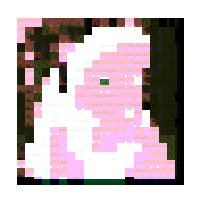
\includegraphics[scale=0.5]{pics/Alice/Nassaualice}}}
    = \vcenter{\hbox{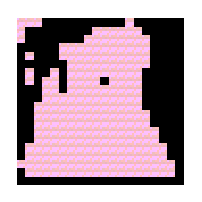
\includegraphics[scale=0.5]{pics/Alice/Nassaualice1}}}
    \oplus \vcenter{\hbox{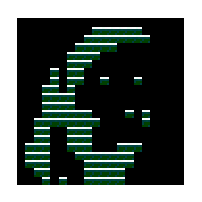
\includegraphics[scale=0.5]{pics/Alice/Nassaualice3}}}
    \oplus \vcenter{\hbox{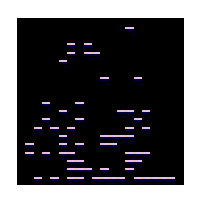
\includegraphics[scale=0.5]{pics/Alice/Nassaualice4}}}
    \oplus \vcenter{\hbox{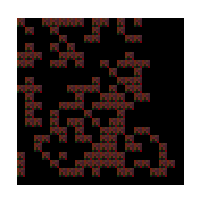
\includegraphics[scale=0.5]{pics/Alice/Nassaualice7}}} & \rotatebox[origin=c]{90}{\footnotesize(\textsc{Nassau})}\\
    %---------------- MDL4bmf
    &\approx
    \vcenter{\hbox{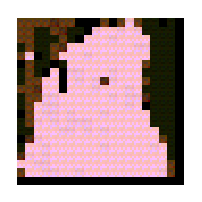
\includegraphics[scale=0.5]{pics/Alice/Mdl4bmfalice}}}
    = \vcenter{\hbox{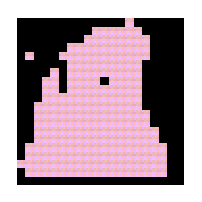
\includegraphics[scale=0.5]{pics/Alice/Mdl4bmfalice1}}}
    \oplus \vcenter{\hbox{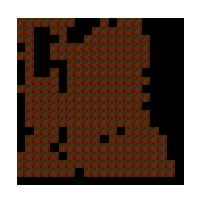
\includegraphics[scale=0.5]{pics/Alice/Mdl4bmfalice3}}}
    & \rotatebox[origin=c]{90}{\footnotesize (\textsc{Mdl4bmf}) }\\
    %---------------- Panda
    &\approx
    \vcenter{\hbox{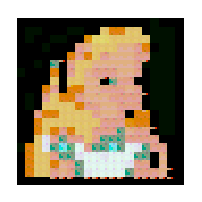
\includegraphics[scale=0.5]{pics/Alice/Pandaalice}}}
    = \vcenter{\hbox{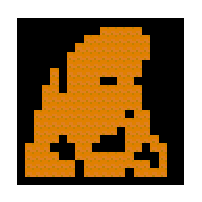
\includegraphics[scale=0.5]{pics/Alice/Pandaalice1}}}
    \oplus \vcenter{\hbox{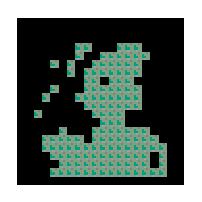
\includegraphics[scale=0.5]{pics/Alice/Pandaalice2}}}
    \oplus \vcenter{\hbox{
\includegraphics[scale=0.5]{pics/Alice/Pandaalice3}}}
    \oplus \vcenter{\hbox{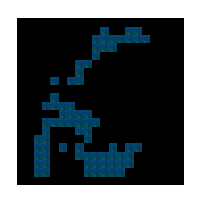
\includegraphics[scale=0.5]{pics/Alice/Pandaalice4}}}&\rotatebox[origin=c]{90}{ \footnotesize(\textsc{Panda+})}\\
    %-----------------Panpal---------------
     &\approx
     \vcenter{\hbox{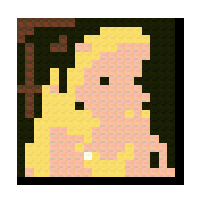
\includegraphics[scale=0.5]{pics/Alice/PanPalAlice}}}
    = \vcenter{\hbox{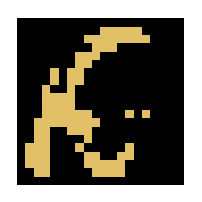
\includegraphics[scale=0.5]{pics/Alice/PanPalAlice1}}}
    \oplus \vcenter{\hbox{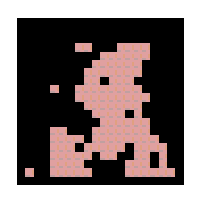
\includegraphics[scale=0.5]{pics/Alice/PanPalAlice4}}}
    \oplus \vcenter{\hbox{
\includegraphics[scale=0.5]{pics/Alice/PanPalAlice5}}}
    &\rotatebox[origin=c]{90}{\footnotesize(\textsc{Panpal}) }\\
     %-----------------Primp---------------
     &\approx
     \vcenter{\hbox{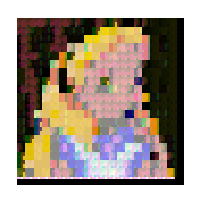
\includegraphics[scale=0.5]{pics/Alice/PrimpAlice}}}
    = \vcenter{\hbox{\includegraphics[scale=0.5]{pics/Alice/PrimpAlice1}}}
    \oplus \vcenter{\hbox{\includegraphics[scale=0.5]{pics/Alice/PrimpAlice3}}}
    \oplus \vcenter{\hbox{\includegraphics[scale=0.5]{pics/Alice/PrimpAlice4}}}
    \oplus \vcenter{\hbox{\includegraphics[scale=0.5]{pics/Alice/PrimpAlice6}}}& \rotatebox[origin=c]{90}{\footnotesize (\textsc{Primp}) }
  \end{align*}
  \caption{Reconstructions of the alice image and visualizations of the top-4 outer products. Best viewed in color.\label{fig:alice}}
\end{figure}

The original Alice image, as well as reconstructions $\theta(XY)$ and the top-4 tiles generated by \textsc{Nassau}, \textsc{Mdl4bmf}, \textsc{Panda+}, \textsc{Panpal} and \textsc{Primp}, are depicted in Figure~\ref{fig:alice}. 
Clearly, only \textsc{Panda+} and \textsc{Primp} select patterns, i.e., blocks of pixels which provide a reasonable reconstruction of the original image. \textsc{Panpal}'s tendency to underestimate the rank (choosing only three tiles) becomes apparent here again.
Regarding the figured structures, \textsc{Panda+}, \textsc{Panpal} and \textsc{Primp} discover a hair-related substructure, where the one found by \textsc{Primp} has the most distinctive contours, and \textsc{Panda+}, \textsc{Panpal} and \textsc{Primp} identify a face-related structure. The reconstructions and factors found by \textsc{Nassau} and \textsc{Mdl4bmf} are not easy to interpret without knowledge of the original image. 

\begin{figure}
  \begin{align*}
    &\vcenter{\hbox{\includegraphics[scale =0.2]{pics/SpaceInv/spaceInv}}}\\
    %---------------- MDL4bmf
    &\quad\approx
    \vcenter{\hbox{\includegraphics[scale =0.2]{pics/SpaceInv/NassauspaceInv}}}
    = \vcenter{\hbox{\includegraphics[scale =0.2]{pics/SpaceInv/NassauspaceInv1}}}
    \oplus \vcenter{\hbox{\includegraphics[scale =0.2]{pics/SpaceInv/NassauspaceInv2}}}
    \oplus \vcenter{\hbox{\includegraphics[scale =0.2]{pics/SpaceInv/NassauspaceInv8}}}
    \oplus \vcenter{\hbox{\includegraphics[scale =0.2]{pics/SpaceInv/NassauspaceInv11}}} & \rotatebox[origin=c]{90}{\footnotesize(\textsc{Nassau})}\\
    %---------------- MDL4bmf
    &\quad\approx
    \vcenter{\hbox{\includegraphics[scale =0.2]{pics/SpaceInv/Mdl4bmfspaceInv}}}
    = \vcenter{\hbox{\includegraphics[scale =0.2]{pics/SpaceInv/Mdl4bmfspaceInv1}}}
    \oplus \vcenter{\hbox{\includegraphics[scale =0.2]{pics/SpaceInv/Mdl4bmfspaceInv2}}}
    \oplus \vcenter{\hbox{\includegraphics[scale =0.2]{pics/SpaceInv/Mdl4bmfspaceInv3}}}
    \oplus \vcenter{\hbox{\includegraphics[scale =0.2]{pics/SpaceInv/Mdl4bmfspaceInv4}}} & \rotatebox[origin=c]{90}{\footnotesize (\textsc{Mdl4bmf}) }\\
    %---------------- Panda
    &\quad\approx
    \vcenter{\hbox{\includegraphics[scale =0.2]{pics/SpaceInv/PandaspaceInv}}}
    = \vcenter{\hbox{\includegraphics[scale =0.2]{pics/SpaceInv/PandaspaceInv1}}}
    \oplus \vcenter{\hbox{\includegraphics[scale =0.2]{pics/SpaceInv/PandaspaceInv2}}}
    \oplus \vcenter{\hbox{\includegraphics[scale =0.2]{pics/SpaceInv/PandaspaceInv3}}}
    \oplus \vcenter{\hbox{\includegraphics[scale =0.2]{pics/SpaceInv/PandaspaceInv4}}}&\rotatebox[origin=c]{90}{ \footnotesize(\textsc{Panda+})}\\
    %-----------------Panpal---------------
     &\quad\approx
     \vcenter{\hbox{\includegraphics[scale =0.2]{pics/SpaceInv/PanPalSpaceInv}}}
    = \vcenter{\hbox{\includegraphics[scale =0.2]{pics/SpaceInv/PanPalSpaceInv1}}}
    \oplus \vcenter{\hbox{\includegraphics[scale =0.2]{pics/SpaceInv/PanPalSpaceInv2}}}&\rotatebox[origin=c]{90}{\footnotesize(\textsc{Panpal}) }\\
     %-----------------Primp---------------
     &\quad\approx
     \vcenter{\hbox{\includegraphics[scale =0.2]{pics/SpaceInv/PrimpSpaceInv}}}
    = \vcenter{\hbox{\includegraphics[scale =0.2]{pics/SpaceInv/PrimpSpaceInv1}}}
    \oplus \vcenter{\hbox{\includegraphics[scale =0.2]{pics/SpaceInv/PrimpSpaceInv2}}}
    \oplus \vcenter{\hbox{\includegraphics[scale =0.2]{pics/SpaceInv/PrimpSpaceInv3}}}& \rotatebox[origin=c]{90}{\footnotesize (\textsc{Primp}) }
  \end{align*}
  \caption{Reconstructions of the Space Invaders image and visualizations of the top-4 outer products. Best viewed in color.\label{fig:spaceInv}}
\end{figure}
Reconstruction results and top-4 patterns of the Space Invaders image are shown in Figure~\ref{fig:spaceInv}. All methods reconstruct at least the shape of the aliens. In terms of color, however, the results diverge. \textsc{Panda+} and \textsc{Nassau} interpret all colors as negative noise effects on the color white; white has a binary representation of $24$ ones. \textsc{Panpal} recovers the yellow color correctly and it extracts the full blue channel from the image---an identical pattern is also detected by \textsc{Primp}. \textsc{Primp} and \textsc{Mdl4bmf} reconstruct all three colors of the original image, yet the reconstruction of \textsc{Mdl4bmf} exhibits injections of white blocks. Hence, only \textsc{Primp} is capable to reconstruct the color information correctly. 

Having a look at derived tiles, the greedy processes of \textsc{Panda+} and \textsc{Nassau} become particularly visible; \textsc{Panda+} and \textsc{Nassau} overload the first factor with all the shape information. The remaining factors reduce the quantitative reconstruction error, but have no deeper interpretation. \textsc{Mdl4bmf} tries to model one type of aliens by each tile. Although this would result in a reasonable description of the image, the actual extraction of tiles suffers from the greedy implementation. We can see that, e.g., the first tile captures information about the yellow aliens as well as strayed parts of other aliens. This unfortunate allocation of tiles results in the injection of white blocks in the reconstruction image.  \textsc{Panpal} clearly separates yellow and blue aliens but interprets differences from the color blue to purple and to turquoise as noise. Finally, \textsc{Primp} separates by its tiles the three basic color channels which are actually used to mix the colors that appear in the original image. Hence, \textsc{Primp} achieves the factorization rank that corresponds to the natural amount of color concepts in the image, unlike all other competitors.

The results of this qualitive experiment particularly illustrates the benefits of a non-greedy minimization procedure. Even though \textsc{Panpal} is often not able to minimize the costs due to an underestimation of the rank, its categorization into tiles always yields interpretable parts.
%=====================
% Discussion
%=====================
\section{Discussion}
We introduce the minimization of description lengths for the derivation of Boolean matrix factorizations with an automatically determined rank by \textsc{PAL-Tiling}. Requiring that the description length has a smooth relaxed function, which combines the matrix factorization error with a regularizing function, \textsc{PAL-Tiling} minimizes the relaxed objective under convergence guarantees. %A thresholding to binary values according to the actual cost measure enables an automatic determination of the factorization rank.

Aiming at the robust identification of Boolean matrix factorizations in presence of various noise distributions, we consider two description lengths in this framework which defines two factorization algorithms. The first algorithm uses a simple $\ell 1$-norm regularization on the factor matrices and is called \textsc{Panpal}. The second minimizes the MDL-description length of the encoding by code tables as known from \textsc{Krimp} \citep{siebes2006item}. Foregoing the heuristics in computing the usage of codes, we extend the application of this encoding from pattern mining to Boolean matrix factorization and derive an upper bound which induces the relaxed objective. We refer to this instance of \textsc{PAL-Tiling} as \textsc{Primp}.

Our experiments on synthetically generated datasets show  that the quality of competing algorithms \textsc{Panda+}, \textsc{Mdl4bmf} and \textsc{Nassau} is sensitive towards multiple data generation parameters. The first of the two newly introduced algorithms, \textsc{Panpal}, regularly underestimates the true factorization rank. We have seen that this property can be beneficial in settings with large, overlapping tiles which induce dense datasets (cf.\@ Figure\@ \ref{fig:density}). In all other settings, the second algorithm \textsc{Primp} is able to detect the underlying structure, regardless of the considered distribution of noise or variations the factorization rank (cf.\@ Figures \ref{fig:noise810}-\ref{fig:rank}). 

A comparison of cost measures, as provided by the description lengths, on real-world datasets show that \textsc{Primp} also most often achieves lowest costs (cf.\@ Table\@ \ref{tbl:realWorldCosts}). With experiments based on images, we visualize the derived tiles under  presence of ambiguous factorization structures and special noise distributions (cf.\@ Figures \ref{fig:alice} and \ref{fig:spaceInv}). The quality of the reconstruction by established algorithms varies considerably between both images. On the contrary, \textsc{Panpal} and \textsc{Primp} provide solid representations of the original images. The extracted factors reveal a parts-based decomposition of the data (as known from non-negative matrix factorizations), which allows for interpretation of the results. In the Space Invaders image (cf.\@ Figure\@ \ref{fig:spaceInv}), \textsc{Panpal} partitions the space invaders into those with a non-zero blue component in their color (rank-1 factorization 2) and those with a zero blue component in their color (rank-1 factorization 1). On the other hand, \textsc{Primp} divides the space invaders by the primary colors they contain (repeating each space invader exactly twice, hence finding structure in the data too, albeit a different structure from the one found by \textsc{Panpal}). From the Alice image (cf.\@ Figure~\ref{fig:alice}) particularly \textsc{Primp} manages to extract coherent factors representing the hair (rank-1 factorization 1) and the face (rank-1 factorization 4).

The implementation of the other popular cost measure, the Typed XOR DtM, is not readily realizable in \textsc{PAL-Tiling}. A real-valued relaxation of this description length involves the gamma function, which is not definable and thus, we cannot say whether this description length is a \KL function. Therefore, convergence to a local extremal point of the relaxed Typed XOR DtM function is not guaranteed in PALM. However, other description lengths are possibly worth exploring. For instance, a symmetric regularization of factor matrices appears to be more suitable in the scope of BMF, opposed to the asymmetric regularization implemented by \textsc{Primp}. The formulation of a description length which equally penalizes the model complexity in an encoding by code tables could simplify the implementation effort of \textsc{Primp} while maintaining the ability to suitably select the rank.
%Furthermore, the application of other penalizing functions $\phi$ is possible if the corresponding $\prox$-operator can be derived. 
%An analysis of the synergy between the penalizing function, the cost-measure and the thereby derived Boolean Matrix Factorization has the potential to show how the structure from arbitrary binary datasets can be robustly identified.
%\chapter{BMF Rank Selection by the False Discovery Rate}
\chaptermark{BMF Rank Selection by FDR}\label{chap:RankFDR}

Often enough in explorative data mining, the user is left alone with the result; a bunch of groupings which supposedly expresses the underlying relations in the dataset. The absence of quality guarantees is an eyesore for the painstaking data miner.
Whenever data is collected from an imperfect (noisy) channel---arising from tainted or inaccurate measurements, or transmission errors---the method of choice might be fooled by the noise, resulting in phantom patterns which actually don't exist in the data. Thus, the investigation of \emph{trustworthiness} of data mining techniques is important in practice. While some approaches for the supervised setting exist, e.g., significant pattern mining~\citep{llinares2015fast}, statistical emerging pattern mining~(\cite{komiyama2017statistical} and references therein), insights for the unsupervised case are still missing. 

In the scope of Boolean matrix factorization, if some of the modeled tiles emerge from noise, false discoveries happen and the algorithm overfits.
We prove two bounds on the probability that a found tile is constituted of random Bernoulli-distributed noise. Both allow us to exploit specific properties of a tile, resulting in different strengths for different types of input data.
The bounds require an additional input from the user: an estimate to the positive noise level $p_+$. While this might seem to be a prohibitive burden, our experimental results show that a rough estimate suffices---the user should merely know if her data is pretty noisy or not so much.

The state-of-the-art BMF techniques filter the structure from the noise and estimate the rank by employing rather complicated regularization terms originating from the description lengths when encoding the data. The belief in the correctness of these algorithms is based on empirical evaluations, inter alia, experiments with synthetically added Bernoulli-distributed noise. 
Under this noise assumption, we employ our bounds to devise a new, theoretically well-founded, rank estimation strategy. Since our technique may be used as a plug-in replacement for existing heuristics, our findings improve a whole class of BMF algorithms.
%-------------------------------
% Main Contributions
%--------------------------------
Our main contributions are:
\begin{itemize}
\item the first provision of bounds on the probability that a tile with specified properties is generated from random noise;
\item the validation of required properties for factorizations which minimize the approximation error, showing that both bounds are non-trivial;
\item the exemplification of algorithmic use of the bounds for automatic rank selection and the empirical evaluation on synthetic and real-world datasets---a step towards trustworthy data mining. 
\end{itemize}
%=====================================
% Bounding False Discoveries
%=====================================
\section{False Discoveries in Boolean Matrix Factorization}\label{sec:TP:boundingFDR}
We now explicitly distinguish between the noise flipping a zero to a one (positive noise) and the one flipping a one to a zero (negative noise). The Boolean decomposition distinguishing between these noise effects is given as follows:
\begin{align}\label{eq:BMF0}
D=(Y^*\odot {X^*}^\top \oplus N_+) \circ (\thickbar{Y^*\odot {X^*}^\top} \oplus \thickbar{N_-}).
\end{align}
The factor matrices $X^*\in\{0,1\}^{n\times r}$ and $Y^*\in\{0,1\}^{m\times r}$ denote the \emph{true} model and $N_+,N_-\in\{0,1\}^{m\times n}$ are the binary positive and negative noise matrices. 

The first step towards trustworthy pattern mining is a measure of trustworthiness. 
The False Discovery Rate (FDR)~\citep{benjamini1995controlling} is a simple yet powerful way to express the probability that something goes wrong.
%-------- Def FDR ---------
\begin{definition}[FDR]
Let $\mathcal{H}$ be a finite set of null hypotheses from which $r$ are rejected. Let $v$ denote the number of erroneously rejected null hypotheses. We say that \emph{the FDR is controlled at level $q$} if
\begin{align*}
\mathbb{E}\left(\frac{v}{r}\right)\leq q.
\end{align*}
\end{definition}
In our setting, a null hypothesis states that the intersections of columns and rows indicated by a tile $yx^\top$ do not reflect underlying relations. In other words, the hypothesis $H_s^0$ is true when there is no overlap between the underlying model $Y^*{X^*}^\top$ and the outer product of the $s$-th tile $Y_{\cdot s}X_{\cdot s}^\top$. This definition of a null hypothesis might seem too restrictive for some applications. Therefore, we discuss possible relaxations of this requirement in Section~\ref{sec:TP:rejectNullHyp}. 
Bearing this in mind, we see that a BMF of rank $r$ corresponds to a joint rejection of $r$ null hypotheses $\{H_1^0,H_2^0,\dots,H_r^0\}$. 
Thus, if the correct rank is $r^*$, any rank $r>r^*$ factorization is likely to state some erroneous rejections of null hypotheses, a.k.a. false discoveries. 

Now, given factor matrices $X\in \{0,1\}^{n\times r}$ and $Y\in\{0,1\}^{m\times r}$, we define a random variable $Z_s$ with domain $\{0,1\}$, which takes the value $1$ if and only if the null hypothesis $H_s^0$ is not to be rejected, i.e., the outer product $Y_{\cdot s}X_{\cdot s}^\top $ covers only (or mostly -- depending on the definition) noise. The FDR of a BMF is therefore computed via
\begin{align}
\mathbb{E}\left(\frac{v}{r}\right) = \frac{1}{r}\sum_{s=1}^rP(Z_s=1)\;.\label{eq:FDRZ}
\end{align}
%--------------------------------------
% Tiles in Bernoulli Matrices
%--------------------------------------
\subsection{Tiles in Bernoulli Matrices}
We aim at assessing the probability $P(Z_s=1)$. Therefore, we need to employ an independence assumption on the noise. 
%-------- Def Bernoulli Matrix --------
\begin{definition}[Bernoulli matrix]
Let $B$ be an $m\times n$ binary matrix. If the entries of $B$ are independent Bernoulli variables, which take the value $1$ with probability $p$ and zero otherwise, i.e., 
\[P(B_{ji}=1)=p,\ P(B_{ji}=0)=1-p\;,\]
then $B$ is a \emph{Bernoulli $(p)$ matrix}.
\end{definition}
In what follows, we assume that the positive noise matrix $N_+$ is a Bernoulli matrix. If a tile $Y_{\cdot s}X_{\cdot s}^\top$ does not approximate the model $Y^*{X^*}^\top$ then it has to have some overlap with the positive noise matrix, otherwise the tile wouldn't contribute to minimizing the approximation error to the data. The \emph{overlap} is computed as the sum of common $1$ entries
\[|Y_{\cdot s}X_{\cdot s}^\top\circ N_+|=\langle Y_{\cdot s}X_{\cdot s}^\top,N_+\rangle=\tr(X_{\cdot s}Y_{\cdot s}^\top N_+)=Y_{\cdot s}^\top N_+X_{\cdot s}\;.\]
This quantity is used to determine the density of a tile in the positive noise matrix.
%----- Def dense on -------
\begin{definition}[$\delta$-dense]
Let $A$ be an $m\times n$ binary matrix and $\delta\in[0,1]$. We say a tile or binary outer product $yx^\top$ is \emph{$\delta$-dense in $A$}  if
\[y^\top A x \geq \delta |x||y|\;.\]
\end{definition}
Since a Boolean matrix product, approximating the data matrix well, covers a high proportion of ones in $D$, the tiles returned by a Boolean factorization are expected to be dense in $D$. We will discuss in the following section how dense a tile has to be in a matrix in order to approximate it well. The following theorem explores the probability with which a $\delta$-dense tile of given minimal size exists in a Bernoulli matrix. This gives us an upper bound on the probability $P(Z_s=1)$ from Eq.~\eqref{eq:FDRZ}, which in turn allows us to bound the FDR.
%------ THEOREM Density Bound ------
\begin{theorem}\label{thm:densProb}
Suppose $B$ is an $m\times n$ Bernoulli $(p)$ matrix, $\delta\in[0,1]$, $1\leq a\leq n$, and $1\leq b\leq m$. 
The probability that a $\delta$-dense tile of size $|x|\geq a$ and $|y|\geq b$ exists is no larger than
\begin{align}\label{eq:densBound}
\binom{n}{a}\binom{m}{b}\exp(-2ab(\delta-p)^2)\;.
\end{align}
\end{theorem}
\begin{proof}
If a $\delta$-dense tile $(x,y)$ exists in $B$, having the size  $(|x|,|y|)\geq (a,b)$, then we can construct a $\delta$-dense sub-tile of exact size $(a,b)$. This follows by induction from the observation that removing the sparsest column/row in $B\circ yx^\top$ from the tile does not decrease the density. Thus, the probability that a $\delta$-dense tile of size at least $(a,b)$ exists is no larger than the probability that a tile of size $(a,b)$ exists.  

Now, let $(x,y)$ be such a tile with $|x|= a$ and $|y|= b$. The probability that $(x,y)$ is $\delta$-dense in $B$ is equal to
\begin{align*}
P\left(\frac{y^\top Bx}{|x||y|}\geq \delta\right)
&=P\left(\left(\frac{1}{ab}\sum_{i,j}x_iy_jB_{ji}\right)-p\geq \delta-p\right)\\
&\leq \exp(-2ab(\delta-p)^2),
\end{align*}
where the inequality follows from Hoeffding's inequality.
An application of the union bound over all possible combinations to place $a$ ones in $x$ and $b$ ones in $y$ yields the statement of the theorem.
\end{proof}
The proof of Theorem~\ref{thm:densProb} indicates that the tightness of the bound in Eq.~\eqref{eq:densBound} might suffer from the extensive use of the union bound. This originates from the numerous possibilities to select a set of columns and rows of given cardinality. If we expect that rows and columns which are selected by a tile have proportionately many ones in common, we bypass the requirement to take all possible column and row selections into account. To this end, given an $m\times n$ matrix $B$, we assess the value of the function 
\[
\eta(B)= \max_{1\leq i\neq k\leq n} \langle B_{\cdot i},B_{\cdot k}\rangle\;.
\] 
%----- THEOREM coherence bound ---
\begin{theorem}\label{thm:cohBound}
Let $B$ be an $m\times n$ Bernoulli $(p)$ matrix and let $\tau>p^2$. The function value of $\eta$ satisfies
$
\eta\left(({1}/\sqrt{m})B\right) \geq \tau
$
with probability no larger than
\begin{align}\label{eq:cohBound}  
\frac{n(n-1)}{2}\exp\left( -\frac{3}{2}m\frac{(\tau-p^2)^2}{2p^2+\tau}\right). 
\end{align}
\end{theorem}
%
\begin{proof}
Let $B$ be as described above and $1\leq i\neq k\leq n$. The variance of the random variable $B_{ji}B_{jk}$ is
\[\mathbb{E}\left[\left(B_{ji}B_{jk}-p^2\right)^2\right]=p^2(1-p^2)\;.\]
Since the variables $B_{ji}B_{jk}$ are independent for $j\in\{1,\ldots,m\}$, the Bernstein inequality yields 
\begin{align*}
&P(\langle B_{\cdot i},B_{\cdot k}\rangle\geq m\tau) 
=P\left(\sum_j (B_{j i}B_{j k}-p^2)\geq m\tau-mp^2\right)\\
&\leq \exp\left(-1/2 \frac{(m\tau-mp^2)^2}{mp^2(1-p^2)+1/3(m\tau-mp^2)}\right)
\leq \exp\left(-1/2 \frac{m(\tau-p^2)^2}{2/3p^2+1/3\tau}\right)
\end{align*}
%\begin{align*}
%P(\langle B_{\cdot i},B_{\cdot k}\rangle\geq m\mu) & \leq \exp\left( -\frac{3}{2}m\frac{(\mu-p^2)^2}{2p^2+\mu}\right)\;,
%\end{align*}
where we made use of the relations $\mathbb{E}[B_{ji}B_{jk}]=p^2$ and $1-p^2\leq 1$.
The union bound over all possible pairs of distinct rows ($i\neq k$) yields the final result.
\end{proof}

If the columns of matrix $B$ are normalized, then the function $\eta(B)$ returns the \emph{coherence} of $B$. The coherence measures how close the column vectors are to an orthogonal system, an extensively studied property in the field of compressed sensing~\citep{foucart2013mathematical}. If all columns of a matrix are orthogonal to each other, then the coherence is zero. The bound in Eq.~\eqref{eq:cohBound} also implies a bound on the coherence of the matrix $B$. Thus, we refer to Bound~\eqref{eq:cohBound} as the \emph{coherence bound} and to Bound~\eqref{eq:densBound} as the \emph{density bound}. For any given tile, we can now derive two upper bounds on the quantity $P(Z_s=1)$ from Eq.~\eqref{eq:FDRZ}, and thus control the FDR.
%-----------------------------------------------------
% Rejecting the Rejection of Null Hypotheses
%-----------------------------------------------------
\subsection{Rejecting the Rejection of Null Hypotheses}\label{sec:TP:rejectNullHyp}
How does the density and the coherence bound now help assessing the  probability $P(Z_s=1)$ from Eq.~\eqref{eq:FDRZ}? Let us reconsider the universal formulation of a null hypothesis, which poses that a tile does not reflect actual relations given by the \emph{true} model $Y^*{X^*}^\top$. First, we relax this definition by counting those tiles which cover only a fraction of the \emph{true} model among the false discoveries as well. Given factor matrices $X$ and $Y$ and and a fraction parameter $t\in[0,1]$, we define the null hypothesis $H_s^0(\alpha)$ to be true if the overlap between the $s$-th tile and the model is smaller than 
\begin{align}\label{eq:nullHyp}
P(Z_s=1)\Leftrightarrow \frac{|Y_{\cdot s}X_{\cdot s}^\top\circ Y^*{X^*}^\top|}{|Y_{\cdot s}X_{\cdot s}^\top|}\leq \alpha.
\end{align}
%----- COROLLARY dens bound ----------
\begin{corollary}\label{thm:densZ}
Let $D$ be composed as denoted in Eq.~\eqref{eq:BMF0} and let $N_+$ be a Bernoulli $(p_+)$. Given $X\in\{0,1\}^{n\times r}$ and $Y\in\{0,1\}^{m\times r}$ with 
\[Y_{\cdot s}^\top DX_{\cdot s}\geq \delta_s|Y_{\cdot s}||X_{\cdot s}|,\] 
then for $\rho = \max\{\delta_s-\alpha-p,0\}$, the probability that  the null hypothesis $H_s^0(\alpha)$ is true and thus not to be rejected is bounded by
\begin{align*}
P(Z_s=1)= P\left(\frac{|Y_{\cdot s}X_{\cdot s}^\top\circ Y^*{X^*}^\top|}{|Y_{\cdot s}X_{\cdot s}^\top|}\leq \alpha\right)\leq \binom{n}{|X_{\cdot s}|}\binom{m}{|Y_{\cdot s}|}\exp(-2|X_{\cdot s}||Y_{\cdot s}|\rho^2)
\end{align*}
\end{corollary}
\begin{proof}
We apply the triangle inequality to the decomposition of $D$ given by Eq.~\eqref{eq:BMF0}, yielding
\[|Y_{\cdot s}^\top DX_{\cdot s}|\leq |Y_{\cdot s}X_{\cdot s}^\top\circ Y^*{X^*}^\top|+|Y_{\cdot s}X_{\cdot s}^\top \circ N_+|.\]
Dividing by $|Y_{\cdot s}||X_{\cdot s}|$ and applying Eq.~\eqref{eq:nullHyp} yields that $(X_{\cdot s},Y_{\cdot s})$ is $\delta_s-t$-dense in $N_+$.
%\[\frac{|Y_{\cdot s}X_{\cdot s}^\top \circ N_+|}{|Y_{\cdot s}||X_{\cdot s}|}\geq \delta_s-t.\]
The probability for this event is bounded by Theorem~\ref{thm:densProb}.
\end{proof}
Similar considerations lead to a false discovery bound based on coherence. In this setting, we define the null hypothesis $H_s^0(\beta)$ for $\beta\in\mathbb{N}$ to hold if 
\begin{align}\label{eq:nullHypCoh}
Z_s=1 \Leftrightarrow \eta(Y_{\cdot s}X_{\cdot s}\circ Y^*{X^*}^\top)\leq \beta.
\end{align}
This restriction affects the tilewise overlap between the underlying and the computed model more than the definition based on density does. As such, Eq.~\eqref{eq:nullHypCoh} implies that each column of the outer product $Y_{\cdot s}{X_{\cdot s}}^\top$ covers at most $\beta$ rows of each tile $Y^*_{\cdot t}{X^*_{\cdot t}}^\top$ of the underlying model. The probability of a false discovery according to this definition of a null hypothesis is bounded by the following corollary. 
%----------- COROLLARY coherence bound -----
\begin{corollary}\label{thm:cohZ}
Let $D$ be composed as denoted in Eq.~\eqref{eq:BMF0} and let $N_+$ be a Bernoulli $(p_+)$ matrix. Given $X\in\{0,1\}^{n\times r}$ and $Y\in\{0,1\}^{m\times r}$ such that 
\[\eta(Y_{\cdot s}X_{\cdot s}^\top \circ D)\geq \tau_s m,\] 
then for $\rho = \max\{\tau_s-\nicefrac{\beta}{m},p^2\}$, the probability that the null hypothesis $H_s^0(\beta)$ holds as defined in Eq.~\eqref{eq:nullHypCoh} is bounded by
\begin{align*}
P(Z_s=1)=P\left(\eta(Y_{\cdot s}X_{\cdot s}\circ Y^*{X^*}^\top)\leq \beta\right)\leq \frac{n(n-1)}{2}\exp\left(-\frac{3}{2}m\frac{(\rho-p^2)^2}{2p^2+\rho}\right)
\end{align*}
\end{corollary}
\begin{proof} 
From the composition of $D$ as denoted in Eq.~\eqref{eq:BMF0} and the definition of $\eta$, computing a maximum, follows that 
\[\eta(Y_{\cdot s}X_{\cdot s}^\top \circ D)\leq \eta(Y_{\cdot s}X_{\cdot s}^\top \circ Y^*_{\cdot s}{X^*_{\cdot s}}^\top)+\eta(Y_{\cdot s}X_{\cdot s}^\top \circ N_+).\]
Applying Eq.~\eqref{eq:nullHypCoh} and $\eta(Y_{\cdot s}X_{\cdot s}^\top \circ D)\geq \mu m$ yields
$\eta(N_+)\geq \mu m-t$.
The probability that this inequality holds is bounded by Theorem~\ref{thm:cohBound}.
\end{proof}
We assume from now on that $\alpha=\beta=0$, by what both definitions of the null hypothesis concur. The following results are though easily adapted to a parametrized definition of the null hypothesis.  
%=====================================
% Theoretical Comparison of the Proposed Bounds
%=====================================
\section{Theoretical Comparison of Proposed Bounds}\label{sec:theoryCompare}
The bounds from the previous section supposedly enable a theoretically well-founded approach to select the rank for a Boolean factorization. Given any factorization, the proposed bounds help to toss all tiles which may just as well have arisen from noise.
However, the tightness of the bounds is the linchpin of the applicability of this scheme. 
%In return, we do not need to worry about a suitable regularization term which penalizes the formation of superfluous tiles. 
Since we do not require a penalization term of the model complexity to determine the correct rank in the FDR controlled scenario, we can choose the most simple objective function: the residual sum of squares as defined in problem~\eqref{eq:BoolMF}.
The minimization of the residual sum of absolute values $F_{RSS}(X,Y)$ is not only simple to implement, but this function is also simple enough to let us derive characteristics of its optima with regard to coherence and minimum density of tiles. This enables a theoretic characterization of those tiles which would be tossed by the bounds. Moreover, this contributes to a fundamental understanding of the nature of tiles in a minimizing factorization. Assuming the data is composed as stated in Eq.~\eqref{eq:BMF0}, we explore the circumstances which have to be met such that a tile in the noise matrix contributes to minimizing $F_{RSS}(X,Y)$.
%------- lemma density overlap -----------
\begin{lemma}\label{thm:minDensOverlap}
Let $X$ and $Y$ be $n\times r$ and $m\times r$ binary matrices and let $s\in\{1,\ldots,r\}$. If $(X,Y)$ is a solution of \eqref{eq:BoolMF}, then the density of tile $(x,y)=(X_{\cdot s},Y_{\cdot s})$ is lower-bounded on the area which is  not covered by any other tile, i.e.,
\begin{align}\label{eq:densOverlap}
\frac{y^\top (D\circ \thickbar{M})x}{y^\top \thickbar{M}x}
\geq \frac{1}{2},
\end{align}
where $M =\bigoplus_{t\neq s}Y_{\cdot t}X_{\cdot t}^\top$ denotes the Boolean product of the factor matrices, excluding the $s$-th tile.
\end{lemma}
%
\begin{proof}
Let $X,\ Y$, $M$ and $(x,y)$ be as described above. The Boolean product of $X$ and $Y$ is written in dependence of $M$ as  
\begin{equation*}
Y\odot X^\top= Y_{\cdot 1}X_{\cdot 1}^\top\oplus\ldots\oplus Y_{\cdot r}X_{\cdot r}^\top = M + yx^\top \circ \thickbar{M}.
\end{equation*}
The approximation error of a Boolean product is the sum of uncovered ones and covered zeros in the data: 
\begin{align*}
|D-Y\odot X^\top | 
&=\langle D-\mathbf{1}+\mathbf{1}-Y\odot X^\top,D-Y\odot X^\top\rangle\\
&=\ \langle D,\thickbar{Y\odot X^\top }\rangle +\langle\thickbar{D},Y\odot X^\top \rangle\\
&=\ \langle D,\thickbar{M+ yx^\top \circ \thickbar{M}}\rangle +\langle\thickbar{D},M+ yx^\top \circ \thickbar{M}\rangle\\
&=\ \langle D,\thickbar{M}\rangle - y^\top (D\circ \thickbar{M})x +\langle\thickbar{D},M\rangle + y^\top (\thickbar{D}\circ \thickbar{M})x\\
&=\ |D-M| - y^\top (D\circ \thickbar{M})x + y^\top (\thickbar{D}\circ \thickbar{M})x.
\end{align*}
Since $(X,Y)$ minimizes $F_{RSS}$, the gap between the function values $|D-M|-F_{RSS}(X,Y)$ is nonnegative. Hence
\begin{equation*}
 y^\top (D\circ \thickbar{M})x - y^\top (\thickbar{D}\circ\thickbar{M})x= 2y^\top (D\circ \thickbar{M})x - y^\top \thickbar{M}x \geq 0.
\end{equation*}
Transforming this inequality yields the final result.
\end{proof}
%
Note that the proof of Lemma~\ref{thm:minDensOverlap} implies, that the density in Eq.~\eqref{eq:densOverlap} has to be larger than one half, if the objective function incorporates a regularization term on the factor matrices. This could be for instance the $\ell1$-norm of the matrices. From Lemma~\ref{thm:minDensOverlap} we now conclude the following property of tiles which reflect a false discovery.  
%---------- corollary density no overlap
\begin{corollary}
Let the matrices $X$ and $Y$ solve \eqref{eq:BoolMF}, and let $s\in\{1,\ldots,r\}$. If the tile $Y_{\cdot s}X_{\cdot s}^\top$ is a false discovery and has no overlap with the remaining tiles, i.e., $\langle Y_{\cdot s}, Y_{\cdot t}\rangle\langle X_{\cdot s}, X_{\cdot t}\rangle=0$ for $s\neq t$, then $Y_{\cdot s}X_{\cdot s}^\top$ is $\nicefrac{1}{2}$-dense in the positive noise matrix $N_+$.
\end{corollary}
%
A similar procedure leads to a bound on the coherence.
%------- lemma coherence >k/2 -----------
\begin{lemma} \label{thm:minCohTile}
Let the matrices $X$ and $Y$ solve \eqref{eq:BoolMF} and let $s\in\{1,\ldots,r\}$. If the outer product $Y_{\cdot s}{X_{\cdot s}}^\top$ is $\delta$-dense in $D$, then
\begin{align}
\eta(D) > \delta|Y_{\cdot s}|\frac{\delta|X_{\cdot s}|-1}{|X_{\cdot s}|-1}\label{eq:minCohTile}
\end{align}
\end{lemma}
%
\begin{proof}
Let $X,Y$ and $s$ be described as above. Denote by $\mathcal{K}=\{i\in\{1,\ldots, n\}\mid X_{is}=1\}$ the set of all items indicated by $X_{\cdot s}$. Since the $\ell1$-norm is bounded for a vector $x$ with $a$ nonzero entries by $|x|\leq\sqrt{a}\|x\|$ and since $Y_{\cdot s}X_{\cdot s}^\top$ is $\delta$-dense, it holds that
\begin{align*}
\|\diag(Y_{\cdot s})DX_{\cdot s}\|^2&\geq \frac{|Y_{\cdot s}^\top DX_{\cdot s}|^2}{|Y_{\cdot s}|}\geq \delta^2|Y_{\cdot s}||X_{\cdot s}|^2.
\end{align*} 
The norm above is equal to
\begin{align*}
\|\diag(Y_{\cdot s})DX_{\cdot s}\|^2& = X_{\cdot s}^\top D^\top\diag(Y_{\cdot s})DX_{\cdot s}\\
&=\sum_{i,k\in\mathcal{K}} D_{\cdot i}^\top \diag(Y_{\cdot s})D_{\cdot k}\\
&= Y_{\cdot s}^\top DX_{\cdot s}+\sum_{i\neq k\in\mathcal{K}}D_{\cdot i}^\top \diag(Y_{\cdot s})D_{\cdot k}.
\end{align*}
Combining both (in)equalities above yields
\begin{align*}
\sum_{i\neq k\in\mathcal{K}}D_{\cdot i}^\top \diag(Y_{\cdot s})D_{\cdot k}& \geq Y_{\cdot s}^\top DX_{\cdot s}\left(\frac{Y_{\cdot s}^\top DX_{\cdot s}}{|Y_{\cdot s}|}-1\right)\\
&\geq \delta|Y_{\cdot s}||X_{\cdot s}|\left(\delta|X_{\cdot s}|-1\right).
\end{align*}
According to the pigeonhole principle, indices $i\neq k$ exist, $i,k\in\mathcal{K}$ such that
\begin{displaymath}
~\qquad\qquad\quad\langle D_{\cdot i}, D_{\cdot k}\rangle
> \delta|Y_{\cdot s}|\frac{\delta|X_{\cdot s}|-1}{|X_{\cdot s}|-1}.
\end{displaymath}
\end{proof}
%
If we assume that a tile $(X_{\cdot s},Y_{\cdot s})$ is a false discovery from an optimal solution $(X,Y)$ of \eqref{eq:BoolMF}, then Bound~\eqref{eq:minCohTile} applies to $N_+$.
%--- picture minimal size of tile ----
\begin{figure}
\centering
%\pgfplotsset{
%trustStyle/.style={ctrust,mark options ={ctrust},mark repeat={4}, ultra thick, error bars/.cd,y dir = both, y explicit},
%densStyle/.style={cdens,dashed,mark options ={cdens},mark repeat={4}, ultra thick, error bars/.cd,y dir = both, y explicit},
%}

\begin{tikzpicture}
    \begin{groupplot}[group style={group size= 2 by 1, vertical sep=0.6cm},
    	height=.33\columnwidth,
    	width=.5\columnwidth,
        axis lines = left,
        scaled ticks=false,tick label style={/pgf/number format/fixed}]
        \nextgroupplot[
        	title={$(n,m)=(1000, 800)$},
        	ylabel={$\frac{|Y_{\cdot s}|}{m}$},
            xlabel={$\frac{|X_{\cdot s}|}{n}$},
            xmin=0,xmax=0.045, ymin=0, ymax=0.25,
            legend columns =-1,
        	legend to name=legendTPMinLForK]
        	\addplot+[densStyle]  plot coordinates {
 (0.002,0.80525)
 (0.004,0.56325)
 (0.006,0.36825)
 (0.008,0.23825)
 (0.01,0.16025) 
 (0.012,0.11425)
 (0.014,0.08725)
 (0.016,0.07025)
 (0.018,0.05925)
 (0.02,0.05125) 
 (0.022,0.04625)
 (0.024,0.04125)
 (0.026,0.03825)
 (0.028,0.03525)
 (0.03,0.03325) 
 (0.032,0.03125)
 (0.034,0.03025)
 (0.036,0.02825)
 (0.038,0.02725)
 (0.04,0.02625) 
 (0.042,0.02525)
 (0.044,0.02525)
 (0.046,0.02425)
 (0.048,0.02325)
 (0.05,0.02325) 
    };
    \addlegendentry{density};
    \addplot+[cohStyle]  plot coordinates {
 (0.002,1)
 (0.004,0.24825)
 (0.006,0.20725)
 (0.008,0.19325)
 (0.01,0.18625) 
 (0.012,0.18225)
 (0.014,0.17925)
 (0.016,0.17725)
 (0.018,0.17625)
 (0.02,0.17425) 
 (0.022,0.17325)
 (0.024,0.17325)
 (0.026,0.17225)
 (0.028,0.17225)
 (0.03,0.17125) 
 (0.032,0.17125)
 (0.034,0.17025)
 (0.036,0.17025)
 (0.038,0.17025)
 (0.04,0.17025) 
 (0.042,0.16925)
 (0.044,0.16925)
 (0.046,0.16925)
 (0.048,0.16925)
 (0.05,0.16925) 
    };\addlegendentry{coherence};
%
	\nextgroupplot[title={$(n,m)=(1600, 500)$},
    	xmin=0,xmax=0.045, ymin=0, ymax=0.25,
    	xlabel={$\frac{|X_{\cdot s}|}{n}$}]
                \addplot+[densStyle]  plot coordinates {
 (0.00125,0.812)
 (0.00325,0.459)
 (0.00525,0.25) 
 (0.00725,0.154)
 (0.00925,0.109)
 (0.01125,0.086)
 (0.01325,0.072)
 (0.01525,0.063)
 (0.01725,0.057)
 (0.01925,0.052)
 (0.02125,0.049)
 (0.02325,0.046)
 (0.02525,0.044)
 (0.02725,0.042)
 (0.02925,0.04) 
 (0.03125,0.039)
 (0.03325,0.037)
 (0.03525,0.036)
 (0.03725,0.035)
 (0.03925,0.034)
 (0.04125,0.034)
 (0.04325,0.033)
 (0.04525,0.032)
 (0.04725,0.032)
 (0.04925,0.031)
    };
            	\addplot+[cohStyle]  plot coordinates {
 (0.00125,1)
 (0.00325,0.284)
 (0.00525,0.25) 
 (0.00725,0.239)
 (0.00925,0.233)
 (0.01125,0.23) 
 (0.01325,0.228)
 (0.01525,0.226)
 (0.01725,0.225)
 (0.01925,0.224)
 (0.02125,0.223)
 (0.02325,0.223)
 (0.02525,0.222)
 (0.02725,0.222)
 (0.02925,0.221)
 (0.03125,0.221)
 (0.03325,0.221)
 (0.03525,0.22) 
 (0.03725,0.22) 
 (0.03925,0.22) 
 (0.04125,0.22) 
 (0.04325,0.22) 
 (0.04525,0.22) 
 (0.04725,0.219)
 (0.04925,0.219)
    };
    \end{groupplot}
\end{tikzpicture}\\

\pgfplotslegendfromname{legendTPMinLForK}

\caption{Minimum relative size $\nicefrac{|Y_{\cdot s}|}{m}$, depending on $\nicefrac{|X_{\cdot s}|}{n}$, for which the $P(Z_s=1)\leq 0.01$, based on density (blue) and coherence (green).}
\label{fig:theory}
\end{figure}

These results enable a theoretic comparison of the bounds based on coherence and density. Figure~\ref{fig:theory} contrasts the two bounds for two settings of dimensions. The plot on the left refers to almost square dimensions $(n,m)=(1000,800)$ and the one on the right to more imbalanced dimensions $(n,m)=(1600,500)$. Let $(X,Y)$ be a solution of $\eqref{eq:BoolMF}$ and assume that the positive noise matrix is a Bernoulli $(p)$ matrix with probability $p=0.1$. We plot the minimum relative size $\nicefrac{|Y_{\cdot s}|}{m}$ against the relative size $\nicefrac{|X_{\cdot s}|}{n}$ such that the probability $P(Z_s=1)\leq 0.01$. The blue curve displays the minimum tile size, assessing the false discovery probability by Corollary~\ref{thm:densZ}, while green refers to Corollary~\ref{thm:cohZ}. Thereby, we assume that the tile is $\nicefrac{1}{2}$-dense in $N_+$ and the value $\eta(N_+)$ is bounded by Inequality~\eqref{eq:minCohTile}. Figure~\ref{fig:theory} indicates that under the given circumstances the coherence provides a more loose bound than the density. The difference between the required sizes is larger, if the dimensions are disproportionate, which suggests that more tiles are rejected as potential false discoveries by the coherence bound, in particular for wide or tall data matrices. Most importantly, the density bound is tight enough to let some of the larger tiles of outer products pass, which are generated according to Algorithm~\ref{alg:MDL:generateBMF}. Applying the default parameters, the relative sizes are in the interval from $0.01$ to $0.1$. We can see that the density bound would accept $0.03\times 0.5$ highly noisy tiles (measured in relative size). The theoretical results of the density bound align with the common sense regarding the minimum size of identifiable tiles.   
%=====================================
% Algorithmic Integration of FDR Control
%=====================================
\section{Algorithmic Integration of FDR Control}\label{sec:TP:algorithmicIntegration}
The false discovery bounds might be applied as a postprocessing step to any Boolean factorization result. Here, we also establish the use of these bounds to directly estimate the rank.
In the rounding procedure at the end of the relaxed optimization in \textsc{PAL-Tiling} (Algorithm~\ref{alg:paltiling}), we can integrate a check of the false discovery bounds via a specification of the function \textsc{Toss}.
 
Since we intend to solve problem~\eqref{eq:BoolMF}, a suitable smooth relaxed objective is the residual sum of squares. Therefore, in this version of the \textsc{PAL-Tiling} algorithm, we employ the vanilla Algorithm Specification~\ref{algSpec:BMF} and the function \textsc{Toss} as provided in Algorithm~\ref{alg:FDR:toss}.
%----- algorithm pseudocode ----
\begin{algorithm}[t]
\caption{The tossing functions for the application of \textsc{PAL-Tiling} implementing the determination of the rank via FDR control.}
\begin{algorithmic}[1]
  %\Function{TrustPal}{$D,\hat{p};\Delta_r=10,q = 0.01$}
   % \State $(X_K,Y_K)\gets (\emptyset, \emptyset)$
   % \For {$r\in\{\Delta_r,2\Delta_r,3\Delta_r,\ldots\}$}
   % \State $(X_0,Y_0) \gets $\Call{IncreaseRank}{$X_K, Y_K,\Delta_r$} %\Comment{Append random columns}
   % \For {$k = 0,1,\ldots$}\label{alg:TP:optStart} \Comment{Select stop criterion}
  %  	\State $\alpha_k^{-1} \gets M_{\nabla_XF}(Y_k)$\label{alg:TP:stepX}
   %     \State $X_{k+1} \gets \prox_{\alpha_k\phi}\left(X_k-\alpha_k\nabla_XF(X_k,Y_k)\right)$\label{alg:proxX}
   %    	\State $\beta_k^{-1} \gets M_{\nabla_YF}(X_{k+1})$\label{alg:TP:stepY}
    %    \State $Y_{k+1} \gets \prox_{\beta_k\phi}\left(Y_k-\beta_k\nabla_YF(X_{k+1},Y_k)\right)$\label{alg:TP:proxY}
    %\EndFor
  %  \State $(X,Y)\gets \Call{RoundFDR}{L,X_k,Y_k,\hat{p},q}$ \label{alg:TP:round}
  %  \If {$\Call{RankGap}{X,Y,r}$}
   % 	\textbf{return} $(X,Y)$
   % \EndIf
   % \EndFor
 % \EndFunction
\Function{TossDens}{x,y,D}
    \State $\rho\gets\max\left\{\frac{yDx}{|y||x|} -\alpha -p_+,0\right\}$
    \State \textbf{Return} $\displaystyle\binom{n}{|x|}\binom{m}{|y|}\exp(-2|x||y|\rho^2)>q$
\EndFunction
\State
\Function{TossCoh}{x,y,D}
    \State $\displaystyle\rho\gets\max\left\{\frac{\eta(Y_{\cdot s}X_{\cdot s}^\top\circ D)-\beta}{m}, p_+^2\right\}$
    \State \textbf{Return}$\displaystyle\frac{n(n-1)}{2}\exp\left(-\frac{3}{2}m\frac{(\rho-p^2)^2}{2p^2+\rho}\right)>q$ 
\EndFunction
\end{algorithmic}
\label{alg:FDR:toss}
\end{algorithm}
We call the resulting algorithm \textsc{TrustPal}, which requires additional to the parameters of \textsc{PAL-Tiling} the estimated noise probability $p_+$, the null hypothesis defining parameters $\alpha$, $\beta$ (default value $0$) and the FDR control level $q$ (default value $0.01$). 
The functions in Algorithm~\ref{alg:FDR:toss} define that a tile is supposed to be tossed if the probability of a false discovery is not bounded above by $q$. That is, if Corollary~\ref{thm:densZ} or \ref{thm:cohZ} does not yield $P(Z_s=1)\leq q$, then the tile $s$ is removed from the factorization. Here multiple combinations of the density and coherence bound are possible. Here, we distinguish between \textsc{TrustPal} employing the density bound, that is function \textsc{TossDens} and \textsc{TrustPal} employing the coherence bound, where we toss tile $s$ when \textsc{TossCoh}$(X_{\cdot s},Y_{\cdot s},D)$ and \textsc{TossCoh}$(Y_{\cdot s},X_{\cdot s},D^\top)$ both return true.
The application to the transposed factorization serves a symmetric test of the coherence bound. 
%This is achieved by checking either the density or the coherence bound for every tile. In the first case, the density $\delta_s$ of every tile in $D$ is computed. If tile $(X_{\cdot s},Y_{\cdot s})$ is a false discovery, then it is $\delta_s$-dense in $N_+$. If Bound~\eqref{eq:densBound} yields that $P(Z_s=1)> q$, then we exclude the tile from the returned binary factorization. In the second case, the function value $\eta(D\circ Y_{\cdot s}X_{\cdot s})$ is computed and the probability $P(Z_s=1)$ is bounded by Eq.~\eqref{eq:cohBound}.
%=============================
% Experiments
%============================
\section{Experiments}\label{sec:TP:experiments}
Our experimental evaluation serves the assessment of provided bounds in practical applications. Although the theoretical properties of minimizing factorizations yield satisfactory bounds on the size of a tile (cf.\@ Figure~\ref{fig:theory}), in practice no feasible existing algorithm can guarantee to return optimal solutions of Problem~\eqref{eq:BoolMF}. 
In addition, we show that the estimation of the actual noise probability is not critical in practice.

The implementation of \textsc{TrustPal} follows the highly parallel implementation on graphics processing units (GPU) from the framework \textsc{PAL-Tiling}. All experiments are executed on a GPU with 2688 arithmetic cores and 6GiB GDDR5 memory. The source code of \textsc{TrustPal}, together with Julia scripts to generate data and to compare proposed bounds, is provided\footnote{\url{http://sfb876.tu-dortmund.de/trustpal}}.

We compare the two variants of \textsc{TrustPal}, employing the  bounds based on  density or coherence to determine the rank, and the performance of the algorithm \textsc{Primp}. For both bounds, we assume that the null hypothesis with regard to a tile holds if the tile covers only noise. That is, the parameters of the rounding procedure in Algorithm~\ref{alg:FDR:toss} are set to   $\alpha=\beta=0$. We have seen in the experimental evaluation of Section~\ref{sec:MDL:SynthData} that \textsc{PanPal} displays a strong tendency to underestimate the rank, but is able to yield more accurate results than \textsc{Primp} in some particular settings. Whenever that is the case, we display the results for \textsc{PanPal} in the following plots. 
%--------------------------------------------------------
% Experiments for Synthetically Generated Data
%--------------------------------------------------------
\subsection{Experiments on Synthetic Data}
We generate $1600\times 500$ and $1000\times 800$ data matrices according to Algorithm~\ref{alg:MDL:generateBMF}. For every parameter variation, we generate 8 matrices, 4 for each dimension setting $(n,m)\in\{(1000,800),(1600,500)\}$. If not stated otherwise, the default settings $p_+^*=p_-^*=0.1$, $r^*=25$ and $d=0.1$ apply. 
We compare again the computed models against the planted structure by the adaptation of the micro-averaged $\mathsf{F}$-measure, as discussed in Section~\ref{sec:MDL:SynthData}.
%------- Figure Synth Noise ------------
\begin{figure}[t]
\centering
\begin{filecontents}{BMFDR_DENS_n1000m800F.dat}
x y std
0 0.9851000000000001 0.01
5 0.9943000000000002 0.0
10 0.9947000000000001 0.01
15 0.9972 0.0
20 0.9844500000000002 0.01
25 0.8490500000000001 0.08
\end{filecontents}
\begin{filecontents}{BMFDR_DENS_n1000m800R.dat}
x y std
0 23.1 1.25
5 23.8 1.2
10 25.3 1.34
15 24.5 0.83
20 23.1 1.59
25 15.65 3.67
\end{filecontents}
\begin{filecontents}{BMFDR_COH_n1000m800F.dat}
x y std
0 0.9811499999999999 0.01
5 0.9847999999999999 0.01
10 0.978 0.01
15 0.9778499999999999 0.01
20 0.9603999999999999 0.02
25 0.8709 0.07
\end{filecontents}
\begin{filecontents}{BMFDR_COH_n1000m800R.dat}
x y std
0 21.6 1.93
5 22.1 1.77
10 22.25 2.45
15 22.15 1.79
20 21.9 1.89
25 18.0 3.26
\end{filecontents}
\begin{filecontents}{Primp_n1000m800F.dat}
x y std
0 0.9995 0.0
5 0.9974000000000002 0.0
10 0.998 0.0
15 0.9927999999999999 0.01
20 0.9792 0.01
25 0.9243 0.02
\end{filecontents}
\begin{filecontents}{Primp_n1000m800R.dat}
x y std
0 25.3 0.47
5 25.75 0.72
10 27.3 3.1
15 29.1 4.49
20 29.15 5.69
25 29.2 9.33
\end{filecontents}
\begin{filecontents}{BMFDR_DENS_n1600m500F.dat}
x y std
0 0.99415 0.01
5 0.9957500000000001 0.0
10 0.9925499999999998 0.01
15 0.9868 0.01
20 0.9017000000000002 0.13
25 0.49700000000000005 0.16
\end{filecontents}
\begin{filecontents}{BMFDR_DENS_n1600m500R.dat}
x y std
0 23.95 0.89
5 24.15 0.99
10 25.0 1.12
15 23.85 1.04
20 19.3 4.93
25 7.15 2.3
\end{filecontents}
\begin{filecontents}{BMFDR_COH_n1600m500F.dat}
x y std
0 0.9799999999999998 0.01
5 0.9853 0.01
10 0.9775499999999999 0.01
15 0.97545 0.01
20 0.8505 0.16
25 0.54115 0.16
\end{filecontents}
\begin{filecontents}{BMFDR_COH_n1600m500R.dat}
x y std
0 21.9 1.55
5 22.4 1.27
10 22.1 1.33
15 21.7 1.22
20 16.1 5.3
25 7.85 2.35
\end{filecontents}
\begin{filecontents}{Primp_n1600m500F.dat}
x y std
0 0.9990500000000001 0.0
5 0.9996 0.0
10 0.9985999999999999 0.0
15 0.9935999999999998 0.0
20 0.9740000000000002 0.01
25 0.89265 0.06
\end{filecontents}
\begin{filecontents}{Primp_n1600m500R.dat}
x y std
0 25.25 0.72
5 25.5 0.69
10 25.1 0.31
15 24.35 0.75
20 22.2 2.33
25 18.15 3.9
\end{filecontents}

%\pgfplotsset{
%cohStyle/.style={ctrust,mark options ={ctrust},mark repeat={4}, ultra thick, error bars/.cd,y dir = both, y explicit},
%trustStyle/.style={cdens,dashed,mark options ={cdens},mark repeat={4}, ultra thick, error bars/.cd,y dir = both, y explicit},
%primpStyle/.style={cPrimp,dashed,mark=triangle*,mark options ={cPrimp},mark repeat={3}, ultra thick, error bars/.cd,y dir = both, y explicit},
%}

\begin{tikzpicture}
    \begin{groupplot}[group style={group size= 2 by 2, vertical sep=0.6cm},
    	height=.33\columnwidth,
    	width=.5\columnwidth,
        legend columns =-1,
        axis lines = left]
        %
        \nextgroupplot[ylabel={$\mathsf{F}$},
        	title={$(n,m)=(1000,800)$},
        	xmin=0,xmax=25.5, ymin=0.4, ymax=1.1,
        	legend to name=legendTPSynthExpNoise]
        	\addplot+[densStyle]  table[x=x,y=y,y error=std] {BMFDR_DENS_n1000m800F.dat};
            \addlegendentry{\textsc{TrustPal} dens};
        	\addplot+[cohStyle]  table[x=x,y=y,y error=std] {BMFDR_COH_n1000m800F.dat};
            \addlegendentry{\textsc{TrustPal} coh};
            \addplot+[primpStyle]  table[x=x,y=y,y error=std] {Primp_n1000m800F.dat};
            \addlegendentry{\textsc{Primp}};
            %
        \nextgroupplot[title={$(n,m)=(1600,500)$},
        	xmin=0,xmax=25.5, ymin=0.4, ymax=1.1]
                \addplot+[densStyle]  table[x=x,y=y,y error=std] {BMFDR_DENS_n1600m500F.dat};
        	\addplot+[cohStyle]  table[x=x,y=y,y error=std] {BMFDR_COH_n1600m500F.dat};
            \addplot+[primpStyle]  table[x=x,y=y,y error=std] {Primp_n1600m500F.dat};
            %
        \nextgroupplot[xlabel={$p_{\pm}\ [\%]$},
			ylabel={$r$},
			xmax=25.5, xmin=0, ymin=0, ymax=34.2]
                \addplot+[densStyle]  table[x=x,y=y,y error=std] {BMFDR_DENS_n1000m800R.dat};
        	\addplot+[cohStyle]  table[x=x,y=y,y error=std] {BMFDR_COH_n1000m800R.dat};
            \addplot+[primpStyle]  table[x=x,y=y,y error=std] {Primp_n1000m800R.dat};
                %
       \nextgroupplot[xlabel={$p_\pm\ [\%]$},xmin=0,xmax=25.5, ymin=0, ymax=34.2]
                \addplot+[densStyle]  table[x=x,y=y,y error=std] {BMFDR_DENS_n1600m500R.dat};
        	\addplot+[cohStyle]  table[x=x,y=y,y error=std] {BMFDR_COH_n1600m500R.dat};
            \addplot+[primpStyle]  table[x=x,y=y,y error=std] {Primp_n1600m500R.dat};
    \end{groupplot} 
\end{tikzpicture}\\

\pgfplotslegendfromname{legendTPSynthExpNoise}

\caption{Variation of uniform noise for $1600\times 500$- and $1000\times 800$-dimensional data. Comparison of $\mathsf{F}$-measures (the higher the better) and the estimated rank of the calculated Boolean factorization (the closer to 25 the better) for varying levels of noise indicated on the x-axis.}
\label{fig:TP:noise}
\end{figure}

Figure~\ref{fig:TP:noise} displays the performance of the density and coherence approach of \textsc{TrustPal} with \textsc{Primp}. The noise probability varies between $p_\pm^*\in\{0,0.05,\ldots,0.25\}$. While the plots on the left show aggregated results over 20 almost square $1000\times 800$ matrices, the plots on the right refer to 20 more imbalanced datasets with dimension $1600\times 500$. The input parameter of \textsc{TrustPal}, the estimated noise probability, is consistently set to $p_+=10\%$. The plots show that both probability bounds yield similar results. In particular, if the noise percentage exceeds the estimated noise probability, no more than the actually planted tiles are discovered. An overestimation of the rank, as happening with \textsc{Primp} on more square matrices, is prevented. 

%-----------------------------------
\begin{table}%[!hp]
	\centering
    %\resizebox{\columnwidth}{!}{%
	\begin{tabular}{clrr}\toprule
Vary & Algorithm & $\mathsf{F}$-measure & $r-r^*$  \\ \midrule
\multirow{3}{*}{\rotatebox{90}{$p_+^*$}  } 
&\textsc{TrustPal} Dens & 0.99 $\pm$ 0.015 & $-0.39 \pm 1.65$ \\
 & \textsc{TrustPal} Coh & $0.98\pm0.023$ & $-1.77\pm1.57$\\
 & \textsc{Primp} & 0.99 $\pm$ 0.004 & $1.21 \pm 2.89$\\
 \midrule
\multirow{3}{*}{\rotatebox{90}{ $r^\star$ }  }  
&\textsc{TrustPal} Dens & 0.98 $\pm$ 0.050 & $-0.475 \pm 2.54$ \\
 & \textsc{TrustPal} Coh & $0.96\pm0.069$ & $-2.875\pm3.17$\\
 & \textsc{Primp} & 0.98 $\pm$ 0.074 & $0.975 \pm 2.14$\\
 \bottomrule
\end{tabular}
%}
\caption{Average $\mathsf{F}$-measure and difference between computed and planted rank $r-r^*$ for varied positive noise and true rank. For each setting the average value is computed over all  dimension variations.}
\label{tbl:avgMeas}
\end{table}

We state the average measures over all variations of the positive noise parameter $p_+^*\in\{5,10,\ldots,25\}$ and the rank $r^*\in\{5,10,\ldots,45\}$ in Table~\ref{tbl:avgMeas}. We see that all algorithms consistently gain high $\mathsf{F}$-values and an average deviation of the rank which is close to zero. Yet, \textsc{Primp}s average rank deviates to a positive amount and \textsc{TrustPal} rather underestimates the rank. Note, that an overestimation of the rank does not necessarily imply a false discovery; planted tiles might be split.
%---------FIGURE Density------------
\begin{figure}[t]
\centering
\begin{filecontents}{BMFDR_DENSF.dat}
x y std
0.1 0.9951249999999999 0.01
0.15 0.994375 0.01
0.2 0.9921249999999999 0.01
0.25 0.9863750000000001 0.01
0.3 0.906125 0.08
\end{filecontents}
\begin{filecontents}{BMFDR_DENSR.dat}
x y std
0.1 24.625 1.92
0.15 23.375 1.6
0.2 24.0 1.51
0.25 25.25 2.71
0.3 32.5 10.66
\end{filecontents}
\begin{filecontents}{BMFDR_COHF.dat}
x y std
0.1 0.984 0.01
0.15 0.9919999999999999 0.0
0.2 0.993375 0.01
0.25 0.9871249999999999 0.02
0.3 0.932125 0.05
\end{filecontents}
\begin{filecontents}{BMFDR_COHR.dat}
x y std
0.1 22.875 1.96
0.15 22.75 1.28
0.2 23.75 1.49
0.25 24.375 1.6
0.3 29.0 5.01
\end{filecontents}
\begin{filecontents}{PrimpF.dat}
x y std
0.1 0.9977500000000001 0.0
0.15 0.995875 0.0
0.2 0.9536250000000002 0.06
0.25 0.8011250000000001 0.04
0.3 0.702375 0.11
\end{filecontents}
\begin{filecontents}{PrimpR.dat}
x y std
0.1 26.25 2.19
0.15 26.625 3.25
0.2 29.875 6.38
0.25 48.375 5.48
0.3 73.375 25.12
\end{filecontents}
\begin{filecontents}{PanPalF.dat}
x y std
0.1 0.81725 0.08
0.15 0.9237499999999998 0.06
0.2 0.961 0.02
0.25 0.9727500000000001 0.02
0.3 0.9198749999999999 0.11
\end{filecontents}
\begin{filecontents}{PanPalR.dat}
x y std
0.1 12.25 3.58
0.15 16.125 4.05
0.2 18.625 3.2
0.25 20.625 3.54
0.3 20.375 3.7
\end{filecontents}

\begin{tikzpicture}
    \begin{groupplot}[group style={group size= 2 by 1, vertical sep=0.6cm},
    	height=.33\columnwidth,
    	width=.5\columnwidth,
        legend columns =2,
        axis lines = left]
        %
        \nextgroupplot[ylabel={$\mathsf{F}$}, xlabel={$\xi_{max}$},
        	xmax=0.34, ymin=0.4, ymax=1.1,
        	legend to name=legendTPSynthExpDens]
        	\addplot+[densStyle]  table[x=x,y=y,y error=std] {BMFDR_DENSF.dat};
            \addlegendentry{\textsc{TrustPal} dens};
        	\addplot+[cohStyle]  table[x=x,y=y,y error=std] {BMFDR_COHF.dat};
            \addlegendentry{\textsc{TrustPal} coh};
            \addplot+[primpStyle]  table[x=x,y=y,y error=std] {PrimpF.dat};
            \addlegendentry{\textsc{Primp}};
            \addplot+[panStyle]  table[x=x,y=y,y error=std] {PanPalF.dat};
            \addlegendentry{\textsc{PanPal}};
            %
        \nextgroupplot[xlabel={$\xi_{max}$}, ylabel={$r$},
			xmax=0.34, ymin=0, ymax=40.2]
                \addplot+[densStyle]  table[x=x,y=y,y error=std] {BMFDR_DENSR.dat};
        	\addplot+[cohStyle]  table[x=x,y=y,y error=std] {BMFDR_COHR.dat};
            \addplot+[primpStyle]  table[x=x,y=y,y error=std] {PrimpR.dat};
            \addplot+[panStyle]  table[x=x,y=y,y error=std] {PanPalR.dat};
    \end{groupplot} 
\end{tikzpicture}\\

\pgfplotslegendfromname{legendTPSynthExpDens}

\caption{Variation of density and overlap influencing parameter $d\in[0.1,\ldots,0.3]$. Comparison of $\mathsf{F}$-measures (the higher the better) and the estimated rank (the closer to 25 the better) for uniform noise of $p_\pm^*=10\%$.}
\label{fig:TP:synthDensity}
\end{figure}

In Figure~\ref{fig:TP:synthDensity} we plot the $\mathsf{F}$-measure and the computed rank against the parameter $d$, which bounds the maximum size of a tile. Here, we add a comparison to the algorithm \textsc{PanPal}, whose tendency to underestimate the rank comes in handy for more dense matrices, when $d$ is larger than $0.2$.  We see that \textsc{TrustPal} is able to find the right balance and obtains the highest $\mathsf{F}$-measure over all variations of $d$.  
In total, the experimental evaluation suggests that the estimation of the noise probability is not critical in practice and that both bounds are suitable to yield accurate rank estimations under false discovery control.
%---------------------------------
% MovieLens Experiments
%--------------------------------
\subsection{MovieLens Experiments}
Comparing the performance of algorithms in terms of the false discovery rate proves difficult for real-world datasets. Yet, recommendation data at least provides information about negative reviews. Here, we explore the performance of algorithms on the binarized MovieLens500K dataset, as discussed in Section~\ref{sec:MDL:RealWorld}. We compare the output of \textsc{TrustPal} for various noise probability estimations $p_+$ to the results from \textsc{Primp} and \textsc{PanPal}.
\begin{table}
\centering
%\resizebox{\columnwidth}{!}{%
	\begin{tabular}{cclrrr}\toprule
     Algorithm & Bound& $p_+$& $r$ & $\%F_{\mathsf{RSS}}$ & Wrong rec.\\ \midrule
\textsc{TrustPal} & coh & 0.1	&23	&80.68	&2.43\\
 & & 0.05	&25	&80.52	&2.38\\
 & & 0.01	&25	&80.26	&2.44\\
 & dens & 0.1	&26	&81.59	&2.11\\
 & & 0.05	&35	&79.54	&2.43\\
 & & 0.01	&25	&78.22	&2.72\\
\textsc{Primp} &-&& 78 & 88.59 & 2.38\\
\textsc{PanPal} &-&& 15 & 94.05 & 2.23\\
\bottomrule
\end{tabular}
%}
\caption{Comparison of \textsc{TrustPal} for estimated noise probabilities $p_+$, \textsc{Primp} and \textsc{PanPal} on the MovieLens dataset. Denoted are the rank $r$, approximation error $\%F_{\mathsf{RSS}}$ and the percentage of traceable wrong recommendations, i.e., user-movie recommendations corresponding to bad reviews ($<2.5$ of five stars).}
\label{tbl:TP:movielens}
\end{table}

Table~\ref{tbl:TP:movielens} summarizes the results. We estimate the positive noise to be small $p_+\in\{0.01,0.05,0.1\}$ as we not often expect that users give a positive rating of a movie they do not actually like. We observe again that a variation of the estimated noise probability does not make much of a difference. The residual sum of squares decreases with decreasing noise estimations, but not more than $4\%$ in total. The calculated rank and the percentage of wrong recommendations do not display such a monotone behaviour. Using the coherence bound, the rank only slightly increases from 23 to 25 when less noise is assumed. The rank determined by the density bound does not display a monotone behaviour. It jumps from 26 to 35 to 25 with decreasing expected noise. The estimated ranks of \textsc{TrustPal} are close to $25$, which differs notably from the rank of $78$ from \textsc{Primp}. Still, all runs of \textsc{TrustPal} achieve a lower approximation error than \textsc{Primp} an \textsc{Panpal}. Looking at the amount of traceable wrong recommendations, we see that \textsc{Panpal} with its very conservative selection of tiles achieves a generally low amount of wrong recommendations, which is only topped by one run of \textsc{TrustPal}. \textsc{Primp} exhibits a comparably low amount of traceable wrong recommendations as well. Only two of the six runs of \textsc{TrustPal} achieve an equal or lower amount of wrong recommendations. The results give more a hint at characteristics of solutions obtained by minimizing various description lengths, than displaying general differences between the guessed noise parameter. %As such, minimizing the residual sums of squares appears to return larger tiles, such that a small rank is sufficient to achieve a low approximation error. However, the amount of covered negative noise is also slightly higher when the tiles are large. In contrast to that does \textsc{Primp}    
%==================================
% Related Work
%==================================
\section{FDR Control in Clustering and Pattern Mining}\label{sec:TP:relatedWork}
FDR control in unsupervised settings is basically unexplored. One notable approach is scan clustering~\citep{pacifico2007scan}, focusing on one- or two-dimensional spatial density clustering. The authors control the area of discovered clusters by the FDR, addressing Gaussian processes in continuous data. Thus, this approach cannot be applied to binary or discrete data in general.  

In the pattern mining literature, a standard framework for handling false discoveries is the Significant Pattern Mining proposed by \cite{webb2007discovering}.  It assesses individual patterns, handling the pattern explosion problem by Bonferroni-like corrections on the significance level. The Significant Pattern Mining framework can work with any null hypothesis to be tested on patterns.  
One considerable approach that works in this setting is statistical significant pattern mining via permutation testing (see \citep{llinares2015fast} and references therein). The major difference to our scenario is the supervision of the mining procedure. More precisely, patterns are annotated by class labels, and the task is to identify those patterns which appear significantly more often in one class than in the other class(es). State-of-the-art approaches rely on (variants of) Westfall-Young permutation based hypothesis testing. 
In a similar line of research, namely statistical emerging pattern mining \citep{komiyama2017statistical}, patterns from different sources (e.g., databases) are considered. The goal is to find patterns which appear significantly more often in one database than in another. Multiple hypothesis testing is applied to control the FDR, and to provide other statistical guarantees. 

A method designed to test one specific null hypothesis on supervised pattern mining results (such as Subgroup Discovery and Exceptional Model Mining) is DFD Validation by \cite{duivesteijn2011exploiting}.  In what essentially boils down to a permutation test, a Distribution of artificial False Discoveries (DFD) is generated.  Subgroups resulting from the actual supervised local pattern mining run are then accepted only if they refute the null hypothesis that they are generated by the DFD.  This provides evidence that the subgroups are deemed interesting by more than solely random effects, but the method is specific to the supervised local pattern mining setting.
All approaches make heavy use of the fact that data comes from multiple classes or sources and are not easily transferred to the unsupervised setting. 
%=============================
% Discussion
%============================
\section{Discussion}\label{sec:TP:discussion}
We introduce  a method to control the false discovery rate in Boolean matrix factorization and prove two bounds to estimate the probability that a tile minimizes the objective by covering (mostly) noise.
%improve our understanding of the nature of falsely discovered patterns. 
A theoretical comparison of our bounds characterizes the tiles which are regarded as false discoveries (cf.\@ Figure~\ref{fig:theory}). 
%explains their connections between themselves and to solutions of a broad class of objective functions. 
We explain how FDR control can be integrated into existing algorithms---this improves the theoretical properties of algorithms and takes away the need to regularize the model complexity. An empirical study on synthetic and real-world data demonstrates its practical utility.
%\todo{Fehlt hier nich was?}

In conclusion, FDR control takes the concern about too noisy results off the researcher's hand. The remaining question is how to derive tiles which approach the underlying model best, e.g., which do not split \emph{true} tiles? In this respect, the suitable application of regularizers is still important.
Another arising question is if we can incorporate other noise distributions or how we can test if the noise is, e.g., actually Bernoulli distributed. Multiple avenues of research are opened now.
%\chapter{Mining Class-Specific Alterations in Binary Data}\label{chap:CSalt}
When given labeled data, a natural instinct for a data miner is to build a discriminative model that predicts the correct class.
Yet in this chapter we focus on the characterization of the data with respect to the label in order to find similarities and differences between chunks of data belonging to miscellaneous classes.
Consider a binary matrix where each row is assigned to one class. Such data emerge from fields such as gene expression analysis, e.g., a row reflects the genetic information of a cell, assigned to one tissue type (primary/relapse/no tumor), market basket analysis, e.g., a row indicates purchased items at the assigned store, or from text analyses, e.g., a row corresponds to a document/article and the class denotes the publishing platform. For various applications a characterization of the data with respect to classes is of particular interest. In genetics, filtering the genes which are responsible for the reoccurrence of a tumor may introduce new possibilities for personalized medicine~\citep{schramm2015mutational}. In market basket analysis it might be of interest which items sell better in some shops  than others and in text analysis one might ask about variations in the vocabulary used when reporting from diverse viewpoints.
%--------- FIGURE FACTORIZE EACH CLASS SEPARATELY ------------
 \begin{figure}
 \centering
 {%\tiny
$
\begin{tikzpicture}[decoration=brace,baseline=-0.5ex]
   \matrix [matrix of math nodes,left delimiter=(,right delimiter=)] (n) {
1&1&1&\textcolor{red}{1}&1&1&0&0&0\\
0&0&1&0&1&1&0&0&0\\
1&1&0&\textcolor{red}{1}&0&1&0&0&0\\
1&1&1&\textcolor{red}{1}&1&1&0&0&0\\
0&0&0&0&0&0&1&1&0\\
1&1&0&0&0&1&1&1&\textcolor{red}{1}\\
1&1&0&0&0&1&0&0&\textcolor{red}{1}\\
0&0&0&0&0&0&1&1&0\\
};
%-- brackets ----
\draw[decorate,transform canvas={xshift=-1.5em}] (n-4-1.south west) -- node[left=2pt] {$A$} (n-1-1.north west);
\draw[decorate,transform canvas={xshift=-1.5em}] (n-8-1.south west) -- node[left=2pt] {$B$} (n-5-1.north west);
%--- blue ---
\draw[color=col1,fill=col1,opacity=0.3] (n-1-5.north west) -- (n-1-6.north east) -- (n-2-6.south east) -- (n-2-5.south west) -- (n-1-5.north west);
\draw[color=col1,fill=col1,opacity=0.3] (n-4-5.north west) -- (n-4-6.north east) -- (n-4-6.south east) -- (n-4-5.south west) -- (n-4-5.north west);
\draw[color=col1,fill=col1,opacity=0.3] (n-1-3.north west) -- (n-1-3.north east) -- (n-2-3.south east) -- (n-2-3.south west) -- (n-1-3.north west);
\draw[color=col1,fill=col1,opacity=0.3] (n-4-3.north west) -- (n-4-3.north east) -- (n-4-3.south east) -- (n-4-3.south west) -- (n-4-3.north west);
%--- green ---
\draw[color=col2,fill=col2,opacity=0.3] (n-5-7.north west) -- (n-5-8.north east) -- (n-6-8.south east) -- (n-6-7.south west) -- (n-5-7.north west);
\draw[color=col2,fill=col2,opacity=0.3] (n-8-7.north west) -- (n-8-8.north east) -- (n-8-8.south east) -- (n-8-7.south west) -- (n-8-7.north west);
\draw[color=col1,fill=col1,opacity=0.3] (n-1-3.north west) -- (n-1-3.north east) -- (n-2-3.south east) -- (n-2-3.south west) -- (n-1-3.north west);
\draw[color=col1,fill=col1,opacity=0.3] (n-4-3.north west) -- (n-4-3.north east) -- (n-4-3.south east) -- (n-4-3.south west) -- (n-4-3.north west);
%-- pink ---
\draw[color=col3,fill=col3,opacity=0.3] (n-1-1.north west) -- (n-1-2.north east) -- (n-1-2.south east) -- (n-1-1.south west) --(n-1-1.north west);
\draw[color=col3,fill=col3,opacity=0.3] (n-1-6.north west) -- (n-1-6.north east) -- (n-1-6.south east) -- (n-1-6.south west) --(n-1-6.north west);
\draw[color=col3,fill=col3,opacity=0.3] (n-3-1.north west) -- (n-3-2.north east) -- (n-4-2.south east) -- (n-4-1.south west) --(n-3-1.north west);
\draw[color=col3,fill=col3,opacity=0.3] (n-3-6.north west) -- (n-3-6.north east) -- (n-4-6.south east) -- (n-4-6.south west) --(n-3-6.north west);
\draw[color=col3,fill=col3,opacity=0.3] (n-6-1.north west) -- (n-6-2.north east) -- (n-7-2.south east) -- (n-7-1.south west) --(n-6-1.north west);
\draw[color=col3,fill=col3,opacity=0.3] (n-6-6.north west) -- (n-6-6.north east) -- (n-7-6.south east) -- (n-7-6.south west) --(n-6-6.north west);
\end{tikzpicture}
\approx
\begin{tikzpicture}[baseline=-0.5ex]
    \matrix [matrix of math nodes,left delimiter=(,right delimiter=)] (n) {
1&1&0 \\
0&1&0 \\
1&0&0 \\
1&1&0 \\
0&0&1 \\
1&0&1 \\
1&0&0\\
0&0&1 \\
};
%---- blue ---
\draw[color=col1,fill=col1,opacity=0.3] (n-1-2.north west) -- (n-1-2.north east) -- (n-2-2.south east) -- (n-2-2.south west) -- (n-1-2.north west);
\draw[color=col1,fill=col1,opacity=0.3] (n-4-2.north west) -- (n-4-2.north east) -- (n-4-2.south east) -- (n-4-2.south west) -- (n-4-2.north west);
%---- green ---
\draw[color=col2,fill=col2,opacity=0.3] (n-5-3.north west) -- (n-5-3.north east) -- (n-6-3.south east) -- (n-6-3.south west) -- (n-5-3.north west);
\draw[color=col2,fill=col2,opacity=0.3] (n-8-3.north west) -- (n-8-3.north east) -- (n-8-3.south east) -- (n-8-3.south west) -- (n-8-3.north west);
%--- pink ---
\draw[color=col3,fill=col3,opacity=0.3] (n-1-1.north west) -- (n-1-1.north east) -- (n-1-1.south east) -- (n-1-1.south west) --(n-1-1.north west);
\draw[color=col3,fill=col3,opacity=0.3] (n-3-1.north west) -- (n-3-1.north east) -- (n-4-1.south east) -- (n-4-1.south west) --(n-3-1.north west);
\draw[color=col3,fill=col3,opacity=0.3] (n-6-1.north west) -- (n-6-1.north east) -- (n-7-1.south east) -- (n-7-1.south west) --(n-6-1.north west);
\end{tikzpicture}
\cdot
\begin{tikzpicture}[baseline=-0.5ex]
    \matrix [matrix of math nodes,left delimiter=(,right delimiter=)] (n) {
1&1&0&0&0&1&0&0&0 \\
0&0&1&0&1&1&0&0&0 \\
0&0&0&0&0&0&1&1&0 \\
};
%--- blue ---
\draw[color=col1,fill=col1,opacity=0.3] (n-2-3.north west) -- (n-2-3.north east) -- (n-2-3.south east) -- (n-2-3.south west) -- (n-2-3.north west);
\draw[color=col1,fill=col1,opacity=0.3] (n-2-5.north west) -- (n-2-6.north east) -- (n-2-6.south east) -- (n-2-5.south west) -- (n-2-5.north west);
%--- green ---
\draw[color=col2,fill=col2,opacity=0.3] (n-3-7.north west) -- (n-3-8.north east) -- (n-3-8.south east) -- (n-3-7.south west) -- (n-3-7.north west);
%---- pink ---
\draw[color=col3,fill=col3,opacity=0.3] (n-1-1.north west) -- (n-1-2.north east) -- (n-1-2.south east) -- (n-1-1.south west) --(n-1-1.north west);
\draw[color=col3,fill=col3,opacity=0.3] (n-1-6.north west) -- (n-1-6.north east) -- (n-1-6.south east) -- (n-1-6.south west) --(n-1-6.north west);
\end{tikzpicture}
$
}

 \caption{A Boolean factorization of rank three. The data matrix on the left is composed by transactions belonging to two classes $A$ and $B$. Each outer product is highlighted. Best viewed in color.}
 \label{fig:classFact}
 \end{figure}
%-------------------------------------

These questions are approached as pattern mining~\citep{vreeken2007characterising} and Boolean matrix factorization problems~\citep{miettienen2012finding}. Both approaches search for factors or patterns which occur in both or only one of the classes. This is illustrated in Figure~\ref{fig:classFact}; a data matrix is indicated on the left, whose rows are assigned to one class, $A$ or $B$. While the green outer product spreads over both classes, the blue products concentrate in only one of the classes. We refer to the factorizations of the first kind as common and to those of the second kind as class-specific.

The identification of class specific and common factorizations is key to a characterization of similarities and differences among the classes. Yet, what if meaningful deviations between the classes are slightly hidden underneath an overarching structure? The factorization in Figure~\ref{fig:classFact} is not exact, we can see that the red colored ones in the data matrix are not taken into account by the model (the factorization on the right). This is partially desired as the data is expected to contain noise which is supposedly filtered out. On the other hand, we can observe concurrence of the red ones and the pattern of the green tile -- in each class.
%------------------------
% Main Contributions
%------------------------
%\subsection{Main Contributions}
In this chapter we propose a novel Boolean matrix factorization method which is suitable to compare horizontally concatenated binary data matrices originating from diverse sources or belonging to various classes. To the best of the authors knowledge, this is the first method in the field of matrix factorizations of any kind, combining the properties listed below in one framework:
\begin{itemize}
\item the method can be applied to compare any number of classes or sources,
\item the factorization rank is automatically determined; this includes the automatic identification of tiles being common among multiple classes as well as the identification of discriminative tiles occurring in only one class,
\item in addition to discriminative tiles, more subtle characteristics of classes can be derived, pointing out the features where common tiles deviate among the classes.
\end{itemize}
While works exist which approach one of the first two  points mentioned above (cf.\@ Section~\ref{sec:CS:IntegrateLabels}), the focus on subtle deviations among the classes as addressed in the third point is entirely new. This expands the applicability of the new method to datasets where deviations among the classes have a more complex structure.
%========================
% integrating class labels into BMF
%========================
\section{Integrating Class Labels and BMF}\label{sec:CS:IntegrateLabels}
We assume that the data matrix is composed of various sources, represented by an assignment of transactions to $c$ classes. 
We denote the transactions belonging to class $a$ with the set set of indices $\mathcal{J}_a\subset\{1,\ldots,m\}$. The cardinality of set $\mathcal{J}_a$ is $m_a$, hence we have $m=m_1+\ldots+m_c$.
%Denoting by $\left[A^{(a)}\right]_a$ the matrix vertically concatenating the matrices $A^{(a)}$ for $a\in\{1,\ldots,c\}$, that is the matrices are stacked on top of each other, we write
%\begin{align}\label{eq:CS:DaYaVa}
%D=\begin{bmatrix}
%D^{(a)}
%\end{bmatrix}_a,\
%Y=\begin{bmatrix}
%Y^{(a)}
%\end{bmatrix}_a \text{ and }
%V =\begin{bmatrix}
%V^{(a)}
%\end{bmatrix}_a.
%\end{align}
%The $m_a\times n$ matrix $D^{(a)}$ comprises the $m_a$ transactions belonging to class $a$. The total number of transactions is therefore given by $m=m_1+\ldots+m_c$. Likewise, we explicitly notate the class-related $m_a\times r$ and $n\times r$ submatrices $Y^{(a)}$ and $\Va$ of the $m\times r$ and $cn\times r$ factor matrices $Y$ and $V$. These factor matrices are properly introduced in Section~\ref{sec:CS:CSalt}.
If the given data matrix is partitioned into classes, a first approach for finding class-defining characteristics is to separately derive factorizations for each class. However, simple approximation measurements such as the residual sum of squares of a Boolean factorization are already nonconvex and have multiple local optima.
Due to this local view of computed models, class-wise factorizations are not easy to interpret; they lack a view on the global structure. Puzzling together the (parts of) patterns defining (dis-)similarities of classes afterwards, is not trivial. Therefore, finding suitable factorizations which reflect dependencies between the classes is a problem on its own.

In the case of nonnegative, labeled data matrices, measures such as Fisher's linear discriminant criterion are minimized to derive weighted feature vectors, that are patterns in the binary case, which discriminate most between classes. This variant of NMF is successfully implemented for classification problems such as face recognition~\citep{nikitidis2014projected} and identification of cancer-associated genes~\citep{odibat2014efficient}.

%--------- FIGURE USAGE ------------
\begin{figure}[!t]
\centering
{%\tiny
$
\begin{tikzpicture}[decoration=brace,baseline=-0.5ex]
   \matrix [matrix of math nodes,left delimiter=(,right delimiter=), every node/.append style={text width=0.3cm,align=center,minimum width=4ex, minimum height=3.5ex},
  nodes in empty cells,] (n) {
&&&&\\
&&&&\\
&&&&\\
&&&&\\
&&&&\\
&&&&\\
};
%--- matrix names---
\node[font=\normalsize] 
  at ([xshift=-1pt, yshift=-3pt]n-3-1) {$Y_{S}$};
\node[font=\normalsize] 
  at ([xshift=-5pt, yshift=-2pt]n-2-3) {$Y^{(1)}_{D}$};
  \node[font=\normalsize] 
  at ([xshift=-5pt, yshift=-2pt]n-5-5) {$Y^{(2)}_{D}$};
%== brackets ==
%-- m_1,m_2 ------
\draw[decorate,transform canvas={xshift=-1.5em}] (n-3-1.south west) -- node[left=2pt] {$m_1$} (n-1-1.north west);
\draw[decorate,transform canvas={xshift=-1.5em}] (n-6-1.south west) -- node[left=2pt] {$m_2$} (n-4-1.north west);
%-- ranks ---
\draw[decorate,transform canvas={yshift=-1em}] (n-6-1.south east) -- node[below=2pt] {$r_0$} (n-6-1.south west);
\draw[decorate,transform canvas={yshift=-1em}] (n-6-3.south east) -- node[below=2pt] {$r_1$} (n-6-2.south west);
\draw[decorate,transform canvas={yshift=-1em}] (n-6-5.south east) -- node[below=2pt] {$r_2$} (n-6-4.south west);
%=== colors ===
%--- blue ---
\draw[color=col1,fill=col1,opacity=0.3] (n-1-2.north west) -- (n-1-3.north east) -- (n-3-3.south east) -- (n-3-2.south west) -- (n-1-2.north west);
%--- green ---
\draw[color=col2,fill=col2,opacity=0.3] (n-4-4.north west) -- (n-4-5.north east) -- (n-6-5.south east) -- (n-6-4.south west) -- (n-4-4.north west);
%-- pink ---
\draw[color=col3,fill=col3,opacity=0.3] (n-1-1.north west) -- (n-1-1.north east) -- (n-6-1.south east) -- (n-6-1.south west) --(n-1-1.north west);
\end{tikzpicture}
%------------- X-------------------
\qquad\odot
\begin{tikzpicture}[decoration=brace,baseline=-0.5ex]
   \matrix [matrix of math nodes,left delimiter=(,right delimiter=), every node/.append style={text width=0.2cm,align=center,minimum height=3ex},
  nodes in empty cells,] (n) {
&&&&&&\\
&&&&&&\\
&&&&&&\\
&&&&&&\\
&&&&&&\\
};
%--- matrix names---
\node[font=\normalsize] 
  at (n-1-4) {$X_{S}^T$};
\node[font=\normalsize] 
  at ([yshift=-6pt]n-2-4) {$X_1^T$};
  \node[font=\normalsize] 
  at ([yshift=-6pt]n-4-4) {$X_2^T$};
%== brackets ==
%-- m_1,m_2 ------
\draw[decorate,transform canvas={xshift=-1.5em}] (n-1-1.south west) -- node[left=2pt] {$r_0$} (n-1-1.north west);
\draw[decorate,transform canvas={xshift=-1.5em}] (n-3-1.south west) -- node[left=2pt] {$r_1$} (n-2-1.north west);
\draw[decorate,transform canvas={xshift=-1.5em}] (n-5-1.south west) -- node[left=2pt] {$r_2$} (n-4-1.north west);
%-- ranks ---
\draw[decorate,transform canvas={yshift=-1em}] (n-5-7.south east) -- node[below=2pt] {$n$} (n-5-1.south west);
%=== colors ===
%--- blue ---
\draw[color=col1,fill=col1,opacity=0.3] (n-2-1.north west) -- (n-2-7.north east) -- (n-3-7.south east) -- (n-3-1.south west) -- (n-2-1.north west);
%--- green ---
\draw[color=col2,fill=col2,opacity=0.3] (n-4-1.north west) -- (n-4-7.north east) -- (n-5-7.south east) -- (n-5-1.south west) -- (n-4-1.north west);
%-- pink ---
\draw[color=col3,fill=col3,opacity=0.3] (n-1-1.north west) -- (n-1-7.north east) -- (n-1-7.south east) -- (n-1-1.south west) --(n-1-1.north west);
\end{tikzpicture}
$
}
\caption{A Boolean product identifying common (green) and discriminative outer products (blue). Best viewed in color.}
\label{fig:CS:usageJSMF}
\end{figure}
%-------------------------------------
For social media retrieval, \cite{gupta2010nonnegative} introduce Joint Subspace Matrix Factorization (JSMF). Focusing on the two-class setting, they assume that data points emerge not only from discriminative but also from common subspaces. JSMF infers for a given nonnegative data matrix and ranks $r_0,r_1$ and $r_2$ a factorization as displayed in Figure~\ref{fig:CS:usageJSMF}. Note that there are exactly $r_0$ columns in the factor matrix $Y$ spanning over points from both classes and $r_1$ respectively $r_2$ columns whose nonzero entries are restricted to class one or two. Multiplicative updates are used to minimize a weighted sum of class-wise computed residual sums of squares.
In Regularized JSNMF (RJSNMF), a regularization term is used to prevent that shared feature vectors (in $X_{\cdot \mathcal{S}_0}^\top $) swap into discriminative subspaces and vice versa~\citep{gupta2013regularized}. This happens if a column in $Y_{\cdot \mathcal{S}_0}$ is divided into two columns, one in $Y_{\mathcal{J}_1 \mathcal{S}_1}$ and the other in $Y_{\mathcal{J}_2 \mathcal{S}_2}$. Correspondingly, a discriminative feature vector in $X_{\cdot \mathcal{S}_1}$ or $X_{\cdot \mathcal{S}_2}$ could be represented as one of the shared vectors. The arising optimization problem is solved by the method of Lagrange multipliers. Furthermore, a provisional method to determine the rank automatically is evaluated. However, this involves multiple runs of the algorithm with increasing numbers of shared and discriminative subspaces, until the approximation error barely decreases.
A pioneering extension of this method to the multi-class case $(c\geq 2)$ is provided by~\cite{gupta2014matrix}.

\cite{miettienen2012finding} transfers the objective of JSMF into Boolean algebra, solving
\[\min_{X,Y}\sum_{a\in\{1,2\}}\frac{\mu_a}{2}\left\lvert\Da-
Y_{\mathcal{J}_a \mathcal{S}_0\cup \mathcal{S}_a} \odot
	X_{\cdot \mathcal{S}_0\cup \mathcal{S}_a}^\top \right\rvert \]
for binary matrices $D, X$ and $Y$, and normalizing constants $\mu_{1/2}^{-1} =\left\lvert D_{\mathcal{J}_{1/2}}\right\rvert $.  A variant of the BMF algorithm \textsc{Asso} governs the minimization. A provisional determination of ranks based on the MDL principle is proposed, computing which of the candidate rank constellations yields the lowest description length.

\cite{vreeken2007characterising} pursue the idea of MDL in the context of deriving a set of pattern sets, which characterizes similarities and differences of groups of classes. Identifying the usage of each pattern with its support in the data, the number of derived patterns equates the rank in BMF. In this respect, their proposed algorithm \textsc{DiffNorm} automatically determines the ranks in the multi-class case. However, as known from pattern mining, restricting the usage to the supporting transactions often results in a vast amount of returned patterns.    

In the case where two-classes are given for a nonnegative data matrix, \cite{kim2015simultaneous} improve over RJSNMF by allowing small deviations from shared patterns in each class. They found that shared patterns are often marginally altered according to the class. In this work, we aim at finding these overlooked variations of shared patterns together with strident differences among multiple classes, combining the strengths of MDL for rank detection and the latest results in NMF.
%===================================
%Mining class-specific alterations
%====================================
\section{Mining Class-Specific Alterations}
Given a binary data matrix composed from multiple classes, we assume that the data has an underlying model similar to the one in Figure~\ref{fig:classFact}. There are common or shared patterns (green) and class-specific patterns (blue). Furthermore, there are class-specific patterns, which align within a subset of the classes where a pattern is used (the red ones). We call such aligning patterns class-specific alterations and introduce the matrix $V$ to reflect them.
%-----------------------
\begin{definition}[class-specific alterations]\label{def:CS:classSpecAlt}
Let $X\in\{0,1\}^{n\times r}$ and $V\in \{0,1\}^{cn\times r}$ be binary matrices, where $V$ stacks the $n\times r$ binary matrices $V_a$ for $1\leq a \leq c$ on top of each other.
We say the matrix $V$ models \emph{class-specific alterations of $X$} if $\lVert X\circ \Va\rVert =0$ for all $1\leq a\leq c$, and $\lVert V_1\circ\ldots\circ V_c\rVert =0$.
\end{definition}
We assume that the data emerges from a Boolean matrix product; yet, we now consider multiple products, one for each class, which are defined by the class-wise alteration matrix $V$, the pattern matrix, usage and the noise matrix $N\in\{-1,0,1\}^{m\times n}$, such that for $1\leq a\leq c$ the data is decomposed as
\begin{align}\label{eq:CS:VBMF}
\Da= \theta\left(\Ya(X+\Va)^\top \right) +N_{\mathcal{J}_a\cdot}.
\end{align}
Given a class-wise decomposed binary data matrix as shown above, we wish to filter the factorization, defined by $X$, $Y$ and $V$, from the noise.
%--------------------------------
% CSALT
%--------------------------------
\subsection{C-SALT}\label{sec:CS:CSalt}
We propose to capture class-defining characteristics in the framework of \textsc{PAL-Tiling}, for which few extensions have to be made.
We pose two requirements on the interplay between usage and class-specific alterations of patterns: class-specific alterations ought to fit very well to the corresponding class but as little as possible to other classes.
We  penalize nonconformity to this request with the function
\begin{align*}
S(Y,V) &= \sum_{s=1}^r\sum_{a=1}^c \left(\left\lvert Y_{\mathcal{J}_a s}\right\rvert \left\lvert \Va_{\cdot s}\right\rvert -{Y_{\mathcal{J}_a s}}^\top \Da \Va_{\cdot s}\right)+\sum_{b\neq a}{Y}_{\mathcal{J}_b s}^\top D_{\mathcal{J}_b\cdot}V_{a\cdot s}\\
&=\sum_{a=1}^c\tr\left(\left({\Ya}^\top (\mathbf{1}-2\Da) + Y^\top D\right)\Va\right).
\end{align*}
The left summand in the equation on the top becomes smaller the more often the class-specific alteration occurs in used transactions of that class. Conversely, as the right summand decreases, the class-specific alteration matches less to foreign classes. As a result, the regularizing function $S(Y,V)$ returns zero if every class specific alteration occurs exactly at those transactions where the pattern is used, but only in the corresponding class. 

\begin{algorithm}[t]
\caption{The \textsc{PAL-Tiling} extension \textsc{C-Salt}, mining class-specific alterations in a labeled binary database.}
\begin{algorithmic}[1]
    \Function{C-Salt}{$D;\Delta_r=10$}
        \State $(X_K,V_K,Y_K)\gets (\emptyset, \emptyset, \emptyset)$
        \For {$r\in\{\Delta_r,2\Delta_r,3\Delta_r,\ldots\}$}
            \State $(X_0,V_0,Y_0) \gets $\Call{IncreaseRank}{$X_K, V_K, Y_K,\Delta_r$} 
            \For {$k = 0,1,\ldots$}\label{alg:csalt:optStart} \Comment{Select stopping criterion}
   	        \State $\alpha_k^{-1} \gets M_{\nabla_XF}(V_k,Y_k)$
            \State $X_{k+1} \gets \prox_{\alpha_k\phi_B}\left(X_k-\alpha_k\nabla_XF(X_k,V_k,Y_k)\right)$
            \State $\gamma_{ak}^{-1} \gets M_{\nabla_{V_a}F}(X_{k+1},Y_k)$  \Comment{$1\leq a\leq c$}
            \State $\Va_{k+1} \gets \prox_{\gamma_{ak}\phi_B}\left(\Va_k-\gamma_{ak}\nabla_{V_a}F(X_{k+1},V_{ak},Y_k)\right)$ \Comment{$1\leq a\leq c$} 
            \State $\beta_k^{-1} \gets M_{\nabla_YF}(X_{k+1},V_{k+1})$
            \State $Y_{k+1} \gets \prox_{\beta_k\phi_B}\left(Y_k-\beta_k\nabla_YF(X_{k+1},V_{k+1},Y_k)\right)$
      %\EndFor
    \EndFor\label{alg:csalt:optEnd}
    \State $(X,V,Y)\gets \Call{Round}{L,X_k,V_k,Y_k,D}$
    \IIf {\Call{RankGap}{$X,V,Y,r$}} 
    	\textbf{return} $(X,V,Y)$
    \EndIIf\label{alg:csalt:rankgap}
    \EndFor
    \EndFunction
    \Statex ~
    \Function{Round}{$L,X_k,Y_k,V_k,D$} 
    \State $(X^*,V^*,Y^*,L^*)\gets (0,0,0,\infty)$
    \For {$t_x,t_y\in\{0,0.05,0.1,\ldots 1\}$}
    \State $(X,V,Y)\gets (\theta_{t_x}(X_k),\theta_{t_x}(V_k),\theta_{t_y}(Y_k))$\label{alg:csalt:defV1}
    \State $\Va\gets \Va-X\circ \Va$\Comment{$1\leq a\leq c$}
    \State $U\gets V_1\circ \ldots \circ V_c$
    \State $X\gets \theta(X+ U)$
    \State $\Va\gets \Va- U$\Comment{$1\leq a\leq c$}\label{alg:csalt:defV2}
    \For{$s\in\{1,\ldots, r\}, a\in\{1,\ldots,c\}$ }
        \IIf{\Call{Toss}{$X_{\cdot s}+\Va_{\cdot s},Y_{\mathcal{J}_a s},D_{\mathcal{J}_a\cdot}$}}  
         $(X_{\cdot s},\Va_{\cdot s},Y_{\mathcal{J}_a s})\gets (\mathbf{0},\mathbf{0},\mathbf{0})$ \label{alg:csalt:toss}
        \EndIIf
    \EndFor
    \IIf{$L(X,V,Y)< L^*$}
     $(X^*,V^*,Y^*,L^*)\gets (X,Y,L(X,V,Y))$ 
    \EndIIf
  \EndFor
  \State \textbf{Return} $(X^*,V^*,Y^*)$
  \EndFunction
\end{algorithmic}
\label{alg:C-Salt}
\end{algorithm}
We include this regularizing function in the objective description length $L(X,Y,V)$ and its relaxation $F(X,Y,V)$. Since the function $S(Y,V)$ is a polynomial and thus semi-algebraic, its composition with definable functions returns a \KL function, suitable for the optimization via PALM. The overall scheme to derive alternating derivations in a binary data matrix is sketched in Algorithm~\ref{alg:C-Salt}. The algorithm \textsc{C-Salt} largely follows the framework of \textsc{PAL-Tiling}, extending the optimization to more than two matrices which are involved in the factorization. The input of \textsc{C-Salt} is the data matrix $D$ and the rank increment $\Delta_r$, where the transactions belonging to class $a$ are indicated within the chunk $\Da$. For each considered rank, the optimization scheme of PALM is applied to the nonbinary penalization of the relaxed objective (line \ref{alg:csalt:optStart}-\ref{alg:csalt:optEnd}). The alternating updates with respect to more than two matrices corresponds to the extension of PALM for multiple blocks, as discussed by~\cite{bolte2014proximal}.  Subsequently, a rounding procedure is applied. Within the rounding procedure, the validity of Definition~\ref{def:CS:classSpecAlt} to the class-specific alteration matrix $V$ is ensured (line~\ref{alg:csalt:defV1}-\ref{alg:csalt:defV2}). Once more, we apply a function \textsc{Toss} to remove trivial outer products. The number of remaining outer products defines the rank. If the gap between the number of possibly and actually modeled tiles is larger than one, the current factorization is returned (line~\ref{alg:csalt:rankgap}).
%\begin{figure}
%\begin{mybox}
\begin{algSpec}[C-Salt]\label{algSpec:CSalt} Apply \textsc{PAL-Tiling} with the function \textsc{Toss} from Algorithm~\ref{alg:MDL:toss} and the following functions, where the function $L_{\mathsf{CT}}$ and $G$ are the same as denoted for \textsc{Primp} (Algorithm Specification~\ref{algSpec:Primp}).
\begin{align*}
c_i =& -\log\left(\frac{\lvert D_{\cdot i}\rvert }{\lvert D\rvert }\right),\ \mu=1+\log(n) &\textit{(constants)}\\
L(X,V,Y)=& L_{\mathsf{CT}}\left(\bigl[X\ V_1\ldots V_c\bigr],Y\right)+S(Y,V)&\textit{(objective)}\\
\begin{split}
F(X,V,Y)=& \frac{\mu}{2}\sum_{a=1}^c\left\lVert \Da-\Ya\bigl(X{+}\Va\bigr)^\top \right\rVert ^2\\
&+\frac{1}{2} G\left(\bigl[X\ V_1\ldots V_c\bigr],Y\right)
+S(Y,V)
\end{split}&\textit{(smooth part)}\\
%--- grad X --
\nabla_XF(X,V,Y)=&\mu\sum_{a=1}^c\left(\Ya(X{+}\Va)^\top -\Da\right)^\top \Ya+\frac{1}{2}\mathbf{c}\mathbf{1}^\top & \textit{(partial gradient X)}\\
%--- grad V --
\begin{split}
\nabla_\Va F(X,V,Y)=&\mu\left(\Ya(X+\Va)^\top -\Da\right)^\top\Ya\\
&+\frac{1}{2}\mathbf{c1}^\top+D^\top Y +\left(\mathbf{1}-2\Da\right)^\top \Ya
\end{split}&\textit{(partial gradient V)}\\
%--- grad Y
\begin{split}
(\nabla_Y F(X,V,Y))_{\mathcal{J}_a\cdot}=&\mu \left(\Ya(X{+}\Va)^\top-\Da\right)^\top X\\
&-\frac{1}{2}\left(\log\left(\frac{\lvert Y_{\cdot s}\rvert {+}1}{\lvert Y\rvert {+}r}\right)-1\right)_{j\in\mathcal{J}_a,1\leq s\leq r}\\
 &+ \sum_{b=1}^c\Da V_b+\left(\mathbf{1}-2\Da\right)\Va
  \end{split}& \textit{(partial gradient Y)}\\
%-- L-moduli
  \begin{split}
      M_{\nabla_X F}(Y,V)>&\mu\bigl\lVert YY^\top \bigr\rVert ,\ M_{\nabla_\Va F}(X,Y)>\mu\bigl\lVert \Ya{\Ya}^\top \bigr\rVert \\
      M_{\nabla_YF}(X,V)>&\lVert (M_{Y1}(X,V),\ldots, M_{Yc}(X,V))\rVert \\ M_{Ya} (X,V)=&\mu\bigl\lVert (X+\Va)(X+\Va)^\top \bigr\rVert +m_a
  \end{split} & \textit{(L-moduli)}
\end{align*}
\end{algSpec}
We follow the automatic rank determination scheme by minimizing the description length of the encoding by a code table, as pursued by \textsc{Primp}. The class-specific alterations are denoted by means of standard codes, just as patterns are stated in the code table. Therewith, we obtain an extension of this description length to class-specific alterations as denoted in Algorithm Specification~\ref{algSpec:CSalt}. Correspondingly, we employ the simplistic tossing function from Algorithm~\ref{alg:MDL:toss}. An automatic rank determination by FDR control is also applicable in this setting. We check for the FDR probability bounds whenever the application domain is sensitive to false discoveries.  
%=========================
% Experiments
%========================
\section{Experiments}
The experimental evaluations concern the following research questions: First, given that the data matrix is generated as stated in Eq.~\eqref{eq:CS:VBMF}, does \textsc{C-Salt} find the original data structure?
Second, is the assumption that real-world data emerge as stated in Eq.~\eqref{eq:CS:VBMF} reasonable, and what effect has the modeling of class-specific alterations on the results?
We compare against the algorithms \textsc{Dbssl}, the dominated approach proposed in~\cite{miettienen2012finding}, and \textsc{Primp}.
The first question is approached by a series of synthetic datasets, generated according to Eq.~(\ref{eq:CS:VBMF}). To address the second question, we compare on real-world datasets the residual sum of squares, computed factorization ranks and visually inspect derived patterns.
Furthermore, we discuss an application in genome analysis where none of the existing methods is able to provide the crucial information.

For \textsc{C-Salt} and \textsc{Primp} we use as stopping criterion a minimum average function decrease (of last 500 iterations) of 0.005 and maximal $10,000$ iterations. We use the Matlab/C implementation of \textsc{Dbssl} which has been kindly provided by the authors upon request. Setting the minimum support parameter of the employed FP-Growth algorithm proved tricky. Choosing the minimum support too low results in a vast memory consumption (we provided 100GiB RAM); setting it too high yields too few candidate patterns. Hence, this parameter varies between experiments within the range $\{2,\ldots,8\}$.

\textsc{C-Salt} is implemented for GPU. We provide the source code of our algorithms together with the data generating script \footnote{\url{http://sfb876.tu-dortmund.de/csalt}}.
%-------------------------------------
% Synthetic Data Experiments
%-------------------------------------
\subsection{Experiments on Synthetic Data}\label{sec:CS:synthExp}
\paragraph{Evaluation}
For synthetic datasets, we compare the computed models against the planted structure by the known adaptation of the micro-averaged $\mathsf{F}$-measure. However, here we compute the $\mathsf{F}$-measure for every class with respect to the matrices $\Ya$ and $X_a=X+V_a$. We denote the class-wise calculated $\mathsf{F}$-measure with $\mathsf{F}_a$.

Since class-specific alterations of patterns, reflected by the matrix $V$, are particularly interesting in the scope of this work, we additionally state the recall of $V^*$, denoted by $\rec_V$. Therefore, we compute another maximum matching $\sigma_V$ between generated class alterations $V^*$ with usage $Y^*$ and computed patterns $X_V=[X\ V_1\ \ldots V_c]$ (setting $V$ to the $cn\times r$ zero matrix for other algorithms than \textsc{C-Salt}) with usage $Y_V=[Y \ldots Y]$ (concatenating $c$ times). The recall $\rec_\Va$ is then computed with respect to the matrices $V^*, Y^*, X_V$ and $Y_V$.
Furthermore, we compute the class-wise factorization rank $r_a$ as the number of nontrivial outer products, involving more than only one column or row. Outer products where solely one item or one transaction is involved yield no insight for the user and are therefore always discarded. In following plots, we indicate averaged measures over all classes
\[ \mathsf{F}=\frac{1}{c}\sum_a \mathsf{F}_a, \quad \rec_V=\frac{1}{c}\sum_a \rec_{V_a} \text{ and } r=\frac{1}{c}\sum_a r_a.
\]
Therewith, the size of the class is not taken into account; the discovery of planted structure is considered equally important for every class.
%------------------------
\paragraph{Data generation}
\begin{algorithm}[t]
\caption{Generation of synthetic datasets for Boolean matrix factorizations with class-specific alterations.}
\begin{algorithmic}[1]
  \Function{GenerateNoisyCSBMF}{$n,(\mathcal{J}_a)_a,r^*,C,p^*$}\Comment{$C\in\{0,1\}^{c\times v}$}
  \State $X^*\gets$ \Call{UniformRand}{$\left\{X\in\{0,1\}^{n\times r}\bigm\vert 0.01\leq\frac{\lvert X_{\cdot s}\rvert}{n}\leq 0.1\right\}$}
  	\State $V^*\gets$ \Call{UniformRand}{$\left\{V\in\{0,1\}^{cn\times r}\bigm\vert 0.01\leq\frac{\lvert \Va_{\cdot s}\rvert}{n},\frac{\lvert V_{\cdot s}\rvert}{\lvert X_{\cdot s}^*\rvert }\leq \frac{2}{3}\right\}$}
  \State $Y^*\gets \Call{UniformRand}{\left\{Y\in\{0,1\}^{m\times r^*}\bigm\vert 0.01\leq\frac{\lvert Y_{\mathcal{J}_a s}\rvert }{m_a}\leq 0.1, 1\leq a \leq c\right\}}$
  	\For{$(a,s)\in\{1,\ldots, c\}\times\{1,\ldots, r^*\}$} 
  	        \State ${Y_{\mathcal{J}_a s}}^*\gets C_{au}{Y_{\mathcal{J}_a s}}^*$ where $u= \left\lceil s\frac{v}{r^*}\right\rceil$
  	\EndFor
  	\State $\Da\gets {\Ya}^* \odot \left(X^*+\Va^*\right)^\top$ \Comment{Ensure Def.~\ref{def:CS:classSpecAlt}}
  	\For {$1\leq j\leq m, 1\leq i\leq n$}
  	    \State $D_{ji}\gets 1-D_{ji}$ with probability $p^*$ 
    \EndFor
    \State \textbf{return} $(X^*,V^*,Y^*)$
  \EndFunction
\end{algorithmic}
\label{alg:CS:generateBMF}
\end{algorithm}
Algorithm~\ref{alg:CS:generateBMF} states the synthetic data generation as a procedure which receives the class labels in form of indices $(\mathcal{J}_a)_a$ and $n$, the factorization rank $r^*$, matrix $C\in\{0,1\}^{c\times v}$ and noise probability $p^*$ as input. The matrix $C$ indicates which patterns are common over all classes and which occur in only some classes. We define for our experiments three instances, one for each considered number of classes $c\in\{2,3,4\}$
\[C_2=
\begin{pmatrix}
1 & 0 & 1\\
1 & 1 & 0\\
\end{pmatrix},\quad 
C_3=\begin{pmatrix}
1 & 1 & 0 & 0\\
1 & 0 & 1 & 0\\
1& 0 & 1 & 1\\
\end{pmatrix},\quad
C_4=\begin{pmatrix}
1 & 1 & 0 & 0 & 0\\
1 & 0 & 1 & 0 & 0\\
1 & 0 & 1 & 1 & 0\\
1 & 0 & 1 & 1 & 1\\
\end{pmatrix}.\]
Every zero in the matrix $C$ determines an $m_a\times \frac{r^*}{v}$ submatrix of $Y$ which is entirely set to zero. That is, the entry $C_{au}$ indicates whether the patterns $X_{\cdot s}$ with $(u-1)\frac{r^*}{u}<s\leq u\frac{r^*}{v}$ are used at all in class $a$.
For example, the shape of $Y$ depicted in Figure~\ref{fig:CS:usageJSMF} for $r_0=r_1=r_2=\frac{r^*}{v}$ would be generated when using $C_2$.
By default, we set the parameters $r^*=24$, $m_a=\frac{m}{c}$ and the noise flipping probability $p^*=0.1$.

\paragraph{Sensitivity to Noise and class distributions}
We plot for the following series of experiments the averaged $\mathsf{F}$-measure, recall $\rec_V$, and the rank against the varied data generation parameter. For every experiment, we generate eight matrices: two for each combination of dimensions $(n,m)\in\{(500,1600),\allowbreak(1600,500),\allowbreak(800,1000),\allowbreak(1000,800)\}$.
%---------FIGURE NOISE ------------
\begin{figure}[t!]
\centering
\begin{filecontents}{Primp_pF.dat}
x y std
0 0.9870625 0.01
5 0.9884375000000001 0.01
10 0.9863124999999999 0.01
15 0.9815625 0.01
20 0.956875 0.02
25 0.8201875 0.12
\end{filecontents}
\begin{filecontents}{Primp_pRecV.dat}
x y std
0 0.7079375 0.01
5 0.7017499999999999 0.01
10 0.5713125 0.01
15 0.533125 0.01
20 0.35331250000000003 0.02
25 0.2255625 0.12
\end{filecontents}
\begin{filecontents}{Primp_pR.dat}
x y std
0 16.5 0.82
5 16.625 0.89
10 17.0 1.71
15 17.4375 3.14
20 17.4375 5.37
25 15.5 8.28
\end{filecontents}
\begin{filecontents}{Punk_pF.dat}
x y std
0 0.995 0.01
5 0.989875 0.03
10 0.9908125 0.01
15 0.9830625 0.01
20 0.933 0.02
25 0.818875 0.07
\end{filecontents}
\begin{filecontents}{Punk_pRecV.dat}
x y std
0 0.9229375 0.01
5 0.956 0.03
10 0.9191250000000001 0.01
15 0.8576874999999999 0.01
20 0.6170625 0.02
25 0.324625 0.07
\end{filecontents}
\begin{filecontents}{Punk_pR.dat}
x y std
0 16.4375 0.73
5 17.75 2.27
10 18.3125 2.41
15 16.875 1.93
20 15.8125 2.59
25 14.4375 4.63
\end{filecontents}
\begin{filecontents}{DBSSL1_pF.dat}
x y std
0 0.9418124999999999 0.05
5 0.85075 0.33
10 0.9470625000000001 0.04
15 0.9036249999999999 0.05
20 0.7258749999999999 0.16
25 0.49324999999999997 0.26
\end{filecontents}
\begin{filecontents}{DBSSL1_pRecV.dat}
x y std
0 0.9975624999999999 0.05
5 0.8704375 0.33
10 0.9698749999999999 0.04
15 0.8961249999999998 0.05
20 0.6763750000000001 0.16
25 0.40449999999999997 0.26
\end{filecontents}
\begin{filecontents}{DBSSL1_pR.dat}
x y std
0 22.375 1.36
5 16.25 6.84
10 16.3125 3.2
15 15.8125 2.51
20 13.75 4.37
25 8.9375 5.87
\end{filecontents}
\begin{filecontents}{DBSSL2_pF.dat}
x y std
0 1.0 0.0
5 0.85925 0.34
10 0.9430624999999999 0.03
15 0.8908125 0.04
20 0.61375 0.24
25 0.4368125 0.25
\end{filecontents}
\begin{filecontents}{DBSSL2_pRecV.dat}
x y std
0 1.0 0.0
5 0.87425 0.34
10 0.9476875 0.03
15 0.8933125 0.04
20 0.5985625 0.24
25 0.4035000000000001 0.25
\end{filecontents}
\begin{filecontents}{DBSSL2_pR.dat}
x y std
0 16.0 0.0
5 15.5625 6.67
10 19.0625 4.92
15 20.5625 4.3
20 14.8125 8.75
25 12.5 9.43
\end{filecontents}
\begin{filecontents}{Primp_rF.dat}
x y std
6 0.9559374999999999 0.08
15 0.9918125 0.01
24 0.9894375 0.01
33 0.9894375000000001 0.0
42 0.9883750000000001 0.0
\end{filecontents}
\begin{filecontents}{Primp_rRecV.dat}
x y std
6 0.5284375 0.08
15 0.5016250000000001 0.01
24 0.56825 0.01
33 0.5670000000000001 0.0
42 0.5101875 0.0
\end{filecontents}
\begin{filecontents}{Primp_rR.dat}
x y std
6 4.3125 0.6
15 10.25 0.58
24 16.5625 1.09
33 22.6875 1.4
42 29.125 1.36
\end{filecontents}
\begin{filecontents}{Punk_rF.dat}
x y std
6 0.9783125 0.06
15 0.972125 0.05
24 0.9875625 0.02
33 0.993125 0.01
42 0.991125 0.0
\end{filecontents}
\begin{filecontents}{Punk_rRecV.dat}
x y std
6 0.8385625000000001 0.06
15 0.9071875 0.05
24 0.9300624999999998 0.02
33 0.88425 0.01
42 0.8485625 0.0
\end{filecontents}
\begin{filecontents}{Punk_rR.dat}
x y std
6 4.8125 0.66
15 11.75 1.73
24 18.5625 3.79
33 24.5 3.71
42 31.75 3.07
\end{filecontents}
\begin{filecontents}{DBSSL_rF.dat}
x y std
6 0.502375 0.43
15 0.49393750000000003 0.46
24 0.5511874999999999 0.44
33 0.5541874999999999 0.4
42 0.5036875 0.4
\end{filecontents}
\begin{filecontents}{DBSSL_rRecV.dat}
x y std
6 0.41324999999999995 0.43
15 0.491125 0.46
24 0.566875 0.44
33 0.5373749999999999 0.4
42 0.4786875 0.4
\end{filecontents}
\begin{filecontents}{DBSSL_rR.dat}
x y std
6 6.1875 4.0
15 9.8125 5.47
24 15.375 7.4
33 25.3125 7.29
42 30.375 14.03
\end{filecontents}
\begin{filecontents}{Primp_maF.dat}
x y std
0.1 0.9819374999999999 0.02
0.2 0.9882500000000001 0.01
0.3 0.9895 0.01
0.4 0.98925 0.01
0.5 0.9865624999999999 0.01
\end{filecontents}
\begin{filecontents}{Primp_maRecV.dat}
x y std
0.1 0.541375 0.02
0.2 0.542 0.01
0.3 0.575125 0.01
0.4 0.5745 0.01
0.5 0.5141874999999999 0.01
\end{filecontents}
\begin{filecontents}{Primp_maR.dat}
x y std
0.1 15.5 2.22
0.2 17.0625 2.74
0.3 16.625 1.09
0.4 17.0 2.39
0.5 16.875 1.63
\end{filecontents}
\begin{filecontents}{Punk_maF.dat}
x y std
0.1 0.9561875 0.05
0.2 0.982 0.01
0.3 0.99075 0.01
0.4 0.9914375 0.01
0.5 0.9943125 0.01
\end{filecontents}
\begin{filecontents}{Punk_maRecV.dat}
x y std
0.1 0.6660625 0.05
0.2 0.789625 0.01
0.3 0.8444999999999999 0.01
0.4 0.9229999999999999 0.01
0.5 0.90825 0.01
\end{filecontents}
\begin{filecontents}{Punk_maR.dat}
x y std
0.1 19.3125 4.77
0.2 20.25 6.42
0.3 18.75 5.41
0.4 18.8125 3.67
0.5 17.75 2.79
\end{filecontents}
\begin{filecontents}{DBSSL1_maF.dat}
x y std
0.1 0.8250625 0.14
0.2 0.9233750000000001 0.08
0.3 0.9440000000000001 0.03
0.4 0.9493749999999999 0.02
0.5 0.9403750000000001 0.04
\end{filecontents}
\begin{filecontents}{DBSSL1_maRecV.dat}
x y std
0.1 0.7889999999999999 0.14
0.2 0.9569375 0.08
0.3 0.96925 0.03
0.4 0.9295625000000001 0.02
0.5 0.969625 0.04
\end{filecontents}
\begin{filecontents}{DBSSL1_maR.dat}
x y std
0.1 16.25 5.45
0.2 19.25 4.23
0.3 18.875 3.42
0.4 18.1875 2.61
0.5 18.5 2.66
\end{filecontents}
\begin{filecontents}{DBSSL2_maF.dat}
x y std
0.1 0.7167499999999999 0.3
0.2 0.861625 0.19
0.3 0.9286875 0.04
0.4 0.957625 0.02
0.5 0.9323750000000001 0.05
\end{filecontents}
\begin{filecontents}{DBSSL2_maRecV.dat}
x y std
0.1 0.768375 0.3
0.2 0.9196250000000001 0.19
0.3 0.976125 0.04
0.4 0.946375 0.02
0.5 0.94975 0.05
\end{filecontents}
\begin{filecontents}{DBSSL2_maR.dat}
x y std
0.1 14.9375 9.15
0.2 18.8125 4.15
0.3 18.5625 4.35
0.4 18.75 4.12
0.5 19.625 4.43
\end{filecontents}
%---------------------------
% F VARY NOISE
%---------------------------
\begin{tikzpicture}[baseline]
		\begin{axis}[
        	axis lines = left,
			title={Noise},
            height=.25\linewidth,
            width=.33\linewidth,
			ylabel={$\mathsf{F}$},
			xmin=0,xmax=25.5, ymin=0, ymax=1.1
			]
            \addplot+[punkStyle]  table[x=x,y=y,y error=std] {Punk_pF.dat};
            \addplot+[primpStyle]  table[x=x,y=y,y error=std] {Primp_pF.dat};
            \addplot+[dbssl1Style]  table[x=x,y=y,y error=std] {DBSSL1_pF.dat};
            \addplot+[dbssl2Style]  table[x=x,y=y,y error=std] {DBSSL2_pF.dat};
		\end{axis}
\end{tikzpicture}
%---------------------------
% F VARY MA
%---------------------------
\begin{tikzpicture}[baseline]
		\begin{axis}[
        	axis lines = left,
        	title={Class Distribution},
            height=.25\linewidth,
            width=.33\linewidth,
			xmin=0,xmax=0.52, ymin=0, ymax=1.1
			]
            \addplot+[punkStyle]  table[x=x,y=y,y error=std] {Punk_maF.dat};
            \addplot+[primpStyle]  table[x=x,y=y,y error=std] {Primp_maF.dat};
            \addplot+[dbssl1Style]  table[x=x,y=y,y error=std] {DBSSL1_maF.dat};
            \addplot+[dbssl2Style]  table[x=x,y=y,y error=std] {DBSSL2_maF.dat};
		\end{axis}
\end{tikzpicture}
%---------------------------
% F VARY RANK
%---------------------------
\begin{tikzpicture}[baseline]
		\begin{axis}[
        	axis lines = left,
        	title={Rank},
            height=.25\linewidth,
            width=.33\linewidth,
			xmin=0,xmax=45, ymin=0, ymax=1.1
			]
            \addplot+[punkStyle] table[x=x,y=y,y error=std]{Punk_rF.dat};
            \addplot+[primpStyle]  table[x=x,y=y,y error=std] {Primp_rF.dat};
            \addplot+[mdlDbsslStyle]  table[x=x,y=y,y error=std] {DBSSL_rF.dat};
		\end{axis}
\end{tikzpicture}
%---------------------------
% REC V VARY NOISE
%---------------------------
\begin{tikzpicture}[baseline]
		\begin{axis}[
        	%title={$D^T\in\{0,1\}^{1000\times800}$},
        	axis lines = left,
            ylabel={$\rec_V$},
            height=.25\linewidth,
            width=.33\linewidth,
			xmin=0,xmax=25.5, ymin=0, ymax=1.1
			]
            \addplot+[punkStyle]  table[x=x,y=y,y error=std] {Punk_pRecV.dat};
            \addplot+[primpStyle]  table[x=x,y=y,y error=std] {Primp_pRecV.dat};
            \addplot+[dbssl1Style]  table[x=x,y=y,y error=std] {DBSSL1_pRecV.dat};
            \addplot+[dbssl2Style]  table[x=x,y=y,y error=std] {DBSSL2_pRecV.dat};
		\end{axis}
\end{tikzpicture}
%---------------------------
% REC V VARY MA
%---------------------------
\begin{tikzpicture}[baseline]
		\begin{axis}[
        	axis lines = left,
            height=.25\linewidth,
            width=.33\linewidth,
			xmin=0,xmax=0.52, ymin=0, ymax=1.1
			]
            \addplot+[punkStyle]  table[x=x,y=y,y error=std] {Punk_maRecV.dat};
            \addplot+[primpStyle]  table[x=x,y=y,y error=std] {Primp_maRecV.dat};
            \addplot+[dbssl1Style]  table[x=x,y=y,y error=std] {DBSSL1_maRecV.dat};
            \addplot+[dbssl2Style]  table[x=x,y=y,y error=std] {DBSSL2_maRecV.dat};
		\end{axis}
\end{tikzpicture}
%---------------------------
% REC V VARY RANK
%---------------------------
\begin{tikzpicture}[baseline]
		\begin{axis}[
        	axis lines = left,
            height=.25\linewidth,
            width=.33\linewidth,
			xmin=0, xmax=45, ymin=0, ymax=1.1
			]
            \addplot+[primpStyle]  table[x=x,y=y,y error=std] {Primp_rRecV.dat};
            \addplot+[punkStyle]  table[x=x,y=y,y error=std] {Punk_rRecV.dat};
            \addplot+[mdlDbsslStyle]  table[x=x,y=y,y error=std] {DBSSL_rRecV.dat};
		\end{axis}
\end{tikzpicture}
%---------------------------
% RANK(X,Y) VARY NOISE
%---------------------------
\begin{tikzpicture}[baseline]
		\begin{axis}[
        	axis lines = left,
            height=.25\linewidth,
            width=.33\linewidth,
			xlabel={$p^*\ [\%]$},
			ylabel={$r$},
			xmax=25.5, xmin=0, ymin=0, ymax=26.2
			]
            \addplot+[primpStyle]  table[x=x,y=y,y error=std] {Primp_pR.dat};
            \addplot+[punkStyle] table[x=x,y=y,y error=std] {Punk_pR.dat};
            \addplot+[dbssl1Style]  table[x=x,y=y,y error=std] {DBSSL1_pR.dat};
            \addplot+[dbssl2Style]  table[x=x,y=y,y error=std] {DBSSL2_pR.dat};
		\end{axis}
\end{tikzpicture}
%---------------------------
% RANK(X,Y) VARY MA
%---------------------------
\begin{tikzpicture}[baseline]
		\begin{axis}[
        	axis lines = left,
            height=.25\linewidth,
            width=.33\linewidth,
			xlabel={$\nicefrac{m_1}{m}$},
			xmax=0.52, xmin=0, ymin=0, ymax=26.2
			]
            \addplot+[primpStyle]  table[x=x,y=y,y error=std] {Primp_maR.dat};
            \addplot+[punkStyle] table[x=x,y=y,y error=std] {Punk_maR.dat};
            \addplot+[dbssl1Style]  table[x=x,y=y,y error=std] {DBSSL1_maR.dat};
            \addplot+[dbssl2Style]  table[x=x,y=y,y error=std] {DBSSL2_maR.dat};
		\end{axis}
\end{tikzpicture}
%---------------------------
% RANK(X,Y) VARY RANK
%---------------------------
\begin{tikzpicture}[baseline]
		\begin{axis}[
        	axis lines = left,
            height=.25\linewidth,
            width=.33\linewidth,
			xlabel={$r^*$},
			xmax=45, xmin=0, ymin=0,
            legend columns =-1,
            legend entries={\textsc{C-Salt},\textsc{Primp},\textsc{Dbssl[$\nicefrac{r^*}{3},2\nicefrac{r^*}{3},2\nicefrac{r^*}{3}$]},\textsc{Dbssl[$0,2\nicefrac{r^*}{3},2\nicefrac{r^*}{3}$]},\textsc{MdlDbssl}},
            legend to name=labelCSSynthNoise
			]
            \addplot+[punkStyle]  table[x=x,y=y,y error=std] {Punk_rR.dat};
            \addplot+[primpStyle]  table[x=x,y=y,y error=std] {Primp_rR.dat};
            \addplot[dbssl1Style] coordinates {(-1,-1)};
            \addplot[dbssl2Style] coordinates {(-1,-1)};
            \addplot+[mdlDbsslStyle]  table[x=x,y=y,y error=std] {DBSSL_rR.dat};
		\end{axis}
\end{tikzpicture}\\

\pgfplotslegendfromname{labelCSSynthNoise}

\caption{Variation of noise, class distribution $\frac{m_1}{m}$  and the rank. The $\mathsf{F}$-measure, recall of the matrix $V$ (both the higher the better) and the class-wise estimated rank of the calculated factorization is plotted against the varied parameter. Best viewed in color.}
\label{fig:CS:noise}
\end{figure}
%-----------------------------------

Figure~\ref{fig:CS:noise} contrasts the results of \textsc{C-Salt}, \textsc{Primp} and \textsc{Dbssl} in the two-class setting. For \textsc{Dbssl}, we evaluate two parameter settings. We recall that \textsc{Dbssl} requires a specification of the number of shared and discriminative patterns. We generate the usage matrix according to matrix $C_2$, where we have $v=3$ types of patterns: $\frac{r^*}{3}$ shared patterns and just as many discriminative patterns for each class. However, the question is to which of the sets (shared or discriminative) we assign class-specific alterations. In one perspective, class-specific alterations state discriminative patterns on their own. In this view, we have $\frac{r^*}{3}$ shared patterns and $2\frac{r^*}{3}$ discriminative patterns for each class. Another perspective is to interpret a shared pattern together with its class-specific alterations as one discriminative pattern. In this view, we have zero shared patterns and $2\frac{r^*}{3}$ discriminative patterns for each class. Both settings correctly reflect the number of planted discriminative and shared patterns. In the experiments varying the rank, we employ the MDL-based selection of the rank proposed for \textsc{Dbssl}. %The input candidate constellations of class-specific and common patterns are determined according to the number of planted patterns, i.e., candidate rank constellations are a combination of $r_0\in \frac{r^*}{3}\pm\{5,0\}$ and  $r_{1}=r_2\in \{\frac{kr^*}{3}\mid k\in \{1,2,4\}\}$.

Figure~\ref{fig:CS:noise} shows the performance measures of the competing algorithms when varying three parameters: noise $p^*$, ratio of transactions per class $\frac{m_1}{m}$ and rank $r^*$.
We observe an overall high $\mathsf{F}$-measure of \textsc{C-Salt} and \textsc{Primp}.
Both \textsc{Dbssl} instantiations also obtain high $\mathsf{F}$-values, but only at lower noise levels and if one class is not very dominant over the other.
\textsc{C-Salt} and \textsc{Primp} differ most notably in the discovery of class specific alterations measured by $\rec_V$. \textsc{C-Salt} shows a similar recall as \textsc{Dbssl} if the noise is varied but a lower recall if classes are imbalanced. The ranks of returned factorizations by all algorithms lie in a reasonable interval, considering that class-specific alterations can also be interpreted as unattached patterns. Hence, a class-wise averaged rank between 16 and 24 is legitimate. When varying the number of planted patterns, the MDL selection procedure of the rank also yields correct estimations for \textsc{Dbssl}. However, the $\mathsf{F}$-measure and recall of $V^*$ decrease to 0.5 if the rank is not set to the correct parameters for \textsc{Dbssl}.

%---------FIGURE MORE CLASSES ------------
\begin{figure}[!t]
\centering
\begin{filecontents}{Primp_pC3F.dat}
x y std
0 0.9674166666666667 0.02
5 0.9752916666666668 0.01
10 0.9751666666666666 0.02
15 0.9724166666666667 0.01
20 0.9502083333333332 0.03
25 0.853875 0.13
\end{filecontents}
\begin{filecontents}{Primp_pC3RecV.dat}
x y std
0 0.7420416666666667 0.02
5 0.7133750000000001 0.01
10 0.44220833333333337 0.02
15 0.37833333333333335 0.01
20 0.29633333333333334 0.03
25 0.27525000000000005 0.13
\end{filecontents}
\begin{filecontents}{Primp_pC3R.dat}
x y std
0 15.916666666666666 3.83
5 16.458333333333332 3.69
10 16.041666666666668 4.2
15 16.291666666666668 4.68
20 15.75 4.15
25 15.416666666666666 5.64
\end{filecontents}
\begin{filecontents}{Punk_pC3F.dat}
x y std
0 0.9642499999999999 0.03
5 0.9854583333333332 0.01
10 0.985125 0.01
15 0.9697916666666667 0.02
20 0.9314583333333334 0.04
25 0.8503333333333334 0.06
\end{filecontents}
\begin{filecontents}{Punk_pC3RecV.dat}
x y std
0 0.9087083333333332 0.03
5 0.9667083333333335 0.01
10 0.9505416666666667 0.01
15 0.8925416666666667 0.02
20 0.7447916666666666 0.04
25 0.42629166666666674 0.06
\end{filecontents}
\begin{filecontents}{Punk_pC3R.dat}
x y std
0 16.541666666666668 4.61
5 22.125 3.11
10 19.833333333333332 3.85
15 16.541666666666668 3.75
20 16.125 3.19
25 16.208333333333332 4.19
\end{filecontents}
\begin{filecontents}{Primp_pC4F.dat}
x y std
0 0.9905937499999999 0.01
5 0.9906875 0.01
10 0.99065625 0.01
15 0.9874375 0.01
20 0.9593437499999999 0.03
25 0.8247187500000001 0.18
\end{filecontents}
\begin{filecontents}{Primp_pC4RecV.dat}
x y std
0 0.7092499999999999 0.01
5 0.66396875 0.01
10 0.5767499999999999 0.01
15 0.48728125 0.01
20 0.47878125 0.03
25 0.2874375 0.18
\end{filecontents}
\begin{filecontents}{Primp_pC4R.dat}
x y std
0 15.25 0.62
5 15.3125 0.78
10 15.4375 1.19
15 15.125 0.61
20 14.25 1.92
25 12.21875 4.58
\end{filecontents}
\begin{filecontents}{Punk_pC4F.dat}
x y std
0 0.987625 0.02
5 0.9884687499999999 0.01
10 0.9760937499999999 0.02
15 0.94796875 0.03
20 0.8972812499999999 0.08
25 0.8012187500000001 0.11
\end{filecontents}
\begin{filecontents}{Punk_pC4RecV.dat}
x y std
0 0.93865625 0.02
5 0.95990625 0.01
10 0.88809375 0.02
15 0.83040625 0.03
20 0.630875 0.08
25 0.397 0.11
\end{filecontents}
\begin{filecontents}{Punk_pC4R.dat}
x y std
0 16.25 1.32
5 22.71875 5.32
10 20.9375 4.06
15 18.96875 4.13
20 14.96875 2.28
25 14.8125 2.56
\end{filecontents}
\begin{tikzpicture}
    \begin{groupplot}[group style={group size= 2 by 3, vertical sep=0.6cm},
    	height=.25\linewidth,
    	width=.4\textwidth,
        axis lines = left]
        \nextgroupplot[ylabel={$\mathsf{F}$},title={$C_3$},xmin=0,xmax=25.5, ymin=0, ymax=1.1,
        legend to name=labelCSSynthClass]
        	\addplot+[punkStyle]  table[x=x,y=y,y error=std] {Punk_pC3RecV.dat};\addlegendentry{\textsc{C-Salt}};
            \addplot+[primpStyle]  table[x=x,y=y,y error=std] {Primp_pC3RecV.dat};\addlegendentry{\textsc{Primp}};
                \coordinate (top) at (rel axis cs:0,1);% coordinate at top of the first plot
        \nextgroupplot[xmin=0,xmax=25.5,title={$C_4$}, ymin=0, ymax=1.1]
                \addplot+[punkStyle]  table[x=x,y=y,y error=std] {Punk_pC4F.dat};
            	\addplot+[primpStyle]  table[x=x,y=y,y error=std] {Primp_pC4F.dat};
        \nextgroupplot[ylabel={$\rec_V$},
			xmin=0,xmax=25.5, ymin=0, ymax=1.1]
                \addplot+[punkStyle]  table[x=x,y=y,y error=std] {Punk_pC3RecV.dat};
            	\addplot+[primpStyle]  table[x=x,y=y,y error=std] {Primp_pC3RecV.dat};
        \nextgroupplot[xmin=0,xmax=25.5, ymin=0, ymax=1.1]
                \addplot+[punkStyle]  table[x=x,y=y,y error=std] {Punk_pC4RecV.dat};
            	\addplot+[primpStyle]  table[x=x,y=y,y error=std] {Primp_pC4RecV.dat};
        \nextgroupplot[xlabel={$p^*\ [\%]$},
			ylabel={$r$},
			xmax=25.5, xmin=0, ymin=0, ymax=26.2]
                \addplot+[primpStyle]  table[x=x,y=y,y error=std] {Primp_pC3R.dat};
            	\addplot+[punkStyle] table[x=x,y=y,y error=std] {Punk_pC3R.dat};
        \nextgroupplot[xlabel={$p^*\ [\%]$},
			xmax=25.5, xmin=0, ymin=0,]
                \addplot+[punkStyle]  table[x=x,y=y,y error=std] {Punk_pC4R.dat};
            \addplot+[primpStyle]  table[x=x,y=y,y error=std] {Primp_pC4R.dat};
                \coordinate (bot) at (rel axis cs:1,0);% coordinate at bottom of the last plot
    \end{groupplot}
    \path (top)--(bot) coordinate[midway] (group center);
    \node[right=1em,inner sep=0pt] at(group center -| current bounding box.east) {\pgfplotslegendfromname{labelCSSynthClass}};
\end{tikzpicture}

\caption{Variation of noise for generated data matrices with three (left) and four classes (right). The $\mathsf{F}$-measure, recall of the matrix $V$ (both the higher the better) and the class-wise estimated rank of the calculated factorization (between 16 and 24 can be considered correct) is plotted against the varied parameter. Best viewed in color.}
\label{fig:synthClass}
\end{figure}
%-----------------------------------
Figure~\ref{fig:synthClass} displays the results of \textsc{Primp} and \textsc{C-Salt} when varying the noise for generated factorizations according to three (using matrix $C_3$) and four classes (using matrix $C_4$). The plots are similar to Figure~\ref{fig:CS:noise}. The more complex constellations of class-overarching tiles, which occur when more than two classes are involved, do not notably affect the ability to discover class-specific alterations by \textsc{C-Salt} and the planted factorization by \textsc{Primp} and \textsc{C-Salt}.

%------------------------------
% Real-World Data Experiments
%------------------------------
\subsection{Real-World Data Experiments}
We explore the algorithms' behavior by three interpretable text datasets depicted in Table~\ref{tbl:CS:datasets}. The datasets are composed by two classes, allowing a comparison to \textsc{Dbssl}. The dimensions $m_1$ and $m_2$ describe how many documents belong to the first, respectively second class. Each document is represented by its occurring lemmatized words, excluding stop words. The dimension $n$ reflects the number of words which occur in 20 documents at least.
\begin{table}[!t]
 	\centering
 	\begin{tabular}{l@{\hskip 0.1in}r@{\hskip 0.1in}r@{\hskip 0.1in}r@{\hskip 0.1in}r}\toprule
     Dataset & $m_1$ & $m_2$ & $n$ & Density $[\%]$\\
     \midrule
     Space-Rel & 622 & 980 & 2244 & 2.27\\
     Politics & 936 & 775 & 2985 & 2.64\\
     Movies & 998 & 997 & 4442 & 3.68\\ \bottomrule
     \end{tabular}
     \caption{Characteristics of considered datasets: Number of rows belonging to class one $m_1$ and two $m_2$, number of columns $n$ and density $\lvert D\rvert /(nm)$ in percent.}
   \label{tbl:CS:datasets}
\end{table}
From the 20 Newsgroup corpus\footnote{\url{http://qwone.com/~jason/20Newsgroups/}}, we compose the \emph{Space-Rel} dataset by posts from \texttt{sci.space} and \texttt{talk.religion.misc}, and the \emph{Politics} dataset from \texttt{talk.politics.mideast} and \texttt{talk.politics.misc}. The \emph{Movies} dataset is prepared from a collection of 1000 negative and 1000 positive movie reviews\footnote{\url{http://www.cs.cornell.edu/People/pabo/movie-review-data/}}.

We consider two instantiations of \textsc{Dbssl}: \textsc{Dbssl1} is specified by $r_0=r_1=r_2=30$ and \textsc{Dbssl2} by $r_0=r_1=r_2=15$. For a fair comparison, we set a maximum rank of 30 for \textsc{C-Salt} and \textsc{Primp}. Therewith, the returned factorizations have a maximum rank of 90 for \textsc{Dbssl1}, 45 for \textsc{Dbssl2}, 30 for \textsc{Primp} and 60 for \textsc{C-Salt}. Note that \textsc{C-Salt} has the possibility to neglect $X$ and use mainly $V$ to reflect $cr=60$ class-specific outer products. In practice, we consider patterns $\Va_{\cdot s}{+}X_{\cdot s}$ as individual class-specific patterns if $\lvert \Va_{\cdot s}\rvert >\lvert X_{\cdot  s}\rvert $.
\begin{table}%[!hp]
	\centering
	\begin{tabular}{clrrrrr}\toprule
    Data & Algorithm & $r$ & $r_0$ & $r_1$ & $r_2$  & $\%RSS$  \\ \midrule
\multirow{4}{*}{Space-Rel} 
 & \textsc{C-Salt} & 29(28) & 4(3) & 9(9) & 16(16) & 93.1(94.3)\\
 & \textsc{Primp} & 30(30) & 8(8) & 8(8) & 14(14) & 93.1(\textbf{93.1})\\
 & \textsc{Dbssl1} & 40(7) & 19(1) & 13(4) & 8(2) & \textbf{89.5}(96.8)\\ 
 & \textsc{Dbssl2} & 18(6) & 7(1) & 8(4) & 3(1) & 93.1(96.8)\\
 \midrule
\multirow{4}{*}{Politics} 
 & \textsc{C-Salt} & 41(40) & 10(10) & 19(18) & 12(12) & 88.2(\textbf{88.3})\\
 & \textsc{Primp} & 30(30) & 8(8) & 15(15) & 7(7) & 90.5(90.5)\\ 
 & \textsc{Dbssl1} & 57(20) & 16(2) & 27(14) & 14(4) & \textbf{81.6}(90.5)\\
 & \textsc{Dbssl2} & 42(15) & 5(0) & 18(11) & 19(4) & 86.0(91.2)\\
 \midrule
\multirow{4}{*}{Movies}
 & \textsc{C-Salt} & 26(25) & 25(25) & 1(0) & 0(0) & 98.1(98.2)\\
 & \textsc{Primp} & 30(27) & 29(27) & 1(0) & 0(0) & 97.8(98.0)\\
 & \textsc{Dbssl1} & 27(4) & 21(1) & 3(1) & 3(2) & \textbf{96.6}(\textbf{97.5})\\
 & \textsc{Dbssl2} & 12(4) & 6(0) & 3(1) & 3(3) & 96.9(97.6)\\ 
 \bottomrule
    \end{tabular}
    \caption{Comparison of the amount of derived discriminative ($r_1,r_2$) and class-common patterns $(r_0)$, the overall rank $r=r_0+r_1+r_2$ and the $\%RSS$ of the BMF for real-world datasets. Values in parentheses correspond to factorizations where outer products with less than four items or transactions are discarded.}
  \label{tbl:CS:realWorld}
\end{table}

Table~\ref{tbl:CS:realWorld} shows the number of discriminative and common patterns, and the resulting residual sum of squares. Since outer products involving only a few items or transactions either provide little insight or are difficult to interpret, we also state in parentheses the values concerning \textit{truncated factorizations}, discarding outer products reflecting less than four items or transactions (glossing over the truncating of singletons, which is performed in both cases).

The untruncated factorizations obtained from \textsc{Dbssl} generally obtain a low RSS. However, when we move to the more interesting truncated factorizations, \textsc{Dbssl} suffers (the rank shrinks to less than a third for factorizations of \textsc{Dbssl2}). On the 20 Newsgroup datasets this leads to a substantial RSS increase; \textsc{C-Salt} and \textsc{Primp} provide the lowest RSS in this case. We also observe, that the integration of the matrix $V$ by \textsc{C-Salt} empowers the derivation of more class-specific factorizations than \textsc{Primp}. Nevertheless, both algorithms describe the Movies dataset only by class-common patterns. We inspect these results more closely in the next paragraph, showing that mining class-specific alterations points at exclusively derived class characteristics, especially for the Movies dataset.  
%
% Illustration of Factorizations
%_________________________________
\paragraph{Illustration of Factorizations}\label{sec:CS:Interpret}
\begin{figure}[!t]
  \centering
  \begin{tabular}{ccc@{\hskip 0.1in}cc@{\hskip 0.1in}cc}
    & \multicolumn{2}{c}{\textsc{C-Salt}} & \multicolumn{2}{c}{\textsc{Primp}} & \multicolumn{2}{c}{\textsc{Dbssl}} \\
    \multirow{2}{*}{\rotatebox{90}{Space-Rel}  }
    & \includegraphics[width=0.14\columnwidth]{pics/Wordclouds/SpaceRelPunk_1}
    & \includegraphics[width=0.14\columnwidth]{pics/Wordclouds/SpaceRelPunk_2}
    &  \includegraphics[width=0.14\columnwidth]{pics/Wordclouds/SpaceRelPrimp_1}
    & \includegraphics[width=0.14\columnwidth]{pics/Wordclouds/SpaceRelPrimp_2}
    &  \includegraphics[width=0.14\columnwidth]{pics/Wordclouds/SpaceRelDBSSL_1}
    &  \includegraphics[width=0.14\columnwidth]{pics/Wordclouds/SpaceRelDBSSL_2}
    \\
    & \includegraphics[width=0.14\columnwidth]{pics/Wordclouds/SpaceRelPunk_3}
    & \includegraphics[width=0.14\columnwidth]{pics/Wordclouds/SpaceRelPunk_4}
    &  \includegraphics[width=0.14\columnwidth]{pics/Wordclouds/SpaceRelPrimp_3}
    & \includegraphics[width=0.14\columnwidth]{pics/Wordclouds/SpaceRelPrimp_4}
    &  \includegraphics[width=0.14\columnwidth]{pics/Wordclouds/SpaceRelDBSSL_3}
    &  \includegraphics[width=0.14\columnwidth]{pics/Wordclouds/SpaceRelDBSSL_4}
     \\\\
     \multirow{2}{*}{\rotatebox{90}{Politics}  }
    & \includegraphics[width=0.14\columnwidth]{pics/Wordclouds/PolPunk_1}
    & \includegraphics[width=0.14\columnwidth]{pics/Wordclouds/PolPunk_2}
    &  \includegraphics[width=0.14\columnwidth]{pics/Wordclouds/PolPrimp_1}
    & \includegraphics[width=0.14\columnwidth]{pics/Wordclouds/PolPrimp_2}
    &  \includegraphics[width=0.14\columnwidth]{pics/Wordclouds/PolDBSSL_1}
    &  \includegraphics[width=0.14\columnwidth]{pics/Wordclouds/PolDBSSL_2}
    \\
    & \includegraphics[width=0.14\columnwidth]{pics/Wordclouds/PolPunk_3}
    & \includegraphics[width=0.14\columnwidth]{pics/Wordclouds/PolPunk_4}
    &  \includegraphics[width=0.14\columnwidth]{pics/Wordclouds/PolPrimp_3}
    & \includegraphics[width=0.14\columnwidth]{pics/Wordclouds/PolPrimp_4}
    &  \includegraphics[width=0.14\columnwidth]{pics/Wordclouds/PolDBSSL_3}
    &  \includegraphics[width=0.14\columnwidth]{pics/Wordclouds/PolDBSSL_4}
     \\\\
    \multirow{2}{*}{\rotatebox{90}{Movie}  }
    & \includegraphics[width=0.14\columnwidth]{pics/Wordclouds/MoviePunk_4}
    & \includegraphics[width=0.14\columnwidth]{pics/Wordclouds/MoviePunk_1}
    &  \includegraphics[width=0.14\columnwidth]{pics/Wordclouds/MoviePrimp_1}
    & \includegraphics[width=0.14\columnwidth]{pics/Wordclouds/MoviePrimp_2}
    &  \includegraphics[width=0.14\columnwidth]{pics/Wordclouds/MovieDBSSL_1}
    &  \includegraphics[width=0.14\columnwidth]{pics/Wordclouds/MovieDBSSL_2}
    \\
    & \includegraphics[width=0.14\columnwidth]{pics/Wordclouds/MoviePunk_2}
    & \includegraphics[width=0.14\columnwidth]{pics/Wordclouds/MoviePunk_3}
    &  \includegraphics[width=0.14\columnwidth]{pics/Wordclouds/MoviePrimp_3}
    & \includegraphics[width=0.14\columnwidth]{pics/Wordclouds/MoviePrimp_4}
    &  \includegraphics[width=0.14\columnwidth]{pics/Wordclouds/MovieDBSSL_3}
    &  \includegraphics[width=0.14\columnwidth]{pics/Wordclouds/MovieDBSSL_4}
  \end{tabular}
  \caption{Illustration of a selection of derived topics for the 20 News and Movies datasets. The size of a word reflects its frequency in the topic ($\sim Y_{\cdot s}^\top D_{\cdot i}$) and the color its class affiliation: pink words are common among both classes, blue words belong to the first and green words to the second class. Best viewed in color.\label{fig:CS:topics}}
\end{figure}
Let us inspect the derived most prevalent topics in the form of word clouds.
Figure~\ref{fig:CS:topics} displays for every algorithm the top four topics, whose outer product (tile) spans the largest area. Class-common patterns are colored pink whereas class-specific patterns are blue or green. Class-specific alterations within topics become apparent by differently colored words in one word cloud. We observe that the topics displayed for the 20-Newsgroup data are mostly attributed to one of the classes. The topics are generally interpretable and even comparable among the algorithms (cf.\@ the first topic in the Politics dataset). Here, class-specific alterations of \textsc{C-Salt} point at the context in which a topic is discussed, e.g., the press release from the white house after a conference or meeting took place, whereby the latter may be discussed in both threads (cf.\@ the third topic for the Politics dataset).

The most remarkable contribution of class-specific alterations is given for the movie dataset. Generally, movie reviews addressing a particular genre, actors, etc., are not exclusively bad or good. \textsc{Primp} and \textsc{C-Salt} derive accordingly only common patterns. Here, \textsc{C-Salt} gives the decisive hint which additional words indicate the class membership. We recall from Table~\ref{tbl:CS:realWorld} that \textsc{DBSSL} returns in total four truncated topics for the Movies dataset. Thus, the displayed topics for the Movies dataset represent all the information we obtain from \textsc{DBSSL}. In addition, the topics display a high overlap in words, which underlines the reasonability of our assumption that minor deviations of common patterns denote for some datasets the sole class-distinctions.  
%=====================================
% Genome Data Analysis
%=====================================
\subsection{Genome Data Analysis}\label{sec:CS:gene}
The results depicted in the previous section are qualitatively easy to assess. We easily identify overlapping words and filter the important class characteristics from the topics at hand. 
In this experiment, the importance or meaning of features is unclear and researchers benefit from any summarizing information which is provided by the method, e.g., the common and class-specific parts of a pattern.
We regard the dataset introduced in~\cite{schramm2015mutational}, representing the genomic profile of 18 Neuroblastoma patients. For each patient, samples are taken from three classes: \emph{normal} (N), \emph{primary tumor} (T) and \emph{relapse tumor  cell} (R). The data denotes loci and alterations taking place with respect to a reference genome. Alterations denote nucleotide variations such as $A\rightarrow C$, insertions ($C\rightarrow AC$) and deletions ($AC\rightarrow A$). One sample from each of the classes N and T is given for every patient ($m_N=m_T=18$), one patient lacks one and another has three additional relapse samples ($m_R=20$), resulting in $m=56$ samples.   
We convert the alterations into binary features, each representing one alteration at one locus (position on a chromosome). The resulting matrix has $n\approx 3.7$ million columns.
\begin{figure}[!t]
\parbox[t]{.5\textwidth}{\null
  \centering
  \includegraphics[trim={2.5cm 5.6cm  1cm 5.6cm},clip,scale=0.4]{pics/CSPatients.pdf}%
  \captionof{figure}{Transposed usage matrix returned by \textsc{C-Salt} on the genome dataset. Class-memberships are signalized by colors.}\label{fig:GenY}%
}\qquad
\parbox[t]{.46\textwidth}{\null
\centering
  \vskip-\abovecaptionskip
  \captionof{table}[t]{Average size and empirical standard deviation of patterns $(\cdot 10^3)$ and class-specific alterations $(\cdot 10^3)$.}\label{tbl:genePatterns}%
  \vskip\abovecaptionskip
\setlength{\tabcolsep}{7pt}
\resizebox{.46\textwidth}{!}{%
  \begin{tabular}{rrrr} \toprule
  $\lvert X\rvert $ & $\lvert V_N\rvert $ & $\lvert V_T\rvert $ &  $\lvert V_R\rvert $ \\\midrule
  $10.7\pm 96$ & $2.1\pm 2.5$ 
   & $3.6\pm 4.8$ 
   & $3.8\pm 6.6$ 
	\\\bottomrule
  \end{tabular}
}
}
\end{figure}

\textsc{C-Salt} returns on the genome data a factorization of rank 32, of which we omit 20 patterns by means of the density bound (Theorem~\ref{thm:densProb}) with a noise assumption of $20\%$. Figure~\ref{fig:GenY} depicts the usage of the remaining twelve outer products, being almost identical for each class. Most notably, all derived patterns are class-common and describe the genetic background of patients instead of class characteristics. Table~\ref{tbl:genePatterns} summarizes the average length of patterns and corresponding class-specific alterations. We see that the average pattern reflects ten thousands of genomic alterations and that among the class-specific alterations, the ones which are attributed to relapse samples are highest in average. These results correspond to the evaluation in~\cite{schramm2015mutational}.

The information provided by \textsc{C-Salt} can not be extracted by existing methods. \textsc{Primp} yields only class-common patterns whose usage aligns with patients, regardless of the class. Running \textsc{Primp} separately on each class-related part $\Da$ yields factorizations of rank zero -- the genomic alignments between patients can not be differentiated from noise for such few samples.  
However, applying Vanilla \textsc{PAL-Tiling} separately, minimizing the RSS without any regularization for a specified rank of $15$, yields patterns for each part $\Da$. The separately mined patterns overlap over the classes in an intertwined fashion. The specific class characteristics are not easily perceived for such complex dependencies and would require further applications of algorithms which structure the information from the sets of vast amounts of features. This illustrates the importance of a global view on shared, discriminative and alterating patterns.
%======================
% Discussion
%======================
\section{Discussion}
We propose \textsc{C-Salt}, an explorative method to simultaneously derive similarities and differences among sets of transactions, originating from diverse classes. \textsc{C-Salt} solves a Boolean matrix factorization by means of numerical optimization, extending the method \textsc{Primp} to incorporate class assignments of the transactions. We integrate a factor matrix reflecting class-specific alterations of outer products from a BMF (cf.\@ Definition~\ref{def:CS:classSpecAlt}). Therewith, we capture class characteristics, which are lost by unsupervised factorization methods such as \textsc{Primp}. Synthetic experiments show that a planted structure corresponding to our model assumption is filtered by \textsc{C-Salt} (cf.\@ Figure~\ref{fig:CS:noise}). Even in the case of more than two classes, \textsc{C-Salt} filters complex dependencies among patterns and the classes (cf.\@ Figure~\ref{fig:synthClass}). These experiments also show that the rank is suitably estimated. On interpretable text data, \textsc{C-Salt} derives meaningful factorizations which provide valuable insight into prevalent topics and their class specific characteristics (cf.\@ Table~\ref{tbl:CS:realWorld} and Fig~\ref{fig:CS:topics}). An analysis of genomic data underlines the usefulness of our new factorization method, yielding information which none if the existing algorithms can provide (cf.\@ Section~\ref{sec:CS:gene}).

%\chapter{Conclusions}\label{chap:Conclusions}
Making decisions is hard -- however, with respect to machine learning, we have seen that there are some tools to reach suitable binary solutions by means of theoretically sound and empirically robust methods. With this work, we contribute to the theory of making hard decisions in the scope of clustering. Our overview of state-of-the-art clustering methods shows that there is a variety of clustering tasks equivalent to matrix factorization problems involving binary constraints on one or two of the factor matrices. Summarizing clustering problems in the framework of matrix factorization has proven useful for deriving characteristics of solutions and comparing approaches. For instance, we lay out in which sense the famous $k$-means clustering task corresponds to learning orthogonal projections, eigenvectors, and nonnegative factorizations in Theorem~\ref{thm:kmeansobj}.  

The overview of clustering tasks as matrix factorization has additionally proven useful to provide deeper insights into the state of the art. As such, we lay out how the seemingly arbitrary step of discretization via $k$-means in spectral clustering can actually be made theoretically justified. Here, the formalization of the minimum cut objective as matrix factorization displays its relation to kernel $k$-means, yielding the equivalence of minimum cut and $k$-means clustering, given a symmetric decomposition of the data matrix such as the eigendecomposition. Based on this observation, we have developed the algorithm \textsc{SpectACl}, tackling two of the main issues in spectral clustering: robustness to noise and interpretability of the embedding. Looking at visualizations of the  embedding used in \textsc{SpectACl} (cf.\@ Figure~\ref{fig:binaryEmb}), we see how every projected eigenvector corresponds to one cluster component of a specific density. The exploration of density-based clustering in the framework of spectral clustering furthermore builds a bridge to the other main approach in nonconvex clustering, which is represented by the DBSCAN algorithm. In conclusion, the algorithm \textsc{SpectACl} and its normalized version is an efficient, robust, and versatile tool to derive nonconvex clusters.

Our comparison of popular clustering objectives shows that the majority of methods is designed to find partitioning clusters. Suitable adaptations of Lloyd's algorithm (cf.\@ Section~\ref{sec:ZS:Lloyds}) guarantee the convergence to a local optimum of the objective function subject to the partitioning and particularly binary constraints. This offers an undeniable advantage over other practical alternatives, requiring a relaxation of the binary constraint. The major drawback of relaxing approaches is the discretization step, in which theoretical guarantees, which might be provided for solutions of the relaxed objective, are usually lost. However, the partitioning constraint, enabling the alternating minimization according to Lloyd, is not feasible in some applications. Overlapping and nonexhaustive clusterings are more likely to represent the \emph{true} model when it comes among other things to the clustering of text or genomic data. In this case, the theoretical foundation regarding the efficient optimization of corresponding objectives is leaky.

In this work, we mainly focus on the optimization of Boolean matrix factorizations, which is explicitly designed to model overlapping clusters of binary data. The optimization of this clustering objective is provisional, since so far only greedy heuristics prevail. This results in a strong preference bias towards factorizations where the first tile covers the largest chunk of the data, and consecutive tiles cover less and less. By contrast, we propose the simultaneous optimization of all clusters via an efficient proximal gradient procedure, based on a nonnegative relaxation of the binary values. We specifically incorporate a penalty term to regulate the convergence towards approximately binary values. This way, we still can not guarantee that the discretized solutions are actual local minima of the objective function, but we can guarantee that the approximately binary result is a local minimum of the relaxed objective. The approach to add a penalty term for nonbinary values is not new (cf.\@ Section~\ref{sec:ZS:Penalty}). In particular, an optimization scheme exists that incorporates nonbinary penalization for binary matrix factorization, aiming once again for nonoverlapping clusters. However, this existing optimization scheme is based on multiplicative updates, which are slow in practice due to a very conservative choice of the stepsize. 
We propose the optimization of Boolean matrix factorization via PALM, a universal approach which is applicable to solving constrained matrix factorizations. The constraints are thereby required to be convertible to a simple but possibly nonsmooth regularization term whose proximal mapping is efficient to compute. We have derived a closed form for the proximal mapping of a nonbinary penalization term (cf.\@ Section~\ref{sec:PT:binprox}). Hence, we contribute to the theory of proximal optimization, extending its applications to problems involving binary or more general integer constraints.

The task of Boolean matrix factorization is moreover interesting due to its established methodology to estimate the rank of the factorization. In particular, the Minimum Description Length (MDL) principle is used for that purpose. Originating from the selection of interesting patterns in pattern mining, the MDL principle has been transferred to the more general notion of Boolean matrix factorization. In this work, we explore two directions in order to automatically select the rank of Boolean factorizations: the one is to minimize the description length via a suitable relaxation as a smooth \KL function, and the other is based on controlling the false discovery rate. We propose two instances of the first direction with the algorithms \textsc{Primp} and \textsc{Panpal}. Our experimental evaluation shows that the method \textsc{Primp}, employing a description length based on a compression by code tables, delivers correct rank estimations and is able to filter the haphazard from the formative structure. \textsc{Primp}, on the other hand, tends to overestimate the rank of the clustering under some circumstances. For such cases, we propose the estimation of the probability that particular tiles are generated by Bernoulli distributed noise (cf.\@ Section~\ref{sec:TP:rejectNullHyp}). We furthermore propose to incorporate the model selection by false discovery control into the optimization scheme, with the algorithm \textsc{TrustPal}. In the scope of controlling the false discovery rate in Boolean factorizations, we contribute towards the aspect of explainability. We derive characteristics of local minima of the Boolean factorization's residual sum of squares, and show that every item selected in a Boolean bi-cluster occurs in at least half of the data points assigned to that cluster; hence, giving first explanations of what makes a tile a tile.

Last but not least, we have explored the possibility to derive descriptions of clusters with regard to predefined classes. Identifying similarly expressed features together with class-discriminating features in one cluster helps the practitioner to explore a dataset in a supervised setting. A motivating example is the analysis of genomic mutations, and the development of genomic variations from normal to tumor cells and a possible relapse. The method \textsc{C-Salt} extends the tradition model of matrix factorization with an additional matrix, reflecting class-specific feature expressions for each cluster. Therewith, we find patterns in a database which cannot be derived with state-of-the-art methods. Due to the near-orthogonality of matrix factorizations (cf.\@ Section~\ref{sec:ZS:NMFClus}), deviations from the patterns which identify cluster membership are hardly recovered by general matrix factorization approaches. The model assumption of \textsc{C-Salt} is a fundamental change in the core of the matrix factorization scheme. It takes into account that class-defining characteristics may not hold over all instances. Instead, groups are identified together with their class-indicating features. With regard to our motivating example, the model assumption of \textsc{C-Salt} takes into account that there may not be one therapy for all, but multiple treatments, each one tailored to features of people belonging to one cluster.
%--------------------------------------
% Impact and Future Directions
%--------------------------------------
\section{Impact and Future Directions}
We have discussed and evaluated in which ways deriving Boolean matrix factorizations by advanced numerical optimization methods is preferable over greedy optimization. This poses only the beginning of a potentially versatile theory of numerical optimization for binary learning tasks. The theoretical progress in the field of nonconvex optimization provides new insights, which are now transferable to Boolean factorization (and perhaps beyond Boolean). Meanwhile, stochastic~\citep{davis2016sound}, accelerated~\citep{li2015accelerated}, and inertial~\citep{pock2016inertial} variants exist of the PALM optimization scheme. The exploration of stochastic gradient descent for matrix factorization is particularly promising with regard to its generalizing properties~\citep{hardt2016train,hoffer2017train}. Likewise, inertial methods are interesting since they can find \emph{good} local optima, even if the objective functions' landscape is rough~\citep{goh2017why}. Inertial methods integrate the direction of the previous gradient descent update into the current step, which is sometimes referred to as giving gradient descent a short-time memory. This is also the foundation of accelerating methods, which can improve the convergence rate. Considering that the framework \textsc{PAL-Tiling} is basically applicable to all discussed matrix factorizations from Chapter~\ref{chap:ZeroShades} (discarding the partitioning requirement), \textsc{PAL-Tiling} and possible extensions potentially provide a general optimization scheme for hard clusterings.   

If the matrix product is not approximated in another algebra (as in Boolean matrix factorization), then we can adapt the optimization scheme of \textsc{PAL-Tiling} such that the thresholding step at the end is no longer necessary. For example, consider the optimization of the objective of $k$-means by \textsc{PAL-Tiling}. One could derive binary solutions via \textsc{PAL-Tiling}, by increasing the weight of the nonbinary penalization such that only binary values in the cluster assignment matrix are possible. Although this optimization scheme comes with theoretical convergence guarantees to a local optimum, the result will however not be suitable due to the vast amount of local minima in $k$-means clustering. On the contrary, the method will be stuck at a local optimum close to the initialization matrix. This issue can be addressed by providing better initializations. Those initializations may themselves be derived by the application of \textsc{PAL-Tiling}, employing a lower scale nonbinary penalty term. Hence, we could also gradually increase the nonbinary penalty term, starting with an unconstrained matrix factorization. This is a promising approach to derive matrix factorizations with binary constraints under convergence guarantees.  

With regard to our evaluations of automatic determinations of the factorization rank, extending clustering from binary to real-valued data would be of interest. In particular, the experiments of \textsc{SpectACl} display potential to integrate model selection techniques into this nonconvex clustering task. Looking at the visualization of the clustering of the three blobs dataset in Figure~\ref{fig:synthViz}, we see that \textsc{SpectACl} is able to identify a smaller and dense cluster on top of a larger cluster. Imagine that we compare \textsc{SpectACl}'s clustering of two clusters with the one shown, assuming three clusters. It is reasonable to assume that \textsc{SpectACl} returns the two point clouds at both edges just as DBSCAN if the number of clusters is set to two. If we follow the approach of hypothesis testing from \textsc{TrustPal}, then a bound on the probability that the smaller, denser cluster appears due to noise effects from a larger cluster would deliver a theoretically founded way of determining whether the rank of this three blobs dataset is equal to two or three.

% Anhang
\appendix
%\chapter{Proofs of Chapter 2}\label{chap:AppendixZS}
We state here the more lengthy proofs of results presented in Chapter 2.
\kmeansobj*
\begin{proof}
We have already shown in Section~\ref{sec:ZS:kmeans} that problem~\eqref{eq:KM} is equivalent to Eq.~\eqref{eq:kmeansYXmean}. The equivalence of Eq.~\eqref{eq:kmeansYXmean} and Eq.~\eqref{eq:kmeansYYdaggerD} follows by definition of the matrix $X$ in Eq.~\eqref{eq:kmeansYXmean}.
The equivalence of problem~\eqref{eq:KM} and Eq.~\eqref{eq:kmeansYX} follows from the convexity of the matrix factorization problem when the matrix $Y$ is fixed. We show that for a given matrix $Y\in\mathbbm{1}^{m\times r}$, the matrix $X=D^\top Y\bigl(Y^\top Y\bigr)^{-1}$
minimizes the residual sum of squares.
\begin{align}
\argmin_X \bigl\lVert D-YX^\top\bigr\rVert ^2 
&= \argmin_X -2\tr\left(X^\top D^\top Y\right) + \tr\left(XY^\top Y X^\top\right)\nonumber\\
&= \argmin_X\sum_s -2X_{\cdot s}^\top D^\top Y_{\cdot s} +\lVert X_{\cdot s}\rVert ^2\lvert Y_{\cdot s}\rvert \nonumber\\
	&= \argmin_X\sum_s \lvert Y_{\cdot s}\rvert \left\lVert D^\top \frac{Y_{\cdot s}}{\lvert Y_{\cdot s}\rvert }-X_{\cdot s}\right\rVert ^2. \label{eq:proofKMeansX}
\end{align}
The last equation shows that the minimum is attained when $X_{\cdot s}=D^\top \frac{Y_{\cdot s}}{\lvert Y_{\cdot s}\rvert }$. 

The equivalence of Eq.~\eqref{eq:kmeansYXmean} and Eq.~\eqref{eq:kmeansTr} follows from the expansion 
\begin{align*}
\bigl\lVert D-YY^\dagger D\bigr\rVert ^2 =  \lVert D\rVert ^2 -2\tr\left(D^\top Y\bigl(Y^\top Y\bigr)^{-1}Y^\top D\right) +\bigl\lVert Y \bigl(Y^\top Y\bigr)^{-1}Y^\top D\bigr\rVert ^2,
\end{align*}
and the following equation:
\begin{align*}
\bigl\lVert Y \bigl(Y^\top Y\bigr)^{-1}Y^\top D\bigr\rVert ^2&= \tr\left(D^\top Y\bigl(Y^\top Y\bigr)^{-1}Y^\top Y \bigl(Y^\top Y\bigr)^{-1}Y^\top D\right)\\
&=\tr\left(D^\top Y\bigl(Y^\top Y\bigr)^{-1}Y^\top D\right).
\end{align*}
Likewise, we can add the term 
\begin{align*}
\bigl\lVert Y\bigl(Y^\top Y\bigr)^{-1}Y^\top\bigr\rVert ^2 = \tr\left(Y\bigl(Y^\top Y\bigr)^{-1}Y^\top Y\bigl(Y^\top Y\bigr)^{-1}Y^\top\right) = \tr(I_r)=r 
\end{align*}
to the optimization problem in Eq.~\eqref{eq:kmeansTr} and complete the square such that we obtain Eq.~\eqref{eq:kmeansDD}.
\end{proof}

\BMFpartition*
\begin{proof}
Let $(X,Y)$ be the solution to the problem of Eq.~\eqref{eq:BinMF_YPartition}. From the convexity of the objective function when fixing $Y$, we derive from Eq.~\eqref{eq:proofKMeansX} that $X$ is given as the binary matrix minimizing
\begin{align*}
&\argmin_{X\in \{0,1\}^{n\times r}}\sum_{s,i}\lvert Y_{\cdot s}\rvert \left(D_{\cdot i}^\top \frac{Y_{\cdot s}}{\lvert Y_{\cdot s}\rvert }-X_{is}\right)^2\\ 
&= \left\{X\middle\vert X_{is} 
\begin{cases}
= \theta(D_{i\cdot}^\top Y_{\cdot s}\lvert Y_{\cdot s}\rvert ^{-1}) &\text{ if } D_{i\cdot}^\top Y_{\cdot s}\lvert Y_{\cdot s}\rvert ^{-1}\neq \nicefrac{1}{2},\\ 
\in\{0,1\} &\text{ otherwise} 
\end{cases}\right\}.
\end{align*}
The equivalence of Eq.~\eqref{eq:BinMF_YPartitionThetaX} and Eq.~\eqref{eq:BinMF_YPartititionTr} follows from the definition of the Frobenius inner product via the trace.
\end{proof}
%% appendix.tex
\chapter{Proofs of Chapter \ref{chap:RankMDL}}\label{chap:AppendixMDL}
We state here the more lengthy proofs of results presented in Chapter~\ref{chap:RankMDL}.
\lctbmf*
\begin{proof}
Let $D$ be a data matrix, $CT=\{(\mathcal{X}_s,C_s)|1\leq  s\leq r_0\}$ an $r_0$-element code table and $cover$ the cover function. Let $r$ be the number of non-singleton patterns in $CT$ and assume w.l.o.g. that $CT$ is indexed such that these non-singleton patterns have an index $1\leq s \leq r$. We construct the pattern matrix $X\in \{0,1\}^{n\times r}$ and usage matrix $Y\in \{0,1\}^{m\times r}$ such that for $1\leq s\leq r$ it holds that
\begin{align*}
X_{is}=1&\Leftrightarrow i\in \mathcal{X}_s\\
Y_{js}=1&\Leftrightarrow \mathcal{X}_s\in cover(CT,D_{j\cdot}).
\end{align*}
The Boolean product $Y\odot X^T$ indicates the entries of $D$ which are covered by non-singleton patterns of $CT$. Ones in the noise matrix $N=D-\theta(YX^T)$ are covered by singletons, 
\[N_{ji}\neq 0\Leftrightarrow \{i\}\in cover(CT,D_{j\cdot}).\]
The usage of a non-singleton pattern $\mathcal{X}_s$ is then computed as
\begin{align*}
usage(\mathcal{X}_s)&=|\{j\in\{1,\ldots,m\}\mid \mathcal{X}_s\in cover(CT,D_{j\cdot})\}|\\
&=|\{j\in\{1,\ldots,m\}\mid Y_{js}=1\}|\\
&=|Y_{\cdot s}|.
\end{align*}
Correspondingly follows that $usage(\{i\})=|N_{\cdot i}|$. The calculation of the probabilities $p_s$ for $1\leq s \leq r+n$ is directly obtained by inserting this usage calculation in the definition of code-usage-probabilities of Eq.~\eqref{eq:krimpCodeProb}. Likewise follow the definitions of the matrix functions $L_{\mathsf{CT}}^M(X,Y)$ and $L_{\mathsf{CT}}^D(X,Y)$ from the definitions of the description sizes $L_{\mathsf{CT}}^M(CT)$ and $L_{\mathsf{CT}}^D(CT)$.
\end{proof}
%=========================
%Bounding the Description Length of Code Tables
%=========================
\begin{lemma}\label{thm:monoticity}
Let $(a_s)$ be a finite sequence of $r$ non-negative scalars such that $S_r=\sum_{s=1}^ra_s>0$. The function $g:[0,\infty)\rightarrow[0,\infty)$ defined by
\[g(x;a_1,\ldots,a_r,S_r)=-\sum_{s=1}^r(a_s+x)\log\left(\frac{a_s+x}{S_r+rx}\right)\]
is monotonically increasing in $x$.
\end{lemma}
\begin{proof}
W.l.o.g., let $a_1,\ldots,a_{r_0}>0$ and $a_{r_0+1},\ldots,a_r=0$ for some $r_0\in \N$. We rewrite the function $g$ as
\[g(x;a_1,\ldots,a_r,S_r)=g(x;a_1,\ldots,a_{r_0},S_r)+g(x;a_{r_0+1},\ldots,a_r,S_r)\]
and show that each of  the subfunctions is monotonically increasing.
The first subfunction is differentiable and its derivative is non-negative
\begin{align*}
\frac{d}{dx}g(x;a_1,\ldots,a_{r_0},S_r) &= -\sum_{s=1}^r\left(\log\left(\frac{a_s+x}{S_r+rx}\right)+(a_s+x)\frac{S_r+rx}{a_s+x}\frac{S_r+rx-r(a_s+x)}{(S_r+rx)^2}\right)\\
&= -\sum_{s=1}^r\log\left(\frac{a_s+x}{S_r+rx}\right)+\sum_{s=1}^r\frac{S_r-ra_s}{S_r+rx}\\
&= -\sum_{s=1}^r\log\left(\frac{a_s+x}{S_r+rx}\right)\geq 0.
\end{align*}
The second subfunction is monotonically increasing, since for $a_s=0$ and all $x\geq 0$ it holds that
\begin{align*}
	-a_s\log\left(\frac{a_s}{S_r}\right)=0\leq -(a_s+x)\log\left(\frac{a_s+x}{S_r+rx}\right).
\end{align*}
\end{proof}
\BoundLCT*
\begin{proof}
We recall that the description size of the data is computed as
\[L_{\mathsf{CT}}^D(X,Y)=\underbrace{-\sum_{s=1}^r |Y_{\cdot s}| \cdot \log\left(\frac{|Y_{\cdot s}|}{|Y|+|N|}\right)}_{=L_1(X,Y)}
       \underbrace{-\sum_{i=1}^n |N_{\cdot i}| \cdot \log\left(\frac{|N_{\cdot i}|}{|N|+|Y|}\right)}_{=L_2(X,Y)}.
\]
Applying the logarithmic properties, we rewrite the first sum 
\begin{align*}
 L_1(X,Y)&= -\sum_{s=1}^r|Y_{\cdot s}|\log\left(\frac{|Y_{\cdot s}|}{|Y|}\frac{|Y|}{|Y|+|N|}\right)\\
 &= -\sum_{s=1}^r|Y_{\cdot s}|\log\left(\frac{|Y_{\cdot s}|}{|Y|}\right)+\sum_{s=1}^r|Y_{\cdot s}|\log\left(\frac{|Y|+|N|}{|Y|}\right)\\
 &= g(0;|Y_{\cdot 1}|,\ldots,|Y_{\cdot r}|,|Y|) +|Y|\log\left(1+\frac{|N|}{|Y|}\right). %\label{ineq:proofCS+++1} 
\end{align*}
From the monotonicity of $g$ (Lemma~\ref{thm:monoticity}) and the logarithm inequality ($\log(1+x)\leq x, \forall x\geq 0$) follows that $L_1$ is upper bounded by
\[L_1(X,Y)\leq-\sum_{s=1}^r(|Y_{\cdot s}|+1)\log\left(\frac{|Y_{\cdot s}|+1}{|Y|+r}\right)+|N|.\]
The second term $L_2$ is transformed into
\begin{align*}
    L_2(X,Y)&=-\sum_{i=1}^n |N_{\cdot i}| \cdot \log\left(|N_{\cdot i}|\right)+\sum_{i=1}^n |N_{\cdot i}| \cdot \log\left(|N|+|Y|\right)\\
    &= \sum_{i=1}^n|N_i|\log\frac{1}{|N_i|} +|N|\log(|N|+|Y|).
\end{align*}
Subsequently, we show that $L_2(X,Y)\leq |N|\log(n) +|Y|$. This inequality trivially holds if $|N|=0$. Otherwise, we apply Jensen's inequality to the concave logarithm function
	\[|N|\sum_{i=1}^n\frac{|N_i|}{|N|}\log\frac{1}{|N_i|}\leq |N|\log\left(\frac{n}{|N|}\right).\]
Therewith, we obtain 
\begin{align*}
    L_2(X,Y)&\leq|N|\log\left(\frac{n}{|N|}\right) +|N|\log(|N|+|Y|)\\ &= |N|\log(n) +|N|\log\left(1+\frac{|Y|}{|N|}\right) \\
    &\leq |N|\log(n) +|Y|,
\end{align*}
where the last equality again follows from the logarithm inequality. We derive the final inequality 
\begin{align*}
L_{\mathsf{CT}}^D(X,Y) &= L_1(X,Y)+L_2(X,Y)\\
&\leq (1+\log(n))|N|-\sum_{s=1}^r(|Y_{\cdot s}|+1)\log\left(\frac{|Y_{\cdot s}|+1}{|Y|+r}\right)+|Y|
\end{align*}
\end{proof}
%==================================
% Calculating the Lipschitz Moduli
%==================================
\paragraph{Primp's Lipschitz Moduli}
We study the partial gradients of the regularization term used in \textsc{Primp} (Section~\ref{sec:MDL:primp})
\begin{align*}
\nabla_X G(X,Y)&=\mathbf{c1}^T,&
\nabla_Y G(X,Y)=-\left(\log\left(\frac{|Y_{\cdot s}|+1}{|Y|+r}\right)\right)_{js}+\mathbf{1}.
\end{align*}
The partial gradient with respect to $X$ is constant and has a Lipschitz constant of zero. The partial gradient with respect to $Y$ is equal to the sum
\begin{align*}
\nabla_YG(X,Y)=-(\underbrace{(\log(|Y_{\cdot s}|+1))_{js}}_{=A(Y)}-\underbrace{(\log(|Y|+r))_{js}}_{=B(Y)})+\mathbf{1}.
\end{align*}
From the triangle inequality follows that the gradient with respect to $Y$ is Lipschitz continuous with modulus $M_{\nabla_YG}(X)=M_A+M_B$, if the functions $A$ and $B$ are Lipschitz continuous with moduli $M_A$ and $M_B$:
\begin{align*}
\|\nabla_YG(X,Y)-\nabla_VG(X,V)\|&=\|A(Y)-A(V)+B(Y)-B(V)\|\\
&\leq \|A(Y)-A(V)\|+\|B(Y)-B(V)\|\\
&\leq (M_A+M_B)\|Y-V\|.
\end{align*}
The one-dimensional function $x\mapsto\log(x+\delta)$, $x\in \R_+$ is for any $\delta>0$ Lipschitz continuous with modulus $\delta^{-1}$. This is easily derived by the mean value theorem and the bound 
\[\frac{d}{dx}\log(x+\delta)=\frac{1}{x+\delta}\leq \frac{1}{\delta}\]
for all $x\geq 0$. We show with the following equations, that $M_A=M_B=m$. For improved readability, we use the squared Lipschitz inequality, i.e.,
\begin{align}
\|A(Y)-A(V)\|^2 &=\sum_{s,j}(\log(|Y_{\cdot s}|+1)-\log(|V_{\cdot s}|+1))^2\nonumber\\
&=m\sum_{s=1}^r(\log(|Y_{\cdot s}|+1)-\log(|V_{\cdot s}|+1))^2\nonumber \\
&\leq m\sum_{s=1}^r(|Y_{\cdot s}|-|V_{\cdot s}|)^2\label{eq:lipLog1}\\
&= m\sum_{s=1}^r\left(\sum_{j=1}^m(Y_{j s}-V_{j s})\right)^2\nonumber\\
&\leq m^2\sum_{s,j}(Y_{j s}-V_{j s})^2= m^2\|Y-V\|^2,\label{eq:cauchySchw1}
\end{align}
where Eq.~\eqref{eq:lipLog1} follows from the Lipschitz continuity of the logarithmic function as discussed above for $\delta=1$ and Eq.~\eqref{eq:cauchySchw1} follows from the Cauchy-Schwarz inequality. Similar steps yield the Lipschitz modulus of $B$,
\begin{align}
\|B(Y)-B(V)\|^2 &=\sum_{s,j}(\log(|Y|+r)-\log(|V|+r))^2\nonumber\\
&=mr(\log(|Y|+r)-\log(|V|+r))^2\nonumber\\
&\leq \frac{mr}{r^2}(|Y|-|V|)^2\nonumber\\
&= \frac{m}{r}\left(\sum_{s,j}(Y_{j s}-V_{j s})\right)^2\nonumber\\
&\leq m^2\sum_{s,j}(Y_{j s}-V_{j s})^2.\nonumber
\end{align}
We conclude that the Lipschitz moduli of the gradients are given as
\[M_{\nabla_X G}(Y)=0 \quad M_{\nabla_YG}(X)=2m.\]
% Abbildungsverzeichnis
\listoffigures
\addcontentsline{toc}{chapter}{List of Figures}
\cleardoublepage
% Algorithmenverzeichnis
\listofalgorithms
\addcontentsline{toc}{chapter}{List of Algorithms}
\cleardoublepage
% Literaturverzeichnis
\addcontentsline{toc}{chapter}{\bibname}
\bibliographystyle{abbrvnat}
\bibliography{bibliography}
\cleardoublepage
\end{document}